% Document created Dec 6, 2002
% Composite paper of the Kepler conjecture
% as requested by the Annals of Mathematics
% Author Thomas C. Hales
% Copyright Thomas C. Hales

% Revised March 10, 2005.  Sam's thesis added.
% Revised July 19, 2005. Sam's revisions added.  (See changes_2005_7_19.txt)

\documentclass[onecolumn]{newsiambook}

\usepackage{graphicx}
\usepackage{verbatim}
\usepackage{latexsym}
\usepackage{amsfonts}
%\usepackage{amsthm}
\usepackage{amsmath}
%\usepackage{mathidx}
\usepackage{makeidx}
\usepackage{multicol}
\usepackage{crop}

 \crop
 \makeindex

%% TAG ANNALS VERSION SECTIONS
\def\noversion#1{}
    %\iftrue % shortversion
    \iffalse % longversion

        % ANNALS VERSION HERE.
        \def\shortversion#1{#1}
        \def\longversion#1{}
        \def\chap{chapter{}}
        \def\Chap{Chapter{}}
        \def\Chaps{Chapters{}}
        \def\chaps{chapters{}}
        \def\paper{paper{}}
    \else
        % DCG UNABRIDGED DEFS HERE.
        \def\shortversion#1{}
        \def\longversion#1{#1}
        \def\Part{Paper{}}
        \def\chap{section{}}
        \def\Chap{Section{}}
        \def\Chaps{Sections{}}
        \def\chaps{sections{}}
        \def\paper{volume{}}
        \renewcommand\chaptername{Section}
        \renewcommand\partname{Paper}
    \fi

% NOTES:
% 1. Give exact citation on algorithms.
% 2. Put archival material at LANL, with better title, etc.

%% non conventions:
%% non-Euclidean, non-triangular, non-strict, non-star, non-aggregated
%% rest omit the hyphen: nonoverlapping nonlinear, nonzero, nonpositive, nonnegative,
%%    nonempty, nonadjacent, nondegenerate

%XX
% 1. regenerate index.
% 2. def style -- italic
% 4. Skipped 8.4 and 8.5
% 6. links on equations.
% 7. hyperlinks.

% PDF LATEX version.
% must first convert all graphics to .jpg format.
%\usepackage{hyperref} % for pdflatex version.


     
%-%
% --Repository--
%-%
% generate revision number by
% svn propset svn:keywords "LastChangedRevision" kepmacros.tex
\def\svninfo{%
  Document TeXed on \today. \hfill\break
  Repository Root: https://flyspeck.googlecode.com/svn \hfill\break
  SVN $LastChangedRevision$
  }

%-%
% --Fonts--
%-%
\font\twrm=cmr8

%-%
% --Graphics--
%-%
%set \showgraphics option in flag.tex
% flypaper graphics
 \def\szincludegraphics[#1]#2{%
      \if\showgraphics t{\includegraphics[#1]{#2}}%
      \else{\includegraphics{noimage.eps}}\fi}

% % kepler graphics
% \def\pdffigtemplatex[#1]#2#3#4{%   
% % usage: \pdffigtemplatex[width=80mm]{file.eps}{labelname}{caption}
% \begin{figure}[htb]%
%   \centering
%  \szincludegraphics[#1]{\pdfp/#2}
%  \caption{#4}
%  \label{fig:#3}%
% \end{figure}%
% }

\def\tikzfig#1#2#3{%
\begin{figure}[htb]%
  \centering
\begin{tikzpicture}#3
\end{tikzpicture}
  \caption{#2}
  \label{fig:#1}%
\end{figure}%
}

\def\tikzwrap#1#2#3#4{%
\begin{wrapfigure}{r}{#4\textwidth}
  \begin{center}
\begin{tikzpicture}#3
\end{tikzpicture}
\end{center}
  \caption{#2}
  \label{fig:#1}%
\end{wrapfigure}%
}


%\def\pdfg#1#2#3#4{\if\showgraphics t{\pdffigtemplatex[#1]{#2}{#3}{#4}}\else{}\fi}
%\def\myincludegraphics#1{%
%      \if\showgraphics t{\includegraphics{#1}}%
%      \else{\includegraphics{noimage.eps}}\fi}


%-%
% --Footnotes and Endnotes--
%-%
% http://help-csli.stanford.edu/tex/latex-footnotes.shtml
%\long\def\symbolfootnote[#1]#2{\begingroup%
%\def\thefootnote{\ensuremath{\fnsymbol{footnote}}}\footnote[#1]{#2}\endgroup}

%-%
% --Special Formatting--
%-%
% http://en.wikibooks.org/wiki/LaTeX/Formatting#List_Structures
%\renewcommand{\labelitemii}{$\star$}
\renewcommand{\labelitemii}{$\circ$}
\renewcommand{\labelenumii}{\alph{enumii}}
\newenvironment{summary}
  {\begingroup\bigskip\narrower\noindent{\bf Summary.~}\it}
%  {~\ding{98}\par\phantom{!}\endgroup\bigskip}
  {~\par\phantom{!}\endgroup\bigskip}
\newenvironment{tidbit}{\smallskip\begingroup}{\endgroup\smallskip}
%\newenvironment{enumerate}
%  {\renewcommand{\labelitemi}{}\begin{itemize}}
%  {\end{itemize}}
\def\wasitemize{\relax}
\def\uncase#1{{\sc #1}}
\def\case#1{{\sc (#1)}}
\def\claim#1{{\it  #1}}
\def\calcentry#1#2#3#4{{\smallskip{\bf #1}\quad{\tt [#2]}\quad{(#3)}\quad {#4}}} % computer calc entry
\def\id#1{\ensuremath{\text{\tt #1}}}



%-%
% --Indexing, References, Citations--
%-%
\def\indy#1#2{\index{index/#1}{#2}}
%\def\eqn#1{{\bf (\ref{#1})}}   % deprecated, use \eqref.
\def\newterm#1{\indy{Index}{#1}{\it #1}\relax}
\def\oldterm#1{\indy{Index}{#1}{#1}\relax}
\def\cc#1#2{%
  \indy{Index}{computer calculation!{#1}}{\it computer calculation}%
  \ifverbose{\footnote{\guid{#1}  #2}}~\cite{website:FlyspeckProject}} % arg dropped.


%-%
% --Endnotes
%-%
%\renewcommand{\maketextnotes}{\global\textnotesontrue
%  \newwrite\textnotes
%  \immediate\openout\textnotes=\jobname.ent
% \literaltextnote{
%\notesheadername={\the\textnotesheadername}
%%\pagestyle{endnotesstyle}
%\mark{3}
%\label{textualnotes}
%\normalfont \backmattertextfont}
%}
%\newcommand{\shipnotes}{
%   \iftextnoteson
%   \theendnotes
%   \immediate\closeout\textnotes
%   \input \jobname.ent
%   \else
%   \relax
%   \fi
%}

%-%
% --Proof Display--
%-%
% set with \displayallproof in flag_fly. If f, then proofs are swallowed.
%% "proved" environment. toggle with \displayallproof
%
\def\hide#1{}
\def\swallowed{\relax}
\def\swallow#1\swallowed{}
\newenvironment{iproved}{}{}
\newenvironment{proved}{\resetproved\begin{iproved}}{\end{iproved}}
\def\hideproof{\renewenvironment{iproved}{%
   \centerline{\it -- Proof Proofed --}
  \renewenvironment{itemize}{}{}
  \renewenvironment{enumerate}{}{}
  \def\item{\relax}
  \catcode13=12
  \swallow
}{}}
\def\showproof{\renewenvironment{iproved}{\begin{proof}}{\end{proof}}}
\def\resetproved{\if\displayallproof t\showproof\else\hideproof\fi}



%-%
% --Debugging Information--
%-%
%% verbose:
\def\rating#1{\if\displayrating t%
  {{\textsc {[rating={\ensuremath {#1}}].\ }}}\else{}\fi}
\def\rz#1{\rating{#1}}
\def\cutrate{}
\def\oldrating#1{\if\displayrating t%
  {{\textsc {[former rating={\ensuremath {#1}}].\ }}}\else{}\fi}

\def\formalauthor#1{\if\verbose t{{\tt [formal proof by #1].\ }}\else{}\fi}
\def\dcg#1#2{{\if\verbose t%
  {{\tt{[DCG-#1]}}\indy{References}{ZC{#2 #1}@{DCG-#1}|page{#2}}}\else{}\fi}}
\def\tlabel#1{\label{#1}\if\verbose t{{\tt [#1].\ }%
   \indy{References}{#1|itt}}\else{}\fi}
\def\ifcverbose#1#2{\if\verbose t{{#1}}\else{#2}\fi}
\def\ifverbose#1{\ifcverbose{#1}{}}  %\verbose t{{#1}}\else{}\fi}
%\def\formal#1{\ifverbose{[{#1}]}}
\def\formal#1{\relax }
\def\formaldef#1#2{\ifverbose{\texttt{[{#1} $\leftrightsquigarrow$ {#2}]}}}
\def\footformal#1{\if\verbose t{\footnote{#1}}\else{}\fi}
\def\guid#1{{\tt[#1].\ }\indy{References}{ZA{#1}@{#1}|itt}}
\def\guid#1{\ifverbose{{\tt [#1]}}}
\def\guid#1{{{\tt [#1]}}}
\def\ineq#1{{{\tt  [#1]}}}
%\def\guid#1{{{\tt [#1]}}}

%\def\calc#1{{\textsc{calc-#1}}\indy{Interval}{{#1}@{#1}}}
%\def\xfootnote#1{\if\verbose t{\endnote{#1}}\else{\footnote{#1}}\fi}
%\def\xfootnote#1{\footnote{#1}}
%\def\xendnote#1{\if\verbose t{\endnote{#1}}\else{}\fi}


% margin notes
\setlength{\marginparwidth}{1.2in}
\def\mar#1{}
 %\ifverbose{\marginpar{\text{\raggedright\footnotesize #1}}}}
%\def\hypermark[#1]#2{\ifcverbose{\hyperref[#1]{#2}}{#2}}


%-%
%--Formatting--
%-%
\def\dfrac#1#2{\frac{\displaystyle #1}{\displaystyle #2}}
\def\textand{\text{ \ and \ }}  % for math eqns.

%-%
%--Redefining--
%-%
\def\emptyset{\varnothing}
\def\ups{\upsilonup} % Needs txfonts; else use \upsilon


%-%
% --Symbols--
%-%
% norm and brackets
\def\|{{\hskip0.1em|\hskip-0.15em|\hskip0.1em}}
\def\mid{\ :\ }
\def\tc{\hbox{:}}
\def\cooln{:\hskip-0.02em:}
\def\norm#1#2{\hbox{\ensuremath{\|#1\unskip-\unskip{#2}\|}}}
\def\normo#1{{\|#1\|}}
\def\sland{\ \land\ }
\def\abs#1{|#1|}
% brackets
\def\leftopen{(}
\def\leftclosed{[}
\def\rightopen{)}
\def\rightclosed{]}
\def\lp#1{{\llbracket{#1}\rrbracket}} 
%\def\comp#1{\llbracket #1 \rrbracket}
\def\comp#1{[#1]}
\def\tangle#1{\langle #1\rangle}
\def\ceil#1{\lceil #1\rceil}
\def\floor#1{\lfloor #1\rfloor}
%accents:
\def\=#1{\accent"16 #1}
\def\ast{\ensuremath{{}^*}}

% mathcal
\def\CalV{{\mathcal V}}
\def\CalL{{\mathcal L}}
\def\BB{{\mathcal B}}
\def\powerset{{\mathscr P}}

% mathbb
\newcommand{\ring}[1]{\mathbb{#1}}
%\def\N{{\mathbb N}}
%\def\Rp{\ring{R}^{3\,\prime}}
%\def\A{{\mathbf A}}
\def\F{{\mathbf F}} % map on faces H to H/{cal L}

% vector notation
\def\v{{\mathbf v}}
\def\u{{\mathbf u}}
\def\w{{\mathbf w}}
\def\e{{\mathbf e} }  
\def\p{{\mathbf p}}
\def\q{{\mathbf q}}

% operatorname
\def\op#1{{\operatorname{#1}}}
\def\optt#1{{\operatorname{{\texttt{#1}}}}}

%\def\opat{{\op{@}}}
\def\atn{\op{arctan\ensuremath{_2}}}
\def\azim{\op{azim}}
\def\nd{\op{node}}
\def\sol{\operatorname{sol}}
\def\vol{\op{vol}}
\def\dih{\operatorname{dih}}
\def\Adih{\operatorname{Adih}}
\def\arc{\operatorname{arc}}
\def\rad{\operatorname{rad}}
\def\bool{\operatorname{bool}}
\def\true{\op{true}}
\def\false{\op{false}}


%\def\orz{\varthetaup} % center of packing
\def\orz{{\mathbf 0}} % center of packing
\def\Wdarto{W^0_{\text{dart}}}
\def\Wdart{W_{\text{dart}}}
%\def\Wedge{W_{\text{edge}}}
\def\cell{\operatorname{cell}}
\def\dimaff{\operatorname{dim\,aff}}
\def\aff{\operatorname{aff}}
\def\card{\op{card}}

\def\del{\partial}
\def\doct{\delta_{oct}}
\def\dtet{\delta_{tet}}
\def\hm{{h_0}} % 1.26
\def\stab{c_{{\scriptstyle \text{stab}}}} % 3.01
\def\tgt{\operatorname{\it{target}}}
\def\pqr#1{#1} % marks type (p,q,r).
\def\trunc#1#2{#1\hbox{\ensuremath{[:\hskip-0.25em plus 0em minus 0em{#2}]}}}
\def\trunc#1#2{#1[\text{:}\hskip0em plus 0em minus 0em{#2}]}
\def\trunc#1#2{d_{#2}{#1}}
%\def\trunc#1#2{#1{[\le\hskip-0.25em{ #2}]}}

%% HYPERMAP macros:
% avoid e for both hypermap edge and edge {v,w}
\def\ee{\varepsilonup}
\def\ocirc{}
\def\wild{{*}}  % wildcard char.

%% PACKNG macros:
%\def\lam{\lambda}
%\def\Lam{\Lambda}
\def\bu{{\underline{\u}}}
\def\bv{{\underline{\v}}}
\def\bw{{\underline{\w}}}
\def\bV{{\underline{V}}}
%\def\arcs#1#2#3{{\arcV(#1,\{#2,#3\})}}

%% LOCAL FAN macros:
\def\smain{S_{\scriptstyle\text{main}}} 
 
 

% MACROS THAT SHOULD NOT APPEAR IN INDIVIDUAL TEMPLATES
% SIAM BOOK CLASS SPECIFIC
\newtheorem{lem}{Lemma}[chapter]
\newtheorem{thm}{Theorem}[chapter]
\newtheorem{prop}{Proposition}[chapter]
\newtheorem{cor}{Corollary}[chapter]
\newtheorem{defn}{Definition}[chapter]

\newtheorem{conjecture}[theorem]{Conjecture}
\newtheorem{calculation}[theorem]{Calculation}
\newtheorem{claim}[theorem]{Claim}
\newtheorem{observation}[theorem]{Observation}
\newtheorem{example}[theorem]{Example}
\newtheorem{remark}[theorem]{Remark}



%%%%%%%%%%%%%%%%%%%%%%%%%%%%%%%%%%%%%%%%%%%%%%%%%%%%
%%%%%%%%%%%%%%%%%%%%%%%%%%%%%%%%%%%%%%%%%%%%%%%%%%%%

\begin{document}
    %% Title, optional running title in brackets.
    \title{A Proof of the Kepler Conjecture
      \longversion{(DCG Version)}
      \shortversion{(Annals Version)}
        }
    %\authorline{Thomas C. Hales}
    \author{Thomas C. Hales}
    \maketitle
    \frontmatter
    \tableofcontents
    \thanks

\begin{thepreface}

This project would not have been possible without the generous
support of many people.   I would particularly like to thank Kerri
Smith, Sam Ferguson, Sean McLaughlin,  Jeff Lagarias, Gabor Fejes
T\'oth, Robert MacPherson, and the referees for their support of
this project.  A more comprehensive list of those who contributed
to this project in various ways appears in
\shortversion{\cite{historical}}
\longversion{\Chap~\ref{sec:ack}}.


\bigskip

This research was supported by a grant from the NSF over the
period 1995--1998.

\bigskip

Version -- July, 2005.

\bigskip

The author, Thomas C. Hales, hereby releases this document and
supporting files into the public domain.  January 14, 2013.  The notice in the book by
Springer, edited by Lagarias, incorrectly lists Springer as the copyright holder.  
The work now lies in the public domain.


(Sam Ferguson may retain copyright in Section 7 and Chapter V that carry his name.)

\smallskip
\longversion{\newpage}

%% abstracts:
\def\abst#1#2{\longversion{\noindent{\bf Abstract: #1}\ \ \input{#2}\bigskip}}
\abst{Historical Overview of the Kepler Conjecture}{abstract1}

\abst{A Formulation of the Kepler Conjecture}{abstract2}

\abst{Sphere Packings III. Extremal Cases}{abstract3}

\abst{Sphere Packings IV. Detailed Bounds}{abstract4}

\abst{Sphere Packings V. Pentahedral Prisms}{abstract5}

\abst{Sphere Packings VI. Tame Graphs and Linear Programs}
    {abstract6}

\end{thepreface}

\mainmatter


%%%%%%%%%%%%%%%%%%%%%%%%%%%%%%%%%%%%%%%%%%%%%%%%%%%%
%%%%%%%%%%%%%%%%%%%%%%%%%%%%%%%%%%%%%%%%%%%%%%%%%%%%

\longversion{
   \part{Historical Overview of the Kepler Conjecture}
   \label{part:intro}
   \chapter{Introduction}
   % Intro Historical




The series of papers in this volume gives a proof of the Kepler
conjecture, which asserts that the density of a packing of congruent
spheres in three dimensions is never greater than
$\pi/\sqrt{18}\approx 0.74048\ldots$. This is the oldest problem in
discrete geometry and is an important part of Hilbert's 18th
problem. An example of a packing achieving this density is the
face-centered cubic packing.

   \label{sec:intro-review}
   % Author Thomas C. Hales
% Copyright 2003, Thomas C. Hales
% AMS-TEX Format
% Revised Oct 4, 2003. Added material on fcc and hcp in Sec. 1

% Reformatted into LaTex. Feb 17, 2004.


%\documentstyle{amsppt}
%\topmatter
%\loadmsbm
%\UseAMSsymbols

%\hoffset=0.75truein
%\voffset=0.5truein


% Intro Historical




The series of papers in this volume gives a proof of the Kepler
conjecture, which asserts that the density of a packing of
congruent spheres in three dimensions is never greater than
$\pi/\sqrt{18}\approx 0.74048\ldots$. This is the oldest problem
in discrete geometry and is an important part of Hilbert's 18th
problem. An example of a packing achieving this density is the
face-centered cubic packing.


\label{sec:intro-review}

\section{The face-centered cubic packing}

A packing of spheres is an arrangement of
nonoverlapping spheres of radius 1 in Euclidean space.
Each sphere is determined by its center, so equivalently it is a collection
of points in Euclidean space separated by distances of at least 2.
The density of a packing is defined as the $\limsup$ of
the densities of the partial packings formed by spheres inside
a ball with fixed center of radius $R$.
(By taking the $\limsup$,
rather than $\liminf$ as the density, we prove the Kepler
conjecture in the strongest possible sense.)
Defined as a limit, the density
is insensitive to changes in the packing in any bounded region.
For example, a finite number of spheres can be removed from the
face-centered cubic packing without affecting its density.

Consequently, it is not possible to hope for any strong uniqueness
results for packings of optimal density.  The uniqueness
established by this work is as strong as can be hoped for. It
shows that certain local structures (centered packings) attached
to the face-centered cubic (fcc) and hexagonal-close packings
(hcp) are the only structures that maximize a local density
function.

Although we do not pursue this point, Conway and Sloane develop
a theory of tight packings that is more restrictive than having the
greatest possible density \cite{CoSl95}.
An open problem is to prove that their
list of tight packings in three dimensions is complete.

The face-centered cubic packing appears in
Diagram~\ref{fig:fcc-pack}.

\begin{figure}[htb]
  \centering
  \myincludegraphics{\ps/fcc_small.eps}
  \caption{The face-centered-cubic packing.}
  \label{fig:fcc-pack}
\end{figure}

The following facts about packings are well-known.  However, there
is a popular and persistent misconception in the popular press
that the face-centered cubic packing is the only packing with
density $\pi/\sqrt{18}$. The comments that follow correct that
misconception.

In the face-centered cubic packing, each ball is tangent to twelve
others.  For each ball in the packing, this arrangement of twelve
tangent balls is the same.  We call it the fcc pattern. In the
hexagonal-close packing, each ball is tangent to twelve others.
For each ball in the packing, the arrangement of twelve tangent
balls is again the same.  We call it the hcp pattern.  The fcc
pattern is different from the hcp pattern.  In the fcc pattern,
there are four different planes through the center of the central
ball that contain the centers of six other balls at the vertices
of a regular hexagon.  In the hcp pattern, there is only one such
plane.  We call the arrangement of balls tangent to a given ball
the {\it local tangent arrangement} of the ball.

There are uncountably many packings of density $\pi/\sqrt{18}$
that have the property that every ball is tangent to twelve others
and such that the tangent arrangement around each ball is either
the fcc pattern or the hcp pattern.

By {\it hexagonal layer}, we mean a translate of the two-dimensional
lattice of points $M$ in the $A_2$ arrangement. That is, $M$ is a
translate of the planar lattice generated by two vectors of length
$2$ and angle $2\pi/3$.  The face-centered cubic packing is an
example of a packing built from hexagonal layers.

If $M$ is a hexagonal layer, a second hexagonal layer $M'$ can be
placed parallel to the first so that each lattice point of $M'$ has
distance $2$ from three different vertices of $M$.  When the second
layer is placed in the manner, it is as close to the first layer as
possible. Fix $M$ and a unit normal to the plane of $M$. The normal
allows us to speak of the second layer $M'$ as being ``above'' or
``below'' the layer $M$. There are two different positions in which
$M'$ can be placed closely above $M$ and two different positions in
which $M'$ can be placed closely below $M$. As we build a packing,
layer by layer, ($M$, $M'$, $M''$, and so forth), there are two
choices at each stage of the close placement of the layer above the
previous layer. Running through different sequences of choices gives
uncountably many packings.  In each of these packings the tangent
arrangement around each ball is that of the twelve spheres in the
face-centered cubic or the twelve spheres in the hexagonal-close
packing.

Let $\Lambda$ be a packing built as a sequence of close-packed
hexagonal layers in this fashion.  If $P$ is any plane parallel to
the hexagonal layers, then there are at most three different
orthogonal projections of the layers $M$ to $P$.  Call these
projections $A$, $B$, $C$.  Each hexagonal layer has a different
projection than the layers immediately above and below it.  In the
fcc packing, the successive layers are $A,B,C,A,B,C,\ldots$.  In
the hcp packing, the successive layers are $A,B,A,B,\ldots$.  If
we represent $A$, $B$, and $C$ as the vertices of a triangle, then
the succession of hexagonal layers can be described by a walk
along the vertices of the triangle. Different walks through the
triangle describe different packings.

% In the face-centered
%cubic packing, every local tangent arrangement of $12$ tangent
%balls is the same.  We call this local tangent arrangement the
%fcc-pattern. Similarly, the local tangent arrangement of the
%hexagonal-close packing will be called the hcp-pattern.  These
%patterns are uniquely determined up to rigid motion.

In fact, the different walks through a triangle give all packings of
infinitely many equal balls in which the tangent arrangement around
every ball is either the fcc pattern of twelve balls or the hcp
pattern of twelve balls.

\bigskip


{

\narrower

\font\ninerm=cmr9 \ninerm

\def\=#1{\accent"16 #1}


We justify the fact that different walks through a triangle give all
such packings. Assume first that a packing $\Lambda$ contains a ball
(centered at $v_0$) in the hcp pattern. The hcp pattern contains a
uniquely determined plane of symmetry. This plane contains $v_0$ and
the centers of six others arranged in a regular hexagonal. If $v$ is
the center of one of the six others in the plane of symmetry, its
local tangent arrangement of twelve balls must include $v_0$ and an
additional four of the twelve balls around $v_0$. These five centers
around $v$ are not a subset of the fcc pattern. They can be uniquely
extended to twelve centers arranged in the hcp pattern. This hcp
pattern has the same plane of symmetry as the hcp pattern around
$v_0$. In this way, as soon as there is a single center with the hcp
pattern, the pattern propagates along the plane of symmetry to
create a hexagonal layer $M$.

Once a packing $\Lambda$ contains a single hexagonal layer, the
condition that each ball be tangent to twelve others forces a
hexagonal layer $M'$ above $M$ and another hexagonal layer below
$M$.  Thus, a single hexagonal layer forces a sequence of
close-packed hexagonal layers in both directions.

We have justified the claim under the hypothesis that $\Lambda$
contains at least one ball with the hcp pattern.

Assume that $\Lambda$ does not contain any balls whose local
tangent arrangement is the hcp pattern.  Then every local tangent
arrangement is the fcc pattern, and $\Lambda$ itself is then the
face-centered cubic packing.  This completes the proof.


}

\section{Early History, Hariot, and Kepler}
\label{sec:early}

The study of the mathematical properties of the face-centered cubic
packing can be traced back to a Sanskrit work composed around 499 CE.
I quote an extensive passage from the commentary that K. Plofker
has made about the formula
for the number of balls in triangular piles\cite{Plo00}:
\medskip

{
\narrower
\font\ninerm=cmr9
\ninerm
\def\=#1{\accent"16 #1}

 The excerpt below is taken
 from a Sanskrit work composed around 499 CE, the \=Aryabha\d t\={\i}ya
 of \=Aryabha\d ta, and the commentary on it written in 629 CE
 by Bh\=askara (I).  The work is a compendium of various rules in
 mathematics and mathematical astronomy, and the results are probably
 not due the \=Aryabha\d ta himself but derived from an earlier source:
 however, this is the oldest source extant for them.  (My translation's
 from the edition by K. S. Shukla, {\it The \=Aryabha\d t\={\i}ya of
 \=Aryabha\d ta with the Commentary of Bh\=askara I and Some\'svara},
 New Delhi: Indian National Science Academy 1976; my inclusions are
 in square brackets. There is a corresponding English translation
 by Shukla and K. V. Sarma, {\it The \=Aryabha\d t\={\i}ya
 of \=Aryabha\d ta}, New Delhi: Indian National Science Academy 1976.
 It might be easier to get hold of the earlier English translation by
 W. E. Clark, {\it The \=Aryabha\d t\={\i}ya of \=Aryabha\d ta},
 Chicago: University of Chicago Press, 1930.)

      Basically, the rule considers the series in arithmetic
 progression
 $
 S_i = 1 + 2 + 3 + \ldots + i
 $
 (for whose sum the formula is known) as the number of objects
 in the $i$th layer of a pile with a total of $n$ layers, and
 specifies the following two equivalent formulas for the ``accumulation
 of the pile'' or $ \sum_{i=1}^n S_i $:

 $$
 \sum_{i=1}^n S_i = \frac{{n(n+1)(n+2)}}{6},
 $$

 $$
 \sum_{i=1}^n S_i = \frac{{(n+1)^3 - (n+1)}}{6}.
 $$

 What he says is this:

 {\it \=Aryabha\d t\={\i}ya}, Ga\d nitap\=ada 21:

 {\narrower
    For a series [lit. ``heap''] with a common difference and first term
 of 1, the product of three [terms successively] increased by 1 from
 the total, or else the cube of [the total] plus 1 diminished by [its]
 root, divided by 6, is the total of the pile [lit. ``solid heap''].
 }

 Bh\=askara's commentary on this verse:

 {\narrower
    [This] heap [or] series is specified as having one for its common
 difference and initial term. This same series with one for its common
 difference and initial term is said [to be] ``heaped up.'' ``The
 product of three [terms successively] increased by one from the total''
 of this so-called heaped-up ``series with one for its common
 difference and initial term'': i.e., the product of three terms, starting
 from the total and increasing by one. Namely, the total, that plus one,
 and [that] plus one again. That [can] be stated [as follows]: the total,
 that plus one, and that total plus two. The product of those three
 divided by 6 is the ``solid heap,'' the accumulation of the series.
 Now another method: The cube of the root equal to that [total] plus
 one is diminished by its root, and divided by 6: thus it follows.
 ``Or else'': [i.e.], the cube of that root plus one, diminished by
 its own root, divided by 6, is the ``solid heap.''
    Example: Series with 5, 8, and 14 respectively for their total layers:
 tell me [their] triangular-shaped piles.
    In order, the totals are 5, 8, 14.
    Procedure: Total 5. This plus one: 6. This plus one again: 7. Product
 of those three: 210. This divided by 6 is the accumulation of the series:
 35.
    [He goes on to give the answers for the second two cases, but you
 doubtless get the picture.]   --  K. Plofker
 }


}



The modern mathematical study of spheres and their close packings can be
traced to T. Hariot.  Hariot's work -- unpublished, unedited,
and largely undated -- shows a preoccupation with sphere packings.
He seems to have first taken an interest in packings at the
prompting of Sir Walter Raleigh.  At the time, Hariot was Raleigh's
mathematical assistant,  and Raleigh gave him the problem of determining
formulas for the number of cannonballs in regularly stacked piles.
In 1591 he prepared a chart of triangular numbers for Raleigh.
Shirley, Hariot's biographer, writes,

{
\narrower
\font\ninerm=cmr9
\ninerm

    Obviously, this is a quick reference chart prepared for Ralegh to give information on the ground space required for the storage of cannon
    balls in connection with the stacking of armaments for his marauding vessels. The chart is ingeniously arranged so that it is possible to
    read directly the number of cannon balls on the ground or in a pyramid pile with triangular, square, or oblong base. All of this Harriot had
    worked out by the laws of mathematical progression (not as Miss Rukeyser suggests by experiment), as the rough calculations
    accompanying the chart make clear. It is interesting to note that on adjacent sheets, Harriot moved, as a mathematician naturally would,
    into the theory of the sums of the squares, and attempted to determine graphically all the possible configurations that discrete particles
    could assume -- a study which led him inevitably to the corpuscular or atomic theory of matter originally deriving from Lucretius and
    Epicurus. \cite[p.242]{Shi83}

}

\smallskip
Hariot connected sphere packings to Pascal's triangle long before
Pascal introduced the triangle. See Diagram~\ref{fig:pascal}.

\begin{figure}[htb]
  \centering
  \myincludegraphics{\ps/diag21.ps}
  \caption{Hariot's view of Pascal's triangle.}
  \label{fig:pascal}
\end{figure}

Hariot was the first to distinguish between the face-centered
cubic and hexagonal close packings \cite[p.52]{Mas66}.

Kepler became involved in sphere packings through his correspondence
with Hariot in the early years of the 17th century.
Kargon writes, in his history of atomism in England,


{
\narrower
\font\ninerm=cmr9
\ninerm

    Hariot's theory of matter appears to have been virtually that of Democritus, Hero of Alexandria, and, in a large measure, that of Epicurus
    and Lucretius. According to Hariot the universe is composed of atoms with void space interposed. The atoms themselves are eternal and
    continuous. Physical properties result from the magnitude, shape, and motion of these atoms, or corpuscles compounded from them$\ldots$.

    Probably the most interesting application of Hariot's atomic theory was in the field of optics. In a letter to Kepler on 2 December 1606
    Hariot outlined his views. Why, he asked, when a light ray falls upon the surface of a transparent medium, is it partially reflected and
    partially refracted? Since by the principle of uniformity, a single point cannot both reflect and transmit light, the answer must lie in the
    supposition that the ray is resisted by some points and not others.

    ``A dense diaphanous body, therefore, which to the sense appears to be continuous in all parts, is not actually continuous. But it has
    corporeal parts which resist the rays, and incorporeal parts vacua which the rays penetrate$\ldots$''

    It was here that Hariot advised Kepler to abstract himself mathematically into an atom in order to enter `Nature's house'. In his reply of 2
    August 1607, Kepler declined to follow Harriot, ad atomos et vacua. Kepler preferred to think of the reflection-refraction problem in terms
    of the union of two opposing qualities --
    transparence and opacity. Hariot was surprised. ``If those assumptions and reasons satisfy you, I
    am amazed.'' \cite[p.26]{Kar66}

}

\smallskip
Despite Kepler's initial reluctance to adopt an atomic theory, he
was eventually swayed, and in 1611 he published an essay that
explores the consequences of a theory of matter composed of small
spherical particles.  Kepler's essay was the ``first recorded step
towards a mathematical theory of the genesis of inorganic or
organic form'' \cite[p.v]{Why66}.

Kepler's essay describes
the face-centered cubic packing and asserts that ``the packing will
be the tightest possible, so that in no other arrangement  could more
pellets be stuffed into the same container.''  This assertion has
come to be known as the Kepler conjecture.   The purpose of this
collection of papers is to give a proof of this conjecture.

\section{History}
\label{sec:history}

The next episode in the history of this problem is a debate between
Isaac Newton and David Gregory.  Newton and Gregory discussed the
question of how many spheres of equal radius can be arranged to
touch a given sphere.  This is the three-dimensional analogue of the
simple fact that in two dimensions six pennies, but no more, can be
arranged to touch a central penny.  This is the kissing-number
problem in $n$-dimensions. In three dimensions, Newton said that the
maximum was twelve spheres, but Gregory claimed that thirteen might
be possible.

Newton was correct.
In the 19th century, the first papers claiming a proof of the
kissing-number problem appeared
in \cite{Ben74}, \cite{Gun75}, \cite{Hop74}.
Although some writers cite these papers
as a proof, they are hardly rigorous by today's standards.
Another incorrect
proof appears in \cite{Boe52}.
  The first proper proof was obtained
by B. L. van der Waerden and Sch\"utte in 1953 \cite{Sch53}.
An elementary proof appears in Leech \cite{Lee56}.
The influence of van der Waerden, Sch\"utte, and Leech upon the
papers in this collection is readily apparent.  Although the
connection between the Newton-Gregory problem and Kepler's problem
is not obvious, L. Fejes T\'oth in 1953, in the first
work describing a strategy to prove the Kepler conjecture, made
a quantitative version of the Gregory-Newton problem the first step
\cite{Fej53}.


The two-dimensional analogue of the Kepler conjecture is to show
that the honeycomb packing in two dimensions gives the highest
density.  This result was established in 1892 by Thue, with a second
proof appearing in 1910 (\cite{Thu92}, \cite{Thu10}). G. Szpiro's
book on the Kepler conjecture calls Thue's proofs into question
(\cite{Szp02}).  C. Siegel said that Thue's original proof is
``reasonable, but full of holes'' (\cite{Szp02}). A number of other
proofs have appeared since then. Three are particularly notable.
Rogers's proof generalizes to give a bound on the density of
packings in any dimension \cite{Rog58}. A proof by L. Fejes T\'oth
extends to give bounds on the density of packings of convex disks
\cite{Fej50}. A third proof, also by L. Fejes T\'oth, extends to
non-Euclidean geometries \cite{Fej53}. Another early proof appears
in \cite{SeM44}.

In 1900, Hilbert made the Kepler conjecture part of his 18th
problem \cite{hilbert}. Milnor, in his review of Hilbert's 18th
problem, breaks the problem into three parts \cite{Mil76}.

{
\narrower
\font\ninerm=cmr9
\ninerm

1.  Is there in $n$-dimensional Euclidean Space $\ldots$ only a finite
number of essentially different kinds of groups of motions with a
[compact] fundamental region?

2.  Whether polyhedra also exist which do not appear as fundamental
    regions of groups of motions, by means of which nevertheless
    by a suitable juxtaposition of congruent copies a complete filling
    up of all [Euclidean] space is possible?

3.  How can one arrange most densely in space an infinite number
    of equal solids of given form, e.g. spheres with given radii $\ldots$,
    that is, how can one so fit them together that the ratio of the
    filled to the unfilled space may be as great as possible?

}

\smallskip
Writing of the third part, Milnor states,

{
\narrower
\font\ninerm=cmr9
\ninerm

For $2$-dimensional disks this problem has been solved by Thue and
Fejes T\'oth, who showed that the expected hexagonal (or honeycomb)
packing of circular disks in the plane is the densest possible.
However, the corresponding problem in $3$ dimensions remains
unsolved. This is a scandalous situation since the (presumably)
correct answer has been known since the time of Gauss. (Compare
Hilbert and Cohn-Vossen.)  All that is missing is a proof.

}

\section{The Literature}

Past progress toward the Kepler conjecture can be arranged into
four categories:
\begin{itemize}
    \item bounds on the density,
    \item descriptions of classes of packings for
which the bound of $\pi/\sqrt{18}$ is known,
    \item convex bodies other
than spheres for which the packing density can be determined
precisely,
    \item strategies of proof.
\end{itemize}

%\subhead 4.1. Bounds\endsubhead
\subsection{bound}

Various upper bounds have been established on the density of
packings.
\smallskip

{\obeylines

 \ 0.884\ \ (Blichfeldt) \cite{Bli19},
 \ 0.835\ \ (Blichfeldt) \cite{Bli29},
 \ 0.828\ \ (Rankin) \cite{Ran47},
 \ 0.7797\ (Rogers) \cite{Rog58},
 \ 0.77844 (Lindsey) \cite{Lin86},
 \ 0.77836 (Muder)\cite{Mud88},
 \ 0.7731\ (Muder) \cite{Mud93}.

}

\smallskip
Rogers's is a particularly natural bound.
  As the dates indicate, it remained the best available
bound for many years.  His monotonicity lemma and his
decomposition of Voronoi cells into simplices have become important
elements in the proof of the Kepler conjecture.
We give a new proof of Rogers's bound
in ``Sphere Packings III.''  A function $\tau$,
used throughout this
collection, measures the departure of various objects from
Rogers's bound.

Muder's bounds, although they appear to be rather small
improvements of Rogers's bound, are the first to make use of the
full Voronoi cell in the determination of densities. As such, they
mark a transition to a greater level of sophistication and
difficulty.  Muder's influence on the work in this collection is
also apparent.

A sphere packing admits a Voronoi decomposition: around
every sphere take the convex region consisting of points closer to that sphere
center than to any other sphere center.   L. Fejes T\'oth's
dodecahedral
conjecture asserts that the Voronoi cell of smallest volume is
a regular dodecahedron with inradius 1 \cite{Fej42}.
The dodecahedral conjecture implies a bound of 0.755 on sphere
packings.  L. Fejes T\'oth actually gave a complete proof except
for one estimate. A footnote in his paper documents the gap, ``In the
proof, we have relied to some extent solely on intuitive
observation [Anschauung].''
 As L. Fejes T\'oth pointed out, that estimate is extraordinarily
difficult, and the dodecahedral conjecture has resisted all efforts
until now \cite{McL98}.

The missing estimate in L. Fejes T\'oth's paper is an explicit form
of the Newton-Gregory problem.  What is needed is an explicit bound
on how close the 13th sphere can come to touching the central
sphere.  Or more generally, minimize the sum of the distances
of the 13 spheres from the central sphere.
No satisfactory bounds are known.  Boerdijk has a conjecture for the arrangement
that minimizes the average distance of the 13 spheres from the
central sphere.   Van der Waerden
has a conjecture for the closest arrangement of 13 spheres in which
all spheres have the same distance from the central sphere.
Bezdek has shown that the dodecahedral conjecture would follow from
weaker bounds than those originally proposed by L. Fejes T\'oth
\cite{Bez97}.

A proof of the dodecahedral conjecture has traditionally been
viewed as the first step toward a proof of the Kepler conjecture,
and if little progress has been made until now toward a complete
solution of the Kepler conjecture, the difficulty of the dodecahedral
conjecture is certainly responsible to a large degree.

\subsection{packing type}

If the infinite dimensional space of all packings is too unwieldy,
we can ask if it is possible to establish the bound $\pi/\sqrt{18}$
for packings with special structures.

If we restrict the problem
to packings whose sphere centers are the points of a lattice, the
 packings are described by a finite number of parameters, and the
problem becomes much more accessible.  Lagrange proved that the
densest lattice packing in two dimensions is the familiar honeycomb
arrangement \cite{Lag73}. Gauss proved that the densest lattice
packing in three dimensions is the face-centered cubic \cite{Gau31}.
In dimensions 4--8, the optimal lattices are described by their root
systems, $A_2$, $A_3$, $D_4$, $D_5$, $E_6$, $E_7$, and $E_8$. A.
Korkine and G. Zolotareff showed that $D_4$ and $D_5$ are the
densest lattice packings in dimensions 4 and 5 (\cite{KoZ73},
\cite{KoZ77}). Blichfeldt determined the densest lattice packings in
dimensions 6--8 \cite{Bli35}. Cohn and Kumar solved the problem in
dimension 24 \cite{CoKu}.  With the exception of dimension $24$,
beyond dimension $8$, there are no proofs of optimality, and yet
there are many excellent candidates for the densest lattice
packings.  For a proof of the existence of optimal lattices, see
\cite{Oes90}.


Although lattice packings are of particular interest because they
relate to so many different branches of mathematics, Rogers has
conjectured that in sufficiently high dimensions, the densest
packings are not lattice packings \cite{Rog64}.   In fact, the
densest known packings in various dimensions are not lattice
packings.  The third edition of \cite{CS} gives several examples
of nonlattice packings that are denser than any known lattice
packings (dimensions 10, 11, 13, 18, 20, 22). The densest packings
of typical convex sets in the plane, in the sense of Baire
categories, are not lattice packings \cite{Fej95}.

Gauss's theorem on lattice densities has been generalized by
A. Bezdek, W. Kuperberg, and E. Makai, Jr. \cite{BKM91}.
They showed that packings of parallel
strings of spheres never have density greater than $\pi/\sqrt{18}$.

\subsection{convex body}

If the optimal sphere packings are too difficult to determine,
we might ask whether
the problem can be solved for other convex bodies.
To avoid trivialities, we restrict our attention to convex bodies
whose packing density is strictly less than 1.

  The first convex body in Euclidean 3-space that does not tile
for which the packing density was explicitly determined is
an infinite cylinder \cite{Bez90}.
Here A. Bezdek and W. Kuperberg prove
that the
optimal density is obtained by arranging the cylinders in
parallel columns in the honeycomb arrangement.

In 1993, J. Pach exposed the humbling depth of our ignorance when he issued
the challenge to determine the packing density for some bounded convex
body that does not tile space \cite{MP93}.
(Pach's question is more revealing than anything I can write on
the subject of discrete geometry.)
 This question was answered by
A. Bezdek \cite{Bez94}, who determined the packing density of a rhombic
dodecahedron that has one corner clipped so that it no longer tiles.
The packing density equals the ratio of the
volume of the clipped
rhombic dodecahedron to the volume of the unclipped rhombic dodecahedron.

\subsection{proof strategy}

In 1953, L. Fejes T\'oth proposed a program to prove the
Kepler conjecture \cite{Fej53}.
A single Voronoi cell cannot lead to a bound better
than the dodecahedral conjecture.   L. Fejes T\'oth considered
weighted averages of the volumes of collections of Voronoi cells.
 These weighted
averages involve up to 13 Voronoi cells.  He showed that if a particular
weighted average of volumes is greater than the volume of the
rhombic dodecahedron, then the Kepler conjecture follows.
The Kepler conjecture is an optimization problem in an infinite
number of variables.  L. Fejes T\'oth's weighted-average argument
was the first indication that it might be possible to reduce
the Kepler conjecture to a problem in a finite number of variables.
Needless to say, calculations involving the weighted averages of the
volumes of
several Voronoi cells will be significantly more difficult than those
involved in establishing the dodecahedral conjecture.

To justify his approach, which limits the number of Voronoi cells
to 13, Fejes T\'oth needs a preliminary estimate of how close
a 13th sphere can come to a central sphere.  It is at this point
in his formulation of the Kepler conjecture that an explicit
version of the Newton-Gregory problem is required.  How
close can 13 spheres come to a central sphere, as measured by
the sum of their distances from the central sphere?

%Strictly speaking, neither L. Fejes T\'oth's program nor my own program
%educes the Kepler
%conjecture to a finite number of variables, because if
%it turned out that one of
%the optimization problems in finitely many
%variables had an unexpected global maximum, the program would
%fail, but the Kepler conjecture would remain intact.
%In fact, the failure of a program has
%no implications for the Kepler conjecture.  The proof that the
%Kepler conjecture reduces to a finite number of variables comes only as
%corollary to the full proof of the Kepler conjecture.

L. Fejes T\'oth made another significant suggestion in \cite{Fej64}.
He was the first to suggest the use of computers in the Kepler conjecture.
After describing his program, he writes,

{
\narrower
\font\ninerm=cmr9
\ninerm

Thus it seems that the problem can be reduced to the determination
of the minimum of a function of a finite number of variables,
providing a programme realizable in principle.  In view of the
intricacy of this function we are far from attempting to
determine the exact minimum.  But, mindful of the rapid development
of our computers, it is imaginable that the minimum may
be approximated with great exactitude.

}

\smallskip
The most widely publicized attempt to prove the Kepler conjecture
was that of Wu-Yi Hsiang \cite{Hsi93}.  (See also \cite{Hsi93a},
\cite{Hsi93b}, \cite{Hsi02}.)  Hsiang's approach can be viewed as
a continuation and extension of L. Fejes T\'oth's program.
Hsiang's paper contains major gaps and errors \cite{CoHMS94}.
  The mathematical arguments against his argument appear
in my
debate with him in the {\it Mathematical Intelligencer}
(\cite{Hal94}, \cite{Hsi95}).
There are now many published sources that agree with the central
claims of \cite{Hal94} against Hsiang.
Conway and Sloane report that the paper ``contains serious flaws.''
G. Fejes T\'oth feels that ``the greater part of the work has yet
to be done'' \cite{Fej95}.   K. Bezdek concluded,
after an extensive study of Hsiang's work, ``his work is far from being
complete and correct in all details'' \cite{Bez97}.
 D. Muder writes, ``the
community has reached a consensus on it: no one buys it'' \cite{Mud97}.


\chapter{Overview of the proof}

\section{Experiment}
\label{sec:experiment}

The following two sections (added Jan 2003)  describe some of the
motivation behind the partitions of space that have been used in the
proof of the Kepler conjecture.  This discussion includes various
ideas that were tried, found wanting, and discarded. However, this
discussion provides motivation for some of the choices that appear
in the proof of the Kepler conjecture.

Let $S$ be a regular tetrahedron of side length $2$.  If we place a
unit ball at each of the four vertices, the fraction of the
tetrahedral solid occupied by the part of the four balls within the
tetrahedron is $\dtet\approx 0.7797$. Let $O$ be a regular
octahedron of side length $2$.  If we place a unit ball at each of
the four vertices, the fraction of the octahedral solid occupied by
the four balls is $\doct\approx 0.72$. The face-centered cubic
packing can be obtained by packing eight regular tetrahedra and six
regular octahedra around each vertex. The density $\pi/\sqrt{18}$ of
this packing is a weighted average of $\dtet$ and $\doct$:
    $$\frac\pi{\sqrt{18}} = \frac13\dtet + \frac23\doct.$$

My early conception (around 1989) was that for every packing of
congruent balls, there should be a corresponding partition of space
into regions of high density and regions of low density. Regions of
high density should be defined as regions having density between
$\doct$ and $\dtet$, and regions of low density should be defined as
those regions of density at most $\doct$.  It was my intention to
prove that all regions of high density had to be confined to a set
of nonoverlapping tetrahedra whose vertices are centers of the balls
in the packing.

Thus, the question naturally arises of how much a regular
tetrahedron of edge length $2$ can be deformed before its density
drops below that of a regular octahedron $\doct$.  The following
graph (Figure~\ref{fig:t51}) shows the density of a tetrahedron with
five edges of length $2$ and a sixth edge of length $x$.
Numerically, we see that the density drops below $\doct$, when
$x=x_0\approx 2.504$. To achieve the design goal of confining
regions of high density to tetrahedra, we want a tetrahedron of edge
lengths $2,2,2,2,2,x$, for $x\le x_0$, to be counted as a region of
high density. Rounding upward, this example led to the cutoff
parameter of $2.51$ that distinguishes the tetrahedra (in the high
density region) from the rest of space. This is the origin of the
constant $2.51$ that appears in the proof.


\begin{figure}[htb]
  \centering
  \myincludegraphics{\ps/t51.eps}
  \caption{The origin of the constant $2.51$.}
  \label{fig:t51}
\end{figure}

Since the tetrahedra are chosen to have vertices at the centers of
the balls in the packing, it was quite natural to base the
decomposition of space on the Delaunay decomposition. According to
this early conception, space was to be partitioned into Delaunay
simplices.  A Delaunay simplex whose edge lengths are at most
$2.51$ is called a quasi-regular tetrahedron.  These were the
regions of presumably high density.  According to the strategy in
those early days, all other Delaunay simplices were to be shown to
belong to regions of density at most $\doct$.

The following problem occupied my attention for a long period.


\smallskip\noindent
{\bf Problem} Fix a saturated packing. Let $X(oct)$ be the part of
space of a saturated packing that is occupied by the Delaunay
simplices having at least one edge of length at least $2.51$.  Let
$X(tet)$ be the union of the complementary set of Delaunay
simplices.  Is it always true that the density of $X(oct)$ is at
most $\doct$?

Early on, I viewed the positive resolution of this problem as
crucial to the solution of the Kepler conjecture.  Eventually,
when I divided the proof of the Kepler conjecture into a five step
program, a variant of this problem became the second step of the
program. See \cite{part2}.

To give an indication of the complexity of this problem, consider
the simplex with edge lengths $(2,2,2,2,\ell,\ell)$, where $\ell =
\sqrt{2 (3 + \sqrt6)}\approx 3.301$.  Assume that the two longer
edges meet at a vertex.  This simplex can appear as the Delaunay
simplex in a saturated packing.  Its density is about $0.78469$.
This constant is not only greater than $\doct$; it is even greater
than $\dtet$, so that the problem is completely misguided at the
level of individual Delaunay simplices in $X(oct)$.  It is only in
when the union of Delaunay simplices is considered that we can
hope for an affirmative answer to the problem.

By the summer of 1994, I had lost hope of finding a partition of
the set $X(oct)$ into small clusters of Delaunay simplices with
the property that each cluster had density at most $\doct$.
Progress had ground to a halt.   The key insight came in the fall
of 1994 (on Nov 12, 1994 to be precise). On that day, I introduced
a hybrid decomposition that relied on the Delaunay simplices in
the regions $X(tet)$ formed by quasi-regular tetrahedra, but that
switched to the Voronoi decomposition in certain regions of
$X(oct)$. By April 1995, I had reformulated the problem, worked
out a proof of the problem \cite{part2} in its new form, and
submitted it for publication. I submitted a revised version of
\cite{part1} that same month.  The revision mentions the new
strategy: ``The rough idea is to let the score of a simplex in a
cluster be the compression $\Gamma(S)$ [a function based on the
Delaunay decomposition] if the circumradius of every face of $S$
small, and otherwise to let the score be defined by Voronoi cells
(in a way that generalizes the definition for quasi-regular
tetrahedra).'' See \cite[p.6]{part1}.

The situation is somewhat more complicated than the previous
paragraph suggests. Consider a Delaunay simplex $S$ with edge
lengths $(2,2,2,2,2,2.52)$. Such a simplex belongs to the region
$X(oct)$. However, if we break it into four pieces according to
the Voronoi decomposition, the density of the two of the pieces is
about $0.696<\doct$ and the density of the other two is about
$0.7368>\doct$. It is desirable not to have any separate regions
in $X(oct)$ of density greater than $\doct$.  Hence it is
preferable to keep the four Voronoi regions in $S$ together as a
single Delaunay simplex.  A second reason to keep $S$ together is
that the proof of the local optimality of the face-centered cubic
packing and hexagonal close packing seems to require it.  A third
reason was to treat pentahedral prisms.  (This is a thorny class
of counterexamples to a pure Delaunay simplex approach to the
proof of the Kepler conjecture.  See \cite{spp}, \cite{remarks},
and \cite{Fer97}.)  For these reasons, we identify a class of
Delaunay simplices in $X(oct)$ (such as $S$) that are to be
treated according to a special set of rules. They are called {\it
quarters}.  As the name suggests, they often occur as the four
simplices comprising an octahedron that has been ``quartered.''

One of the great advantages of a hybrid approach is that there is
a tremendous amount of flexibility in the choice of the details of
the decomposition.  The details of the decomposition continued to
evolve during 1995 and 1996.  Finally, during a stay in Budapest
following the Second European Congress in 1996, I abandoned all
vestiges of the Delaunay decomposition, and adopted definitions of
quasi-regular tetrahedra and quarters that rely only on the metric
properties of the simplices (as opposed to the Delaunay criterion
based on the position of other sphere centers in relation to the
circumscribing sphere of the simplex).  This decomposition of
space is essentially what is used in the final proof.

The hybrid construction depends on certain choices of functions
(satisfying a rather mild set of constraints).  To solve the
Kepler conjecture appropriate functions had to be selected, and an
optimization problem based on those functions had to be solved.
This function is called {\it the score}.  Samuel Ferguson and I
realized that every time we encountered difficulties in solving
the minimization problem, we could adjust the scoring function
$\sigma$ to skirt the difficulty.  The function $\sigma$ became
more complicated, but with each change we cut months -- or even
years -- from our work.  This incessant fiddling was unpopular
with my colleagues.  Every time I presented my work in progress at
a conference, I was minimizing a different function.  Even worse,
the function was mildly incompatible with what I did in earlier
papers \cite{part1} \cite{part2}, and this required going back and
patching the earlier papers.

The definition of the scoring function $\sigma$ did not become
fixed until it came time for Ferguson to defend his thesis, and we
finally felt obligated to stop tampering with it.  The final
version of the scoring function $\sigma$ is rather complicated.
The reasons for the precise form of $\sigma$ cannot be described
without a long and detailed description of dozens of sphere
clusters that were studied in great detail during the design of
this function. However, a few general design principles can be
mentioned.  These comments assume a certain familiarity with the
design of the proof.


(1) Simplices (with vertices at the centers of the balls in the
packing) should be used whenever careful estimates of the density
are required.  Voronoi cells should be used whenever crude
estimates suffice.  For Voronoi cells, it is clear what the
scoring function should be.



(2) The definition of the scoring function for quasi-regular
tetrahedra was fixed by \cite{part1} and this definition had to
remain fixed to avoid rewriting that long paper.

Because of these first two points, most of the design effort for
the function $\sigma$ was focused on quarters.

(3)  The decision to make the scoring for a quarter change when
the circumradius of a face reaches $\sqrt2$ is to make the proof
of the local optimality of the fcc and hcp packings run smoothly.
From \cite{part2}, we see that the cutoff value $\sqrt2$ is
important for the success of that proof.  The cutoff $\sqrt2$ is
also important for the proof that standard regions (other than
quasi-regular tetrahedra) score at most $0\,\pt$.

(4) The purpose of adding terms to the scoring function $\sigma$
is to make
interval arithmetic comparisons
easier to carry out.  This is useful in arguments about ``erasing
upright quarters.''

\section{Content}

In \cite{part1}, a five-step program was described to prove the
Kepler conjecture.  It was planned that there would be five
papers, each proving one step in the program.  The papers
\cite{part1} and \cite{part2} carry out the first two steps in the
program. Because of the changes in the scoring function, it was
necessary to issue a short paper \cite{Form} mid-stream whose
purpose was to give some adjustments to the five-step program.
This paper adjusts the definitions from \cite{part1} and checks
that none of the results from \cite{part1} and \cite{part2} are
affected in an essential way by these changes. Following this, the
papers \cite{Hal98B} and \cite{Fer97} appeared in preprint form,
completing the third and fifth steps of the program. The fourth
step turned out to be particularly difficult. It occupies two
separate papers \cite{Hal98C} and \cite{Hal98D}.

The original series of papers suffers from the defect of being
written over a span of several years.  Some shifts in the
conceptual framework of the research are evident.   Based on
comments from referees, a revision of these papers was prepared in
2002. The revisions were small, except for the paper
\cite{Hal98D}, which was completely rewritten. The structure of
the proof remains the same, but it adds a substantial amount of
introductory material that lessens the dependence on \cite{part1}
and \cite{part2}.

The papers were reorganized again in 2003.  The series of papers
is no longer organized along the original five steps with a
mid-stream correction.  Instead, the proof is now arranged
according to the logical development of the subject matter.  Only
minor modifications have been made to the original proof.  (The
earlier versions are still available from \cite{arXiv}.)  In the
2003 revision, the exposition of the proof is entirely independent
of the earlier papers \cite{part1} and \cite{part2}.

An introduction to the ideas of the proof can be found in
\cite{CH}. An introduction to the algorithms can be found at
\cite{algorithm}. Speculation on a second-generation design of a
proof can be found in \cite{algorithm} and \cite{arbeitstagung}.


\section{Complexity}

Why is this a difficult problem?  There are many ways to answer this
question.

This is an optimization problem in an infinite number of
variables.  In many respects, the central problem has been to
formulate a good finite dimensional approximation to the density
of a packing.  Beyond this, there remains an extremely difficult
problem in global optimization, involving nearly 150 variables.
We recall that even very simple classes of nonlinear optimization
problems, such as quadratic optimization problems, are NP-hard
\cite{HoPT95}.  A general highly nonlinear program of this size is
regarded by most researchers as hopeless (at least as far as
rigorous methods are concerned).

There is a considerable literature on many closely related nonlinear
optimization problems (the Tammes problem, circle packings, covering
problems, the Lennard-Jones potential, Coulombic energy minimization
of point particles, and so forth). Many of our expectations about
nonlattice packings are formed by the extensive experimental data
that have been published on these problems. The literature leads one
to expect a rich abundance of critical points, and yet it leaves one
with a certain skepticism about the possibility of establishing
general results rigorously.

The extensive survey of circle packings
in \cite{Mel97} gives a broad overview of the progress and limits
of the subject.
Problems involving a few circles can be
trivial to solve.
Problems involving several circles in the plane can be solved with
sufficient ingenuity.
With the aid of computers, various  problems involving
a few more circles can be
treated by rigorous methods.
Beyond that, numerical methods
give approximations but no rigorous solutions.
Melissen's account of
the 20-year quest for the best separated arrangement of 10
points in a unit square is particularly revealing of the complexities
of the subject.

Kepler's problem has a particularly rich collection of (numerical)
local maxima that come uncomfortably close to the global maximum
\cite{spp}. These local maxima explain in part why a large number
(around 5000) of planar maps are generated as part of the proof of
the conjecture.  Each planar map leads to a separate nonlinear
optimization problem.



\section{Computer}

As this project has progressed, the computer has replaced conventional
mathematical arguments more and more, until now
 nearly every aspect of the proof relies on
computer verifications.  Many assertions in these papers
 are results of computer calculations.
To make the proof of Kepler's conjecture more accessible, I have
posted extensive resources \cite{arXiv}.

Computers are used in various significant ways.  They will be
mentioned briefly here, and then developed more thoroughly elsewhere
in the collection, especially in the final paper.

1. {\it  Proof of inequalities by interval arithmetic}.  ``Sphere Packings
I'' describes a method of proving various inequalities in a small number
of variables by computer by interval arithmetic.

2.  {\it Combinatorics}.  A computer program classifies all of the planar maps
that are relevant to the Kepler conjecture.

3. {\it  Linear programming bounds}.  Many of the nonlinear optimization
    problems for the scores of centered packings are replaced by linear
    problems that dominate the original score.  They are solved
    by linear programming methods by computer.  A typical problem has
    between 100 and 200 variables and 1000 and 2000 constraints.  Nearly
    100000
    such problems enter into the proof.

4. {\it Branch and bound methods}.  When linear programming methods do not
    give sufficiently good bounds, they have been combined with branch
    and bound methods from global optimization.

5.  {\it Numerical optimization}.  The exploration of the problem
    has been substantially
    aided by nonlinear optimization and symbolic math packages.

6. {\it Organization of output}.
    The organization of the few gigabytes of code and data that
    enter into the proof is in itself a nontrivial undertaking.

    }

%%%%%%%%%%%%%%%%%%%%%%%%%%%%%%%%%%%%%%%%%%%%%%%%%%%%
%%%%%%%%%%%%%%%%%%%%%%%%%%%%%%%%%%%%%%%%%%%%%%%%%%%%

\longversion{
    \part{A Formulation of the Kepler Conjecture}
    %% INTRO TO FORM

The following papers give a proof of the Kepler conjecture, which
asserts that no packing of congruent balls in three dimensional
Euclidean space has density exceeding that of the face-centered
cubic packing.

%\def\historical{\Part~\ref{part:intro}}

A historical overview of the Kepler conjecture is found in the first
paper in this series. Since the history of this problem is treated
there, this paper does not go into the details of the extensive
literature on this problem. We mention that Hilbert included the
Kepler conjecture as part of his eighteenth problem \cite{hilbert}.
L. Fejes T\'oth was the first to formulate a plausible strategy for
a proof \cite{FT}. He also suggested that computers might play a
role in the solution of this problem.  The historical account also
discusses the development of some of the key concepts of this paper.

An expository account of the proof is contained in \cite{CH}.  A
general reference on sphere packings is \cite{CS}.  A general
discussion of the computer algorithms that are used in the proof can
be found in \cite{algorithm}.  Some speculations on the structure of
a second-generation proof can be found in \cite{arbeitstagung}.
Details of computer calculations can be found on the internet at
\cite{web}.

The first section of this paper gives the top level structure of the
proof of the Kepler conjecture.  The next two sections describe the
fundamental decompositions of space that are needed in the proof.
The first decomposition, which is called the $Q$-system, is a
collection of simplices that do not overlap. This decomposition was
originally inspired by the Delaunay decomposition of space.  The
other decomposition, which is called the $V$-cell decomposition, is
closely related to the Voronoi decomposition of space.  In the
following section, these two decompositions of space are combined
into geometrical objects called {\it decomposition stars}. The
decomposition star is the fundamental geometrical object in the
proof of the Kepler conjecture.

The final section of this paper, which was coauthored with Samuel P.
Ferguson, describes a particular nonlinear function  on the set of
all decomposition stars, called the scoring function.  The Kepler
conjecture reduces to an optimization problem involving this
nonlinear function on the set of all decomposition stars. This is an
optimization problem in a finite number of variables. The subsequent
papers (Papers~\ref{part:iii} -- \ref{part:tame}) solve that
optimization problem.

The choice of the particular scoring function to use was arrived at
jointly with Samuel P. Ferguson.  He has contributed to this project
in many important ways, including the results in
Section~\ref{sec:scoring}.

\smallskip

Some history of the proof and this paper is as follows.  The
original proof, as envisioned in 1994 and accomplished in 1998, was
divided into a five-step program. As a result, the original papers
were called ``Sphere Packings I,'' ``Sphere Packings II,'' and so
forth. The first two papers in the series were published in an
earlier volume of DCG. As it turned out, the fourth step ``Sphere
Packings IV'' is considerably more difficult than the other steps in
the program. It became clear that a single paper would not suffice,
and the fourth step of the proof was divided into two parts ``Sphere
Packings IV'' and ``Kepler Conjecture (Sphere Packings VI).'' Samuel
Ferguson's thesis ``Sphere Packings V'' solved one of the five major
steps in the proof. (Although ``Sphere Packings IV'' and ``Sphere
Packings VI'' belonged together, because of the numbering scheme,
Ferguson's theses ``Sphere Packings V'' was inserted between these
two papers.)

The proof that is contained in this volume is a rewritten version of
the proof. For historical reasons, the papers in this volume have
retained the original titles, but because of extensive revisions
over the past several years, the proof is no longer arranged
according to the five steps of the 1994 program.

In addition to the $5+1$ papers corresponding to the five steps of
the original program, there is the current paper. It has the
following origin.  In 1996, it became clear that progress on the
problem required some adjustments in the main nonlinear optimization
problem of ``Sphere Packings I'' and ``II.''  As the original 1996
manuscript put it, ``There are infinitely many scoring schemes that
should lead to a proof of the Kepler conjecture.  The problem is to
formulate the scheme that makes the Kepler conjecture as accessible
as possible'' \cite{reform}.
%% From `A reformulation of the Kepler Conjecture' by Thomas C. Hales
%% Version 1, dated 11/16/96.
The original purpose of this paper was to make some useful
improvements in the scoring function from ``Sphere Packings I'' and
``II'' and to make the changes in such a way that the main results
of those papers would still hold true.

Over the past years, this paper has grown considerably in scope to
the point that it is now lays the foundation for all of the papers
in the series.  In fact, all of the foundational material from
``Sphere Packings I,'' and ``II,'' and the 1998 preprint series has
been collected together in this article.  The scoring function is no
longer the same as the one presented in ``Sphere Packings I,'' and
``II.''  This paper adapts the relevant material from these earlier
papers to the current scoring function.   This paper has expanded to
the point that it is now possible to understand the entire proof of
the Kepler conjecture without reading ``I'' and ``II.''

    }
    \label{part:form}
    % file started March 22, 2009




\chapter{Formulation}

\section{Statement}



\begin{theorem}\guid{IJEKNGA}[Sphere Packing Problem (Kepler Conjecture)]
\label{theorem:kepler}   No packing of congruent balls in
Euclidean three space has density greater than that of the
face-centered cubic packing.
\end{theorem}

\begin{remark}
This density is $\pi/\sqrt{18}\approx 0.74.$  There are other
packings, such as the hexagonal close packing, that attain this
same density.
\end{remark}

The proof of this result is presented in this book. This section
describes the top-level outline of the proof and gives references to
the sources of the details of the proof.

A {\it packing} means an arrangement of congruent balls that
are nonoverlapping in the sense that the interiors of the balls are
pairwise disjoint. Consider a 
\indy{Index}{packing} packing of congruent
balls in Euclidean three space. There is no harm in assuming that
all the balls have unit radius. 

The density of a packing does not
decrease when balls are added to the packing. Thus, to answer a
question about the greatest possible density, one may add
nonoverlapping balls until there is no room to add further balls.
Such a packing will be said to be {\it saturated}.

 \indy{Index}{packing!saturated}

Let $\Lambda$ be the set of centers of the balls in a
packing. Our choice of radius for the
balls implies that any two points in $\Lambda$ have distance at
least $2$ from each other. Call the points of $\Lambda$ {\it
 vertices}.
\indy{Index}{vertex}
\indy{Notation}{ZZLambda@$\Lambda$ (packing)}

%A bijection
%$\varph:\ring{N}\to\Lambda$ is called an {\it enumerated\/}
%packing.

%\begin{lemma}\guid{DQLSGKR} A saturated packing $\Lambda$ is countably infinite.  Hence,
%there exists a bijection $\varphi:\ring{N}\to\Lambda$.
%\end{lemma}

%\begin{proof}  If $\Lambda$ is finite, there is room to add a ball
%far from the finite cluster $\Lambda$, so $\Lambda$ is not
%saturated.

%The map $\Lambda\to\ring{Z}^3$, $$(x,y,z)\mapsto (\lfloor 2x
%\rfloor, \lfloor 2y \rfloor, \lfloor 2z \rfloor)$$ is a one-one
%map from $\Lambda$ into a countable set.  Hence $\Lambda$ is
%countable.
%\end{proof}


  Let $B(p,r)$ denote the open ball in
Euclidean three space at center $p$ and radius $r$.  The open ball
is measurable, with measure $4\pi r^3/3$.
\indy{Index}{measure}
\indy{Notation}{openball@$B(p,r)$}


Let $\delta(\Lambda,p,r)$ be the finite density, defined as the
ratio of the volume of $B(\Lambda,p,r)$ to the volume of $B(p,r)$,
where $B(\Lambda,p,r)$ is defined as the intersection with
$B(p,r)$ of the union of all balls in the packing. Set
$\Lambda(p,r) = \Lambda \cap
B(p,r)$ and $\Lambda^*(p,r) = \Lambda(p,r)\setminus \{p\}$.
\indy{Notation}{ZZdelta@$\delta(\Lambda,p,r)$}
\indy{Notation}{ZZLamda@$\Lambda$ (packing)}
\indy{Notation}{ZZLamda@$\Lambda^*$(packing)}

\begin{lemma}\guid{KIUMVTC}
\oldrating{80}
\formalauthor{Nguyen Tat Thang}
\rating{0}
\label{lemma:Lambda-finite}
Let $\Lambda$ be a packing and let $p\in\ring{R}^3$.
Then the set $\Lambda(p,r)$ is finite.
\end{lemma}

\begin{proof}  Let $p = (p_1,p_2,p_3)$. The map
$$v=(v_1,v_2,v_3)\mapsto (\lfloor 2(v_1-p_1)
\rfloor, \lfloor 2(v_2-p_2) \rfloor, \lfloor 2(v_3-p_3) \rfloor)$$
is a one-one map from $\Lambda(p,r)$ into the set $\ring{Z}^3\cap B(0,2r + 1)$.  By Lemma~\ref{lemma:Zcount}, this gives a one-to-one map  into a finite set, hence $\Lambda(p,r)$ is finite.
\end{proof}


\begin{definition}[Voronoi~cell,~$\Omega$]\label{def:voronoi}
\indy{Index}{Voronoi cell} Voronoi cell
$\Omega(v)=\Omega(\Lambda,v)$
\indy{Notation}{ZZZomega@$\Omega$ (Voronoi cell)} around a
vertex $v\in \Lambda$ is the set of points at least as close to $v$ as to
any other ball center. 
% Let $\Omega_t(\Lambda,v) = \Omega(\Lambda,v)
%\cap B(v,t)$ be the truncated Voronoi cell at radius $t$.
\end{definition}

\begin{lemma}\guid{DRUQUFE}
\formalauthor{Nguyen Tat Thang}
\oldrating{80} 
\rating{0}
Let $\Lambda$ be a saturated packing.
Each Voronoi cell $\Omega(\Lambda,v)$, for $v\in\Lambda$, is
compact, convex, and measurable.
\end{lemma}

\begin{proof}  This is elementary.
\end{proof}

\begin{definition}[negligible]\label{def:negligible}
Let $A:\Lambda\to\R$ be a function.  Say that $A$
is {\it negligible\/}
\indy{Index}{negligible}
if there is a constant $C_1$ such that for all $r\ge1$ and all
$p\in\ring{R}^3$,
   $$\sum_{v\in\Lambda(p,r)} A(v) \le C_1 r^2.$$
Say that the function $A:\Lambda\to\R$ is
  {\it fcc-compatible\/}
\indy{Index}{fcc-compatible}
if for all $v\in\Lambda$, 
$$\sqrt{32}\le \op{vol}(\Omega(v)) + A(v).$$
\end{definition}





\begin{remark}
The value $\op{vol}(\Omega(v)) + A(v)$ may be interpreted as a
{\it corrected\/} volume\indy{Index}{corrected volume} of the Voronoi
cell. Fcc-compatibility asserts that the corrected volume of the
Voronoi cell is always at least the volume of the Voronoi cells in
the face-centered cubic and hexagonal-close packings.
\end{remark}

%\begin{remark} In \cite{Hales:2006:DCG}, the full Voronoi cell $\Omega(v)$
%is used, rather than $\Omega(v)$.  The truncation at radius $2$
%is just a matter of convenience to guarantee the boundedness
%and hence the finite volume of the (truncated) Voronoi cell.
%In \cite{Hales:2006:DCG}, the same effect was achieved by requiring all packing%s
%to be saturated.  Drop the assumption of saturation
%on $\Lambda$.
%\end{remark}


\begin{lemma}\guid{JGXZYGW}
\oldrating{150}
\formalauthor{Nguyen Tat Thang}
\rating{0}
\label{lemma:deltabound} If there exists a \indy{Index}{negligible}
negligible \indy{Index}{fcc-compatible} fcc-compatible function
$A:\Lambda\to\R$ for a 
%saturated 
packing $\Lambda$, then there
exists a constant $C$ such that for all $r\ge1$ and all
$p\in\ring{R}^3$,
    $$
    \delta(\Lambda,p,r)
    \le \pi/\sqrt{18} + C/r.
    $$
The constant $C$ depends on $\Lambda$ only through the constant
$C_1$ of Definition~\ref{def:negligible}.
\end{lemma}



\begin{proof}
The numerator $\op{vol}\, B(\Lambda,p,r)$ of $\delta(\Lambda,p,r)$
is at most the product of the volume of a ball $4\pi/3$ with the
number $\card(\Lambda(p,r+1))$ of balls intersecting $B(p,r)$.  Hence
    \begin{equation}
    \op{vol}\, B(\Lambda,p,r) \le \card(\Lambda(p,r+1)) 4\pi/3.
    \label{eqn:Abound}
    \end{equation}

%In a %saturated packing 
Each truncated Voronoi cell is contained in a ball of
radius $2$ centered at the {\it center} of the cell.  The volume
of the ball $B(p,r+3)$ is at least the combined volume of 
truncated Voronoi
cells whose center lies in the ball $B(p,r+1)$. This observation,
combined with fcc-compatibility and negligibility, gives
    \begin{equation}
    \begin{split}
    \sqrt{32}\,\card(\Lambda(p,r+1))
    &\le \sum_{v\in\Lambda(p,r+1)} (A(v) +
    \op{vol}(\Omega(v))) \\
    &\le C_1 (r+1)^2 + \op{vol}\,B(p,r+3) \\
    &\le C_1 (r+1)^2 + (1+3/r)^3 \op{vol}\,B(p,r)
    \label{eqn:Bbound}
    \end{split}.
    \end{equation}
\indy{Index}{fcc-compatible}
Recall that $\delta(\Lambda,p,r)=
\op{vol}\,B(\Lambda,p,r)/\op{vol}\,B(p,r)$. Divide Inequality
\ref{eqn:Abound} through by $\op{vol}\,B(p,r)$.  Use
Inequality~\ref{eqn:Bbound} to eliminate $\card(\Lambda(p,r+1))$ from the
resulting inequality.  This gives
    $$\delta(\Lambda,p,r)
        \le \frac{\pi}{\sqrt{18}} (1+3/r)^3 + C_1 \frac{(r+1)^2}{r^3\sqrt{32}}.
    $$
The result follows for an appropriately chosen constant $C$.
\end{proof}

\begin{remark} \label{remark:precise}
Take the precise meaning of the packing problem to be the
bound $\delta(\Lambda,p,r) \le \pi/\sqrt{18} + C/r$ of the lemma.
Thus, the solution to the packing problem follows, provided a negligible
fcc-compatible function can be found. The strategy will be to
define a negligible function, and then to solve an optimization
problem in finitely many variables to establish that it is
fcc-compatible.
\end{remark}

An ordered pair $(\Lambda,v)$ with $v\in\Lambda$ is called a {\it centered packing}.
\indy{Index}{packing!centered}


\section{Rogers's partition}\label{sec:rogers}

\begin{definition}[saturated packing]
A packing $\Lam\subset \ring{R}^3$ is a set such that
$$\forall \lam~\mu\in \Lam.~  \norm{\lam}{\mu} < 2 \Rightarrow (\lam=\mu).$$
The packing is saturated if for every $p\in\ring{R}^3$,   there exists $\lam\in\Lam$
such that $\norm{\lam}{p}\le 2$.
\end{definition}
\indy{Index}{packing!saturated}

%Think of $\Lam$ as the set of centers of a  packing of congruent balls of radius $1$. To be saturated means that there is no room for further balls to be added to the packing. There is no loss in generality in assuming that the packing is saturated, when searching for the greatest possible density of a packing.

Given a packing $\Lam$, Rogers gives a partition of Euclidean space into
simplices with vertices at $\Lam$ \cite{Rogers:1958:Packing}.   This section describes his partition.

Let $\Omega(\lam)$  be the Voronoi cell centered at $\lam$:
$$
  \Omega(\lam) = \{p \mid  \norm{p}{\lam} 
\le \norm{p}{\mu},\ \lam\ne\mu\in\Lam\}.
$$
If $S\subset\Lam$ (or if $S$ is a tuple of elements of $\Lam$), 
let $\Omega(S)$ be the intersection of the family:
$$\Omega(S)  = \bigcap \{\Omega(\lam)\mid \lam\in S \}.$$
Call $\Omega(S)$ the $S$-face of $\Omega(\lam)$, when $\lambda\in S$.

For $X\subset\ring{R}^3$,  let $\dimaff(X)$ be the dimension of the affine hull
of $X$.

If $\bl=(\lam_0,\ldots,\lam_k)$ and $j\le k$ write $\bl[j] = (\lam_0,\ldots,\lam_j)$.
Let $\Lam(k)$ be the set of $k+1$-tuples $\bl=(\lam_0,\ldots,\lam_k)$, with
$\lambda_i\in\Lambda$ such
that 
\begin{equation}\label{eqn:omega-dim}
\dimaff(\Omega(\bl[j])) = 3-j,
\end{equation}
for all $0<j\le k$.
In particular, $\Lam(0)=\Lam$.  Also, $\Lam(1)$ is the
set of all pairs $(\lam,\mu)$ such that the Voronoi cells at $\lam$ and $\mu$ meet along
a face of codimension $1$, and
so forth.


Define $v:\Lam(k)\to \ring{R}^3$ by recursion over $k$ as follows.
Set $$v(\lam[0]) = \lam[0]$$
and $v(\lam[j+1])$ is the closest point on $\Omega(\lam[j+1])$ to $v(\lam[j])$.  The point is defined whenever $\Omega(\lam[j+1])$ is nonempty.
The set $\Omega(\lam[j+1])$ is convex and compact.  Thus, the point $v(\lam[j+1])$ exists
uniquely.

For $\bl\in\Lam(k)$, let 
$$R(j,\bl) = \op{conv}\{v(\lam[j]), v(\lam[j+1]),\ldots,v(\lam[k])\}.$$  Set $R(\bl)=R(0,\bl)$.


\begin{lemma}\guid{GLTVHUM}\rating{200}
For any saturated packing $\Lambda$, 
$$\ring{R}^3 = \bigcup \{ R(\bl) \mid \bl\in \Lam(3)\}.$$
\end{lemma}

\begin{proof}
There is a partition $$\ring{R}^3 = \bigcup \{\Omega(\lam)\mid \lam\in \Lam(0)\}.$$
So it is enough to show that
$$\Omega(\bl[0]) = \bigcup \{ R(\bl') \mid \bl'\in \Lam(3),~\bl[0]=\bl'[0]\}.$$
The relative boundary of the bounded polyhedron $\Omega(\bl[0])$ is the union of its facets, by Lemma~\ref{lemma:webster}.  This gives the decomposition
$$\Omega(\bl[0]) = \bigcup \op{conv}(v(\bl[0]),\{\Omega(\bl[1])\mid \bl[1]\in \Lam(1)\}).$$
So it is enough to show that
$$\Omega(\bl[1]) = \bigcup \{ R(1,\bl') \mid \bl'[1]=\bl[1],~\bl'\in \Lam(3)\}.$$
Repeating, it is enough to show that
$$\Omega(\bl[3]) = \bigcup\{R(3,\bl')\mid\bl'[3]=\bl[3],~\bl'\in\Lambda(3)\}.$$
The right-hand side is the singleton $\{v(\bl[3])\}$.  The left-hand side
contains this point and is contained in a properly decreasing chain of affine spaces:
$\ring{R}^3$, the bisector of $\lam_0$ and $\lam_1$, and so forth.  This determines a point,
so the two sides are equal.
\end{proof}

\begin{lemma}\guid{DUUNHOR}\rating{140}  
The intersection of any two distinct $R(\bl)$ and $R(\bm)$ is contained in a plane (hence has measure zero).
\end{lemma}

This result and the previous lemma show that the simplices $R(\bl)$ partition Euclidean
space.

\begin{proof}  Let $\bl = (\lambda_0,\ldots)$ and $\mu = (\mu_0,\ldots)$.
If $\lambda_0\ne\mu_0$, the intersection of the simplices lies in $\Omega(\lam_0,\mu_0)$
and the lemma follows.  Let $k+1$ the first index such that
$$\op{conv}(v(\lam_0),\ldots,v(\lam_0,\ldots,\lam_{k+1}))\ne
\op{conv}(v(\mu_0),\ldots,v(\mu_0,\ldots,\mu_{k+1})).
$$
By induction $\Omega(\lam_0,\ldots,\lam_k) = \Omega(\mu_0,\ldots,\mu_k)$
but
$$\Omega(\lam_0,\ldots,\lam_{k+1}) \ne \Omega(\mu_0,\ldots,\mu_{k+1}).$$
The intersection lies in the convex hull $C$ of
$\{v(\lam_0),\ldots,v(\lam_0,\ldots,\lam_k)\}$ and
$V=\Omega(\lam_0,\ldots,\lam_{k+1},\mu_{k+1})$.  The set $V$ lies in an affine space of 
codimension $k+2$
and $C$ has codimension $(k+2) - (k+1) = 1$.
\end{proof}

\begin{definition}[h]
%Let $h(\bl[i]) = \norm{v(\bl[i])}{\lam_0}$.  
If $\bl=(\lam_0,\lam_0,\ldots,\lam_k)\in\Lam(k)$, 
let $h(\bl[j])$ be the circumradius of $\{\lam_0,\ldots,\lam_j\}$, for $j\le k$.
\end{definition}

\begin{lemma}\guid{XNHPWAB}\rating{500}\label{lemma:v2} Let $\bl=(\lam_0,\ldots,\lam_3)\in\Lambda(3)$ and fix $0\le j\le 3$.  Assume that $h(\bl[j])<\sqrt2$.
%$$
%\norm{v(\bl[j]) }{ \lam_0} < \sqrt2.
%$$
Then $v(\bl[j])$ is the circumcenter of the set $S_j =\{\lam_0,\ldots,\lam_j\}$ and lies in the convex hull of $S_j$.  The points $v(\bl[j])$, for $j=0,1,2,3$, are distinct.
\end{lemma}
\indy{Index}{hull!convex}

\begin{proof} The three different claims of the lemma will be proved by separate arguments.

\indy{Index}{circumcenter}
{\bf (circumcenter)} By definition, an element $\bl\in\Lambda(3)$ gives dimensions: 
$$\dimaff\Omega(\lam_0,\ldots,\lam_j) = 3-j.$$  The case $j=0$ of the lemma is trivially
satisfied.  Assume by induction the result holds for numbers less than $j$.

Now $j>0$.
The circumcenter $p=p_{j}$ of the set $S_{j}$ is the point on the plane $\op{aff}(\Omega(S_{j}))$
closest to $p_{j-1}=v(\bl[j-1])$.  Claim:  $p$ lies in $\Omega(S_{j})$.  Otherwise
there is a point $\mu\in\Lambda\setminus S_j$ satisfying
\begin{equation}\label{eqn:closest}
\norm{\mu}{p}\le \norm{\lambda}{p}, \quad\text{for all } \lam\in S_j.
\end{equation}
The angles $\arc_V(p,\{\mu,\lam_i\})$ are obtuse for $i\le j$ because
$$
\norm{p}{\mu} < \sqrt2,\quad \norm{p}{\lambda_i} <\sqrt2,\quad \norm{\mu}{\lambda_i} \ge 2.
$$ 
A case-by-case argument follows, for each $j$.

If $j=1$, the points $p,\lam_0,\lam_1$ are collinear and cannot give two obtuse angles.

If $j=2$, let $\mu'$ be the projection of $\mu$ to the plane containing
$p,\lam_0,\lam_1,\lam_2$. The four points $\mu',\lam_0,\lam_1,\lam_2$ can be arranged
cyclically around $p$, each forming an obtuse angle with the next.  A circle around $p$
cannot give four obtuse angles.


If $j=3$, assume that $\lam_0,\ldots,\lam_3$ are labeled in cyclic order around the line
$\op{aff}\{p,\mu\}$.  Consider the dihedral angle 
  $$
  \gamma=\gamma_i=\dih(\{p,\mu\},\{\lam_i,\lam_{i+1}\}).
  $$
The sphere of radius $1$ centered at $p$ meets each ray
$\op{aff}^+(p,\{v\})$ in a point, giving a spherical triangle with sides $a,b,c$.  By the spherical law of cosines, the angle $\gamma$ of the spherical triangle is given in terms of the edges as
$$
  \cos c - \cos a \cos b = \sin a \sin b \cos \gamma.
$$
All the terms on the left-hand side are negative, so $\gamma =\gamma_i > \pi/2$.
This is impossible, as the sum of the four dihedral angles $\gamma_i$ is $2\pi$.
This completes the proof that $v(\bl[j])$ is the circumcenter.

\indy{Index}{hull!convex}
{\bf (convex hull)}  Next, it will be shown that this point lies in the convex hull of $S_j$.
%If $j=0$, there is nothing to show.  If $j=1$, the point is the midpoint of the convex hull.
%If $j=2$, the point is the circumcenter of an acute triangle.  If $j=3$, the point is the
%circumcenter of a simplex such that every face has positive orientation.  Thus,
%in every case the point lies in the convex hull.
Suppose to the contrary that $p=p_j$ does not lie in the convex hull. Then there is $i<j$ such that $\op{aff}(S')$, with $S'=S_j\setminus\{i\}$ separates $p$ from $\lam_i$.  Let $p'$ be the circumcenter of $S'$, and let $\mu=\lam_i$.  Then for $k\ne i$ and $0\le k\le j$, it follows that
$$
\begin{array}{lll}
\norm{\lam_k}{p'} &= (\norm{\lam_k}{p}^2 - \norm{p}{p'}^2)^{1/2} \\
  &\ge \norm{\lam_k}{p} - \norm{p}{p'} \\
  &=\norm{\mu}{p} - \norm{p}{p'}\\
  &=\norm{\mu}{p'}.
\end{array}
$$
This is contrary to inequality~\ref{eqn:closest}.


{\bf (distinct)}  The distances $\norm{v(\bl[j])}{v(\bl[0])}$ are increasing, so it is enough to show
that $v(\bl[j])\ne v(\bl[j+1])$.  If  equality holds, then the circumcenter $v(\bl[j])$
would have an equally close packing point $\lambda_{j+1}\in\Lambda$, which is impossible by inequality~\ref{eqn:closest}.
\end{proof}


%The concept of {\it positive orientation} is used in the proof.  This is discussed in the 1998 proof and in {\it Lemmas in Geometry}.  If a face has circumradius less than $\sqrt2$ it has positive orientation.  If every face has positive orientation, then the circumcenter of the simplex is contained in its convex hull.



By the lemma, if $h(\bl[j])<\sqrt2$, then the numbers $h(\bl[i])$ are increasing in $i$, for $i\le j$.


\begin{lemma}\guid{YIFVQDV}\rating{140}   
Let $\bl\in\Lambda(k)$.  Assume that $h(\bl)<\sqrt2$. Let $\bm$ be any permutation of the components of $\bl$.  
Then $\bm\in\Lambda(k)$, $\norm{v(\bm)}{\mu_0}<\sqrt2$, and  $v(\bl) = v(\bm)$.
\end{lemma}

\begin{proof} 
Since the sets $\Omega(\bl[j])$ satisfy \eqn{eqn:omega-dim}, it follows that
$\Omega(\bl)\cap \op{conv}\{\lam_0,\ldots,\lam_k\}$ is a point consisting of the singleton $\{v(\bl)\}$, which is the
circumcenter of the simplex with vertices $\{\lam_0,\ldots,\lam_k\}$.  This describes
the point $v(\bl)$ in a way that is independent of the permutation.

The condition \eqn{eqn:omega-dim} can be shown to hold for the permutation $\mu$.
The proof of Lemma~\ref{lemma:v2} shows that the midpoint of $\op{conv}(\mu_0,\mu_1)$
lies in $\Omega(\bm[1])$ and since the inequalities are strict, some neighborhood
of this midpoint in the bisecting plane of $\{\mu_0,\mu_1\}$ lies in $\Omega(\bm[1])$.
Thus, $\dimaff(\Omega(\bm[1]))=2$.  Continue in this fashion, showing that each dimension
$\dimaff(\Omega(\bm[j]))$ drops by exactly one.
\end{proof}

\begin{lemma}\guid{WQPRRDY}\rating{400}\label{lemma:Rconv} Let $\bl = (\lam_0,\ldots,\lam_k)\in\Lambda(k)$.  Assume that $h(\bl)<\sqrt2$.
For any permutation $\pi$, let $\pi(\bl)\in\Lam(k)$ be the permuted entry.  Let
$S(k+1)$ be the group of all permutations on $k+1$ letters.   Then
$$
\op{conv}\{\lam_0,\ldots,\lam_k\} = \bigcup \{ R(\pi(\bl)) : \pi\in S(k+1)\}.
$$
\end{lemma}

\begin{proof} Let $L = \{\lam_0,\ldots,\lam_k\}$.  The proof is by induction on $k$.
When $k=0$, the result is trivial.  Now assume $k>0$.

The circumcenter $v(\bl)$ of $L$ lies in the convex hull of these
point (see the proof of Lemma~\ref{lemma:v2}).  Thus, the left-hand side is the union
of the cones over the (k+1)-faces:
$$
\op{conv}(S) = \bigcup\{ \op{conv}(v(\bl),L\setminus \{\lam_i\}\mid i=0,\ldots,k) \}.
$$
The sets $L\setminus \{\lam_i\}$ can be identified with  cosets of $S(k+1) /S(k)$.
By induction $L\setminus \{\lam_i\}$ is the union of $R(\bm)$ as $\bm$ runs
over all permutations $S(k)$ of $L\setminus \{\lam_i\}$.
The result follows by induction.
\end{proof}

The Rogers's simplices $R(\bl)$ are compatible with the Voronoi
decomposition of space (by construction).  Also, by Lemma~\ref{lemma:Rconv}, under
mild restrictions on the circumradius, they can also be reassembled into simplices
with vertices at the centers of the packing (the Delaunay simplices).
\indy{Index}{simplice!Delaunay}
\indy{Index}{simplice!Rogers}
\indy{Index}{decomposition!Voronoi}  

\section{Marchal's partition}

C. Marchal has proposed a particular neglibible fcc-compatible function that is manifestly superior to the one in~\cite{Hales:2006:DCG}.  The definition of $k$-cells, Conjecture~\ref{conj:m1}, Theorem~\ref{theorem:mk1}, and the method of Lemma~\ref{lemma:13-14} are all due to him.
\indy{Index}{Marchal, C.}

%His articles claim to give a {\it demonstration} of the Kepler conjecture \cite{marchal:2007}, \cite{marchal:2008}.  However, the mathematically rigorous part of the article only gives a reduction of the problem to a difficult optimization problem in a finite number of variables.  The method of gradient descent is then used to explore the local minima of the optimization problem in finitely many variables. 

Marchal's partition of space is a variant of Rogers's partition into simplices $R(\bl)$.  The main part of construction is  the decomposition obtained by truncating the Voronoi cells by a ball of radius $\sqrt2$.  In a few carefully chosen situations he assembles the simplices into a larger convex hull along the lines of Lemma~\ref{lemma:Rconv}.



\begin{definition} Consider $\bl=(\lam_0,\ldots,\lam_3)\in \Lambda(3)$.
\hfill\break\smallskip  
{\bf The $0$-cell} of $\bl$ is
$$
\cell(\bl,0) = \{p\in R(\bl) \mid \norm{v(\lam_0)}{p} > \sqrt2\}.
$$
\bigskip
{\bf The $1$-cell} of $\bl$ is 
$$
\cell(\bl,1) = \op{conv}(v(\lam_0),T_1),\hbox{ where } T_1 = \{p \in R(\bl) \mid \norm{v(\lam_0)}{p}= \sqrt2\}.
$$
\bigskip
{\bf The $2$-cell} of $\bl$ is
$$
\begin{array}{rll}
\cell(\bl,2) &= \op{conv}(\lambda_0,\lambda_1,T_2),\quad \\
  T_2 &= \{p \in R(\bl)\cap \Omega(\bl[1]) \mid \norm{\lam_0}{p}=\norm{\lam_1}{p} =\sqrt2\}.
\end{array}
$$
\bigskip
{\bf The $3$-cell} of $\bl$ is defined to be empty unless 
$$
h(\bl[2]) <\sqrt2 \le h(\bl[3]).
$$
When this inequality holds,
there is a a unique point $p(\bl[2])$ in
$\op{conv}(v(\bl[2]),v(\bl[3]))$ at distance exactly $\sqrt2$ from $\lam_0$.  
Define the $3$ cell to be
$$
\cell(\bl,3) = \op{conv}\{\lam_0,\lam_1,\lam_2,p(\bl[2])\}.
$$
\bigskip
{\bf The $4$-cell} of $\bl$ is defined to be empty unless
$$
h(\bl[3]) <\sqrt2.
$$
When this inequality holds, define the $4$ cell to be
$$
\cell(\bl,4) = \op{conv}\{\lam_0,\lam_1,\lam_2,\lam_3\}.
$$
\end{definition}

Note the the $0$ and $1$-cells are always subsets of $R$.  However, the $2$, $3$, and
$4$-cells combine other Rogers simplices.

\begin{lemma}\guid{RVFXXBU}\rating{400}  The $0,\ldots,4$-cells of all Rogers simplices $R(\bl)$, for $\bl\in \Lam(3)$
give a partition of $\ring{R}^3$.  An $i$-cell is never equal to a $j$-cell when $i\ne j$. For $k\ge 2$, 
two $k$-cells $\cell(\bl,k)=\cell(\bm,k)$ are equal exactly when $\bl[k-1]$
is a permutation of $\bm[k-1]$.
\end{lemma}

\begin{proof}  First, the proof will establish that cells are either disjoint (up to a null set) or equal.  At the same time, it determines when two $k$-cells are equal to one another. By Lemma~\ref{lemma:Rconv}, the $4$-cell $\cell(\bl,4)$ is a union of the Rogers simplices $R(\bm)$, as $\bm$ runs over permutations of $\bl$.   Two $4$-cells that meet in a set of positive measure are equal.  Every $4$-cell is a union of simplices $R(\bl)$ with $h(\bl)<\sqrt2$.  This condition gives $\cell(\bl,i)=\emptyset$, for $i=0,1,2,3$.

Similarly, the $3$-cell is a union
of the convex hulls $\op{conv}(p(\bm[2]),R(\bm[2]))$ as $\bm[2]$ runs over permutations of $\bl[2]$.  Note that the point $p(\bm[2])=p(\bl[2])$ is independent of the permutation, since
it is determined as the point at distance $\sqrt2$ from $\lam_0$ along the line through
from $v(\bm[2])=v(\bl[2])$ perpendicular to the plane $\op{aff}\{\lam_0,\lam_1,\lam_2\}$
(in the half-space of $\bl[3]$). Two $3$-cells that meet in a set of positive measure are equal and come from parameters that are permutations of  one another as described.   The intersection $\cell(\bl,3)$ cannot meet $\cell(\bl,i)$, for $i<3$, in a set of full dimension, because the plane $P(\bl[2])=\op{aff}\{\lam_0,\lam_1,p\}$ separates them.

The $2$-cell $\cell(\bl,2)$ is separated from the $0$ and $1$-cells $\cell(\bl,i)$
by the cone $P(\bl[1])$ with apex $\lam_0$
passing through $T_2$. The $1$-cell is separated from $0$-cells the the sphere $P(\bl[0])$
of radius
$\sqrt2$, centered at $\lam_0$.

Finally,  every point $p$ in $\ring{R}^3$ belongs to a cell.  In fact, by the Rogers
partition, the point $p$ belongs to a Rogers simplex $R(\bl)$.  If $h(\bl)<\sqrt2$, then
$p$ belongs to a $4$-cell.  Otherwise $p\in R(\bl)$ belongs to $\cell(\bl,i)$ according to
which side of the plane $P(\bl[2])$, cone $P(\bl[1])$, and sphere $P(\bl[0])$ the point
lies, as described above.
\end{proof}


\section{Negligeability}

This section shows how Conjecture~\ref{conj:m1} would follow from an explicit estimate
related to the Gregory-Newton problem


Define the following constants and functions.  The first constant
is the area of a spherical triangle with sides $\pi/3$.
$$
\begin{array}{lll}
\Delta_0 &= 3\arccos(1/3)-\pi\\
\tau_0 &= 4\pi - 20\Delta_0\\
m_1 &= \Delta_0 2\sqrt2/\tau_0 = 1.012\ldots \\ %% K 
m_2  &= (6\Delta_0- \pi)\sqrt2/(6 \tau_0) = 0.0254\ldots\\ %% M 
h_+ &= 1.3254 \hbox{~(exact rational value)}
\end{array}
$$
Let $M:\ring{R}\to\ring{R}$ 
be the following piecewise polynomial function (Figure~\ref{fig:M}):
$$
M(h) =
\begin{cases}
% (\sqrt2-h) (h-1.3254) (9h^2 - 17 h + 3)/(1.627 (\sqrt2-1))& h\le\sqrt2\\
\frac{\sqrt2-h}{\sqrt2-2}~ \frac{h_+-h}{h_+-1} ~\frac{17 h - 9 h^2 - 3}{5} & h \le \sqrt2. \\
 0 & h >\sqrt2.
\end{cases}
\\
$$
\begin{figure}[htb]
  \centering
  \szincludegraphics[width=60mm]{\pdfp/Mfun.eps}
% Plot[Mfun[h], {h, 1, Sqrt[2]}]
% copied to Preview, then saved, then converted to eps via pdf2eps.
  \caption{The quartic polynomial $M$.}
  \label{fig:M}
\end{figure}

It follows from the definitions that
\begin{equation}\label{eqn:km}m_1 - 12m_2 = \sqrt{1/2}\end{equation}
and
\begin{equation}M(1) = 1,\quad M(h_+)=0,\quad M(\sqrt2) =0.\end{equation}


\begin{conjecture}[Marchal]\label{conj:m1} For any packing $\Lam$, and
any $\lam_0\in\Lam$, 
$$
\sum_{\bl\in\Lam(1)} M(h(\bl)) \le 12.
$$
\end{conjecture}

Marchal's conjecture is still open.  This book proves a variant of Marchal's conjecture.

\begin{theorem}\guid{KIZHLTL}\rating{300}\label{theorem:mk1}
Conjecture~\ref{conj:m1} implies the Kepler conjecture.
\end{theorem}

\begin{note}%XX
This book contains a number of nonlinear inequalities that have been established by interval-arithmetic calculations by computer.  The approach to the proof of the Kepler conjecture described here is still work in progress.  Some of these interval arithmetic calculations are still in the process of being verified.  A current description of the inequalities and their status can be found at~\cite{hales:2009:nonlinear}.
\end{note}

\begin{proof} 
It is enough to show that $A(\lam_0)  = -\op{vol}(\Omega(\lam_0)) + 8 m_1 - \sum 8 m_2 M(h(\bl))$ is fcc-compatible and negligible.  The
result then follows from Lemma~\ref{lemma:deltabound}.  
This is fcc-compatible directly
by equation~\eqn{eqn:km}
and Conjecture~\ref{conj:m1}:
\indy{Index}{negligible}
\indy{Index}{fcc-compatible}
$$
\begin{array}{lll}
\sqrt{32} &= 8 m_1 - 8\cdot 12 m_2\\
  &\le 8 m_1 - 8 m_2 \sum M(h)
  &= \op{vol}(\Omega(\lam_0)) + A(\lam_0).
\end{array}
$$  
The issue is to prove it negligible.  Explicitly, one needs
to show there exists a constant  $C$ such that for all $r\ge 1$ and all $p\in\ring{R}^3$:
\begin{equation}\label{eqn:neg}
  -\sum A(\lam) = \sum \op{vol}(\Omega(\lam)) -\sum 8m_1 + \sum \sum 8 m_2 M(h) \ge C r^2,
\end{equation}
where the outer sum runs over $\lam\in \Lam(p,r)$.

Lemmas~\ref{lemma:Zr2} and \ref{lemma:Lambda-finite}  show that the number of points of $\Lambda$ near the boundary of $B(p,r)$ is bounded by $C r^2$.

Let $V(X)$ be the set of extremal vertices of the $k$-cell $X$ in $\Lambda$.  Explicitly, $V(X)=\emptyset$ if $k=0$; and $V(X) = \{\lambda_0,\ldots,\lam_{k-1}\}$ in general.  Each $k$-cell is measurable and eventually
radial at each $\lam\in V(X)$.  Define the total solid angle of $X$ to be
$$
\op{tsol}(X) = \sum_{\lambda\in V(X)} \sol(X,\lambda).
$$
\indy{Index}{angle!total solid}
\indy{Notation}{tsol@$\op{tsol}$}

Let $E(X)$ be the set of extremal edges of the $k$-cell $X$ in $\Lambda$.  Explicitly, let 
$$E(X)=\{\{\lam_i,\lam_j\}\mid \lam_i\ne\lam_j\in V(X)\}.$$
In particular, the set is empty for $0$ and $1$-cells, and contains
$\tbinom{k}{2}$ pairs when $k\ge 2$.


The value
$\dih(X,e)$ of
of the basic dihedral angle indexed by $e\in E(X)$ is defined to be the dihedral angle along that edge
of the boundary.  
The (single) basic  dihedral angle of a $2$-cell is
the same as the radian angle subtended by the arc $T_2$ in the construction of $2$-cells.
The basic dihedral angles of a $3$ or $4$-cell are the dihedral angles along the given edge of the simplex $X$. 
\index{Notation}{dih@$\dih$}
\index{Index}{angle!dihedral}
Each element $e=\{\lam_i,\lam_j\}\in E(X)$ also determines
the real number $h(e) = \norm{\lam_i}{\lam_j}/2$.

For any function $f:\ring{R}\to\ring{R}$ and any cell $X$, set
\begin{equation}\label{eqn:gamma-def}
\gamma(X,f) =  \op{vol}(X)
-\left(\frac{2m_1}{\pi}\right) \op{tsol}(X) + \left(\frac{8m_2}{\pi}\right)
\sum_{e\in E(X)} \dih(X,e)  f(h(e))
\indy{Notation}{Zcamma@$\gamma$!fundamental estimate}
\end{equation}
Marchal's fundamental estimate\cite[cc:mar]{hales:2009:nonlinear} holds for any cell $X$:  %% cc:mar are the k-cell estimates for non-cell clusters.
\begin{equation}\label{eqn:mfe}
\gamma(X,M)\ge 0.
\end{equation}
(Note that this is an inequality in at most six variables; the most difficult case to prove is that of a $4$-cell.)  The volumes and solid angles and so forth are given by the explicit formulas.

Sum the inequality~\eqn{eqn:mfe} over all cells in a large ball $B(p,r)$ to get an
inequality of the form $T_1 + T_2 + T_3\ge 0$ for three terms $T_i = T_i(r)$ of \eqn{eqn:gamma-def}.  Compare this term-by-term
with the three terms $T'_i(r)$ of the desired equation~\eqn{eqn:neg}. 
It is enough to show that
$$
T_i'(r) \ge T_i(r) + C_i r^2,
$$
for some constants $C_i$.

Begin with the volume terms $T_1$, $T_1'$.  The sum of the volumes of the Voronoi cells $\lam\in B(p,r)$ is the volume of $B(p,r)$, up to a boundary term coming from Voronoi cells that are only partly contained in $B(p,r)$.  Similarly, the sum of the various $k$-cells, for $X\subset B(p,r)$ is the volume of $B(p,r)$, again up to a boundary term. The boundary effects have order $r^2$. Thus,
$$
T_1'= \sum_{\lam\in \Lam(p,r)} \op{vol}(\Omega(\lam)) \ge \sum_{X\subset B(p,r)} \op{vol}(X) + C_1 r^2 = T_1 + C_1 r^2.
$$
The estimates on the other terms are similar.  The solid angles
around each vertex sum to $4\pi$.
In Landau big O notation, this gives
$$
\begin{array}{lll}
\sum_{X\subset B(p,r)} \op{tsol}(X) &= 
\sum_{X\subset B(p,r)} \sum_{\lam\in V(X)} \sol(X,\lam)\\
 &=\sum_{\lam\in \Lam(p,r)} \sum_{X\mid \lam\in V(X)} \sol(X,\lam) + O(r^2)\\
 &=\sum_{\lam\in \Lam(p,r)} 4\pi    + O(r^2),
\end{array}
$$
hence
$$
T_2' = -\sum_{\Lam(p,r)} 8 m_1 = -\sum_{X\subset B(p,r)}\left(\frac{2m_1}\pi\right) \op{tsol(X)} + C_2 r^2 = T_2 + C_2 r^2.
$$
Similarly, the dihedral angles around each edge sum to $2\pi$.  There is a factor of $2$ that enters when switching from unordered pairs $\{\lam_0,\lam_1\}$ to ordered pairs $(\lam_0,\lam_1)$:
$$
\begin{array}{lll}
&\sum_{X\subset B(p,r)} \sum_{e\in E(X)} \dih(X,e)  M(h(e)) \\
&\qquad=\sum_{e\subset B(p,r)} \sum_{X: e\in E(X)} \dih(X,e)  M(h(e)) +O(r^2)\\
 &\qquad=\sum_{e\subset B(p,r)} 2\pi M(h(e)) + O(r^2) \\
 &\qquad=\sum_{\lam_0\in \Lam(p,r)} \sum_{\lam_1\in \Lam(p,r) } \pi M(h(\lam_0,\lam_1)) + O(r^2),\\
\end{array}
$$
and 
$$
T_3' = \sum\sum 8 m_2 M(h(\bl)) \ge \left(\frac{8m_2}\pi\right)
\sum_{X\subset B(p,r)}\sum_{e\in E(X)}\dih(X,e) M(h(e)) + C_3 r^2 = T_3 + C_3 r^2.
$$
\end{proof}




\section{Supercells}

This section shows how to improve on the estimates of the previous section
by combining various cells into {\it cell clusters}.
Recall $M(h_+) = 0$, where   $h_+ = 1.3254$.
\indy{Index}{cell cluster}

\begin{definition}
Set
$$
  h_0 = 1.26\\  %%\hm
$$
Let $L:\ring{R}\to\ring{R}$ be the piecewise linear function 
$$
L(h) = \begin{cases}
\frac{h_0-h}{h_0-1} & h \le h_0 \\
0 & h\ge h_0 \\
\end{cases}
$$
It follows from the definition that
$$
L(1) = 1\quad L(\hm) = 0.
$$
Let $h_- = 1.23175\ldots$ be the unique root of the quartic polynomial
$M(h)-L(h)$ lying in the interval $[1.2,1.3]$.
\indy{Notation}{L@$L$ (linear function)}
\end{definition}

%%
\begin{figure}[htb]
  \centering
  \szincludegraphics[width=60mm]{\pdfp/Lfun.eps}
% Plot[{Mfun[h],Lfun[h]}, {h, 1.2, 1.35}]
% copied to Preview, then saved, then converted to eps via pdf2eps.
%% WW very big .eps file!
  \caption{Detail of the quartic $M$ and linear function $L$.}
  \label{fig:L}
\end{figure}

The inequality $L(h)\ge M(h)$ holds except when $h\in [h_-,h_+]$.  The aim of this section is to prove a variant of Theorem~\ref{theorem:mk1} that uses the function $L$ rather than $M$.  For this, one needs to combine cells into larger groups, called cell clusters.

\begin{definition}
Let $X$ be a $k$-cell, with $k\ge 2$.  Let $e\in E(X)$.
An edge is {\it critical} if $h(e)\in[h_-,h_+]$.
Let $\op{EC}(X)\subset E(X)$ be the set of critical edges of $X$.  If $X$ is any cell such that $\op{EC}(X)$ is nonempty, let the weight $\omega(X)$ of $X$  
be $1/\op{card}(\op{EC}(X))$.
\end{definition}
\indy{Index}{critical!edge}
\indy{Notation}{E@$\op{EC}$ (critical edges)}

\begin{definition}[$\beta$]  Set 
$$
\op{bump}(h) = 0.005 (1 - (h-h_0)^2/(h_+-h_0)^2).
$$
If $X$ is a $4$-cell with exactly two critical edges, then set
$$
\beta(e,X) = \op{bump}(h(e)) - \op{bump}(h(e')),
$$
if $\{e,e'\} = \op{EC}(X)$.  Otherwise, set $\beta(e,X) = 0$.
\end{definition}
\indy{Notation}{bump@$\op{bump}$}
\indy{Notation}{beta@$\beta$ (bump)}

\begin{definition}[cell cluster,~$\Gamma$,~$\gamma_L$]
Let $e\in \op{EC}(X)$ be a critical edge of a $k$-cell for some $k\ge 1$.
A cell cluster is the set 
$$
\op{cluster}(e) = \{X\mid e\in E(X)\} 
$$
\indy{Notation}{cluster}
of all cells around $e$. 
If $Z$ is a finite set of cells, define
\indy{Notation}{Zcamma@$\gamma$!$\gamma_L$ (cell cluster)}
$$
\begin{array}{lll}
\Gamma(Z) &= \sum_{X\in Z} \gamma_L(X) \omega(X) +\beta(e,X),\quad\hbox{ where }\\
\gamma_L(X) &= \gamma(X,L),
\end{array}
$$
and where $\omega(X)$ is the weight of $X$.

\end{definition}
\indy{Index}{cell cluster}

\begin{theorem}\guid{OXLZLEZ}[cell cluster estimate]\rating{1500}\label{lemma:superineq} 
Let $Z$ be any cell cluster.  Then $\Gamma(Z)\ge 0$.
\end{theorem}

The proof of this theorem will occupy the rest of the section.  Before the proof, consider its relation to the Kepler conjecture.


\begin{conjecture}\label{conj:L12} For any packing $\Lam$, and
any $\lam_0\in\Lam$, 
\begin{equation}\label{eqn:L12}
\sum_{\lam_1\in\Lam\mid h(\lam_0,\lam_1)\le \hm} L(h(\lam_0,\lam_1)) \le 12.
\end{equation}
\end{conjecture}

\begin{theorem}\guid{UPFZBZM}\rating{300}\label{theorem:mk2}
Conjecture~\ref{conj:L12} implies the Kepler conjecture.
\end{theorem}

\begin{proof}  The proof imitates the proof of Theorem~\ref{theorem:mk1}.
It is enough to show that $A_L(\lam_0)  = -\op{vol}(\Omega(\lam_0)) + 8 m_1 - \sum 8 m_2 L(h(\bl))$ is fcc-compatible and negligible. 
This is fcc-compatible directly
by equation~\eqn{eqn:km}
and Conjecture~\ref{conj:L12}.  The issue is to prove it negligible.  Explicitly, one needs
to show there exists a constant  $C$ such that or all $r\ge 1$ and all $p\in\ring{R}^3$:
\begin{equation}\label{eqn:A2neg}
  \sum \op{vol}(\Omega(\lam)) -\sum 8m_1 + \sum \sum 8 m_2 L(h) \ge C r^2,
\end{equation}

For cells $X$ that do not belong to a cell cluster,
the proof is just as in the proof of Theorem~\ref{theorem:mk1}.
If $\op{EC}(X)=\emptyset$, then 
$L(h(e))\ge M(h(e))$ for each edge $e\in E(X)$, and
$$\gamma_L(X)\ge \gamma(X,M)\ge 0$$ 
by inequality \eqn{eqn:mfe}.

Note that the function $\beta(e,X)$ averages to zero for any $4$-cell $X$:
$$
\sum_{e\in \op{EC}(X)} \beta(e,X) = 0.
$$
Hence the terms involving $\beta$ in sums may be safely ignored.

Theorem~\ref{lemma:superineq} gives the required inequaity for cell clusters.
Again, using big O notation, 
$$
\begin{array}{lll}
\sum_{X\subset B(p,r)} \gamma_L(X) &= 
\sum_{X\subset B(p,r)\mid \op{EC}(X)\ne\emptyset} \gamma_L(X) +
\sum_{X\subset B(p,r)\mid \op{EC}(X)=\emptyset} \gamma_L(X) \\
&\ge \sum_{X\subset B(p,r)\mid \op{EC}(X)\ne\emptyset} \gamma_L(X) \\
&=\sum_{X\subset B(p,r)}\gamma_L(X)\sum_{e \in \op{EC}(X)}\omega(X) + O(r^2)\\
&=\sum_{e\subset B(p,r)}\sum_{X\mid e \in \op{EC}(X)}\gamma_L(X)\omega(X) + O(r^2)\\
&=\sum_{e\subset B(p,r)}\Gamma(\op{cluster}(e)) + O(r^2)\\
&\ge O(r^2).
\end{array}
$$

From the definition of $\gamma_L$, the sum $\sum \gamma_L(X)$ may be expanded as the sum of three terms $T_1+T_2+T_3$, and compared term by term with \eqn{eqn:A2neg}:
$$
T_i' \ge T_i + C_i r^2.
$$
This proceeds exactly as in the proof of Theorem~\ref{theorem:mk1}.
\end{proof}

\begin{corollary}\label{cor:CE} If the Kepler conjecture is false,
there exists a finite packing $\Lambda$ with $0\in\Lambda$, such
that
\begin{equation}\label{eqn:CE}
\sum_{\lambda\in\Lambda \mid h(0,\lambda)\le h_0} L(h(0,\lambda)) > 12.
\end{equation}
\end{corollary}

\begin{proof} If the Kepler conjecture is false, inequality \eqn{eqn:L12} is violated for some packing $\Lambda$ and some $\lambda_0\in\Lambda$.  After the replacement of $\Lambda$ with $\Lambda - \lambda_0$ and $\lambda_0$ with $0$, it follows without loss of generality that $\lambda_0=0\in\Lambda$.  After the replacement of $\Lambda$ with the finite subset
$$
\{\lambda\in\Lambda\mid h(0,\lambda)\le h_0\},
$$
it follows without loss of generality that the packing is finite.
\end{proof}


Turn to the proof of Theorem~\ref{lemma:superineq}. Fix one critical edge and consider the cell cluster of all cells around it.  Call this critical edge the {\it spine}.  Consider all the faces along the spine $\{\lambda_0,\lambda_1\}$, consisting of three vertices $\{\lambda_0,\lambda_1,\lambda_2\}$ with circumradius less than $\sqrt2$.  Call such faces {\it blades}.  The proof will be divided into cases, according to the number of blades along the critical edge.
\indy{Index}{edge!spine}
\indy{Index}{edge!critical}

Call a $4$-cell a {\it quarter}, when it has exactly one critical edge and all other edges of the simplex have length at most $2 h_-$. By calculations~\cite[cc:qtr:GLFVCVK]{hales:2009:nonlinear}, if $X$ is any cell, then % gammaL is nonneg on quarters.
$$
 \gamma_L(X) \omega(X) + \beta(e,X)\ge 0,
$$ 
when $X$ is not a quarter.  Thus, it
suffices to prove the theorem
when there is at least one quarter along the critical
edge.  The weight of any quarter is $1$.
Adjacent to a $4$-cell along a blade is always a $3$-cell or another $4$-cell. Adjacent to a $2$-cell is a $3$-cell.  There are no $0$ or $1$-cells along a critical edge.

\indy{Index}{quarter}

\subsection{two blades}

The assumption of a quarter gives at least two blades.  Consider
the case of exactly two blades.
Without loss of generality, the two blades are edges of a quarter
$X$. 
The azimuth angle of what remains outside the quarter
is greater than $\pi$.  Thus, there must be a $3$-cell
along each blade.  Let $Y$ be one of these $3$-cells.
It has weight $1$.
Then 
\begin{equation}\label{eqn:34}
\Gamma(Z)\ge \gamma_L(X)+\gamma_L(Y)\ge 0,
\end{equation}
by a calculation~\cite[cc:2bl:FHBVYXZ]{hales:2009:nonlinear}. % 2-blade calculation, gammaL(fourcell)+gammaL(threecell) >=0.
\indy{Index}{azimuth}
\indy{Index}{angle!azimuth}




\subsection{five or more blades}

The nonlinear inequalities for five or more blades along a spine are found at~\cite[cc:5bl:ZTGIJCF]{hales:2009:nonlinear}.   Let $B$ be the set of cells between two blades.  $B$ is either a singleton set containing a $4$-cell, or a set of three cells: a $2$-cell and two flanking $3$-cells.  Write $\op{azim}(B)$ for the azimuth angle formed by the two blades.   The cells between two consecutive blades satisfy an inequality:
$$
\sum_{X\in B} \gamma_L(X)\omega(X) + \beta(e,X) \ge a + b\,\op{azim}(B),
\quad a= 0.0560305, \quad b= -0.0445813.
$$
It follows that
$$
\Gamma(Z) \ge 5 a + b\, (2\pi) > 0.
$$

\subsection{three or four blades}

In the case of three and four blades, the proof relies to an even greater extent on computer calculations.
The proof uses over one hundred nonlinear inequalities that have been established by computer.  An {\tt MathProg} model\footnote{{\tt MathProg} implements a subset of the {\it AMPL} modeling language.  The computer code giving the model appears in {\tt shorts.mod} and the computer code controlling the branching appears in {\tt shorts.ml}.} describes the $p$-blades, the edges and azimuth angles between consecutive blades.  Various branches are followed according to whether between two consecutive blades there is a $4$-cell or a $2$-cell with two flanking $3$-cells.   Various other branches are considered: a $4$-cell may or may not be a quarter.  The azimuth angle may or may not be greater than $2.3$.  The value of $\gamma_L$ on a quarter may or may not be negative.  A blade may or may not have a nonspline edge of length greater than $2h_-$.  The weight of a $4$-cell breaks into various cases.   Various nonlinear inequalities have been designed specifically for these various case branches.  In each case, there is a linear program that results, following the methods of linear relaxation described in \cite{Hales:2006:DCG}.  

These linear relaxations and are sufficient to prove the bound in all but one case.  This is the case of four blades, three quarters, and one $4$-cell that has two critical edges: the spine and the edge opposite the spine.  The other four edges of the $4$-cell have length at most $2h_-$.  In this case as well, the inequality is established by branching and linear relaxation, but in this case things are more involved.  

The method to prove this case by computer is as follows.  Number the four simplices $j=1,2,3,4$, with $j=1$ representing the $4$-cell of weight $1/2$.  Let $\gamma^j$ abbreviate $\gamma_L(X)\omega(X) + \beta(e,X)$.   The desired inequality is
\begin{equation}\label{eqn:gpos}
\sum_{j=1}^4 \gamma^j > 0.
\end{equation}
The domain is ordered four-tuples of simplices $X_1,\ldots,X_4$ that fit together into an octahedron (the dihedral angles alongthe spine sum to $2\pi$, the four simplices all have the same spline length $y_1(X_j)$, and the shared edges are the same length for the two simplices sharing the edge).
Instead of this single inequality,  a collection of inequalities of the following form are established:
\begin{equation}\label{eqn:gpart}
\gamma^j + a_i \dih^j + b_i^j y_1 + c_i^j (y_2+y_3+y_5+y_6) + d_i^j > 0, \text{ for all } X \in I_i^j, \text{ and } i \in I. 
\end{equation}
The simplex $X$ has spine of length $y_1$ and other edges $y_k$.  Also, $\dih^j$ is the dihedral angle of $X$ along the spine.
$I$ is a finite indexing set.  Each domain $I_i^j$ is a product of intervals in $\ring{R}^6$.  The union 
$$
\{(X_1,\ldots,X_4)\mid \exists i.~ X_j \in I_i^j,\text{ for } j=1,2,3,4.\}
$$
covers the entire domain of the desired inequality~\eqn{eqn:gpos}.  The coefficients of the inequalities~\eqn{eqn:gpart}
are chosen so that for each $i$, the following inequality holds:
\begin{equation}\label{eqn:glin}
0 > a_i 2\pi + \sum_{j=1}^4 (b_i^j y_1 +  c_i^j (y_2(X_j)+y_3(X_j)+y_5(X_j)+y_6(X_j)) + d_i^j).
\end{equation}
(Notice that this inequality is linear in the variables $y_k(X_j)$ and the domain is a product of intervals.  Hence this inequality is particularly easy to check.)
Then, the sum of the inequality~\eqn{eqn:gpart} over $j$ and combined with inequality~\ref{eqn:glin} yields the desired inequality~\ref{eqn:gpos}.

Once the high-dimensional problem has been replaced by inequalities over individual simplices in this way, the problem becomes six-dimensional (for the six edges of a simplex) and the verification is within the reach of  a computer.

The only question is how the magical coefficients $a_i,b_i^j,c_i^j,d_i^j$ are obtained.  Clearly, the inequalities~\eqn{eqn:glin} and \eqn{eqn:gpart} are linear in these coefficients.  Thus, a they can be found by linear programming.  (In fact, there are infinitely many constraints, as each point $X_j$ in the domain gives a constraint.  In practice, the infinite number of constraints can be replaced by a finite collection.  The coefficients, once they are guessed in this manner, can be checked independently by computer.)  Through these methods, coefficients were found for a partition $I$ of the domain into $23$ pieces.

\section{Counting spheres}

\begin{lemma}\label{lemma:poly-bounded} 
Fix $2\le r\le R$.
Let $\Lambda$ be a finite packing where 
\begin{itemize}
  \item $\Lam$ is a finite packing, 
  \item $0\in\Lam$,
  \item $\normo{\lam}\le R$ for all $\lam\in\Lam$,
\end{itemize}
Let $\Lam^*=\Lam\setminus\{0\}$.
Suppose the packing is weakly maximal in the sense that there does not exist $\mu\not\in\Lambda$ such that $\Lam'=\Lam\cup\{\mu\}$ satisfies these same properties
and the additional property
 $$
\norm{\lam}{\mu}\ge r \text{ for all } \lam\in\Lam^*
 $$
For any $c:\Lam^*\to\ring{R}$, let $P(\Lam,c)$ be the
polyhedron given by the intersection of half-spaces
$$
\{p \mid \lam\cdot p \le c(\lam)\}.
$$
Then $P(\Lam,c)$ is bounded.
\end{lemma}
\indy{Index}{polyhedron}

\begin{proof}  If $P=P(\Lam,c)$ is unbounded, pick $p\in P$ such that
$\normo{p} > c(\lam) R/2$ for all $\lam\in\Lam^*$.  Let $\mu =  R p/\normo{p}$ so that $R=\normo{\mu}$.  By weak maximality, there exists $\lam\in\Lam^*$ such that $\norm{\mu}{\lam}<r$.    Then,
$$
\begin{array}{lll}
\normo{p} &> c(\lam) R/2 \ge \lam\cdot (R p)/2 = \normo{p} \lam\cdot \mu /2\\
  &= \normo{p} (\normo{\lam}^2 + \normo{\mu}^2 - \norm{\lam}{\mu}^2)/4\\
  &> \normo{p}(4+R^2-r^2)/4\\
  &\ge \normo{p}.
\end{array}
$$
This contradiction shows that $P$ is bounded.
\end{proof}




Since $L(h)\le 1$, for $h\ge1$, it is clear that the conjectured inequality holds whenever the number of summands is at most $12$. The following is a variant of a lemma of Marchal.


\begin{lemma}\guid{DLWCHEM}\rating{300}\label{lemma:13-14}  
If the Kepler conjecture is false, there exists a packing $\Lambda$ with $0\in\Lambda$, containing either $13$ or $14$ nonzero points for which inequality~\ref{eqn:CE} holds.
\end{lemma}


\begin{proof} If $\Lambda$ contains at most $12$ nonzero points then
the inequality~\ref{eqn:CE} cannot hold, because $L\le 1$.

Consider a finite packing $\Lambda=\{0,\lambda_1,\ldots,\lambda_N\}$ satisfying inequality~\ref{eqn:CE}.   Without loss of generality, assume that it is saturated in the sense of Lemma~\ref{lemma:poly-bounded}, with $r=2$ and $R=2\hm$.  Set $h_i = \normo{\lambda_i}/2$.  Then $h_i\le h_0=1.26$.  Set
$$
a(h) = \arccos(h/2) - \pi/6.
$$
On the unit sphere,  consider the disks $D_i$ of radii $a(h_i)$, centered at $\lambda_i/\normo{\lambda_i}$.  These disks do not overlap; this follows from the easy inequality~\cite[cc:disks]{hales:2009:nonlinear} %% Marchal disks are disjoint.
$$
a(h_i) + a(h_j) \le \op{arc}(2h_i,2h_j,2).
$$
\indy{Notation}{D@$D$ (spherical disks)}
Let $P_i$ be the half-space containing the origin, bounded by the plane through the circular boundary of $D_i$.  The intersection of these half-spaces is a convex polyhedron with faces $F_i$.  It is bounded by Lemma~\ref{lemma:poly-bounded}.   The radial projection of $F_i$ to the unit sphere is a spherical polygon $R_i$ containing $D_i$.  Let $n_i$ be the number of sides to the polygon $R_i$.  The area of $R_i$ is at least the area $A(a(h_i),n_i)$ of the smallest $n_i$-gon containing $D_i$.  The smallest spherical $n$-gon containing a disk of radius $a$ has area at least (Lemma~\ref{lemma:ngon}, \ref{lemma:ngon-area})
\indy{Index}{half-plane}
\indy{Index}{half-space}
$$
A(a,n) = 2\pi - 2 n (\arcsin(\cos(a)\sin(\pi/n))).
$$
One can verify directly that~\cite[cc:alin]{hales:2009:nonlinear} %% Linear lower bound on regular polygon.
$$
A(a(h),n) \ge c_0 + c_1 n + c_2 L(h),\quad
n = 3,4,\ldots,\quad 1\le h\le \hm,
$$
where
$$c_0 = 0.6327,\quad c_1 = -0.0333,\quad c_2 = 0.4754.$$
The sum $\sum_i n_i$ is the number of darts in the planar hypermap of
the convex polyhedron (Lemma~\ref{lemma:polyhedron}).  By the Lemma~\ref{lemma:dart-upper}, 
$\sum_i n_i \le (6N-12)$.
Summing over $i$,  an estimate on $N$ follows:
\indy{Index}{polyhedron!convex}
\indy{Index}{hypermap!planar}
$$
\begin{array}{lll}
4\pi &= \sum_i\op{area}(R_i)\\
     &\ge \sum_i A(a(h_i),n_i) \\
     &\ge c_0 N +c_1\sum_i n_i + c_2 \sum L(h_i)\\
     &\ge c_0 N +c_1 (6N-12) + c_2 12\\
\end{array}
$$
This gives
$$
14.93 \ge N.
$$
\end{proof} 


\begin{lemma}\guid{XULJEPR}\label{300}\label{lemma:D'}  
If some $\lambda_1$ satisfies $\normo{\lambda_1}=2$ and
$\norm{\lambda_1}{\lambda'}\ge 2\hm$ for all $0\ne\lambda'\in\Lambda$,
then  inequality~\ref{eqn:CE} does not hold.
\end{lemma}

\begin{proof}  Assume that $N\ge 13$, since the inequality is known to hold when $n\le 12$.   Create a larger disk $D_1'$ centered at $\lambda_1/2$ and argue otherwise as in the previous proof.  The polyhedron is bounded by Lemma~\ref{lemma:poly-bounded} (with $r=R=2\hm$).  By the conditions of the lemma, take 
$$a'=\arc(2,2,2\hm)-a(\hm) \approx 0.797$$
for the arcradius of this disk.  One can verify directly that~\cite[cc:alin2]{hales:2009:nonlinear} %% Linear lower bound on regular polygon (large disk)
$$A(a',n) \ge c_0 + c_1 n + c_2 L(1) + c_3$$
where $c_3 = 0.85$.
Then 
$$
\begin{array}{lll}
4\pi &= \sum_i\op{area}(R_i)\\
     &\ge A(a',n_1)+\sum_{i>1} A(a(h_i),n_i) \\
     &\ge  c_0 N +c_1\sum_i n_i + c_2 \sum L(h_i) + c_3\\
     &\ge c_0 N +c_1 (6N-12) + c_2 12 + c_3\\
\end{array}
$$
This gives a contradiction:
$$
12.97 \ge N \ge 13.
$$
\end{proof}


%%%%%%%%%%%%%%%%%%%%%%%%%%%%%%%%%%%%%%%%%%%%%%%%%%%%
%%%%%%%%%%%%%%%%%%%%%%%%%%%%%%%%%%%%%%%%%%%%%%%%%%%%

\longversion{
    \part{Sphere Packings III. Extremal Cases}
    \label{part:iii}
    %% SPIII Intro

This paper is the third in a series of six papers devoted to the
proof of the Kepler conjecture, which asserts that no packing of
congruent balls in three dimensions has density greater than the
face-centered cubic packing.  In the previous paper in this series,
a continuous function $f$ on a compact space is defined, certain
points in the domain are conjectured to give the global maxima, and
the relation between this conjecture and the Kepler conjecture is
established. This paper shows that those points are indeed local
maxima. Various approximations to $f$ are developed, that will be
used in subsequent papers to bound the value of the function $f$.
The function $f$ can be expressed as a sum of terms, indexed by
regions on a unit sphere. Detailed estimates of the terms
corresponding to triangular and quadrilateral regions are developed.

This paper has three objectives. The first is dealing with the two
types of decomposition stars that attain the optimal Kepler
conjecture bound. The second is obtaining general upper bounds on
the score of decomposition star by truncation. The third is
obtaining various upper bounds on the score associated to individual
triangular and quadrilateral regions of a general decomposition
star.

The first section contains a proof that the decomposition stars
attached to the face-centered cubic and hexagonal-close packings
give local maxima to the scoring function on the space of all
decomposition stars.  The proof describes precisely determined
neighborhoods of these critical points.  These special decomposition
stars are shown to yield the global maximum of the scoring function
on these restricted neighborhoods.

The second section gives an approximation to a decomposition star
that provides an upper bound approximation to the scoring function
$\sigma$.  In the simplest cases, the approximation to the
decomposition star is obtained by truncating the decomposition star
at distance $t_0=1.255$  from the origin. More generally, we define
a collection of simplices (that do not overlap any simplices in the
$Q$-system), and define a somewhat different truncation for each
type of simplex in the collection. For want of a more suggestive
term, these simplices are said to form the $\CalS$-system.

When truncation at $t_0$ cuts too deeply, we reclaim a scrap of
volume that lies outside the ball of radius $t_0$ but still inside
the $V$-cell.  This scrap is called a {\it crown}. These scraps are
studied in that same section.

In a final section, we develop a series of bounds on the score
function in triangular and quadrilateral regions, for use in later
papers.

    

\chapter{Local Optimality}
\label{sec:local-opt}

The first several \chaps\  have established the
fundamental definitions and constructions of this \paper.   This
\chap\ establishes the local optimality of the function
$\sigma:\op{DS}\to\ring{R}$ in a neighborhood of the decomposition
stars of the face-centered cubic and hexagonal close packings.

\section{Results}

Here is a sketch of the proof of local optimality.  The
face-centered cubic and hexagonal close packings score precisely
$8\,\pt$.  They also contain precisely eight tetrahedra around each
vertex.  In fact, the decomposition stars have $8$ quasi-regular
tetrahedra and $6$ other quad clusters.   The proof shows that each
of the $8$ quasi-regular tetrahedra scores at most $1\,\pt$.
Equality is obtained only when the tetrahedron is regular of side
$2$. Furthermore, the proof shows that each of $6$ quad clusters
have a nonpositive score.   It will follows from these facts that
any decomposition star with $8$ quasi-regular tetrahedra, $6$ quad
clusters, and no other standard clusters scores at most $8\,\pt$.
The case of equality is analyzed as well. The purpose of this \chap\
is to give a proof of the following theorem.

\begin{theorem} [Local Optimality] \label{lemma:local-optimality}
Let $D$ be a contravening decomposition star.  Let $U(D)$ be the
set of sphere packing vectors at distance at most $2t_0$ from the
origin.
%
 \index{UZ@$U(D)$}
 \index{local optimality}
Assume that
   \begin{enumerate}
      \item The set $U(D)$
         has twelve elements.
      \item There is a bijection $\psi$ between $U(D)$ and the kissing
         arrangement $U_{fcc}$ of twelve tangent unit balls in
         the face-centered cubic configuration, or a bijection
            with $U_{hcp}$ the twelve tangent unit balls in the
            hexagonal-close packing configuration;
            such that
            for all $v,w\in U(D)$, $|w-v|\le 2t_0$ if and only if
            $|\psi(w)-\psi(v)|=2$.  That is, the proximity
            graph of $U(D)$ is the same as the contact graph of
               $U_{fcc}$ or $U_{hcp}$.
   \end{enumerate}
Then $\sigma(D)\le 8\,\pt$.  Equality holds if and only if
   $U$ coincides with $U_{fcc}$ or $U_{hcp}$ up to a Euclidean
   motion.  Decomposition stars $D$ exist with $U(D)=U_{fcc}$ and
   others exist with $U(D) = U_{hcp}$.
\end{theorem}

\begin{remark}  This theorem is one of the key claims of
Section~\ref{sec:logic}.  This theorem is phrased slightly
differently from the Claim~\ref{claim-E} in
Section~\ref{sec:logic}. The reason for this is that we have not
formally introduced the plane graph $G(D)$ of a decomposition
star.  (This happens in Section~\ref{sec:stargraph}.)  Once $G(D)$
has been formally introduced, then
Theorem~\ref{lemma:local-optimality} can be expressed more
directly, as follows.  We let $G_{fcc}$ and $G_{hcp}$ be the plane
graphs attached to the decomposition stars of vertices in the
face-centered cubic and hexagonal-close packings, respectively.
(These graphs are independent of the vertices selected.)
\end{remark}

\begin{corollary}[Local Optimality - second version]
 \label{lemma:local-optimality2}
Contravening decomposition stars exist. If $D$ is a contravening
decomposition star, and if the plane graph of $D$ is isomorphic to
$G_{fcc}$ or $G_{hcp}$, then $\sigma(D) = 8\,\pt$.  Moreover, up
to Euclidean motion, $U(D)$ is the kissing arrangement of the $12$
balls around a central ball in the face-centered cubic packing or
the kissing arrangement of $12$ balls in the hexagonal-close
packing.
\end{corollary}

The following theorem is also one of the main results of this
\chap. It is a key part of the proof of local optimality.

\begin{theorem}\label{lemma:quad0} A quad cluster scores at most
$0$, and that only for a quad cluster whose corners have height
$2$, forming a square of side $2$. That is, $\sigma_R(D)\le 0$.
Other standard clusters have strictly negative scores:
$\sigma_R(D)<0$.
\end{theorem}\index{cluster!quad}

The argument that the score of a quad cluster is nonpositive is
general and can be used to prove that the score of any cluster
attached to a non-triangular standard region (as defined in
Definition~\ref{def:arc}) has nonpositive score.


\section{Rogers Simplices}

To prove Theorem~\ref{lemma:quad0}, we chop the cluster $(R,D)$
into small pieces and show that the ``density'' of each piece is
at most $\doct$. To prepare for this proof, this section describes
various small geometric solids that have a density at most
$\doct$.  The first of these is the Rogers simplex.

\begin{lemma} \label{lemma:rogers-lemma}
Let $R(a,b,c)$ be a Rogers simplex, with $1\le a < b < c$.  It has
a distinguished vertex (the terminal point of the edges of lengths
$a$, $b$, and $c$), which we assume to be the origin. Let
$A(a,b,c)$ be the volume of the intersection of $R(a,b,c)$ with a
ball of radius $1$ at the origin.  Then the ratio
    $$A(a,b,c)/\op{vol}(R(a,b,c))$$
is monotonically decreasing in each variable.\index{Rogers simplex}
\end{lemma}
\index{vertex!distinguished}
\begin{proof}
    This is Rogers's lemma, as formulated in \cite[Lemma~8.6]{part1}.
\end{proof}


\begin{lemma} \label{lemma:rogers-app} Consider the Rogers simplex $R(a,b,\sqrt2)$ with vertex
at the origin.  Assume $1\le a\le b$ and $\eta(2,2,2)\le
b\le\sqrt2$. Let $A$ be the volume of the intersection of the
simplex with a closed ball of radius $1$ at the origin. Then
    $$A\le \doct\,\op{vol}(R(a,b,\sqrt2)).$$
Equality is attained if and only if $a=1$ and $b=\eta(2,2,2)$ or for
a degenerate simplex of zero volume.
\end{lemma}\index{Rogers simplex}

\begin{proof} This is a special case of Lemma~\ref{lemma:rogers-lemma}. See the third
frame of Figure~\ref{fig:doct}.
\end{proof}

\begin{lemma} \label{lemma:wedge} Consider the wedge of a cone
    $$
    W =W(\alpha,z_0) =
    \{ t\, x : 0\le t \le 1, x\in P(\alpha,z_0)\}\subset\ring{R}^3,
    $$
where $P(\alpha,z_0)$ has the form
    $$
    P = \{(x_1,x_2,x_3) :
    x_3 = z_0,\   x_1^2+x_2^2+x_3^2\le 2,\ 0\le x_2\le \alpha x_1\},
    $$
with $z_0\ge1$.  Let $A$ be the volume of the intersection of the
wedge with $B(0,1)$. Then
    $$A\le\doct\,\op{vol}(W).$$
Equality is attained if and only if $W$ has zero volume.\index{cone}
\end{lemma}

\begin{proof} This is calculated in \cite[Sec. 4]{part2}.  See the
second frame of Figure~\ref{fig:doct}.
\end{proof}

\begin{lemma} \label{lemma:cone}
Let $C$ be the cone at the origin over a set $P$, where $P$ is
measurable and every point of $P$ has distance at least $1.18$
from the origin.  Let $A$ be the volume of the intersection of $C$
with $B(0,1)$. Then
    $$A\le\doct\,\op{vol}(C).$$
Equality is attained if and only if $C$ has zero volume.
\end{lemma}

\begin{proof} The ratio $A/\op{vol}(C)$ is at most $1/1.18^3 < \doct$.   See the
first frame of Figure~\ref{fig:doct}.
\end{proof}

\begin{figure}[htb]
  \centering
  \includegraphics{PS/haII42.ps}
  \caption{Some sets of low density.}
  \label{fig:doct}
\end{figure}

\section{Bounds on Simplices}\label{sec:bounds-simplex}

In this and future \chaps,
we rely on some inequalities that are not proved in
this paper.  There is an archive of hundreds of inequalities that
have been proved by computer.  This full archive appears in
\cite{web}.  The justification of these inequalities appears in
the same archive.  (The proofs of these inequalities were executed
by computer.)  An explanation of how computers are able to prove
inequalities can be found in \cite{algorithm} and \cite{part1}.
Each inequality carries a nine-digit identifying number. To invoke
an inequality, we state it precisely, and give its identifying
number, e.g. \calc{123456789}. The first of these appears in Lemma
\ref{lemma:1pt}.  Some results rely on a simple combination of
inequalities, rather than a single inequality.  To make it easier
to reference a group of inequalities, the archive at \cite{web}
gives a separate nine-digit identifier to certain groups of
inequalities.  This permits us to reference such a group by a
single number.
%
 \index{calc@\calc{123456789}}


\begin{definition} \label{def:point}
Recall that the constant $\pt$, a {\it point},  is equal to
$\sigma(S)$, where $S$ is a regular tetrahedron with edges of
length $2$. We have $\pt = 4\arctan(\sqr2/5) - \pi/3 \approx
0.05537$.
\end{definition}\index{point}


\begin{lemma} \label{lemma:1pt}
%\proclaim{Lemma 3.13}
A quasi-regular tetrahedron $S$ satisfies $\sigma(S)\le 1\,\pt$.
Equality occurs if and only if the quasi-regular tetrahedron is
regular of edge length $2$.\index{quasi-regular!tetrahedron}
%
\end{lemma}

\begin{proof}
This is \calc{586468779}.
\end{proof}

\begin{remark}  The reader who wishes to dig more deeply into this particular
proof may do so.   An early published proof of this lemma was not
fully automated (see \cite[Lemma~9.1.1]{part1}).  This early proof
show by conventional means that $\sigma(S)\le 1\,\pt$ in an
explicit neighborhood of $(2,2,2,2,2,2)$.
\end{remark}

\begin{lemma} \label{lemma:quarter0}
A quarter in the $Q$-system scores at most $0$. That is,
$\sigma(Q)\le 0$. Equality is attained if and only if five edges
have length $2$ and the diagonal has length $\sqrt8$.\index{quarter}
\end{lemma}

\begin{proof}  Throughout the proof of this lemma, we will refer to
quarters with five edges of length $2$ and one of length $\sqrt8$
as {\it extremal}\index{extremal (quarter)} quarters.  We make use
of the definition of $\sigma$ on quarters from
Definition~\ref{def:sigma}. The general context (that is, contexts
other than $(2,1)$ and $(4,0)$) of upright quarters is established
by the inequalities\footnote{\calc{522528841} and
\calc{892806084}} that hold for all upright quarters $Q$ with
distinguished vertex $v$:
    $$
    \begin{array}{lll}
    &2\Gamma(Q) + \svor_0(Q,v) - \svor_0(Q,\hat v) \le 0\\
    &\svor(Q,v) + \svor(Q,\hat v) +\svor_0(Q,v) - \svor_0(Q,\hat v)\le0.
    \end{array}
    $$
Equality is attained if and only if the quarter is extremal.
%Calculations~\ref{calc:3.13.3} and \ref{calc:3.13.4}.
For the remaining quarters (that is contexts $(2,1)$ and $(4,0)$),
it is enough to show that $\Gamma(Q)\le0$, if $\eta^+\le\sqrt2$
and $\svor(Q,v)\le0$, if $\eta^+\ge\sqrt2$.

Consider the case $\eta^+\le\sqrt2$.  If $Q$ is a quarter such that
every face has circumradius at most $\sqrt2$,
then\footnote{\calc{346093004}} $\Gamma(Q)\le0$.  Equality is
attained if and only if the quarter is extremal.
% from Calculation~\ref{calc:small-simplex}.
Because of this, we may assume that the circumradius of $Q$ is
greater than $\sqr2$. The inequality $\eta^+(Q)\le\sqr2$ implies
that the faces of $Q$ along the diagonal have nonnegative
orientation. The other two faces have positive orientation, by
Lemma~\ref{lemma:neg-orient-tet}. Since
(Definition~\ref{def:svor})
    $$4\Gamma(Q)=\sum_{i=1}^4 \svor(Q,v_i),$$
it is enough to show that $\svor(Q)<0$.  Since the orientation of
every face is nonnegative and the circumradius is greater than
$\sqrt2$, $\svor(Q,\sqrt2)$ is a strict truncation of the $V$-cell
in $Q$, so that
    $$\svor(Q)<\svor(Q,\sqrt2).$$
We show the right hand side is nonpositive.  Let $v$ be the
distinguished vertex of $Q$.  Let $A$ be $1/3$ the solid angle of
$Q$ at $v$ . By the definition of $\svor(Q,\sqrt2)$, it is
nonpositive if and only if
    \begin{equation}
        A\le \doct \,\op{vol}(\op{VC}(Q,v)\cap B(v,\sqrt2)).
        \label{eqn:Adoct}
    \end{equation}
($\op{VC}(Q,0)$ is defined in Section~\ref{sec:rules}.) The
intersection $\op{VC}(Q,v)\cap B(v,\sqrt2)$ consists of $6$ Rogers
simplices $R(a,b,\sqrt2)$, three conic wedges (extending out to
$\sqrt2$), and the intersection of $B(v,\sqrt2)$ with a cone over
$v$. By Lemmas~\ref{lemma:rogers-app}, \ref{lemma:wedge}, and
\ref{lemma:cone}, these three types of solids give inequalities
like that of Equation~\ref{eqn:Adoct}. Summing the inequalities
from these Lemmas, we get Equation~\ref{eqn:Adoct}.

Consider the case $\eta^+\ge\sqrt2$ and $\sigma=\svor$. If the
quarter is upright, then\footnote{\calc{40003553}} $\svor(Q)\le0$.
The quarters achieving equality are extremal.
%the result follows from Calculation~\ref{calc:3.13.2}.
Thus, we may assume the quarter is flat.  If the orientation of a
flat quarter is negative along the face containing the origin and
the diagonal, then\footnote{\calc{5901405}} $\svor(Q)\le0$. The
quarters achieving equality are extremal.
%Calculation~\ref{calc:3.13.1}.
In the remaining case, the only possible face along which the
orientation is negative is the top face.  This means that the
analytic continuation defining $\svor(Q)$ is the same as
    $$4(-\doct\op{vol}(X) + \sol(X)/3),$$
where $X$ is the subset of the cone at $v$ over $Q$ consisting of
points in that cone closer to $v$ than to any other vertex of $Q$.
The extreme point of $X$ has distance at least $\sqrt2$ from $v$
(since $\eta^+$ and hence the circumradius of $Q$ are at least
$\sqrt2$).  Thus,
    $$\svor(Q) \le \svor(Q,\sqrt2).$$
We have $\svor(Q,\sqrt2)\le0$ as in the previous paragraph, by
Lemma~\ref{lemma:rogers-app}, \ref{lemma:wedge}, and
\ref{lemma:cone}. If equality is attained, the wedges and cones
must have zero volume, and each Rogers simplex must have the form
$R(1,\eta(2,2,2),\sqrt2)$ (or zero volume). This happens exactly
when the flat quarter has five edges of length $2$ and a diagonal
of length $\sqrt8$.  This completes the proof. \end{proof}

\begin{lemma} \label{lemma:simplex0}
Let $S$ be a simplex all of whose faces have circumradius at most
$\sqrt2$.  Assume that $S$ is not a quasi-regular tetrahedron or
quarter.  Then $\svor(S)<0$.
\end{lemma}

\begin{proof} The assumptions imply that the orientation is positive
along each face.  Let $v$ be the distinguished vertex of $S$.

Assume first that there are at least $2$ edges of length at least
$2t_0$ at the origin or that there are two opposite edges of length
at least $2t_0$.  Then the circumradius $b$ of each of the three
faces at $v$ is at least $\eta(2,2t_0,2) > 1.207$.  By the
monotonicity properties of the circumradius of $S$, the simplex $S$
has circumradius at least that of the simplex $S(2,2,2,2,2,2t_0)$,
which a calculation shows is greater than $1.3045$.  By definition,
$\svor(S)<0$ if and only if
    $$
    \sol(|S|\cap B(v,1))/3 < \doct \op{vol}(\op{VC}(S,0)).
    $$
This inequality breaks into six separate inequalities
corresponding to the six Rogers's simplices $R(a,b,c)$
constituting $\op{VC}(S,0)$. Rogers's
Lemma~\ref{lemma:rogers-lemma} shows each of the six Rogers's
simplices has density at most that of $R(1,1.207,1.3045)$, which
is less than $\doct$.  The result follows in this case.

Now assume that there is at most $1$ edge of length at least
$2t_0$ at the origin, and that there is not a pair of opposite
edges of length at most $2t_0$.  There are four cases up to
symmetry, depending on which edges have length at least $2t_0$,
and which have shorter length.  Let $S$ be a simplex such that
every face has circumradius at most $\sqrt2$.  We
have\footnote{\calc{629256313}, \calc{917032944},
\calc{738318844}, and \calc{587618947}}
$\svor(S(y_1,y_2,\ldots,y_6))<0$ for $(y_1,\ldots,y_6)$ in any of
the following four domains:
    $$
    \begin{array}{lll}
        \ [2t_0,\sqrt8][2,2t_0]^3[2t_0,\sqrt8][2,2t_0], &
        \ [2t_0,\sqrt8][2,2t_0]^3[2t_0,\sqrt8]^2,\\
        \ [2,2t_0]^3[2t_0,\sqrt8]^2[2,2t_0],&
        \ [2,2t_0]^3[2t_0,\sqrt8]^3
    \end{array}
    $$
\end{proof}

\bigskip
\section{Breaking Clusters into Pieces}
\label{sec:break_piece}

As we stated above, the strategy in the proof of local optimality
will be to break quad clusters into smaller pieces and then show
that each piece has density at most $\doct$.  There are several
preliminary lemmas that will be used to prove that this
decomposition into smaller pieces is well-defined.  These lemmas
are presented in this section.


\begin{lemma} \label{lemma:no-eta-barrier}
Let $T$ be a triangle whose circumradius is less than $\sqrt2$.
Assume that none of its edges passes through a barrier in $\CalB$.
Then $T$ does not overlap any barrier in $\CalB$.\index{triangle}
\end{lemma}

\begin{proof}  By hypothesis no edge of $T$ passes through an edge in
the barrier.  By Lemma~\ref{lemma:no-pass-sqrt2}, no edge of a
barrier passes through $T$. Hence they do not overlap.
\end{proof}

\begin{lemma} \label{lemma:eta-barrier}
Let $T=\{u,v,w\}$ be a set of three vertices whose circumradius is
less than $\sqrt2$.  Assume that one of its edges $\{v,w\}$ passes
through a barrier $b=\{v_1,v_2,v_3\}$ in $\CalB$.  Then
    \begin{itemize}
        \item The edge $\{v,w\}$ has length between $2t_0$ and $\sqrt8$.
        \item The vertex $u$ is a vertex of $b$.
        \item One of the endpoints $y\in\{v,w\}$ is such that
            $\{y,v_1,v_2,v_3\}$ is a simplex in $\CalQ$.
    \end{itemize}
\end{lemma}

\begin{proof}
    The edge $\{v,w\}$ must have length at least $2t_0$ by
Lemma~\ref{lemma:2t0-doesnt-pass-through}. If the edge $\{u,v\}$
has length at least $2t_0$, it cannot pass through $b$ because of
Lemma~\ref{lemma:single-enclosed}.  If it has length at most
$2t_0$, it cannot pass through $b$ because of
Lemma~\ref{lemma:2t0-doesnt-pass-through}. Hence $\{u,v\}$ and
similarly $\{u,w\}$ do not pass through $b$.  The edges of $b$ do
not pass through $T$.  The only remaining possibility is for $u$
to be a vertex of $b$.

If $b$ is a quasi-regular triangle,
Lemma~\ref{lemma:qrtet-pair-pass} gives the result. If $b$ is a
face of a quarter in the $Q$-system, then
Lemma~\ref{lemma:pass-makes-quarter} gives the result.
\end{proof}

\begin{definition} [Law of Cosines]
\index{arc}\index{law of cosines}  Consider a triangle with sides
$a$, $b$, and $c$.  The angle opposite the edge of length $c$ is
given as
    $$
    \begin{array}{lll}
    \arc(a,b,c)&=\arccos((a^2+b^2-c^2)/(2a b))= \frac{\pi}2 +
      \arctan{\frac {c^2-a^2-b^2}{\sqrt{u(a^2,b^2,c^2)}}}\\
      &\quad\text{with } u(x,y,z) = -x^2-y^2-z^2+2 x y + 2 y z + 2
      z x.
    \end{array}
    $$
\end{definition}

\begin{lemma}[First separation lemma]\label{lemma:sqrt2-cone-avoidance}
    Let $v$ be a vertex of height at most $\sqrt8$.  Let $v_2$ and
    $v_3$ be such that
    \begin{itemize}
        \item $0$, $v$, $v_2$, and $v_3$ are distinct vertices,
        %\item $\{0,v,v_2,v_3\}\not\in \CalQ_0$, and
        \item $\eta(0,v_2,v_3)<\sqrt2$.
    \end{itemize}
    Then the open cone at the origin over the set $B(0,\sqrt2)\cap
     B(v,\sqrt2)$ does not meet the closed cone $C$ at the origin over
     the convex hull of $\{v_2,v_3\}$.
\end{lemma}

\begin{proof}
Let $D$ be the open disk spanning the circle of intersection of
$B(0,\sqrt2)$ and $B(v,\sqrt2)$.  It is enough to show that this
disk does not meet $C$.  This disk is contained in $B(v,\sqrt2)$,
so we bound this ball away from the given cone.

Assume for a contradiction that these two sets meet.  Let $v'$ be
the reflection of $v$ through the plane $P = \{0,v_2,v_3\}$.

If the closest point $p$ in $P$ to $v$ lies outside $C$, then the
edge constraints $|v|\le\sqrt8$ forces the closest point in $C$ to
lie along the edge $\{0,v_2\}$ or $\{0,v_3\}$.  Since
$|v_2|,|v_3|\le\sqrt8$, this closest point has distance at least
$\sqrt2$ from $v$. Thus, we may assume that the closest point in
$P$ to $v$ lies in $C$.

Assume next that the closest point in $P$ to $v$ lies in the
convex hull of $0$, $v_2$, and $v_3$.  We obtain an edge
$\{v,v'\}$ of length at most $\sqrt8$ that passes through a
triangle of circumradius less than $\sqrt2$. This contradicts
Lemma \ref{lemma:no-pass-sqrt2}.

Assume finally that the closest point lies in the cone over
$\{v_2,v_3\}$ but not in the convex hull of $0$, $v_2$, $v_3$. By
moving $v$ toward $C$ (preserving $|v|$), we may assume that
$|v-v_2|=|v-v_3|=2$.  Stretching the edge $\{v_2,v_3\}$, we may
assume that the circumradius of $\{0,v_2,v_3\}$ is precisely
$\sqrt2$.  Since the closest point in $P$ is not in the convex
hull of $\{0,v_2,v_3\}$, we may move $v_2$ and $v_3$ away from $v$
while preserving the circumradius and increasing the lengths
$|v-v_2|$ and $|v-v_3|$.  By moving $v$ again toward $C$, we may
assume without loss of generality that $|v_2|=|v_3|=2$ and
$|v_2-v_3|=\sqrt8$. We have reduced to a one-parameter family of
arrangements, parameterized by $|v|$. We observe that the disk in
the statement of the lemma is tangent to the segment $\{v_2,v_3\}$
at its midpoint, no matter what the value of $|v|$ is.  Thus, in
the extremal case, the open disk does not intersect the segment
$\{v_2,v_3\}$ or the cone $C$ that it generates.  This completes
the proof.
\end{proof}

\begin{lemma}[Second separation lemma]\label{lemma:cone-avoidance}
     Let $v_1$ be a vertex of height at most $2t_0$.  Let $v_2$
     and
     $v_3$ be such that
     \begin{itemize}
        \item $0$, $v_1$, $v_2$, and $v_3$ are distinct vertices,
        \item $\{0,v_1,v_2,v_3\}\not\in \CalQ_0$, and
        \item $\{0,v_2,v_3\}$ is a barrier.
     \end{itemize}
     Then the open cone at the origin over the set $B(0,\sqrt2)\cap
     B(v_1,\sqrt2)$ does not meet the closed cone $C$ at the origin over $\{v_2,v_3\}$.
\end{lemma}

\begin{proof}
Since $v_1$ has height at most $2t_0$, and $\{0,v_2,v_3\}$ is a
barrier, it follows from Lemma~\ref{lemma:diags-engulf} that
$\{0,v_1,v_2,v_3\}$ is in the $Q$-system if $|v_1-v_2|\le 2t_0$
and $|v_1-v_3|\le 2t_0$.  This is contrary to hypothesis. Thus, we
may assume without loss of generality that $|v_1-v_2|>2t_0$.

By arguing as in the proof of
Lemma~\ref{lemma:sqrt2-cone-avoidance}, we may assume that the
orthogonal projection of $v_1$ to the plane $P$ is a point in the
cone $C$. Let $v_1'$ be the reflection of $v_1$ through $C$.  We
have that either $\{v_2,v_3\}$ passes through $\{0,v_1,v'_1\}$ or
$\{v_1,v'_1\}$ passes through $\{0,v_2,v_3\}$.  We may assume for
a contradiction that $|v_1-v'_1|<\sqrt8$.

If $\{v_2,v_3\}$ passes through $\{0,v_1,v'_1\}$, then $v_2$ and
$v_3$ are anchors of the diagonal $\{v_1,v'_1\}$ by
Lemma~\ref{lemma:pass-anchor}.  This gives the contradiction
$|v_1-v_2|\le2t_0$.

If $\{v_1,v'_1\}$ passes through $\{0,v_2,v_3\}$, then by
Lemma~\ref{lemma:qrtet-pair-pass} $\{0,v_2,v_3\}$ is a face of a
quarter. Moreover, $v_1$ and $v'_1$ are anchors of the diagonal of
that quarter by Lemma~\ref{lemma:pass-anchor}.  Since
$|v_1-v_2|>2t_0$, then diagonal must not have $v_2$ as an
endpoint, so that the diagonal is $\{0,v_3\}$.
Lemma~\ref{lemma:pass-makes-quarter} forces one of $|v_1-v_2|$ or
$|v_1'-v_2|$ to be at most $2t_0$. But these are both equal to
$|v_1-v_2|>2t_0$, a contradiction.
\end{proof}


\begin{definition}  We define an enlarged set of simplices
$\CalQ_0'$.  Let $\CalQ_0'$ be the set of simplices $S$ with a
vertex at the origin such that either $S\in\CalQ_0$, or $S$ is a
simplex with a vertex at the origin and with circumradius less
than $\sqrt2$ such that none of its edges passes through a
barrier.\index{Q@$\CalQ_0'$}
\end{definition}

\begin{lemma}  The simplices in $\CalQ_0'$ do not overlap one another.
\end{lemma}

\begin{proof}
The simplices in $\CalQ_0$ are in the $Q$-system and do not
overlap.  No edge of length less than $\sqrt8$ passes through any
edge of a simplex in $\CalQ_0'\setminus \CalQ_0$, by
Lemma~\ref{lemma:no-pass-sqrt2}.  By construction, none of the
edges of a simplex in $\CalQ_0'\setminus\CalQ_0$ can passes
through a barrier, and this includes all the faces of $\CalQ_0$.
Thus, there is no overlap.
\end{proof}

\begin{definition}
\label{def:C'}
Let $v$ be a vertex of height at most $2.36=2(1.18)$.  Let $C(v)$
be the cone at the origin generated by the intersection
$B(v,\sqrt2)\cap B(0,\sqrt2)$.  Define a subset $C'(v)$ of $C(v)$
by the conditions.
   \begin{enumerate}
   \item $x\in C(v)$.
   \item $x$ is closer to $0$ than to $v$.
   \item $x\in B(0,\sqrt2)$.
   \item $x$ does not lie in the cone over any simplex in
   $\CalQ_0$.
   \item For every vertex $u\ne0,v$ such
   that the face $\{0,u,v\}$ is a barrier or
   has circumradius less than $\sqrt2$
   and such that
   none of the edges of this face pass through a barrier, we have
   that $x$ and $v$ lie in the same half-space bounded by the
   plane perpendicular to $\{0,u,v\}$ and passing through $0$ and
   the circumcenter of $\{0,u,v\}$.
   \item For every simplex $\{0,v_1,v_2,v\}\in \CalQ_0$, the segment
   $\{x,v\}$ does not cross through the cone $C(\{0,v_1,v_2\})$.
   \end{enumerate}
\index{C'@$C'(v)$}
\end{definition}

\begin{lemma}\label{lemma:C'}
For every vertex $v$ of height at most $2.36$, we have
$C'(v)\subset \op{VC}(0)$.
\end{lemma}


% Assume that $x$ satisfies the following
%conditions
%   \begin{enumerate}
%   \item $x$ is closer to $0$ than to $v$.
%   \item $x\in B(0,\sqrt2)$.
%   \item $x$ does not lie in the cone over any simplex in
%   $\CalQ_0$.
%   \item $x\in\op{VC}(u)$ for some $u\ne 0,v$.
%   \end{enumerate}
%Then one of the following two conditions hold.
%   \begin{enumerate}
%   \item There is a vertex $u_1\ne0,v$ such
%   that the face $\{0,u_1,v\}$ is a barrier or
%   has circumradius less than $\sqrt2$;
%   none of the edges of this face pass through a barrier; and $x$
%   is closer to $u_1$ than to $0$.
%   \item There exists $\{0,v_1,v_2,v\}\in \CalQ_0$ such that the
%   conditions of the decoupling lemma hold
%   (Lemma~\ref{lemma:V-cell-local}).  That is, $x$ is closer to
%   the origin than to both $v_1$ and $v_2$ and the segment
%   $\{x,v\}$ crosses through the cone $C(\{0,v_1,v_2\})$.
%   \end{enumerate}
%\end{lemma}

\begin{proof}
Assume for a contradiction that $x\in C'(v)\cap \op{VC}(u)$, with
$u\ne 0$. Lemma~\ref{lemma:sqrt2-unobstructed} implies that $x$ is
unobstructed at $0$.  Thus $|x-u|<|x|\le\sqrt2$.

Assume that the hypotheses of Condition~5 in Definition~\ref{def:C'} are
satisfied.
This, together
with $x\in C(v)$ implies that $\eta(\{0,u,v\})<\sqrt2$. An element
$x$ that is closer to $0$ than to $v$ and in the same half-space
as $v$ (in the half-space bounded by the perpendicular plane to
$\{0,u,v\}$ through $0$ and the circumcenter of $\{0,u,v\}$) is
closer to $0$ than to $u$, which is contrary to $x\in\op{VC}(u)$.
This completes the proof, except in the case that an edge of the
triangle $\{0,u,v\}$ passes through a barrier $b$. Assume that
this is so.

The edge $\{0,v\}$ cannot pass through a barrier because it is too
short (length less than $2t_0$).

Suppose that the edge $\{u,v\}$ passes through a barrier $b$.  By
Lemma~\ref{lemma:eta-barrier} applied to $T=\{0,u,v\}$, the origin
is  a vertex of $b$.  There are three possibilities
   \begin{enumerate}
   \item $x$ is obstructed from $u$ by $b$.
   \item $x$ is obstructed from $v$ by $b$.
   \item $x$ is not obstructed from either $u$ or $v$ by $b$.
   \end{enumerate}
The first possibility runs contrary to the hypothesis
$x\in\op{VC}(u)$.
%In the second possibility, $x$ has distance at
%least $\sqrt2$ from both $u$ and $v$, which is contrary to the
%derived inequalities $|x-u|<|x|\le\sqrt2$.
The second possibility, together with
Lemma~\ref{lemma:cone-avoidance}, implies that $\{v,b\}$ is a
simplex in the $Q$-system. This is contrary to Condition 6
defining $C'(v)$.
% so that none of the edges of $\{v,0,v_1\}$ or
%$\{v,0,v_2\}$ pass through a barrier. If $x$ is closer to $v_1$
%(or $v_2$) than $0$, then the desired conclusion holds with
%$u_1=v_1$ (or $u_1=v_2$). Otherwise the conditions of the
%decoupling lemma hold.

The third possibility is eliminated as follows.
Every point in the half-space containing $v$ and bounded by the plane
of $b$
 \begin{itemize}
 \item is obstructed at $u$ by $b$, or
 \item has distance at least $\sqrt2$ from $u$ (because each edge of
 $b$ has this property).
 \end{itemize}
Since $x$ has neither of these properties, we find that $x$
 must
lie in the same half space bounded by the plane of $b$ as $u$. Let
$S$ be the simplex formed by $b$ and $v$.  If $S\not\in \CalQ_0$,
then Lemma~\ref{lemma:cone-avoidance} shows that no part of the
cone $C(v)$ lies in the same half space as $u$.  So $S\in
\CalQ_0$.  By Condition~6 on $C'(v)$, the line from $x$ to $v$
does not intersect the cone at the origin over $b$.  But then the
arc-length of the geodesic on the unit sphere running from the
projection of $x$ to the projection of $v$ is at least
$\op{arc}(|v|,\sqrt8,2)\ge \op{arc}(|v|,\sqrt2,\sqrt2)$. This
measurement shows that $x$ lies outside the cone $C(v)$, which is
contrary to assumption.

Suppose that the edge $\{0,u\}$ passes through the barrier $b$. By
Lemma~\ref{lemma:eta-barrier} applied to $T=\{0,u,v\}$, we get
that $v$ is a vertex of $b$.   There are again three possibilities
   \begin{enumerate}
   \item $x$ is obstructed from $u$ by $b$.
   \item $x$ is not obstructed from either $u$ or $0$ by $b$.
   \item $x$ is obstructed from $0$ by $b$.
   \end{enumerate}
The first possibility runs contrary to the hypothesis $x\in
\op{VC}(u)$.  The second places $x$ outside the convex hull of
$0$, $b$, $u$ and gives $|x-u|+|x|>\sqrt8$, which is contrary to
$|x-u|\le|x|\le\sqrt2$. The third possibility cannot occur by the
observation made at the beginning of the proof that $x$ is
unobstructed at $0$.
\end{proof}

It follows from the definition that $C'(v)$ is star convex at the
origin. We make this more explicit in the following lemma.

\begin{lemma}\label{lemma:F'}
Assume $|v|\le 2.36$.  Let $F(v)$ be the intersection of
$\Omega(0)\cap\Omega(v)$; that is, the face of the Voronoi cell of
$\Omega(0)$ associated with the vertex $v$.  Let $F'(v)$ be the
part of $F(v)\cap B(0,1.18)$ that is not in the cone over any
simplex in $\CalQ_0$. Let $H(v)$ be the closure
of the union of segments from
the origin to points of $F'(v)$.
Let $C''(v)$ be the cone at the origin spanned
by $B(0,1.18)\cap B(v,1.18)$. Then the closure of $C'(v)\cap C''(v)$
is equal to  $H(v)$.
\end{lemma}

\begin{proof} We have $F'(v)\subset C''(v)$.

First we show that $F'(v)$ lies in the closure of $C'(v)$.  For
this, we check that points of $F'(v)$ satisfy the (closed
counterparts of) Conditions 1--6 defining $C'(v)$
(see Definition~\ref{def:C'}). Conditions 1--4
are immediate from the definitions.  If $u$ is a vertex as in
Condition 5, then the half-space it determines is that containing
the origin and the edge of the Voronoi cell determined by $u$ and
$v$.  Condition 5 now follows.  Consider Condition 6.  Suppose
that $\{x,v\}$ crosses the cone $\{0,v_1,v_2\}$ and that $x\in
F'(v)$.
(The point of intersection has height  at most $\sqrt2$ and
hence lies in the convex hull of $\{0,v_1,v_2\}$.)
This implies that $x$ is obstructed at $v$.  By
Lemma~\ref{lemma:unobstr-t0}, this implies that $|x-v|\ge t_0$.
Since $x$ is equidistant from $v$ and the origin, we find that
$|x|\ge t_0$, which is contrary to $x\in B(0,1.18)$.

To finish the proof, we show that $C'(v)\cap C''(v)\subset H(v)$.
For a contradiction, consider a point $x\in C'(v)\cap C''(v)$ that is
not in $H(v)$.  It must lie in the cone over some other face of
the Voronoi cell; say that of $u$. The constraints force the
circumradius of $T=\{0,v,u\}$ to be at most $1.18$.  The edges of
$T$ are too short to pass through a barrier.  Thus, Condition 5
defining $C'(v)$ places a bounding plane that is perpendicular to
$T$ and that runs through the origin and the circumcenter of $T$.
This prevents $x$ from lying in the cone over the face of the
Voronoi cell attached to $u$.
\end{proof}

\begin{remark} In the lemma,
it is enough to consider simplices along $\{0,w\}$, because
$$
  \arc(|v|,\sqrt8,2) > \arc(|v|,1.18,1.18).
$$
\end{remark}

\begin{corollary}\label{lemma:all-in-C'}
If $x\in \op{VC}(0)$, with $0< |x|\le1.18$,  if the point at distance
$1.18$ from $0$ along the ray $(0,x)$ does not lie in
$\op{VC}(0)$, and if $x$ is not in the cone over any simplex of
$\CalQ_0$, then there is some $v$ such that $x\in C'(v)$, and
$|v|\le 2.36$.
\end{corollary}

\begin{proof} If $x\in \op{VC}(0)\cap B(0,1.18)$,
then $x\in \Omega(0)\cap B(0,1.18)$ by Lemma~\ref{lemma:VC-Omega}.
$x$ lies in the cone over some face $F(v)$ of the Voronoi cell
$\Omega(0)$. The hypotheses imply that $x$ lies in the cone over
$F'(v)$. Lemma~\ref{lemma:F'} implies that $x\in C'(v)$.
\end{proof}

\begin{lemma}
Assume that $|u|\le 2.36$ and that $|v|\le 2.36$.   The sets
$C'(u)$, $C'(v)$ do not overlap for $u\ne v$.
\end{lemma}

\begin{proof}  If there is some $x$ in the overlap,
then the circumradius of $\{0,u,v\}$ is less than $\sqrt2$. If no
edge of $\{0,u,v\}$ passes through a barrier, then the defining
conditions of $C'(u)$ and $C'(v)$ separate them along the plane
perpendicular to $\{0,u,v\}$ and passing through the origin and
the circumcenter of $\{0,u,v\}$.

If some edge of $\{0,u,v\}$ passes through a barrier, then an
argument like that in the proof of Lemma~\ref{lemma:C'} shows they
do not overlap. \longversion{In fact, the edges $\{0,u\}$ and
$\{0,v\}$ are too short to pass through a barrier Suppose the edge
$\{u,v\}$ passes through a barrier $b$. By
Lemma~\ref{lemma:eta-barrier} applied to $T=\{0,u,v\}$, the origin
is a vertex of $b$.  If neither of the simplices $\{u,b\}$ and
$\{v,b\}$ are in $\CalQ_0$, then the plane through $b$ separates
$C'(u)$ from $C'(v)$.  Assume without loss of generality that
$S=\{v,b\}\in\CalQ_0$.  By Condition~6 of the definition of $C'$
(Definition~\ref{def:C'}),
the segment from $x$ to $v$ does not intersect the cone at the
origin formed by $b$.  As in the proof of Lemma~\ref{lemma:C'},
$x$ lies outside the cone $C(v)$; unless $x$ and
$v$ lie in the same half space formed by the plane of $b$.  The
cone $C(u)$ intersects this half space at $x$.  By
Lemma~\ref{lemma:cone-avoidance}, we have $\{u,b\}\in\CalQ_0$.
Condition~6 in the definition of $C'$ now keeps $x$ at distance at
least $\sqrt2$ from $u$.  This completes the proof.}
\end{proof}

\begin{lemma}\label{lemma:sixth}
Let $S$ be a simplex whose circumradius is less than $\sqrt2$.  If
five of the six edges of the simplex do not pass through a barrier,
then the sixth edge $e$ does not pass through a barrier either,
unless both endpoints of the edge opposite $e$ in $S$ are vertices
of the barrier.
\end{lemma}

\begin{proof} We leave this as an exercise.  The point is that it
is impossible to draw the barrier without having one of its edges
pass through a face of $S$, which is ruled out by
Lemma~\ref{lemma:no-pass-sqrt2}.
\end{proof}


\section{Proofs}
\label{sec:proofs}

We are finally prepared to give a proof of
Theorem~\ref{lemma:quad0}.  We break the proof into two lemmas.

\begin{lemma} If $R$ is a standard region that is not a triangle,
then $\sigma_R(D)\le 0$.
\end{lemma}

\begin{proof}
This proof is an adaptation of the main result in
\cite[Theorem~4.1]{part2}. We consider the $V$-cell at a vertex,
which we take to be the origin.  We will partition the $V$-cell into
pieces.  On each piece it will be shown that $\sigma$ is
nonpositive.

Throughout the proof we make use of the correspondence between
$\sigma_R(D)\le0$ and the bound of $\doct$ on densities, on
standard regions $R$ (away from  simplices in the $Q$-system).
This correspondence is evident from Lemma~\ref{lemma:R'}, which
gives the formula
   $$
   \sigma_R(D) = 4\left(-\doct \op{vol}\,\op{VC}_{R'}(D) +
      \sol(R')/3\right)
      + \sum_{Q\in\CalQ_0(R,D)} \sigma(Q,c(Q,D),0).
   $$
If $\sigma(Q,c(Q,D),0)\le0$, and $\op{vol}\,\op{VC}_{R'}(D)\ne0$
then $\sigma_R(D)\le0$ follows from the inequality
   $$
      (\sol(R')/3)/\op{vol}\,\op{VC}_{R'}(D) \le \doct.
   $$
This is an assertion about the ratio of two volumes; that is, a
bound $\doct$ on the density of $\op{VC}_{R'}(D)$.

The parts of $\op{VC}(D)$ that lie in the cone over some simplex
in $\CalQ_0$ are easily treated.  If $S$ is in $\CalQ_0$, then it
is either a quasi-regular tetrahedron or a quarter.  If it is a
quasi-regular tetrahedron, it is excluded by the hypothesis of the
lemma.  If it is a quarter, $\sigma(S)\le0$ by
Lemma~\ref{lemma:quarter0}. The parts of $\op{VC}(D)$ that lie in
the cone over some simplex in $\CalQ_0'\setminus\CalQ_0$ are also
easily treated. The simplex $S=\{0,v,w,w'\}$ has circumradius less
than $\sqrt2$.  Use $\svor(S)$ on the simplex.
Lemma~\ref{lemma:simplex0} shows that $\svor(S)<0$ as desired.

Next we consider the parts of $\op{VC}(D)$ that are not in any
$C'(v)$ (with $|v|\le2.36$) and that are not in any cone over a
simplex in $\CalQ'_0$. (Note that by
Lemmas~\ref{lemma:sqrt2-cone-avoidance} and
\ref{lemma:cone-avoidance}, if a cone over some simplex in
$\CalQ'_0$ meets $C'(v)$, then $v$ must be a vertex of that
simplex.)  By Corollary~\ref{lemma:all-in-C'}, if $x$ belongs to
this set, then all the points out to radius $1.18$ in the same
direction belong to this set.  By Lemma~\ref{lemma:cone}, the
density of such parts is less than $\doct$.

%For each vertex $v$ of height at most $2(1.18)$, we place the open
%cone $C(v)$ at $x$ of arc-radius $\arc(|v|,\sqrt2,\sqrt2)$
%centered along $\{0,v\}$.  Let $C'$ be the cone over all points
%lying outside all cones over simplices in $\CalQ_0'$ and outside
%all the cones $C(v)$. The set $C'\cap \Omega(0)\cap B(0,\sqrt2)$
%is contained in $\op{VC}(0)$ by
%Lemma~\ref{lemma:sqrt2-unobstructed}. Moreover, $B(0,1.18)\subset
%C'\subset \Omega(0)$, because each point in $B(0,1.18)\cap C'$ has
%been bounded away from all vertices of height at most $2.36$.
%Thus, Lemma~\ref{lemma:cone} shows that $C'\cap \op{VC}(0)$ has
%negative score.

Finally, we treat the parts of $\op{VC}(D)$ that are in some
$C'(v)$ but that lie outside all cones over simplices in
$\CalQ'_0$.

%By Lemma~\ref{lemma:sqrt2-cone-avoidance} and
%Lemma~\ref{lemma:cone-avoidance}, the cones $C(v)$ do not
%intersect the cones over a simplex $Q$ in $\CalQ'_0$, except when
%$v$ is a vertex of a simplex in $\CalQ'_0$.

Fix $v$ of height at most $2.36$.  Let $w_1,w_2,\ldots,w_k$ be the
vertices $w$ near $\{0,v\}$ such that either $\{0,v,w\}$ is a
barrier or it has circumradius less than $\sqrt2$, and such that
none of its edges passes through a barrier. We view the triangles
$\{0,v,w_i\}$ as a fan of triangles around the edge $\{0,v\}$.  We
assume that the vertices are indexed so that consecutive triangles
in this fan have consecutive indices (modulo $k$). We will analyze
the densities separately within each wedge, where a wedge is the
intersection along the line $\{0,v\}$ of half spaces bounded by
the half planes $\{0,v,w_i\}$ and $\{0,v,w_{i+1}\}$.  Space is
partitioned by these $k$ different wedges. Fix $i$ and write
$w=w_i$, $w'=w_{i+1}$.  Let $S=\{0,v,w,w'\}$.

%{\bf Case 1. $S\in \CalQ_0$:}    Use truncation by the ball
%$B(0,1.18)$ for points inside the wedge and outside the cone over
%$S$. Note that when a point lies in $C(v)\cap B(0,1.18)$ and
%inside the wedge but outside the cone over $S$, it does not lie in
%the $V$-cell at $v$ (by Lemma~\ref{lemma:V-cell-local}), so
%truncation can extend all the way to the ball of radius $1.18$.
%(Of course, if such as point lies also in another cone $C(v')$,
%then it must be treated according to the procedure at $C(v')$, and
%not as a point of $C'$.)


%{\bf Case 2. $S\in \CalQ'_0\setminus \CalQ_0$:}  The simplex
%$S=\{0,v,w,w'\}$ has circumradius less than $\sqrt2$. Use
%$\svor(S)$ on the simplex, and truncation by the ball $B(0,1.18)$
%outside the cone over $S$ (as in Case~1).
%Lemma~\ref{lemma:simplex0} shows that $\svor(S)<0$ as desired.

%{\bf Case 3. $S\not\in\CalQ_0'$:}

Let $F$ be the convex planar region in the perpendicular bisector
of $\{0,v\}$ defined by the points inside
the
closure of $C'(v)$, inside the
wedge between $\{0,v,w\}$ and $\{0,v,w'\}$, closer to $v$ than to
$w$, and closer to $v$ than to $w'$. This planar region is
illustrated in Figure~\ref{fig:face}.   The edge $e$  lies in the
line perpendicular to $\{0,v,w\}$  and through the circumcenter of
$\{0,v,w\}$.  It extends from the circumcenter out to distance
$\sqrt2$ from the vertices $0$, $v$, $w$.  If the circumradius
of $\{0,v,w\}$ is
greater than $\sqrt2$, the edge $e$ reduces to a point, and only
the arc $a$ at distance $\sqrt2$ from $0$ and $v$ appears. Similar
comments apply to $e'$.

\begin{figure}[htb]
  \centering
  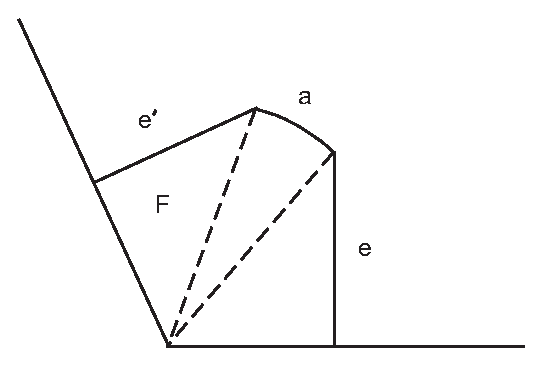
\includegraphics{PS/diag-face.eps}
  \caption{A planar region.}
  \label{fig:face}
\end{figure}

{\bf Case 1. Circumradius of $S$ is less than $\sqrt2$:}  We show
that this case does not occur.  If none of the edges of this
simplex pass through a barrier, then this simplex belongs to
$\CalQ_0'$, a case already considered.  By definition of the
wedges, the edges $\{0,v\}$, $\{0,w\}$, $\{0,w'\}$, $\{v,w\}$, and
$\{v,w'\}$ do not pass through a barrier.  Since five of the six
edges do not pass through a barrier, and since $S$ is formed by
consecutive triangles in the fan around $\{0,v\}$, the sixth does
not pass through a barrier either, by Lemma~\ref{lemma:sixth}.

%This leaves $\{w,w'\}$, which must pass through a barrier
%$T=\{u,u',u''\}$.

%No edge of the barrier $T$ can be $\{0,v\}$ because then $T$ would
%be a triangle in the fan between $w$ and $w'$, which are assumed
%to be consecutive.  No edge of $T$ can pass through a face of $S$
%because its circumradius is less than $\sqrt2$ and
%Lemma~\ref{lemma:no-pass-sqrt2}.  No other edge of $S$ can pass
%through $T$ by Lemma~\ref{lemma:single-enclosed}.  It is now
%apparent that $T$ cannot be placed anywhere at all.  This case
%cannot occur.


{\bf Case 2. Circumradius of $S$ at least $\sqrt2$:} Let
$r\ge\sqrt2$ be the circumradius.   We claim that the edge $e$
cannot extend beyond the wedge through the half plane through
$\{0,v,w'\}$.  In fact, the circumcenter of $\{0,v,w,w'\}$ lies on
the extension (in one direction or the other) of the segment $e$
to a point at distance $r$ from the origin.  If this circumcenter
does not lie in the wedge, then the orientation is negative along
one of the faces $\{0,v,w\}$ or $\{0,v,w'\}$. This face must have
circumradius at least $\sqrt2$, by Lemma~\ref{lemma:sqrt2-chi+},
and this forces the face to be a barrier.  If the orientation is
negative along a barrier, then the simplex $\{0,v,w,w'\}$ is a
simplex in $\CalQ_0$ (Lemmas~\ref{lemma:neg-orient-quad} and
\ref{lemma:neg-orient-tet}). This is contrary to our assumption
above that $\{0,v,w,w'\}$ is not in $\CalQ_0$.




%We observe that the arc marked on a unit sphere coming from a
%barrier is always as least as long as the radius marked on a unit
%sphere coming from a cone $C(u)$.  To see this, we note that the
%arc radius cut out on the unit sphere from the radial projection
%of $u$ to the edge of the cone $C(u)$ is
%$\arc(|u|,\sqrt2,\sqrt2)$. The arc cut out by an edge $\{u,u'\}$
%of a barrier $\{u,u',0\}$ is at least
%$\arc(|u|,\sqrt8,2)\ge\arc(|u|,\sqrt2,\sqrt2)$.  This establishes
%the observation.

These comments show that Figure~\ref{fig:face} correctly
represents the basic shape of $F$, with the understanding that the
edges $e$ and $e'$ may degenerate to a point.  By construction,
every point $x$ in the open convex hull $\{F,0\}$ of $F$ and $0$
lies in $C'(v)\subset \op{VC}(0)$. The convex hull $\{F,0\}$ is
the union of three solids, two Rogers simplices along the
triangles $\{0,v,w\}$ and $\{0,v,w'\}$ respectively, and the conic
solid given by the convex hull of the arc $a$, $v/2$ and $0$. By
Lemmas~\ref{lemma:rogers-app} and \ref{lemma:wedge}, these solids
have density at most $\doct$.

%By Lemma~\ref{lemma:sqrt2-unobstructed}, the origin is not
%obstructed at $x$.  Hence, if $x$ lies in the $V$-cell at $u\ne0$,
%then $|u-x|\le\sqrt2$ and $|x|\le\sqrt2$. This means that $x$ lies
%in the intersection of cones $C(v)\cap C(u)$.

%For there to be a nonempty intersection $\emptyset\ne C(v)\cap
%C(u)$, the circumradius of $\{0,v,u\}$ must be less than $\sqrt2$.
%We consider two cases depending on whether $u$ is some vertex
%$w_j$ (that is, part of the fan).

%Assume the vertex $u=w_j$ is part of the fan.  If $u=w$ or $u=w'$,
%then by construction, no point of $\{F,0\}$ is closer to $u$ than
%to the origin.  (Truncation along the edges $e$ and $e'$
%accomplishes this.) If $u\ne w,w'$, then the parts of $C(v)$ in
%the $V$-cell at $u$ lie in the two wedges alongside the leaf
%$\{0,v,u\}$ of the fan. Thus no such point lies in the wedge in
%question.  Lemma~\ref{lemma:V-cell-local} keeps the $V$-cell from
%leaking past one leaf of the fan to the next.

%Assume that the vertex $u$ is not part of the fan.  By
%construction, we have that the circumradius of $\{0,u,v\}$ is less
%than $\sqrt2$, so that some  edge of $\{0,u,v\}$ crosses a barrier
%$T$ .  The edge that crosses cannot be $\{0,v\}$ because it is too
%short (see Lemma~\ref{lemma:2t0-doesnt-pass-through}).  Let
%$\{u',u''\}\subset \{0,u,v\}$ be the edge passing through $T$.

%{\bf Case-3-b-i. The edge $\{u,v\}$ passes through $T$:} By
%Lemma~\ref{lemma:eta-barrier} at least one-endpoint of $\{v,u\}$
%forms a simplex in $\CalQ_0$ with the barrier, and $0$ is a vertex
%of $T$.  By the observation above, if there is intersection of
%$C(u)$ and $C(v)$, it must be in the convex hull of $T$ and
%$\{u,v\}$.

%If $|v|\le 2t_0$ and $\{T,v\}\not\in\CalQ_0$, then there is not
%overlap in this convex hull by Lemma~\ref{lemma:cone-avoidance}.
%If $\{T,v\}\in\CalQ_0$, then it follows that $\{w,w'\}\subset T$
%and this falls into Case~1, which has already been considered.
%Assume that $|v|\ge 2t_0$. By geometric considerations
%    $$|u-v| \ge \CalE(S(2,2,2,2t_0,2t_0,\sqrt8,2,2,2t_0)  >
%    2.77.$$
%Thus, the circumradius of $\eta(0,u,v)$ is at least
%$\eta(2.51,2.77,2) > \sqrt2$.  This is contrary to the hypothesis
%that $\eta(0,u,v)\le\sqrt2$.  Thus, this case does not occur.

% This means that we have one of
%the situations of Figure~\ref{fig:tricone}. In each case there is
%no overlap between $C(u)$ and $C(v)$, except possibly in points
%over a simplex in $\CalQ_0$.  We have used
%Lemma~\ref{lemma:cone-avoidance}, which separates the cones $C(u)$
%and $C(v)$ from the simplices in $\CalQ_0$. Thus no point of
%$\op{VC}(u)$ meets $\{F,0\}$.

%{\bf Case-3-b-ii. The edge $\{u,0\}$ passes through $T$:}  By
%Lemma~\ref{lemma:eta-barrier}, $v$ is a vertex of $T$, and either
%$\{0,T\}$ or $\{u,T\}$ is a simplex in the $Q$-system.

%Assume $S=\{0,T\}$ is in the $Q$-system.  If $x$ is not in the
%cone over $S$, then Lemma~\ref{lemma:V-cell-local} bounds the
%$V$-cell at $u$ away from $x$.  If $x$ lies in the cone over $S$,
%then $T=\{v,w,w'\}$, where $\{0,v,w\}$ and $\{0,v,w'\}$ are
%consecutive triangles in the flag around $\{0,v\}$.  This
%situation was treated in Case 1.

%Assume that $S=\{u,T\}$ is a simplex in the $Q$-system, and that
%$\{0,T\}$ is not a simplex in the $Q$-system.   Let $H$ be the
%convex hull of $T$, $u$ and $0$. If $x$ lies outside this convex
%hull, then $x$ cannot lie in the interior of both $B(u,\sqrt2)$
%and $B(0,\sqrt2)$. In fact, the shortest path outside $H$ from $0$
%to $u$ has length at least $\sqrt2$ along a face of $\{0,T\}$ and
%length an additional $\sqrt2$ along a face of $\{u,T\}$.

%Lemma~\ref{lemma:sqrt2-unobstructed} implies that $x$ cannot
%belong to $S$.  Assume that $x$ belongs to $H$. Then $x$ lies in
%the convex hull of $\{0,T\}$.  The vertex $u$ is then obstructed
%at $x$ through the barrier $T$.  Thus $x$ does not lie in the
%$V$-cell at $u$.

%This completes the proof of the claim: all points $x$ in the open
%convex hull $\{F,0\}$ of $F$ and $0$ lie in the $V$-cell at $0$.
%To complete the proof, we show that this convex hull has density
%at most $\doct$.



This completes the proof that $\sigma_R(D)$ is never positive on
non-triangular standard regions $R$.  Note that the decomposition
into the parts of cones $C'(v)$ inside a wedge is compatible with
the partition of the unit sphere into standard regions, so that
the estimate holds over each standard region, and not just over
the union of the standard regions.
%
\end{proof}






\begin{lemma}  If $R$ is a standard region that is not a triangle,
and if $\sigma_R(D)=0$, then $(R,D)$ is a quad cluster.  Moreover,
the four corners of $R$ in the quad cluster have height $2$,
forming a square of side $2$.
\end{lemma}

\begin{proof}
To analyze the case of equality, first we note that any truncation
at $1.18$ produces a strict inequality (Lemma~\ref{lemma:cone} is
strict if the volume is nonzero), so that every point must lie
over a simplex in $\CalQ_0'$ or over some $C'(v)$. We have
$\svor(S)<0$ for simplices with circumradius less than $\sqrt2$.
The only simplices in $\CalQ_0$ that produce equality are those
with five edges of length $2$ and a diagonal of length $\sqrt8$.
Any nontrivial arc $a$ produces strict inequality (see
Lemma~\ref{lemma:wedge}, so we must have that $e$ and $e'$ meet at
exactly distance $\sqrt2$ from $0$ and $v$.  Moreover, if $e$ does
not degenerate to a point, the corresponding Rogers simplex gives
strict inequality, unless $\{0,v,w\}$ is an equilateral triangle
with side length $2$.  We conclude that the entire part of the
$V$-cell over the standard region must be assembled from Rogers
simplices $R(1,\eta(2,2,2),\sqrt2)$, and quarters with lengths
$(2,2,2,2,2,\sqrt8)$.  This forces each vertex $v$ of height at
most $2t_0$ to have height $2$.  It forces each pair of triangles
$\{0,v_1,v_2\}$ $\{0,v_2,v_3\}$, that determine consecutive edges
along the boundary of the standard region to meet at right angles:
    $$\dih(0,v_2,v_1,v_3)=0.$$
This forces the object to be a quad cluster of the indicated form.
\end{proof}

We conclude the \chap\ with a proof of the main theorem.  With all
our preparations in place, the proof is short.

\begin{proof} {\bf Theorem~\ref{lemma:local-optimality} (Local
Optimality)} The hypothesis implies that there are $6$ quad clusters
and $8$ quasi-regular tetrahedra at the origin of the decomposition
star. By Lemma~\ref{lemma:1pt}, each quasi-regular tetrahedron
scores at most $1\,\pt$ with equality if and only if the tetrahedron
is regular with edge-length $2$.  By Theorem~\ref{lemma:quad0}, each
quad cluster scores at most $0$, with equality if and only if the
corners of the quad cluster form a square with edge-length $2$ at
distance $2$ from the origin. Thus, $\sigma(D)$ is at most $8\,\pt$.
In the case of equality, there are $12$ vertices at distance $2$
from the origin, forming $8$ equilateral triangles and $6$ squares
(all of edge-length $2$). These conditions are satisfied precisely
when the arrangement is $U_{fcc}$ or $U_{hcp}$ up to a Euclidean
motion.
\end{proof}

    \chapter{Geometric Detail}%DCG "The S-System" Sec.9, p85
    \label{sec:fine}
    \oldlabel{2}

The previous chapter gives the constructions
needed in the top-level description of the proof.  
These constructions do not take us far.   This
chapter gives the details of geometric constructions that
will be used to carry the proof to completion. 
We have discussed many of these constructions before, such
as V-cells, the Q-system, fans, and fitted crowns.  In this
chapter we look at how these structures are interrelated.

\section{Interaction}


%Let $\CalQ=\CalQ(\Lambda)$ be the $Q$-system.  
%For $v\in\Lambda$, let $\CalQ(\Lambda,v)$ be the subset
%of those with a vertex at $v$.\index{Qv@$\CalQ(\Lambda,v)$}
%% Defined already. def:q-system.


\begin{lemma} \tlabel{lemma:voronoi-truncation-over-Q}\rating{100}
Let $(\Lambda,v_0)$ be a centered packing.  Let $X$ be the union
of the sets $\op{aff}_+(v_0,\{v_1,v_2\})$ as $\{v_0,v_1,v_2\}$
runs over the barriers with a vertex at $v_0$.  Let $Z$ be the
union of the following tips:
   $$
   \op{aff}_+^0(v_0,\{v_1,v_2,v_3\}) \cap \op{aff}_-
   (\{v_1,v_2,v_3\},v_0)\cap \Omega_2(\Lambda,v_0).
   $$
as $\{v_0,v_1,v_2,v_3\}$ ranges over $\CalQ(\Lambda,v_0)$.
Then 
$$\Omega_2(\Lambda,v_0)
 \subset X\cup Z\cup \op{VC}(\Lambda,v_0).$$
%If $x$ lies in the \index{Voronoi cell} Voronoi cell at $v_0$, 
%but not in the $V$-cell at $v_0$, then there exists a
%simplex $Q\in\CalQ(\Lambda,v_0)$, such that $x$ lies in the cone (at $v_0$)
%over $Q$. Moreover, $x$ does not lie in  $\op{conv}^0(Q)$.
(That is, up to the null set $X$, the $V$-cell contains
the truncated tip-reduced Voronoi cell.)
\end{lemma}

\begin{proof}  Let 
 $$x \in \Omega_2(\Lambda,v_0)
 \setminus (X\cup\op{VC}(\Lambda,v_0)).
 $$
By
the definition of $V$-cell, there is a barrier $\{v_1,v_2,v_3\}$
such that
  $$\op{conv}\{v_1,v_2,v_3\}\cap \op{conv}^0\{v_0,x\}\ne\emptyset.$$ 
We have $v_0\not\in\{v_1,v_2,v_3\}$, for otherwise $x\in X$, 
which is contrary to assumption. 
By tarski\tarf{tarski:vor-bar-tet}\tarf{tarski:vor-bar-quad},
the simplex $Q=\{v_0,v_1,v_2,v_3\}$ is a quasi-regular tetrahedron
or a flat quarter.  If the barrier is the face of a flat quarter,
then $Q$ too is in
the $Q$-system.  By tarski\tarf{tarski:pass-cone},  $x\in\op{aff}_+(v_0,\{v_1,v_2,v_3\})$.  
We get $x\in\op{aff}_+^0(v_0,\{v_1,v_2,v_3\})$ from $x\not\in X$.

We have $x\in\op{aff}_-
   (\{v_1,v_2,v_3\},v_0)$. Otherwise, $\op{conv}^0\{v_0,x\}$ does
not meet $\op{conv}\{v_1,v_2,v_3\}$.
%We have $x\in\op{conv}(Q)\setminus X$. Otherwise, 
%the barrier contains $x$, and the plane through the barrier contains
%$v_0$, so that $\{v_0,v_1,v_2,v_3\}$ is planar.  This is contrary
%to tarski\tarf{tarski:flat-Q}. 
The rest is clear.
\end{proof}



\begin{lemma}\tlabel{lemma:VC-Omega}\rating{100}
Let $(\Lambda,v_0)$ be a centered packing.
Inside the ball of radius $t_0$ at $v_0$, the $V$-cell and
Voronoi cell coincide up to a null set:
   $$B(v_0,t_0)\cap \op{VC}(\Lambda,v_0) \equiv B(v_0,t_0)\cap \Omega(\Lambda,v_0).$$
\end{lemma}

\begin{proof} Let $X$ be the (finite) union of planes equidistant from $v_0$ and $w\in \Lambda(v_0,2t_0)$.  $X$ is a null set.  Let $Y$ be the (finite) union of $\op{aff}_+(w,\{w_1,w_2\})$, for $w\in \Lambda(v_0,2t_0)$ and $\{w,w_1,w_2\}$ a barrier.  $Y$ is a null set.
The Voronoi cells $\Omega(\Lambda,w)$, $w\in\Lambda(v_0,2t_0)$ cover
$B(v_0,t_0)$ except for the null set $X$.  
Suppose that some point  $x\not\in X\cup Y$
lies in $$(B(v_0,\Lambda)\cap\op{VC}(\Lambda,v_0) )\setminus \Omega(\Lambda,v_0).$$
Then $x\in \Omega(\Lambda,w)$, where
$w\ne v_0$.  
% By Lemma~\ref{tarski:unobstr-t0}, 
From $x\not\in Y$, it follows that the point $v_0$ is
unobstructed  at $x$ by tarski\tarf{tarski:unobstr-t0}.  
Thus, $|x-w|< |x-v_0|\le t_0$.  By
tarski\tarf{tarski:unobstr-t0} again, $w$ is unobstructed at $x$, so
that $x\in \op{VC}(\Lambda,w)$, contrary to the assumption
$x\in\op{VC}(\Lambda,v_0)$.  Thus $B(v,t_0)\cap\op{VC}(\Lambda,v_0)\subset\Omega(\Lambda,v_0)$.

Similarly, if $x\in B(v_0,t_0)\cap \Omega(\Lambda,v_0)$ and $x\not\in Y$,
then $x$ is
unobstructed at $v_0$, and $x\in \op{VC}(\Lambda,v_0)$.
\end{proof}

\bigskip

%\begin{remark} The next lemma helps to determine which $V$-cell
%a given point $x$ belongs to.  If $x$ lies in the open cone over a
%simplex $Q_0$ in $\CalQ$, then Lemma~\ref{lemma:Q-divide}
%describes the $V$-cell decomposition inside $Q$;  beyond $Q$ the
%point $v_0$ is obstructed by a face of $Q$, so that such $x$ do not lie
%in the $V$-cell at $v_0$. 
%%If $x$ does not lie in the open cone over
%%a simplex in $\CalQ$, but lies in the open cone over a standard
%region $R$, then Lemma~\ref{lemma:V-cell-local} describes the
%$V$-cell.  
%It states in particular, that for unobstructed $x$, it
%can be determined whether $x$ belongs to the $V$-cell at the
%point $v_0$ by considering only the vertices $w$ that lie in the closed
%cone over $R$ (the standard region containing the radial
%projection of $x$). In this sense, the intersection of a $V$-cell
%with the open cone over $R$ is {\it local\/} to the cone over $R$.
%\end{remark}
%


Let $\CalB_0'$ be the set of triangles $T$ such that at least one
of the following holds:
\begin{itemize}
    \item $T$ is a barrier at $v_0$, or
    \item $T=\{v_0,v,w\}$ consists of a diagonal of a quarter in the
    $Q$-system together with one of its anchors.
\end{itemize}

%DCG Lemma 5.29, page 50.
\begin{lemma} [Decoupling Lemma]\tlabel{lemma:V-cell-local}\rating{100}
%Let $x\in I_0$, the cube of side $4$ centered at $v_0$
%parallel to coordinate axes. 
Let $(\Lambda,v_0)$ be a centered packing.  Let $\{v_0,v_1,v_2,w\}$
be a set of four vertices of $\Lambda$. 
Assume that the closed segment
$\op{conv}\{x,w\}$ intersects $\op{aff}_+(v_0,\{v_1,v_2\})$, where
$F = \{v_0,v_1,v_2\}\in \CalB'_0$. Assume that $v_0$ 
is not obstructed at $x$. Assume that $x$ is closer to $v_0$ 
than to both $v_1$ and $v_2$. Then $x\not\in\op{VC}(\Lambda,w)$.
\end{lemma}
\index{decoupling lemma}

%\begin{remark}  The Decoupling Lemma is a crucial result.  It
%permits estimates of the scoring function in
%Chapter~\ref{sec:scoring} to be made separately for each standard
%region.  The estimates for separate standard regions are far
%easier to come by than estimates for the score of the full
%centered packing.  
%\end{remark}

\begin{proof}
Assume for a contradiction that $x$ lies in $\op{VC}(\Lambda,w)$. In
particular, we assume that $w$ is not obstructed at $x$.  Since
$v_0$ is not obstructed at $x$, $w$ must be closer to $x$
than $x$ is to $v_0$.

By tarski\tarf{tarski:decouple}, 
   $|w-v_0|,|w-v_1|,|w-v_2|\le 2t_0$.  Thus, $Q=\{v_0,w,v_1,v_2\}$ is
a quarter or a quasi-regular tetrahedron.  By the definition of
$\CalB'_0$, the face $F$ must lie in the $Q$-system.  Thus,
$F$ is a barrier.  Again, by tarski\tarf{tarski:decouple},
$\op{conv}(F)$ meets the segment from $x$ to $w$, so $x$ is obstructed
at $w$.  Thus, $x$ does not lie in $\op{VC}(\Lambda,w)$.
\end{proof}

%\section{Local Optimality}%DCG Sec. 8, p72  
%\tlabel{sec:local-opt}
%Moved after the main estimate.




\section{Fitted Crown}%DCG 9.1, p95
    \label{sec:fine-overview}
    \oldlabel{2.1}




\subsection{crown tuple}%DCG 9.2, p86
    \label{sec:deltaP}
    \oldlabel{2.3}

Section~\ref{sec:anc} defines a region called fitted crowns.  We study
fitted crowns further in the context of $V$-cells and the $Q$-system
of a sphere packing.  Fitted crowns $FCR$ are defined at the same time
as various auxiliary sets $FC$, $\FCinner$, $\rogFC$ in
Definition~\ref{def:fitted-crown}.  The reader is advised to review those
definitions before continuing.

\begin{definition}\label{def:eta0}
Set $\eta_{V0}(v,w) = \eta(|v-w|,2,2t_0)$. 
\index{zzeta@$\eta_{V0}$}
\end{definition}

%By tarski\tarf{tarski:1453}, 
%if $h\le\sqrt2$, then $\eta(2h,2,2t_0)\le \eta(2,2t_0,\sqrt2) <
%1.453$.\index{ZZZZ1.453@1.453}



\begin{definition}\label{def:crown-tuple}
Let $\Lambda$ be a packing.
We say that a four-tuple $(v_0,v,u,w)$ of vertices in $\Lambda$   
is a crown tuple if
\begin{itemize}
  \item $2t_0 < |v-v_0| <\sqrt8$.
  \item $u$ and $w$ are anchors of $\{v_0,v\}$.
  \item $w$ is the successor of $u$ in the azimuth cycle with respect to
   $(v_0,v)$ on the
   anchors of $\{v_0,v\}$.
\begin{enumerate}  
    \item Either $\op{azim}(v_0,v,u,w)\ge\pi$, or
    \item $\op{azim}(v_0,v,u,w) <\pi$, 
 $|u-w|\ge 2.77$,
    $\rad_V(v_0,v,u,w)\ge\eta_{V0}(v,v_0)$, and the max of 
    $\eta_V(v_0,u,w)$ and $\eta_V(v,u,w)$ is
    $\ge\sqrt2$.
    \label{enum:wedge2}
\end{enumerate}
\end{itemize}
\index{crown tuple}
We say that $(v_0,v,u,w,\epsilon)$, with $\epsilon\in\{\pm1\}$ is
a signed crown tuple if $\epsilon=1$ and $(v_0,v,u,w)$ is a crown tuple
or if $\epsilon=-1$ and $(v_0,v,w,u)$ is a crown tuple.
\index{signed crown tuple}
\end{definition}

The definition of fitted crown relies upon Assumption~\ref{eqn:q1q2}.
The assumption is always satisfied for a crown tuple.

\begin{lemma}\tlabel{lemma:fitted-q1q2}\rating{100}
Let $\Lambda$ be a sphere packing with crown tuple
$(v_0,v,w_1,w_2)$.  Let $c_1=c_2=\eta_{V0}(v_0,v)$. 
Then Assumption~\ref{eqn:q1q2} holds for $(v_0,v,w_1,w_2,c_1,c_2)$.
\end{lemma}

\begin{proof} XX REDO PROOF. Assume not.  
We use the notation of Section~\ref{sec:anc}.
We can decrease $\op{azim}(v_0,v,w_1,w_2)$
until $\op{azim}<\pi$.  Let $S=\{v_0,v,w_1,w_2\}$.
$2.77 \le |w_1-w_2|$ implies that the simplex $S$
has positive orientation at $w_1$ and $w_2$ (Lemma~\ref{XX}). 
The circumcenter $p$ can be written, 
   $$p + p_1 + s_1 u_1 = p_2 + s_2 u_2,\quad s_1,s_2 > 0.$$
If Assumption~\ref{eqn:q1q2} fails,
   $$\op{azim}(v_0,v,w_1,q_2) < \op{azim}(v_0,v,w_1,q_1).$$
Then the circumradius $|p-v_0|$ is
   $$\rad_V(v_0,v,w_1,w_2) < \eta_{V0}(v_0,v).$$
This contradicts the definition of crown tuple.
\end{proof}



%Fix $i,j$, with $j\equiv i+1\mod k$. If $W = W_i$ is a crown tuple, 
%let $\{v_0,v_i,v\}^\perp$ be the plane through $v_0$ and
%the circumcenter of $\{v_0,v_i,v\}$, perpendicular to $\{v_0,v_i,v\}$.
%Skip the following step if the circumradius of $\{v_0,v_i,v\}$ is
%greater than $\eta_{V0}(v,v_0)$, but if the circumradius is at most
%this bound, the plane
%of $\{v_0,v_i,v\}^\perp$
%intersects the right circular cone boundary of $D_0$ along two rays
%emanating from $v_0$.  Let $c_i$ be a point on the ray (selected on
%the $W$-side of $\{v_0,v_i,v\}$).  Simlarly, we construct the point
%$c_i'$ for $\{v_0,v,v_j\}$ (again on the $W$-side).
%
%Define $\theta=\theta(v)$ by $\cos\theta = |v-v_0|/(2\eta_{V0}(v,v_0))$.
%If Condition~2 holds, we let $c$ be the 
%circumcenter of $\{v_0,v_i,v_j,v\}$.  The angle
%at $v_0$ between $c$ and $v$ is
%$\theta'$, where
%$$\cos\theta' = |v-v_0|/(2\rad)\le |v-v_0|/(2\eta_{V0}) = \cos\theta.$$
%We conclude that $\theta'\ge\theta$ and $c$ does not lie in $D_0$.
%Thus, the half-planes
%   $$
%   A_i,\quad B_i=\op{aff}_+(\{v_0,v\},c_i),\quad 
%   B'_i = \op{aff}_+(\{v_0,v\},c'_i), \quad
%   A_j
%   $$
%are ordered cyclically around $\{v_0,v\}$. (Set $B_i=A_i$
%or $B'_i=A_j$, if the corresponding circumradius is greater than
%$\eta_{V0}(v,v_0)$.)
%Let $W'=W'_i$ be the open wedge of $D_0$ between $B_i$ and $B'_i$.
%Let
%    $$E_w = \{x : 2 x\cdot w \le w\cdot w\},$$
%for $w = v,v_i,v_j$. These are half-spaces bounding the Voronoi
%cell. Set $E_\ell = E_{v_\ell}$.
%

%
%\begin{definition} \label{def:delta-e}
%In both cases (Conditions~1 and~2), let $W$ be the wedge between
%$v_i$ and $v_j$ along $(v_0,v)$, $W'$ the smaller wedge, 
%and let $c=\eta_{V0}(v,v_0)$ in
%    $$
%    \begin{array}{lll}
%      \FC'(v,W) &= [E_v\cap W'\cap D_0]\cup \op{rog}^0(v_0,v,v_i,p_i,c)
%      \cup \op{rog}^0(v_0,v,v_j,p_j,c)
%      \\
%    \FC(v,W) &= \FC'(v,W) \cup 
%    \op{rog}^0(v_0,v_i,v,p_i,c)
%    \cup \op{rog}^0(v_0,v_j,v,p_j,c)\\
%    \bigd(v,W) &= \{x\in\FC(v,W)\mid |x-v_0|>t_0\},
%    \end{array}
%    $$
%where $p_i,p_j$ are selected so that the simplices $\op{rog}^0$ lie
%in the wedge $W$.
%\index{zzdelta@$\bigd(v,W)$}
%\index{zzDelta@$\FC(v,W)$}
%\end{definition}
%

%\begin{remark} We note that the union is actually a disjoint union,
%and that each of the pieces is one of the primitive regions, so
%the volume of $\FC$ is immediate.
%\end{remark}





\begin{remark}
Recall that a Rogers simplex (Definition~\ref{def:rog}) is defined to be the
empty set 
if the corresponding parameters are not coherent.  It is to
be understood that the all discussion regarding this set
can (and should) be disregarded in the case that it is empty.
\end{remark}



\subsection{normal tuple}


The following definition will be used briefly, then discarded.
Its purpose is to group together a few cases in the next
few lemmas.

\begin{definition}  Let $(v_0,v,u_1,u_2)$ be a tuple of vertices
in a packing $\Lambda\subset\ring{R}^3$.  We say that it is {\it normal} if $2t_0<|v-v_0|<\sqrt8$
and one of the
following holds:
\begin{enumerate}
  \item (qrt) $\{v_0,u_1,u_2\}$ is a quasi-regular triangle.
  \item (upright) $\{v_0,u_1,u_2\}$ is an upright triangle; that is, say,
    $2t_0 < |u_1-v_0| < \sqrt8$, and $u_2$ is an anchor of $\{v_0,u_1\}$.
    (or vice-versa, swapping $u_1$ with $u_2$).
  \item (flat)
   $2t_0<|u_1-u_2|<\sqrt8$; and if $u_1,u_2$ are both anchors of
   $\{v_0,v\}$, 
   then
    no further anchor of $\{v_0,v\}$
   lies in the lune $\op{aff}^0_+(\{v_0,v\},\{u_1,u_2\})$.
\end{enumerate}
\end{definition}



In the following lemmas, we adopt a uniform notation.  Let $(\Lambda,v_0)$ be a centered packing, upright diagonal 
$\{v_0,v\}$, signed crown tuple
$(v_0,v,w,w',\epsilon)$.
%Set $R_w=\rogFC(v_0,v,w,w',\epsilon)$.
%R_w=\op{rog}^0(v_0,w,v,p,\eta_{V0}(v,v_0))$,
%where $p$ is selected so that $R_w$ lies in $W(v_0,v,w,w')$.

\begin{lemma}\tlabel{lemma:meet-normal}\rating{80}
Let $(\Lambda,v_0)$ be a centered packing.  Let $\{v_0,u_1,u_2\}$
be a barrier.  Let $(v_0,v,w_1,w_2)$ be a crown tuple.  If
$\FC(v_0,v,w_1,w_2)$ meets $F=\op{aff}_+(v_0,\{u_1,u_2\})$, then
$(v_0,v,u_1,u_2)$ is normal.
\end{lemma}

\begin{proof} We have $\FC\subset \op{aff}_+^0(\{v_0,v\},\{u_1,u_2\})$
and $F\subset \op{aff}_+(\{v_0,v\},\{u_1,u_2\})$.
Continue. XX
\end{proof}

\begin{lemma}\tlabel{lemma:new-anchor}\rating{50}
Let $(\Lambda,v_0)$ be a centered packing
  Let $S=\{v_0,v,w,u\}$ be a simplex in $\Lambda$.  Assume that $\{v_0,v\}$ is an
upright diagonal, that $w$ and $u$
are anchors of $\{v_0,v\}$, and that $\rad_V(S)< \eta_{V0}(v,v_0)$.
Assume there is a crown tuple $(v_0,v,w,w')$
extending the triple $(v_0,v,w)$
(on the same side of the face as $u$).  
Then the anchor $w'$ of $\{v_0,v\}$ lies between $u$ and $w$
(that is,  $w'\in\op{aff}_+^0(\{v_0,v\},\{u,w\})$) with
    $|w'-w|\ge2.77$ and
    $\rad\{v_0,w,w',v\} \ge \eta_{V0}(v,v_0)$.
\end{lemma}

\begin{proof} The conditions on $(v_0,v,w,u)$ are incompatible with the
conditions of Definition~\ref{def:crown-tuple} defining crown tuples.
Therefore, $w$ and $u$ cannot be consecutive anchors around
$\{v_0,v\}$.  Let $w'$ be the anchor such that $(v_0,v,w,w')$
is a crown tuple.  Since $w$ and $w'$ are consecutive anchors,
we see that $w'$ must be between $u$ and $w$.  It must have the
second type in Definition~\ref{def:crown-tuple}.  The conclusion follows.
\end{proof}



\begin{lemma}\tlabel{lemma:FC-}\rating{80}  
Let $S=(v_0,v,u_1,u_2)$ be normal and
let $S'=(v_0,v,w_1,w_2)$ be a crown tuple in a packing $\Lambda$.
Let $a = |v-v_0|/(2\eta_{V0}(v_0,v))$.  
Then
$$
 \op{rcone}^0(v_0,v,|v-v_0|/(2\eta_{V0}(v_0,v))) \cap
  \op{aff}^0_+(\{v_0,v\},\{w_1,w_2\})
$$
does not meet $F=\op{cone}(v_0,\{u_1,u_2\})$.
In particular, the subset
$\FCinner(S')$ does not meet $F$.
\end{lemma}

\begin{proof}  Assume for a contradiction that the sets meet.
Tarski\tarf{tarski:eps-bigd-}
implies that $S$ is normal of the flat or qrt variety, and 
that $u_1$ and $u_2$ are anchors of $\{v_0,v\}$.  
The result also gives that 
$\rad_V(S)<\eta_{V0}(v,v_0)$.    
In the qrt case, $S$ forms
an upright quarter.  By tarski\tarf{tarski:consec-anchors}, $u_1$ and $u_2$
are consecutive anchors. In the flat case as well, 
$u_1$ and $u_2$ are consective
anchors around $\{v_0,v\}$.

The set $\{u_1,u_2\}$ is not $\{w_1,w_2\}$ because $(v_0,v,u_1,u_2)$
does not satisfy the properties of a crown tuple (assuming $u_1,u_2$
indexed so that $\op{azim}(v_0,v,u_1,u_2) = \dih_V(\{v_0,v\},\{u_1,u_2\})$).  The anchors $u_1,u_2$ are consecutive, as are $w_1,w_2$.
The set $\FCinner(S')$ lies in the lune $\op{aff}_+^0(\{v_0,v\},\{w_1,w_2\})$ and $F$ lies in the lune $\op{aff}_+(\{v_0,v\},\{u_1,u_2\})$.
These lunes are disjoint.
%
%If the crown tuple $S'$ is not in $W(v_0,v,u_1,u_2)$, 
%then $\FC$ lies outside the 
%lune $\op{aff}_+^0(\{v_0,v_0\},\{u_1,u_2\})$, but $F$ lies in it.  Thus,
%the crown tuple must run between $u_1$ and $u_2$.   This contradicts 
%the rules for forming crown tuples.  (Lemma~\ref{lemma:new-anchor} 
%implies that
%anchors $u_1$ and $u_2$ cannot be consecutive.)
\end{proof}

\begin{lemma}\tlabel{lemma:fine-Rw}\rating{50}
Let $S=(v_0,v,w,u_1)$ be normal and $(v_0,v,w,w',\epsilon)$ a signed crown tuple
of a packing $\Lambda$.  
Then
$\rogFC(v_0,v,w,w',\epsilon)$
does not meet $F=\op{cone}(v_0,\{w,u_1\})$.
\end{lemma}

\begin{proof}  We can use the same proof as in Lemma~\ref{lemma:FC-},
except with one tarski\tarf{tarski:eps:fine:Rw} calculation 
substituted for 
another\tarf{tarski:eps-bigd-}.
\end{proof}

%% This has been replaced with tarski:fine:Rw:u.
%% In fact the proofs are almost the same.
%% It can be deleted.

%\begin{lemma}\tlabel{lemma:fine:barrier}  
%Let $S=\{v_0,v,w,u\}$ be a set of four distinct vertices
%in a packing $\Lambda$.  
%Assume that $\{v_0,v\}$ is an upright diagonal of
%a quarter in the $Q$-system and that $w$ is an anchor of $\{v_0,v\}$.
%Let $R_w$ be as above; that is, a Rogers simplex attached to a crown tuple 
%extending $(v_0,v)$.
%Assume $x\in R_w$ satisfies $\epsilon_0(x,\{v,w,u\})= u$.
%Then there exists a vertex $w'$ that is an anchor of $\{v_0,v\}$ such
%$b=\{v,w',v_0\}$ is a barrier and $x$ is obstructed from $u$
%by $b$.
%\end{lemma}
%
%\begin{proof} Assume for a contradiction that $\epsilon_0(x)=u$.
%We separate the proof into two cases, depending on whether
%$x$ and $u$ lie on the same side of $A=\op{aff}(v,w,v_0)$.
%
%Assume that $x$ and $u$ lie on opposite sides of $A$.
%For any nonzero vertices $v',v''$,
%Let $L(v',v'')$ be the line of points equidistant from $\{v_0,v',v''\}$.
%The three lines $L(u,v)$, $L(v,w)$, $L(u,w)$ meet at the circumcenter
%$c$ of $S$.  The rays $L^+(u,v)$, $L^+(v,w)$, $L^+(u,w)$ demarcate
%the regions between $\epsilon_0=w,u,v$.  (Pick the direction
%of ray so that it runs through the circumcenter of the face $\{v_0,v',v''\}$
%if the remaining vertex has positive orientation, and so that it
%runs in the opposite direction otherwise.)
%
%If $u$ has positive orientation in $S$, then $L^+(v,w)$ runs through
%the circumcenter of $\{v_0,v,w\}$ and along an edge of $R_w$.
%The point $w/2$ in the closure of  $R_w$ also has $\epsilon_0=w$.
%It follows that $\epsilon_0$ has value $w$ on $R_w$, which is contrary
%to our assumption.
%
%Thus, $u$ has negative orientation in $S$.  
%This implies that $|u-v|,|u-w|,|u-v_0|\le 2.51$.  In particular,
%$S$ is a quarter.  Since it has the same diagonal as a quarter in
%the $Q$-system, we have that $S$ is in the $Q$-system, so that
%$\{v_0,v,w\}$ is a barrier.  By tarski\tarf{tarski:tip-cone}, we have
%that $x\in \op{cone}(u,\{v,w,v_0\})$.  In particular, $x$ is obstructed
%from $u$ by the barrier $\{v,w,v_0\}$.  Take $w'=w$ in this case.
%
%Now assume that $x$ and $u$ lie on the same side of $A$.
%First consider the special case where
%we also have that $\rad_V(S)\ge \eta_{V0}(v,v_0)$ and that that
%the orientation of $u$ is non-positive in $S$.  In this case, it
%follows that $S$ is a quarter in the $Q$-system.  By the rule
%for constructing crown tuples, there is no $R_w$ along $\{v_0,v,w\}$
%in this case.  Next consider the case where
%$\rad_V(S)\ge \eta_{V0}(v,v_0)$ and the orientation of $u$ is positive
%in $S$.  In this case, the ray $L^+(v,w)$ runs along the edge of 
%$R_w$ as before, and we see that $\epsilon_0=w$ on $R_w$.
%
%Finally consider the case where $\rad_V(S)<\eta_{V0}(v,v_0)$.
%It follows that $u$ is an anchor of $\{v_0,v\}$.
%By Lemma~\ref{lemma:new-anchor}, there exists a further anchor
%$w'$ between $u$ and $w$.  By tarski\tarf{tarski:prev},
%$\op{conv}\{x,u\}$ meets $\op{conv}\{v_0,v,w'\}$, and
% $|u-w'|\le 2.51$.  In particular $S'=\{v_0,v,w',u\}$ is
%an upright quarter and $\{v_0,v,w'\}$ is a barrier.
%\end{proof}



\begin{lemma}\tlabel{lemma:fine-Rw:5}\rating{300}
Let $\{v_0,v,w,u_1,u_2\}$ be a set of five distinct vertices in a
centered packing $(\Lambda,v_0)$.
packing.  Assume that $\{v_0,v\}$ is an upright diagonal of a quarter
in the $Q$-system and that $w$ is an anchor of $\{v_0,v\}$.
Assume that $S=(v_0,v,u_1,u_2)$ be normal.
Let $\rogFC(v_0,v,w,\ldots)$ be as above; that is, a Rogers simplex attached to a signed crown tuple $(v_0,v,\ldots)$.
Then $\rogFC$ does not meet $F=\op{cone}(v_0,\{u_1,u_2\})$.
\end{lemma}



\begin{proof}
For a contradiction, assume these sets meet at $x\in \rogFC(v_0,v,w,\ldots)\cap F$.
%We have $\epsilon_0=\epsilon_0(x,\{w,u_1,u_2\})\in\{w,u_1,u_2\}$.  We consider
%two cases depending on whether $\epsilon_0=w$.
Tarski\tarf{tarski:fine-Rw-split} enumerates six different possible
configurations of points $\{v_0,v,w,u_1,u_2\}$.  We discuss each
in turn.

In the first three cases, 
%
%Assume that $\epsilon_0=w$.  By tarski\tarf{tarski:fine:Rw:5},
we have $|w-u_1|\le 2.51$ and $|w-u_2|\le 2.51$.  The first is that
for either $u=u_1$ or $u=u_2$, we have that $(v_0,v,w,u)$ is normal
and that $\rogFC(v_0,v,w,\ldots)$ meets $\op{cone}(v_0,\{w,u\})$.  This is contrary to
Lemma~\ref{lemma:fine-Rw:5}.

The second possibility is that
$2.51<|u_1-u_2|<\sqrt8$ and that $v\in\op{cone}^0(v_0,\{u_1,u_2,w\})$
with $u_1,u_2,w$ all anchors of $\{v_0,v\}$.  By the normality
hypothesis, these are the only anchors of $\{v_0,v\}$.  None of the
corresponding tuples are crown tuples extending
$(v_0,v)$.  Thus, this case does not
occur. 

The third possibility is that $w\in \op{aff}_+(\{v_0,v\},\{u_1,u_2\})$
and $2.51<|u_1-u_2|$.  This is contrary to the normality
condition on $S$.

%In the remaining case, we have $\epsilon_0=u\in\{u_1,u_2\}$.  
%Let $S'=\{v_0,v,w,u\}$.  
In the remaining cases, there is a 
relabeling of vertices $\{u,u'\}=\{u_1,u_2\}$.
In the fourth case, we have that $\{v_0,v,u,w\}$ is an upright
quarter and $u'\in \op{aff}_+^0(\{v_0,u\},\{v,w\})$.  Inspecting
the various possibilities for $u'$, we find that
$\op{conv}\{u,u'\}$ meets $\{v_0,v,w\}$.  This forces $u'$ to be
an anchor of $\{v_0,v\}$ and $2.51 < |u-u'|$.  By normality
$u,u'$ are consecutive anchors.  But this if false, because the
anchor  $w$ is between them.
%By Lemma~\ref{lemma:fine:barrier}, there
%exist a barrier $b=\{v_0,v,w'\}$ such that $x$ is obstructed from
%$u$ by $b$.  However, if $x\in\op{cone}(v_0,\{u_1,u_2\})$, then
%there exists no such obstruction.  Thus, the intersection
%is empty.

In the fifth case, $\{v_0,v,u,w\}$ is an upright quarter and
$\rogFC(v_0,v,w,\ldots)\subset \op{aff}_+(\{v_0,v,w\},u)$.  By Lemma~\ref{lemma:new-anchor},
there is an anchor $w'$ of $\{v_0,v\}$ between $u$ and $w$.
This is not possible for geometric reasons. XX detail.

In the sixth case, $u_1$ and $u_2$ are anchors of $\{v_0,v\}$.
They are not consecutive and $2.51 < |u_1-u_2|$.  This contradicts
the definition of normal.
We have examined all six cases.  In each case, the assumption
that $F$ and $R$ meet leads to a contradiction.  The result follows.
\end{proof}

\subsection{fitted crown and fan}

\begin{lemma}\tlabel{lemma:delta-tri}\rating{200}
%\tlabel{lemma:delta-upright}
%\tlabel{lemma:delta-flat}
Let $(\Lambda,v_0)$ be a centered packing.
Let $\{v_0,v\}$ be
an upright diagonal of a quarter in the $Q$-system.
Assume that $(v_0,v,u_1,u_2)$ is normal.
Let $E$ be the set of all $\{u,v\}$ such that $\{v_0,u,v\}$
is a barrier.  Set
   $$
   V = \{v \mid \exists u.\quad \{u,v\}\in E\}.
   $$
Assume $(v_0,V,E)$ a fan.  Then, for each crown tuple
$(v_0,v,w_1,w_2)$, there is a component $U\in Y(v_0,V,E)$ such
that $\FC(v_0,v,w_1,w_2)\subset U$.  In particular, $FC$ does
not meet any blades of the fan.
%Let $F=\{v_0,u_1,u_2\}$ be a quasi-regular triangle.   
%Assume that there
%exists a quarter in the $Q$-system along $\{v_0,v\}$.  
%Let $(v_0,v,w_1,w_2)$ be a crown tuple.
%Then
%$\FC(v_0,v,w_1,w_2)$ does not meet $A=\op{aff}_+(v_0,\{u_1,u_2\})$.
\end{lemma}

By Lemma~\ref{XX},  $(v_0,V,E)$ is always a fan.

\begin{proof}
The set $\FC$ is contained in the union of the open sets
$\rogFC(v_0,v,w_1,w_2,1)$, $\rogFC(v_0,v,w_2,w_1,-1)$, and
  $$
  C=\op{rcone}^0(v_0,v,b)\cap \op{aff}_+(\{v_0,v\},\{w_1,w_2\}).
  $$
Each of these three sets is connected.  Moroever, $C$ meets
the two sets of the form $\rogFC$.  Therefore the union $B$ of
these three sets is connected and open.  

We show that $B$ is contained in $Y(v_0,V,E)$.  That is,
it is disjoint from $X(v_0,V,E)$.
The set $X(v_0,V,E)$ is a union of sets $F=\op{aff}_+(v_0,\{u_1,u_2\})$
for barriers $\{v_0,u_1,u_2\}$.  By Lemma~\ref{lemma:meet-normal},
the tuple $(v_0,v,u_1,u_2)$ is normal.
By Lemma~\ref{lemma:FC-}, the set $C$ does not meet any sets $F$
of this form.  By Lemma~\ref{lemma:fine-Rw} and Lemma~\ref{lemma:fine-Rw:5}, the sets $\rogFC$ do not meet any sets $F$ of this form.

Thus, $B$ is contained in a single connected component $U$ of $Y(v_0,V,E)$.  As $B$ contains $\FC$, the result follows.
\end{proof}


\subsection{containment in V-cells}

%
%\begin{lemma}\tlabel{lemma:delta-flat}
%Let $(\Lambda,v_0)$ be a centered packing.
%Let $F=\{v_0,u_1,u_2\}$ be a triangle.  
%Assume that $|u_1-v_0|\le 2t_0$,
%$|u_2-v_0|\le 2t_0$, and $2t_0\le|u_1-u_2|\le\sqrt8$.  Let $\{v_0,v\}$
%be the diagonal of an upright quarter in the $Q$-system.  Assume
%that if $u_1$ and $u_2$ are both anchors of $v$, then they are
%consecutive anchors around $v$. Under these conditions, the set
%$\FC(v,W)$ does not overlap the cone at $v_0$ over the triangle
%$F$.
%\end{lemma}
%
%\begin{proof} The proof is identical to that of
%Lemma~\ref{lemma:delta-tri}. 
%\end{proof}
%
%\begin{lemma}\tlabel{lemma:delta-upright}
%Let $F=\{v_0,u_1,u_2\}$ be a triangle.  Assume that $2t_0\le|u_1-v_0|\le
%\sqrt8$, $2\le|u_2-v_0|\le 2t_0$, and $2\le|u_1-u_2|\le2t_0$.  Let
%$\{v_0,v\}$ be the diagonal of an upright quarter in the $Q$-system.
%Under these conditions, the set $\FC(v,W)$ does not overlap
%the cone at $v_0$ over the triangle $F$.
%\end{lemma}
%
%\begin{proof}
%The proof is identical to that of Lemma~\ref{lemma:delta-tri}.
%\end{proof}
%

\begin{lemma}\tlabel{lemma:FC-unobstr}\rating{400}
Let $(\Lambda,v_0)$ be a centered packing.  Let $(v_0,v,w_1,w_2)$
be a crown tuple.
Assume $\{v_0,v\}$ is an upright diagonal of a quarter in the
$Q$-system.   
Then there exists a null set $Z$ such that if $x$ lies in %  the interior of  WW: FC is open
$\FC(v_0,v,w_1,w_2)\setminus Z$,
then $x$ is unobstructed at $v_0$.
\end{lemma}

\begin{proof} For a contradiction, assume that $x$ is obstructed
at $v_0$ by barrier $T =\{u_1,u_2,u_3\}$.
If $v_0\in T$, we have disjointness by Lemma~\ref{lemma:delta-tri}. Assume $v_0\not\in T$.

%The convex hull of $T$ can be partitioned into three sets $T(i)$
%depending on which vertex of $T$ is closest to a given point in
%the convex hull. (Ties can be resolved in any consistent manner.)
%Let $y\in \FC$ be the point in the convex hull of $T$ on
%the segment from $v_0$ to $x$.  Fix $i$ so that $y\in T(i)$. If
%$v=u_i$, then each point $y$ of $T(i)$ is closer to $v$ than to
%$v_0$.  But each point of $\FC$ is closer to $v_0$ than to
%$v$.  So $x$ is not obstructed by $T$ at $v_0$.

%We may now assume that $v\ne u_i$.

Let $y\in \op{conv}^0\{v_0,x\}\cap \op{conv}(T)\cap \FC$.  Pick
a vertex of $T$ (say $u_1$ at least as close to $y$ as any other
$u\in T$.  Since $|v_0-v|>2t_0$, the vertex $v_0$ has positive
orientation in $T\cup\{v_0\}$.  Then
  $$
  |y - u_1| < |y - v_0| \le |y - v|.
  $$
So $v\ne u_1$.



Assume that $S=\{v_0,u_1,u_2,u_3\}\in\CalQ(\Lambda)$.  Let 
$U=\op{aff}_+^0(v_0,T)$.  We claim this is a component of
$Y(v_0,V,E)$.  It is open, convex and hence connected.  Its
complement in $Y$ is open.  Hence $U$ is a component.
$y\in U\cap \FC$.  By Lemma~\ref{XX}, $\FC\subset U$.  Then
$v\in \op{aff}_+^0(v_0,T)$.  From this XX, we get $v\in T$.
Then OK XX.

Let $T'= \{v_0,v,u_1\}$.
Partition the complement of a null set $Z$ in $\ring{R}^3$ 
into three sets $\Omega(T',u)$, for $u\in T'$.
%into three sets $V(u_i)$,
%$V(v_0)$, $V(v)$ according to which of $\{u_i,v_0,v\}$ a point
%$z\in\ring{R}^3$ is closest to.  (Again resolve ties in any
%consistent manner.)
We have  that $\max_j |u_j-v_0| \ge 2t_0$, for otherwise
$S\in\CalQ(\Lambda)$, which has already been treated. 

XX Rewrite the paragraph.
This implies that $y\in
\Omega(T,u_1) \subset \Omega(T',v) \cup \Omega(T',u_i)$.  
On the other hand, we have by
construction that $y\in \FC \subset \Omega(T',v_0)$  (XX I don't follow).  
(There are
two cases involved in this conclusion, depending on whether $u_i$
is an anchor of $\{v_0,v\}$.)  However, the sets $\Omega(T',\cdot)$ are
disjoint; and we reach a contradiction.  Thus, 
$x$ is unobstructed at $v_0$.
%
%Next assume that $\max_j |u_j| < 2t_0$.  Let $S=\{v_0,u_1,u_2,u_3\}$.
%Since $T$ is a barrier, $S\in\CalQ(v_0)$.  By assumption, $\{v_0,v\}$
%is a diagonal of an upright quarter in $\CalQ(v_0)$.  By the fact
%that the interiors of quarters in $\CalQ(v_0)$ do not meet, we see
%that $v$ is not enclosed over $S$.  The set $\FC$ has
%a star convexity with respect to the ray from $v_0$ through $v$.
%Thus, if $\FC$ intersects the convex hull of
%$T$ at $y$, then $\FC$ intersects the cone over a face
%$\{v_0,u_1,u_2\}$ of $S$ at $y'$. (For simplicity, take $v_0=0$.)
%We can take $y'/|y'|$ to lie on
%the cone generated by the arc running from $v/|v|$ to $y/|y|$.
%This is impossible by Lemma~\ref{lemma:delta-tri}. 
% and \ref{lemma:delta-flat}.
\end{proof}

\begin{lemma}\tlabel{lemma:FC-VC}\rating{200}  
Let $(\Lambda,v_0)$ be a centered packing.
Let $(v_0,v,w_1,w_2)$ be a crown tuple of $\Lambda$. Assume that
 $\{v_0,v\}$ is the upright diagonal of a quarter
in the $Q$-system.  Then there is a null set $Z$ such
that $\FC(v_0,v,w_1,w_2)$ is
a subset of $\op{VC}(\Lambda,v_0)\cup Z$.
\end{lemma}

\begin{proof}
We recall that there is a truncation at distance $2$ in the definition
of $V$-cell so that $\op{VC}(\Lambda,v_0)\subset B(v_0,2)$.
The extreme point of $\FC(v_0,v,w_1,w_2)$ has distance from the origin of
 $$\eta_{V0}(v_0,v) = \eta(|v_0-v|,2,2.51)\le \eta(\sqrt8,2,2.51) < 2.$$
Thus, the truncation condition is satisfied.

We show that $\FCinner(v_0,v,w_1,w_2)\subset\op{VC}(\Lambda,v_0)$.
Suppose to the contrary, that a point 
  $$x\in \FCinner\setminus \op{VC}(\Lambda,v_0)$$
%$ in %the interior of
%$\FCinner$ lies in $\op{VC}(\Lambda,w)$, with $w\ne0$.  
Then $x$ is at least as close
to some $w\in\Lambda$ as to  $v_0$.  
Then, $\eta_V(v_0,v,w)\le\eta_{V0}(v,v_0)$, and $w$
is an anchor of $\{v_0,v\}$.  The construction of
$\FCinner$ prevents this from happening.

Let $w=w_1$ or $w_2$, and
consider a point $x$ of $\rogFC(v_0,v,w,\cdot)$.
By avoiding a null set $Z$ we may assume that $x$ lies in
$\op{VC}(\Lambda,u)$, with $u\ne v_0$.  
By dismissing a trivial case, we may
assume that $w\ne u$.

Assume that the orientation of $S=\{v_0,v,w,u\}$ is negative at $u$.  
Then $S$ must be an upright quarter.  By
the construction of crown tuples, we have that $\rogFC(v_0,v,w,\cdot)$ must
lie on the opposite side of the plane $\{v_0,v,w\}$ from $u$ (for
there is no crown tuple between the anchors of an upright quarter).  The
result now follows from tarski\tarf{tarski:back}.

If $\rad_V(S) <\eta_{V0}(v,v_0)$, then $u$ and $w$ are anchors.  In
this case, the result follows from tarski\tarf{tarski:prev}.

Finally if the orientation is positive and if $\rad_V(S)\ge
\eta(|v-v_0|/2)$, then a point of $\rogFC(v_0,v,w,\cdot)$ cannot be closer to $u$ than
to $v_0$.
\end{proof}


\subsection{overlap}%DCG 9.3, p93
    \label{sec:overlap}
    \oldlabel{2.4}

[XX Eliminate the function $\epsilon_0$.  ]

\begin{lemma}\tlabel{lemma:FC-no-over}\rating{400}
Let $(\Lambda,v_0)$ be a centered packing.  Let $(v_0,u,\ldots)$
and $(v_0,v,\ldots)$ be distinct (signed) crown tuples.
Then $\FC(v_0,u,\ldots)$ does not meet $\FC(v_0,v,\ldots)$.
\end{lemma}

\begin{proof}
This is clear for  $u=v$.  Assume $u\ne v$.  

To prove $\FCinner(v_0,u,\ldots)$ and $\FCinner(v_0,v,\ldots)$
disjoint, we
may contract $\{u,v\}$ until $|u-v|=2$. The circumcenter $c$ of 
$\{v_0,u,v\}$ lies
in its convex hull.  We have $\eta_V(v_0,u,v)\ge
\eta_{V0}(v,v_0)$ and $\eta_V(v_0,u,v)\ge\eta_{V0}(u,v_0)$.  So the plane
through $\{v_0,c\}$ perpendicular to the plane $\{v_0,u,v\}$ separates
$\FCinner(v_0,u,\ldots)$ from $\FCinner(v_0,v,\ldots)$.

Next we separate points in $\FCinner(v_0,u,\ldots)$ from points of
$\rogFC(v_0,v,w,\cdot)$, where $w$ is an anchor of $v$ and $u\ne v$.  Let
$S=\{v_0,u,v,w\}$. The orientation of $S$ at $u$  is
positive.  The circumradius of $S$ satisfies
    $$
    \rad_V(S) \ge \eta_V(v_0,u,v)>\eta_{V0}(v,v_0).
    $$
By tarski\tarf{tarski:eps-inner}, 
%Thus, $\epsilon_0(S,\cdot)$ takes different values on
%$\FCinner(v_0,u,\ldots)$ and $\rogFC(v_0,v,w,\cdot)$, so that 
the sets are disjoint.

Next we separate points of $\rogFC(v_0,v,w,\cdot)$ from 
$\rogFC(v_0,u,w,\cdot)$.  (Notice
that we assume that the anchor is the same for the two upright diagonals.)
Let $S=\{v_0,u,v,w\}$.   As above, we have
    $$
    \rad_V(S) \ge \eta_{V0}(v,v_0), \quad \eta_{V0}(w,v_0).
    $$
The simplex $S$ has positive orientation along the faces
$\{v_0,u,w\}$ and $\{v_0,v,w\}$.  Let $c_u$ be the circumcenter of
$\{v_0,u,w\}$, let $c_v$ be the circumcenter of $\{v_0,v,w\}$, and let
$c$ be the circumcenter of $S$.  Then $\rogFC(v_0,v,w,\cdot)$ lies in the
convex hull of $\{v_0,w,c_v,c\}$, but $\rogFC(v_0,u,w,\cdot)$ lies in the convex
hull of $\{v_0,w,c_u,c\}$.  Thus, the sets are disjoint.



Finally, we separate points of $\rogFC(v_0,u,w,\cdot)$ from points of
$\rogFC(v_0,v,w',\cdot)$,  where $w\ne w'$ and $u\ne v$. 
By tarski\tarf{tarski:sep-rog-eps}, these sets are disjoint except
possibly when $\{v_0,u',w,w'\}$ is an upright quarter 
for some $u'\in\{u,v\}$.  Assume this. XX Finish.

 If the function
$\epsilon_0(\{v_0,w,w'\},\cdot)$ separates the sets, we are done.
Otherwise, we may assume say that $\epsilon_0(\{v_0,w,w'\},x) = w'$
from some $x\in \rogFC(v_0,u,w,\cdot)$.  Let $S=\{v_0,u,w,w'\}$.

If $w'$ is not an anchor of $u$, then $\rad_V(S) \ge\eta_{V0}(u,v_0)$
and the orientation of $S$ along $\{v_0,w,u\}$ is positive.  In this
case, we have $\epsilon_0 = w$ on $\rogFC(v_0,u,w,\cdot)$, which is contrary
to assumption. Thus, we may assume that $w'$ is an anchor of $u$.

If the orientation of $\{v_0,u,w,w'\}$ is negative along $\{v_0,w,u\}$,
then $\{v_0,u,w,w'\}$ is a quarter, 
contrary to the existence of a crown tuple.  
So the orientation is positive.  If $\rad_V\{v_0,u,w,w'\} <
\eta_{V0}(u,v_0)$, then tarski\tarf{tarski:prev} implies that each point
of $\rogFC(v_0,u,w,\cdot)$ is obstructed from $w'$.  
But no point of $\rogFC(v_0,v,w',\cdot)$ is
obstructed from $w$. (In fact, a barrier that crosses
$\FC(v_0,v,\ldots)$ is inconsistent with Lemma~\ref{lemma:delta-tri}.)
%,\ref{lemma:delta-flat}, \ref{lemma:delta-upright}.) 
So
$\rad_V\{v_0,u,w,w'\} \ge \eta_{V0}(u,v_0)$.  This is contrary to
$\epsilon_0(\{v_0,w,w'\},x) = w'$ from some $x\in \rogFC(v_0,u,w,\cdot)$.
\end{proof}



\section{Alphabet Simplex}%DCG 9.4, p94
    \oldlabel{2.5}

We consider various types of simplices, formed by vertices in $\Lambda$.  
Because of their names $\SA$, $\SB$, $\SC$, $\SD$, $\SE$ we call them
{\it alphabet simplices}.
  The edge lengths of
these simplices are less than $2\sqrt{2}$.

$\SA$.  This family consists of simplices $S(y_1,\ldots,y_6)$ whose
edge lengths satisfy
    $$
    y_1,y_2,y_3\in[2,2t_0],\quad
    y_4,y_5\in[2t_0,2.77],
    \quad
    y_6\in[2,2t_0],\quad \text{and }
    \eta(y_4,y_5,y_6)<\sqrt{2}.
    $$
(These conditions imply $y_4,y_5<2.697$, because
$\eta(2.697,2t_0,2)>\sqrt2$.)

$\SB$.  This family consists of certain flat quarters that are
part of an isolated pair of flat quarters. It consists of those
satisfying $y_2,y_3\le 2.23$, $y_4\in[2t_0,2\sqrt{2}]$.

$\SC$.  This family consists of certain simplices
$S(y_1,\ldots,y_6)$ with edge lengths satisfying
    $y_1,y_4\in[2t_0,2\sqrt{2}]$, $y_2,y_3,y_5,y_6\in[2,2t_0]$.
We impose the condition that the first edge is the diagonal of
some upright quarter in the $Q$-system, and that the upper
endpoints of the second and third edges (that is, the second and
third vertices of the simplex) are consecutive anchors of this
diagonal. We also assume that $y_4< 2.77$, or that both face
circumradii of $S$ along the fourth edge are less than $\sqrt{2}$.

$\SD$.  This is
a small variation on simplices of type $\SC$.  
We define a simplex $\{v_0,v,v_1,v_2\}$ of type $\SD$
to be one satisfying the following conditions.
    \begin{enumerate}
    \item The edge $\{v_0,v\}$ is an upright diagonal of an upright quarter
        in the $Q$-system.
    \item $|v_2-v_0|\in[2.45,2t_0]$.
    \item $v_1$ and $v_2$ are anchors of $v$.
    \item $|v-v_2|\in [2.45,2t_0]$.
    \item The edge $\{v_1,v_2\}$
    is a diagonal of a flat quarter with face $\{v_0,v_1,v_2\}$.
    \item The simplex is not type $\SC$.
    \end{enumerate}


%$\SEE$.  This family consists of simplices $\{v_0,v_1,v_2,v_3\}$ such
%that 
%the edge lengths $y_{ij} = |v_i-v_j|$ satisfy
%   $$
%   y_{01},y_{02}\in[2t_0,2\sqrt{2}],\quad
%   y_{ij}\in [2,2t_0], 
%   $$
%for all other $ij$, and such that
%there is another simplex $\{w_0,w_1,w_2,w_3\}$ satisfying the same
%constraints with $y_{ij} = |w_i-w_j|$ and  such that $(w_0,w_1,w_2)=(v_0,v_1,v_2)$
%and $|w_3-v_3|>\sqrt8$.

$\SE$.  These are flat quarters that are not strict: the diagonal is precisely
$2\sqrt2$.

\begin{lemma}\tlabel{lemma:2.77}\rating{200}
If a vertex $w$ is enclosed over a simplex $S$ of type $A$, $\SB$,
or $\SC$, then its height is greater than $2.77$.  Also, $\{v_0,w\}$
is not the diagonal of an upright quarter in the $Q$-system.
More generally, the same conclusions hold if $S$ is any simplex
$S\{v_0,\ldots,v_3\}$, $y_{ij}=|v_i-v_j|$, with $y_{01},y_{23}\in(2t_0,2\sqrt{2}]$,
$y_{ij}\in[2,2t_0]$ for $\{i,j\}\ne\{0,1\},\{2,3\}$.
\end{lemma}

%% WW Is the "more generally" clause needed?

\begin{proof}
In case $A$, $\eta(y_4,y_5,y_6)<\sqrt{2}$, so an enclosed vertex
must have height greater than $2\sqrt{2}$.  It is too long to be
the diagonal of a quarter.

In case $\SB$, we use the fact that the isolated quarter does not
meet in the interior with any quarter in the $Q$-system. 
By tarski\tarf{tarski:enclosed-v}, an
enclosed vertex has length at least $2.77$.
By the symmetry of isolated quarters, this means that the diagonal
of a flat quarter must also be at least $2.77$.

In case $\SC$, the same calculation gives that the enclosed vertex
$w$ has height at least $2.77$.  Let the simplex $S$ be given by
$\{v_0,v,v_1,v_2\}$, where $\{v_0,v\}$ is the upright diagonal. By
tarski\tarf{tarski:pass-anchor}, $v_1$ and $v_2$ are anchors of
$\{v_0,w\}$. If $u$ is an anchor of $\{v_0,w\}$, then $\op{aff}_+^0(v_0,\{w,u\})$
does not meet $\op{aff}_+^0(v_0,\{v,v_i\})$ by
tarski\tarf{tarski:2t0-doesnt-pass-through}. 
The distance between $w$ and $v$ is at most
$2t_0$ by tarski\tarf{tarski:double-face}. If $\{v_0,w\}$ is the
diagonal of an upright quarter, the quarter takes the form
$\{v_0,w,v_1,v_3\}$, or $\{v_0,w,v_2,v_3\}$ for some $v_3$, by
tarski\tarf{tarski:double-face}. If both of these are quarters, then
the diagonal $\{v_1,v_2\}$ has four anchors $v$, $w$, $v_0$, and
$v_3$. The selection rules for the $Q$-system place the quarters
around this diagonal in the $Q$-system. So if bother are quarters, neither $\{v_0,w,v_1,v_3\}$
nor $\{v_0,w,v_2,v_3\}$ is in the $Q$-system. Suppose that
$\{v_0,w,v_1,v_3\}$ is a quarter, but that $\{v_0,w,v_2,v_3\}$ is not.
Then $\{v_0,w,v_1,v_3\}$ forms an isolated pair with $\{v_1,v_2,v,w\}$.
In either case, the quarters along $\{v_0,w\}$ are not in the
$Q$-system.
\end{proof}

%\begin{remark}  The proof of this lemma does not make use of all the hypotheses
%on $\SC$.  The conclusion holds for any simplex%
%
%\end{remark}

\subsection{disjointness}%DCG 9.5, p95
    \oldlabel{2.6}

Let $S=\{v_0,v_1,v_2,v_3\}$ be a simplex of type $A$, $\SB$, or
$\SC$. An edge $\{v_4,v_5\}$ of length at most $2\sqrt{2}$ such
that $|v_4-v_0|,|v_5-v_0|\le 2t_0$ cannot cross two of the edges
$\{v_i,v_j\}$ of $S$.  In fact, it cannot cross any edge $\{v_i,v_j\}$
with $|v_i-v_0|,|v_j-v_0|\le 2t_0$ by tarski\tarf{tarski:skew-quad}.  The
only possibility is that the edge $\{v_4,v_5\}$ crosses the two
edges with endpoint $v_1$, with $|v_1-v_0|\ge2t_0$ in case $\SC$.  But
this too is impossible by tarski\tarf{tarski:double-face}.

Similar arguments show that the same conclusion holds for an edge
$\{v_4,v_5\}$ of length at most $2t_0$ such that $|v_4-v_0|\le2t_0$,
$v_5\le2\sqrt{2}$.  The only additional fact that is needed is
that $\{v_4,v_5\}$ cannot cross the edge between the vertex $v$ of
an upright diagonal $\{v_0,v\}$ and an anchor
(tarski\tarf{tarski:2t0-doesnt-pass-through}).





\begin{lemma}\tlabel{lemma:no-overlap}\rating{200}
    Consider two simplices $S$, $S'$, each of  type $A$, $\SB$, $\SC$,
or a quarter in the $Q$-system.
    %% XX I'm not sure if this hypothesis is needed.  If so, the lemma
    %% has to be moved after standard regions are introduced:
    %Assume that $S$ and $S'$ do not lie
    %in the cone over a quadrilateral region.  
    Then 
    $\op{conv}^0(S)$ does not meet $\op{conv}(S')$.
\end{lemma}

\begin{proof}
%% XX I'm not sure these next two lines are needed...; see above.
%By hypothesis, the standard region is not a quadrilateral, and we
%thus exclude the case of conflicting diagonals in a quad cluster.
We claim that no vertex $w$ of $S$ is enclosed over $S'$.
Otherwise, $w$ must have height at least $2t_0$, so that $\{v_0,w\}$
is the diagonal of an upright in the $Q$-system, and this is
contrary to Lemma~\ref{lemma:2.77}. Similarly, no vertex of $S'$
is enclosed over $S$.

Let $\{v_1,v_2\}$ be an edge of $S$ crossing an edge $\{v_3,v_4\}$ of
$S'$. By the preceding remarks, neither of these edges can cross
two edges of the other simplex. The endpoints of the edges are not
enclosed over the other simplex. This means that one endpoint of
each edge $\{v_1,v_2\}$ and $\{v_3,v_4\}$ is a vertex of the other
simplex.  This forces $S$ and $S'$ to have three vertices in
common, say $v_0$, $v_2$, and $v_3$.  We have $S=\{v_0,v_1,v_3,v_2\}$
and $S'=\{v_0,v_3,v_2,v_4\}$. If
    $|v_2-v_0|\in[2t_0,2\sqrt{2}]$,
then we see that the anchors $v_3$, $v_4$ of $\{v_0,v_2\}$ are not
consecutive.  This is impossible for simplices of type $\SC$ and
upright quarters.  Thus, $v_2$ and $v_3$ have height at most
$2t_0$.  We conclude, without loss of generality, that
    $|v_4-v_0|\in[2t_0,2\sqrt{2}]$
and $|v_1-v_2|\ge 2t_0$.

The heights of the vertices of $S$ are at most $2t_0$, so it has
type $A$ or $\SB$, or it is a flat quarter in the $Q$-system. If
$S'$ is an upright quarter in the $Q$-system, then it does not
overlap an isolated quarter or a flat quarter in the $Q$-system,
so $S$ has type $\SA$. By tarski\tarf{tarski:277}, we have
$|v_1-v_2|>2.77$.  This imposes the contradictory constraints
on $\SA$
    $$
    2.77\ge |v_1-v_2|>2.77.
    $$
Thus $S'$ has type $\SC$.  This forces $S$ to have type $\SA$.  We
reach the same contradiction  $2.77 > 2.77$.
\end{proof}

\subsection{type A}%DCG 9.6, p96
    \label{sec:separation}
    \oldlabel{2.7}

Let $S = \{v_0,v_1,v_2,v_3\}$.
Let $\op{cone}^0(S) = \op{cone}^0(v_0,\{v_1,v_2,v_3\}$.
Let $V_S = \op{VC}(\Lambda,v_0)\cap \op{cone}^0(S)$, for a simplex $S$ of type $\SA$,
$\SB$, or $\SC$. 
We truncate $V_S$ to $V_S(t_S)$ by intersecting
$V_S$ with a ball of radius $t_S$.  The parameters $t_S$ depend on
the type of $S$.

If $S$ has type $\SA$, we use $t_S=+\infty$ (no truncation).

\begin{lemma}\tlabel{lemma:typeA-Omega}\rating{100}
Let $S=\{v_0,v_1,v_2,v_3\}$ be a simplex of type $\SA$.
There is a null set $Z$, such that
we have  $ \Omega(v_0,S) \cap \op{cone}^0(S) \subset V_S \cup Z$.
\end{lemma}

\begin{proof} 
We use the fact that if $b$ is a barrier, then $\op{conv}$ does
not meet $\op{conv}^0(S)$ by Lemma~\ref{XX}.  


Excluding a null set, we may assume 
for a contradiction that
$x\in \Omega(v_0,S) \cap \op{cone}^0(S) \cap \op{VC}(\Lambda,v)$,
for some $v\ne v_0$.  

% ...
By tarski\tarf{tarski:vor-bar-sqrt2}, $x$ and $v_0$ lie on the
same side of $\op{aff}\{v_1,v_2,v_3\}$.  Thus, $x$ is in
$\op{conv}^0(S)$.  
Thus, every vertex of $S$ is unobstructed at $x$.  Thus, $x$
is closer to $v$ than to any vertex of $S$.

By tarski\tarf{tarski:vor-bar-sqrt2}, $\op{conv}\{v_1,v_2,v_3\}$ 
separates
$\Omega(v_0,S)\cap \op{cone}^0(S)$ from $\Omega(v,\{v,v_1,v_2,v_3\})$ when
$v$ is enclosed over $S=\{v_0,v_1,v_2,v_3\}$.  This is contrary
to the assumption that $x$ lies in the intersection of these
two sets.

If $\Omega(v,\{v_0,v_1,v_2\})$ meets $\op{conv}^0(S)$, then
$S'=\{v,v_0,v_1,v_2\}$ must be a quarter or quasi-regular tetrahedron.
If $x$ is a barrier, then $x\not\in\op{VC}(\Lambda,v)$.  This implies
that $S'$ is a quarter that is not in the $Q$-system.
It
cannot be an isolated quarter because of the edge length
constraint $2.77$ on simplices of type $\SA$.
There must be a
conflicting diagonal $\{v_0,w\}$, where $w$ is enclosed over $Q$. ($w$
cannot be enclosed over $S$ by results of
Lemma~\ref{lemma:no-overlap}.) This shields the $V$-cell at $v$
from $\op{cone}^0(S)$ by the two barriers $\{v_0,w,v_1\}$ and $\{v_0,w,v_2\}$ of
quarters in the $Q$-system.
\end{proof}

\begin{lemma}\tlabel{lemma:typeA-crown}\rating{50}
Let $\Lambda$ be a packing with crown tuple $(v_0,v,w_1,w_2)$.
Let $S=\{v_0,v_1,v_2,v_3\}$ be a simplex of type $A$.
  $V_S$ is disjoint from all of the set $\FC(v_0,v,w_1,w_2)$.
\end{lemma}

\begin{proof}
This is evident from
Lemma~\ref{lemma:delta-tri}. % and \ref{lemma:delta-flat}.
\end{proof}


Our justification that $V_S(t_S)$ can be treated as an
independently scored entity is now complete.

\subsection{type B}%DCG 9.7, p96
    \oldlabel{2.8}

If $S(y_1,\ldots,y_6)$ has type $\SB$, we label vertices so that
the diagonal is the fourth edge, with length $y_4$. We set
$t_S=1.385$. The calculation in Lemma~\ref{lemma:2.77}
shows that any enclosed vertex over $S$ has height at least
$2.77=2t_S$.

\begin{lemma}\tlabel{lemma:typeB-Omega}\rating{100} 
Let $S=\{v_0,v_1,v_2,v_3\}$ be a simplex of type $\SB$ in a centered packing $(\Lambda,v_0)$.
There is a null set $Z$, such that
we have  $ \Omega(v_0,S) \cap \op{cone}^0(S) \cap B(v_0,1.385) 
\subset V_S \cup Z$.
\end{lemma}

\begin{proof}  As above, assume for a contradiction that there
is a point in 
 $$\Omega(v_0,S)\cap \op{cone}^0(S) \cap B(v_0,1.385)\cap \op{VC}(\Lambda,v'),$$
with $v'\ne v_0$.
Vertices outside $\op{cone}^0(S)$ cannot reach inside $S$ this way.  In
fact, such a vertex $v'$ would have to form a quarter or
quasi-regular tetrahedron with a face of $S$.  The $V$-cell at
$v'$ cannot meet $\op{cone}^0(S)$ unless it is a quarter that is not in the
$Q$-system. But by definition, an isolated quarter is not adjacent
(along a face along the diagonal) to any other quarters.
\end{proof}

%To separate the scoring of $V_S(t_S)$ from the rest of the
%standard cluster, we also show that the terms of
%Formula~\ref{eqn:3.5}  for $V_S(t_S)$ are represented
%geometrically by solids that lie in the cone $\op{cone}^0(S)$.   This
%is the purpose of the following lemma.

\begin{lemma}\tlabel{lemma:typeB-rcone}\rating{20}
 Let $S=\{v_0,v_1,v_2,v_3\}$ be a simplex of type $\SB$ in a centered packing $(\Lambda,v_0)$.
Then  $\op{rcone}^0(v_0,v_1,|v-v_0|/2.77)$ does not meet the
$\op{cone}(v_0,\{v_2,v_3\})$.
\end{lemma}

\begin{proof} This is tarski\tarf{tarski:beta:B}.
\end{proof}

\begin{lemma}\tlabel{lemma:typeB-crown}\rating{50} 
Let $(\Lambda,v_0)$ be a centered packing with crown tuple $(v_0,v,w_1,w_2)$.
Let $S=\{v_0,\ldots\}$ be a simplex of type $\SB$. Then
$$\Omega(v_0,S) \cap \op{cone}^0(S) \cap B(v_0,1.385)$$
does not meet $\FC(v_0,v,w_1,w_2)$.
\end{lemma}

\begin{proof}
The reasons given in Section~\ref{sec:separation} for the
disjointness of $\FC$ and $V_S(t_S)$ apply to this
situation as well.
\end{proof}


This completes the justification that
$V_S(t_S)$ is an object that can be treated in separation from the
rest of the local $V$-cell.

\subsection{type C}%DCG 9.8, p97
    \oldlabel{2.9}

If $S(y_1,\ldots,y_6)$ is of type $\SC$, we label vertices so that
the upright diagonal is the first edge.  We use $t_S =+\infty$ (no
truncation).   

\begin{lemma}\tlabel{lemma:typeC-Omega}\rating{100}
Let $S=\{v_0,v_1,v_2,v_3\}$ be a simplex of type $\SC$ in a centered packing
$(\Lambda,v_0)$.
There is a null set $Z$, such that
we have  $ \Omega(v_0,S) \cap \op{cone}^0(S) \subset V_S \cup Z$.
\end{lemma}

\begin{proof}  %% XX Rewrite this proof.  XXD
Vertices outside $S$ cannot affect the shape of $V_S(t_S)$.  Any
vertex $v'$ would have to form a quarter along a face of $S$.  If
the shared face lies along the first edge, it is a quarter $Q$ in
the $Q$-system, because one and hence all quarters along this edge
are in the $Q$-system.  The faces of this quarter are then
barriers. If the shared face lies along the fourth edge, then its
length is at most $2.77$, so that the quarter cannot be part of an
isolated pair. If it is not in the $Q$-system, there must be a
conflicting diagonal. The two faces along this conflicting
diagonal of the adjacent pair in the $Q$-system (that is, the pair
taking precedence over $Q$ in the $Q$-system) are barriers that
shield the $V$-cell at $v'$ from $S$.
\end{proof}


\begin{lemma}\tlabel{lemma:typeC-Omega}\rating{50}
Let $(\Lambda,v_0)$ be a centered packing with crown tuple $(v_0,v,w_1,w_2)$.
Let $S=\{v_0,\ldots\}$ be a simplex of type $\SC$. Then
$$\Omega(v_0,S) \cap \op{cone}^0(S)$$
does not meet $\FC(v_0,v,w_1,w_2)$.
\end{lemma}

\begin{proof}
The reasons given in Section~\ref{sec:separation} for the
disjointness of $\FC$ and $V_S(t_S)$ apply to simplices of
type $\SC$ as well. 
\end{proof}


This completes the justification that
$V_S(t_S)$ is an object that can be treated in separation from the
rest of the local $V$-cell.

\subsection{type D}%DCG 9.9, p97
    \oldlabel{2.10}



\begin{lemma}\tlabel{lemma:typeD-anchor}\rating{50}
Let $\{v_0,v,v_2,v_3\}$ be a simplex of type $\SD$ 
in a centered packing $(\Lambda,v_0)$,
with $2t_0 < |v_0-v|$.
Then $v_1$ and $v_2$ are consecutive anchors of
$\{v_0,v\}$.
\end{lemma}

On simplices $S$ of type $\SD$, we label vertices so that the
upright diagonal is the first edge.  We use $t_S=+\infty$ (no
truncation).  

Simplices of type $\SD $ are separated from quarters in the
$Q$-system and simplices of types $\SA$ and $\SB$ by procedures
similar to those described for type $\SC$.  The following lemma is
helpful in this regard.


\begin{lemma}\tlabel{lemma:C'Q}\rating{50}
The flat quarter along the face $\{v_0,v_1,v_2\}$ is
in the $Q$-system.
\end{lemma}

\begin{proof}
By tarski\tarf{tarski:245}, there cannot be an enclosed vertex
of height at most $\sqrt2$. 
So nothing is enclosed over the flat quarter.
By tarski\tarf{tarski:245bis}, there cannot be an edge of length
at most $2\sqrt2$ that crosses inside the simplex of type $\SD$.
This implies that the flat quarter does not have
a conflicting diagonal and is not part of an isolated pair.
\end{proof}


\begin{lemma}\tlabel{lemma:VC-no-conv}\rating{50}
Let $(\Lambda,v_0)$ be a centered packing.  Let $\{v_0,v_1,v_2,v_3\}$ be a simplex
of type $\SD$. 
Suppose that $v'\in\op{aff}_+^0(v_0,\{v_1,v_2,v_3\})$.  Then $\op{VC}(\Lambda,v')$ does
not meet $\op{conv}^0(S)$.
\end{lemma}

\begin{proof} If there is a point $x$ of intersection, then
$x$ is closer to $v'$ than to any point of $S$. 
By tarski\tarf{tarski:vor-bar-quad}, this implies that 
$S'=\{v',v,v_1,v_2\}$ is a quarter.  By Lemma~\ref{lemma:C'Q},
$S'$ is in the $Q$-system.  Thus, $\{v,v_1,v_2\}$ is a barrier,
and $x$ is obstructed from $v'$.
\end{proof}


Unlike the other cases, there can in fact be overlap between 
$FxfCR(v_0,\ldots)$ for a crown tuple $(v_0,v_1,v_2,v_3)$ and simplex $\{v_0,v_1,v_2,v_3\}$ 
of type $\SD$.  The
conditions defining a crown tuple are not incompatible with
the conditions defining type $\SD$.  Nevertheless, except in this
obvious case where the simplex of type $\SD$ and the crown tuple are both
constructed from $\{v_0,v_1,v_2,v_3\}$, there
can be no overlap of a $\FC(v,W)$ with a simplex of type
$\SD$.

\begin{lemma}\tlabel{lemma:typeD}\rating{50}
Let $(\Lambda,v_0)$ be a centered packing, $(v_0,v_1,v_2,v_3)$ a crown tuple and $S=\{v_0,\ldots\}$ a
simplex of type $\SD$.  If $\op{FCR}(v_0,v_1,v_2,v_3)$ meets $V_S$, then
$S = \{v_0,v_1,v_2,v_3\}$.
\end{lemma}



\begin{lemma}\tlabel{lemma:fine-2}\rating{50}
Let $(\Lambda,v_0)$ be a centered packing.  Let $S=\{v_0,\ldots\}$ be a simplex of type
$\SA$, $\SB$, $\SC$, or $\SD$.  Then $V_S(t_S)\subset B(v_0,2)$.
\end{lemma}

\begin{proof}  For $\SA$, the truncation is at $\sqrt2 < 2$.  For type $\SB$, the truncation
is at $1.385 < 2$.  For types $\SC$ and $\SD$, each vertex of $S$ has positive orientation in
$S$.  Thus,  $V_S(t_S) \subset \op{conv}(S)$.  By tarski\tarf{tarski:convex-ball}, 
it is enough to show that each vertex
of $S$ lies in $B(v_0,2)$.  This is immediate, since by construction $|v_0-v|<\sqrt2 < 2$, for $v\in S$.
\end{proof}

\begin{lemma}\tlabel{lemma:crown-2}\rating{50}
Let $(\Lambda,v_0)$ be a centered packing with crown tuple $(v_0,v_1,w_1,w_2)$.   Then
$\FC(v_0,v_1,w_1,w_2)\subset B(v_0,2)$.
\end{lemma}

\begin{proof}
By construction $\FC\subset B(v_0,\eta_{V0}(v_0,v_1))$.
We have
   $$\eta_{V0}(v_0,v_1) = \eta(2,2.51,|v_0-v_1|) \le \eta(2,2.51,\sqrt8) < 2.$$
The result follows.
\end{proof}




%\chapter{Sphere Packing,  Hypermap, Fan}
%\chapter{Basic Properties of Standard Regions}%DCG Sec.10, p99
%    \label{sec:intro}
%    \oldlabel{1}
%\label{chapter:VQ}

\section{Fan}

There are many different fans $(v,V,E)$ that
can be associated with a centered packing $(\Lambda,v)$.
As we will see, different selections of fans
will lead to different approximations to the function $\sigma(\Lambda,v)$.
It will be important for us to have many different approximations
at our disposal.  For that reason, we consider a number of
fans.

\begin{definition}\label{def:compatible}
Let $(\Lambda,v_0)$ be a centered packing.
Let $(v_0,V,E)$ be a fan.  Let $\CalR$ be a set of simplices of $\Lambda$.  
We say that the fan is
$(\Lambda,\CalR)$-{\it compatible} if
if 
\begin{itemize}
\item Every simplex of $\CalR$ has a vertex at $v_0$.
\item
 $V\subset \Lambda$, 
\item For every $\{v_0,v_1,v_2,v_3\}\in\CalR$, we have $\{v_1,v_2\}\in E$, or $C^0(v_0,\{v_1,v_2\})\subset U$.
\item $\op{cone}^0(S)\cap\op{cone}^0(S')\ne\emptyset$ implies $S=S'$, for every $S,S'\in \CalR$.
\end{itemize}
\end{definition}

\begin{lemma}\tlabel{lemma:R-subset}\rating{20}
Let $(\Lambda,v_0)$ be a centered packing, $(v_0,V,E)$ a fan, and $\CalR$ a set of simplices of $\Lambda$.
If the fan is $(\Lambda,\CalR)$-compatible and if
 $\CalR'\subset\CalR$, then the fan is also $(\Lambda,\CalR')$-compatible.
\end{lemma}

\subsection{standard fan}

Let $(\Lambda,v_0)$ be a centered packing.  
Let $V=\Lambda(v_0,2t_0)$.
Let 
$$E = E(\Lambda,v_)) = \{(u,u')\in \Lambda(v,2t_0)^2 \mid |u-u'|\le 2t_0\}.
$$


\begin{lemma}\tlabel{lemma:pack-fan}\rating{20}
Let $(\Lambda,v_0)$ be a centered packing.  Let $V,E$ be as given.
Then $(v,V,E)$ is a fan.
\end{lemma}

\begin{proof}
Use tarski\tarf{tarski:2t0-doesnt-pass-through}.
\end{proof}

\begin{definition}\tlabel{def:standard-fan}  
We call $(v_0,V,E)$ the standard
fan of the centered packing $(\Lambda,v_0)$.   We call the
components of $Y(v_0,V,E)$ the standard components of the centered
packing $(\Lambda,v_0)$.  We call the hypermap $\op{hyp}(v_0,V,E)$
the standard hypermap of the centered packing.  
\end{definition}

\begin{lemma}\tlabel{lemma:Q-in-region}\rating{60}
The $(\Lambda,v_0)$ be a centered packing.  Let $(v_0,V,E)$ be the
standard fan.  Then the standard fan of $(\Lambda,v_0)$ is
$(\Lambda,\CalQ(\Lambda,v_0))$-compatible. Moreover,
for every $\{v_0,v_1,v_2,v_3\}\in\CalQ(\Lambda)$, we have
$$
 \op{aff}_+^0(v_0,\{v_1,v_2,v_3\})\subset U,
$$
for some $U\in[Y(v_0,V,E)$.
\end{lemma}

%\begin{lemma}\tlabel{lemma:graph-compat}
%Let $(\Lambda,v)$ be a centered packing.  The standard graph
%of $(\Lambda,v)$ is $(\Lambda,v)$-compatible.
%\end{lemma}

\begin{proof}  Assume for a contradiction that $Q=\{v_0,v_1,v_2,v_3\}$
with $v_1$ in the open cone over $U_1$ and with $v_2$ in the open
cone over $R_2$.  Then $\{v_0,v_1,v_2\}$ and $\{v_0,w_1,w_2\}$ (a wall
between $R_1$ and $R_2$) cross;  this is contrary to
Lemma~\ref{lemma:barrier-no-overlap}.
\end{proof}


We consider the standard graph  to be the
primary fan attached to a centered packing.  All other
standard graphs are in some sense derivative, either by deleting
certain edges from the standard graphs, or by adding additional
edges.  There are many variations.  We can form a fan from all
the barriers with a vertex at $v_0$.  We can add in edges for
each face of alphabet simplices.  We can even insert additional
edges $\{v_1,v_2\}$ into a fan $(v_0,V,E)$ when $v_1,v_2\in V$ and
$$\op{aff}_+^0(v_0,\{v_1,v_2\})\subset U\in [Y(v_0,V,E)].$$

This flexibility in constructing fans (and the corresponding
hypermaps is intentional).  
We can view it as a sort of mesh-refinement.
When we want more accurate estimate of the function $\sigma$, we
use a more richly structured fan.  When rough estimates of $\sigma$
suffice, we move to a coarsely structured fan.

For this to succeed, we need to be able to switch from one fan
to another with little effort.  XX add.




\begin{definition}\tlabel{def:except} 
We say a component $U$ of $Y(v,V,E)$ is
tagged by an
$n$-gon (triangle, quadrilateral, pentagon, and so forth) if
the set of darts of $\op{hyp}(v,V,E)$ that lead into $R$ is
a single face of the hypermap and if that face is simple and has
size $n$.   We say that
a component of $Y(v,V,E)$ is exceptional, if it is not tagged by a
triangle or quadrilateral.
\index{triangle}\index{quadrilateral}\index{exceptional}
\end{definition}


\begin{lemma}\tlabel{lemma:FC-standard}
Each $\FC(v_0,v,ldots)$ lies entirely in the cone over the standard
region that contains $\{v_0,v\}$.
\end{lemma}

\begin{proof}
By Lemma~\ref{lemma:delta-tri},
the cone over a standard region is bounded by the cones  over the
quasi-regular triangles.
\end{proof}

\subsection{quad}
\label{sec:quad-class}

\begin{definition}\tlabel{def:quad-cluster}
Let $(\Lambda,v_0)$ be a centered packing.  Let $U$ be a component
of $Y(v_0,V,E)$ for some $(\Lambda,\CalQ)$-compatible fan
$(v_0,V,E)$ (not necessarily the standard fan).
Suppose that there exists a unique face of the standard hypermap
that leads into $U$ and that face is a quadrilateral $F$.  
The 
four darts have the form $(v_0,v_i,v_{i+1},v_{i-1})$ for some $v_i\in V$,
$i=1,2,3,4$.  The  four vertices $v_i$ are indexed in the order given
by the face permutation on $F$.  Suppose that each $\{v_i,v_{i+1}\}$
is an edge in the {\it standard} fan.  (By construction, it is already a
edge in the fan $(v_0,V,E)$.)  In this setting, we call 
$C=(v_0,(v_1,v_2,v_3,v_4))$ a quad cluster of the fan.  We write
$U = U_C$ and $F= F_C$ for the corresponding component and face.
\index{quad cluster}
\end{definition}



\begin{definition} \tlabel{def:standard-component}
A {\it standard component\/} is a pair $(U,D)$ where $D=(\Lambda,v)$ is a
centered packing and $U$ is one of its standard components. 
XX Update.
\end{definition}
%
 \index{cluster!standard}
 \index{cluster!quad}

\begin{lemma}\tlabel{lemma:quad-classify}
Let $C=(v_0,(v_1,v_2,v_3,v_4))$ be a quad cluster in a fan
of a centered packing $(\Lambda,v_0)$.  Then it has
exactly one of the following forms.
\begin{itemize}
  \item (flat) $\{v_0,v_1,v_2,v_3\}$ and $\{v_0,v_1,v_3,v_4\}$ are flat
    quarters in the $Q$-system.
   \item (flat) $\{v_0,v_2,v_4,v_1\}$ and $\{v_0,v_2,v_4,v_3\}$ are flat
     quarters in the $Q$-system.
     \item (octahedron) There exists an enclosed vertex $w$, such that
       $(v_0,w,v_1,v_2,v_3,v_4)$ is a quartered octahedron with
       four upright quarters in the $Q$-system.
   \item (pure) We have $|v_1-v_3|>\sqrt8$, $|v_2-v_4|>\sqrt8$ and
     there is no enclosed vertex $w$ with $|w-v_0|<\sqrt8$.
    \item (mixed) We have $|v_1-v_3|>\sqrt8$, $|v_2-v_4|>\sqrt8$, there
      is no enclosed vertex forming a quartered octahedron, but
      there exists some enclosed vertex $w$ with $|w-v_0|<\sqrt8$.
      \index{pure}\index{mixed}
\end{itemize}
\end{lemma}

\begin{proof}
By tarski~\tarf{tarski:XX}, if some diagonal $|v_i-v_{i+2}|<\sqrt8$,
then $\op{aff}_+^0(v_0,\{v_i,v_{i+2}\})\subset U_C$. That is, the
diagonal separates the component in two.

If the quad cluster has a diagonal of length less than $\sqr8$
between two corners, there are three possible decompositions. (1)
The two quarters formed by the diagonal lie in the $Q$-system so
that the scoring rules for the $Q$-system are used.  (2) There is
a second diagonal of length at most $\sqr8$, and we use the two
quarters from the second diagonal for the scoring. (3) There is an
enclosed vertex that makes the quad cluster into a quartered
octahedron and the four upright quarters are in the $Q$-system.

Now suppose that neither diagonal is less than $\sqr8$ and the
quad cluster is not a quartered octahedron. If there is no
enclosed vertex of length at most $\sqr8$, the quad cluster
contains no quarters. This is pure.
%An upper bound on the score of the quad
%cluster $(P,D)$ is $\op{svR}(D,P,\sqr2)$. 
The remaining cases are mixed.
%called {\it mixed\/} quad clusters. Mixed quad clusters enclose a
%vertex of height at most $\sqr8$ and do not contain flat quarters.
\end{proof}





\begin{definition}\tlabel{def:quad-fan}
Let $(\Lambda,v_0)$ be a centered packing.   Let $V_1 = \Lambda(v_0,2t_0)$
and let $V_2$ be the set of vertices $w\in  \Lambda$ such that there
exists a quartered octahedron $(v_0,w,v_1,v_2,v_3,v_4)$.  Let $E_1$
be the set of edges in the standard fan.  Let $E_2$ be the set of
edges $(w,v_i)$, $i=1,2,3,4$ for each quartered octahedron $(v_0,w,v_1,\ldots,v_4)$ as above.  Let $E_3$ be the set of diagonals of flat quarters in
the $Q$-system that lie in a quad cluster.  
We call $(v_0,V_1\cup V_2,E_1\cup E_2 \cup E_3)$ the quad structured fan of the centered packing.
\end{definition}


\begin{lemma}\tlabel{lemma:quad-fan}\rating{60}\usage{Assembly pent-prism}
Let $(\Lambda,v_0)$ be a centered packing.  Then the quad structured fan
of $(\Lambda,v_0)$ is indeed a fan.  
It is $(\Lambda,\CalQ(\Lambda,v_0))$-compatible.
\end{lemma}

\begin{lemma}\tlabel{lemma:pure-sqrt2}
Let $(\Lambda,v_0)$ be a centered packing with pure quad-cluster $C=(v_0,w_1,w_2,w_3,w_4)$.  Let $U_C$ be the corresponding component of the complement of the standard fan.  Then
  $$
  \Omega_{\sqrt2}(\{w_1,\ldots,w_4,v_0\},v_0) \cap U \subset 
  VC(\Lambda,v_0).
  $$
\end{lemma}

\subsection{VCM}
\label{sec:VCM}

We are ready to give 
the construction of the promised measurable subset $\op{VCM}(\Lambda,v_0)$ of the $V$-cell.


\begin{lemma}\tlabel{lemma:Omega-U-meas}\rating{80}
Let $(\Lambda,v_0)$ be a centered packing.  Let $(v_0,V,E)$ be a fan
that is $(\Lambda,\emptyset)$-compatible.  For every $t>0$ and
$U\in[Y(v_0,V,E)]$, the set
  $$
  \Omega(\Lambda,v_0)\cap U \cap B(v_0,t)
  $$
is measurable.
\end{lemma}

\begin{proof}  Lemma~\ref{lemma:hypermap-planar} 
gives that $U\cap B(v_0,t)$ is measurable.
Also,
  $$
  \begin{array}{lll}
  \Omega(\Lambda,v_0)\cap B(v_0,t) &= \Omega(\Lambda(v_0,2t),v_0) 
    \cap B(v_0,t) \\
    &= \bigcap _{v\in\Lambda(v_0,2t)} P(v_0,v) \cap B(v_0,t),
  \end{array}
  $$
where $P(v_0,v)$ is the half-space containing $v_0$ bounded by the
perpendicular bisector of $\{v_0,v\}$.  This expression is a finite
intersection of measurable sets, hence measurable.  Thus, $\Omega\cap U\cap B$ is also a measurable set.
\end{proof}

Let $(\Lambda,v_0)$ be a centered packing.  Let $\CalR$ be the union of 
\begin{itemize}
  \item $\CalQ(\Lambda,v_0)$, and
  \item all alphabet simplices of types $\SA$, $\SB$, $\SC$, or $\SD$ with a vertex at $v_0$.  
\end{itemize}
Form a fan $(v_0,V,E)$ with vertices $V$ the union of
\begin{itemize}
  \item $\Lambda(v_0,2t_0)$,
  \item $\{v \mid \{v_0,v\}$  diagonal of a quarter in the  $Q$-system.
\end{itemize}
and with edges $E$ the following
\begin{itemize}
  \item $\{v_1,v_2\}$ such that $\{v_0,v_1,v_2\}$ is a quasi-regular triangle in $\Lambda$.
  \item $\{v_1,v_2\}$ such that there exists $v_3$ such that $\{v_0,v_1,v_2,v_3\}\in\CalR$.
\end{itemize}

\begin{lemma}\tlabel{lemma:VCM-fan}\rating{60}
Let $(\Lambda,v_0)$, $\CalR$, $(v_0,V,E)$ be as given. Then $(v_0,V,E)$ is indeed a fan.
The fan is $(\Lambda,\CalR)$-compatible.  
\end{lemma}




\begin{lemma}\tlabel{lemma:VCM-alphabet}\rating{60}
Let $(\Lambda,v_0)$, $\CalR$, $(v_0,V,E)$ be as given.  There is an injection from $\CalR$
to $[Y(v_0,V,E)]$ given by 
  $$
  \{v_0,v_1,v_2,v_3\}\mapsto \op{aff}_+^0(v_0,\{v_1,v_2,v_3\}).
  $$
\end{lemma}

\begin{definition}\tlabel{def:VCMD}
Let $(\Lambda,v_0)$ be  a centered packing.   
Let $\CalD$ be a set of simplices of type $\SD$ having a vertex at $v_0$.  Let $\CalC$ be the
set of crown tuples $(v_0,v_1,w_1,w_2)$ such that $\{v_0,v_1,w_1,w_2\}\not\in\SD$. 
Let $\CalR'$ be the image
of $\CalR$ in $[Y(v_0,V,E)]$ under the injection of Lemma~\ref{lemma:VCM-alphabet}.
Define $\op{VCM}_{\CalD}(\Lambda,v_0)$ to be the union of the following pieces:
    \begin{itemize}
    \item $FCR(v_0,v_1,w_1,w_2)$, for each crown tuple $(v_0,v_1,w_1,w_2)\in\CalC$.
    \item truncations of Voronoi pieces $V_S(t_S)$ for simplices of type
        $\SA$, $\SB$,  $\SC$, $\SD$.  (For type $\SD$, we require $S\in \CalD$.)
    \item $\Omega_{t_0}(\Lambda,v_0)\cap U$ for each $U\in[Y(v_0,V,E)]\setminus \CalR'$.
    \item $\Omega(Q,v_0)$ for each quarter $Q\in\CalQ(\Lambda,v_0)$.
    \item $\Omega_{\sqrt2}(\{v_0,w_1,w_2,w_3,w_4\},v_0)\cap U_C$ 
     for each pure quad
     cluster $C=(v_0,(w_1,w_2,w_3,w_4))$.
    \end{itemize}
\end{definition}

\begin{lemma}\tlabel{lemma:Omega-fan-measure}\rating{100}
Let $(\Lambda,v_0)$ be a centered packing.  Choose $\CalD$ as in Definition~\ref{def:VCMD}.  
The individual pieces $FCR$, $\Omega(\ldots)$, $\ldots$ 
defining $\op{VCM}_{\CalD}(\Lambda,v_0)$ are measurable.  Their union is as well.
\end{lemma}

\begin{lemma}\tlabel{lemma:VCM-VC}\rating{40}
Let $(\Lambda,v_0)$ be a centered packing.
For any choice $\CalD$ as above,  $\op{VCM}_{\CalD}(\Lambda,v_0)$ is a subset of $\op{VC}(\Lambda,v_0)$.
\end{lemma}

\begin{proof}  Each of the individual pieces of $\op{VCM}_{\CalD}$ is a subset of $\op{VC}$.
\end{proof}




\section{Special Structure}



\subsection{sundry shapes}



\begin{definition}
Define the {\it central vertex\/} $v$ of a flat quarter to be the
vertex for which $\{v_0,v\}$ is the edge opposite the diagonal.
\end{definition}

%\subsection{types}\label{sec:types}%DCG 10.2, p100

\begin{definition}
Let $v$ be a vertex of height at most $2t_0$.  We say that $v$ has
{\it type\/} $(p,q)$ if every standard region with a vertex at $\bar
v$ (the radial projection of $v$) is a triangle or a quadrilateral,
and if there are exactly $p$ triangular faces and $q$ quadrilateral
faces that meet at $\bar v$.  We write $(p_v,q_v)$ for the type of
$v$.
\index{type}
\end{definition}

%\subsection{contexts} %DCG 11.2, p.113
%    \oldlabel{3.3}

The context $\x(3,0)$ is to be regarded as two
quasi-regular tetrahedra sharing a face rather than as three
quarters along a diagonal.  In particular, by
Definition~\ref{def:q-system}, the upright quarters do not belong
to the $Q$-system.

%\subsection{slices} %DCG 11.5,p.115
%    \oldlabel{3.6}
%    \label{sec:slice}  % was sec:anchored-simplex

\begin{definition}
Let $\{v_0,v\}$ be an upright diagonal, and let
$v_1,v_2,\ldots,v_k=v_1$ be its anchors, ordered cyclically around
$\{v_0,v\}$.  This cyclic order gives dihedral angles between
consecutive anchors around the upright diagonal. We define the
dihedral angles so that their sum is $2\pi$, even though this will
lead us to depart from our usual conventions by assigning a
dihedral angle greater than $\pi$ when all the anchors are
concentrated in some half-space bounded by a plane through
$\{v_0,v\}$. When the dihedral angle of $S=\{v_0,v,v_i,v_{i+1}\}$ is at
most $\pi$, we say that $S$ is a {\it slice\/} if
$|v_i-v_{i+1}|\le3.2$. (The constant $3.2$ appears throughout this
chapter.) All upright quarters are slices. If an upright
diagonal is completely surrounded by slices, the
upright diagonal is sometimes called a {\it loop}. If
$|v_i-v_{i+1}|>3.2$ and the angle is less than $\pi$, we say there
is a {\it gap\/} around $\{v_0,v\}$ between $v_i$ and $v_{i+1}$.
\index{slice}\index{loop}\index{gap}
\end{definition}

\begin{definition}\index{unconfined@3-unconfined}
 \index{crowded4@3-crowded}\index{crowded3@4-crowded}
% Def'n copied from linprog.tex
Consider an upright diagonal that is not a loop. Let $R$ be the
standard region that contains the upright diagonal and its
surrounding quarters.  Assume we are in the context $(4,1)$ or
$(5,1)$.  In the context $(4,1)$, suppose that there does not exist
a plane through the upright diagonal such that all three quarters
lie in the same half-space bounded by the plane. Then we say that
the context is {\it $3$-unconfined}. If such a plane exists, we say
that the context is $3$-crowded. We call the context $(5,1)$ a
$4$-crowded upright diagonal. Sections~\ref{x-3.4} and \ref{x-3.5}
reduce everything to contexts with four or five anchors around each
vertex.  If there are $5$ darts, 
Remark~\ref{rem:5dart} shows that we can assume at most one
gap. This gives contexts $(5,0)$ and $(5,1)$.  If there are four
anchors, then Lemma~\ref{x-3.9.1} will dismiss all contexts except
$(4,0)$ and $(4,1)$. Thus, every upright diagonal is exactly one of
the following: a loop, $3$-unconfined, $3$-crowded, or $4$-crowded.
%\def\Sfour{{{\cal\mathbf S}_4^+}}  --> $4$-crowded upright diagonal
%\def\Sminus{{{\cal\mathbf S}_3^-}} --> $3$-crowded upright diagonal
%\def\Splus{{{\cal\mathbf S}_3^+}}  --> $3$-unconfined upright diagonal
\end{definition}

XX
This lemma is a consequence of the two others that follow
(Lemma~\ref{lemma:slice-quarter}, Lemma~\ref{lemma:3-crowded}).
Extract the geometry as a lemma that is independent.
The
context of the lemma is the set of slices that have
not been erased by previous reductions.

\begin{lemma}\tlabel{lemma:anchor-no-overlap}
The interiors of slices do not meet.
\end{lemma}

\begin{proof}
The remaining contexts have four or  five anchors. Let $w$ and the
slice $S=\{v_0,v,v_1,v_2\}$ be as in Section~\ref{x-3.6}.
Our object is to describe the local geometry when an upright
diagonal is enclosed over a slice. If $|v_1-v_2|\le
2\sqrt{2}$, we have seen in tarski\tarf{tarski:double-face} that
there can be no enclosed upright diagonal with $\ge 4$ anchors
over the slice $S$.

Assume  $|v_1-v_2|>2\sqrt{2}$. Let $w_1,\ldots,w_k$, $k\ge4$, be the
anchors of $\{v_0,w\}$, indexed consecutively. The anchors of $\{v_0,w\}$ do not
lie in $C(S)$, and the triangles $\{v_0,w,w_i\}$ and $\{v_0,v,v_j\}$ do not
overlap. Thus, the plane $\{v_0,v_1,v_2\}$ separates $w$ from
$\{w_1,\ldots,w_k\}$. Set $S_i=\{v_0,w,w_i,w_{i+1}\}$.
By a calculation\footnote{\calc{83777706}} %A8
%$\A_8$,
    $$\pi\ge \dih(S_1)+\cdots+\dih(S_{k-1})\ge (k-1)0.956.$$

Thus, $k=4$. The common upright diagonal  of the three simplices
$\{S_i\}$ is {\it $3$-crowded}.  We claim that
$\{v_1,v_2\}=\{w_1,w_4\}$. Suppose to the contrary that, after
reindexing as necessary, $S_0=\{v_0,w,w_1,v_1\}$ is a simplex, with
$v_1\ne w_1$, that does not overlap $S_1,\ldots,S_3$. Then $\pi\ge
\dih(S_0)+\cdots+\dih(S_3)$. So
    $0.28\ge \pi-3(0.956)\ge \dih(S_0)$.
A calculation\footnote{\calc{83777706}} %A8
now implies that $|w-v_1|\ge 2\sqrt{2}$.

By tarski\tarf{tarski:336}, the four vertices
$\{v_0,w,v_1,v_2\}$ cannot be coplanar.
We have that $2\sqrt{2}\ge|w-v_0|$ and by tarski\tarf{tarski:E:part4:1},
we also have $|w-v_0|>2\sqrt2$.
This contradiction establishes that $v_1=w_1$.
\end{proof}


\begin{definition}
Let a $3$-unconfined node be a node that is an upright diagonal 
with four darts and one gap in a situation where none of
the quarters along this upright diagonal masks a flat quarter.
\end{definition}








\begin{definition}\tlabel{def:leads-to}
Let $(\Lambda,v_0)$ be a centered packing.  Let $(v_0,V,E)$ be a fan
and $\CalR$ a set of simplices such that the fan is
that is $(\Lambda,\CalR)$-compatible.  A face $F$ of the hypermap is said
to {\it tag} $\{v_0,v_1,v_2,v_3\}\in \CalR$ if 
\begin{itemize}
 \item $F$ is a triangle,
 \item  $\op{aff}_+(v_0,\{v_1,v_2,v_3\})$ is a component of
  $Y(v_0,V,E)$.
 \item $F$ leads into that component.
\end{itemize}
\end{definition}


\section{Score}





\subsection{Voronoi cell and simplices}


Let $S$ be a set of four vertices and let $v$ be a vertex of that simplex. Let
$\Omega(v,S)$ be the subset of $\op{conv}^0(S)$ consisting of points closer
to $v$ than to any other vertex of $S$. By
Lemma~\ref{lemma:Q-divide}, if $S\in\CalQ(\Lambda,v)$, then
$$\Omega(v,S) = \Omega(\Lambda,v)\cap\op{conv}^0(S).$$
Under the assumption that $S$ contains its circumcenter and that
every one of its faces contains its circumcenter, an explicit
formula for the volume $\op{vol}(\Omega(v,S))$ has been
calculated.  %% \cite[Section~8.6.3]{part1}. 

XX MOVE TO VOLUMES:

\begin{lemma}  Let $S = \{v_0,v_1,v_2,v_3\}$ be a set of four points in $\ring{R}^3$.
Assume that the circumcenter of $S$ is contained in $\op{conv}^0(S)$.  Assume
that each face of $S$ is acute.
Then 
  $$
  \op{vol}\,\Omega(v_1,S) = f(x_{ij}),
  $$ 
where $x_{ij} = |v_i-v_j|^2$, and
$$
   f(x_{ij}) = \sum_{(i,j,k)\in \Pi} \frac{x_{0i} (x_{0j}+x_{ij}-x_{0i})\chi(x_{jk},x_{ik},x_{0k},x_{0i},x_{0j},x_{ij})}
   {48\ups(x_{0i},x_{0j},x_{ij})\Delta(x_{01},x_{02},x_{03},x_{23},x_{13},x_{12})^{1/2}}
$$
and $\Pi = \{(1,2,3),\ldots\}$ is the set of the six permutations of $(1,2,3)$.
(The function $\chi$ is defined in Definition~\ref{def:chi}.)
\end{lemma}

\begin{proof} By tarski\tarf{tarski:XX}, the set $\Omega(v_1,S)$ is a union of
six Rogers simplices, up to a null set.  The volume of a Rogers simplex appears
as Lemma~\ref{XX}.  Summing the contributions from the six simplices, we obtain
the given formula.
\end{proof}

The function $f(x_{ij})$ makes perfect sense for any $S$ for which $\ups(x_{0i},x_{0j},x_{ik},\Delta(x_{ij})\ne 0$,
even though the lemma is valid only under special constraints.
For any simplex $S=\{v_0,v_1,v_2,v_3\}$ such that the denominator of $f$ is nonzero, we define
$$
\op{volan}(v_0,S) = f(x_{ij}),\quad x_{ij} = |v_i-v_j|^2.
$$  
(The denominator is always nonzero when $S$ is not collinear by tarski\tarf{tarski:XX}{~}\tarf{tarski:XX}.)
The following appeared as Claim~\ref{claim:volan}.

\begin{lemma}\tlabel{lemma:volan}  %%Cf. claim:volan
Let $S=\{v_1,v_2,v_3,v_4\}$ be in the $\CalQ$-system. Then
    $$
    \sum_{i=1}^4 \op{volan}(v_i,S) = \sum_{i=1}^4
    \op{vol}(\Omega(v_i,S)) = \op{vol}(\op{conv}^0(S)).
    $$
\end{lemma}

\begin{proof} As we have explicit formulas for everything involved,
it is just a matter of plugging in the formulas and checking the sum.
(Even without a calculation, the lemma follows by the principle of analytic continuation;
but in the interest of proving everything from first principles, we
check the sum.)
\end{proof}

\subsection{truncation}

Let $(\Lambda,v)$ be a centered packing and let $(v,V,E)$ be a compatible
fan.
If $R$ is a component of $Y(v,V,E)$, we write 
  $$
  V_R(v,t) = \op{VC}(\Lambda,v_0)\cap C(R)\cap B(v,t)
  $$
We often
take $t=t_0$.

%If $\{v_0,v\}$, of length between $2t_0$ and
%$2\sqrt{2}$, is not the diagonal of an upright quarter in the
%$Q$-system, then $v$ does not affect the truncated cell $V_R(t_0)$
%and may be disregarded. For this reason we confine our attention
%to upright diagonals that lie along an upright quarter in the
%$Q$-system.


 Let $S=\{v_0,v_1,v_2,v_3\}$ be a simplex. Fix $t$ in the range
$t_0\le t\le\sqrt2$.  Assume that $t$ is at most the circumradius
of $S$. Assume that it is at least the circumradius of each of the
faces of $S$.  Let $\op{VC}_t(\Lambda,v_0,S)$ be the intersection of
$\op{VC}(\Lambda,v_0,S)$ with the ball $B(v_0,t)$. Under the assumption
that $S$ contains its circumcenter and that every one of its faces
contains it circumcenter, an explicit formula for the volume
$$\op{vol}(\op{VC}_t(\Lambda,v_0,S))$$ is calculated by means of
Lemma~\ref{XX} from the six quoins that form $\op{VC}(\Lambda,v_0,S)$.
This leads to the
following formula. Let $h_i = |v_i-v_0|/2$ and
$\eta_{ij}=\eta_V(v_0,v_i,v_j)$, and let $S_3$ be the group of
permutations of $\{1,2,3\}$ in
\begin{equation}
   \op{vol}\,\op{VC}_t(\Lambda,v_0,S) =
   \sol(S)/3 - \sum_{i=1}^3 \frac{\dih(v_i,S)}{2\pi}\op{vol}\,\op{cap_i}
   +\sum_{(i,j,k)\in S_3} \quo(R(h_i,\eta_{ij},t)).
   \tlabel{eqn:vol-theta-0}
\end{equation}


We extend Formula~\ref{eqn:vol-theta-0} by setting
    $$\quo(R(a,b,c)) = 0,$$
if the constraint $a < b < c$ fails to hold.  Similarly, set
$\op{vol}\,\op{cap}_i=0$ if $|v_i-v_0|\ge 2t$.  With these
conventions,  Formula~\ref{eqn:vol-theta-0} extends to all
simplices.  We write the extension of $\op{vol}\,\op{VC}_t(\Lambda,v,S)$
as
$$\op{vol}\,{\op{VC}^+_t}(\Lambda,v,S).$$


\subsection{score}
\tlabel{sec:ssc}

We show that the function $\sigma$ can be expressed as a sum over
terms attached to each of the standard regions.



%Recall $|S|$ is the convex hull of a set $S\subset
%\ring{R}^3$.

We break $\sigma$ into a sum
   \begin{equation}
   \sigma(\Lambda,v) = \sum_R\,\sigma_R(\Lambda,v),
   \end{equation}
indexed by the standard clusters $(R,D)$.  Let
   $$
   \op{VC}_R(\Lambda,v) = \op{VC}(\Lambda,v)\cap \op{cone}(R),
   $$
whenever $R$ is a measurable subset of the unit sphere.  Let
   $$
   \CalQ(\Lambda,v,R) = \{Q\in \CalQ(\Lambda,v) : \op{conv}^0(Q)\subset \op{cone}(R)\}.
   $$
By Lemma~\ref{lemma:Q-in-region},
 each $Q$ is entirely contained in the cone over a single
standard region.

\begin{definition} \tlabel{def:score-std-region}
If $(v,V,E)$ is compatible with $\Lambda$, then each $Q\in\CalQ(\Lambda,v)$
lies in a uniquely determined component $R$ of $Y(v,V,E)$.
Let $(v,V,E)$ be a compatible fan and let $R$ be a
component of $Y(v,V,E)$.  Set
      $$
      \op{svR}(v,R,\Lambda,\lambda) =
      \op{sovo}(v,\op{VC}_R(\Lambda,v),\lambda).
      $$
Set
      $$
      \sigma(\Lambda,v,R) = \op{svR}(v,R,\Lambda,\lambda_{oct}) 
      + \lambda_{oct,v}
         \sum_{Q\in\CalQ(v,R,D)} A_1(Q,c(Q,D),v_0).
      $$
\index{vzorR@$\op{svR}$} \index{zzsigmaR@$\sigma$}
\end{definition}

\begin{lemma}\tlabel{lemma:sigma-sum}
Let $(v,V,E)$ be a compatible fan.
$\sigma(\Lambda,v) = \sum_R\sigma_R(\Lambda,v,R)$, where the sum runs
over all components of $Y(v,V,E)$.
\end{lemma}

\begin{proof}
   $$
   \begin{array}{lll}
      \sigma(\Lambda,v)
      &= \lambda_{oct,v} (\op{vol}\,\Omega(\Lambda,v) + A_0(\Lambda,v))+16\pi/3\\
      &= \lambda_{oct,v} (\op{vol}\,\op{VC}(\Lambda,v)+\sum_{Q\in\CalQ(\Lambda,v)}
         A_1(Q,c(Q,D),v_0)) + (4) (4\pi/3)\\
      &= \sum_R \left (\lambda_{oct,v} \op{vol}\,\op{VC}_R(\Lambda,v) 
         +\lambda_{oct,v}
         \sum_{Q\in\CalQ(R,D)} A_1(Q,c(Q,D),v_0) +
         \lambda_{oct,s}\sol(v,R)\right).
   \end{array}
   $$
\end{proof}

Also, we have
    \begin{equation}
    \op{svR}(\Lambda,v)=\sum_{R\subset Y(v,V,E)}
    \op{svR}(\Lambda,v,R).
    \tlabel{eqn:vorD}
    \end{equation}

\begin{lemma}\tlabel{lemma:R'}
Let $(v,V,E)$ be a compatible fan.  If $R\subset Y(v,V,E)$
is a component that is disjoint from $\op{conv}^0(Q)$ for all 
$Q\in\CalQ(\Lambda,v)$, then
   $$
   \sigma(\Lambda,v,R) = \op{svR}(\Lambda,v,R).
   $$
If, on the other hand, $R = \op{aff}_+^0(v,\{v_1,v_2,v_3\})$ for
some $\{v,v_1,v_2,v_3\}\in\CalQ(\Lambda,v)$, then
   $$  
   \sigma(\Lambda,v,R) =  \sigma(v,Q,c(Q,D)).
   $$
\end{lemma}

\begin{proof} Substitute the definition of $A_1$
(Equation~\ref{eqn:a1-sigma}) into the definition of
$\sigma_R(\Lambda,v)$, noting that $\op{VC}(\Lambda,v,Q) 
= \op{VC}_{R}(\Lambda,v)$,
\end{proof}

\begin{remark}   Lemma~\ref{lemma:R'} explains why we have chosen
the same symbol $\sigma$ for the functions $\sigma(\Lambda,v,R)$ and
$\sigma(Q,c,v)$.  We can view Lemma~\ref{lemma:R'} as asserting a
linear relation in the functions $\sigma$:
   $$\sigma(\Lambda,v,R) = \sigma(\Lambda,v,R') + \sum \sigma(v,Q,c).$$
The sum runs over $Q\in\CalQ(\Lambda,v)$ that lie in the cone over $R$.
\end{remark}

%\subsection{score}

%% XX Replace delta here with crowns.
By the results of Sections~\ref{x-2.7}, \ref{x-2.8}, \ref{x-2.9},
$\sigma(\Lambda,v)$ can be broken into a corresponding sum,
    $$
    \begin{array}{lll}
    \sigma_R(\Lambda,v) &\le \sum_Q \sigma(Q) + \sigma(V_P),
                \hbox{ for quarters $Q$ in the $Q$-system, where}\\
    \sigma(V_P) &= \op{sovo}(\tildeV_P(t_0),\lambda_{oct})+  \sum_{\SA,\SB,\SC} \op{sovo}(V_S(t_S),\lambda_{oct})
        - \sum_v 4\doct\op{vol}(\delta_P(v)).\\
    \end{array}
    $$
Because of the separation
results of Sections~\ref{x-2.7}--\ref{x-2.8},  we may score
$\tildeV_P(t_0)$ by Formula~\ref{eqn:3.7}. Bounds on the score of
simplices of type $\SB$ appear in \calc{193836552}.



\subsection{truncated tetrahedron}


We set
    \begin{equation}
    \begin{array}{lll}
    \op{sv}(S,t) &=
    \sol(S)\phi(t,t,\lambda_{oct})
    +\sum_{i=1,\ h_i\le t}^3 d_i (1-h_i/t) (\phi(h_i,t,\lambda_{oct})-
    \phi(t,t,\lambda_{oct})) \\
    &+\sum_{(i,j,k)\in S_3}
    \lambda_{oct,v}
    \quo(R(h_i,\eta(y_i,y_j,y_{k+3}),t)).
    \tlabel{eqn:3.5}
    \end{array}
    \end{equation}
In the definition, we adopt the convention that $\quo(R)=0$, if
$R=R(a,b,c)$ does not exist (that is, if the condition
    $0< a\le b\le c$
is violated). In the second sum, $S_3$ is the set of permutations
on three letters. This definition is compatible with
Definition~\ref{def:svor}.

We have
    \begin{equation}
    \begin{array}{lll}
    \op{svR}(v,P,\Lambda,t) &=
    \sol(P)\phi(t,t)
    +\sum_{|v_i-v_0|\le 2t} d_i (1-|v_i-v_0|/(2t)) (\phi(|v_i-v_0|/2,t)-
    \phi(t,t)) \\
    &-\sum_{R} 4\doct \quo(R).
    \tlabel{eqn:3.7}
    \end{array}
    \end{equation}
The first sum runs over vertices in $P$ of height at most $2t$.
The second sum runs over Rogers simplices $R(|v_i-v_0|/2,\eta(F),t)$
in $P$, where $F=\{v_0,v_1,v_2\}$ is a face of circumradius
$\eta(F)$ at most $t$, formed by vertices in $P$.  The constant
$d_i$ is the total dihedral angle along $\{v_0,v_i\}$ of the
standard cluster. The truncations $t=t_0=1.255$ and $t=\sqrt2$
will be of particular importance.
    Set $A(h) = (1-h/t_0) (\phi(h,t_0)-\phi(t_0,t_0))$.\index{A}

\begin{remark}  We have introduced both untruncated and truncated
versions of functions $\op{svR}$ and $\sigma$.  The truncated versions
are used to give upper bounds on the untruncated versions.  For
example,  in the function $\sigma(\Lambda,v)$, the $V$-cell contributes
through its volume.  The volume
appears with a negative coefficient 
$\lambda_v=-4\doct$.  Thus, we obtain an
upper bound on $\sigma(\Lambda,v)$ by discarding bits of volume from the
$V$-cell.   This suggests that we might try to give upper bounds
on the score $\sigma(\Lambda,v)$ by truncating the $V$-cell in various
ways. This is the reason for the truncated versions of these
functions.
\end{remark}




\subsection{squander}% DCG 10.1, p99
    %\heads{3. Functions}


% Plus Formula 7 on scores.

We consider the functions
    $\sigma_R(\Lambda,v)-\lambda\zeta\sol(R)\,\pt$,
for $\lambda=0$, $1$, or $3.2$, where $R$ is a standard cluster.
%The constant $3.2$ was determined experimentally.
We write
    $$
    \tau_R(\Lambda,v) = \sol(R)\zeta\,\pt -
    \sigma_R(\Lambda,v).
    $$
We will see that $\tau_R(\Lambda,v)$ has a simple interpretation.  If $(\Lambda,v)$
is a centered packing with standard clusters $\{R\}$, set $\tau(\Lambda,v)
= \sum_{R}\tau_R(\Lambda,v)$.
\smallskip



\begin{lemma}\tlabel{lemma:sigma-tau}
    %\proclaim{Lemma 3.2}
    $$\sigma(\Lambda,v) = {4\pi \zeta\,\pt} - \tau(\Lambda,v).$$
\end{lemma}

\begin{proof} Let $\{R\}$ be the standard clusters in $(\Lambda,v)$. Then
    $$
    \sigma(\Lambda,v) = \sum_R\sigma_{R_i}(\Lambda,v) +
        (4\pi-\sum_R\sol(R_i))\zeta\,\pt = 4\pi \zeta\,\pt - \sum_R\tau_{R_i}(\Lambda,v).
    $$
\end{proof}


\begin{lemma}\tlabel{lemma:squander-contravene}
If there are standard clusters $R_1,\ldots,R_k$ such that
$$\sum_{i=1}^k \tau_{R_i}(\Lambda,v)> \squander,$$
then $(\Lambda,v)$ does not contravene.
\end{lemma}

\begin{proof}
$$\sigma(\Lambda,v) = 4\pi\zeta,\pt -\sum_R{R_i}(\Lambda,v) < 8\,\pt.$$
\end{proof}


The function $\tau_R(\Lambda,v)$ gives the amount {\it squandered\/} by a
particular standard cluster $R$.  If nothing is squandered, then
$\tau_{R_i}(\Lambda,v)=0$ for every standard cluster, and the upper bound
on $\sigma(\Lambda,v)$ is
    $4\pi\zeta\,\pt\approx 22.8\,\pt$.
We note that $14.8\,\pt > \squander+\epsilon_0$.  We sometimes use this
approximation.  Set $\trgt = \squander+\epsilon_0$ (the squander target).



%% XX Deleting mentioned \calc{629256313},
%% \calc{917032944}, \calc{738318844}, and \calc{587618947}.
%% Perhaps they are no longer needed in the proof!

%% Major Deletion: SVN:16 has proof of local optimality. Gone in SVN:23.






\subsection{misplaced}

%% WAS IN FORMULATION. DOESN'T BELONG IN TARSKI.

We conclude with the proof of the main theorem of the chapter.

\begin{proof} {\bf (Theorem~\ref{thm:nonoverlap})}
The rules defining the $Q$-system specify a uniquely determined
set of simplices.  The proof that their interiors are pairwise
disjoint is established by the preceding series of lemmas.
Lemma~\ref{tarski:qrtet-over} shows that the interiors of
quasi-regular tetrahedra do not meet the interiors of other
simplices in the $Q$-system. Lemma~\ref{tarski:oct-over} shows that
the quarters in quartered octahedra are well-behaved.
Lemma~\ref{tarski:adj-over} shows that the interiors of other
quarters in adjacent pairs are disjoint from the interiors of
other simplices in the $Q$-system. Finally, we treat isolated
quarters in Lemma~\ref{lemma:iso-over}. These cases cover all
possibilities since every simplex in the $Q$-system is a
quasi-regular tetrahedron or strict quarter, and every strict
quarter is either part of an adjacent pair or isolated.
\end{proof}


\begin{definition} \label{def:height}  Let $\Lambda$ be a
packing.  Assume that the coordinate system is fixed in
such a way that the origin is a vertex of the packing.  The {\it
height\/} of a vertex is its distance from the origin.
%
 \index{height}
\end{definition}

\begin{definition} \label{def:enclosed}\index{enclosed}
We say that a vertex is {\it enclosed\/} over a figure if it lies
in the interior of the cone at the origin generated by the figure.
%
 \index{vertex!enclosed}\index{enclosed}
\end{definition}

\begin{definition}\label{def:dih}
In general, let $\dih(S)$ be the dihedral angle of a simplex $S$
along its first edge. When we write a simplex in terms of its
vertices $(w_1,w_2,w_3,w_4)$, then $\{w_1,w_2\}$ is understood to
be the first edge.
%
 \index{dih (dihedral angle)}
\end{definition}


Our simplices are generally assumed to come labeled with a
distinguished vertex, fixed  at the origin. (The origin will
always be at a vertex of the packing.) We number the edges of each
simplex $1,\ldots,6$, so that edges $1$, $2$, and $3$ meet at the
origin, and the edges $i$ and $i+3$ are opposite, for $i=1,2,3$.
$S(y_1,y_2,\ldots,y_6)$ denotes a simplex whose edges have lengths
$y_i$, indexed in this way. We refer to the endpoints away from
the origin of the first, second, and third edges as the first,
second, and third vertices.
%
 \index{labels!edge}
 \index{first!edge}




    }
\shortversion{

\chapter{Local Optimality}
\label{sec:local-opt}

The first several \chaps\  have established the
fundamental definitions and constructions of this \paper.   This
\chap\ establishes the local optimality of the function
$\sigma:\op{DS}\to\ring{R}$ in a neighborhood of the decomposition
stars of the face-centered cubic and hexagonal close packings.

\section{Results}

Here is a sketch of the proof of local optimality.  The
face-centered cubic and hexagonal close packings score precisely
$8\,\pt$.  They also contain precisely eight tetrahedra around each
vertex.  In fact, the decomposition stars have $8$ quasi-regular
tetrahedra and $6$ other quad clusters.   The proof shows that each
of the $8$ quasi-regular tetrahedra scores at most $1\,\pt$.
Equality is obtained only when the tetrahedron is regular of side
$2$. Furthermore, the proof shows that each of $6$ quad clusters
have a nonpositive score.   It will follows from these facts that
any decomposition star with $8$ quasi-regular tetrahedra, $6$ quad
clusters, and no other standard clusters scores at most $8\,\pt$.
The case of equality is analyzed as well. The purpose of this \chap\
is to give a proof of the following theorem.

\begin{theorem} [Local Optimality] \label{lemma:local-optimality}
Let $D$ be a contravening decomposition star.  Let $U(D)$ be the
set of sphere packing vectors at distance at most $2t_0$ from the
origin.
%
 \index{UZ@$U(D)$}
 \index{local optimality}
Assume that
   \begin{enumerate}
      \item The set $U(D)$
         has twelve elements.
      \item There is a bijection $\psi$ between $U(D)$ and the kissing
         arrangement $U_{fcc}$ of twelve tangent unit balls in
         the face-centered cubic configuration, or a bijection
            with $U_{hcp}$ the twelve tangent unit balls in the
            hexagonal-close packing configuration;
            such that
            for all $v,w\in U(D)$, $|w-v|\le 2t_0$ if and only if
            $|\psi(w)-\psi(v)|=2$.  That is, the proximity
            graph of $U(D)$ is the same as the contact graph of
               $U_{fcc}$ or $U_{hcp}$.
   \end{enumerate}
Then $\sigma(D)\le 8\,\pt$.  Equality holds if and only if
   $U$ coincides with $U_{fcc}$ or $U_{hcp}$ up to a Euclidean
   motion.  Decomposition stars $D$ exist with $U(D)=U_{fcc}$ and
   others exist with $U(D) = U_{hcp}$.
\end{theorem}

\begin{remark}  This theorem is one of the key claims of
Section~\ref{sec:logic}.  This theorem is phrased slightly
differently from the Claim~\ref{claim-E} in
Section~\ref{sec:logic}. The reason for this is that we have not
formally introduced the plane graph $G(D)$ of a decomposition
star.  (This happens in Section~\ref{sec:stargraph}.)  Once $G(D)$
has been formally introduced, then
Theorem~\ref{lemma:local-optimality} can be expressed more
directly, as follows.  We let $G_{fcc}$ and $G_{hcp}$ be the plane
graphs attached to the decomposition stars of vertices in the
face-centered cubic and hexagonal-close packings, respectively.
(These graphs are independent of the vertices selected.)
\end{remark}

\begin{corollary}[Local Optimality - second version]
 \label{lemma:local-optimality2}
Contravening decomposition stars exist. If $D$ is a contravening
decomposition star, and if the plane graph of $D$ is isomorphic to
$G_{fcc}$ or $G_{hcp}$, then $\sigma(D) = 8\,\pt$.  Moreover, up
to Euclidean motion, $U(D)$ is the kissing arrangement of the $12$
balls around a central ball in the face-centered cubic packing or
the kissing arrangement of $12$ balls in the hexagonal-close
packing.
\end{corollary}

The following theorem is also one of the main results of this
\chap. It is a key part of the proof of local optimality.

\begin{theorem}\label{lemma:quad0} A quad cluster scores at most
$0$, and that only for a quad cluster whose corners have height
$2$, forming a square of side $2$. That is, $\sigma_R(D)\le 0$.
Other standard clusters have strictly negative scores:
$\sigma_R(D)<0$.
\end{theorem}\index{cluster!quad}

The argument that the score of a quad cluster is nonpositive is
general and can be used to prove that the score of any cluster
attached to a non-triangular standard region (as defined in
Definition~\ref{def:arc}) has nonpositive score.


\section{Rogers Simplices}

To prove Theorem~\ref{lemma:quad0}, we chop the cluster $(R,D)$
into small pieces and show that the ``density'' of each piece is
at most $\doct$. To prepare for this proof, this section describes
various small geometric solids that have a density at most
$\doct$.  The first of these is the Rogers simplex.

\begin{lemma} \label{lemma:rogers-lemma}
Let $R(a,b,c)$ be a Rogers simplex, with $1\le a < b < c$.  It has
a distinguished vertex (the terminal point of the edges of lengths
$a$, $b$, and $c$), which we assume to be the origin. Let
$A(a,b,c)$ be the volume of the intersection of $R(a,b,c)$ with a
ball of radius $1$ at the origin.  Then the ratio
    $$A(a,b,c)/\op{vol}(R(a,b,c))$$
is monotonically decreasing in each variable.\index{Rogers simplex}
\end{lemma}
\index{vertex!distinguished}
\begin{proof}
    This is Rogers's lemma, as formulated in \cite[Lemma~8.6]{part1}.
\end{proof}


\begin{lemma} \label{lemma:rogers-app} Consider the Rogers simplex $R(a,b,\sqrt2)$ with vertex
at the origin.  Assume $1\le a\le b$ and $\eta(2,2,2)\le
b\le\sqrt2$. Let $A$ be the volume of the intersection of the
simplex with a closed ball of radius $1$ at the origin. Then
    $$A\le \doct\,\op{vol}(R(a,b,\sqrt2)).$$
Equality is attained if and only if $a=1$ and $b=\eta(2,2,2)$ or for
a degenerate simplex of zero volume.
\end{lemma}\index{Rogers simplex}

\begin{proof} This is a special case of Lemma~\ref{lemma:rogers-lemma}. See the third
frame of Figure~\ref{fig:doct}.
\end{proof}

\begin{lemma} \label{lemma:wedge} Consider the wedge of a cone
    $$
    W =W(\alpha,z_0) =
    \{ t\, x : 0\le t \le 1, x\in P(\alpha,z_0)\}\subset\ring{R}^3,
    $$
where $P(\alpha,z_0)$ has the form
    $$
    P = \{(x_1,x_2,x_3) :
    x_3 = z_0,\   x_1^2+x_2^2+x_3^2\le 2,\ 0\le x_2\le \alpha x_1\},
    $$
with $z_0\ge1$.  Let $A$ be the volume of the intersection of the
wedge with $B(0,1)$. Then
    $$A\le\doct\,\op{vol}(W).$$
Equality is attained if and only if $W$ has zero volume.\index{cone}
\end{lemma}

\begin{proof} This is calculated in \cite[Sec. 4]{part2}.  See the
second frame of Figure~\ref{fig:doct}.
\end{proof}

\begin{lemma} \label{lemma:cone}
Let $C$ be the cone at the origin over a set $P$, where $P$ is
measurable and every point of $P$ has distance at least $1.18$
from the origin.  Let $A$ be the volume of the intersection of $C$
with $B(0,1)$. Then
    $$A\le\doct\,\op{vol}(C).$$
Equality is attained if and only if $C$ has zero volume.
\end{lemma}

\begin{proof} The ratio $A/\op{vol}(C)$ is at most $1/1.18^3 < \doct$.   See the
first frame of Figure~\ref{fig:doct}.
\end{proof}

\begin{figure}[htb]
  \centering
  \includegraphics{PS/haII42.ps}
  \caption{Some sets of low density.}
  \label{fig:doct}
\end{figure}

\section{Bounds on Simplices}\label{sec:bounds-simplex}

In this and future \chaps,
we rely on some inequalities that are not proved in
this paper.  There is an archive of hundreds of inequalities that
have been proved by computer.  This full archive appears in
\cite{web}.  The justification of these inequalities appears in
the same archive.  (The proofs of these inequalities were executed
by computer.)  An explanation of how computers are able to prove
inequalities can be found in \cite{algorithm} and \cite{part1}.
Each inequality carries a nine-digit identifying number. To invoke
an inequality, we state it precisely, and give its identifying
number, e.g. \calc{123456789}. The first of these appears in Lemma
\ref{lemma:1pt}.  Some results rely on a simple combination of
inequalities, rather than a single inequality.  To make it easier
to reference a group of inequalities, the archive at \cite{web}
gives a separate nine-digit identifier to certain groups of
inequalities.  This permits us to reference such a group by a
single number.
%
 \index{calc@\calc{123456789}}


\begin{definition} \label{def:point}
Recall that the constant $\pt$, a {\it point},  is equal to
$\sigma(S)$, where $S$ is a regular tetrahedron with edges of
length $2$. We have $\pt = 4\arctan(\sqr2/5) - \pi/3 \approx
0.05537$.
\end{definition}\index{point}


\begin{lemma} \label{lemma:1pt}
%\proclaim{Lemma 3.13}
A quasi-regular tetrahedron $S$ satisfies $\sigma(S)\le 1\,\pt$.
Equality occurs if and only if the quasi-regular tetrahedron is
regular of edge length $2$.\index{quasi-regular!tetrahedron}
%
\end{lemma}

\begin{proof}
This is \calc{586468779}.
\end{proof}

\begin{remark}  The reader who wishes to dig more deeply into this particular
proof may do so.   An early published proof of this lemma was not
fully automated (see \cite[Lemma~9.1.1]{part1}).  This early proof
show by conventional means that $\sigma(S)\le 1\,\pt$ in an
explicit neighborhood of $(2,2,2,2,2,2)$.
\end{remark}

\begin{lemma} \label{lemma:quarter0}
A quarter in the $Q$-system scores at most $0$. That is,
$\sigma(Q)\le 0$. Equality is attained if and only if five edges
have length $2$ and the diagonal has length $\sqrt8$.\index{quarter}
\end{lemma}

\begin{proof}  Throughout the proof of this lemma, we will refer to
quarters with five edges of length $2$ and one of length $\sqrt8$
as {\it extremal}\index{extremal (quarter)} quarters.  We make use
of the definition of $\sigma$ on quarters from
Definition~\ref{def:sigma}. The general context (that is, contexts
other than $(2,1)$ and $(4,0)$) of upright quarters is established
by the inequalities\footnote{\calc{522528841} and
\calc{892806084}} that hold for all upright quarters $Q$ with
distinguished vertex $v$:
    $$
    \begin{array}{lll}
    &2\Gamma(Q) + \svor_0(Q,v) - \svor_0(Q,\hat v) \le 0\\
    &\svor(Q,v) + \svor(Q,\hat v) +\svor_0(Q,v) - \svor_0(Q,\hat v)\le0.
    \end{array}
    $$
Equality is attained if and only if the quarter is extremal.
%Calculations~\ref{calc:3.13.3} and \ref{calc:3.13.4}.
For the remaining quarters (that is contexts $(2,1)$ and $(4,0)$),
it is enough to show that $\Gamma(Q)\le0$, if $\eta^+\le\sqrt2$
and $\svor(Q,v)\le0$, if $\eta^+\ge\sqrt2$.

Consider the case $\eta^+\le\sqrt2$.  If $Q$ is a quarter such that
every face has circumradius at most $\sqrt2$,
then\footnote{\calc{346093004}} $\Gamma(Q)\le0$.  Equality is
attained if and only if the quarter is extremal.
% from Calculation~\ref{calc:small-simplex}.
Because of this, we may assume that the circumradius of $Q$ is
greater than $\sqr2$. The inequality $\eta^+(Q)\le\sqr2$ implies
that the faces of $Q$ along the diagonal have nonnegative
orientation. The other two faces have positive orientation, by
Lemma~\ref{lemma:neg-orient-tet}. Since
(Definition~\ref{def:svor})
    $$4\Gamma(Q)=\sum_{i=1}^4 \svor(Q,v_i),$$
it is enough to show that $\svor(Q)<0$.  Since the orientation of
every face is nonnegative and the circumradius is greater than
$\sqrt2$, $\svor(Q,\sqrt2)$ is a strict truncation of the $V$-cell
in $Q$, so that
    $$\svor(Q)<\svor(Q,\sqrt2).$$
We show the right hand side is nonpositive.  Let $v$ be the
distinguished vertex of $Q$.  Let $A$ be $1/3$ the solid angle of
$Q$ at $v$ . By the definition of $\svor(Q,\sqrt2)$, it is
nonpositive if and only if
    \begin{equation}
        A\le \doct \,\op{vol}(\op{VC}(Q,v)\cap B(v,\sqrt2)).
        \label{eqn:Adoct}
    \end{equation}
($\op{VC}(Q,0)$ is defined in Section~\ref{sec:rules}.) The
intersection $\op{VC}(Q,v)\cap B(v,\sqrt2)$ consists of $6$ Rogers
simplices $R(a,b,\sqrt2)$, three conic wedges (extending out to
$\sqrt2$), and the intersection of $B(v,\sqrt2)$ with a cone over
$v$. By Lemmas~\ref{lemma:rogers-app}, \ref{lemma:wedge}, and
\ref{lemma:cone}, these three types of solids give inequalities
like that of Equation~\ref{eqn:Adoct}. Summing the inequalities
from these Lemmas, we get Equation~\ref{eqn:Adoct}.

Consider the case $\eta^+\ge\sqrt2$ and $\sigma=\svor$. If the
quarter is upright, then\footnote{\calc{40003553}} $\svor(Q)\le0$.
The quarters achieving equality are extremal.
%the result follows from Calculation~\ref{calc:3.13.2}.
Thus, we may assume the quarter is flat.  If the orientation of a
flat quarter is negative along the face containing the origin and
the diagonal, then\footnote{\calc{5901405}} $\svor(Q)\le0$. The
quarters achieving equality are extremal.
%Calculation~\ref{calc:3.13.1}.
In the remaining case, the only possible face along which the
orientation is negative is the top face.  This means that the
analytic continuation defining $\svor(Q)$ is the same as
    $$4(-\doct\op{vol}(X) + \sol(X)/3),$$
where $X$ is the subset of the cone at $v$ over $Q$ consisting of
points in that cone closer to $v$ than to any other vertex of $Q$.
The extreme point of $X$ has distance at least $\sqrt2$ from $v$
(since $\eta^+$ and hence the circumradius of $Q$ are at least
$\sqrt2$).  Thus,
    $$\svor(Q) \le \svor(Q,\sqrt2).$$
We have $\svor(Q,\sqrt2)\le0$ as in the previous paragraph, by
Lemma~\ref{lemma:rogers-app}, \ref{lemma:wedge}, and
\ref{lemma:cone}. If equality is attained, the wedges and cones
must have zero volume, and each Rogers simplex must have the form
$R(1,\eta(2,2,2),\sqrt2)$ (or zero volume). This happens exactly
when the flat quarter has five edges of length $2$ and a diagonal
of length $\sqrt8$.  This completes the proof. \end{proof}

\begin{lemma} \label{lemma:simplex0}
Let $S$ be a simplex all of whose faces have circumradius at most
$\sqrt2$.  Assume that $S$ is not a quasi-regular tetrahedron or
quarter.  Then $\svor(S)<0$.
\end{lemma}

\begin{proof} The assumptions imply that the orientation is positive
along each face.  Let $v$ be the distinguished vertex of $S$.

Assume first that there are at least $2$ edges of length at least
$2t_0$ at the origin or that there are two opposite edges of length
at least $2t_0$.  Then the circumradius $b$ of each of the three
faces at $v$ is at least $\eta(2,2t_0,2) > 1.207$.  By the
monotonicity properties of the circumradius of $S$, the simplex $S$
has circumradius at least that of the simplex $S(2,2,2,2,2,2t_0)$,
which a calculation shows is greater than $1.3045$.  By definition,
$\svor(S)<0$ if and only if
    $$
    \sol(|S|\cap B(v,1))/3 < \doct \op{vol}(\op{VC}(S,0)).
    $$
This inequality breaks into six separate inequalities
corresponding to the six Rogers's simplices $R(a,b,c)$
constituting $\op{VC}(S,0)$. Rogers's
Lemma~\ref{lemma:rogers-lemma} shows each of the six Rogers's
simplices has density at most that of $R(1,1.207,1.3045)$, which
is less than $\doct$.  The result follows in this case.

Now assume that there is at most $1$ edge of length at least
$2t_0$ at the origin, and that there is not a pair of opposite
edges of length at most $2t_0$.  There are four cases up to
symmetry, depending on which edges have length at least $2t_0$,
and which have shorter length.  Let $S$ be a simplex such that
every face has circumradius at most $\sqrt2$.  We
have\footnote{\calc{629256313}, \calc{917032944},
\calc{738318844}, and \calc{587618947}}
$\svor(S(y_1,y_2,\ldots,y_6))<0$ for $(y_1,\ldots,y_6)$ in any of
the following four domains:
    $$
    \begin{array}{lll}
        \ [2t_0,\sqrt8][2,2t_0]^3[2t_0,\sqrt8][2,2t_0], &
        \ [2t_0,\sqrt8][2,2t_0]^3[2t_0,\sqrt8]^2,\\
        \ [2,2t_0]^3[2t_0,\sqrt8]^2[2,2t_0],&
        \ [2,2t_0]^3[2t_0,\sqrt8]^3
    \end{array}
    $$
\end{proof}

\bigskip
\section{Breaking Clusters into Pieces}
\label{sec:break_piece}

As we stated above, the strategy in the proof of local optimality
will be to break quad clusters into smaller pieces and then show
that each piece has density at most $\doct$.  There are several
preliminary lemmas that will be used to prove that this
decomposition into smaller pieces is well-defined.  These lemmas
are presented in this section.


\begin{lemma} \label{lemma:no-eta-barrier}
Let $T$ be a triangle whose circumradius is less than $\sqrt2$.
Assume that none of its edges passes through a barrier in $\CalB$.
Then $T$ does not overlap any barrier in $\CalB$.\index{triangle}
\end{lemma}

\begin{proof}  By hypothesis no edge of $T$ passes through an edge in
the barrier.  By Lemma~\ref{lemma:no-pass-sqrt2}, no edge of a
barrier passes through $T$. Hence they do not overlap.
\end{proof}

\begin{lemma} \label{lemma:eta-barrier}
Let $T=\{u,v,w\}$ be a set of three vertices whose circumradius is
less than $\sqrt2$.  Assume that one of its edges $\{v,w\}$ passes
through a barrier $b=\{v_1,v_2,v_3\}$ in $\CalB$.  Then
    \begin{itemize}
        \item The edge $\{v,w\}$ has length between $2t_0$ and $\sqrt8$.
        \item The vertex $u$ is a vertex of $b$.
        \item One of the endpoints $y\in\{v,w\}$ is such that
            $\{y,v_1,v_2,v_3\}$ is a simplex in $\CalQ$.
    \end{itemize}
\end{lemma}

\begin{proof}
    The edge $\{v,w\}$ must have length at least $2t_0$ by
Lemma~\ref{lemma:2t0-doesnt-pass-through}. If the edge $\{u,v\}$
has length at least $2t_0$, it cannot pass through $b$ because of
Lemma~\ref{lemma:single-enclosed}.  If it has length at most
$2t_0$, it cannot pass through $b$ because of
Lemma~\ref{lemma:2t0-doesnt-pass-through}. Hence $\{u,v\}$ and
similarly $\{u,w\}$ do not pass through $b$.  The edges of $b$ do
not pass through $T$.  The only remaining possibility is for $u$
to be a vertex of $b$.

If $b$ is a quasi-regular triangle,
Lemma~\ref{lemma:qrtet-pair-pass} gives the result. If $b$ is a
face of a quarter in the $Q$-system, then
Lemma~\ref{lemma:pass-makes-quarter} gives the result.
\end{proof}

\begin{definition} [Law of Cosines]
\index{arc}\index{law of cosines}  Consider a triangle with sides
$a$, $b$, and $c$.  The angle opposite the edge of length $c$ is
given as
    $$
    \begin{array}{lll}
    \arc(a,b,c)&=\arccos((a^2+b^2-c^2)/(2a b))= \frac{\pi}2 +
      \arctan{\frac {c^2-a^2-b^2}{\sqrt{u(a^2,b^2,c^2)}}}\\
      &\quad\text{with } u(x,y,z) = -x^2-y^2-z^2+2 x y + 2 y z + 2
      z x.
    \end{array}
    $$
\end{definition}

\begin{lemma}[First separation lemma]\label{lemma:sqrt2-cone-avoidance}
    Let $v$ be a vertex of height at most $\sqrt8$.  Let $v_2$ and
    $v_3$ be such that
    \begin{itemize}
        \item $0$, $v$, $v_2$, and $v_3$ are distinct vertices,
        %\item $\{0,v,v_2,v_3\}\not\in \CalQ_0$, and
        \item $\eta(0,v_2,v_3)<\sqrt2$.
    \end{itemize}
    Then the open cone at the origin over the set $B(0,\sqrt2)\cap
     B(v,\sqrt2)$ does not meet the closed cone $C$ at the origin over
     the convex hull of $\{v_2,v_3\}$.
\end{lemma}

\begin{proof}
Let $D$ be the open disk spanning the circle of intersection of
$B(0,\sqrt2)$ and $B(v,\sqrt2)$.  It is enough to show that this
disk does not meet $C$.  This disk is contained in $B(v,\sqrt2)$,
so we bound this ball away from the given cone.

Assume for a contradiction that these two sets meet.  Let $v'$ be
the reflection of $v$ through the plane $P = \{0,v_2,v_3\}$.

If the closest point $p$ in $P$ to $v$ lies outside $C$, then the
edge constraints $|v|\le\sqrt8$ forces the closest point in $C$ to
lie along the edge $\{0,v_2\}$ or $\{0,v_3\}$.  Since
$|v_2|,|v_3|\le\sqrt8$, this closest point has distance at least
$\sqrt2$ from $v$. Thus, we may assume that the closest point in
$P$ to $v$ lies in $C$.

Assume next that the closest point in $P$ to $v$ lies in the
convex hull of $0$, $v_2$, and $v_3$.  We obtain an edge
$\{v,v'\}$ of length at most $\sqrt8$ that passes through a
triangle of circumradius less than $\sqrt2$. This contradicts
Lemma \ref{lemma:no-pass-sqrt2}.

Assume finally that the closest point lies in the cone over
$\{v_2,v_3\}$ but not in the convex hull of $0$, $v_2$, $v_3$. By
moving $v$ toward $C$ (preserving $|v|$), we may assume that
$|v-v_2|=|v-v_3|=2$.  Stretching the edge $\{v_2,v_3\}$, we may
assume that the circumradius of $\{0,v_2,v_3\}$ is precisely
$\sqrt2$.  Since the closest point in $P$ is not in the convex
hull of $\{0,v_2,v_3\}$, we may move $v_2$ and $v_3$ away from $v$
while preserving the circumradius and increasing the lengths
$|v-v_2|$ and $|v-v_3|$.  By moving $v$ again toward $C$, we may
assume without loss of generality that $|v_2|=|v_3|=2$ and
$|v_2-v_3|=\sqrt8$. We have reduced to a one-parameter family of
arrangements, parameterized by $|v|$. We observe that the disk in
the statement of the lemma is tangent to the segment $\{v_2,v_3\}$
at its midpoint, no matter what the value of $|v|$ is.  Thus, in
the extremal case, the open disk does not intersect the segment
$\{v_2,v_3\}$ or the cone $C$ that it generates.  This completes
the proof.
\end{proof}

\begin{lemma}[Second separation lemma]\label{lemma:cone-avoidance}
     Let $v_1$ be a vertex of height at most $2t_0$.  Let $v_2$
     and
     $v_3$ be such that
     \begin{itemize}
        \item $0$, $v_1$, $v_2$, and $v_3$ are distinct vertices,
        \item $\{0,v_1,v_2,v_3\}\not\in \CalQ_0$, and
        \item $\{0,v_2,v_3\}$ is a barrier.
     \end{itemize}
     Then the open cone at the origin over the set $B(0,\sqrt2)\cap
     B(v_1,\sqrt2)$ does not meet the closed cone $C$ at the origin over $\{v_2,v_3\}$.
\end{lemma}

\begin{proof}
Since $v_1$ has height at most $2t_0$, and $\{0,v_2,v_3\}$ is a
barrier, it follows from Lemma~\ref{lemma:diags-engulf} that
$\{0,v_1,v_2,v_3\}$ is in the $Q$-system if $|v_1-v_2|\le 2t_0$
and $|v_1-v_3|\le 2t_0$.  This is contrary to hypothesis. Thus, we
may assume without loss of generality that $|v_1-v_2|>2t_0$.

By arguing as in the proof of
Lemma~\ref{lemma:sqrt2-cone-avoidance}, we may assume that the
orthogonal projection of $v_1$ to the plane $P$ is a point in the
cone $C$. Let $v_1'$ be the reflection of $v_1$ through $C$.  We
have that either $\{v_2,v_3\}$ passes through $\{0,v_1,v'_1\}$ or
$\{v_1,v'_1\}$ passes through $\{0,v_2,v_3\}$.  We may assume for
a contradiction that $|v_1-v'_1|<\sqrt8$.

If $\{v_2,v_3\}$ passes through $\{0,v_1,v'_1\}$, then $v_2$ and
$v_3$ are anchors of the diagonal $\{v_1,v'_1\}$ by
Lemma~\ref{lemma:pass-anchor}.  This gives the contradiction
$|v_1-v_2|\le2t_0$.

If $\{v_1,v'_1\}$ passes through $\{0,v_2,v_3\}$, then by
Lemma~\ref{lemma:qrtet-pair-pass} $\{0,v_2,v_3\}$ is a face of a
quarter. Moreover, $v_1$ and $v'_1$ are anchors of the diagonal of
that quarter by Lemma~\ref{lemma:pass-anchor}.  Since
$|v_1-v_2|>2t_0$, then diagonal must not have $v_2$ as an
endpoint, so that the diagonal is $\{0,v_3\}$.
Lemma~\ref{lemma:pass-makes-quarter} forces one of $|v_1-v_2|$ or
$|v_1'-v_2|$ to be at most $2t_0$. But these are both equal to
$|v_1-v_2|>2t_0$, a contradiction.
\end{proof}


\begin{definition}  We define an enlarged set of simplices
$\CalQ_0'$.  Let $\CalQ_0'$ be the set of simplices $S$ with a
vertex at the origin such that either $S\in\CalQ_0$, or $S$ is a
simplex with a vertex at the origin and with circumradius less
than $\sqrt2$ such that none of its edges passes through a
barrier.\index{Q@$\CalQ_0'$}
\end{definition}

\begin{lemma}  The simplices in $\CalQ_0'$ do not overlap one another.
\end{lemma}

\begin{proof}
The simplices in $\CalQ_0$ are in the $Q$-system and do not
overlap.  No edge of length less than $\sqrt8$ passes through any
edge of a simplex in $\CalQ_0'\setminus \CalQ_0$, by
Lemma~\ref{lemma:no-pass-sqrt2}.  By construction, none of the
edges of a simplex in $\CalQ_0'\setminus\CalQ_0$ can passes
through a barrier, and this includes all the faces of $\CalQ_0$.
Thus, there is no overlap.
\end{proof}

\begin{definition}
\label{def:C'}
Let $v$ be a vertex of height at most $2.36=2(1.18)$.  Let $C(v)$
be the cone at the origin generated by the intersection
$B(v,\sqrt2)\cap B(0,\sqrt2)$.  Define a subset $C'(v)$ of $C(v)$
by the conditions.
   \begin{enumerate}
   \item $x\in C(v)$.
   \item $x$ is closer to $0$ than to $v$.
   \item $x\in B(0,\sqrt2)$.
   \item $x$ does not lie in the cone over any simplex in
   $\CalQ_0$.
   \item For every vertex $u\ne0,v$ such
   that the face $\{0,u,v\}$ is a barrier or
   has circumradius less than $\sqrt2$
   and such that
   none of the edges of this face pass through a barrier, we have
   that $x$ and $v$ lie in the same half-space bounded by the
   plane perpendicular to $\{0,u,v\}$ and passing through $0$ and
   the circumcenter of $\{0,u,v\}$.
   \item For every simplex $\{0,v_1,v_2,v\}\in \CalQ_0$, the segment
   $\{x,v\}$ does not cross through the cone $C(\{0,v_1,v_2\})$.
   \end{enumerate}
\index{C'@$C'(v)$}
\end{definition}

\begin{lemma}\label{lemma:C'}
For every vertex $v$ of height at most $2.36$, we have
$C'(v)\subset \op{VC}(0)$.
\end{lemma}


% Assume that $x$ satisfies the following
%conditions
%   \begin{enumerate}
%   \item $x$ is closer to $0$ than to $v$.
%   \item $x\in B(0,\sqrt2)$.
%   \item $x$ does not lie in the cone over any simplex in
%   $\CalQ_0$.
%   \item $x\in\op{VC}(u)$ for some $u\ne 0,v$.
%   \end{enumerate}
%Then one of the following two conditions hold.
%   \begin{enumerate}
%   \item There is a vertex $u_1\ne0,v$ such
%   that the face $\{0,u_1,v\}$ is a barrier or
%   has circumradius less than $\sqrt2$;
%   none of the edges of this face pass through a barrier; and $x$
%   is closer to $u_1$ than to $0$.
%   \item There exists $\{0,v_1,v_2,v\}\in \CalQ_0$ such that the
%   conditions of the decoupling lemma hold
%   (Lemma~\ref{lemma:V-cell-local}).  That is, $x$ is closer to
%   the origin than to both $v_1$ and $v_2$ and the segment
%   $\{x,v\}$ crosses through the cone $C(\{0,v_1,v_2\})$.
%   \end{enumerate}
%\end{lemma}

\begin{proof}
Assume for a contradiction that $x\in C'(v)\cap \op{VC}(u)$, with
$u\ne 0$. Lemma~\ref{lemma:sqrt2-unobstructed} implies that $x$ is
unobstructed at $0$.  Thus $|x-u|<|x|\le\sqrt2$.

Assume that the hypotheses of Condition~5 in Definition~\ref{def:C'} are
satisfied.
This, together
with $x\in C(v)$ implies that $\eta(\{0,u,v\})<\sqrt2$. An element
$x$ that is closer to $0$ than to $v$ and in the same half-space
as $v$ (in the half-space bounded by the perpendicular plane to
$\{0,u,v\}$ through $0$ and the circumcenter of $\{0,u,v\}$) is
closer to $0$ than to $u$, which is contrary to $x\in\op{VC}(u)$.
This completes the proof, except in the case that an edge of the
triangle $\{0,u,v\}$ passes through a barrier $b$. Assume that
this is so.

The edge $\{0,v\}$ cannot pass through a barrier because it is too
short (length less than $2t_0$).

Suppose that the edge $\{u,v\}$ passes through a barrier $b$.  By
Lemma~\ref{lemma:eta-barrier} applied to $T=\{0,u,v\}$, the origin
is  a vertex of $b$.  There are three possibilities
   \begin{enumerate}
   \item $x$ is obstructed from $u$ by $b$.
   \item $x$ is obstructed from $v$ by $b$.
   \item $x$ is not obstructed from either $u$ or $v$ by $b$.
   \end{enumerate}
The first possibility runs contrary to the hypothesis
$x\in\op{VC}(u)$.
%In the second possibility, $x$ has distance at
%least $\sqrt2$ from both $u$ and $v$, which is contrary to the
%derived inequalities $|x-u|<|x|\le\sqrt2$.
The second possibility, together with
Lemma~\ref{lemma:cone-avoidance}, implies that $\{v,b\}$ is a
simplex in the $Q$-system. This is contrary to Condition 6
defining $C'(v)$.
% so that none of the edges of $\{v,0,v_1\}$ or
%$\{v,0,v_2\}$ pass through a barrier. If $x$ is closer to $v_1$
%(or $v_2$) than $0$, then the desired conclusion holds with
%$u_1=v_1$ (or $u_1=v_2$). Otherwise the conditions of the
%decoupling lemma hold.

The third possibility is eliminated as follows.
Every point in the half-space containing $v$ and bounded by the plane
of $b$
 \begin{itemize}
 \item is obstructed at $u$ by $b$, or
 \item has distance at least $\sqrt2$ from $u$ (because each edge of
 $b$ has this property).
 \end{itemize}
Since $x$ has neither of these properties, we find that $x$
 must
lie in the same half space bounded by the plane of $b$ as $u$. Let
$S$ be the simplex formed by $b$ and $v$.  If $S\not\in \CalQ_0$,
then Lemma~\ref{lemma:cone-avoidance} shows that no part of the
cone $C(v)$ lies in the same half space as $u$.  So $S\in
\CalQ_0$.  By Condition~6 on $C'(v)$, the line from $x$ to $v$
does not intersect the cone at the origin over $b$.  But then the
arc-length of the geodesic on the unit sphere running from the
projection of $x$ to the projection of $v$ is at least
$\op{arc}(|v|,\sqrt8,2)\ge \op{arc}(|v|,\sqrt2,\sqrt2)$. This
measurement shows that $x$ lies outside the cone $C(v)$, which is
contrary to assumption.

Suppose that the edge $\{0,u\}$ passes through the barrier $b$. By
Lemma~\ref{lemma:eta-barrier} applied to $T=\{0,u,v\}$, we get
that $v$ is a vertex of $b$.   There are again three possibilities
   \begin{enumerate}
   \item $x$ is obstructed from $u$ by $b$.
   \item $x$ is not obstructed from either $u$ or $0$ by $b$.
   \item $x$ is obstructed from $0$ by $b$.
   \end{enumerate}
The first possibility runs contrary to the hypothesis $x\in
\op{VC}(u)$.  The second places $x$ outside the convex hull of
$0$, $b$, $u$ and gives $|x-u|+|x|>\sqrt8$, which is contrary to
$|x-u|\le|x|\le\sqrt2$. The third possibility cannot occur by the
observation made at the beginning of the proof that $x$ is
unobstructed at $0$.
\end{proof}

It follows from the definition that $C'(v)$ is star convex at the
origin. We make this more explicit in the following lemma.

\begin{lemma}\label{lemma:F'}
Assume $|v|\le 2.36$.  Let $F(v)$ be the intersection of
$\Omega(0)\cap\Omega(v)$; that is, the face of the Voronoi cell of
$\Omega(0)$ associated with the vertex $v$.  Let $F'(v)$ be the
part of $F(v)\cap B(0,1.18)$ that is not in the cone over any
simplex in $\CalQ_0$. Let $H(v)$ be the closure
of the union of segments from
the origin to points of $F'(v)$.
Let $C''(v)$ be the cone at the origin spanned
by $B(0,1.18)\cap B(v,1.18)$. Then the closure of $C'(v)\cap C''(v)$
is equal to  $H(v)$.
\end{lemma}

\begin{proof} We have $F'(v)\subset C''(v)$.

First we show that $F'(v)$ lies in the closure of $C'(v)$.  For
this, we check that points of $F'(v)$ satisfy the (closed
counterparts of) Conditions 1--6 defining $C'(v)$
(see Definition~\ref{def:C'}). Conditions 1--4
are immediate from the definitions.  If $u$ is a vertex as in
Condition 5, then the half-space it determines is that containing
the origin and the edge of the Voronoi cell determined by $u$ and
$v$.  Condition 5 now follows.  Consider Condition 6.  Suppose
that $\{x,v\}$ crosses the cone $\{0,v_1,v_2\}$ and that $x\in
F'(v)$.
(The point of intersection has height  at most $\sqrt2$ and
hence lies in the convex hull of $\{0,v_1,v_2\}$.)
This implies that $x$ is obstructed at $v$.  By
Lemma~\ref{lemma:unobstr-t0}, this implies that $|x-v|\ge t_0$.
Since $x$ is equidistant from $v$ and the origin, we find that
$|x|\ge t_0$, which is contrary to $x\in B(0,1.18)$.

To finish the proof, we show that $C'(v)\cap C''(v)\subset H(v)$.
For a contradiction, consider a point $x\in C'(v)\cap C''(v)$ that is
not in $H(v)$.  It must lie in the cone over some other face of
the Voronoi cell; say that of $u$. The constraints force the
circumradius of $T=\{0,v,u\}$ to be at most $1.18$.  The edges of
$T$ are too short to pass through a barrier.  Thus, Condition 5
defining $C'(v)$ places a bounding plane that is perpendicular to
$T$ and that runs through the origin and the circumcenter of $T$.
This prevents $x$ from lying in the cone over the face of the
Voronoi cell attached to $u$.
\end{proof}

\begin{remark} In the lemma,
it is enough to consider simplices along $\{0,w\}$, because
$$
  \arc(|v|,\sqrt8,2) > \arc(|v|,1.18,1.18).
$$
\end{remark}

\begin{corollary}\label{lemma:all-in-C'}
If $x\in \op{VC}(0)$, with $0< |x|\le1.18$,  if the point at distance
$1.18$ from $0$ along the ray $(0,x)$ does not lie in
$\op{VC}(0)$, and if $x$ is not in the cone over any simplex of
$\CalQ_0$, then there is some $v$ such that $x\in C'(v)$, and
$|v|\le 2.36$.
\end{corollary}

\begin{proof} If $x\in \op{VC}(0)\cap B(0,1.18)$,
then $x\in \Omega(0)\cap B(0,1.18)$ by Lemma~\ref{lemma:VC-Omega}.
$x$ lies in the cone over some face $F(v)$ of the Voronoi cell
$\Omega(0)$. The hypotheses imply that $x$ lies in the cone over
$F'(v)$. Lemma~\ref{lemma:F'} implies that $x\in C'(v)$.
\end{proof}

\begin{lemma}
Assume that $|u|\le 2.36$ and that $|v|\le 2.36$.   The sets
$C'(u)$, $C'(v)$ do not overlap for $u\ne v$.
\end{lemma}

\begin{proof}  If there is some $x$ in the overlap,
then the circumradius of $\{0,u,v\}$ is less than $\sqrt2$. If no
edge of $\{0,u,v\}$ passes through a barrier, then the defining
conditions of $C'(u)$ and $C'(v)$ separate them along the plane
perpendicular to $\{0,u,v\}$ and passing through the origin and
the circumcenter of $\{0,u,v\}$.

If some edge of $\{0,u,v\}$ passes through a barrier, then an
argument like that in the proof of Lemma~\ref{lemma:C'} shows they
do not overlap. \longversion{In fact, the edges $\{0,u\}$ and
$\{0,v\}$ are too short to pass through a barrier Suppose the edge
$\{u,v\}$ passes through a barrier $b$. By
Lemma~\ref{lemma:eta-barrier} applied to $T=\{0,u,v\}$, the origin
is a vertex of $b$.  If neither of the simplices $\{u,b\}$ and
$\{v,b\}$ are in $\CalQ_0$, then the plane through $b$ separates
$C'(u)$ from $C'(v)$.  Assume without loss of generality that
$S=\{v,b\}\in\CalQ_0$.  By Condition~6 of the definition of $C'$
(Definition~\ref{def:C'}),
the segment from $x$ to $v$ does not intersect the cone at the
origin formed by $b$.  As in the proof of Lemma~\ref{lemma:C'},
$x$ lies outside the cone $C(v)$; unless $x$ and
$v$ lie in the same half space formed by the plane of $b$.  The
cone $C(u)$ intersects this half space at $x$.  By
Lemma~\ref{lemma:cone-avoidance}, we have $\{u,b\}\in\CalQ_0$.
Condition~6 in the definition of $C'$ now keeps $x$ at distance at
least $\sqrt2$ from $u$.  This completes the proof.}
\end{proof}

\begin{lemma}\label{lemma:sixth}
Let $S$ be a simplex whose circumradius is less than $\sqrt2$.  If
five of the six edges of the simplex do not pass through a barrier,
then the sixth edge $e$ does not pass through a barrier either,
unless both endpoints of the edge opposite $e$ in $S$ are vertices
of the barrier.
\end{lemma}

\begin{proof} We leave this as an exercise.  The point is that it
is impossible to draw the barrier without having one of its edges
pass through a face of $S$, which is ruled out by
Lemma~\ref{lemma:no-pass-sqrt2}.
\end{proof}


\section{Proofs}
\label{sec:proofs}

We are finally prepared to give a proof of
Theorem~\ref{lemma:quad0}.  We break the proof into two lemmas.

\begin{lemma} If $R$ is a standard region that is not a triangle,
then $\sigma_R(D)\le 0$.
\end{lemma}

\begin{proof}
This proof is an adaptation of the main result in
\cite[Theorem~4.1]{part2}. We consider the $V$-cell at a vertex,
which we take to be the origin.  We will partition the $V$-cell into
pieces.  On each piece it will be shown that $\sigma$ is
nonpositive.

Throughout the proof we make use of the correspondence between
$\sigma_R(D)\le0$ and the bound of $\doct$ on densities, on
standard regions $R$ (away from  simplices in the $Q$-system).
This correspondence is evident from Lemma~\ref{lemma:R'}, which
gives the formula
   $$
   \sigma_R(D) = 4\left(-\doct \op{vol}\,\op{VC}_{R'}(D) +
      \sol(R')/3\right)
      + \sum_{Q\in\CalQ_0(R,D)} \sigma(Q,c(Q,D),0).
   $$
If $\sigma(Q,c(Q,D),0)\le0$, and $\op{vol}\,\op{VC}_{R'}(D)\ne0$
then $\sigma_R(D)\le0$ follows from the inequality
   $$
      (\sol(R')/3)/\op{vol}\,\op{VC}_{R'}(D) \le \doct.
   $$
This is an assertion about the ratio of two volumes; that is, a
bound $\doct$ on the density of $\op{VC}_{R'}(D)$.

The parts of $\op{VC}(D)$ that lie in the cone over some simplex
in $\CalQ_0$ are easily treated.  If $S$ is in $\CalQ_0$, then it
is either a quasi-regular tetrahedron or a quarter.  If it is a
quasi-regular tetrahedron, it is excluded by the hypothesis of the
lemma.  If it is a quarter, $\sigma(S)\le0$ by
Lemma~\ref{lemma:quarter0}. The parts of $\op{VC}(D)$ that lie in
the cone over some simplex in $\CalQ_0'\setminus\CalQ_0$ are also
easily treated. The simplex $S=\{0,v,w,w'\}$ has circumradius less
than $\sqrt2$.  Use $\svor(S)$ on the simplex.
Lemma~\ref{lemma:simplex0} shows that $\svor(S)<0$ as desired.

Next we consider the parts of $\op{VC}(D)$ that are not in any
$C'(v)$ (with $|v|\le2.36$) and that are not in any cone over a
simplex in $\CalQ'_0$. (Note that by
Lemmas~\ref{lemma:sqrt2-cone-avoidance} and
\ref{lemma:cone-avoidance}, if a cone over some simplex in
$\CalQ'_0$ meets $C'(v)$, then $v$ must be a vertex of that
simplex.)  By Corollary~\ref{lemma:all-in-C'}, if $x$ belongs to
this set, then all the points out to radius $1.18$ in the same
direction belong to this set.  By Lemma~\ref{lemma:cone}, the
density of such parts is less than $\doct$.

%For each vertex $v$ of height at most $2(1.18)$, we place the open
%cone $C(v)$ at $x$ of arc-radius $\arc(|v|,\sqrt2,\sqrt2)$
%centered along $\{0,v\}$.  Let $C'$ be the cone over all points
%lying outside all cones over simplices in $\CalQ_0'$ and outside
%all the cones $C(v)$. The set $C'\cap \Omega(0)\cap B(0,\sqrt2)$
%is contained in $\op{VC}(0)$ by
%Lemma~\ref{lemma:sqrt2-unobstructed}. Moreover, $B(0,1.18)\subset
%C'\subset \Omega(0)$, because each point in $B(0,1.18)\cap C'$ has
%been bounded away from all vertices of height at most $2.36$.
%Thus, Lemma~\ref{lemma:cone} shows that $C'\cap \op{VC}(0)$ has
%negative score.

Finally, we treat the parts of $\op{VC}(D)$ that are in some
$C'(v)$ but that lie outside all cones over simplices in
$\CalQ'_0$.

%By Lemma~\ref{lemma:sqrt2-cone-avoidance} and
%Lemma~\ref{lemma:cone-avoidance}, the cones $C(v)$ do not
%intersect the cones over a simplex $Q$ in $\CalQ'_0$, except when
%$v$ is a vertex of a simplex in $\CalQ'_0$.

Fix $v$ of height at most $2.36$.  Let $w_1,w_2,\ldots,w_k$ be the
vertices $w$ near $\{0,v\}$ such that either $\{0,v,w\}$ is a
barrier or it has circumradius less than $\sqrt2$, and such that
none of its edges passes through a barrier. We view the triangles
$\{0,v,w_i\}$ as a fan of triangles around the edge $\{0,v\}$.  We
assume that the vertices are indexed so that consecutive triangles
in this fan have consecutive indices (modulo $k$). We will analyze
the densities separately within each wedge, where a wedge is the
intersection along the line $\{0,v\}$ of half spaces bounded by
the half planes $\{0,v,w_i\}$ and $\{0,v,w_{i+1}\}$.  Space is
partitioned by these $k$ different wedges. Fix $i$ and write
$w=w_i$, $w'=w_{i+1}$.  Let $S=\{0,v,w,w'\}$.

%{\bf Case 1. $S\in \CalQ_0$:}    Use truncation by the ball
%$B(0,1.18)$ for points inside the wedge and outside the cone over
%$S$. Note that when a point lies in $C(v)\cap B(0,1.18)$ and
%inside the wedge but outside the cone over $S$, it does not lie in
%the $V$-cell at $v$ (by Lemma~\ref{lemma:V-cell-local}), so
%truncation can extend all the way to the ball of radius $1.18$.
%(Of course, if such as point lies also in another cone $C(v')$,
%then it must be treated according to the procedure at $C(v')$, and
%not as a point of $C'$.)


%{\bf Case 2. $S\in \CalQ'_0\setminus \CalQ_0$:}  The simplex
%$S=\{0,v,w,w'\}$ has circumradius less than $\sqrt2$. Use
%$\svor(S)$ on the simplex, and truncation by the ball $B(0,1.18)$
%outside the cone over $S$ (as in Case~1).
%Lemma~\ref{lemma:simplex0} shows that $\svor(S)<0$ as desired.

%{\bf Case 3. $S\not\in\CalQ_0'$:}

Let $F$ be the convex planar region in the perpendicular bisector
of $\{0,v\}$ defined by the points inside
the
closure of $C'(v)$, inside the
wedge between $\{0,v,w\}$ and $\{0,v,w'\}$, closer to $v$ than to
$w$, and closer to $v$ than to $w'$. This planar region is
illustrated in Figure~\ref{fig:face}.   The edge $e$  lies in the
line perpendicular to $\{0,v,w\}$  and through the circumcenter of
$\{0,v,w\}$.  It extends from the circumcenter out to distance
$\sqrt2$ from the vertices $0$, $v$, $w$.  If the circumradius
of $\{0,v,w\}$ is
greater than $\sqrt2$, the edge $e$ reduces to a point, and only
the arc $a$ at distance $\sqrt2$ from $0$ and $v$ appears. Similar
comments apply to $e'$.

\begin{figure}[htb]
  \centering
  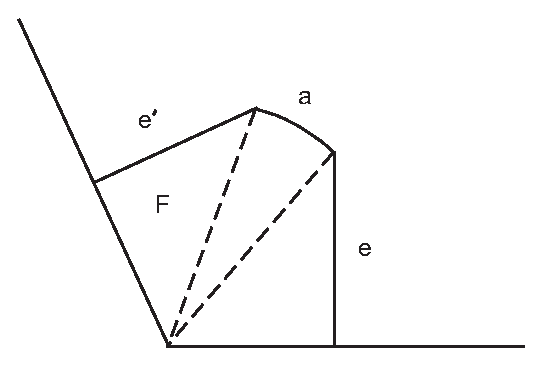
\includegraphics{PS/diag-face.eps}
  \caption{A planar region.}
  \label{fig:face}
\end{figure}

{\bf Case 1. Circumradius of $S$ is less than $\sqrt2$:}  We show
that this case does not occur.  If none of the edges of this
simplex pass through a barrier, then this simplex belongs to
$\CalQ_0'$, a case already considered.  By definition of the
wedges, the edges $\{0,v\}$, $\{0,w\}$, $\{0,w'\}$, $\{v,w\}$, and
$\{v,w'\}$ do not pass through a barrier.  Since five of the six
edges do not pass through a barrier, and since $S$ is formed by
consecutive triangles in the fan around $\{0,v\}$, the sixth does
not pass through a barrier either, by Lemma~\ref{lemma:sixth}.

%This leaves $\{w,w'\}$, which must pass through a barrier
%$T=\{u,u',u''\}$.

%No edge of the barrier $T$ can be $\{0,v\}$ because then $T$ would
%be a triangle in the fan between $w$ and $w'$, which are assumed
%to be consecutive.  No edge of $T$ can pass through a face of $S$
%because its circumradius is less than $\sqrt2$ and
%Lemma~\ref{lemma:no-pass-sqrt2}.  No other edge of $S$ can pass
%through $T$ by Lemma~\ref{lemma:single-enclosed}.  It is now
%apparent that $T$ cannot be placed anywhere at all.  This case
%cannot occur.


{\bf Case 2. Circumradius of $S$ at least $\sqrt2$:} Let
$r\ge\sqrt2$ be the circumradius.   We claim that the edge $e$
cannot extend beyond the wedge through the half plane through
$\{0,v,w'\}$.  In fact, the circumcenter of $\{0,v,w,w'\}$ lies on
the extension (in one direction or the other) of the segment $e$
to a point at distance $r$ from the origin.  If this circumcenter
does not lie in the wedge, then the orientation is negative along
one of the faces $\{0,v,w\}$ or $\{0,v,w'\}$. This face must have
circumradius at least $\sqrt2$, by Lemma~\ref{lemma:sqrt2-chi+},
and this forces the face to be a barrier.  If the orientation is
negative along a barrier, then the simplex $\{0,v,w,w'\}$ is a
simplex in $\CalQ_0$ (Lemmas~\ref{lemma:neg-orient-quad} and
\ref{lemma:neg-orient-tet}). This is contrary to our assumption
above that $\{0,v,w,w'\}$ is not in $\CalQ_0$.




%We observe that the arc marked on a unit sphere coming from a
%barrier is always as least as long as the radius marked on a unit
%sphere coming from a cone $C(u)$.  To see this, we note that the
%arc radius cut out on the unit sphere from the radial projection
%of $u$ to the edge of the cone $C(u)$ is
%$\arc(|u|,\sqrt2,\sqrt2)$. The arc cut out by an edge $\{u,u'\}$
%of a barrier $\{u,u',0\}$ is at least
%$\arc(|u|,\sqrt8,2)\ge\arc(|u|,\sqrt2,\sqrt2)$.  This establishes
%the observation.

These comments show that Figure~\ref{fig:face} correctly
represents the basic shape of $F$, with the understanding that the
edges $e$ and $e'$ may degenerate to a point.  By construction,
every point $x$ in the open convex hull $\{F,0\}$ of $F$ and $0$
lies in $C'(v)\subset \op{VC}(0)$. The convex hull $\{F,0\}$ is
the union of three solids, two Rogers simplices along the
triangles $\{0,v,w\}$ and $\{0,v,w'\}$ respectively, and the conic
solid given by the convex hull of the arc $a$, $v/2$ and $0$. By
Lemmas~\ref{lemma:rogers-app} and \ref{lemma:wedge}, these solids
have density at most $\doct$.

%By Lemma~\ref{lemma:sqrt2-unobstructed}, the origin is not
%obstructed at $x$.  Hence, if $x$ lies in the $V$-cell at $u\ne0$,
%then $|u-x|\le\sqrt2$ and $|x|\le\sqrt2$. This means that $x$ lies
%in the intersection of cones $C(v)\cap C(u)$.

%For there to be a nonempty intersection $\emptyset\ne C(v)\cap
%C(u)$, the circumradius of $\{0,v,u\}$ must be less than $\sqrt2$.
%We consider two cases depending on whether $u$ is some vertex
%$w_j$ (that is, part of the fan).

%Assume the vertex $u=w_j$ is part of the fan.  If $u=w$ or $u=w'$,
%then by construction, no point of $\{F,0\}$ is closer to $u$ than
%to the origin.  (Truncation along the edges $e$ and $e'$
%accomplishes this.) If $u\ne w,w'$, then the parts of $C(v)$ in
%the $V$-cell at $u$ lie in the two wedges alongside the leaf
%$\{0,v,u\}$ of the fan. Thus no such point lies in the wedge in
%question.  Lemma~\ref{lemma:V-cell-local} keeps the $V$-cell from
%leaking past one leaf of the fan to the next.

%Assume that the vertex $u$ is not part of the fan.  By
%construction, we have that the circumradius of $\{0,u,v\}$ is less
%than $\sqrt2$, so that some  edge of $\{0,u,v\}$ crosses a barrier
%$T$ .  The edge that crosses cannot be $\{0,v\}$ because it is too
%short (see Lemma~\ref{lemma:2t0-doesnt-pass-through}).  Let
%$\{u',u''\}\subset \{0,u,v\}$ be the edge passing through $T$.

%{\bf Case-3-b-i. The edge $\{u,v\}$ passes through $T$:} By
%Lemma~\ref{lemma:eta-barrier} at least one-endpoint of $\{v,u\}$
%forms a simplex in $\CalQ_0$ with the barrier, and $0$ is a vertex
%of $T$.  By the observation above, if there is intersection of
%$C(u)$ and $C(v)$, it must be in the convex hull of $T$ and
%$\{u,v\}$.

%If $|v|\le 2t_0$ and $\{T,v\}\not\in\CalQ_0$, then there is not
%overlap in this convex hull by Lemma~\ref{lemma:cone-avoidance}.
%If $\{T,v\}\in\CalQ_0$, then it follows that $\{w,w'\}\subset T$
%and this falls into Case~1, which has already been considered.
%Assume that $|v|\ge 2t_0$. By geometric considerations
%    $$|u-v| \ge \CalE(S(2,2,2,2t_0,2t_0,\sqrt8,2,2,2t_0)  >
%    2.77.$$
%Thus, the circumradius of $\eta(0,u,v)$ is at least
%$\eta(2.51,2.77,2) > \sqrt2$.  This is contrary to the hypothesis
%that $\eta(0,u,v)\le\sqrt2$.  Thus, this case does not occur.

% This means that we have one of
%the situations of Figure~\ref{fig:tricone}. In each case there is
%no overlap between $C(u)$ and $C(v)$, except possibly in points
%over a simplex in $\CalQ_0$.  We have used
%Lemma~\ref{lemma:cone-avoidance}, which separates the cones $C(u)$
%and $C(v)$ from the simplices in $\CalQ_0$. Thus no point of
%$\op{VC}(u)$ meets $\{F,0\}$.

%{\bf Case-3-b-ii. The edge $\{u,0\}$ passes through $T$:}  By
%Lemma~\ref{lemma:eta-barrier}, $v$ is a vertex of $T$, and either
%$\{0,T\}$ or $\{u,T\}$ is a simplex in the $Q$-system.

%Assume $S=\{0,T\}$ is in the $Q$-system.  If $x$ is not in the
%cone over $S$, then Lemma~\ref{lemma:V-cell-local} bounds the
%$V$-cell at $u$ away from $x$.  If $x$ lies in the cone over $S$,
%then $T=\{v,w,w'\}$, where $\{0,v,w\}$ and $\{0,v,w'\}$ are
%consecutive triangles in the flag around $\{0,v\}$.  This
%situation was treated in Case 1.

%Assume that $S=\{u,T\}$ is a simplex in the $Q$-system, and that
%$\{0,T\}$ is not a simplex in the $Q$-system.   Let $H$ be the
%convex hull of $T$, $u$ and $0$. If $x$ lies outside this convex
%hull, then $x$ cannot lie in the interior of both $B(u,\sqrt2)$
%and $B(0,\sqrt2)$. In fact, the shortest path outside $H$ from $0$
%to $u$ has length at least $\sqrt2$ along a face of $\{0,T\}$ and
%length an additional $\sqrt2$ along a face of $\{u,T\}$.

%Lemma~\ref{lemma:sqrt2-unobstructed} implies that $x$ cannot
%belong to $S$.  Assume that $x$ belongs to $H$. Then $x$ lies in
%the convex hull of $\{0,T\}$.  The vertex $u$ is then obstructed
%at $x$ through the barrier $T$.  Thus $x$ does not lie in the
%$V$-cell at $u$.

%This completes the proof of the claim: all points $x$ in the open
%convex hull $\{F,0\}$ of $F$ and $0$ lie in the $V$-cell at $0$.
%To complete the proof, we show that this convex hull has density
%at most $\doct$.



This completes the proof that $\sigma_R(D)$ is never positive on
non-triangular standard regions $R$.  Note that the decomposition
into the parts of cones $C'(v)$ inside a wedge is compatible with
the partition of the unit sphere into standard regions, so that
the estimate holds over each standard region, and not just over
the union of the standard regions.
%
\end{proof}






\begin{lemma}  If $R$ is a standard region that is not a triangle,
and if $\sigma_R(D)=0$, then $(R,D)$ is a quad cluster.  Moreover,
the four corners of $R$ in the quad cluster have height $2$,
forming a square of side $2$.
\end{lemma}

\begin{proof}
To analyze the case of equality, first we note that any truncation
at $1.18$ produces a strict inequality (Lemma~\ref{lemma:cone} is
strict if the volume is nonzero), so that every point must lie
over a simplex in $\CalQ_0'$ or over some $C'(v)$. We have
$\svor(S)<0$ for simplices with circumradius less than $\sqrt2$.
The only simplices in $\CalQ_0$ that produce equality are those
with five edges of length $2$ and a diagonal of length $\sqrt8$.
Any nontrivial arc $a$ produces strict inequality (see
Lemma~\ref{lemma:wedge}, so we must have that $e$ and $e'$ meet at
exactly distance $\sqrt2$ from $0$ and $v$.  Moreover, if $e$ does
not degenerate to a point, the corresponding Rogers simplex gives
strict inequality, unless $\{0,v,w\}$ is an equilateral triangle
with side length $2$.  We conclude that the entire part of the
$V$-cell over the standard region must be assembled from Rogers
simplices $R(1,\eta(2,2,2),\sqrt2)$, and quarters with lengths
$(2,2,2,2,2,\sqrt8)$.  This forces each vertex $v$ of height at
most $2t_0$ to have height $2$.  It forces each pair of triangles
$\{0,v_1,v_2\}$ $\{0,v_2,v_3\}$, that determine consecutive edges
along the boundary of the standard region to meet at right angles:
    $$\dih(0,v_2,v_1,v_3)=0.$$
This forces the object to be a quad cluster of the indicated form.
\end{proof}

We conclude the \chap\ with a proof of the main theorem.  With all
our preparations in place, the proof is short.

\begin{proof} {\bf Theorem~\ref{lemma:local-optimality} (Local
Optimality)} The hypothesis implies that there are $6$ quad clusters
and $8$ quasi-regular tetrahedra at the origin of the decomposition
star. By Lemma~\ref{lemma:1pt}, each quasi-regular tetrahedron
scores at most $1\,\pt$ with equality if and only if the tetrahedron
is regular with edge-length $2$.  By Theorem~\ref{lemma:quad0}, each
quad cluster scores at most $0$, with equality if and only if the
corners of the quad cluster form a square with edge-length $2$ at
distance $2$ from the origin. Thus, $\sigma(D)$ is at most $8\,\pt$.
In the case of equality, there are $12$ vertices at distance $2$
from the origin, forming $8$ equilateral triangles and $6$ squares
(all of edge-length $2$). These conditions are satisfied precisely
when the arrangement is $U_{fcc}$ or $U_{hcp}$ up to a Euclidean
motion.
\end{proof}
}

%%%%%%%%%%%%%%%%%%%%%%%%%%%%%%%%%%%%%%%%%%%%%%%%%%%%
%%%%%%%%%%%%%%%%%%%%%%%%%%%%%%%%%%%%%%%%%%%%%%%%%%%%

\longversion{
    \part{Sphere Packings IV. Detailed Bounds}
    \label{part:bounds}
    %% INTRO SPIV

This paper contains the technical heart of the proof of the Kepler
conjecture.  Its primary purpose is to obtain good bounds on the
score $\sigma_R(D)$ when $R$ is an arbitrary standard region of a
decomposition star $D$.  This is particularly challenging, because
we have no {\it a priori} restrictions on the combinatorial type of
the standard region $R$.  It is not known to be bounded by a simple
polygon.  It is not known to be simply connected. Moreover, there
are multitudes of possible geometrical configurations of upright and
flat quarters, each scored by a different rule.  This paper will
deal with these complexities and will bound the score $\sigma_R(D)$
in a way that depends on a simple numerical invariant $n(R)$ of $R$.
When $R$ is bounded by a simple polygon, the numerical invariant is
simply the number of sides of the polygon. This bound on the score
of a standard region represents the turning point of the proof, in
the sense that it caps the complexity of a contravening
decomposition star, and restrains the combinatorial possibilities.
Later in the proof, it will be instrumental in the complete
enumeration of the plane graphs attached to contravening stars.

The first section will prove a series of approximations for the
score of upright quarters.  The strategy is to limit the number of
geometrical configurations of upright quarters by showing that a
common upper bound (to the scoring function) can be found for quite
disparate geometrical configurations of upright quarters. When a
general upper bound can be found that is independent of the
geometrical details of upright quarters, we say that the upright
quarters can be {\it erased.}  (A precise definition of what it
means to erase an upright quarter appears below.)  There are some
upright quarters that cannot be treated in this manner; and this
adds some complications to the proofs in this paper

The second section states the main result of the paper
(Theorem~\ref{thm:the-main-theorem}).  An initial reduction reduces
the proof to the case that the boundary of the given standard region
is a polygon.  A further argument is presented to reduce the proof
to a convex polygon.

The third section completes the proof of the main theorem.  This
part of the proof relies on a new geometrical decomposition of the
part of a $V$-cell over a standard region. The pieces in this
decomposition are called {\it truncated corner cells}.

A final section in this paper collects miscellaneous further bounds
that will be needed in later parts of the proof of the Kepler
conjecture.

    
\longversion{This paper contains the technical heart of the proof of
the Kepler conjecture.  Its primary purpose is to obtain good bounds
on the score $\sigma_R(D)$ when $R$ is an arbitrary standard region
of a decomposition star $D$.  This is particularly challenging,
because we have no {\it a priori} restrictions on the combinatorial
type of the standard region $R$.  It is not known to be bounded by a
simple polygon.  It is not known to be simply connected. Moreover,
there are multitudes of possible geometrical configurations of
upright and flat quarters, each scored by a different rule.  This
paper will deal with these complexities and will bound the score
$\sigma_R(D)$ in a way that depends on a simple numerical invariant
$n(R)$ of $R$.  When $R$ is bounded by a simple polygon, the
numerical invariant is simply the number of sides of the polygon.
This bound on the score of a standard region represents the turning
point of the proof, in the sense that it caps the complexity of a
contravening decomposition star, and restrains the combinatorial
possibilities.  Later in the proof, it will be instrumental in the
complete enumeration of the plane graphs attached to contravening
stars.}

\longversion{The first section will prove a series of
approximations for the score of upright quarters.  The strategy is
to limit the number of geometrical configurations of upright
quarters by showing that a common upper bound (to the scoring
function) can be found for quite disparate geometrical
configurations of upright quarters.  When a general upper bound
can be found that is independent of the geometrical details of
upright quarters, we say that the upright quarters can be {\it
erased.}  (A precise definition of what it means to erase an
upright quarter appears below.)  There are some upright quarters
that cannot be treated in this manner; and this adds some
complications to the proofs in this paper}

\longversion{The second section states the main result of the
paper (Theorem~\ref{thm:the-main-theorem}).  An initial reduction
reduces the proof to the case that the boundary of the given
standard region is a polygon.  A further argument is presented to
reduce the proof to a convex polygon.}

\longversion{The third section completes the proof of the main
theorem.  This part of the proof relies on a new geometrical
decomposition of the part of a $V$-cell over a standard region.
The pieces in this decomposition are called {\it truncated corner
cells}.}

\longversion{A final section in this paper collects miscellaneous
further bounds that will be needed in later parts of the proof of
the Kepler conjecture.}





\chapter{Upright Quarters}
    \label{sec:upright}
    \oldlabel{3}

\section{Erasing Upright Quarters}
    \oldlabel{3.1}

\begin{definition}
A standard region is said to be {\it exceptional\/} if it is not a
triangle or quadrilateral.  The pair $(D,R)$ consisting of a
decomposition star and an exceptional standard region is said to
be an {\it exceptional cluster}.  The vertices of the packing of
height at most $2t_0$ that are contained in the closed cone over
the standard region are called its {\it corners}.
\end{definition}

Fix an exceptional cluster $R$. Throughout this paper, we assume
that $R$ lies on a star of score at least $\scoregoal$. It is to be
understood, when we say that a standard region does not exist, that
we mean that there exists no such region on any star scoring more
than $\scoregoal$.

In Section~\ref{sec:upright}, we discuss how to eliminate many
cases of upright diagonals. The results are summarized in
Section~\ref{x-3.10}.

If $R$ is a standard region, we write $V_R(t)$ for the
intersection of the local $V$-cell $V_R = \op{VC}(0)\cap C(R)$
with a ball $B(t)$, centered at the origin, of radius $t$.  We
usually take $t=t_0$. If $\{0,v\}$, of length between $2t_0$ and
$2\sqrt{2}$, is not the diagonal of an upright quarter in the
$Q$-system, then $v$ does not affect the truncated cell $V_R(t_0)$
and may be disregarded. For this reason we confine our attention
to upright diagonals that lie along an upright quarter in the
$Q$-system.

%\section{Truncation}
    \oldlabel{3.2}

We say that an upright diagonal $\{0,v\}$ can be {\it erased with
penalty $\pi_0\ge0$}, if we have, in terms of the  decomposition
of \Chap~\ref{sec:fine},
    $$
    \sum_Q\sigma(Q) +\sum_S\sigma(V_S(t_S)) - 4\doct\op{vol}(\delta_P(v))<
        \pi_0+\sum_Q\svor_0(Q) +\sum_S\svor_0(S).
    $$
Here the sum over $Q$ runs over the upright quarters around
$\{0,v\}$. The scores $\sigma(Q)$ are context-dependent (see
Section~\ref{sec:scoring}). The second sum runs over simplices $S$
along $\{0,v\}$ of type $\SC$ in the $\CalS$-system.  We define
their score $\sigma(V_S(t_S))$ as in \Chap~\ref{sec:fine}. Also,
$\delta_P(v)$ is the piece of the decomposition defined in
\Chap~\ref{sec:fine}. The right-hand side is scored by the
truncation function in \Chap~\ref{sec:scoring}
Formula~\ref{eqn:3.7}. When we erase without mention of a penalty,
$\pi_0=0$ is assumed.

If the diagonal can be erased, an upper bound on the score is
obtained by ignoring the upright diagonal and all of the
structures around it coming from the decomposition of
\Chap~\ref{sec:fine}, and switching to the truncation at $t_0$.
Section~\ref{x-3} shows that various vertices can be erased, and
this will greatly reduce the number combinatorial possibilities
for an exceptional cluster.

\section{Contexts}
    \oldlabel{3.3}

Each upright diagonal has a context $\x(p,q)$, with $p$ the number
of anchors and $p-q$ the number of quarters around the diagonal
(Definition~\ref{def:context}). The dihedral angle of a quarter is
less than\footnote{\calc{971555266}} $\pi$, so the context
$\x(2,0)$ is impossible. There is at least one quarter, so $p\ge
q+1$, $p\ge2$.

The context $\x(2,1)$ is treated in Section~\ref{sec:bounds}.
Lemma~\ref{lemma:mixed-vor0} shows that by removing the upright
diagonal, and scoring the surrounding region by a truncated
function $\vor_0$, an upper bound on the score is obtained. In the
remaining contexts, $p\ge3$. We start with contexts satisfying
$p=3$. The context $\x(3,0)$ is to be regarded as two
quasi-regular tetrahedra sharing a face rather than as three
quarters along a diagonal.  In particular, by
Definition~\ref{def:q-system}, the upright quarters do not belong
to the $Q$-system.

We recall that the score of an upright quarter is given by
$$\sigma(Q,v)=(\mu(Q,v)+\mu(Q,\hat v) + \svor_0(Q,v)-\svor_0(Q,\hat v))/2,$$
except in the contexts $\x(2,1)$ and $\x(4,0)$.  Define $\nu(Q)$
to be the right-hand side of this equation.\index{zznu@$\nu$}  The
context $\x(2,1)$ has been treated, and the context $\x(4,0)$ does
not occur in exceptional clusters. Thus, for the remainder of this
\chap, the scoring rule $\sigma(Q)=\nu(Q)$ will be used.

We have several different variants on the score depending on the
truncation, analytic continuation, and so forth.  If $f$ is any of the
functions
    $$\svor_0,\ \svor,\ \Gamma, \ \nu,$$
we set $\tau_{0}$, $\tau_V$, $\tau_\Gamma$,
$\tau_\nu$, respectively,
to
    $$\tau_* = -f(S) +\sol(S)\zeta\pt.$$
We set
    $\tau(S,t) = -\svor(S,t)+\sol(S)\zeta\pt$.
The family of functions $\tau_*$ measure what is squandered by a
simplex.  We say that $Q$ has {\it compression type\/} or {\it
Voronoi type\/} according to the scoring of $\mu(Q)$.  (See
Section~\ref{sec:rules}.)

Crowns and anchor correction terms are used in Section~\ref{sec:bounds}
to erase upright quarters.  We imitate those methods here. The functions
$\cro$ and $\anc$ are defined and discussed in Section~\ref{sec:bounds}.
If
    $S=S(y_1,\ldots,y_6)$
is a simplex along $\{0,v\}$, set
    $$\kappa(S(y_1,\ldots,y_6))=\cro(y_1/2)\dih(S)/(2\pi) +
        \anc(y_1,y_2,y_6)+\anc(y_1,y_3,y_5).
    $$
$\kappa(S)$ is a bound on the difference in the score resulting from
truncation around $v$. Assume that $S$ is the simplex formed by $\{0,v\}$
and two consecutive anchors around $\{0,v\}$. Assume further that the
circumradius of $S$ is at least $\eta_0(y_1/2)$.  Then we have
    $$\kappa(S) = -4\doct \op{vol}(\delta_P(W^e)),$$
where $W^e$ is the extended wedge constructed in
Section~\ref{sec:deltaP}. To see this, it is a matter of interpreting
the terms in $\kappa$. The function {\it crown\/} enters the volume
through the region over the spherical cap $D_0$ of
Section~\ref{sec:deltaP}, lying outside $B(t_0)$.  By multiplying by
$\dih(S)/(2\pi)$, we select the part of the spherical cap over the
unextended wedge $W$ between the anchors.  The terms {\it anc\/} adjust
for the four Rogers simplices lying above the extension $W^e$.


\section{Three anchors}
    \oldlabel{3.4}

%It is often convenient to use several calculations from the
%inequality archive together as a group.  We define the following
%groups of inequalities $\A_{i}$, for $i=1,\ldots,23$.  The
%inequality archive indicates the grouping of the inequalities.  We
%will say, for instance, that something follows from $\A_{i}$, when
%that group of inequalities is used.

\begin{lemma}
    \oldlabel{3.4.1}
The upright diagonal can be erased in the context $\x(3,2)$.
\end{lemma}


\begin{proof}
Let $v_1$ and $v_2$ be the two anchors of the upright diagonal $\{0,v\}$
along the quarter. Let the third anchor be $v_3$.

Assume first that $|v|\ge 2.696$. If $Q$ is of compression type,
then\footnote{\calc{73974037}} %A10  by $\A_{10}$,
the score is dominated by the truncated
function $\svor_0$.  Assume $Q$ is of Voronoi type. If $|v_1|$,
$|v_2|\le 2.45$, then a calculation\footnote{\calc{764978100}} %A11
gives the result. Take $|v_2|\ge
2.45$.  By symmetry, $|v-v_1|$ or $|v-v_2|\ge 2.45$. The case
$|v-v_1|\ge2.45$ is treated by another calculation.%
\footnote{\calc{764978100}} %A11
We take
$|v-v_2|\ge2.45$. Let $S=\{0,v,v_2,v_3\}$. If $S$ is of type $\SC$,
the result follows.\footnote{\calc{764978100}} %A11
$S$ is of type $\SC$, if and only if $y_4\le 2.77$, (because
    $\eta_{456}\ge\eta(2.45,2,2.77)>\sqrt2$.)
If $S$ is  not of type $\SC$, we argue as follows. The function
$h^2(\eta(2h,2.45,2.45)^{-2}-\eta_0(h)^{-2})$ is a quadratic
polynomial in $h^2$ with negative values for
$2h\in[2.696,2\sqrt{2}]$. From this we find
    $$
    \rad(S)\ge \eta(2h,2.45,2.45) \ge \eta_0(h),\quad\text{where } 2h=|v|,
    $$
and this justifies the use of $\kappa$ (see Section~\ref{x-2.3}
Case (2)). That the truncated function dominates the score now
follows from a calculation.\footnote{\calc{618205535}} %A9

Now assume that $|v|\le 2.696$. If the simplices $\{0,v,v_1,v_3\}$
and $\{0,v,v_2,v_3\}$ are of type $\SC$, the bound follows from a
calculation.\footnote{\calc{73974037}} %A10
\footnote{\calc{764978100}} %A11
%$\A_{10},\A_{11}$.
If say  $S=\{0,v,v_2,v_3\}$ is not of type $\SC$,
then
    $$\rad(S)\ge\sqrt2>  \eta_0(2.696/2)\ge\eta_0(h),$$
justifying the use of $\kappa$. The bound follows from further
calculations.\footnote{\calc{618205535}} %A9
\footnote{\calc{73974037}} %A10
\footnote{\calc{764978100}} %A11
%    $\A_9,\A_{10},\A_{11}$.
($\Gamma+\kappa <\octavor_0$,
etc.)
\end{proof}

\begin{lemma}
    \oldlabel{3.4.2}
    \label{lemma:unerased}
The upright diagonal can be erased in the context $\x(3,1)$, provided
the three anchors do not form a flat quarter at the origin.
\end{lemma}

\begin{proof}
In the absence of a flat quarter, truncate, score, and remove the
vertex $v$ as in the context $\x(3,1)$ of
Lemma~\ref{lemma:mixed-vor0}. If there is a flat quarter, by the
rules of Definition~\ref{def:q-system}, $v$ is enclosed over the
flat quarter. We do nothing further with them for now. This
unerased case appears in the summary at the end of the
section~(\ref{x-3.10}).  See Lemma~\ref{lemma:min0-svor}.
\end{proof}

\section{Six anchors}
    \oldlabel{3.5}

\begin{lemma}  An upright diagonal has at most five anchors.
\end{lemma}

\begin{proof}
The proof relies on constants and inequalities from two
calculations.\footnote{\calc{729988292}} %A3
\footnote{\calc{83777706}} %A8
%$\A_3$ and $\A_8$.
If between two anchors there is a quarter, then the angle is
greater than $0.956$, but if there is not,  the angle is greater than
$1.23$.  So if there are $k$ quarters and at least six anchors, they
squander more than
    $$ k (1.01104) - [2\pi-(6-k)1.23]0.78701 > \squander,$$
for $k\ge0$.
\end{proof}

\section{Anchored simplices}
    \oldlabel{3.6}
    \label{sec:anchored-simplex}

Let $\{0,v\}$ be an upright diagonal, and let
$v_1,v_2,\ldots,v_k=v_1$ be its anchors, ordered cyclically around
$\{0,v\}$.  This cyclic order gives dihedral angles between
consecutive anchors around the upright diagonal. We define the
dihedral angles so that their sum is $2\pi$, even though this will
lead us to depart from our usual conventions by assigning a
dihedral angle greater than $\pi$ when all the anchors are
concentrated in some half-space bounded by a plane through
$\{0,v\}$. When the dihedral angle of $S=\{0,v,v_i,v_{i+1}\}$ is at
most $\pi$, we say that $S$ is an {\it anchored simplex\/} if
$|v_i-v_{i+1}|\le3.2$. (The constant $3.2$ appears throughout this
\chap.) All upright quarters are anchored simplices. If an upright
diagonal is completely surrounded by anchored simplices, the
upright diagonal is sometimes called a {\it loop}. If
$|v_i-v_{i+1}|>3.2$ and the angle is less than $\pi$, we say there
is a {\it large gap\/} around $\{0,v\}$ between $v_i$ and $v_{i+1}$.

To understand how anchored simplices overlap we need a bound satisfied
by vertices enclosed over an anchored simplex.

\begin{lemma}
    \label{lemma:anc-simplex-not-enc}
A vertex $w$ of height between 2 and $2\sqrt{2}$, enclosed in the cone
over an anchored simplex $\{0,v,v_1,v_2\}$ with diagonal $\{0,v\}$ satisfies
$|w-v|\le 2t_0$. In particular, if $|w|\le 2t_0$, then $w$ is an anchor.
\end{lemma}

\begin{proof}  As in Lemma~\ref{lemma:v-interior}, the vertex $w$ cannot lie inside the anchored
simplex.  If $|v_1-v_2|\le 2\sqrt{2}$, the result follows from
Lemma~\ref{lemma:neg-orient-quad}. In fact, if $|w|\le 2\sqrt{2}$,
the Voronoi cells at $0$ and $w$ meet, so that
Lemma~\ref{lemma:neg-orient-quad} forces $\{0,v_1,v_2,w\}$ to be a
quarter. (This observation gives a second proof of
Lemma~\ref{lemma:pass-makes-quarter}.)

Assume that a figure exists with $|v_1-v_2|>2\sqrt{2}$. Suppose for a
contradiction that $|v-w|>2t_0$.    Pivot $v_1$ around $\{0,v_2\}$ until
$|v-v_1|=2t_0$ and $v_2$ around $\{0,v_1\}$ until $|v-v_2|=2t_0$.  Rescale
$w$ so that $|w|=2\sqrt{2}$. Set $x = |v_1-v_2|$. If, through geometric
considerations, $w$ is not deformed into the plane of $\{0,v_2,v_1\}$,
then we are left with the one-dimensional family $|w'|=|w'-w|=2$, for
$w'=v_2,v_1$, $|v-w|=|v|=|v_1-v|=|v_2-v|=2t_0$, depending on  $x$. This
gives a contradiction
    $$
    \begin{array}{lll}
        \pi &\ge \dih(v_2,v_1,0,v) + \dih(v_2,v_1,v,w)\\
        &= 2\dih(S(x,2,2t_0,2t_0,2t_0,2))
         > \pi,
    \end{array}
    $$
for $x>2\sqrt{2}$.
(Equality is attained if $x=2\sqrt{2}$.)

Thus, we may assume that $w$ lies in the plane $P=\{0,v_1,v_2\}$. Take the
circle in $P$ at distance $2t_0$ from $v$. The vertices $0$ and $w$ lie
on or outside the circle. The vertices $v_1$ and $v_2$ lie on the
circle, so the diameter is at least $x>2\sqrt{2}$.  The distance from
$v$ to $P$ is less than $x_0= \sqrt{2t_0^2-2}$.  The edge $\{0,w\}$ cannot
pass through the center of the circle, because $|w|$ is less than the
diameter.
%
Reflect $v$ through $P$ to get $v'$.  Then $|v-v'|< 2x_0$. Swapping
$v_1$ and $v_2$ as necessary, we may assume that $w$ is enclosed over
$\{0,v,v',v_2\}$.  The desired bound $|v-w|\le 2t_0$ now follows from
geometric considerations and the contradiction
    $$
    2\sqrt{2}= |w| > {\CalE}(S(2,2t_0,2t_0,2x_0,2t_0,2t_0),2,2t_0,
        2t_0)= 2\sqrt{2}.
    $$
\end{proof}

\begin{corollary}
A vertex of height at most $2t_0$ is never enclosed over an anchored
simplex.
\end{corollary}

\begin{proof}  If so, it would be an anchor to the upright diagonal, contrary to
the assumption that the anchored simplex is formed by consecutive
anchors.
\end{proof}


\section{Anchored simplices do not overlap}
    \oldlabel{3.7}



\begin{definition}\index{unconfined@3-unconfined}
 \index{crowded4@3-crowded}\index{crowded3@4-crowded}
% Def'n copied from linprog.tex
Consider an upright diagonal that is not a loop. Let $R$ be the
standard region that contains the upright diagonal and its
surrounding quarters.  Assume we are in the context $(4,1)$ or
$(5,1)$.  In the context $(4,1)$, suppose that there does not
exist a plane through the upright diagonal such that all three
quarters lie in the same half-space bounded by the plane. Then we
say that the context is {\it $3$-unconfined}. If such a plane
exists, we say that the context is $3$-crowded. We call the
context $(5,1)$ a $4$-crowded upright diagonal.
Sections~\ref{x-3.4} and \ref{x-3.5} reduce everything to contexts
with $4$ or $5$ anchors around each vertex.  If there are $5$
anchors, Lemma~\ref{x-3.8.1} (and Remark~\ref{rem:2gap}) show that
we can assume at most one large gap.
 This gives contexts $(5,0)$ and $(5,1)$.  If there are $4$ anchors,
 then Lemma~\ref{x-3.9.1} will dismiss all contexts except $(4,0)$ and
 $(4,1)$.
Thus, every upright diagonal is exactly one of the following: a
loop, $3$-unconfined, $3$-crowded, or $4$-crowded.
%\def\Sfour{{{\cal\mathbf S}_4^+}}  --> $4$-crowded upright diagonal
%\def\Sminus{{{\cal\mathbf S}_3^-}} --> $3$-crowded upright diagonal
%\def\Splus{{{\cal\mathbf S}_3^+}}  --> $3$-unconfined upright diagonal
\end{definition}

\begin{definition} \index{zzDelta@$\Delta$}  The Cayley-Menger determinant
expresses the volume of a simplex $S(y1,\ldots,y_6)$ in the form
$\sqrt{\Delta(x_1,\ldots,x_6)}/12$, where $x_i = y_i^2$, and
$\Delta$ is a polynomial with integer coefficients.  The
polynomial $\Delta$ will be used frequently.
\end{definition}

This lemma is a consequence of the two others that follow. The
context of the lemma is the set of anchored simplices that have
not been erased by previous reductions.

\begin{lemma}
    \label{lemma:anchor-no-overlap}
Anchored simplices do not overlap.
\end{lemma}

The remaining contexts have four or  five anchors. Let $w$ and the
anchored simplex $S=\{0,v,v_1,v_2\}$ be as in Section~\ref{x-3.6}.
Our object is to describe the local geometry when an upright
diagonal is enclosed over an anchored simplex. If $|v_1-v_2|\le
2\sqrt{2}$, we have seen in Lemma~\ref{lemma:double-face} that
there can be no enclosed upright diagonal with $\ge 4$ anchors
over the anchored simplex $S$.

Assume  $|v_1-v_2|>2\sqrt{2}$. Let $w_1,\ldots,w_k$, $k\ge4$, be the
anchors of $\{0,w\}$, indexed consecutively. The anchors of $\{0,w\}$ do not
lie in $C(S)$, and the triangles $\{0,w,w_i\}$ and $\{0,v,v_j\}$ do not
overlap. Thus, the plane $\{0,v_1,v_2\}$ separates $w$ from
$\{w_1,\ldots,w_k\}$. Set $S_i=\{0,w,w_i,w_{i+1}\}$.
By a calculation\footnote{\calc{83777706}} %A8
%$\A_8$,
    $$\pi\ge \dih(S_1)+\cdots+\dih(S_{k-1})\ge (k-1)0.956.$$

Thus, $k=4$. The common upright diagonal  of the three simplices
$\{S_i\}$ is {\it $3$-crowded}.  We claim that
$\{v_1,v_2\}=\{w_1,w_4\}$. Suppose to the contrary that, after
reindexing as necessary, $S_0=\{0,w,w_1,v_1\}$ is a simplex, with
$v_1\ne w_1$, that does not overlap $S_1,\ldots,S_3$. Then $\pi\ge
\dih(S_0)+\cdots+\dih(S_3)$. So
    $0.28\ge \pi-3(0.956)\ge \dih(S_0)$.
A calculation\footnote{\calc{83777706}} %A8
now implies that $|w-v_1|\ge 2\sqrt{2}$.

Assume that $\{0,w,v_1,v_2\}$ are coplanar.  Disregard the other vertices.
We minimize $|v_1-v_2|$ when
    $$|w|=2\sqrt{2},\quad |v_2|=|v_1|=|w-v_2|=2,\quad |w-v_1|=2\sqrt{2}.$$
This implies
    $3.2\ge|v_1-v_2|\ge x$,
where $x$ is the largest positive root of the polynomial
$\Delta(8,4,4,x^2,4,8)$. But $x\approx 3.36$, a contradiction.

Since $\{0,w,v_1,v_2\}$ cannot be coplanar vertices, geometric
considerations apply and
    $$
    2\sqrt{2}\ge |w| \ge {\CalE}(S(2,2,2,2,2,3.2),2\sqrt{2},2,2)>2\sqrt{2}.
    $$
This contradiction establishes that $v_1=w_1$.

\begin{lemma}
Around a $3$-crowded upright diagonal, all of the anchored
simplices are quarters.
\end{lemma}

\begin{proof}  The proof makes use of constants and inequalities from
several different calculations.\footnote{\calc{815492935}} %A2
\footnote{\calc{83777706}} %A8
\footnote{\calc{855294746}} %A12
%$\A_2$, $\A_8$, and $\A_{12}$.
The dihedral angles are at most $\pi-
2(0.956) < 1.23$. This forces $y_4\le 2t_0$, for each simplex $S$.
So they are all quarters.
\end{proof}

\begin{lemma}
    \oldlabel{3.7.1}\label{lemma:3-crowded}
If there is $3$-crowded upright diagonal, then the three anchored
simplices squander more than $0.5606$ and score at most $-0.4339$.
\end{lemma}


\begin{proof}  The proof makes use of constants and inequalities from
several different calculations.\footnote{\calc{815492935}} %A2
\footnote{\calc{83777706}} %A8
\footnote{\calc{855294746}} %A12
%$\A_2$, $\A_8$, and $\A_{12}$.
The three anchored simplices squander at
least
    $$
    3 (1.01104) - \pi (0.78701) > 0.5606.
    $$
The bound on score follows similarly from $\nu<-0.9871+0.80449\dih$.
\end{proof}

\begin{lemma}
    \oldlabel{3.7.2}
If a simplex at a $3$-crowded upright diagonal overlaps an
anchored simplex, the decomposition star does not contravene.
\end{lemma}

\begin{proof}
Suppose that $\{0,v,v_1,v_2\}$ is an anchored simplex that another
anchored simplex overlaps, with $\{0,v\}$ the upright diagonal.  Let
$\{0,w\}$ be a $3$-crowded upright diagonal. We score the two
simplices $S'_i = \{0,v,w,v_i\}$ by truncation at $\sqrt{2}$.
Truncation at $\sqrt{2}$ is justified by face-orientation
arguments or by geometric considerations:
    $$
    \CalE(S(2,2t_0,2t_0,2t_0,2t_0,2t_0),2,2,2)>2\sqrt{2}.
    $$
A calculation\footnote{\calc{855294746}} %A12
gives
%$\A_{12}$,
    $$\tau_V(S'_1,\sqrt{2})+\tau_V(S'_2,\sqrt{2})\ge 2(0.13) +
        0.2(\dih(S'_1)+\dih(S'_2)-\pi) > 0.26.
    $$
Together with the three simplices around the $3$-crowded upright
diagonal that squander at least $0.5606$, we obtain the stated
bound.
\end{proof}



\section{Five anchors}
    \oldlabel{3.8}
    \label{sec:five-anchors}


When there are five anchors of an upright diagonal, each dihedral angle
around the diagonal is at most $2\pi-4(0.956)<\pi$.

\begin{remark}\label{rem:2gap}
There are at most
two large gaps by the calculation\footnote{\calc{83777706}} %A8
    $$3(1.65)+2(0.956)>2\pi.$$
\end{remark}

\begin{lemma}
    \oldlabel{3.8.1}
If an upright diagonal has five anchors with two large
gaps, then the three anchored simplices squander $>\squander$.
\end{lemma}

\begin{proof}
By a calculation,\footnote{\calc{83777706}} %A8 $\A_8$,
the anchored simplices are all quarters,
    $1.23+2(1.65)+2(0.956)>2\pi$.
The dihedral angle is less than $2\pi-2(1.65)$.  The linear programming
bound based on various inequalities\footnote{\calc{729988292}} %A3 $\A_3$
is greater than $0.859>\squander$.
\end{proof}

\begin{definition}\index{masked}
Define a {\it masked\/} flat quarter to be a flat quarter that is not in
the $Q$-system because it overlaps an upright quarter in the $Q$-system.
They can only occur in a very special setting.
\end{definition}

\begin{lemma}
    \oldlabel{3.8.2}
Let $\{0,v\}$ be an upright diagonal with at least four anchors. If
$Q$ is a flat quarter that overlaps an anchored simplex along
$\{0,v\}$, then the vertices of $Q$ are the origin and three
consecutive anchors of $\{0,v\}$.
\end{lemma}

\begin{proof}
For there to be overlap, the diagonal $\{w_1,w_2\}$ of $Q$ must pass
through the face $\{0,v,v_1\}$ formed by some anchor $v_1$  (see
Lemma~\ref{lemma:2t0-doesnt-pass-through}).  By
Lemma~\ref{lemma:pass-anchor}, $w_1$ and $w_2$ are anchors of
$\{0,v\}$. By Lemma~\ref{lemma:double-face}, $w_2,v_1$, and $w_1$
are consecutive anchors. If $v_1$ is a vertex of $Q$ we are done.
Otherwise, let $w_3\ne 0,w_1,w_2$ be the remaining vertex of $Q$.
The edges $\{v,v_1\}$ and $\{v_1,0\}$ do not pass through the face
$\{w_1,w_2,w_3\}$ by Lemma~\ref{lemma:2t0-doesnt-pass-through}.
Likewise, the edges $\{w_2,w_3\}$ and $\{w_3,w_1\}$ do not pass
through the face $\{0,v,v_1\}$. Thus, $v$ is enclosed over the
quarter $Q$.

\was{Since $v$ has at least four anchors it is not part of an
isolated pair (Figure~\ref{fig:diag19}). Thus there is another
quarter $Q'$ adjacent to $Q$ along $\{w_1,w_2\}$. If this quarter
shares the face $\{0,w_1,w_2\}$ with $Q$, we have a quad cluster,
and the four anchors give us a quartered octahedron and the
result. If the quarter $Q'$ shares the face $\{w_1,w_2,w_3\}$ with
$Q$, then by Lemma~\ref{lemma:double-face}, the other vertex of
$Q'$ is $v$. Thus, $w_3$ is an anchor of $v$.}

Let $w_3'\ne w_1,v_1,w_2$ be a fourth anchor of $\{0,v\}$. By
Lemma~\ref{lemma:2t0-doesnt-pass-through}, we have $w_3'=w_3$.
\end{proof}

\begin{corollary} (of proof)
If $v$ is enclosed over a flat quarter, then $\{0,v\}$ has at most four
anchors.
\end{corollary}

When we are unable to erase the upright diagonal with five anchors
and a large gap, we are able to obtain strong bounds on the score.

%When an upright diagonal has four upright quarters in the
%$Q$-system and a large gap around it,  we say that the upright
%diagonal is {\it $4$-crowded}.

\begin{lemma}
    \oldlabel{3.8.3}\label{lemma:4-crowded}
Suppose an upright diagonal in a decomposition star has five
anchors and one large gap. The four anchored simplices score at
most $-0.25$. The four anchored simplices squander at least $0.4$.
If any of the four anchored simplices is not an upright quarter
then the decomposition star does not contravene.
\end{lemma}

\begin{proof}
A list of inequalities\footnote{\calc{815492935}} %A2 $\A_2$
together with\footnote{\calc{83777706}} %A8
$\dih>1.65$ give the bound $-0.25$.
Further inequalities \footnote{\calc{729988292}} %A3 $\A_3$
give the bound $0.4$.  To get the final statement of the lemma, we
again use a series of inequalities.\footnote{\calc{628964355}} %A5
\footnote{\calc{187932932}} %A7
\end{proof}

\begin{corollary}  There is at most one $4$-crowded upright
diagonal in a contravening decomposition star.
\end{corollary}

\begin{proof}  The crown along the large gap,
with the bound of the lemma, gives\footnote{\calc{618205535}} %A9
    $0.4-\kappa \ge 0.4+0.02274$
squandered by the upright quarters around a $4$-crowded upright
diagonal. The rest squanders a positive amount (see
Lemma~\ref{lemma:tau-positive}). If there are two $4$-crowded
upright diagonals, use $2(0.4+0.02274)>\squander$.
\end{proof}

\begin{definition}\index{zzxiG@$\xiG$}\index{zzxiV@$\xiV$}
We set $\xiG = 0.01561$, $\xiV = 0.003521$, $\xiG'=0.00935$,
$\xik=-0.029$, $\xikG = \xik+\xiG = -0.01339$.
\end{definition}

The first two constants appear in calculations%
%$\A_{10}$ and $\A_{11}$ as
\footnote{\calc{73974037}} %A10
\footnote{\calc{764978100}} %A11
as penalties for erasing upright quarters of compression type, and
Voronoi type, respectively. $\xiG'$ is an improved bound on the
penalty for erasing when the upright diagonal is at least $2.57$.
Also, $\xik$ is an upper bound\footnote{\calc{618205535}} %A9
 on $\kappa$, when the
upright diagonal is at most $2.57$.  If the upright diagonal is at
least $2.57$, then we still obtain the bound%
\footnote{\calc{618205535}} %A9
$\xikG =-0.02274+\xiG'$ on the sum of $\kappa$ with the
penalty from erasing an upright quarter.

\section{Four anchors}
    \oldlabel{3.9}

\begin{lemma}
    \oldlabel{3.9.1}
If there are at least two large gaps around an upright diagonal with $4$
anchors, then it can be erased.
\end{lemma}

\begin{proof}
There are at least as many large gaps as upright quarters. Each large
gap drops us by $\xik$ and each quarter lifts us by at most%
\footnote{\calc{618205535}} %A9
\footnote{\calc{73974037}} %A10
\footnote{\calc{764978100}} %A11
$\xiG$. We have $\xikG<0$.
\end{proof}

\begin{remark} \label{remark:2.6}
Let $\{0,v\}$ be an enclosed vertex over a flat quarter. Then
    $$|v|\ge\CalE(2,2,2,2t_0,2t_0,2\sqrt2,2,2,2)>2.6.$$
If an edge of the flat quarter is sufficiently short, say $y_6\le2.2$,
then
    $$|v|\ge\CalE(2,2,2,2.2,2t_0,2\sqrt2,2,2,2)>2.7.$$
The two dihedral angles on the gaps are $>1.65$.  If the two quarters
mask a flat quarter, we use the scoring of \ref{x-3.10}.2.c. We have
$0.0114< -2\xikG$.
\end{remark}


When there is one large gap, we may erase with a penalty $\pi_0=0.008$.

\begin{lemma}
    \oldlabel{3.9.2}
    \label{lemma:0.008}
Let $v$ be an upright diagonal with $4$ anchors.  Assume that there is
one large gap.  The anchored simplices can be erased with penalty
$\pi_0=0.008$. If any of the anchored simplices around $v$ is not an
upright quarter then we can erase with penalty $\pi_0=0.00222$.

Moreover, if there is a flat quarter overlapping an upright quarter,
then (1) or (2) holds.
    \begin{enumerate}
    \item The truncated function $\svor_0$ exceeds the score by at least
    $0.0063$. The diagonal of the flat is at least $2.6$, and the edge
    opposite the diagonal is at least $2.2$.
    \item The truncated function exceeds the score by at least
    $0.0114$.  The diagonal of the flat is at least $2.7$, and the edge
    opposite the diagonal is at most $2.2$.
    \end{enumerate}
\end{lemma}

\begin{definition}
Let a $3$-unconfined upright diagonal be an upright diagonal that
has $4$ anchors and one large gap in a situation where there is no
masked flat quarter.
\end{definition}

\begin{proof}
The constants and inequalities used in this proof can be found in
a series of calculations.%
\footnote{\calc{618205535}} %A9
\footnote{\calc{73974037}} %A10
\footnote{\calc{764978100}} %A11


First we establish the penalty $0.008$. The truncated function
$\svor_0$ is an upper bound on the score of an anchored simplex
that is not a quarter.  By these inequalities, the result follows
if the diagonal satisfies $y_1\ge 2.57$.

Take $y_1\le 2.57$. If any of the upright quarters are of Voronoi
type, the result follows from $(\xikG+\xiG<0.008)$. If the edges
along the large gap are less than $2.25$, the result follows from
$(-0.03883+3\xiG = 0.008)$. If all but one edge along the large
gap are  less than 2.25, the result follows from $(-0.0325 + 2\xiG
+ 0.00928 = 0.008)$.

If there are at least two edges along the large gap of length at
least $2.25$, we consider two cases according to whether they lie
on a common face of an upright quarter.  The same group of
inequalities gives the result. The bound $0.008$ is now fully
established.

\smallskip
Next we prove that we can erase with penalty $0.00222$, when one
of the anchored simplices is not a quarter.  If $|v|\ge2.57$, then
we use
    $$2\xiG + \xiV + \xik \le 0.00935+0.003521 -0.2274\le 0.$$
If $|v|\le2.57$, we use
    $$2(0.01561)-0.029 \le 0.00222.$$

\smallskip
Let $v_1\ldots,v_4$ be the consecutive anchors of
the upright diagonal $\{0,v\}$ with $\{v_1,v_4\}$ the large gap.
Suppose $|v_1-v_3|\le 2\sqrt{2}$.

We claim the upright diagonal $\{0,v\}$ is not enclosed over
$\{0,v_1,v_2,v_3\}$. Assume the contrary.  The edge $\{v_1,v_3\}$ passes
through the face $\{0,v,v_4\}$.  Disregarding the vertex $v_2$, by
geometric considerations, we arrive at the rigid figure
    $$
    \begin{array}{lll}
    |v|&=2\sqrt{2},\ |v_1|=|v_1-v|=|v-v_3|=|v_3|=|v_3-v_4|=2
    \\ |v-v_4|&=|v_4|=2t_0,\ |v_1-v_4|=3.2.
    \end{array}
    $$
The dihedral angles of $\{0,v,v_1,v_4\}$ and $\{0,v,v_3,v_4\}$ are
    $$\dih(S(2\sqrt{2},2,2t_0,3.2,2t_0,2))>2.3,\
    \dih(S(2\sqrt{2},2,2t_0,2,2t_0,2))>1.16\
    $$
The sum is greater than $\pi$, contrary to the claim that the edge
$\{v_1,v_3\}$ passes through the face $\{0,v,v_4\}$.
(This particular conclusion leads to the corollary cited at the
end of the proof.)
Thus, $\{v_1,v_3\}$ passes through $\{0,v,v_2\}$ so that the
simplices $\{0,v,v_1,v_2\}$
and $\{0,v,v_2,v_3\}$ are of Voronoi type.

To complete the proof of the lemma, we show that when
there is a masked flat quarter, either (1) or (2) holds.
Suppose we mask a flat quarter $Q'=\{0,v_1,v_2,v_3\}$.
We have established that $\{v_1,v_3\}$ passes through
the face $\{0,v,v_2\}$.
To establish (1) assume that $|v_2|\ge 2.2$.  The remark
before the lemma gives
    $$|v_1-v_3|\ge \CalE(S(2,2,2,2\sqrt{2},2t_0,2t_0),2,2,2)>2.6.$$
The bound $0.0063$ comes from
    $$\xikG + 2\xiV < -0.0063$$

To establish (2) assume that $|v_2|\le 2.2$. The remark gives
    $$|v_1-v_3|\ge \CalE(S(2,2,2,2\sqrt{2},2.2,2t_0),2,2,2)>2.7.$$
  If the simplex
$\{0,v,v_3,v_4\}$ is of Voronoi type, then $$\xik + 3\xiV  < -0.0114$$
Assume that $\{0,v,v_3,v_4\}$ is of compression type. We have
    $$-0.004131 +\xikG + \xiV \le -0.0114.$$
\end{proof}

\begin{corollary}  (of proof)\quad
If there are four anchors and if the upright diagonal is enclosed over a
flat quarter, then there are four anchored simplices and at least three
quarters around the upright diagonal.
\end{corollary}

\section{Summary}
    \oldlabel{3.10}
    \label{sec:upright-summary}

The following index summarizes the cases of upright quarters that have
been treated in Section~\ref{sec:upright}. If the number of anchors is
the number of anchored simplices (no large gaps), the results appear in
Section~\ref{x-5.11}. Every other possibility has been treated.

    \begin{itemize}
    \item 0,1,2 anchors\hfill Sec.~\ref{x-3.3}
    \item $3$ anchors \hfill Sec.~\ref{x-3.4}
        \begin{itemize}
        \item context $\x(3,0)$
        \item context $\x(3,1)$
        \item context $\x(3,2)$
        \item context $\x(3,3)$
        \end{itemize}
    \item $4$ anchors \hfill Sec.~\ref{x-3.9}
        \begin{itemize}
        \item $0$ gaps (Section~\ref{x-5.11})
        \item $1$ gap
        \item $2$ or more gaps
        \end{itemize}
    \item $5$ anchors \hfill Sec.~\ref{x-3.8}
        \begin{itemize}
        \item $0$ gaps (Section~\ref{x-5.11})
        \item $1$ gap ($4$-crowded)
        \item $2$ or more gaps
        \end{itemize}
    \item $6$ or more anchors \hfill Sec.~\ref{x-3.5}
    \end{itemize}


\smallskip
By truncation and various comparison lemmas, we have entirely eliminated
upright diagonals except when there are between three and five anchors.
We may assume that there is at most one large gap around the upright
diagonal.

\smallskip
1.  Consider an anchored simplex $Q$ around a remaining upright
diagonal. The score of is $\nu(Q)$ if $Q$ is a quarter, the
analytic function $\svor(Q)$ if the simplex is of type $\SC$
(Section~\ref{x-2.5}), and the truncated function $\svor_0(Q)$
otherwise.

\smallskip
2.  Consider a flat quarter $Q$ in an exceptional cluster. An
upper bound on the score is obtained by taking the maximum of all
of the following functions that satisfy the stated conditions on
$Q$.  Let $y_4$ denote the length of the diagonal and $y_1$ be the
length of the opposite edge.

(a)  The function $\mu(Q)$.

(b)  $\svor_0(Q) - 0.0063$, if $y_4\ge 2.6$ and $y_1\ge
2.2$.\hfill
    (Lemma~\ref{lemma:0.008})

(c)  $\svor_0(Q) - 0.0114$, if $y_4\ge 2.7$ and $y_1\le 2.2$.
    \hfill (Lemma~\ref{lemma:0.008})

(d)  $\nu(Q_1)+\nu(Q_2)+\svor_x(S)$, if there is an enclosed
vertex
    $v$ over $Q$ of height between $2t_0$ and $2\sqrt{2}$ that
    partitions the convex hull of $(Q,v)$ into two upright quarters
    $Q_1$, $Q_2$ and a third simplex $S$. Here $\svor_x=\svor$
    if $S$ is of type $\SC$, and $\svor_x=\svor_0$ otherwise.
    \hfill (Lemma~\ref{lemma:unerased})

(e)  $\svor(Q,1.385)$ if the simplex is of type $\SB$
(Section~\ref{x-2.5}).

(f) $\svor_0(Q)$ if the simplex is an isolated quarter with
    $\max(y_2,y_3)\ge2.23$, $y_4\ge2.77$,
    and $\eta_{456}\ge\sqrt2$.

\smallskip
3.   If $S$ is a simplex is of type $\SA$, its score is
$\svor(S)$. (Section~\ref{x-2.5}.)

\smallskip

4.  Everything else is scored by the truncation $\vor_0$.
    Formula~\ref{eqn:3.7} is used on these remaining pieces.
    On top of what is obtained for the standard cluster by summing all
these terms, there is a penalty $\pi_0=0.008$ each time a
$3$-unconfined upright diagonal is erased.

\smallskip
5.  The remaining upright diagonals that are not completely
surrounded by anchored simplices are $3$-unconfined, $3$-crowded,
or $4$-crowded from Section~\ref{x-3.7}, \ref{x-3.8},  and
\ref{x-3.9}.

\section{Some flat quarters}
    \oldlabel{3.11}
    \label{sec:some-flat}


Recall that $\xiV=0.003521$, $\xiG=0.01561$, $\xiG'=0.00935$. They are
the penalties that result from erasing an upright quarter of Voronoi
type, an upright quarter of compression type, and an upright quarter of
compression type with diagonal $\ge2.57$. (See calculations.%
\footnote{\calc{73974037}} %A10
\footnote{\calc{764978100}} %A11)

In the next lemma, we score a flat quarter by any of the functions
on the given domains
     $$\hat\sigma=
        \begin{cases}
            \Gamma,& \eta_{234},\eta_{456}\le\sqrt2,\\
             \svor, &\eta_{234}\ge\sqrt2,\\
            \svor_0, & y_4\ge 2.6, y_1\ge2.2,\\
            \svor_0, & y_4\ge 2.7,\\
            \svor_0,& \eta_{456}\ge\sqrt2.
        \end{cases}
    $$

\begin{lemma}
    \oldlabel{3.11.1}
    \label{lemma:hatsigma}
$\hat\sigma$ is an upper bound on the functions in
Section~\ref{x-3.10}.2(a)--(f). That is, each function in
Section~\ref{x-3.10}.2 is dominated by some choice of $\hat\sigma$.
\end{lemma}

\begin{proof}  The only case in doubt is the function of 3.10(d):
$$\nu(Q_1)+\nu(Q_2)+\svor_x(S).$$ This is established by the
following lemma.
\end{proof}


We consider the context $\x(3,1)$ that occurs when two upright
quarters in the $Q$-system lie over a flat quarter. Let $\{0,v\}$ be
the upright diagonal, and assume that $\{0,v_1,v_2,v_3\}$ is the
flat quarter, with diagonal $\{v_2,v_3\}$. Let $\sigma$ denote the
score of the upright quarters and other anchored simplex lying
over the flat quarter.

\begin{lemma}\label{lemma:min0-svor}
    \oldlabel{3.11.2}
    $\sigma\le \min(0,\svor_0)$.
\end{lemma}

\begin{proof}
The bound of $0$ is established in Theorem~\ref{lemma:quad0}.

By a calculation\footnote{\calc{855677395}}, if $|v|\ge 2.69$,
then the upright quarters satisfy
    $$\nu < \svor_0 + 0.01 (\pi/2-\dih)$$
so the upright quarters can be erased.  Thus we assume without
loss of generality that $|v|\le 2.69$.

We have
    $$|v|\ge\CalE(S(2,2,2,2t_0 ,2t_0 ,2\sqrt2),2,2,2)>2.6.$$
If $|v_1-v_2|\le 2.1$,  or $|v_1-v_3|\le 2.1$, then
    $$|v|\ge \CalE(S(2,2,2,2.1,2t_0 ,2\sqrt2),2,2,2)>2.72,$$
contrary to assumption.  So take $|v_1-v_2|\ge 2.1$ and
$|v_1-v_3|\ge2.1$. Under these conditions we have the interval
calculation\footnote{\calc{148776243}} %A13
  $\nu(Q) < \svor_0(Q)$ where $Q$ is the upright quarter.
\end{proof}

\begin{remark}
\label{remark:3rd-quarter} If we have an upright diagonal enclosed
over a masked flat quarter in the context $\x(4,1)$, then there
are $3$ upright quarters.  By the same argument as in the lemma,
the two quarters over the masked flat quarter score $\le\svor_0$.
The third quarter can be erased with penalty $\xiV$.
\end{remark}

Define the {\it central vertex\/} $v$ of a flat quarter to be the
vertex for which $\{0,v\}$ is the edge opposite the diagonal.


\begin{lemma}
    \oldlabel{3.11.3}
$\mu < \svor_0 +0.0268$ for all flat quarters. If the central
vertex has height $\le2.17$, then $\mu<\svor_0+0.02$.
\end{lemma}

\begin{proof}
This is an interval calculation.\footnote{\calc{148776243}} %A13
\end{proof}


We  measure what is squandered by a flat quarter by $\hat\tau =
\sol\zeta\pt - \hat\sigma$.

\begin{lemma}\label{lemma:1.32}
    \oldlabel{3.11.4}
Let $v$ be a corner of an exceptional cluster at which the
dihedral angle is at most $1.32$. Then the vertex $v$ is the
central vertex of a flat quarter $Q$ in the exceptional region.
Moreover, $\hat\tau(Q)>3.07\,\pt$. If $\hat\sigma=\svor_0$ (and if
$\eta_{456}\ge\sqrt2$), we may use the stronger constant
$\tau_0(Q)> 3.07\,\pt+\xi_V+2\xiG'$.
\end{lemma}


\begin{proof} Let $S=S(y_1,\ldots,y_6)$ be the simplex inside the exceptional
cluster centered at $v$, with $y_1=|v|$. The inequality $\dih\le 1.32$
gives the interval calculation $y_4\le 2\sqrt{2}$, so $S$ is a quarter.
The result now follows by
interval arithmetic.\footnote{\calc{148776243}} %A13
\end{proof}


\chapter{Bounds in Exceptional Regions}
    \oldlabel{4}
    \label{sec:BER}

%\section{Positivity}
%    \oldlabel{4.1}





\section{The main theorem}
    \label{sec:the-main-theorem}
    \oldlabel{4.4}

Let $(R,D)$ be a standard cluster. Let $U$ be the set of corners,
that is, the set of vertices in the cone over $R$ that have height
at most $2t_0$.  Consider the set $E$ of edges of length at most
$2t_0$ between vertices of $U$. We attach a multiplicity to each
edge. We let the multiplicity be $2$ when the edge projects
radially to the interior of the standard region, and $0$ when the
edge projects radially to the complement of the standard region.
The other edges, those bounding the standard region, are counted
with multiplicity $1$.

Let $n_1$ be the number of edges in $E$, counted with multiplicities.
Let $c$ be the number of classes of vertices under the equivalence
relation $v\sim v'$ if there is a sequence of edges in $E$ from $v$ to
$v'$. Let $n(R)=n_1+2(c-1)$. If the standard region under $R$ is a
polygon, then $n(R)$ is the number of sides.

\begin{theorem}
    \label{thm:the-main-theorem}
    Let $D$ be a contravening decomposition star.
$\tau_R(D) > t_n$, where $n=n(R)$ and
    $$
    \begin{array}{lll}
    t_4&=0.1317,\quad t_5=0.27113,\quad
    t_6=0.41056,\\
    t_7&=0.54999,\quad t_8=0.6045.
    \end{array}
    $$
The decomposition star scores less than $8\,\pt$, if $n(R)\ge 9$,
for some standard cluster $R$. The scores satisfy
$\sigma_R(D)<s_n$, for $5\le n\le 8$, where
    $$
    s_5=-0.05704,\quad s_6=-0.11408,\quad
    s_7=-0.17112,\quad s_8=-0.22816.
    $$
\end{theorem}

Sometimes, it is convenient to calculate these bounds as a multiple
of $\pt$.  We have
    $$
    \begin{array}{lll}
    t_4&>2.378\,\pt,\quad t_5>4.896\,\pt,\quad
    t_6>7.414\,\pt,\\
    t_7&>9.932\,\pt,\quad
    t_8>10.916\,\pt.
    \end{array}
    $$
    %
    $$
    s_5 < -1.03\,\pt,\quad s_6<-2.06\,\pt,\quad
    s_7<-3.09\,\pt,\quad s_8<-4.12\,\pt.
    $$




\begin{corollary}
    \label{cor:std-aggregate-list}
Every standard region is a either a polygon or one shown in
Figure~\ref{fig:std-aggregates}
\end{corollary}


%\gram|2.2||diag7.1.ps|
%\gram|0.5||SAMF/samfigp20.eps|

\begin{figure}[htb]
  \centering
  \includegraphics{PS/diag7.1.ps}
  \caption{}
  \label{fig:std-aggregates}
\end{figure}


In the cases that are not (simple) polygons, we call the {\it polygonal
hull\/} the polygon obtained by removing the internal edges and
vertices. We have $m(R)\le n(R)$, where the constant $m(R)$ is the
number of sides of the polygonal hull.

\begin{proof}
By the theorem, if the standard region is not a polygon, then $8\ge
n_1\ge m\ge 5$. (Quad clusters and quasi-regular tetrahedra have no
enclosed vertices. See Lemma~\ref{lemma:no-enclosed-tri} and
Lemma~\ref{lemma:at-most-one-negative}.) If $c>1$, then $8\ge
n=n_1+2(c-1)\ge 5+2(c-1)$, so $c=2$, and $n_1=5,6$ (frames $2$ and $5$
of the figure).

Now take $c=1$.    Then $8\ge n\ge 5+(n-m)$, so $n-m\le 3$.  If $n-m=3$,
we get frame $3$. If $n-m=2$, we have $8\ge m+2\ge 5+2$, so $m=5,6$
(frames $1$, $4$).

But $n-m=1$ cannot occur, because a single edge that does not bound the
polygonal hull has even multiplicity.  Finally, if $n-m=0$, we have a
polygon.
\end{proof}

\begin{corollary} \label{lemma:70}
If the type of a vertex of a decomposition star is $(7,0)$, then
it does not contravene.
\end{corollary}

\begin{proof} By Theorem~\ref{thm:the-main-theorem},
if there is a non-triangular region, we have
    $$\tau(D)\ge\tlp(7,0)+t_4>\squander.$$
Assume that all standard regions are triangular.  If there is a
vertex that does not lie on one of $7$ triangles, we have by
Lemma~\ref{lemma:pq}:
    $$\tau(D)\ge\tlp(7,0)+0.55\,\pt>\squander.$$
Thus, all vertices lie on one of the $7$ triangles.  The
complement of these seven triangles is a region triangulation by
$5$ standard regions.  There is some vertex of these $5$ that does
not lie on any of the other $4$ standard regions in the
complement.  That vertex has type $(3,0)$, which is contrary to
Lemma~\ref{lemma:pq-impossible}.
%By the results of Part I, which
%treats the case in which all standard regions are triangles, we
%may assume that the star has at least one quadrilateral.  We then
%have $\tau(D)\ge\tlp(7,0) + t_4
%>\squander$.  The result follows.
\end{proof}

\section{Nonagons}
    \label{sec:nonagon}
    \oldlabel{4.6}

A few additional comments are needed to eliminate $n=9$ and $10$,
even after the bounds $t_9$, $t_{10}$ are established.

\begin{lemma} \label{lemma:s9-t9}
Let $F$ be a set of one or more standard regions bounded by a
simple polygon with at most $9$ edges.  Assume  that
    $$\sigma_F(D) \le s_9\quad\text{and }\tau_F(D)\ge t_9,$$
where $s_9=-0.1972$ and $t_9=0.6978$.  Then $D$ does not
contravene.
\end{lemma}

\begin{proof}
Suppose that $n=9$, and that $R$ squanders at least $t_9$ and
scores less than $s_9$.  This bound is already sufficient to
conclude that there are no other standard clusters except
quasi-regular tetrahedra ($t_9+t_4>\squander$). There are no
vertices of type $(4,0)$ or $(6,0)$: $t_9+4.14\,\pt>\squander$ by
Lemma~\ref{lemma:pq}.   So all vertices not over the exceptional
cluster are of type $(5,0)$. Suppose that there are $\ell$
vertices of type $(5,0)$. The polygonal hull of $R$ has $m\le 9$
edges. There are $m-2+2\ell$ quasi-regular tetrahedra. If $\ell\le
3$, then by Lemma~\ref{lemma:0.55}, the score is less than
    $$s_9+ (m-2+2\ell)\,\pt -0.48 \ell\,\pt < \scoregoal.$$
If on the other hand, $\ell\ge 4$, the decomposition star
squanders more than
    $$t_9+ 4(0.55)\,\pt > \squander.$$
\end{proof}


The bound $s_9$ will be established as part of the proof of
Theorem~\ref{thm:the-main-theorem}.

The case $n=10$ is similar.  If $\ell=0$, the score is less than
    $(m-2)\,\pt\le \scoregoal$,
because the score of an exceptional cluster is strictly negative,
Theorem~\ref{lemma:quad0}.  If $\ell>0$, we squander at least
    $t_{10}+ 0.55\,\pt > \squander$ (Lemma~\ref{lemma:0.55}).


\section{Distinguished edge conditions}
    \oldlabel{4.2}

Take an exceptional cluster.  We prepare the cluster by erasing
upright diagonals, including those that are $3$-unconfined,
$3$-crowded, or $4$-crowded.  The only upright diagonals that we
leave unerased are loops.  When the upright diagonal is erased, we
score with the truncated function $\vor_0$ away from flat
quarters.  Flat quarters are scored with the function
$\hat\sigma$. The exceptional clusters in \Chaps~\ref{x-4} and
\ref{x-5} are assumed to be prepared in this way.


A simplex $S$ is {\it special\/} if the fourth edge has length at
least $2\sqrt{2}$ and at most $3.2$, and the others have length at
most $2t_0$. The fourth edge will be called its diagonal.


We draw a system of edges between vertices.  Each vertex will have
height at most $2t_0$.  The radial projections of the edges to the
unit sphere will divide the standard region into subregions. We
call an edge {\it nonexternal\/} if the radial projection of the
edge lies entirely in the (closed) exceptional region.

\begin{enumerate}
\item Draw all nonexternal edges of length at most $2\sqrt{2}$
except those between nonconsecutive anchors of a remaining upright
diagonal. These edges do not cross (Lemma~\ref{lemma:skew-quad}).
These edges do not cross the edges of anchored simplices
(Lemma~\ref{lemma:qrtet-pair-pass} and
Lemma~\ref{lemma:pass-anchor}).

\item Draw all edges of (remaining) anchored upright simplices
that are opposite the upright diagonal, except when the edge gives
a special simplex. The anchored simplices do not overlap
(Lemma~\ref{lemma:anchor-no-overlap}), so these edges do not
cross. These edges are nonexternal (Lemma~\ref{x-3.6} and
Lemma~\ref{lemma:2t0-doesnt-pass-through}).

\item Draw as many additional nonexternal edges as possible of
length at most $3.2$ subject to not crossing another edge, not
crossing any edge of an anchored simplex, and not being the
diagonal of a special simplex.
\end{enumerate}

We fix once and for all a maximal collection of edges subject to
these constraints. Edges in this collection are called {\it
distinguished\/} edges. The radial projection of the distinguished
edges to the unit sphere gives the bounding edges of regions
called the {\it subregions}.  Each standard region is a union of
subregions. The vertices of height at most $2t_0$ and the vertices
of the remaining upright diagonals are said to form a {\it
subcluster}.


By construction, the special simplices and anchored simplices
around an upright quarter form a subcluster.  Flat quarters in the
$Q$-system, flat quarters of an isolated pair, and simplices of
type $\SA$ and $\SB$ are subclusters.  Other subclusters are
scored by the function $\vor_0$. For these subclusters,
Formula~\ref{eqn:3.7} extends without modification.

\section{Scoring subclusters}
    \oldlabel{4.3}

The terms of Formula~\ref{eqn:3.7} defining
$\vor_{0,P}(D)=\vor_P(D,t_0)$ have a clear geometric
interpretation as quoins, wedges of $t_0$-cones, and solid angles
(see Section~\ref{sec:scoring}). There is a quoin for each Rogers
simplex. There is a somewhat delicate point that arises in
connection with the geometry of subclusters.  It is not true in
general that the Rogers simplices entering into the truncation
$\vor_{0,P}(D)$ of $(P,D)$ lie in the cone over $P$.
Formula~\ref{eqn:3.7} should be viewed as an analytic continuation
that has a nice geometric interpretation when things are nice, and
which always gives the right answer when summed over all the
subclusters in the cluster, but which may exhibit unusual behavior
in general. The following lemma shows that the simple geometric
interpretation of Formula~\ref{eqn:3.7} is valid when the
subregion is not triangular.


\begin{lemma}
    \label{lemma:no-cross}
If a subregion is not a triangle and is not  the subregion
containing the anchored simplices around an upright diagonal, the
cone of arcradius
    $$\psi =\arccos(|v|/(2t_0))$$
centered along $\{0,v\}$, where $v$ is a corner of the subcluster,
does not cross out of the subregion.
\end{lemma}

\begin{proof}
For a contradiction, let $\{v_1,v_2\}$ be a distinguished edge that
the cone crosses. If both edges $\{v,v_1\}$ and $\{v,v_2\}$ have
length less than $2t_0$, there can be no enclosed vertex $w$ of
height at most $2t_0$, unless its distance from $v_1$ and $v_2$ is
less than $2t_0$:
    $$\CalE(S(2,2,2,2t_0,2t_0,3.2),2t_0,2,2)>2t_0.$$
In this case, we can replace $\{v_1,v_2\}$ by an edge of the
subregion closer to $v$, so without loss of generality we may
assume that there are no enclosed vertices when both edges
$\{v,v_1\}$ and $\{v,v_2\}$ have length less than $2t_0$.

The subregion is not a triangle, so $|v-v_1|\ge 2t_0$, or
$|v-v_2|\ge 2t_0$, say $|v-v_1|\ge 2t_0$. Also $|v-v_2|\ge2$.
Pivot so that $|v_1-v_2|=3.2$, $|v-v_1|=2t_0$, $|v-v_2|=2$.  (The
simplex $\{0,v_1,v_2,v\}$ cannot collapse ($\Delta\ne0$) as we
pivot. For more details about why $\Delta\ne0$, see Inequality
\ref{eqn:D>0} in Section~\ref{x-4.8}.)
Then use\footnote{\calc{193836552}} %A1
 $\beta_\psi\le \dih_3$.
\end{proof}

As a consequence, in nonspecial standard regions, the terms in the
Formula~\ref{eqn:3.7} for $\vor_0$ retain their interpretations as
quoins, Rogers simplices, $t_0$-cones, and solid angles, all lying
in the cone over the standard region.


\section{Proof}
    \oldlabel{4.5}

The proof of the theorem occupies the rest of the \chap. The
inequalities for triangular and quadrilateral regions have already
been proved. The bounds on $t_3$, $t_4$, $s_3$, and $s_4$ are
found in Lemma~\ref{lemma:roger0}, Section~\ref{x-3.2},
Lemma~\ref{lemma:1pt}, and Theorem~\ref{lemma:quad0},
respectively. Thus, we may assume throughout the proof that the
standard region is exceptional

We begin with a slightly simplified account of the method of
proof. Set $t_9=0.6978$, $t_{10}= 0.7891$, $t_n=\squander$, for
$n\ge 11$. Set $D(n,k) = t_{n+k} - 0.06585\,k$, for $0\le k\le n$,
and $n+k\ge 4$. This function satisfies
    \begin{equation}
    D(n_1,k_1)+D(n_2,k_2)\ge D(n_1+n_2-2,k_1+k_2-2).
    \label{eqn:D-superadd}
    %\oldlabel{eqn:4.5.1}
    \end{equation}
In fact, this inequality unwinds to $t_r+0.13943\ge t_{r+1}$,
$D(3,2)=0.13943$, and $t_n =(0.06585)2+(n-4)D(3,2)$, for $n=4,5,6,7$.
These hold  by inspection.

Call an edge between two vertices of height at most $2t_0$ {\it long\/}
if it has length greater than $2t_0$. Add the distinguished edges to
break the standard regions into subregions. We say that a subregion has
{\it edge parameters} $(n,k)$ if there are $n$ bounding edges, where $k$
of them are long. (We count edges with multiplicities as in
Section~\ref{sec:the-main-theorem}, if the subregion is not a polygon.)
Combining two subregions of edge parameters $(n_1,k_1)$ and $(n_2,k_2)$
along a long edge $e$ gives a union with edge parameters
$(n_1+n_2-2,k_1+k_2-2)$, where we agree not to count the internal edge
$e$ that no longer bounds. Inequality~\ref{eqn:D-superadd} localizes the
main theorem to what is squandered by subclusters. Suppose we break the
standard cluster into groups of subregions such that if the group has
edge parameters $(n,k)$, it squanders at least $D(n,k)$. Then by
superadditivity (Sec.~\ref{x-4.5}, Formula~\ref{eqn:D-superadd}), the
full standard cluster $R$ must squander $D(n,0) = t_n$, $n=n(R)$, giving
the result.

Similarly, define constants $s_4=0$, $s_9 = -0.1972$, $s_{n}=0$, for
$n\ge10$.  Set $Z(n,k) = s_{n+k}-k\epsilon$, for $(n,k)\ne (3,1)$, and
$Z(3,1)=\epsilon$, where\footnote{Compare \calc{193836552}.} %A1
 $\epsilon=0.00005$. The function
$Z(n,k)$ is subadditive:
    $$Z(n_1,k_1)+Z(n_2,k_2) \le Z(n_1+n_2-2,k_1+k_2-2).$$
In fact, this easily follows from $s_a+s_b\le s_{a+b-4}$, for $a,b\ge
4$, and $\epsilon>0$. It will be enough in the proof of
Theorem~\ref{thm:the-main-theorem} to show that the score of a union of
subregions with edge parameters $(n,k)$ is at most $Z(n,k)$.


\section{Preparation of the standard cluster}
   \label{sec:prep-cluster}
    \oldlabel{4.7}

Fix a standard cluster.  We return to the construction of
subregions and distinguished edges, to describe the penalties.
Take the penalty of $0.008$ for each $3$-unconfined upright
diagonal. Take the penalty $0.03344 = 3\xiG+\xikG$ for $4$-crowded
upright diagonals. Take the penalty $0.04683=3\xiG$ for
$3$-crowded upright diagonals. Set $\maxpi=0.06688$. The penalty
in the next lemma refers to the combined penalty from erasing all
$3$-unconfined, $3$-crowded, and $4$-crowded upright diagonals in
the decomposition star. The upright quarters that completely
surround an upright diagonal (loops) are not erased.

\begin{lemma}
The total penalty from a contravening decomposition star is at
most $\maxpi$.
\end{lemma}

\begin{proof}
Before any upright quarters are erased, each quarter
squanders\footnote{\calc{148776243}} %A13
$>0.033$, so the star squanders $>\squander$ if there
are $\ge25$ quarters.  Assume there are at most $24$ quarters. If
the only penalties are $0.008$, we have $8(0.008)<\maxpi$. If we
have the penalty $0.04683$, there are at most $7$ other quarters
($0.5606+8(0.033)>\squander$) (Lemma~\ref{x-3.7}), and no other
penalties from this type or from $4$-crowded upright diagonals, so
the total penalty is at most $2(0.008)+ 0.04683 < \maxpi$.
Finally, if there is one $4$-crowded upright diagonal, there are
at most $12$ other quarters (Section~\ref{x-3.8}), and erasing
gives the penalty $0.03344+4 (0.008)<\maxpi$.
\end{proof}

The remaining upright diagonals are surrounded by anchored simplices. If
the edge opposite the diagonal in an anchored simplex has length
$\ge2\sqrt2$, then there may be an adjacent special simplex whose
diagonal is that edge.  Section~\ref{x-5.11} will give bounds on the
aggregate of these anchored simplices and special simplices.  In all
other contexts, the upright quarters have been erased with penalties.

Break the standard cluster into subclusters as in Section~\ref{x-4.2}.
If the subregion is a triangle, we refer to the bounds of \ref{x-5.7}.
Sections~\ref{x-4.8}--\ref{x-5.10} give bounds for subregions that are
not triangles in which all the upright quarters have been erased. We
follow the strategy outlined in Section~\ref{x-4.5}, although the
penalties will add certain complications.

We now assume that we have a subcluster without quarters and whose
region is not triangular.  The truncated function $\vor_0$ is an
upper bound on the score.  Penalties are largely disregarded until
Section~\ref{x-5.4}.

We describe a series of deformations of the subcluster that
increase $\vor_{0,P}(D)$ and decrease $\tau_{0,P}(D)$.  These
deformations disregard the broader geometric context of the
subcluster. Consequently, we cannot claim that the deformed
subcluster exists in any decomposition star $D$.  As the
deformation progresses, an edge $\{v_1,v_2\}$, not previously
distinguished, can emerge with the properties of a distinguished
edge. If so, we add it to the collection of distinguished edges,
use it if possible to divide the subcluster into smaller
subclusters, and continue to deform the smaller pieces.  When
triangular regions are obtained, they are set aside until
Section~\ref{x-5.7}.

\section{Reduction to polygons}
    \oldlabel{4.8}

By deformation, we can produce subregions whose boundary is a polygon.
Let $U$ be the set of vertices over the subregion of height $\le2t_0$.
As in Section~\ref{sec:the-main-theorem}, the distinguished edges
partition $U$ into equivalence classes.  Move the vertices in one
equivalence class $U_1$ as a rigid body preserving heights until the
class comes sufficiently close to form a distinguished edge with another
subset. Continue until all the vertices are interconnected by paths of
distinguished edges. $\vor_0$ and $\tau_0$ are unchanged by these
deformations.

If some vertex $v$ is connected to three or more vertices by
distinguished edges, it follows from the connectedness of the open
subregion that there is more than one connected component $U_i$ (by
paths of distinguished edges) of $U\setminus\{v\}$. Move $U_1\cup \{v\}$
rigidly preserving heights and keeping $v$ fixed until a distinguished
edge forms with another component. Continue until the distinguished
edges break the subregions into subregions with polygon boundaries.
Again $\vor_0$ and $\tau_0$ are unchanged.

By the end of Section~\ref{x-4}, we will deform all subregions into
convex polygons.

\begin{remark}
    \label{remark:proof-2}
We will deform in such a way that the edges $\{v_1,v_2\}$ will maintain a
length of at least $2$. The proof that distances of at least $2$ are
maintained is given in Section~\ref{sec:proof-2}.

We will deform in such a way that no vertex  crosses a boundary of the
subregion passing from outside to inside.
\end{remark}

Edge length constraints prevent a vertex from crossing a boundary of the
subregion from the inside to outside.  In fact, if $v$ is to cross the
edge $\{v_1,v_2\}$, the simplex $S=\{0,v_1,v,v_2\}$ attains volume 0.  We
may assume, by the argument of the proof of Lemma~\ref{x-4.3}, that
there are no vertices enclosed over $S$. Because we are assuming that
the subregion is not a triangle, we may assume that $|v-v_1|>2t_0$. We
have $|v|\in[2,2t_0]$.  If $v$ is to cross $\{v_1,v_2\}$, we may assume
that the dihedral angles of $S$ along $\{0,v_1\}$, and $\{0,v_2\}$ are
acute. Under these constraints, by the explicit formulas of
\cite[Sec.~8]{part1}, the vertex $v$ cannot cross out of the subregion
    \begin{equation}
    \Delta(S)\ge \Delta(2t_0^2,4,4,3.2^2,4,2t_0^2)>0.
    %oldtag*
    \label{eqn:D>0}
    \end{equation}

We say that a corner $v_1$ is {\it visible} from another $v_2$ if
$\{v_1,v_2\}$ lies over the subregion.  A deformation may make $v_1$
visible from $v_2$, making it a candidate for a new distinguished edge.
If $|v_1-v_2|\le 3.2$, then as soon as the deformation brings them into
visibility (obstructed until then by some $v$), then
Inequality~\ref{eqn:D>0} shows that $|v_1-v|,|v_2-v|\le2t_0$. So
$v_1,v,v_2$ are consecutive edges on the polygonal boundary, and
$|v_1-v_2|\ge 2\sqrt{4-t_0^2} > \sqrt{8}$. By the distinguished edge
conditions for special simplices, $\{v_1,v_2\}$ is too long to be
distinguished.  In other words, there can be no potentially
distinguished edges hidden behind corners. They are always formed in
full view.

\section{Some deformations}
    \oldlabel{4.9}

\begin{definition}\label{def:concave}
Consider three consecutive corners $v_3,v_1,v_2$ of a subcluster
$R$ such that the dihedral angle of $R$ at $v_1$ is greater than
$\pi$.  We call such an corner {\it concave}.  (If the angle is
less than $\pi$, we call it {\it convex}.)  Similarly, the angle
of a subregion is said to be convex or concave depending on
whether it is less than or greater than $\pi$.
\index{concave}\index{convex}
\end{definition}

Let
    $S=S(y_1,\ldots,y_6)=\{0,v_1,v_2,v_3\}$, $y_i=|v_i|$.
Suppose that $y_6>y_5$.  Let $x_i=y_i^2$.

\begin{lemma}
    \oldlabel{4.9.1}
At a concave vertex, $\partial \vor_0/\partial x_5 >0$ and
    $\partial \tau_0/\partial x_5<0$.
\end{lemma}

\begin{proof}
As $x_5$ varies, $\dih_i(S)+\dih_i(R)$ is constant for $i=1,2,3$. The
part of Formula~\ref{eqn:3.7} for $\vor_0$ that depends on $x_5$ can be
written
    $$-B(y_1)\dih(S)-B(y_2)\dih_2(S)-B(y_3)\dih_3(S)-4\doct
        (\quo(R_{135})+\quo(R_{315})),
    $$
where $B(y_i)=A(y_i/2)+\phi_0$, $R_{135}=R(y_1/2,b,t_0)$,
$R_{315}=R(y_3/2,b,t_0)$, $b=\eta(y_1,y_3,y_5)$, and $A(h) =
(1-h/t_0)(\phi(h,t_0)-\phi_0)$. Set $u_{135}=u(x_1,x_3,x_5)$, and
$\Delta_i = \partial \Delta/\partial x_i$. (The notation comes from
\cite[Sec.~8]{part1} and Section~\ref{sec:scoring}.) We have
    $$\frac{\partial \quo(R(a,b,c))}{\partial b} =
        \frac{-a (c^2-b^2)^{3/2}}{3 b (b^2-a^2)^{1/2}}\le 0
    $$
and $\partial b/\partial x_5\ge0$.  Also, $u\ge0$, $\Delta\ge0$ (see
\cite[Sec.~8]{part1}).  So it is enough to show
    $$V_0(S) = u_{135}\Delta^{1/2}
        \frac{\partial}{\partial x_5} (B(y_1)\dih(S)+B(y_2)\dih_2(S)
        + B(y_3)\dih_3(S))< 0.
    $$
By the explicit formulas of \cite[Sec.~8]{part1}, we have
    $$
    V_0(S) = -B(y_1)y_1\Delta_6 + B(y_2)y_2 u_{135} - B(y_3)y_3 \Delta_4.
    $$
For $\tau_0$, we replace $B$ with $B-\zeta\pt$. It is enough to
show that
    $$
    V_1(S) = -(B(y_1)-\zeta\pt)y_1\Delta_6 + (B(y_2)-\zeta\pt)y_2 u_{135} -
        (B(y_3)-\zeta\pt)y_3 \Delta_4<0.
    $$
The lemma now follows from an interval calculation.
%\footnote{\calc{984628285}} %A14 $\A_{14}$.
We note that the polynomials $V_i$
are linear in $x_4$, and $x_6$, and this may be used to reduce the
dimension of the calculation.
\end{proof}

We give a second form of the lemma when the dihedral angle of $R$ is
less than $\pi$, that is, at a convex corner.


\begin{lemma}
    \oldlabel{4.9.2}
At a convex corner, $\partial \vor_0/\partial x_5 <0$ and
    $\partial \tau_0/\partial x_5>0$, if $y_1,y_2,y_3\in[2,2t_0]$,
$\Delta\ge0$, and (i) $y_4\in[2\sqrt{2},3.2]$, $y_5,y_6\in[2,2t_0]$, or
(ii) $y_4\ge 3.2, y_5,y_6\in[2,3.2]$.
\end{lemma}

\begin{proof}
We adapt the proof of the previous lemma.  Now
$\dih_i(S)-\dih_i(R)$ is constant, for $i=1,2,3$, so the signs change.
$\vor_0$ depends on $x_5$ through
$$\sum B(y_i)\dih_i(S) - 4\doct (\quo(R_{135})+\quo(R_{315})).$$
So it is enough to show that
    $$
    V_0 - 4\doct\Delta^{1/2}u_{135}\frac{\partial}{\partial x_5}
    (\quo(R_{135})+\quo(R_{315}))<0.
    $$
Similarly, for $\tau_0$, it is enough to show that
    $$
        V_1 - 4\doct\Delta^{1/2}u_{135}\frac{\partial}{\partial x_5}
    (\quo(R_{135})+\quo(R_{315}))<0.
    $$
By an interval calculation\footnote{\calc{984628285}} %A14
    $$
    \begin{array}{lll}
    -4\doct  u_{135}\frac{\partial\phantom{x}}{\partial x_5}
    (\quo(R_{135})+\quo(R_{315}))&< 0.82,\quad\hbox{on } [2,2t_0]^3,\\
                            &<0.5,\quad\hbox{on }[2,2t_0]^3, y_5\ge2.189.
    \end{array}
    $$
The result now follows from
the inequalities.\footnote{\calc{984628285}} %A14
\end{proof}

Return to the situation of concave corner $v_1$. Let $v_2$, $v_3$ be the
adjacent corners. By increasing $x_5$, the vertex $v_1$ moves away from
every corner $w$ for which $\{v_1,w\}$ lies outside the region.  This
deformation then satisfies the constraint of
Remark~\ref{remark:proof-2}. Stretch the shorter of $\{v_1,v_2\}$,
$\{v_1,v_3\}$ until $|v_1-v_2|=|v_1-v_3|=3.07$ (or until a new
distinguished edge forms, etc.).  Do this at all concave corners.

By stopping at $3.07$, we prevent a corner crossing an edge from
outside-in. Let $w$ be a corner that threatens to cross a
distinguished edge $\{v_1,v_2\}$ as a result of the motion at a
nonconvex vertex.  To say that the crossing of the edge is from
the outside-in implies more precisely that the vertex being moved
is an endpoint, say $v_1$, of the distinguished edge.  At the
moment of crossing the simplex $\{0,v_1,v_2,w\}$ degenerates to a
planar arrangement, with the radial projection of $w$ lying over
the geodesic arc connecting the radial projections of $v_1$ and
$v_2$. To see that the crossing cannot occur, it is enough to note
that the volume of a simplex with opposite edges of lengths at
most $2t_0$ and $3.07$ and other edges at least $2$ cannot be
planar. The extreme case is
    $$\Delta(2^2,2^2,(2t_0)^2,2^2,2^2,3.07^2) > 0.$$

If $|v_1|\ge2.2$, we can continue the deformations even further. We
stretch the shorter of $\{v_1,v_2\}$ and $\{v_1,v_3\}$ until
$|v_1-v_2|=|v_1-v_3|=3.2$ (or until a new distinguished edge forms,
etc.).  Do this at all concave corners $v_1$ for which $|v_1|\ge2.2$. To
see that corners cannot cross an edge from the outside-in, we argue as
in the previous paragraph, but replacing  $3.07$ with $3.2$.  The
extreme case becomes
    $$\Delta(2.2^2,2^2,(2t_0)^2,2^2,2^2,3.2^2) > 0.$$


\section{Truncated corner cells}
    \oldlabel{4.10}

Because of the arguments in the Section~\ref{x-4.9}, we may assume
without loss of generality that we are working with a subregion with the
following properties. If $v$ is a concave vertex and $w$ is not adjacent
to $v$, and yet is visible from $v$, then $|v-w|\ge3.2$. If $v$ is a
concave corner, then $|v-w|\ge3.07$ for both adjacent corners $w$. If
$v$ is a concave corner and $|v|\ge2.2$, then $|v-w|\ge3.2$ for both
adjacent corners $w$. These hypotheses will remain in force through the
end of Section~\ref{x-4}.

Recall from Definition~\ref{def:concave} that we call a spherical
region {\it convex} if its interior angles are all less than
$\pi$. The case where the subregion is a convex triangle will be
treated in Section~\ref{x-5.7}. Hence, we may also assume in
Sections~\ref{x-4.10} through \ref{x-4.13} that the subregion is
not a convex triangle.

We construct a {\it corner cell\/} at each corner.  It depends on a
parameter $\lambda \in [1.6,1.945]$. In all applications, we take
    $\lambda = 1.945 = 3.2-t_0$, $\lambda = 1.815 = 3.07-t_0$, or
    $\lambda = 1.6 = 3.2/2$.

To construct the cell around the corner $v$, place a triangle along
$\{0,v\}$ with sides $|v|$, $t_0$, $\lambda$ (with $\lambda$
opposite the origin). Generate the solid of rotation around the axis
$\{0,v\}$.  Extend to a cone over $0$.  Slice the solid by the
perpendicular bisector of $\{0,v\}$, retaining the part near $0$.
Intersect the solid with a ball of radius $t_0$.   The cones over
the two boundary edges \index{boundary edges} of the subregion at
$v$ make two cuts in the solid.  Remove the slice that lies outside
the cone over the subcluster.  What remains is the corner cell at
$v$ with parameter $\lambda$.

Corner cells at corners separated by a distance less than $2\lambda$ may
overlap.  We define a truncation of the corner cell that has the
property that the {\it truncated corner cells\/} at adjacent corners do
not overlap. Let $\{0,v_i,v_j\}^\perp$ denote the plane perpendicular to
the plane $\{0,v_i,v_j\}$ passing through the origin and the circumcenter
of $\{0,v_i,v_j\}$.

Let $v_1,v_2,v_3$ be consecutive corners of a subcluster. Take the
corner cell with parameter $\lambda$ at the corner $v_2$.  Slice it by
the planes $\{0,v_1,v_2\}^\perp$ and $\{0,v_2,v_3\}^\perp$, and retain the
part along the edge $\{0,v_2\}$. This is the truncated corner cell (tcc).
By construction tccs at adjacent corners are separated by a plane
$(0,\cdot,\cdot)^\perp$. Tccs at nonadjacent corners do not overlap if
the corners are $\ge2\lambda$ apart. Tccs will only be used in
subregions satisfying this condition. It will be shown in
Section~\ref{x-4.12} that tccs lie in the cone over the subregion (for
suitable $\lambda$).


\section{Formulas for Truncated corner cells}
    \oldlabel{4.11}

We will assign a score to truncated corner cells, in such a way that the
score of the subcluster can be estimated from the scores of the corner
cells.

We write $C_0$ for a truncated corner cell.  We write $C_0^u$ for the
corresponding untruncated corner cell.  (Although we call this the
untruncated corner cell to distinguish it from the corner cell, it is
still truncated in the sense that it lies in the ball at the origin of
radius $t_0$.  It is untruncated in the sense that it is not cut by the
planes $(\ldots)^\perp$.)

For any solid body $X$, we define the {\it geometric} truncated
function by
    $$\vor_0^{g}(X) = 4(-\doct \op{vol}(X) + \sol(X)/3)$$
the counterpart for squander
    $$\tau_0^g(X) = \zeta\pt \sol(X) - \vor_0^g(X).$$
The solid angle is to be interpreted as the solid angle of the cone
formed by all rays from the origin through nonzero points of $X$. We may
apply these definitions to obtain formulas for $\vor_0^{g}(C_0)$, and so
forth.

The formula for the score of a truncated corner cell differs slightly
according to the convexity of the corner.  We start with a convex corner
$v$, and let $v_1$, $v$, and $v_2$ be consecutive corners in the
subregion.

Let $S=\{0,v,v_1,v_2\}$ be a simplex with $|v_1-v_2|\ge3.2$. The formula
for the score of a tcc $C_0(S)$ simplifies if the face of $C_0$ cut by
$\{0,v,v_1\}^\perp$ does not meet the face cut by $\{0,v,v_2\}^\perp$. We
make that assumption in this subsection. Set
    $\chi_0(S) =\vor^g_0(C_0(S))$.
(The function $\chi_0$ is unrelated to the function $\chi$ that was
introduced in Definition~\ref{def:chi} to measure the orientation of
faces.)

    $$
    \begin{array}{lll}
        \psi &= \arc(y_1,t_0,\lambda),\quad h=y_1/2,\\
        R'_{126}&=R(y_1/2,\eta_{126},y_1/(2\cos\psi)),
        \quad R_{126}=R(y_1/2,\eta_{126},t_0),\\
        \sol'(y_1,y_2,y_6) &= +\dih(R'_{126})(1-\cos\psi)-\sol(R'_{126}),\\
        \chi_0(S) &= \dih(S)(1-\cos\psi)\phi_0\\
            &\ -\sol'(y_1,y_2,y_6)\phi_0 -\sol'(y_1,y_3,y_5)\phi_0\\
            &\ +A(h)\dih(S)-
                4\doct (\quo(R_{126})+\quo(R_{135})).
    \end{array}
    $$
In the three lines giving the formula for $\chi_0$, the first line
represents the score of the cone before it is cut by the planes
$\{0,v,v_i\}^\perp$ and the perpendicular bisector of $\{0,v\}$. The second
line is the correction resulting from cutting the tcc along the planes
$\{0,v,v_i\}^\perp$. The face of the Rogers simplex $R'_{126}$ lies along
the plane $\{0,v,v_1\}^\perp$.  The third line is the correction from
slicing the tcc with the perpendicular bisector of $\{0,v\}$.  This last
term is the same as the term appearing for a similar reason in the
formula for $\vor_0$ in Formula~\ref{eqn:3.7}. In this formula $R$ is
the usual Rogers simplex and $\quo(R_{ijk})$ is the quoin coming from a
Rogers simplex along the face with edges $(ijk)$.

The formula for the untruncated corner cell is obtained by setting
``$\sol'$'' and ``$\quo$'' to ``$0$'' in the expression for $\chi_0$.
Thus,
    $$
    \vor^g(C_0^u) = \dih(S)[(1-\cos\psi)\phi_0 + A(h)]
    $$
The formula depends only on $\lambda$, the dihedral angle, and the
height $|v|$.  We write $C_0^u = C_0^u(|v|,\dih)$, and suppress
$\lambda$ from the notation. The dependence on $\dih(S)$ is
linear:
    $$
    \tau^g_0(C_0^u(|v|,\dih))= (\dih/\pi)\tau^g_0(C_0^u(|v|,\pi)).
    $$

The dependence of $\chi_0$ on the fourth edge $y_4=|v_1-v_2|$
comes through a term proportional to $\dih(S)$.  Since the
dihedral angle is monotonic in $y_4$, so is $\chi_0$.  Thus, under
the assumption that $|v_1-v_2|\ge3.2$,  we obtain an upper bound
on $\chi_0$ at $y_4=3.2$. Our deformations will fix the lengths of
the other five variables, and monotonicity gives us the sixth.
Thus, the tccs lead to an upper bound on $\vor^g_0$ (and a lower
bound on $\tau^g_0$) that does not require interval arithmetic.


At a concave vertex, the formula is similar.  Replace ``$\dih(S)$''
with $``(2\pi-\dih(S))$'' in the given expression for $\chi_0$.
We add a superscript $-$ to the name of the function at concave
vertices, to denote this modification: $\chi^-_0(C_0)$.

\section{Containment of Truncated corner cells}
    \oldlabel{4.12}

The assumptions made at the beginning of Section~\ref{x-4.10} remain in
force.

\begin{lemma}
    \oldlabel{4.12.1}
Let $v$ be a concave vertex with $|v|\ge2.2$. The truncated
corner cell at $v$ with parameter $\lambda=1.945$ lies in the truncated
$V$-cell over $R$.
\end{lemma}

\begin{proof}
Consider a  corner cell at $v$ and a distinguished edge $\{v_1,v_2\}$
forming the boundary of the subregion. The corner cell with parameter
$\lambda=1.945$ is contained in a cone of arcradius
    $\theta = \arc(2,t_0,\lambda)< 1.21 <\pi/2$
(in terms of the function {\it arc\/} of Section~\ref{x-2.8}). Take two
corners $w_1$, $w_2$, visible from $v$, between which the given bounding
edge appears. (We may have $w_i=v_i$). The two visible edges, $\{v,w_i\}$,
have length $\ge 3.2$. (Recall that the distinguished edges at $v$ have
been deformed to length $3.2$.) They have arc-length at least
$\arc(2t_0,2t_0,3.2)>1.38$. The segment of the distinguished edge
$\{v_1,v_2\}$ visible from $v$ has arc-length at most
$\arc(2,2,3.2)<1.86$.

We check that the corner cell cannot cross the visible portion of
the edge $\{v_1,v_2\}$. Consider the spherical triangle formed by
the edges $\{v,w_1\}$, $\{v,w_2\}$ (extended as needed) and the
visible part of $\{v_1,v_2\}$. Let $C$ be the radial projection of
$v$ and $AB$ be the radial projection of the visible part of
$\{v_1,v_2\}$. Pivot $A$ and $B$ toward $C$ until the edges $AC$ and
$BC$ have arc-length $1.38$.  The perpendicular from $C$ to $AB$
has length at least
    $$\arccos(\cos(1.38)/\cos(1.86/2))>1.21>\theta.$$
This proves that the corner cell lies in the cone over the subregion.
\end{proof}

\begin{lemma}
    \oldlabel{4.12.2}
Let $v$ be a concave vertex. The truncated corner cell at $v$ with
parameter $\lambda=1.815$ lies in the truncated $V$-cell over $R$.
\end{lemma}

\begin{proof}
The proof proceeds along the same lines as the previous lemma, with
slightly different constants. Replace $1.945$ with $1.815$, $1.38$ with
$1.316$, $1.21$ with $1.1$. Replace $3.2$ with $3.07$ in contexts giving
a lower bound to the length of an edge at $v$, and keep it at $3.2$ in
contexts calling for an upper bound on the length of a distinguished
edge. The constant $1.86$ remains unchanged.
\end{proof}

\begin{lemma}
    \oldlabel{4.12.3}
The truncated corner cells with parameter $1.6$ in a subregion do not
overlap.
\end{lemma}

\begin{proof}
We may assume that the corners are not adjacent. If a nonadjacent
corner $w$ is visible from $v$, then $|w-v|\ge3.2$, and an
interior point intersection $p$ is incompatible with the triangle
inequality: $|p-v|\le 1.6$, $|p-w|<1.6$. If $w$ is not visible, we
have a chain $v=v_0,v_1,\ldots,v_r=w$ such that $v_{i+1}$ is
visible from $v_i$. Imagine a taut string inside the subregion
extending from $v$ to $w$. The radial projections of $v_i$ are the
corners of the string's path.   The string bends in an angle
greater than $\pi$ at each $v_i$, so the angle at each
intermediate $v_i$ is greater than $\pi$. That is, they are
concave. Thus, by our deformations $|v_i-v_{i+1}|\ge3.07$. The
string has arc-length at least $r \arc(2t_0,2t_0,3.07)>r (1.316)$.
But the corner cells lie in cones of arcradius
$\arc(2,t_0,\lambda)< 1$. So $2(1.0)>r(1.316)$, or $r=1$.  Thus,
$w$ is visible from $v$.
\end{proof}

\begin{lemma}
    \oldlabel{4.12.4}
The corner cell for $\lambda \le 1.815$ does not overlap the $t_0$-cone
wedge around another corner $w$.
\end{lemma}

\begin{proof}
We take $\lambda=1.815$. As in the previous proof, if there is overlap
along a chain, then
    $$\arc(2,t_0,\lambda) +\arc(2,t_0,t_0) > r \arc(2t_0,2t_0,3.07),$$
and again $r=1$.  So each of the two vertices in question is visible
from the other. But overlap implies $|p-v|\le1.815$ and $|p-w|<t_0$,
forcing the contradiction $|w-v|<3.07$.
\end{proof}

\begin{lemma}
    \oldlabel{4.12.5}
The corner cell for $\lambda \le 1.945$ at a corner $v$ satisfying
$|v|\ge2.2$ does not overlap the $t_0$-cone wedge around another corner
$w$.
\end{lemma}

\begin{proof}
We take $\lambda=1.945$. As in the previous proof, if there is overlap
along a chain, then
    $$\arc(2,t_0,\lambda) +\arc(2,t_0,t_0) > r \arc(2t_0,2t_0,3.2),$$
and again $r=1$.  Then the result follows from
    $$|w-v|\le |p-v|+|p-w| < 1.945 + t_0 = 3.2.$$
\end{proof}

\begin{definition}\index{penalty-free}\index{penalty-inclusive}
(By {\it penalty-free\/} score, we mean the part of the scoring
bound that does not include any of the penalty terms.  We will
sometimes call the full score, including the penalty terms, the
{\it penalty-inclusive\/} score.)
\end{definition}

Lemma~\ref{x-4.3} was stated in the context of a subregion before
deformation, but a cursory inspection of the proof shows that the
geometric conditions required for the proof remain valid by our
deformations. (This assumes that the subregion is not a triangle, which
we assumed at the beginning of Section~\ref{x-4.10}.) In more detail,
there is a solid $CP_0$ contained in the ball of radius of $t_0$ at the
origin, and lying over the cone of the subregion $P$ such that a bound
on the penalty-free subcluster score is $\vor^g_0(CP_0)$ and squander
$\tau^g_0(CP_0)$.


Let $\{y_1,\ldots,y_r\}$ be a decomposition of the subregion into
disjoint regions whose union is $X$. Then if we let $CP_0(y_i)$ denote
the intersection of $CP_0(y_i)$ with the cone over $y_i$, we can write
    $$\tau^g_0(CP_0) =\sum_i \tau^g_0(CP_0(y_i)).$$

These lemmas allow us to express bounds on the score (and squander) of a
subcluster as a sum of terms associated with individual (truncated)
corner cells. By Lemmas~\ref{x-4.12.1} through \ref{x-4.12.5}, these
objects do not overlap under suitable conditions. Moreover, by the
interpretation of terms provided by Section~\ref{x-4.3}, the cones over
these objects do not overlap, when the objects themselves do not. In
other words, under the various conditions, we can take the (truncated)
corner cells to be among the sets $CP_0(y_i)$.

To work a typical example, let us place a truncated corner cell with
parameter $\lambda=1.6$ at each concave corner.  Place a $t_0$-cone
wedge $X_0$ at each convex corner. The cone over each object lies in the
cone over the subregion. By Lemma~\ref{lemma:no-cross} and
Lemma~\ref{lemma:tau-positive} (see the proof), the $t_0$-cone wedge
$X_0$ squanders a positive amount.  The part $P'$ of the subregion
outside all truncated corner cells and outside the $t_0$-cone wedges
squanders
    $$\sol(P')(\zeta\pt-\phi_0) > 0.$$
where $\sol(P')$ is the part of the solid angle of the subregion
lying outside the tccs. Dropping these positive terms, we obtain a
lower bound on the penalty-free squander:
    $$\tau^g_0(CP_0) \ge \sum_{C_0} \tau^g_0(C_0).$$
There is one summand for each concave corner of the subregion.
Other cases proceed similarly.


\section{Convexity}
    \oldlabel{4.13}

\begin{lemma}
    \oldlabel{4.13.1}
There are at most two concave corners.
\end{lemma}


\begin{proof}
Use the parameter $\lambda=1.6$ and place a truncated corner cell $C_0$
at each concave corner $v$. Let $C_0^u(|v|,\dih)$ denote the
corresponding untruncated cell. The Formula of Section~\ref{x-4.11}
gives
    $$
    \tau_0^g(C_0) =
    \tau^g_0(C^u_0(|v|,\dih))
    - \sol'(y_1,y_2,y_6) \phi'_0
    -\sol'(y_1,y_3,y_5)\phi'_0,
    $$
where $\phi'_0 = \zeta\pt-\phi_0 < 0.6671$. (The conditions $y_5\ge3.07$
and $y_6\ge 3.07$ force the faces along the these edges to have
circumradius greater than $t_0$, and this causes the ``$\quo$'' terms in
the formula to be zero.)

By monotonicity in $\dih$, a lower bound on $\tau^g_0(C^u_0)$ is
obtained at $\dih=\pi$. $\tau_0(C^u_0(|v|,\pi))$ is an explicit monotone
decreasing rational function of $|v|\in[2,2t_0]$, which is minimized for
$|v|=2t_0$.  We find
    $$\tau_0(C_0^u(|v|,\dih))\ge\tau_0(C_0^u(2t_0,\pi)) >0.32.$$

The term $\sol'(y_1,y_3,y_5)$ is maximized when $y_3=2t_0$, $y_5=3.07$,
so that $\sol'< 0.017$.  (This was checked with interval arithmetic in
Mathematica.) Thus,
    $$\tau_0(C_0(v))\ge 0.32 - 2(0.017) \phi_0' > 0.297.$$

If there are three or more concave corners, then the penalty-free corner
cells squander at least $3(0.297)$. The penalty is at most $\maxpi$
(Section~\ref{x-4.7}). So the penalty-inclusive squander is more than
    $3(0.297) - \maxpi >\squander$.
\end{proof}

\begin{lemma}
    \oldlabel{4.13.2}
There are no concave corners of height at most $2.2$.
\end{lemma}

\begin{proof}
Suppose there is a corner of height at most $2.2$. Place an
untruncated corner cell $C^u_0(|v|,\dih)$ with parameter $\lambda
=1.815$ at that corner and a $t_0$-cone wedge at every other corner. The
subcluster squanders at least
    $\tau_0(C_0(|v|,\pi))-\maxpi$.
This is an explicit monotone decreasing rational function of one
variable. The penalty-inclusive squander is at least
    $$\tau_0(C^u_0(2t_0,\pi))-\maxpi > \squander.$$
\end{proof}

By the assumptions at the beginning of Section~\ref{x-4.10}, the lemma
implies that each concave corner has distance at least $3.2$ from every
other visible corner.

As in the previous lemma, when $\lambda=1.945$, a lower bound on what is
squandered by the corner cell is obtained for  $|v|=2t_0$, $\dih=\pi$.
The explicit formulas give penalty-free squander $>0.734$. Two disjoint
corner cells give penalty-inclusive squander $>\squander$.  Suppose two
at $v_1,v_2$ overlap.  The lowest bound is obtained when
$|v_1-v_2|=3.2$, the shortest distance possible.

We define a function $f(y_1,y_2)$ that measures what the union of the
overlapping corner cells squander.  Set $y_i = |v_i|$, $\ell=3.2$, and
    $$
    \begin{array}{lll}
    \alpha_1 &= \dih(y_1,t_0,y_2,\lambda,\ell,\lambda),\\
    \alpha_2 &= \dih(y_2,t_0,y_1,\lambda,\ell,\lambda),\\
    \sol &= \sol(y_2,t_0,y_1,\lambda,\ell,\lambda),\\
    \phi_i &= \phi(y_i/2,t_0),\quad i=1,2,\\
    \lambda&=3.2-t_0=1.945,\\
    f(y_1,y_2)&=
    2(\zeta\pt-\phi_0)\sol+
    2\sum_1^2 \alpha_i(1-y_i/(2t_0))(\phi_0-\phi_i)\\
        &\quad +\sum_1^2 \tau_0(C(y_i,\lambda,\pi-2\alpha_i)).
    \end{array}
    $$
An interval calculation\footnote{\calc{984628285}} %A14
gives $f(y_1,y_2)>\squander+\maxpi$, for $y_1,y_2\in[2,2t_0]$.

We conclude that there is at most one concave corner. Let $v$ be such a
corner.  If we push $v$ toward the origin, the solid angle is unchanged
and $\vor_0$ is increased.  Following this by the deformation of
Section~\ref{x-4.9}, we maintain the constraints $|v-w|=3.2$, for
adjacent corners $w$, while moving $v$ toward the origin. Eventually
$|v|=2.2$. This is impossible by Lemma~\ref{x-4.13.2}.

We verify that this deformation preserves the constraint $|v-w|\ge2$,
for all corners $w$ such that $\{v,w\}$ lies entirely outside the
subregion.  If fact,  every corner is visible from $v$, so that the
subregion is star convex at $v$. We leave the details to the reader.

We conclude that all subregions can be deformed into convex polygons.

\section{Proof that Distances Remain at least $2$}
    \label{sec:proof-2}


\begin{remark}
\label{flexremark} In Section~\ref{remark:proof-2}, to allow for
more flexible deformations, we drop all constraints on the lengths
of (undistinguished) edges $\{v_1,v_2\}$ that cross the boundary of
the subregion.  We deform in such a way that the edges $\{v_1,v_2\}$
will maintain a length of at least $2$.
\end{remark}


Recall that we say that a vertex of a subregion is {\it convex\/}
if its angle is less than $\pi$, and otherwise that is {\it
concave}
(Definition~\ref{def:concave}).\index{convex}\index{concave}
%
In general, if $P$ is a subregions and $p_1$ and $p_2$ are two
vertices of $P$, there is a minimal curve joining $p_1$ and $p_2$
inside $P$.  This curve is a finite sequence $e_1,\ldots, e_r$ of
spherical geodesics.  We refer to this sequence as the {\it sequence
of arcs\/} \index{arc!sequence} from $p_1$ to $p_2$. The endpoint of
each spherical arc is a vertex of $P$. All endpoints except possible
$p_1$ and $p_2$ are nonconvex. These endpoints are the radial
projections of corners of $P$: $v_0,v_1,\ldots,v_{r+1}$, with
$p(v_0)=p_1$ and $p(v_{r+1})=p_2$. The vertex $p_1$ is visible from
$p_2$ if and only if $r=1$.


\begin{lemma}\label{dist2}
This deformation of a subregion at a concave corner $v$ maintains
a distance of at least $2$ to every other corner $w$.
\end{lemma}

\begin{proof}
The proof is by contradiction. We may assume that $|v-w|<\sqrt8$.
We may assume that $v$ and $w$ are the first corners to violate
the condition of being at least $2$ apart, so that distances
between other pairs of corners are at least $2$.  A distinguished
edge connects $v$ and $w$, if $w$ is visible from $v$. So assume
that $w$ is not visible.  Let $e(v_1,v_2)$ be the first
distinguished edge crossed by the geodesic arc $g$ from $p(v)$ to
$p(w)$. Let $p_0$ be the intersection of $e(v_1,v_2)$ and $g$. By
construction, the deformation moves $v$ into the subregion, and
the subregion $P$ is concave at the corner $v$, so that the arc
from $p(v)$ to $p(w)$ begins in $P$, then crosses out at
$e(v_1,v_2)$.

Geometric considerations show that $|v_1-v_2|\ge2.91$.  In fact,
geometric considerations show that the shortest possible distance
for $|v_1-v_2|$ under the condition that $|v-w|\le2$ is the length
of the segment passing through the triangle of sides $2,2t_0,2t_0$
with both endpoints at distance exactly two from all three
vertices of the triangle.  This distance is greater than $2.91$.

Let $e_1,\ldots,e_r$ be the sequence of arcs from $p(v)$ to
$p(v_1)$, and let $f_1,\ldots,f_s$ be the sequence of arcs from
$p(v)$ to $p(v_2)$. Since this sequence forms a minimal curve, the
sum of the lengths of $e_i$ is at most the sum of the lengths of
$e(v,p_0)$ and $e(p_0,v_1)$, and the sum of the lengths of $f_i$
is at most the sum of the lengths of $e(v,p_0)$ and $e(p_0,v_2)$.

Note that if $r+s\le4$, then one of the edge-lengths must be at
least $3.2$, for otherwise the sequence of arcs are all
distinguished or diagonals of specials, and this would not permit
the existence of a corner $w$. That is, we can fully enumerate the
corners of the subregion, and each projects radially to an
endpoint in the sequence of arcs, or is a vertex of a special
simplex. None of these corners is separated from $v$ by the plane
$\{0,v_1,v_2\}$.

We have $r+s\le3$ by the following calculations.  Here
$y\in[2,2t_0]$.
    $$5\arc(2t_0,2t_0,2) > \arc(2,2,3.2)+ 2 \arc(2,2,2).$$
    $$3\arc(2t_0,2t_0,2) + \arc(2t_0,y,3.2) > \arc(y,2,3.2) + 2 \arc(2,2,2).$$
    $$3\arc(2t_0,2t_0,2) + \arc(2t_0,y,3.2) > \arc(2,2,3.2) + 2\arc(y,2,2).$$


First we prove the lemma in the special case that the distance
from $v$ to one of the endpoints, say $v_1$, of $\{v_1,v_2\}$ is at
least $3.2$. In this special case, we claim that the constraints
on the edge-lengths creates an impossible geometric configuration.
The constraints are as follows.  There are $5$ points:
$0,v_1,w,v,v_2$. The plane $\{0,v_1,v_2\}$ separates the point $w$
from $v$. The distance constraints are as follows:
    $$2\le |u| \le 2t_0,$$
for $u=v_1,w,v,v_2$, $|v-v_1|\ge 3.2$, $|v-w|\le2$, $|v-v_2|\ge2$,
$|w-v_1|\ge2$, $|w-v_2|\ge2$, $2\le |v_1-v_2|\le 3.2$.

If the segment $\{v,w\}$ passes through the triangle $\{0,v_1,v_2\}$,
then the desired impossibility proof follows by geometric
considerations. Again, if the segment $\{v_1,v_2\}$ passes through
the triangle $\{0,v,w\}$, then the desired impossibility proof
follows by geometric considerations, provided that $\{0,v_1,v_2,w\}$
are not coplanar. Assume for a contradiction that $\{0,v_1,v_2,w\}$
lie in the plane $P$. We move back to the nonplanar case if
$|v_2-v|$ is not $2$ (pivot $v_2$ around $\{0,w\}$ toward $v$), if
$|v_1-v|$ is not $3.2$ (pivot $v_1$ around $\{0,w\}$ toward $v$), if
$|w-v|$ is not $2$ (pivot $w$ around $\{v_1,v_2\}$ away from $v$),
or $v$ is not $2t_0$ (pivot $v$ and $w$ simultaneously preserving
$|w-v|$ around $\{v_1,v_2\}$).  Therefore, we may assume without
loss of generality that $|v_2-v|=2$, $|v_1-v|=3.2$, $|w-v|=2$, and
$|v|=2t_0$.

Let $p$ be the orthogonal projection of $v$ to the plane $P$.  Let
$h=|v-p|$. The distances from $p$ to $u\in P$ is
$f(|v-u|,h)=\sqrt{|v-u|^2-h^2}$. We consider two cases depending
on whether we can find a line in $P$ through $p$ dividing the
plane into a half-plane containing $v_1$, $0$, and $v_2$, or into
a half-plane containing $v_1$, $w$, and $v_2$.  In the first case
we have
\begin{multline}
    0=\arc(|p-v_1|,|p|,|v_1|)+\\
    \arc(|p-v_2|,|p|,|v_2|)-\arc(|p-v_1|,|p-v_2|,|v_1-v_2|)\\
    \ge \arc(f(3.2,h),f(2t_0,h),2)+\\
    \arc(f(2,h),f(2t_0,h),2)-\arc(f(3.2,h),f(2,h),3.2)
\end{multline}

The function $\arc$ is monotonic in the arguments and from this it
follows easily that this function of $h$ is positive on its domain
$0\le h\le \sqrt3$. This is a contradiction. (The upper bound
$\sqrt3$ is determined by the condition that the triangle
$\{w,v_1,v\}$, which is equilateral in the extreme case, exist under
the given edge constraints.) In the second case, we obtain the
related contradiction
\begin{multline}
    0=\arc(|p-v_1|,|p-w|,|v_1-w|)+
    \arc(|p-v_2|,|p-w|,|v_2-w|)-\\
    \arc(|p-v_1|,|p-v_2|,|v_1-v_2|)\\
    \ge \arc(f(3.2,h),f(2,h),2)+\\
    \arc(f(2,h),f(2,h),2)-\arc(f(3.2,h),f(2,h),3.2)
\\>0
\end{multline}

Now assume that the distances from $v$ to the vertices $v_1$ and
$v_2$ are at most $3.2$.

If $r+s=2$, then $v_1$ and $v_2$ are visible from $v$. Thus, they
are distinguished or diagonals of special simplices. As
$\{v_1,v_2\}$ is also distinguished, the corners of $P$ are fully
enumerated: $v$, $v_1$, $v_2$, and the vertices of special
simplices.  Since none of these are $w$, we conclude that $w$ does
not exist in this case.

If $r+s=3$, then say $r=1$ and $s=2$. We have $\{v,v_1\}$ is
distinguished or the diagonal of a special simplex. Let
$p(v),p(u)$ be the endpoints of $f_1$, for some corner $u$. We
have $|u-v_1|\ge\sqrt8$ because $\{u,v_1\}$ is not distinguished,
and $\max(|u-v|,|u-v_1|)\ge3.2$, because otherwise we enumerate
all vertices of $P$ as in the case $r+s=2$, and find that $w$ is
not among them. But now geometric considerations lead to a
contradiction: there does not exist a configuration of five points
$0$, $u$, $v$, $v_1$, $v_2$, with all distances at least $2$
satisfying these constraints. (This can be readily solved by
geometric considerations.)
\end{proof}


\chapter{Convex Polygons}
    \oldlabel{5}

\section{Deformations}
    \oldlabel{5.1}
We divide the bounding edges over the polygon according to length
$[2,2t_0]$, $[2t_0,2\sqrt{2}]$, $[2\sqrt{2},3.2]$. The deformations of
Section~\ref{x-4.9} contract edges to the lower bound of the intervals
($2,2t_0$, or $2\sqrt{2}$) unless a new distinguished edge is formed. By
deforming the polygon, we assume that the bounding edges have length
$2,2t_0$, or $2\sqrt{2}$. (There are a few instances of triangles or
quadrilaterals that do not satisfy the hypotheses needed for the
deformations. These instances will be treated in Sections~\ref{x-5.7}
and \ref{x-5.8}.)

\begin{lemma}
    \oldlabel{5.1.1}
Let $S=S(y_1,\ldots,y_6)$ be a simplex, with $x_i=y_i^2$,
as usual.  Let $y_4\ge 2$, $\Delta\ge0$,
    $y_5,y_6\in\{2,2t_0,2\sqrt{2}\}$.
Fixing all the variables but $x_1$, let $f(x_1)$ be one of the
functions $\svor_0(S)$ or $-\tau_0(S)$. We have $f''(x_1)>0$
whenever $f'(x_1)=0$.
\end{lemma}

\begin{proof} This is an interval calculation.%
\footnote{\calc{311189443}} %A15
\end{proof}

The lemma implies that $f$ does not have an interior point local maximum
for $x_1\in[2^2,2t_0^2]$.  Fix three consecutive corners, $v_0,v_1,v_2$
of the convex polygon, and apply the lemma to the variable $x_1 =
|v_1|^2$ of the simplex $S=\{0,v_0,v_1,v_2\}$. We deform the simplex,
increasing $f$.  If the deformation produces $\Delta(S)=0$, then some
dihedral angle is $\pi$, and the arguments for nonconvex regions bring
us eventually back to the convex situation. Eventually $y_1$ is $2$ or
$2t_0$.  Applying the lemma at each corner, we may assume that the
height of every corner is $2$ or $2t_0$.   (There are a few cases where
the hypotheses of the lemma are not met, and these are discussed in
Sections~\ref{x-5.7} and \ref{x-5.8}.)

\begin{lemma}
    \oldlabel{5.1.2}
    \label{lemma:7-sides}
The convex polygon has at most $7$ sides.
\end{lemma}

\begin{proof}
Since the polygon is convex, its perimeter on the unit sphere is at most
a great circle $2\pi$.  If there are $8$ sides, the perimeter is at
least $8\arc(2t_0,2t_0,2)>2\pi$.
\end{proof}

\section{Truncated corner cells}
    \oldlabel{5.2}

The following lemma justifies using tccs at the corners as an upper
bound on the score (and lower bound on what is squandered). We fix the
truncation parameter at $\lambda=1.6$.

\begin{lemma}
Take a convex subregion that is not a triangle.  Assume edges between
adjacent corners have lengths $\in\{2,2t_0,2\sqrt{2},3.2\}$. Assume
nonadjacent corners are separated by distances $\ge3.2$.  Then the
truncated corner cell at each vertex lies in the cone over the
subregion.
\end{lemma}

\begin{proof}
Place a tcc at $v_1$. For a contradiction, let $\{v_2,v_3\}$ be an edge
that the tcc overlaps.  Assume first that $|v_1-v_i|\ge 2t_0$, $i=2,3$.
Pivot so that $|v_1-v_2|=|v_1-v_3|=2t_0$.    Write
$S(y_1,\ldots,y_6)=\{0,v_1,v_2,v_3\}$. Set $\psi=\arc(y_1,t_0,1.6)$.
A calculation\footnote{\calc{193836552}} %A1
gives $\beta_\psi(y_1,y_2,y_6)<\dih_2(S)$.

Now assume $|v_1-v_2|<2t_0$.  By the hypotheses of the lemma,
$|v_1-v_2|=2$.  If $|v_1-v_3|<3.2$, then $\{0,v_1,v_2,v_3\}$ is
triangular, contrary to hypothesis.  So $|v_1-v_3|\ge3.2$. Pivot so that
$|v_1-v_3|=3.2$. Then\footnote{\calc{193836552}} %A1
    $$\beta_\psi(y_1,y_2,y_6)< \dih_2(S),$$
where $\psi=\arc(y_1,t_0,1.6)$, provided $y_1\in[2.2,2t_0]$. Also, if
$y_1\in[2.2,2t_0]$
    $$\arc(y_1,t_0,1.6)<\arc(y_1,y_2,y_6).$$

If $y_1\le 2.2$, then $\Delta_1\ge0$, so
    $\partial\dih_2/\partial x_3\le 0$.
Set $x_3=2t_0^2$. Also, $\Delta_6\ge0$, so
    $\partial\dih_2/\partial x_4\le0$.
Set $x_4=3.2^2$.

Let $c$ be a point of intersection of the plane $\{0,v_1,v_2\}^\perp$ with
the circle at distance $\lambda=1.6$ from $v_1$ on the sphere centered
at the origin of radius $t_0$.  The angle along $\{0,v_2\}$ between the
planes $\{0,v_2,v_1\}$ and $\{0,v_2,c\}$ is
    $$\dih(R(y_2/2,\eta_{126},y_1/(2\cos\psi))).$$
This angle is less\footnote{\calc{193836552}} %A1
than $\dih_2(S)$. Also, $\Delta_1\ge0$,
$\partial\dih_3/\partial x_2\le0$, so set $x_2=2t_0^2$. Then
$\Delta_5<0$, so $\dih_2>\pi/2$.  This means that $\{0,v_1,v_2\}^\perp$
separates the tcc from the edge $\{v_2,v_3\}$. \end{proof}

\section{Analytic continuation}
    \oldlabel{5.3}

In this subsection we assume that $\lambda=1.6$ and that the
truncated corner cell under consideration lies at a convex vertex.

Assume that the face cut by $\{0,v,v_1\}^\perp$ meets the face cut by
$\{0,v,v_2\}^\perp$.  Let $c_i$ be the point on the plane
$\{0,v,v_i\}^\perp$ satisfying $|c_i-v|=1.6$, $|c_i|=t_0$. (Pick the root
within the wedge between $v_1$ and $v_2$.) The overlap of the two faces
is represented in Figure~\ref{fig:chi-anal-vs-geom}.

\begin{figure}[htb]
  \centering
  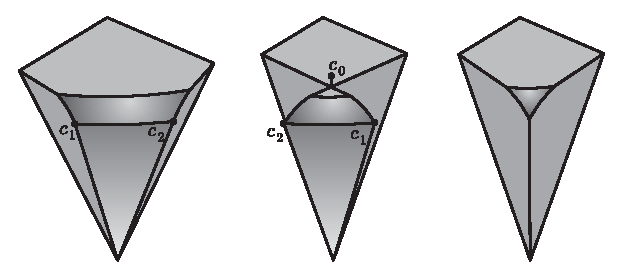
\includegraphics{PS/samfigA54.eps}
  \caption{Different forms of truncated corner cells are shown.  The
  structure
  shown in the middle frame cannot occur.}
  \label{fig:chi-anal-vs-geom}
\end{figure}


We let $c_0$ be the point of height $t_0$ on the intersection of the
planes $\{0,v,v_1\}^\perp$ and $\{0,v,v_2\}^\perp$. We claim that $c_0$ lies
over the truncated spherical region of the tcc, rather than the wedges
of $t_0$-cones or the Rogers simplices along the faces $\{0,v,v_1\}$ and
$\{0,v,v_2\}$.  (This implies that $c_0$ cannot protrude beyond the corner
cell as depicted in the second frame of the figure.) To see the claim,
consider the tcc as a function of $y_4=|v_1-v_2|$. When $y_4$ is
sufficiently large the claim is certainly true.  Contract $y_4$ until
$c_0=c_0(y_4)$ meets the perpendicular bisector of $\{0,v\}$. Then $c_0$
is equidistant from $0,v,v_1$ and $v_2$ so it is the circumcenter of
$\{0,v,v_1,v_2\}$. It has distance $t_0$ from the origin, so the
circumradius is $t_0$. This implies that $y_4\le 2t_0$.

The tcc is defined by the constraints represented in the third frame.
The analytic continuation of the function $\chi_0(S)=\chi_0^\anal(S)$,
defined above, acquires a volume $X$, counted with negative sign, lying
under the spherical triangle $(c_0,c_1,c_2)$. Extending our notation, we
have an analytically defined function $\chi_0^\anal$ and a geometrically
defined function $\chi_0^\geom$,
    $$
    \begin{array}{lll}
    \chi_0^\anal(S) &= \chi_0^\geom(S)-\op{c-vor}_0(X), \text{\ where}\\
    \op{c-vor}_0(X) &= 4(-\doct\op{vol}(X) +\sol(X)/3) = \phi_0\sol(X) <0.
    \end{array}
    $$
So $\chi_0^\anal >\chi_0^\geom$, and we may always use
$\chi_0(S)=\chi_0^\anal(S)$ as an upper bound on the score of a tcc.

For example, with $\lambda=1.6$ and $S = S(2.3,2.3,2.3,2.9,2,2)$, we
have
    $$\chi_0^\anal(S)\approx -0.103981, \quad\chi_0^\geom(S)\approx -0.105102.$$
Or, if $S=S(2,2,2t_0,3.2,2,2t_0)$, then
    $$\chi_0^\anal(S)\approx -0.0718957, \quad
    \chi_0^\geom(S)\approx -0.0726143.$$


\section{Penalties}
    \oldlabel{5.4}
    \label{sec:penalty1}

In Section~\ref{x-4.7}, we determined the bound of
$\maxpi=0.06688$ on penalties. In this section, we give a more
thorough treatment of penalties. Until now a penalty has been
associated with a given standard region, but by taking the worst
case on each subregion, we can move the penalties to the level of
subregions.   Roughly, each subregion should incur the penalties
from the upright quarters that were erased along edges of that
subregion.  Each upright quarter of the original standard region
is attached at an edge between adjacent corners of the standard
cluster. The edges have lengths between $2$ and $2t_0$.  The
deformations shrink the edges to length $2$.  We attach the
penalty from the upright quarter to this edge of this subregion.
In general, we divide the penalty evenly among the upright
quarters along a common diagonal, without trying to determine a
more detailed accounting. For example, the penalty $0.008$ in
Lemma~\ref{lemma:0.008} comes from three upright quarters.  Thus,
we give each of three edges a penalty of $0.008/3$. Or, if there
are only two upright quarters around the $3$-unconfined upright
diagonal, then each of the two upright quarters is assigned the
penalty $0.00222/2$ (see Lemma~\ref{x-3.9.2}).

The penalty $0.04683 = 3\xiG$ in Section~\ref{x-4.7} comes from
three upright quarters around a $3$-crowded upright diagonal. Each
of three edges is assigned a penalty of $\xiG$.  The penalty
$0.03344=3\xiG+\xikG$ comes from a $4$-crowded upright diagonal of
Section~\ref{x-3.8}. It is divided among $4$ edges. These are the
only upright quarters that take a penalty when erased. (The case
of two upright quarters over a flat quarter as in
Lemma~\ref{lemma:unerased}, are treated by a separate argument in
Section~\ref{x-5.7}. Loops will be discussed in
Section~\ref{x-5.11}.)

The penalty can be reduced in various situations involving a
masked flat quarter.  For example, around a $3$-crowded upright
diagonal, if there is a masked flat quarter, two of the upright
quarters are scored by the analytic  function $\svor$, so that the
penalty plus adjustment is only%
\footnote{\calc{73974037}} %A10
\footnote{\calc{764978100}} %A11
 $0.034052=2\xiV+\xiG+0.0114$.
The adjustment $0.0114$ reflects the scoring
rules for masked flat quarters (Lemma~\ref{lemma:0.008}).  This we
divide evenly among the three edges that carried the upright
quarters. If $e$ is an edge of the subregion $R$, let $\pi_0(R,e)$
denote the penalty and score adjustment along edge $e$ of $R$.

In summary, we have the penalties,
    $$\xik,\xiV,\xiG,\ 0.008,$$
combined in various ways in the upright diagonals that are
$3$-unconfined, $3$-crowded, or $4$-crowded.  There are score
adjustments
    $$0.0114\quad \text{ and }\quad 0.0063$$
from Section~\ref{x-3.10} for masked flat quarters.  If the sum of these
contributions is $s$, we set $\pi_0(R,e)=s/n$, for each edge $e$ of $R$
originating from an erased upright quarter of
    $\mathcal{\mathbf S}_n^\pm$.

\section{Penalties and Bounds}
    \oldlabel{5.5}

Recall that the bounds for flat quarters we wish to establish from
Section~\ref{x-4.5} are $Z(3,1)=0.00005$ and $D(3,1)=0.06585$. Flat
quarters arise in two different ways.  Some flat quarters are present
before the deformations begin.  They are scored by the rules of
Section~\ref{x-3.10}. Others are formed by the deformations.  In this
case, they are scored by $\vor_0$. Since the flat quarter is broken away
from the subregion as soon as the diagonal reaches $2\sqrt{2}$, and then
is not deformed further, the diagonal is fixed at $2\sqrt{2}$.  Such
flat quarters can violate our desired inequalities. For example,
    $$
    Z(3,1)<\svor_0(S(2,2,2,2\sqrt{2},2,2)) \approx 0.00898,\quad
        \tau_0(S(2,2,2,2\sqrt{2},2,2))\approx 0.0593.
    $$
On the other hand, as we will see, the adjacent subregion satisfies the
inequality by a comfortable margin.  Therefore, we define a transfer
$\epsilon$ from flat quarters to the adjacent subregion. (In an
exceptional region, the subregion next to a flat quarter along the
diagonal is not a flat quarter.)

For a flat quarter $Q$, set
    $$
    \epsilon_\tau(Q) =
        \begin{cases} 0.0066,&\text{(deformation),}\\
            0,&\text{(otherwise)}.
        \end{cases}
    $$
    %
    $$
    \epsilon_\sigma(Q) =
        \begin{cases}
         0.009,&\text{(deformation),}\\
            0,&\text{(otherwise)}.
        \end{cases}
    $$
The nonzero value occurs when the flat quarter $Q$ is obtained by
deformation from an initial configuration in which $Q$ is not a quarter.
The value is zero when the flat quarter $Q$ appears already in the
undeformed standard cluster. Set
    $$
    \begin{array}{lll}
    \pi_\tau(R) &= \sum_e \pi_0(R,e) +
    \sum_e\pi_0(Q,e)+\sum_Q \epsilon_\tau(Q),\\
    \pi_\sigma(R)&=\sum_e \pi_0(R,e) +
    \sum_e\pi_0(Q,e)+\sum_Q \epsilon_\sigma(Q).
    \end{array}
    $$
The first sum runs over the edges of a subregion $R$.  The second sum
runs over the edges of the flat quarters $Q$ that lie adjacent to $R$
along the diagonal of $Q$.

The edges between corners of the polygon have lengths $2$, $2t_0$, or
$2\sqrt{2}$.  Let $k_0$, $k_1$, and $k_2$ be the number of edges of
these three lengths respectively.  By Lemma~\ref{lemma:7-sides}, we have
$k_0+k_1+k_2\le7$. Let $\tilde\sigma$ denote any of the functions of
Section~\ref{x-3.10}.2(a)--(f). Let $\tilde\tau = \sol\zeta\pt -
\tilde\sigma$.

To prove Theorem~\ref{thm:the-main-theorem}, refining the strategy
proposed in Section~\ref{x-4.5}, we must show that for each flat quarter
$Q$ and each subregion $R$ that is not a flat quarter, we have
    \begin{equation}
    \begin{array}{lll}
    \tilde\tau(Q) &> D(3,1) - \epsilon_\tau(Q),\\
    \tau_0(Q) &> D(3,1)-\epsilon_\tau(Q),\quad\text{if }y_4(Q)=2\sqrt2,\\
    \tau_V(R) &> D(3,2),\quad\text{(type $\SA$)},\\
    \tau_0(R) &> D(k_0+k_1+k_2,k_1+k_2)+\pi_\tau(R),
    %oldtag 5.5.1
    \label{eqn:tau>D(n,k)}
    \end{array}
    \end{equation}
where $D(n,k)$ is the function defined in Section~\ref{x-4.5}. The first
of these inequalities follows.%
% from $\A_{1},\A_{13},\A_{16}$.
\footnote{\calc{193836552}} %A1
\footnote{\calc{148776243}} %A13
\footnote{\calc{163548682}} %A16
In general,
we are given a subregion without explicit information about what the
adjacent subregions are.  Similarly, we have discarded all information
about what upright quarters have been erased.  Because of this, we
assume the worst, and use the largest feasible values of $\pi_\tau$.

\begin{lemma}
We have
    $\pi_\tau(R)\le 0.04683 + (k_0+2k_2-3)0.008/3 +0.0066k_2$.
\end{lemma}

\begin{proof}
The worst penalty $0.04683=3\xiG$ per edge comes from a
$3$-crowded upright diagonal. The number of penalized edges not on
a simplex around a $3$-crowded upright diagonal is at most
$k_0+2k_2-3$. For every three edges, we might have one
$3$-unconfined upright diagonal. The other cases such as
$4$-crowded upright diagonals or situations with a masked flat
quarter are readily seen to give smaller penalties.
\end{proof}

For bounds on the score, the situation is similar.  The only
penalties we need to consider are $0.008$ from
Lemma~\ref{lemma:0.008}. If either of the other configurations of
$3$-crowded or $4$-crowded upright diagonals occur, then the score
of the standard cluster is less than $s_8=-0.228$, by
Sections~\ref{x-3.7} and \ref{x-3.8}. This is the desired bound.
So it is enough to consider subregions that do not have these
upright configurations. Moreover, the penalty $0.008$ does not
occur in connection with masked flats. So we can take
$\pi_\sigma(R)$ to be
    $$(k_0+2k_2)0.008/3 + 0.009 k_2.$$
If $k_0+2k_2<3$, we can strengthen this to
    $\pi_\sigma(R)=0.009 k_2$.
Let $\tilde\sigma$ be any of the functions of Section~\ref{x-3.10}.2
parts (a)--(f). To prove Theorem~\ref{thm:the-main-theorem}, we will
show
    \begin{equation}
    \begin{array}{lll}
    \tilde\sigma(Q)&< Z(3,1)+\epsilon_\sigma(Q),\\
    \svor_0(Q)&< Z(3,1)+\epsilon_\sigma(Q),\quad\text{if }y_4(Q)=2\sqrt2,\\
    \vor_0(R)&< Z(3,2),\quad\text{(type $\SA$)},\\
    \vor_0(R) &< Z(k_0+k_1+k_2,k_1+k_2) - \pi_\sigma(R).
    %oldtag 5.5.2
    \label{eqn:sigma<Z(n,k)}
    \end{array}
    \end{equation}
The first of these inequalities follows.%
\footnote{\calc{193836552}} %A1
\footnote{\calc{148776243}} %A13
\footnote{\calc{163548682}} %A16
% form $\A_1,\A_{13},\A_{16}$.


\section{Penalties} %subsection
\label{sec:4.2} \label{sec:penalty}

Erasing an upright quarter of compression type gives a penalty of
at most $\xiG$ and one of Voronoi type gives at most $\xiV$. We
take the worst possible penalty.  It is at most $n\xiG$ in an
$n$-gon. If there is a masked flat quarter, the penalty is at most
$2\xi_V$ from the two upright quarters along the flat quarter.  We
note in this connection that both edges of a polygon along a flat
quarter lie on upright quarters, or neither does.

If an upright diagonal appears enclosed over a flat quarter, the
flat quarter is part of a loop with context $(n,k)=(4,1)$, for a
penalty at most $2\xi'_\Gamma+\xi_V$.  This is smaller than the
bound on the penalty obtained from a loop with context
$(n,k)=(4,1)$, when the upright diagonal is not enclosed over the
flat quarter:
    $$\xi_\Gamma + 2\xi_V.$$
So we calculate the worst-case penalties under the assumption that
the upright diagonals are not enclosed over flat quarters.

A loop of context $(n,k)=(4,1)$ gives $\xi_\Gamma+2\xi_V$ or
$3\xi_\Gamma$.  A loop of context $(n,k)=(4,2)$ gives
$2\xi_\Gamma$ or $2\xi_V$.

If we erase a $3$-unconfined upright diagonal, there is a penalty
of $0.008$ (or 0 if it masks a flat quarter.) This is dominated by
the penalty $3\xi_\Gamma$ of context $(n,k)=(4,1)$.

Suppose we have an octagonal standard region.  We claim that a
loop does not occur in context $(n,k)=(4,2)$. If there are at most
three vertices that are not corners of the octagon, then there are
at most 12 quasi-regular tetrahedra, and the score is at most
$$s_8 + 12\,\pt<8\,\pt.$$
Assume there are more than three vertices that are not corners
over the octagon. We squander
$$t_8+ \dloop(4,2)+4\tlp(5,0) > \squander.$$
As a consequence, context $(n,k)=(4,2)$ does not occur.

So there are at most $2$ upright diagonals and at most $6$
quarters, and the penalty is at most $6\xi_\Gamma$. Let $f$ be the
number of flat quarters This leads to
    $$
    \piF = \begin{cases} 6\xiG, & f=0,1,\\
                   4\xiG+2\xiV, & f=2,\\
                    2\xiG+4\xiV, & f=3,\\
                    0, & f=4.
            \end{cases}
    $$
The 0 is justified by a parity argument.  Each upright quarter
occurs in a pair at each masked flat quarter.  But there is an odd
number of quarters along the upright diagonal, so no penalty at
all can occur.

Suppose we have a heptagonal standard region.  Three loops are a
geometric impossibility. Assume there are at most two upright
diagonals.
 If there is no context $(n,k)=(4,2)$,
 then we have the following bounds on the penalty
    $$
    \piF = \begin{cases} 6\xiG, & f=0,\\
                 4\xiG+2\xiV, & f=1,\\
                3\xiG, & f=2,\\
                \xiG+2\xiV, & f=3.
            \end{cases}
    $$
If an upright diagonal has context $(n,k)=(4,2)$, then
    $$
    \piF = \begin{cases} 5\xiG, & f=0,1,\\
                3\xiG + 2\xiV, & f=2,\\
                \xiG + 4 \xiV, &f = 3.\\
            \end{cases}
    $$
This gives the bounds used in the diagrams of cases.



\section{Constants}
    \oldlabel{5.6}

Theorem~\ref{thm:the-main-theorem} now results from the calculation of a
host of constants. Perhaps there are simpler ways to do it, but it was a
routine matter to run through the long list of constants by computer.
What must be checked is that the Inequalities~\ref{eqn:tau>D(n,k)}
and~\ref{eqn:sigma<Z(n,k)} of Section~\ref{x-5.5} hold for all possible
convex subregions. Call these inequalities the {\it D} and {\it Z}
inequalities.  This section describes in detail the constants to check.

We begin with a subregion given as a convex $n$-gon, with at least $4$
sides.   The heights of the corners and the lengths of edges between
adjacent edges have been reduced by deformation to a finite number of
possibilities (lengths $2$, $2t_0$, or lengths $2$, $2t_0$, $2\sqrt{2}$,
respectively). By Lemma~\ref{lemma:7-sides}, we may take $n=4,5,6,7$.
Not all possible assignments of lengths correspond to a geometrically
viable configuration. One constraint that eliminates many possibilities,
especially heptagons, is that of Section~\ref{x-5.1}: the perimeter of
the convex polygon is at most a great circle.  Eliminate all
length-combinations that do not satisfy this condition.  When there is a
special simplex it can be broken
from the subregion and scored\footnote{\calc{148776243}} %A13
separately unless the two heights along the diagonal are $2$.
We assume in all that follows that all specials that can be
broken off have been. There is a second condition related to special
simplices.  We have
    $\Delta(2t_0^2,2^2,2^2,x^2,2^2,2^2)<0$, if $x> 3.114467$.
This means that if the cluster edges along the polygon are
$(y_1,y_2,y_3,y_5,y_6)= (2t_0,2,2,2,2)$, the simplex must be special
($y_4\in[2\sqrt{2},3.2]$).

The easiest cases to check are those with no special simplices over the
polygon.  In other words, these are subregions for which the distances
between nonadjacent corners are at least $3.2$.  In this case we
approximate the score (and what is squandered) by tccs at the corners.
We use monotonicity to bring the fourth edge to length $3.2$. We
calculate the tcc constant bounding the score, checking that it is less
than the constant
    $ Z(k_0+k_1+k_2,k_1+k_2) - \pi_\sigma$,
from the Z inequalities. The D inequalities  are verified in the same
way.

When $n=5,6,7,$ and there is one special simplex, the situation is not
much more difficult.  By our deformations,  we decrease the lengths of
edges $2,3,5,6$ of the special to 2. We remove the special by cutting
along its fourth edge $e$ (the diagonal).  We score the special with
weak bounds.\footnote{\calc{148776243}} %A13  found in $\A_{13}$.
Along the edge $e$, we then apply
deformations to the $(n-1)$-gon that remains. If this deformation brings
$e$ to length $2\sqrt{2}$, then the $(n-1)$-gon may be scored with tccs
as in the previous paragraph.  But there are other possibilities. Before
$e$ drops to $2\sqrt{2}$, a new distinguished edge of length $3.2$ may
form between two corners (one of the corners will be a chosen endpoint
of $e$).  The subregion breaks in two. By deformations, we eventually
arrive at $e=2\sqrt2$ and a subregion with diagonals of length at least
$3.2$.  (There is one case that may fail to be deformable to
$e=2\sqrt2$, a pentagonal cases discussed further in
Section~\ref{x-5.9}.) The process terminates because the number of sides
to the polygon drops at every step. A simple recursive computer
procedure runs through all possible ways the subregion might break into
pieces and checks that the tcc-bound gives the $D$ and $Z$ inequalities.
The same argument works if there is a special simplex that overlaps each
of the other special simplices in the subcluster.

When $n=6,7$ and there are two nonoverlapping special simplices, a
similar argument can be applied. Remove both specials by cutting along
the diagonals. Then deform both diagonals to length $2\sqrt{2}$, taking
into account the possible ways that the subregion can break into pieces
in the process.  In every case the $D$ and $Z$ inequalities are
satisfied.

There are a number of situations that arise that escape this generic
argument and were analyzed individually. These include the cases
involving more than two special simplices over a given subregion, two
special simplices over a pentagon, or a special simplex over a
quadrilateral.  Also, the deformation lemmas are insufficient to bring
all of the edges between adjacent corners to one of the three standard
lengths $2,2t_0,2\sqrt{2}$ for certain triangular and quadrilateral
regions.  These are treated individually.

The next few sections describe the cases treated individually. The cases
not mentioned in the sections that follow fall within the generic
procedure just described.

\section{Triangles}
    \oldlabel{5.7}

With triangular subregions, there is no need to use any of the
deformation arguments because the dimension is already sufficiently
small to apply interval arithmetic directly to obtain our bounds.
There is no need for the tcc-bound approximations.

Flat quarters and simplices of type $\SA$ are treated by a computer
calculation.\footnote{\calc{163548682}} %A16
Other simplices are scored by the truncated function
$\svor_0$. We break the edges between corners into the cases
    %((
    $[2,2t_0)$, $[2t_0,2\sqrt{2})$, $[2\sqrt{2},3.2]$.
    %]]
Let $k_0$, $k_1$, and $k_2$, with $k_0+k_1+k_2=3$, be the number
of edges  in the respective intervals.

If $k_2=0$, we can improve the penalties,
    $$\pi_\tau = \pi_\sigma=0.$$
To see this, first we observe that there can be no $3$-crowded or
$4$-crowded upright diagonals. By placing $\ge3$ quarters around
an upright diagonal, if the subregion is triangular, the upright
diagonal becomes surrounded by anchored simplices, a case deferred
until Section~\ref{x-5.11}.

If $k_0=k_1=k_2=1$, we can take $\pi'_\tau=
\xiG+2\xiV+0.0114=0.034052$. A few cases are needed to justify
this constant. If there are no $3$-crowded upright diagonals,
$\pi'_\tau$ is at most
    $$
    \begin{array}{lll}
    &[\xiG + 2 \xiV +\xikG ]3/4 < 0.0254,\\
    \hbox{or\quad }&[\xiG+2\xiV+\xikG]2/4 + 0.008/3 < 0.0254
    \end{array}
    $$
If there are at most two edges in the subregion coming from an
$3$-crowded upright diagonal,
    $$(\xiG+2\xiV+0.0114)2/3 + 0.008/3 < 0.0254.$$
If three edges come from the simplices of a $3$-crowded upright
diagonal, we get $0.034052$. To get somewhat sharper bounds, we
consider how the edge $k_2$ was formed.  If it is obtained by
deformation from an edge in the standard region of length
$\ge3.2$, then it becomes a distinguished edge when the length
drops to $3.2$.  If the edge in the standard region already has
length $\le3.2$, then it is distinguished before the deformation
process begins, so that the subregion can be treated in isolation
from the other subregions. We conclude that when
$\pi'_\tau=0.034052$ we can take $y_4\ge2.6$ or $y_5=3.2$
(Remark~\ref{remark:2.6}).

The $D$ and $Z$ inequalities now follow.%
\footnote{\calc{852270725}} %A17
\footnote{\calc{819209129}} %A18
% from $\A_{17}$ and $\A_{18}$.

\section{Quadrilaterals}
    \oldlabel{5.8}

We introduce some notation for the heights and edge lengths of a convex
polygon.  The heights will generally be $2$ or $2t_0$, the edge lengths
between consecutive corners will generally be $2$, $2t_0$, or
$2\sqrt{2}$.  We represent the edge lengths by a vector
    $$(a_1,b_1,a_2,b_2,\ldots,a_n,b_n),$$
if the corners of an $n$-gon, ordered cyclically have heights $a_i$ and
if the edge length between corner $i$ and $i+1$ is $b_i$.  We say two
vectors are equivalent if they are related by a different cyclic
ordering on the corners of the polygon, that is, by the action of the
dihedral group.

The vector of a polygon with a special simplex is equivalent to one of
the form
    $$(2,2,a_2,2,2,\ldots).$$  If $a_2=2t_0$, then what we have is
necessarily special (Section~\ref{x-5.6}). However, if $a_2=2$, it is
possible for the edge opposite $a_2$ to have length greater than $3.2$.


Turning to quadrilateral regions, we use tcc scoring if both diagonals
are greater than $3.2$.   Suppose that both diagonals are between
$[2\sqrt{2},3.2]$, creating a pair of overlapping special simplices. The
deformation lemma requires a diagonal longer than $3.2$, so although we
can bring the quadrilateral to the form
    $$(a_1,2,2,2,2,2,a_4,b_4),$$
the edges $a_1,a_4,b_4$ and the diagonal vary%
\footnote{\calc{148776243}} %A13  (see $\A_{13}$).
continuously.
We have bounds\footnote{\calc{128523606}} %A19
 on the score
    $$
    \begin{array}{lll}
    \tau_0 &> 0.235, \quad \vor_0 < -0.075,
                \hbox{ if } b_4\in[2t_0,2\sqrt{2}],\\
    \tau_0 &> 0.3109, \quad \vor_0 < -0.137,
                \hbox{ if } b_4\in[2\sqrt{2},3.2],\\
    \end{array}
    $$
We have $D(4,1)=0.2052$, $Z(4,1)=-0.05705$. When
$b_4\in[2t_0,2\sqrt{2}]$, we can take $\pi_\tau=\pi_\sigma=0$. (We are
excluding loops here.) When $b_4\in[2\sqrt{2},3.2]$, we can take
    $$
    \begin{array}{lll}
    \pi_\tau &= \maxpi+ 0.0066, \\
    \pi_\sigma &= 0.008 (5/3)+ 0.009. \\
    \end{array}
    $$
It follows that the $D$ and $Z$ Inequalities are satisfied.

Suppose that one diagonal has length $[2\sqrt{2},3.2]$ and the other has
length at least $3.2$.  The quadrilateral is represented by the vector
    $$(2,2,a_2,2,2,b_3,a_4,b_4).$$
The hypotheses of the deformation lemma hold, so that $a_i\in\{2,2t_0\}$
and $b_j\in\{2,2t_0,2\sqrt2\}$. To avoid quad clusters, we assume
$b_4\ge\max(b_3,2t_0)$. These are one-dimensional with a diagonal of
length $[2\sqrt{2},3.2]$ as parameter.
 The required verifications\footnote{\calc{874876755}} %A20
have been made by interval arithmetic.
%appear in $\A_{20}$.


\section{Pentagons}
    \oldlabel{5.9}

Some extra comments are needed when there is a special simplex. The
general argument outlined above removes the special, leaving a
quadrilateral.  The quadrilateral is deformed, bringing the edge that
was the diagonal of the special to $2\sqrt{2}$. This section discusses
how this argument might break down.

Suppose first that there is a special and that both diagonals on the
resulting quadrilateral are at least $3.2$.  We can deform using either
diagonal, keeping both diagonals at least $3.2$. The argument breaks
down if both diagonals drop to $3.2$ before the edge of the special
reaches $2\sqrt{2}$ and both diagonals of the quadrilateral lie on
specials. When this happens, the quadrilateral has the form
    $$(2,2,2,2,2,2,2,b_4),$$
where $b_4$ is the edge originally on the special simplex.  If both
diagonals are $3.2$, this is rigid, with $b_4= 3.12$. We find its score
to be
    $$
    \begin{array}{lll}
    &\svor_0(S(2,2,2,b_4,3.2,2))+\svor_0(S(2,2,2,3.2,2,2))+0.0461<-0.205,\\
    &\tau_0(S(2,2,2,b_4,3.2,2))+\tau_0(S(2,2,2,3.2,2,2))2> 0.4645.\\
    \end{array}
    $$
So the $D$ and $Z$ Inequalities hold easily.

If there is a special and there is a diagonal on resulting quadrilateral
$\le3.2$, we have two nonoverlapping specials.  It has the form
    $$(2,2,a_2,2,2,2,a_4,2,2,b_5).$$
The edges $a_2$ and $a_4$ lie on the special.  If $b_5>2$, cut
away one of the special simplices.  What is left can be reduced to
a triangle, or a quadrilateral case and then treated%
\footnote{\calc{874876755}} %A20
by computer. % in $\A_{20}$.
Assume
$b_5=2$.  We have a pentagonal standard region. We may assume that
there is no $3$-crowded or $4$-crowded upright diagonal, for
otherwise Theorem~\ref{thm:the-main-theorem} follows trivially
from the bounds in Section~\ref{x-2}. A pentagon can then have at
most a $3$-unconfined upright diagonal for a penalty of $0.008$.

If $a_2=2t_0$ or $a_4=2t_0$, we again remove a special simplex and
produce triangles, quadrilaterals, or the special cases treated
by computer.%
\footnote{\calc{874876755}} %A20
We may impose the condition $a_2=a_4=b_5=2$. We score this full pentagonal
arrangement by computer,\footnote{\calc{692155251}} %A21 $\A_{21}$,
using the edge lengths of the two diagonals of
the specials as variables. The inequalities follow.

\section{Hexagons and heptagons}
    \oldlabel{5.10}

We turn to hexagons. There may be three specials whose diagonals do not
cross.  Such a subcluster is represented by the vector
    $$(2,2,a_2,2,2,2,a_4,2,2,2,a_6,2).$$
The heights $a_{2i}$ are $2$ or $2t_0$.  Draw the diagonals between
corners $1$, $3$, and $5$.  This is a three-dimensional configuration,
determined by the lengths of the three diagonals, which is treated
by computer.\footnote{\calc{692155251}} %A21
%The required bound follows from $\A_{21}$.

There is one case with a special simplex that
did not satisfy the generic computer-checked inequalities for
what is to be squandered.  Its vector is
    $$(a_1,2,2,2,2,2,2,b_4,2,2,2,2),$$
with $a_1=b_4=2t_0$. A vertex of the special simplex has height
$a_1=2t_0$ and all other corners have height $2$.  The subregion
is a hexagon with one edge longer than $2$.  We have $D(6,1)=
0.48414$. This is certainly obtained if the subregion contains a
$3$-crowded upright diagonal, squandering $0.5606$. But if this
configuration does not appear, we can decrease $\pi_\tau$ to
    $0.03344 + (2/3) 0.008$,
a constant coming from $4$-crowded upright diagonals in
Section~\ref{x-4.7}. With this smaller penalty the inequality is
satisfied.

Now turn to heptagons.The bound $2\pi$  on the perimeter of the polygon,
eliminates all but one equivalence class of vectors associated with a
polygon that has two or more potentially specials simplices. The vector
is
    $$(2,2,a_2,2,2,2,a_4,2,2,2,a_6,2,a_7,2),$$
$a_2=a_4=a_6=a_7=2t_0$. In other words, the edges between adjacent
corners are $2$ and four heights are $2t_0$. There are two specials.
This case is treated by the procedure outlined for subregions with two
specials whose diagonals do not cross.

\section{Loops}
    \oldlabel{5.11}
    \label{sec:loops}

We now return to a collection of anchored simplices that surround
the upright diagonal.  This is the last case needed to complete
the proof of Theorem~\ref{x-4.3}. There are four or five anchored
simplices around the upright diagonal.
There are linear inequalities%
\footnote{\calc{815492935}} %A2
\footnote{\calc{729988292}} %A3
\footnote{\calc{531888597}} %A4
\footnote{\calc{628964355}} %A5
\footnote{\calc{934150983}} %A6
\footnote{\calc{187932932}} %A7
%$\A_2$--$\A_7$ give a list
%of linear inequalities
satisfied by the anchored simplices, broken
up according to type: upright, type $\SC$, opposite edge $>3.2$,
etc. The anchored simplices are related by the constraint that the
sum of the dihedral angles around the upright diagonal is $2\pi$.
We run a linear program in each case based on these linear
inequalities, subject to this constraint to obtain bounds on the
score and what is squandered by the anchored simplices.

When the edge opposite the diagonal of an anchored simplex has length
$\in[2\sqrt{2},3.2]$ and the simplex adjacent to the anchored simplex
across that edge is a special simplex, we use inequalities%
\footnote{\calc{485049042}} %A22
\footnote{\calc{209361863}} %A23
% $\A_{22}$ and $\A_{23}$
that run parallel to the similar system\footnote{\calc{531888597}} %A4
\footnote{\calc{628964355}} %A5
%$\A_4$ and $\A_5$.
It is not
necessary to run separate linear programs for these.  It is enough to
observe that the constants for what is squandered improve on those from
the similar system\footnote{\calc{531888597}} %A4
%$\A_4$ by at least $0.06445$
and that the constants for the score in one system%
\footnote{\calc{485049042}} %A22
differ with those of the other%
\footnote{\calc{531888597}} %A4
by no more than $0.009$.

When the dihedral angle of an anchored simplex is greater than $2.46$,
the simplex is dropped, and the remaining anchored simplices are subject
to the constraint that their dihedral angles sum to at most $2\pi-2.46$.
There can not be an anchored simplex with dihedral angle greater than
$2.46$ when there are five anchors: $2.46+4 (0.956)>2\pi$. There cannot%
\footnote{\calc{83777706}} %A8
be two anchored simplices with dihedral angle greater than $2.46$:
$2(2.46+0.956)>2\pi$.

The following table summarizes the linear programming results.

$$
\begin{matrix}
(n,k)   &   \DLP(n,k) & D(n,k)      &\ZLP(n,k)  &Z(n,k)\\
(4,0)   &   0.1362  &   0.1317  &   0   &   0\\
(4,1)   &   0.208   &   0.20528 &-0.0536&   -0.05709\\
(4,2)   &   0.3992  &   0.27886 &-0.2   &   -0.11418\\
(4,3)   &  0.6467   &   0.35244 &-0.424 &   -0.17127\\
(5,0)   &   0.3665  &   0.27113 &-0.157 &   -0.05704\\
(5,1)   &  0.5941   &   0.34471 &-0.376 &   -0.11413\\
(5,\ge2)&  0.9706   &  \squander    &*          &   *
\end{matrix}
$$

The bound for $D(4,0)$ comes from Lemma~\ref{lemma:0.1317}. A few
more comments are needed for $Z(4,1)$.  Let $S=S(y_1,\ldots,y_6)$
be the anchored simplex that is not a quarter.  If $y_4\ge2\sqrt2$
or $\dih(S)\ge 2.2$, the linear programming bound is $<Z(4,1)$.
With this, if $y_1\le 2.75$, we have\footnote{\calc{855294746}} %A12
    $\sigma(S) < Z(4,1)$.
But if $y_1\ge2.75$, the $3$ upright quarters along the
upright diagonal satisfy
    $$\nu< -0.3429+0.24573\dih.$$
With this stronger inequality, the linear programming bound becomes
$<Z(4,1)$. This completes the proof of
Theorem~\ref{thm:the-main-theorem}.

\begin{lemma}\label{lemma:loop}
Consider an upright diagonal that is a loop.  Let $R$ be the
standard region that contains the upright diagonal and its
surround simplices.   Then the following contexts $(m,k)$ are the
only ones possible.  Moreover, the constants that appear in the
columns marked $\sigma$ and $\tau$ are upper and lower bounds
respectively for $\tau_R(D)$ when $R$ contains one loop of that
context.
    $$
    \begin{array}{llll}
        n=n(R)&(m,k) &\sigma &\tau \\
        &&&\\
        4& & &\\
        &(4,0) &-0.0536 & 0.1362 \\
        5 & & &\\
        &(4,1) &s_5 &0.27385\\
        &(5,0) &-0.157   &0.3665\\
        6 & & &\\
        &(4,1) &s_6 &0.41328\\
        &(4,2) &-0.1999  &0.5309\\
        &(5,1) &-0.37595 &0.65995\\
        7 & & &\\
        &(4,1) &s_7 &0.55271\\
        &(4,2) &-0.25694 &0.67033\\
        8 & & &\\
        &(4,1) &s_8 &0.60722\\
        &(4,2) &-0.31398 &0.72484
    \end{array}
    $$
\end{lemma}

\begin{proof} In context $(m,k)$, and if $n=n(R)$, we have
    $$
    \sigma_R(D) < s_{n} + \ZLP(m,k)-Z(m,k)\quad
    \tau_R(D)> t_{n}+\DLP(m,k)-D(m,k).
    $$
The result follows.
\end{proof}

In the context $(n,k)=(4,3)$, the standard region $R$ must have at
least seven sides $n(R)\ge7$.   Then
    $$
    \begin{array}{lll}
    \tau(D)&\ge t_7+\dloop(4,3)\\
            &>\squander.
    \end{array}
    $$
Thus, we may assume that this context does not occur.

If the context $(5,1)$ appears in an octagon, we have
    $$\tau(D) >\dloop(5,1)+t_8>\squander.$$
If this appears in a heptagon, we have
$$\tau(D) >\dloop(5,1) + t_7+ 0.55\,\pt > \squander,$$
because there must be a vertex that is not a corner of the
heptagon. It cannot appear on a pentagon.





\chapter{Further Bounds in Exceptional Regions}
    \oldlabel{5.12}
    \label{sec:fb}

\section{Small dihedral angles}\label{sec:small-dih}

Recall that Section~\ref{sec:the-main-theorem} defines an integer $n(R)$
that is equal to the number of sides if the region is a polygon.  Recall
that if the dihedral angle along an edge of a standard cluster is at
most $1.32$, then there is a flat quarter along that edge
(Lemma~\ref{x-3.11.4}).

\begin{lemma}
    \oldlabel{5.12.1}
Let $R$ be an exceptional cluster with a dihedral angle
$\le1.32$ at a vertex $v$. Then $R$ squanders $>t_n+1.47\,\pt$, where
$n=n(R)$.
\end{lemma}

\begin{proof}
In most cases we establish the stronger bound $t_n+1.5\,\pt$. In the
proof of Theorem~\ref{thm:the-main-theorem}, we erase all upright
diagonals, except those completely surrounded by anchored simplices. The
contribution to $t_n$ from the flat quarter $Q$ at $v$ in that proof is
$D(3,1)$ (Sections~\ref{x-4.5} and Inequalities~\ref{eqn:tau>D(n,k)}).
Note that $\epsilon_\tau(Q)=0$ here because there are no deformations.
If we replace $D(3,1)$ with $3.07\,\pt$ from Lemma~\ref{x-3.11.4}, then
we obtain the bound. Now suppose the upright diagonal is completely
surrounded by anchored simplices. Analyzing the constants of
Section~\ref{x-5.11}, we see that $\DLP(n,k)-D(n,k)>1.5\,\pt$ except
when $(n,k)=(4,1)$.

Here we have four anchored simplices around an upright diagonal. Three
of them are quarters.  We erase and take a penalty. Two possibilities
arise.  If the upright diagonal is enclosed over the flat quarter, its
height is $\ge2.6$ by geometric considerations and the top face of the
flat quarter has circumradius at least $\sqrt2$.  The penalty is
$2\xiG'+\xiV$, so the bound holds by the last statement of
Lemma~\ref{x-3.11.4}.

If, on the other hand, the upright diagonal is not enclosed over the
flat diagonal, the penalty is $\xiG+2\xiV$.  In this case, we obtain the
weaker bound $1.47\,\pt+t_n$:
    $$3.07\,\pt > D(3,1) + 1.47\,\pt +\xiG+2\xiV.$$
\end{proof}

\begin{remark} \label{remark:1.47}
If there are $r$ nonadjacent vertices with dihedral angles
$\le1.32$, we find that $R$ squanders $t_n+r(1.47)\,\pt$.
\end{remark}

In fact, in the proof of the lemma, each $D(3,1)$ is replaced with
$3.07\,\pt$ from Lemma~\ref{x-3.11.4}.  The only questionable case
occurs when two or more of the vertices are anchors of the same upright
diagonal (a loop). Referring to Section~\ref{x-5.11}, we have the
following observations about various contexts.

\begin{itemize}
    \item $(4,1)$ can mask only one flat quarter and it is treated in the
lemma.
    \item $(4,2)$ can mask only one flat quarter and
    $\DLP(4,2)-D(4,2)>1.47\,\pt$.
    \item $(5,0)$ can mask two flat quarters.  Erase the five upright quarters,
        and take a penalty $4\xiV+\xiG$.  We get
    $$D(3,2)+2(3.07)\,\pt > t_5+4\xiV+\xiG+2(1.47)\,\pt.$$
    \item $(5,1)$ can mask two flat quarters, and $\DLP(5,1)-D(5,1)>2(1.47)\,\pt$.
\end{itemize}




\section{A particular $4$-circuit}

This subsection bounds the score of a particular four-circuit on a
contravening plane graph.  The interior of the circuit consists of
two faces: a triangle and a pentagon.  The circuit and its
enclosed vertex are show in Figure \ref{fig:no4circuit} with
vertices marked $p_1,\ldots,p_5$.  The vertex $p_1$ is the
enclosed vertex, the triangle is $(p_1,p_2,p_5)$ and the pentagon
is $(p_1,\ldots,p_5)$.

\begin{figure}[htb]
  \centering
  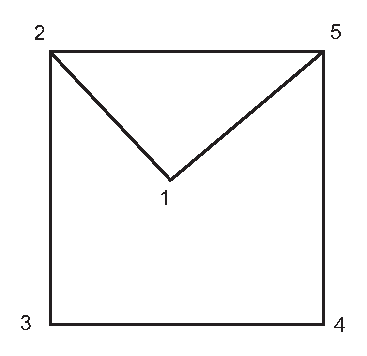
\includegraphics{PS/no4circuit.eps}
  \caption{A $4$-circuit}
  \label{fig:no4circuit}
\end{figure}

Suppose that $D$ is a decomposition star whose associate graph
contains such triangular and pentagonal standard regions.  Recall
that $D$ determines a set $U(D)$ of vertices in Euclidean $3$-space
of distance at most $2t_0$ from the origin, and that each vertex
$p_i$ can be realized geometrically as a point on the unit sphere at
the origin, obtained as the radial projection of some $v_i\in U(D)$.

\begin{lemma}  One of the edges $\{v_1,v_3\}$, $\{v_1,v_4\}$ has
length less than $2\sqrt{2}$.  Both of the them have lengths less
than $3.02$. Also, $|v_1|\ge2.3$.
\end{lemma}

\begin{proof}
This is a standard exercise in geometric considerations as
introduced in Section~\ref{sec:decomposition}.  (The reader should
review that section for the framework of the following argument.)
We deform the figure using pivots to a configuration
$v_2,\ldots,v_5$ at height $2$, and $|v_i-v_j|=2t_0 $,
$(i,j)=(2,3),(3,4),(4,5),(5,2)$. We scale $v_1$ until $|v_1|=2t_0
$. We can also take the distance from $v_1$ to $v_5$ and to $v_2$
to be $2$. If we have $|v_1-v_3|\ge 2\sqrt{2}$, then we stretch
the edge $|v_1-v_4|$ until $|v_1-v_3|=2\sqrt{2}$. The resulting
configuration is rigid.  Pick coordinates to find that
$|v_1-v_4|<2\sqrt{2}$. If we have $|v_1-v_3|\ge 2t_0 $, follow a
similar procedure to reduce to the rigid configuration
$|v_1-v_3|=2t_0$, to find that $|v_1-v_4|<3.02$. The estimate
$|v_1|\ge2.3$ is similar.
\end{proof}

There are restrictive bounds on the dihedral angles of the
simplices $\{0,v_1,v_i,v_j\}$ along the edge $\{0,v_1\}$. The
quasi-regular tetrahedron has a dihedral angle of at most%
\footnote{\calc{984463800}} $1.875$.  The dihedral angles of the
simplices $\{0,v_1,v_2,v_3\}$, $\{0,v_1,v_5,v_4\}$
adjacent to it are at most%
\footnote{\calc{821707685}}  $1.63$. The dihedral angle of the
remaining simplex $\{0,v_1,v_3,v_4\}$ is at most%
\footnote{\calc{115383627}} $1.51$.   This leads to lower bounds
as well. The quasi-regular tetrahedron has a dihedral angle that
is at least $2\pi - 2(1.63)-1.51 > 1.51$.  The dihedral angles
adjacent to the quasi-regular tetrahedron is at least $2\pi-
1.63-1.51-1.875> 1.26$. The remaining dihedral angle is at least
$2\pi-1.875-2(1.63) > 1.14$.

A decomposition star $D$ determines a set of vertices $U(D)$ that
are of distance at most $2t_0$ from the center of $D$.  Three
consecutive vertices $p_1$, $p_2$, and $p_3$ of a standard region
are determined as the projections to the unit sphere of three
corners $v_1$, $v_2$, and $v_3$, respectively in $U(D)$. By
Lemma~\ref{lemma:1.32}, if the interior angle of the standard
region is less than $1.32$, then $|v_1-v_3|\le\sqrt{8}$.

\begin{lemma} \label{lemma:11.16}
These two standard regions $F=\{R_1,R_2\}$ give
    $\tau_F(D) \ge 11.16\,\pt$.
\end{lemma}

\begin{proof}
Let $\dih$ denote the dihedral angle of a simplex along a given
edge. Let $S_{ij}$ be the simplex $\{0,v_1,v_i,v_j\}$, for
$(i,j)=(2,3),(3,4), (4,5),(2,5)$. We have $\sum_{(4)}\dih(S_{ij})
= 2\pi$. Suppose one of the edges $\{v_1,v_3\}$ or $\{v_1,v_4\}$ has
length $\ge2\sqrt2$. Say $\{v_1,v_3\}$.

We have\footnote{\calc{572068135}, \calc{723700608},
\calc{560470084}, and \calc{535502975}}
    $$
    \begin{array}{lll}
    \tau(S_{25}) &- 0.2529\dih(S_{25}) > -0.3442,\\
    \tau_0(S_{23}) &- 0.2529\dih(S_{23}) > -0.1787,\\
    \hat\tau(S_{45}) &- 0.2529\dih(S_{45}) > -0.2137,\\
    \tau_0(S_{34}) &- 0.2529\dih(S_{34}) > -0.1371.\\
    \end{array}
    $$
We have a penalty $\xiG$ for erasing, so that
    $$
    \begin{array}{lll}
        \tau(D) &\ge \sum_{(4)}\tau_x(S_{ij}) - 5\xiG\\
                &>2\pi(0.2529)-0.3442\\
                &\qquad -0.1787-0.2137-0.1371-5\xiG\\
                &>11.16\,\pt,
    \end{array}
    $$
where $\tau_x=\tau,\hat\tau,\tau_0$ as appropriate.

Now suppose $\{v_1,v_3\}$ and $\{v_1,v_4\}$ have length $\le2\sqrt2$.
If there is an upright diagonal that is not enclosed over either
flat quarter, the penalty is at most $3\xiG+2\xiV$. Otherwise, the
penalty is smaller: $4\xiG'+\xiV$. We have
    $$
    \begin{array}{lll}
    \tau(D)
    &\ge \sum_{(4)}\tau(S_{ij})-(3\xiG+2\xiV)\\
    &>2\pi(0.2529)-0.3442\\
    &\qquad -2(0.2137)-0.1371 -(3\xiG+2\xiV)\\
    &>11.16\,\pt.\\
    \end{array}
    $$
\end{proof}

\section{A particular $5$-circuit}

\begin{lemma}\label{lemma:6079}  Assume that $R$ is a pentagonal standard region
    with an enclosed vertex $v$ of height at most $2t_0$.
    %(See Figure~\ref{fig:pent-tri1}.)
    Assume further that
    \begin{itemize}
        \item $|v_i|\le 2.168$ for each of the five corners.
        \item Each interior angle of the pentagon is at most
        $2.89$.
        \item If $v_1$, $v_2$, $v_3$ are consecutive corners over
        the pentagonal region, then $$|v_1-v_2|+|v_2-v_3|<4.804.$$
        \item $\sum_5 |v_i-v_{i+1}|\le 11.407.$
    \end{itemize}
    Then $\sigma_R(D)< -0.2345$ or $\tau_R(D) > 0.6079.$
\end{lemma}

%\begin{figure}[htb]
%  \centering
%  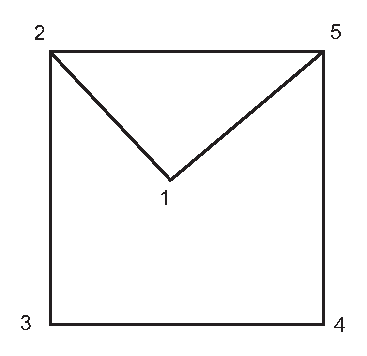
\includegraphics{PS/no4circuit.eps}
%  \caption{A pentagon and triangle}
%  \label{fig:pent-tri1}
%\end{figure}


\begin{proof}
Since $-0.4339$ is less than this the lower bound, a $3$-crowded
upright diagonal does not occur. Similarly, since $-0.25$ is less
than the lower bound, a $4$-crowded upright diagonal does not
occur (Lemma~\ref{lemma:4-crowded} and Lemma~\ref{x-3.8}).

Suppose that there is a loop in context $(n,k)=(4,2)$. Again by
Lemma~\ref{lemma:loop} (with $n(R)=7$),
$$\sigma_R(D)  < -0.2345.$$
%The constants come from
%Table~\ref{x-5.11} and  Theorem~\ref{thm:the-main-theorem}.

%If we branch and bound on the triangular faces, this LP-derived
%inequality can be improved to
%    $$\tau[F] < 0.6079.$$

%If there is a loop other than $(4,2)$ and $(4,1)$, the linear
%program becomes infeasible:
%    $$\tau[F] < 0.644 < t_7 + \dloop(n,k) < \tau[F].$$
We conclude that all loops have context $(n,k)=(4,1)$.


{\bf Case 1.}  {\it The vertex $v=v_{12}$ has distance at least
$2t_0$ from the five corners of $U(D)$ over the pentagon.}

%The interval calculations relevant in Case 1 appear in
%~\ref{A.3.8}.

The penalty to switch the pentagon to a pure $\vor_0$ score is at
most $5\xiG$ (see Section~\ref{sec:prep-cluster}).  There cannot
be two flat quarters because then
$$|v_{12}|>\CalE(S(2,2,2,2t_0,2\sqrt2,2\sqrt2),2t_0,2t_0,2t_0)>2t_0.$$

{\bf (Case 1-a)} Suppose there is one flat quarter,
$|v_1-v_4|\le2\sqrt2$. There is a lower bound of 1.2 on the
dihedral angles of the simplices $\{0,v_{12},v_i,v_{i+1}\}$.  This
is obtained as follows.  The proof relies on the convexity of the
quadrilateral region.  We leave it to the reader to verify that
the following pivots can be made to preserve convexity.  Disregard
all vertices except $v_1,v_2,v_3,v_4,v_{12}$.  We give the
argument that $\dih(0,v_{12},v_1,v_4)>1.2$.  The others are
similar. Disregard the length $|v_1-v_4|$.  We show that
    $$
    \begin{array}{lll}
        sd &:=\dih(0,v_{12},v_1,v_2)+\dih(0,v_{12},v_2,v_3)\\
           &+\dih(0,v_{12},v_3,v_4) < 2\pi-1.2.
    \end{array}
    $$
Lift $v_{12}$ so $|v_{12}|=2t_0$. Maximize $sd$ by taking
$|v_1-v_2|=|v_2-v_3|=|v_3-v_4|=2t_0$.  Fixing $v_3$ and $v_4$,
pivot $v_1$ around $\{0,v_{12}\}$ toward $v_4$, dragging $v_2$
toward $v_{12}$ until $|v_2-v_{12}|=2t_0$.  Similarly, we obtain
$|v_3-v_{12}|=2t_0$. We now have $sd\le 3(1.63)< 2\pi-1.2$, by a
calculation.\footnote{\calc{821707685}}

Return to the original figure and move $v_{12}$ without increasing
$|v_{12}|$ until each simplex $\{0,v_{12},v_i,v_{i+1}\}$ has an edge
$(v_{12},v_j)$ of length $2t_0$. Interval
calculations\footnote{\calc{467530297} and \calc{135427691}} show
that the four simplices around $v_{12}$ squander
    $$2\pi(0.2529)-3(0.1376)-0.12 > \squander + 5\xiG.$$

{\bf (Case 1-b)} Assume there are no flat quarters. By hypothesis,
the perimeter satisfies $$\sum|v_i-v_{i+1}|\le 11.407.$$ We have
$\arc(2,2,x)'' = 2x/(16-x^2)^{3/2} >0$. The arclength of the
perimeter is therefore at most
$$2\arc(2,2,2t_0) + 2\arc(2,2,2) + \arc(2,2,2.387) <  2\pi.$$
There is a well-defined interior of the spherical pentagon, a
component of area $<2\pi$.  If we deform by decreasing the
perimeter, the component of area $<2\pi$ does not get swapped with
the other component.

Disregard all vertices but $v_1,\ldots,v_5,v_{12}$.  If a vertex
$v_i$ satisfies  $|v_i-v_{12}|>2t_0$, deform $v_i$ as in
Section~\ref{x-4.9} until $|v_{i-1}-v_{i}|=|v_i-v_{i+1}|=2$, or
$|v_i-v_{12}|=2t_0$. If at any time, four of the edges realize the
bound $|v_i-v_{i+1}|=2$, we have reached an impossible situation,
because it leads to the contradiction\footnote{\calc{115383627}
and \calc{603145528}}
    $$2\pi = \sum^{(5)}\dih < 1.51 + 4 (1.16) < 2\pi.$$
(This inequality relies on the observation, which we leave to the
reader, that in any such assembly, pivots can by applied to bring
$|v_{12}-v_i|=2t_0$ for at least one edge of each of the five
simplices.)



The vertex $v_{12}$ may be moved without increasing $|v_{12}|$ so
that eventually by these deformations (and reindexing if
necessary) we have $|v_{12}-v_i|=2t_0$, $i=1,3,4$. (If we have
$i=1,2,3$, the two dihedral angles along $\{0,v_2\}$
satisfy\footnote{\calc{115383627}} $<2(1.51)<\pi$, so the
deformations can continue.)



There are two cases. In both cases $|v_i-v_{12}|=2t_0$, for
$i=1,3,4$.
$$
\begin{array}{lll}
(i)\quad &|v_{12}-v_2|=|v_{12}-v_5|=2t_0,\\
(ii)\quad &|v_{12}-v_2|=2t_0,\quad |v_4-v_5|=|v_5-v_1|=2,\\
\end{array}
$$
Case (i) follows from interval
calculations\footnote{\calc{312132053}}
$$
\sum\tau_0 \ge 2\pi(0.2529) - 5 (0.1453) > 0.644+7\xiG.
$$
In case (ii), we have again
    $$2\pi(0.2529)-5 (0.1453).$$
In this interval calculation we have assumed that
$|v_{12}-v_5|<3.488$. Otherwise, setting $S=(v_{12},v_4,v_5,v_1)$,
we have
    $$\Delta(S) < \Delta(3.488^2,4,4,8,(2t_0)^2,(2t_0)^2)<0,$$
and the simplex does not exist.  ($|v_4-v_1|\ge2\sqrt2$ because
there are no flat quarters.) This completes Case 1.

\medskip

{\bf Case 2.} {\it The vertex $v_{12}$ has distance at most $2t_0$
from the vertex $v_1$ and distance at least $2t_0$ from the
others.}

Let $\{0,v_{13}\}$ be the upright diagonal of a loop $(4,1)$.  The
vertices of the loop are not $\{v_2,v_3,v_4,v_5\}$ with $v_{12}$
enclosed over $\{0,v_2,v_5,v_{13}\}$ by
Lemma~\ref{lemma:anc-simplex-not-enc}. The vertices of the loop
are not $\{v_2,v_3,v_4,v_5\}$ with $v_{12}$ enclosed over
$\{0,v_1,v_2,v_5\}$ because this would lead to a contradiction
$$y_{12}\ge \CalE(S(2,2,2,2t_0,2t_0,3.2),2t_0,2t_0,2)>2t_0,$$
or
$$y_{12}\ge \CalE(S(2,2,2,2t_0,2t_0,3.2),2,2t_0,2)>2t_0.$$
We get a contradiction for the same reasons
 unless $\{v_1,v_{12}\}$ is an edge of some
upright quarter of every loop of type $(4,1)$.

We consider two cases.  (2-a) There is a flat quarter along an
edge other than $\{v_1,v_{12}\}$.  That is, the central vertex is
$v_2$, $v_3$, $v_4$, or $v_5$.  (Recall that the {\it central
vertex} of a flat quarter is the vertex other than the origin that
is not an endpoint of the diagonal.) (2-b) Every flat quarter has
central vertex $v_1$.

{\bf Case 2-a.}  We erase all upright quarters including those in
loops, taking penalties as required. There cannot be two flat
quarters by geometric considerations
$$
\begin{array}{lll}
\CalE(S(2,2,2,2\sqrt2,2\sqrt2,2t_0),2t_0,2t_0,2)&>2t_0\\
\CalE(S(2,2,2,2\sqrt2,2\sqrt2,2t_0),2,2t_0,2t_0)&>2t_0\\
\end{array}
$$

The penalty is at most $7\xiG$.  We show that the region (with
upright quarters erased) squanders $>7\xiG+0.644$.  We assume that
the central vertex is $v_2$ (case 2-a-i) or $v_3$ (case 2-a-ii).
In case 2-a-i, we have three types of simplices around $v_{12}$,
characterized by the bounds on their edge lengths.  Let
$\{0,v_{12},v_1,v_5\}$ have type A, $\{0,v_{12},v_5,v_4\}$ and
$\{0,v_{12},v_4,v_3\}$ have type B, and let $\{0,v_{12},v_3,v_1\}$
have type C.  In case 2-a-ii there are also three types.  Let
$\{0,v_{12},v_1,v_2\}$ and $\{0,v_{12},v_1,v_5\}$ have type A,
$\{0,v_{12},v_5,v_4\}$ type B, and $\{0,v_{12},v_2,v_4\}$ type D.
(There is no relation here between these types and the types of
simplices $A$, $B$, $C$ defined in \Chap~\ref{sec:fine}.) Upper
bounds on the dihedral angles along the edge $\{0,v_{12}\}$ are
given as calculations\footnote{\calc{821707685}, \calc{115383627},
\calc{576221766}, and \calc{122081309}}. These upper bounds come
as a result of a pivot argument similar to that establishing the
bound 1.2 in Case 1-a.

These upper bounds imply the following lower bounds.  In case
2-a-i,
$$
\begin{array}{lll}
\dih &> 1.33 \quad(A),\\
\dih &> 1.21 \quad(B),\\
\dih &> 1.63 \quad(C),\\
\end{array}
$$
and in case 2-a-ii,
$$
\begin{array}{lll}
\dih &> 1.37 \quad(A),\\
\dih &> 1.25 \quad(B),\\
\dih &> 1.51 \quad(D),\\
\end{array}
$$
In every case the dihedral angle is at least $1.21$. In case
2-a-i, the inequalities give a lower bound on what is squandered
by the four simplices around $\{0,v_{12}\}$. Again, we move $v_{12}$
without decreasing the score until each simplex
$\{0,v_{12},v_i,v_{i+1}\}$ has an edge satisfying
$|v_{12}-v_j|\le2t_0$. Interval
calculations\footnote{\calc{644534985}, \calc{467530297}, and
\calc{603910880}} give
    $$
    \begin{array}{lll}
    \sum_{(4)}\tau_0 &> 2\pi (0.2529) - 0.2391-2(0.1376)-0.266\\
        &>0.808.
    \end{array}
    $$
In case 2-a-ii, we have\footnote{\calc{135427691}}
    $$
    \begin{array}{lll}
    \sum_{(4)}\tau_0 &> 2\pi (0.2529) - 2(0.2391)-0.1376-0.12\\
        &>0.853.
    \end{array}
    $$
So we squander more than $7\xiG+0.644$, as claimed.

{\bf Case 2-b.}  We now assume that there are no flat quarters
with central vertex $v_2,\ldots,v_5$. We claim
 that $v_{12}$ is not enclosed over $\{0,v_1,v_2,v_3\}$ or
$\{0,v_1,v_5,v_4\}$. In fact, if $v_{12}$ is enclosed over
$\{0,v_1,v_2,v_3\}$, then we reach the
contradiction\footnote{\calc{821707685} and \calc{115383627}}
    $$
    \begin{array}{lll}
    \pi&<\dih(0,v_{12},v_1,v_2)+\dih(0,v_{12},v_2,v_3)\\
        &< 1.63+1.51 < \pi.
    \end{array}
    $$

We claim
 that $v_{12}$ is not enclosed over $\{0,v_5,v_1,v_2\}$.
Let $S_1=\{0,v_{12},v_1,v_2\}$, and $S_2=\{0,v_{12},v_1,v_5\}$.  We
have by hypothesis,
$$y_4(S_1)+y_4(S_2) = |v_1-v_2|+|v_1-v_5|< 4.804.$$
An interval calculation\footnote{\calc{69064028}} gives
    $$
    \begin{array}{lll}
    \sum_{(2)}\dih(S_i) &\le \sum_{(2)}
    \left(\dih(S_i)+0.5(0.4804/2-y_4(S_i))\right)\\
    &<\pi.
    \end{array}
    $$
So $v_{12}$ is not enclosed over $\{0,v_1,v_2,v_5\}$.

Erase all upright quarters, taking penalties as required.  Replace
all flat quarters with $\svor_0$-scoring taking penalties as
required. (Any flat quarter has $v_1$ as its central vertex.) We
move $v_{12}$ keeping $|v_{12}|$ fixed and not decreasing
$|v_{12}-v_1|$.  The only effect this has on the score comes
through the quoins along $\{0,v_1,v_{12}\}$. Stretching
$|v_{12}-v_1|$ shrinks the quoins and increases the score. (The
sign of the derivative of the quoin with respect to the top edge
is computed in the proof of Lemma~\ref{x-4.9.1}.)

If we stretch $|v_{12}-v_1|$ to length $2t_0$, we are done by case
1 and case 2-a. (If deformations produce a flat quarter, use case
2-a, otherwise use case 1.) By the claims, we can eventually
arrange (reindexing if necessary) so that
$$
\begin{array}{lll}
(i)&\quad |v_{12}-v_3|=|v_{12}-v_4|=2t_0,\quad\text{or}\\
(ii)&\quad |v_{12}-v_3|=|v_{12}-v_5|=2t_0.
\end{array}
$$
We combine this with the deformations of Section~\ref{x-4.9} so
that in case (i) we may also assume that if $|v_5-v_{12}|>2t_0$,
then $|v_4-v_5|=|v_5-v_1|=2$ and that if $|v_2-v_{12}|>2t_0$, then
$|v_1-v_2|=|v_2-v_3|=2$. In case (ii) we may also assume that if
$|v_4-v_{12}|>2t_0$, then $|v_3-v_4|=|v_4-v_5|=2$ and that if
$|v_2-v_{12}|>2t_0$, then $|v_1-v_2|=|v_2-v_3|=2$.

Break the pentagon into subregions by cutting along the edges
$(v_{12},v_i)$ that satisfy $|v_{12}-v_i|\le2t_0$. So for example
in case (i), we cut along $(v_{12},v_3)$, $(v_{12},v_4)$,
$(v_{12},v_1)$, and possibly along $(v_{12},v_2)$ and
$(v_{12},v_5)$.  This breaks the pentagon into triangular and
quadrilateral regions.

In case (ii), if $|v_4-v_{12}|>2t_0$, then the argument used in
Case 1 to show that $|v_4-v_{12}|<3.488$ applies here as well. In
case (i) or (ii), if $|v_{12}-v_2|>2t_0$, then for similar
reasons, we may assume
    $$\Delta(|v_{12}-v_2|^2,4,4,8,(2t_0)^2,|v_{12}-v_1|^2)\ge0.$$
This justifies the hypotheses for the
calculations\footnote{\calc{312132053} and \calc{644534985}} that
we use. We conclude that
    $$\sum\tau_0 \ge 2\pi (0.2529) -3 (0.1453) -2 (0.2391) > 0.6749.$$
If the penalty is less than $0.067=0.6749-0.6079$, we are done.

We have ruled out the existence of all loops except $(4,1)$. Note
that a flat quarter with central vertex $v_1$ gives penalty at
most $0.02$ by Lemma~\ref{x-3.11.3}.
  If there is at most one
such a flat quarter and at most one loop, we are done:
$$3\xiG + 0.02 < 0.067.$$
Assume there are two loops of context $(n,k)=(4,1)$.  They both
lie along the edge $\{v_1,v_{12}\}$, which precludes any unmasked
flat quarters. If one of the upright diagonals has height
$\ge2.696$, then the penalty is at most $3\xiG+3\xiV< 0.067$.
Assume both heights are at most $2.696$. The total interior angle
of the exceptional face at $v_1$ is at least four times the
dihedral angle of one of the flat quarters along $\{0,v_1\}$, or
$4(0.74)$ by an interval calculation\footnote{\calc{751442360}}. This is
contrary to the hypothesis of an interior angle $<2.89$.   This
completes Case 2. This shows that heptagons with pentagonal hulls
do not occur.
\end{proof}

\begin{lemma}\label{lemma:excess-1}
Let $R$ be an exceptional standard region.  Let $V$
be a set of vertices of $R$.  If $v\in V$, let $p_v$ be the number
of triangular regions at $v$ and let $q_v$ be the number of
quadrilateral regions at $v$.  Assume that $V$ has the following
properties:
    \begin{enumerate}
        \item No two
        vertices in $V$ are adjacent.
        \item No two vertices
        in $V$ lie on a common quadrilateral.
        \item If $v\in V$, then there are five standard regions at
        $v$.
        \item If $v\in V$, then the corner over $v$ is a central
        vertex of a flat quarter in the cone over $R$.
        \item If $v\in V$, then $p_v\ge 3$.  That is, at least
        three of the five standard regions at $v$ are triangular.
        \item If $R'\ne R$ is an exceptional region at $v$, and if $R$
        has interior angle at least $1.32$ at $v$, then $R'$ also has interior
        angle at least $1.32$ at $v$.
        \item If $(p_v,q_v)=(3,1)$, then the internal angle at $v$ of the exceptional
        region is at most $1.32$.
    \end{enumerate}
  Define $a:\N\to \R$ by
  $$a(n) = \begin{cases}
    14.8 &n=0,1,2,\\
    1.4 & n=3,\\
    1.5 & n=4,\\
    0 & \text{otherwise.}
  \end{cases}
  \index{aZ@$a(n)$}
  $$
Let $\{F\}$ be the union of $\{R\}$ with the set of triangular and
quadrilateral regions that have a vertex at some $v\in V$. Then
    $$\sum_F\tau_F(D) > \sum_{v\in V} (p_v d(3) + q_v d(4) + a
    (p_v))\,\pt.$$
\end{lemma}

\begin{proof}   We erase all upright diagonals in the
$Q$-system, except for those that carry a penalty: loops,
$3$-unconfined, $3$-crowded, and $4$-crowded diagonals.

We assume that if $(p_v,q_v)=(3,1)$, then the internal angle is at
most $1.32$. Because of this, if we score the flat quarter by
$\vor_0$, then the flat quarter $Q$ satisfies
(Lemma~\ref{lemma:1.32})
   \begin{equation}
   \vor_0(Q) > 3.07\,\pt > 1.4\,\pt + D(3,1) + 2\xiV + \xiG.
   \label{eqn:307}
   \end{equation}



Every flat quarter that is masked by a remaining upright quarter
in the $Q$-system has $y_4\ge2.6$.  Moreover, $y_1\ge2.2$ or
$y_4\ge2.7$.  Let $\pi_v = 2\xiV + \xiG$ if the flat quarter is
masked, and $\pi_v = 0$ otherwise.

We claim that the flat quarter (scored by $\vor_0$) together with
the triangles and quadrilaterals at a given vertex $v$ squander at
least
   \begin{equation}
   (p_v d(3) + q_v d(4) + a(p_v))\,\pt + D(3,1) + \pi_v
   \label{eqn:one-v}
   \end{equation}
If $p_v=4$, this is \calc{314974315}.  If $p_v=3$, we may assume
by the preceding remarks that there are two exceptional regions at
$v$.  If the internal angle of $R$ at $v$ is at most $1.32$, then
we use Inequality~\ref{eqn:307}.  If the angle is at least $1.32$,
then by hypothesis, the angle $R'$ at $v$ is at least $1.32$.  We
then appeal to the calculations \calc{675785884} and
\calc{193592217}.

To complete the proof of the lemma, it is enough to show that we
can erase the upright quarters masking a flat quarter at $v$
without incurring a penalty greater than $\pi_v$.  For then, by
summing the Inequality~\ref{eqn:one-v} over $v$, we obtain the
result.

If the upright diagonal is enclosed over the masked flat quarter,
then the upright quarters can be erased with penalty at most
$\xiV$ (by Remark~\ref{remark:3rd-quarter}). Assume the upright
diagonal is not enclosed over the masked flat quarter.

If there are at most three upright quarters, the penalty is at
most $2\xiV + \xiG$.  Assume four or more upright quarters.  If
the upright diagonal is not a loop, then it must be $4$-crowded.
This can be erased with penalty
   $$2\xiV + 2\xiG - \kappa < 2\xiV + \xiG.$$

Finally, assume that the upright quarter is a loop with four or
more upright quarters.  Lemma~\ref{lemma:loop} limits the
possibilities to parameters $(5,0)$ or $(5,1)$.  In the case of a
loop $(5,1)$, there is no need to erase because $|V|\le3$ and by
Lemma~\ref{lemma:loop}, the hexagonal standard region squanders at
least
   $$t_6 + 3 a(p_v)\,\pt$$
as required by the lemma.  In the case of a loop $(5,0)$ in a
pentagonal region, if $|V|=1$ then there is no need to erase
(again we appeal to Lemma~\ref{lemma:loop}).  If $|V| =2$, then
the two vertices share a penalty of $4\xiV + \xiG$, with each
receiving
   $$2\xiV + \xiG/2 < 2\xiV +\xiG.$$
\end{proof}

    }

%%%%%%%%%%%%%%%%%%%%%%%%%%%%%%%%%%%%%%%%%%%%%%%%%%%%
%%%%%%%%%%%%%%%%%%%%%%%%%%%%%%%%%%%%%%%%%%%%%%%%%%%%

\longversion{
    \part{Sphere Packings V. Pentahedral Prisms -- Ferguson}
    \label{part:ferguson}
    \chapter*{Introduction}
    %% SPV Intro

This paper is the fifth in a series of papers devoted to the proof
of the Kepler conjecture, which asserts that no packing of congruent
balls in three dimensions has density greater than the face-centered
cubic packing.

In this paper, we prove that decomposition stars associated with the
plane graph of arrangements we term pentahedral prisms do not
contravene.  Recall that a contravening decomposition star is a
potential counterexample to the Kepler conjecture. We use interval
arithmetic methods to prove particular linear relations on
components of any such contravening decomposition star.  These
relations are then combined to prove that no such contravening stars
exist.

Pentahedral prisms come remarkably close to achieving the optimal
score of $8 \myscorept$, that achieved by the decomposition stars of
the face-centered cubic lattice packing. In this sense, we consider
pentahedral prisms to be ``worst case" decomposition stars.

Pentahedral prisms constituted a counterexample to an early version
of Hales's approach to a proof of the Kepler conjecture, and have
always been a somewhat thorny obstacle to the proof of the
conjecture. Relations required to treat pentahedral prisms are
delicate in contrast to the more general bounds which suffice  to
treat other decomposition stars.

This paper is a revised version of the author's PhD thesis at the
University of Michigan.  The author wishes to thank Tom Hales, Jeff
Lagarias and the referees for their many contributions to this
revision.

    %% Changes in Ferguson's part needed to merge it with other papers:
%% cite{sp1} --> cite{part1}.
%% includegraphics{ --> includegraphics{ferguson2005B/       }}
%% begin{calc} --> begin{calcf}
%% end{calc} --> end{calcf}
%% His hard cross references need to be made soft.

%Draft of Samuel Ferguson's Thesis, Spring 1997.

\chapter{Pentahedral Prisms}
Recall that a {\em contravening
decomposition star} is a potential counterexample to the
Kepler conjecture.  The subject of this paper is a particular class of potentially contravening
decomposition stars.

We use the term {\em pentahedral prisms} to refer to this class of potentially
contravening decomposition stars, and refer to a decomposition star in this
class as a {\em pentahedral prism}.  This class is defined by the plane graph in
Figure~\ref{fig:pentagraph}.

\begin{figure}
\begin{center}
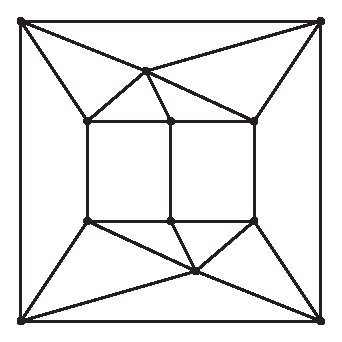
\includegraphics{PS/pentagraph}
\end{center}
%\includegraphics{pentaface}
%\centerline{ \psfig{file=pentaface.eps} }
\caption{The plane graph of a pentahedral prism.}
\label{fig:pentagraph}
\end{figure}

An example of an arrangement with such a graph is depicted in Figure~\ref{fig:penta2}.

\begin{figure}
\begin{center}
\includegraphics{PS/pentaballs}
\end{center}
%\centerline{ \psfig{file=pentaballs.eps} }
\caption{Spheres in a pentahedral prism arrangement.}
\label{fig:penta2}
\end{figure}

A pentahedral prism is characterized by the arrangement and
combinatorics of its standard regions.  It is composed of ten triangular
standard regions, and five quadrilateral standard regions.

The ten triangles are arranged in two
{\em pentahedral caps}, five triangles arranged around a common vertex.
The five quadrilaterals lie in a band between the two caps.
See Figure~\ref{fig:pentaface}.

\begin{figure}
\begin{center}
\includegraphics{PS/pentaface}
\end{center}
%\centerline{ \psfig{file=pentaface.eps} }
\caption{The faces of a pentahedral prism.}
\label{fig:pentaface}
\end{figure}

Recall that the standard cluster attached to a triangular standard region
is a \qrtet.  Likewise, the standard cluster attached to a
quadrilateral is a quad cluster.
We use the term pentahedral cap to refer to
both the standard regions and the \qrtets\ which comprise it.

%\begin{remark}
%In the earliest formulation,  pentahedral prisms
%could score more than $8 \myscorept$.  Pentahedral prisms appeared, on an experimental
%basis, to be the only counterexamples to the potential success of
%the Hales program.  To a certain degree, the pursuit of a proof  that such stars score less than
%$8 \myscorept$ drove the evolution of both the decomposition of space and the
%scoring function.

%Pentahedral prisms still come remarkably
%close to achieving the optimal score of $8 \myscorept$, that achieved by the
%decomposition stars of the face-centered cubic lattice packing.
%In this sense, we consider pentahedral prisms
%to be ``worst case" decomposition stars.

%Thus far,
%the relations required to treat pentahedral prisms have been
%delicate in contrast to the more general bounds which have to date
%sufficed to treat other decomposition stars.

%\end{remark}


\section{The Main Theorem}
\label{sec:dabound} We begin by recalling various definitions from
Paper II, Formulation.  The constant $\myscorept$ is introduced in
Definition~\ref{def:pt}\tomcite.  Similarly, {\em score} is defined
in Theorem~\ref{lemma:negligible'}\tomcite, as well as
Definition~\ref{def:sigma}\tomcite\ and
Remark~\ref{remark:vor}\tomcite. We denote the score of a region $R$
by $\myscore(R)$.

\begin{thm}
\label{thm:dabound}
Each pentahedral prism $P$ satisfies
\[\myscore(P) \le (8 - \epsilon_0) \myscorept\]
for $\epsilon_0 = 10^{-8}$.  Hence there are no contravening pentahedral prisms.
\end{thm}

The next section will introduce a series of propositions which will prove the main theorem.
The first proposition will restrict our attention to a set of potentially contravening pentahedral prisms.
Subsequent propositions  will provide a collection of relations which we will use to prove the main theorem.

\section{Propositions}
\label{sec:props} The function $sol(\cdot)$ is introduced in
Definition~\ref{def:sol}\tomcite.  The function $dih(\cdot)$ is
introduced in Definition~\ref{def:dih}\tomcite.

We present computations using auxiliary bounds
which imply the main result of the paper, that the
score of any pentahedral prism is strictly less than $8 \myscorept$.

Recall from Section~\ref{sec:ssc}\tomcite\ that the score
decomposition for a decomposition star $S$ takes the form
\[\myscore(S) = \sum_R\myscore(R)\]
where $R$ runs over the standard clusters in $S$.

In the case of a pentahedral prism $P$, the score $\myscore(P)$ decomposes
as
\[\myscore(P) = \sum_{i=1}^{10}\myscore(T_i) + \sum_{j=1}^5\myscore(Q_j)\]
with the triangular regions $T_i$ numbered so that the two pentahedral
caps $C_i$ consist of $\{T_i: 1 \le i \le 5\}, \{T_i : 6 \le i \le 10\}$ and $Q_j$ denote
the quad clusters.  Thus
\[ \myscore(C_1) = \sum_{i=1}^5 \myscore(T_i), \text{ \ \ \ } \myscore(C_2) = \sum_{i=6}^{10} \myscore(T_i).\]

% The argument for the nonexistence of a contravening configuration is by contradiction.
% We assume there exists a pentahedral prism with score at least $8 \myscorept$ and derive inequalities % showing that its score is strictly less than $8 \myscorept$.  This proves no such decomposition star exists.

The following proposition gives basic inequalities which we will use to form a restricted set of
pentahedral prisms.

%We use the following lemma to restrict our attention to potentially contravening pentahedral
%prisms.

\begin{prop}
\label{prop:pentscorebd}
A pentahedral prism $P$ satisfies the bound
\[\myscore(P) \le (8 - \epsilon_0) \myscorept\]
for $\epsilon_0 = 10^{-8}$ provided that any one of the following conditions holds:
\begin{enumerate}
\item $P$ contains a tetrahedron $T$ such that
    \[\myscore(T) \le -0.52 \myscorept\] \label{eq:triangle}
\item $P$ contains a quad cluster $Q$ such that
    \[\myscore(Q) \le -1.04 \myscorept\] \label{eq:quad}
\item $P$ contains a pentahedral cap $C$ such that
    \[\myscore(C) \le 3.48 \myscorept\]  \label{eq:penta}
\end{enumerate}
\end{prop}

%\begin{  enumerate}
%item Triangular regions score $ -0.52 \myscorept$
%\item Quad clusters score $> -1.04 \myscorept$
%\item Pentahedral caps score $> 3.48 \myscorept$
%\end{enumerate}
%\begin{eqnarray}
% \myscore(T) & > & -0.52 \myscorept   \label{eq:triangle}   \\
% \myscore(Q) & > & -1.04 \myscorept  \label{eq:quad}        \\
% \myscore(C) & > & 3.48 \myscorept   \label{eq:penta}
%\end{eqnarray}

\begin{proof}
We use the following scoring bounds proved earlier for any admissible decomposition star.

First, Lemma~\ref{lemma:1pt}\tomcite\ states that any \qrtet\ $T$
satisfies
    \[\myscore(T) \le 1 \myscorept. \]

Theorem~\ref{lemma:quad0}\tomcite\ states that any quad cluster $Q$
satisfies
    \[\myscore(Q) \le 0.\]

Next, a pentahedral cap $C$ consists of five quasi-regular
tetrahedra $T_i$ sharing a common distinguished edge.  At one end of
the distinguished edge is the distinguished vertex $v=0$ which is
the center of the decomposition star $P$.  Each $T_i$ has context
$c_i = (5, 0)$. Lemma~\ref{lemma:0.55}\tomcite\ (with $k=1$ and
$r=5$) and Lemma~\ref{lemma:0.55A}\tomcite\ state that any
pentahedral cap $C_i$ satisfies
    \[\myscore(C_i) = \sum_{i=1}^5 \myscore(T_i,c_i,v) \le (4.52 - \epsilon_0) \myscorept\]
with $\epsilon_0 = 10^{-8}$.

\begin{enumerate}
\item Suppose that some $\myscore(T) \le -0.52 \myscorept$, with $T$ contained in a pentahedral cap $C_1$.
Then the inequalities above give
\begin{eqnarray*}
\myscore & \le & -0.52 \myscorept + 4(1 \myscorept) + \myscore(C_2) + \sum_{j=1}^5\myscore(Q_j)    \\
                 & \le & 3.48 \myscorept  + (4.52 - \epsilon_0) \myscorept + 5(0) = (8 - \epsilon_0) \myscorept
\end{eqnarray*}

\item Suppose that some quad cluster $\myscore(Q_j) \le -1.04 \myscorept$.  Then
\begin{eqnarray*}
\myscore(P) & \le & \myscore(C_1) + \myscore(C_2) + (-1.04 \myscorept) + 4(0)    \\
                 & \le & 2((4.52 - \epsilon_0) \myscorept) -(1.04 \myscorept) = (8 - 2\epsilon_0) \myscorept
\end{eqnarray*}
\item Suppose that some pentahedral cap $C_1$ has $\myscore(C_1) \le 3.48 \myscorept$.
Then the inequalities above give
    \[\myscore(P) \le (3.48 \myscorept) + (4.52 - \epsilon_0) \myscorept + 5(0) = (8 - \epsilon_0) \myscorept\]
\end{enumerate}

This completes the proof.
\end{proof}

%\begin{cor}
%\label{cor:pentscorebd}
%The score of any  pentahedral prism excluded by
%Proposition~\ref{prop:pentscorebd} is bounded above by
%$(8 - \epsilon) \myscorept$ for a fixed constant $\epsilon > 0$.
%Therefore, a pentahedral prism excluded by Proposition~\ref{prop:pentscorebd}
%cannot contravene.
%\end{cor}
%
%\begin{proof}
%This is a side-effect of the proof of Proposition~\ref{prop:pentscorebd}.
%\end{proof}
%
%We restrict our attention to pentahedral prisms not excluded
%by  Proposition~\ref{prop:pentscorebd}.

\begin{defn}
\label{defn:pcpp}
% A {\em PC pentahedral prism} is a pentahedral prism which is not excluded by
% Proposition~\ref{prop:pentscorebd}, namely, it is a potentially contravening pentahedral
% prism such that none of (1)-(3) hold.

% (1) [Defn. 15.1] Add at end : "A [strict PC pentahedral prism] is one
%  in which (1), (2), (3) each hold with strict inequality."

A {\em PC pentahedral prism} is a pentahedral
prism such that
\begin{enumerate}
  \item All tetrahedra $T$ have $\myscore(T) \ge -0.52 \myscorept$ \label{defn:pcpp:a}
  \item All quad clusters have $\myscore(Q) \ge 1.04 \myscorept$ \label{defn:pcpp:b}
  \item All pentahedral caps have $\myscore(C) \ge 3.48 \myscorept$ \label{defn:pcpp:c}
\end{enumerate}
and the configuration arises as a pointwise limit
of configurations in which (\ref{defn:pcpp:a}), (\ref{defn:pcpp:b}), (\ref{defn:pcpp:c}) hold with
strict inequality. A  {\em strict PC pentahedral prism} is one in which
(\ref{defn:pcpp:a}), (\ref{defn:pcpp:b}), (\ref{defn:pcpp:c}) each hold with strict inequality.
\end{defn}

All remaining propositions will apply to PC pentahedral prisms.  This restriction improves the
quality of the bounds which we are able to prove on components of a pentahedral prism.

The following two propositions contain linear relations which will imply
the main theorem.
We defer their proofs to the next section.

\begin{prop}
\label{prop:qrtetbound}
For a \qrtet\ $T$ in a PC pentahedral prism, the following
linear inequality holds between $\myscore(T)$, the spherical angle $\sol(T)$
(at the central vertex common to the five tetrahedra in the pentahedral cap),
and the dihedral
angle $\dih(T)$ associated with the first edge of the tetrahedron
(that is, the edge common to the  five tetrahedra in a pentahedral cap):
\[\myscore(T) + m \sol(T) + a (\dih(T) - \frac{2 \pi}{5}) - b_c \le 0\]
Here $a = 0.0739626$, $b_c = 0.253095$, and $m = 0.3621$.
%tetshift[x_]:= 0.253095 - 0.3621*x (eps = 0.0739626)
\end{prop}

\begin{prop}
\label{prop:quadbound}
For a quad cluster $Q$ in a PC pentahedral prism, the following linear inequality holds
between $\myscore(Q)$ and the spherical angle $\sol(Q)$:
\[ \myscore(Q) + m \sol(Q) - b_q \le 0, \]
Here $b_q = 0.49246$ and again $m = 0.3621$.
%line1[x_]:= 0.4922197796533495 - 0.3621*x
\end{prop}

From Propositions \ref{prop:qrtetbound} and \ref{prop:quadbound} we can deduce
the following theorem.
% We now present the main result of this paper.

\begin{thm}
\label{thm:dapcbound}
Each PC pentahedral prism  $P$ satisfies the score bound
    \[ \myscore(P) \le 7.9997 \myscorept \].
\end{thm}

\begin{proof}
Propositions~\ref{prop:qrtetbound} and \ref{prop:quadbound} provide linear relations on all of the
standard clusters in a PC pentahedral prism $P$.
We combine these relations to prove the required score bound.

Invoking Proposition~\ref{prop:qrtetbound} for the five \qrtets\ $\{T_i: i=1\dots 5\}$
from a pentahedral cap, we find
\[
\sum_{i=1}^5 \myscore(T_i) + m \sum_{i=1}^5 \sol(T_i) +
a \sum_{i=1}^5 (\dih(T_i) - \frac{2 \pi}{5}) - 5 b_c \le 0.
\]
Summing over both pentahedral caps and using the relation that
the sum of the five dihedral angles in a pentahedral cap is $2 \pi$,
\[
\sum_{i=1}^5 \dih(T_i) = 2 \pi,
\]
we find
\[
\sum_{i=1}^{10} \myscore(T_i) + m \sum_{i=1}^{10} \sol(T_i) - 10 b_c \le 0.
\]
We represent the tetrahedra from the second
pentahedral cap by the indices $i=6 \ldots 10$.

Invoking Proposition~\ref{prop:quadbound} for
the five quad clusters $\{Q_i: i=11\ldots 15\}$,
and using the fact that the sum of the solid
angles is $4 \pi$,
\[
 \sum_{i=1}^{10} \sol(Q_i) + \sum_{j=11}^{15} \sol(Q_j) = 4 \pi
\]
we find
\[
\sum_{i=1}^{10} \myscore(T_i)  + \sum_{j=11}^{15} \myscore(Q_j) +
4 \pi m - 5 b - 10 b_c \le 0.
\]

Therefore,
\[
\myscore(P) \le 5 b + 10 b_c - 4 \pi m.
\]
% The left-hand side denotes the score of a pentahedral prism.
% If the right-hand side is bounded below $8 \myscorept$, we have achieved the required result.
Substituting the values of $b, b_c, m, \text{ and } \myscorept$, we find that the
score of a PC pentahedral prism is less than $7.9997 \myscorept$.
\end{proof}

% In the cases covered by Proposition~\ref{prop:pentscorebd},
% we have the scoring bound $(8 - \epsilon) \myscorept$, from Corollary~\ref{cor:pentscorebd}.
%
% In either case, this contradicts our assumption that contravening pentahedral prisms exist,
% therefore there are no contravening pentahedral prisms.

Assuming Proposition~\ref{prop:pentscorebd} and Theorem~\ref{thm:dapcbound} we can prove
Theorem \ref{thm:dabound}.

\begin{proof}
Given a pentahedral prism $P$, it is either PC or it is not.  In the former case,
its score is bounded by $7.9997 \myscorept$.  In the latter case, its score is bounded
by $(8 - 10^{-8}) \myscorept$.  In both cases, its score is bounded by $(8 - 10^{-8}) \myscorept$.
\end{proof}

\begin{remark}
The score  bound in Theorem~\ref{thm:dabound} is weaker than what is possible to prove.  In the interest of simplifying the exposition as well as the required computations, we establish this weaker bound which suffices for this part of the proof of the Kepler conjecture.

% A proof of Theorem~\ref{thm:dabound}
% with a better bound would require careful treatment of a number of special cases which do not arise in % our current approach.  The inequalities which would arise in such an approach would differ from
% those which suffice in our case.
\end{remark}

\chapter{The Main Propositions}

In the first section, we recall the definition of score, and introduce some local notation.  In the next section, we recall the notion of dimension reduction, and prove its validity for some relevant cases.
In the following section, we prove Proposition~\ref{prop:qrtetbound}.
In the remaining sections we prove Proposition~\ref{prop:quadbound}.
% We prove Proposition~\ref{prop:quadbound} independently for all possible kinds of quad clusters
% (and their associated scoring schemes):
% \begin{enumerate}
% \item Flat quad clusters
% \item Octahedra
% \item Truncated Voronoi clusters
% \item Mixed quad clusters
% \end{enumerate}
% Each of these cases will be treated in its own section, except for truncated Voronoi clusters, which
% have additional sections treating the acute and obtuse cases.

\section{Scoring}
The development of a scoring function is central to the proof of the Kepler conjecture.  Its
definition is therefore somewhat complicated.  Fortunately, in our treatment of the
pentahedral prism we are able to restrict our attention to only a few cases in
the scoring system.

Recall that {\em score} is defined in
Theorem~\ref{lemma:negligible'}\tomcite, as well as
Definitions~\ref{def:svor} and \ref{def:sigma}\tomcite\ and
Remark~\ref{remark:vor}\tomcite{}. See
Remark~\ref{remark:score}\tomcite\ for a simplified version of the
scoring function for quarters.

In our context, the score $\myscore(\cdot)$ breaks into four different scoring types:
$gma(\cdot)$, $vor(\cdot)$, $octavor(\cdot)$, and Voronoi.

$gma(\cdot)$ applies to \qrtets\ and quarters, and is introduced as
$\Gamma(\cdot)$ in Definition~\ref{def:svor}\tomcite{}.  We
frequently use the term {\it compression\/} as an alias for
$\gma(\cdot)$.  This alias was introduced in \Chap~\ref{def:svor}.

$vor(\cdot)$ is the score determined by the analytic continuation of
the Voronoi volume associated with the distinguished vertex of a
tetrahedron, and corresponds to $s\text{-}vor(\cdot)$ in
Definition~\ref{def:svor}\tomcite{}.

We let $octavor(\cdot)$ denote the score of an upright quarter in context (4,0) which is
not scored by compression.  In this case, $octavor(\cdot)$ is the average of two $vor(\cdot)$ scores.

Voronoi scoring, which we also refer to as pure Voronoi scoring, is
$vor_R(D)$ from Remark~\ref{remark:vor}\tomcite{}.


\section{Dimension Reduction}
The relations on tetrahedra required for
the scoring bound on decomposition stars are typically
six-dimensional, as they are formulated in terms of
the edge lengths of a tetrahedron.  For a quad cluster, they can be even
higher-dimensional.  For high-dimensional relations,
the method of subdivision becomes very expensive,
computationally speaking.

We define a simplification which reduces the dimension
of the required computations.  This simplification
therefore reduces the computational expense of the
verification of a relation.

We refer to this simplification as dimension-reduction.  We will
apply this simplification for three different scoring types:
compression, vor analytic, and Voronoi. These scoring functions are
introduced in Definitions~\ref{def:svor}\tomcite\ and
\ref{def:sigma}\tomcite. See Remark~\ref{remark:score}\tomcite\ for
a simplified version of the scoring function for quarters.

\begin{thm}
\label{thm:dimred}
(Dimension-reduction)  Given a tetrahedron $T$ with a fixed scoring type
(one of compression, vor analytic, or Voronoi),
the deformation
consisting of moving a vertex $v_i$ along the edge $(0, v_i)$ towards the origin increases the
score of the tetrahedron.
\end{thm}

Note that this deformation holds the solid angle at the origin fixed.  See Figure~\ref{fig:tet}.
Since the reduction may be performed until either a scoring system or an edge-length constraint
is met, this argument reduces the number of free
parameters for the verification, thus reducing the dimension and
complexity of the verification of a relation.

\begin{figure}
\begin{center}
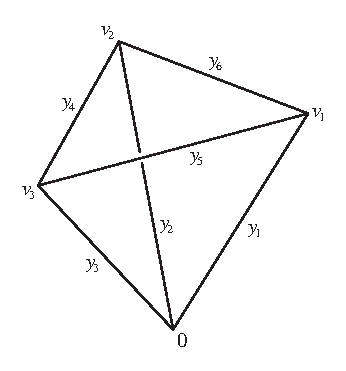
\includegraphics{PS/tet}
\end{center}
\caption{Tetrahedron with distinguished vertex and labeled edges.}
\label{fig:tet}
\end{figure}

\begin{proof}
There are three cases to consider: compression scoring, vor analytic
scoring and Voronoi scoring. This technique was introduced in
Proposition~8.7.1 of \cite{part1} for compression-scoring, and is
proved there in the compression case.

Next we consider vor analytic-scored tetrahedra.  The validity of
the same reduction for vor analytic-scored tetrahedra is obvious if
the tip of the Voronoi cell does not protrude. If the tip does
protrude, we must use the analytic continuation for the Voronoi
volume.  In this case, the validity of the reduction is not obvious.

% We provide an analytic proof (with some details omitted) that this reduction increases
% the analytic Voronoi score of a tetrahedron.
The geometric constraint of moving a vertex along an edge
can easily be stated analytically in terms of the original edge
lengths, $(y_1, y_2, y_3, y_4, y_5, y_6)$.
This action depends on a single parameter, the
distance of the vertex $v_1$ from the origin, which we call $t$.
The new edge lengths are given by
\[
( t, y_2, y_3,
  y_4,\sqrt{{t^2} + {{{y_3}}^2} -
   {\frac{t\,\left( {{{y_1}}^2} +
         {{{y_3}}^2} - {{{y_5}}^2}
         \right) }{{y_1}}}},
  \sqrt{{t^2} + {{{y_2}}^2} -
   {\frac{t\,\left( {{{y_1}}^2} +
         {{{y_2}}^2} - {{{y_6}}^2}
         \right) }{{y_1}}}} ).
\]

Recall from Section~8.6.3 of \cite{part1} that the formula for the
analytic Voronoi volume is a rational function of $\chi$, $u$,
$\sqrt{\Delta}$, and $x_i$, where $x_i = y_i^2$.  Further recall
that $\chi$, $u$, and $\Delta$ are all polynomial functions in $x_i$
that are defined in Sections~8.1 and 8.2 of \cite{part1}.

Substituting the computed edge lengths in the formula for the analytic
Voronoi volume, taking the partial derivative with
respect to $t$, replacing $t$ with $y_1$, multiplying by the positive
term
\[
8 \sqrt{\Delta} u(x_1, x_3, x_5) u(x_1, x_2, x_6)/y_1,
\]
and then simplifying, we end up with a large homogeneous
polynomial in $x_i$ of degree 6, which is too ugly to exhibit here (having
91 terms).

Evaluating this polynomial over all possible
\qrtets\ and quarters, we find that it is positive.

Therefore the volume is increasing in $t$, so to increase the score,
we should push the vertex in along the edge. The verification of the
sign of the polynomial is found in Calculation~\ref{d:dimred}. This
completes the case of vor analytic-scored tetrahedra.

The final case is Voronoi scoring.  The deformation does not change
the solid angle of the tetrahedron.  The only term of the Voronoi
score that changes is a negative constant times a volume. The
contraction of the tetrahedron decreases this volume, and increases
the score. The validity of a similar reduction argument for Voronoi
scoring of a tetrahedron is now obvious.
\end{proof}


\section{Proof of Proposition~\ref{prop:qrtetbound}}
%\section{Quasi-regular Tetrahedra}
%Otherwise known as the pentahedral cap.
% \subsection{Quasi-regular Tetrahedra}

%     Add at beginning a new paragraph: "It suffices to prove
%  Proposition 15.2 for strict PC pentahedral prisms. For each
%  non-strict PC pentahedral prism is a pointwise limit of strict
%  ones of the same combinatorial type, so the inequality in
%  the conclusion of the proposition will hold for non-strict
%  PC pentahedral prisms by continuity."

    It suffices to prove
 Proposition~\ref{prop:qrtetbound} for strict PC pentahedral prisms. Each
 non-strict PC pentahedral prism is a pointwise limit of strict
 ones of the same combinatorial type, so the inequality in
 the conclusion of the proposition will hold for non-strict
 PC pentahedral prisms by continuity.

We use three separate computations to construct and prove Proposition~\ref{prop:qrtetbound}.
First, we prove a relation between dihedral
angle and score.  We then show that if the dihedral angle of a
tetrahedron in a pentahedral cap exceeds a certain bound,
then the associated pentahedral prism is not a strict PC pentahedral prism.
% the score of the pentahedral cap must fall below $3.48 \myscorept$,
% hence such arrangements may be discarded.
% falling into the purview of Proposition~\ref{prop:pentscorebd}.
We call such a bound a
{\em dihedral cutoff}.  This cutoff allows us to prove the final bound.

%  Replace "cannot contravene." with "is not a strict PC pentahedral prism."

In the following discussion, $\dih(T)$ refers to the dihedral angle
associated with the first edge of a \qrtet\ $T$, $\myscore(T)$ refers to
the compression score of the tetrahedron,
and $\sol(T)$ refers to the solid
angle at the distinguished vertex.  We restrict
our attention to \qrtets\ whose score exceeds $-0.52 \myscorept$, as
otherwise the associated pentahedral prism cannot contravene.
% per Proposition~\ref{prop:pentscorebd}.

The first relation is
%$$\myscore(T) \le a_1 \dih(T) - a_2$$
\begin{eqnarray}
\myscore(T) \le a_1 \dih(T) - a_2  \label{eq:qr:dihrel}
\end{eqnarray}

where $a_1 = 0.3860658808124052$ and $a_2 = 0.4198577862$.
Calculation~\ref{qr:dihrel}
provides the verification of this relation.

%smside2[tt_]:= -0.4198577860315257 + 0.3860658808124052*tt

% If a pentahedral prism has a  pentahedral cap that contains
%  a quasi-regular tetrahedron with dihedral angle dih(T) \ge d_0,
%  where d_0=1.4674, then it is not a strict PC pentahedral prism."

\begin{lem}
\label{lem:dihcut}
If a pentahedral prism has a pentahedral cap that contains a \qrtet\ $T$ with
dihedral angle $\dih(T) \ge d_0$,
where $d_0 = 1.4674$, then it is not a strict PC pentahedral prism.
% we can discard it via Proposition~\ref{prop:pentscorebd}.
\end{lem}

\begin{proof}
Applying relation (\ref{eq:qr:dihrel}) to four \qrtets\ $T_i$ forming part of a strict PC pentahedral
prism, we find
\begin{eqnarray}
\sum_{i=1}^4 \myscore(T_i) \le a_1 \sum_{i=1}^4 \dih(T_i) - 4 a_2 \label{eq:qr:dihsum}
\end{eqnarray}
Applying the relation
\begin{eqnarray}
\dih(T_5) = 2 \pi - \sum_{i=1}^4 \dih(T_i) \label{eq:qr:dihsum2}
\end{eqnarray}
and adding $\myscore(T_5)$ to both sides of relation (\ref{eq:qr:dihsum}),
we find
\begin{eqnarray}
\sum_{i=1}^5 \myscore(T_i) \le \myscore(T_5) + a_1 (2 \pi - \dih(T_5)) - 4 a_2 \label{eq:qr:dihsum3}
\end{eqnarray}
The left-hand side represents the score of the pentahedral cap.
If the right-hand side does not exceed $3.48 \myscorept$,
then the pentahedral prism is not a strict PC pentahedral prism.
% Proposition~\ref{prop:pentscorebd} implies that the associated
% pentahedral prism cannot contravene.
 % (line 9) replace "Proposition 15.1 implies... cannot contravene."
 % with: " then the pentahedral prism is not a strict PC pentahedral prism.

% we can remove the arrangement from consideration,  as per Proposition~\ref{prop:pentscorebd}.

%d_0 = 1.4674

We assert that if $\dih(T) \ge d_0$,
the right-hand side
\[
\myscore(T_5)  + a_1 (2 \pi - \dih(T_5)) - 4 a_2
\]
does not exceed $3.48 \myscorept$.  Equivalently,
we prove that
$\dih(T) \ge d_0$ implies
\[
\myscore(T) - a_1 \dih(T) \le 3.48 \myscorept - 2 \pi a_1 + 4 a_2
\]
which is verified in Calculation~\ref{qr:dihcut}.

We conclude that if $\dih(T) \ge d_0$
 then the pentahedral prism cannot be a strict PC pentahedral prism.

\end{proof}

Hence we may restrict our attention to \qrtets\ whose
dihedral angle does not exceed the dihedral cutoff $d_0$.

Using the dihedral cutoff, we establish the final relation,
\[\myscore(T) + m \sol(T) + a (\dih(T) - \frac{2 \pi}{5}) - b_c \le 0\]
via Calculation~\ref{qr:pentacap}.  This completes the proof of Proposition~\ref{prop:qrtetbound}.

\section{Proof of Proposition~\ref{prop:quadbound}: Top level}

 It suffices to prove
 Proposition\ref{prop:quadbound} for strict PC pentahedral prisms,
 by a similar argument to that used for Proposition~\ref{prop:qrtetbound}.

Recall from Definition~\ref{def:standard-cluster}\tomcite{}
%of \cite{dcg2}
that a quad cluster is
a standard region that is a quadrilateral.
Quad clusters can be classified as follows:

\begin{enumerate}
 \item Flat quad clusters \label{enum:class:flat}
 \item Octahedra \label{enum:class:octa}
 \item Pure Voronoi quad clusters \label{enum:class:vor}
 \item Mixed quad clusters \label{enum:class:mixed}
\end{enumerate}

We will subdivide (\ref{enum:class:vor}) into acute and obtuse types.
See Section~\ref{sec:bounds}\tomcite{} %of \cite{dcg3} 10.4
for a discussion on the classification of quad clusters.
% make sure these references match up, as per Jeff's comments
By Lemma~\ref{lemma:1.04}\tomcite{}, the score of a mixed quad
cluster is less than $-1.04 \myscorept$. A PC pentahedral prism
therefore cannot contain a mixed quad cluster, so the bound of
Proposition~\ref{prop:quadbound} holds trivially for this class.

We treat the remaining classes in the following sections.

\section{Proof of Proposition~\ref{prop:quadbound}: Flat quad clusters}

Recall that a {\em flat} quarter is a quarter whose long edge is opposite its distinguished vertex.

\begin{lem}
\label{lem:flatquarterbd}
Given a flat quarter $Q$ with $\myscore(Q) \ge -1.04 \myscorept$, the relation
\begin{eqnarray}
\myscore(Q) \le -m \sol(Q) + b/2  \label{rel:flatquarterbd}
\end{eqnarray}
holds.
\end{lem}

\begin{proof}
Label the diagonal of a flat
quarter $y_6$.

Flat quarters may be scored using either compression or vor
scoring.  We treat each case separately.

First, suppose that we wish to prove the bound for compression scored
quarters.  This means that the circumradii of the two faces adjacent
to the long diagonal do not exceed $\sqrt{2}$.  We subdivide the
verification into
Calculation~\ref{flat:gma:dimred},
a computation where we apply dimension-reduction
and partial derivative information, and
Calculation~\ref{flat:gma:bdry}, a boundary verification, where
we restrict our attention to cells which lie on the boundary between
compression and vor scoring.

%Calculation~\ref{flat:gma:dimred} provides the verification
%of the dimension-reduction
%case.  Calculation~\ref{flat:gma:bdry} provides the
%verification of the boundary case.

Second, we treat the vor-scoring case.  In this case we prove the
bound for vor-scored quarters.  This means that at least one of
the circumradii of the two faces adjacent to the long diagonal
is at least $\sqrt{2}$.  This verification is somewhat more complex
than the compression case.  We subdivide the verification into
\begin{enumerate}
\item
Verification that the first three partials are negative on a
small cell containing the corner (Calculation~\ref{flat:partials}).
\item
Verification of the bound on that small cell containing the corner,
using the property that the first three partials are negative
(Calculation~\ref{flat:corner}).
\item
A computation where we apply dimension-reduction and partial
derivative reduction, omitting the corner cell
(Calculation~\ref{flat:vor:dimred}).
\item
A boundary verification, where we restrict our attention to
cells which lie on the boundary between compression and vor
scoring, again omitting the corner cell
(Calculation~\ref{flat:vor:bdry}).
\end{enumerate}

These calculations complete the proof of Lemma~\ref{lem:flatquarterbd}.
\end{proof}

We are now prepared to prove Proposition~\ref{prop:quadbound} for flat quad clusters.

Flat quad clusters are composed of two flat quarters, whose common face
includes the long edge.

By Proposition~\ref{prop:pentscorebd}, we restrict our attention to
flat quarters whose score exceeds $-1.04 \myscorept$, recalling the
fact that the score of flat quarters is nonpositive.

Invoking Lemma~\ref{lem:flatquarterbd} for each flat quarter and adding the relations,
we arrive at the desired
bound for flat quad clusters.  This completes the proof.

%These verifications are contained in Calculations (ref.).

\section{Proof of Proposition~\ref{prop:quadbound}: Octahedra}

% \subsection{Octahedra}
%Four upright quarters, arrayed around their common long edge so
%that each face containing the common edge is shared by two quarters,
%form an {\em octahedron}, another type of quad cluster.

Recall that quartered octahedra, a type of quad cluster,
are composed of four upright
quarters arrayed around their common long edge
(called the {\em diagonal}) so that each
face containing the common edge is shared by two quarters.

We are required to prove a relation of the form
\[ \myscore(H) + m \sol(H) - b \le 0, \]
where $\myscore(H)$ denotes the score of an octahedron $H$, $\sol(H)$ denotes
the solid angle associated with the distinguished vertex, and $m$
and $b$ are positive constants.  By Proposition~\ref{prop:pentscorebd},
we restrict our attention to
octahedra whose score exceeds $-1.04 \myscorept$.

Our treatment of octahedra, as usual, is comprised of a number of auxiliary
computations.  We prove bounds on upright quarters which are part of an
octahedron, and then combine these bounds to deduce the required bound on
octahedra in general.

The scoring function $\myscore(\cdot)$ for upright quarters is either compression
(denoted by $\gma(\cdot)$) or
an average of two $\vor(\cdot)$ scores, which we will continue to refer to as
vor-scoring.
See Remark 7.23 for a simplified version of the scoring rules.

Due to the complex nature of octahedra, we
consider a number of sub-cases.
These cases are partitioned according to the length
of the diagonal and the scoring system applied to the upright quarters.

Using a dihedral summation argument, we will eliminate octahedra
whose diagonal lies in the range $[2.51, 2.716]$.

Next, we will treat
the case where the diagonal lies in the range $[2.716, 2\sqrt{2}]$.
Using a dihedral correction term,
we will prove the bound for octahedra which are completely
compression-scored, and octahedra which are completely vor-scored.

The remaining cases will consist of
octahedra which contain either two or three
vor-scored quarters.  (Since a quarter is vor-scored if one
of the faces containing the diagonal has circumradius $\sqrt{2}$ or
greater, it is not possible for an octahedron to contain only one
vor-scored quarter.)  We treat these cases using an additional
correction term.

In all computations involving octahedra,
we label the diagonal $y_1$.

In order to simplify the computations,
we first prove an auxiliary cutoff bound.
This first bound reduces
the size of the cell over which we must conduct our search,
as per Proposition~\ref{prop:pentscorebd}.

\begin{lem}
\label{lem:octa:peel} If an upright quarter contains an edge
numbered 2, 3, 5, or 6 whose length is not less than $2.2$, its
score is less than or equal to $-0.52 \myscorept$.
\end{lem}

\begin{proof}
This is Calculation~\ref{octa:peel}.
\end{proof}

Since such an edge is shared by another upright quarter
in the same octahedron, the score of the
associated octahedron must fall below $-1.04 \myscorept$.

We restrict our search accordingly.

%Octahedral cutoff:  show that if the diagonal of an
%octahedron lies in the range [2.51,2.71], the score of
%the octahedron is less than -1.04 pt.  Hence, we can
%discard such arrangements.
%Specifically, we verify the following bound to within
%a tolerance of (fill_in_the_blank):
%sc < m*dih + b,
%where
%Newer version:  cutoff = 2.716,
%{m, b} = {-0.1533667634670977, 0.2264803995076098}
%Required tolerance (for the new bound):  3.0e-5

\begin{lem}
\label{lem:octa:2716}
The score of an octahedron $H$ with upright diagonal in the range $[2.51, 2.716]$
is less than or equal to $-1.04 \myscorept$.
\end{lem}

\begin{proof}
In Calculation~\ref{octa:cut},
we prove a bound of the form
\[
\myscore(S) + c \dih(S) \le d
\]
on upright quarters $S$, where $c = 0.1533667634670977$, and
$d = 0.2265$.  Adding the bound for four quarters $S_i$ forming
an octahedron, we find
\[
\sum_{i=1}^4 \myscore(S_i) + c \sum_{i=1}^4 \dih(S_i) \le 4 d.
\]
Using the fact that the sum of the dihedral angles is $2 \pi$,
we find that
\[
\myscore(H) \le -2 \pi c + 4 d
\]
for such an octahedron $H$.

A computation involving the constants $c$ and $d$ shows that the
score is less than $-1.04 \myscorept$.
\end{proof}

Again invoking
Proposition~\ref{prop:pentscorebd}, we need only
consider octahedra whose diagonal lies in the range
$[2.716, 2\sqrt{2}]$.

%Next, we consider octahedra which contain (at least two)
%vor-scored quarters whose diagonal falls in the range
%$[2.716, 2.81]$.  We prove a cutoff bound, showing that
%a vor-scored quarter with such a diagonal must score
%less than $-0.52 \myscorept$.  Since there must be at least
%two such quarters if there are any, the score of the
%octahedron with which they are associated must fall below
%$-1.04 \myscorept$.  We therefore discard such arrangements,
%restricting our attention to diagonals in the range

Using this assumption, we prove bounds of the form
\begin{equation}
%\[
\myscore(S) + m \sol(S) + \alpha \dih(S)  \le \frac{b}{4} +
    \alpha \frac{\pi}{2}
%\]
\label{octa:dih}
\end{equation}
and
\begin{equation}
%\[
\myscore(S) + m \sol(S) + \alpha \dih(S) + \beta x_1 \le \frac{b}{4} +
    \alpha \frac{\pi}{2} + 8 \beta,
%\]
\label{octa:edge}
\end{equation}
where $\dih(S)$ refers to the dihedral angle associated with the diagonal,
$\myscore(S)$ refers to the scoring scheme appropriate for a
particular upright quarter $S$, and $x_1$ refers to the square of the length of
the diagonal.  We
choose $\alpha$ and $\beta$ according to the scoring scheme.

Appropriate values for the correction terms involving
$\alpha$ and $\beta$ were determined by experimentation.

%For the first inequality, we choose $\alpha = 0.14$ for compression-scored
%quarters, and $\alpha = 0.054$ for vor-scored quarters.

%We prove Relation~\ref{octa:dih} for compression-scored quarters, choosing
%$\alpha = 0.14$.

Choosing $\alpha = 0.14$, we prove (\ref{octa:dih}) for compression-scored
quarters with diagonal in the interval $[2.716, 2\sqrt{2}]$
(Calculation~\ref{octa:gma:dih}).  Using
the same $\alpha$, we prove (\ref{octa:dih}) for vor-scored
quarters with diagonal in the range $[2.716, 2.81]$ (Calculation~\ref{octa:vor:dih}).

Choosing $\alpha = 0.054$, $\beta = 0.00455$, we prove (\ref{octa:edge}) for
compression-scored quarters with diagonal in $[2.81, 2\sqrt{2}]$
(Calculation~\ref{octa:gma:corr}).  Choosing
the same $\alpha$, but $\beta = -0.00455$, we prove (\ref{octa:edge}) for
vor-scored quarters with diagonal in $[2.81, 2\sqrt{2}]$
(Calculation~\ref{octa:vor:corr}).

%For the second inequality, we choose $\alpha = 0.054$, and we choose
%$\beta = 0.00455$ for compression-scored quarters, and $\beta = -0.00455$
%for vor-scored quarters.

Note that for vor-scored quarters,
the first inequality is a relaxation of the second, since $\beta$ is
negative.

The verification of each of these inequalities involves
a computation where we apply dimension-reduction
and partial derivative information, and
a boundary verification, where
we restrict our attention to cells which lie on the boundary between
compression and vor analytic scoring.
Note that the
dimension-reduction step for relation~(\ref{octa:edge}) is complicated
by the presence of the $\beta x_1$ term.


\begin{lem}
\label{lem:octabound}
Proposition~\ref{prop:quadbound} holds for octahedra with upright diagonals
in the range $[2.716, 2\sqrt{2}]$.
\end{lem}
\begin{proof}
Summing inequality (\ref{octa:dih}) over the four quarters $S_i$ of an octahedron, we find
\[
\sum_{i=1}^4 \myscore(S_i) + m \sum_{i=1}^4 \sol(S_i) + \alpha \sum_{i=1}^4 \dih(S_i)
\le b + 2 \alpha \pi.
\]
Using the fact that the dihedral angles sum to $2 \pi$, we find
\[
\myscore(H)  + m \sol(H) \le b,
\]
so octahedra $H$ with diagonals in the range $[2.716,2.81]$
satisfy the requisite bound.

Summing inequality (\ref{octa:dih}) over a consistently scored octahedron
(either all compression or all vor) with diagonal in the
range $[2.81, 2\sqrt{2}]$, we again arrive at the desired bound.

The remaining cases involve octahedra which contain both compression
and vor-scored quarters, and whose diagonals lie in the range
$[2.81, 2\sqrt{2}]$.  For this case, we use inequality (\ref{octa:edge}).

The summation involving inequality (\ref{octa:edge}) is identical to
inequality (\ref{octa:dih}) save for
the presence of the $\beta$ terms.  If there are two vor-scored
quarters and two compression-scored quarters, the beta terms cancel,
giving the relation as before.

If there are three vor-scored quarters and one compression-scored
quarter, we note that the same relation for vor-scored quarters
holds if we replace $\beta$ by $\beta/3$ (since we have now relaxed
the bound).  Summing the inequalities, the term involving $\beta$
vanishes again, leaving the desired inequality.
\end{proof}

Lemmas \ref{lem:octa:2716} and \ref{lem:octabound} prove
Proposition~\ref{prop:quadbound} for octahedra.

\section{Proof of Proposition~\ref{prop:quadbound}: Pure Voronoi quad clusters}
% \section{Pure Voronoi quad clusters}

% \subsection{Pure Voronoi quad clusters}
The next class of quad clusters which we treat are the pure
Voronoi quad clusters.  We will define a truncation operation
on these quad clusters.  Truncation will simplify the geometry of
the quad clusters, and will provide a convenient scoring bound.
We will divide our treatment of pure Voronoi quad clusters
into two cases in order to simplify the analysis and numerical
verifications as much as possible.

Recall from the classification of quad clusters
that a pure Voronoi quad cluster consists of the intersection of a
$V$-cell at the origin with the cone at the origin over a quadrilateral
standard region.  We refer to the restriction of the $V$-cell to the
cone over the quadrilateral as either the $V$-cell
or the Voronoi cell of the quad cluster.
Figure~\ref{fig:vor} describes the geometry of a simple
$V$-cell.

\begin{figure}
\begin{center}
\includegraphics{PS/vor}
\end{center}
%\centerline{ \psfig{file=vor.eps} }
\caption{A pure Voronoi quad cluster.}
\label{fig:vor}
\end{figure}

In addition, recall that a vertex lying in the cone over a pure
Voronoi quad cluster must have height greater than $2\sqrt{2}$.
Such vertices can significantly complicate the geometry of the $V$-cell,
affecting its shape and volume.

We remove the effect of vertices lying above a pure Voronoi quad cluster
by removing all points from the $V$-cell which have height greater than
$\sqrt{2}$.  We call this operation {\em truncation at} $\sqrt{2}$.
Truncation decreases the volume of the quad cluster.  This decrease in
volume increases the score of the quad cluster, bringing it closer to
the proposed bound.

We refer to truncated pure Voronoi quad clusters as {\em truncated} quad
clusters.

We define a scoring operation on pure Voronoi quad clusters which we
call {\em truncated Voronoi} scoring.  This operation consists of
truncation at $\sqrt{2}$, followed by the usual Voronoi scoring.

Each diagonal across the face of a cluster must have length
greater than $2\sqrt{2}$, otherwise we could form two flat quarters,
contradicting the decomposition.  We choose the shorter of the two
possible diagonals, and will consider that diagonal in the analysis
which follows.

We decompose the cluster into two tetrahedrons along the chosen
diagonal.  The face dividing the tetrahedrons is either acute or
it is obtuse.  We treat each case separately.

We must prove
\[
\myscore(Q) + m \sol(Q) - b \le 0,
\]
where $\myscore(Q)$ denotes the score of a pure Voronoi quad cluster $Q$, $\sol(Q)$ denotes
the solid angle associated with the distinguished vertex, and $m$
and $b$ are positive constants.
We call this relation a {\em bound} on the solid angle and score of a quad
cluster.
Invoking Proposition~\ref{prop:pentscorebd},
we restrict our attention to
quad clusters whose score exceeds $-1.04 \myscorept$.

% \subsubsection{The acute case}
% \subsection{The acute case}
% \section{Proof of Proposition~\ref{prop:quadbound}: Pure Voronoi quad clusters (acute)}
\section{Pure Voronoi quad clusters:  acute case}
\begin{lem}
\label{lem:pure:half} If an acute quad cluster is divided along an
acute separating face, then the score of each half is nonpositive.
\end{lem}
\begin{proof}
This is a consequence of the arguments of
Theorem~\ref{lemma:quad0}\tomcite.
\end{proof}

We therefore restrict our attention to halves whose score exceeds
$-1.04 \myscorept$, by Proposition~\ref{prop:pentscorebd}.

If the separating face is acute, we prove
\begin{equation}
\myscore(S_i) + m \sol(S_i) - b/2 \le 0 \label{rel:acute}
\end{equation}
for each half $S_i$
independently, and deduce the desired bound by adding the bounds
for each half.

\begin{lem}
\label{lem:pure:solid}
Let $T_0$ denote the tetrahedron with edge lengths $(2,2,2,2,2,2\sqrt{2})$.  Let
$\sol(T_0)$ denote the solid angle of the tetrahedron $T_0$.
Given a tetrahedron $T$, if $\sol(T) < \sol(T_0)$, then relation~(\ref{rel:acute}) holds.
\end{lem}
\begin{proof}
If $\sol(T) < \sol(T_0)$, then
$m \sol(T) < m \sol(T_0)$, hence
\[m \sol(T) -b/2 < m \sol(T_0) - b/2 \le 0,\]
and
\[\myscore(T) + m \sol(T) -b/2 < \myscore(T) \le 0,\]
by Lemma~\ref{lem:pure:half}.
\end{proof}

We therefore
may restrict our attention to halves whose solid angle is at least
$\sol(T_0)$.  In addition, we restrict our attention to halves for
which the dividing face is acute.

\begin{lem}
\label{lem:pure:acute}
The relation \[\myscore(T) + m \sol(T) - b/2 \le 0\] holds for a
tetrahedron $T$ forming  half of an acute quad cluster with
score exceeding $-1.04 \myscorept$.
\end{lem}
\begin{proof}
The required verifications for each half of an acute quad cluster
are somewhat difficult to achieve
directly, so we subdivide into a number of different cases
in an attempt to reduce the complexity of
the calculations.  First, we show that the bound holds for
all halves whose diagonal is at least $2.84$
(Calculation~\ref{acute:cut}).
Using this information, we then prove the
bound everywhere but in a small corner cell
(Calculation~\ref{acute:vor}).  We then restrict our
attention to the small corner cell (Calculation~\ref{acute:corner}).
These computations involve
the use of partial derivative information, and include the required
boundary computations.
\end{proof}

Invoking Lemma~\ref{lem:pure:acute} for each half and adding them proves
Proposition~\ref{prop:quadbound} for the acute case.

\section{Pure Voronoi quad clusters:  obtuse case}
% \section{Proof of Proposition~\ref{prop:quadbound}: Pure Voronoi quad clusters (obtuse)}
% \subsection{The obtuse case}
% \subsubsection{The obtuse case}
If the separating face is obtuse, the analysis becomes significantly
harder.  It is no longer possible to prove the desired bound on each
half independently.  The dimension of the full bound, even using
the usual dimension-reduction techniques, is too high to make the
verification tractable numerically.  Therefore we adopt a different
approach.

Using the dimension-reduction technique, we push each vertex along its
edge until the distance from each vertex to the origin is $2$.
We call the resulting quad cluster a {\em squashed} cluster.  Observe
that the solid angle of the cluster is unchanged, while the volume of
the Voronoi cell has decreased, thereby increasing the score of the
cluster.

Since
the central face is still obtuse, the length of the diagonal after
this perturbation must still exceed $2\sqrt{2}$.  Note, however,
that the other edge lengths in the quad cluster can be as small as
$4/2.51$.

The geometry of the $V$-cell of a squashed cluster, assuming that
there is no truncation from vertices of the packing lying above the quad
cluster, is that of Figure~\ref{fig:vor}.  When the $V$-cell is
truncated at $\sqrt{2}$ from the origin, two potential arrangements
arise.  In the first arrangement, the truncated region is connected,
as in Figure~\ref{fig:vor3}.  In second potential arrangement, the
truncated region is formed of two disjoint pieces,
as in Figure~\ref{fig:vor2}.

\begin{figure}
\begin{center}
\includegraphics{PS/vor3}
\end{center}
%\centerline{ \psfig{file=vor3.eps} }
\caption{A typical truncated quad cluster.}
\label{fig:vor3}
\end{figure}

\begin{figure}
\begin{center}
\includegraphics{PS/vor2}
\end{center}
%\centerline{ \psfig{file=vor2.eps} }
\caption{An impossible arrangement.}
\label{fig:vor2}
\end{figure}

\begin{lem}
\label{lem:pure:disjoint}
The disjoint case cannot arise for squashed quad clusters.
\end{lem}
\begin{proof}
Suppose that it could.  Pick an untruncated point
along the central ridge of the $V$-cell (see Figure~\ref{fig:vor2}).
The distance of this point
from the origin is then less than $\sqrt{2}$, but due to its location
on the central ridge, it is equidistant from the two nearest vertices
and the origin.  This implies that the circumradius of the resulting
triangle must be less than $\sqrt{2}$, which contradicts the fact
that the diagonals have length at least $2\sqrt{2}$.
\end{proof}


\subsection{A geometric argument}
% \subsubsection{A geometric argument}
We introduce a simplification which will reduce the complexity of
the obtuse case.  This simplification will consist of a perturbation of
the upper edge lengths of a squashed quad cluster.  This perturbation
will increase the score while holding the
solid angle of the quad cluster fixed.

This simplification is based on a geometric decomposition of the
truncated Voronoi cell.  We will describe the decomposition, and
then describe a construction which will ultimately simplify the
analysis.

While our arguments will extend to treat a general
squashed and truncated Voronoi cell associated with a general
standard cluster, we restrict our attention to truncated
Voronoi cells associated with quad clusters.

To begin, we consider the decomposition of
a truncated Voronoi cell into its fundamental components.
A truncated Voronoi cell is formed of three elements:  a
central spherical section (formed by the truncation), {\em wedges} of
a right circular cone, and tetrahedrons called {\em Rogers simplices}.

We choose a representation of a truncated quad cluster composed of
the radial projection of each element to a plane passing close to
the four corners of the quad cluster.
This decomposition
is represented in Figure~\ref{fig:quad2}.

\begin{figure}
%\includegraphics{PS/quad2.eps}
\begin{center}
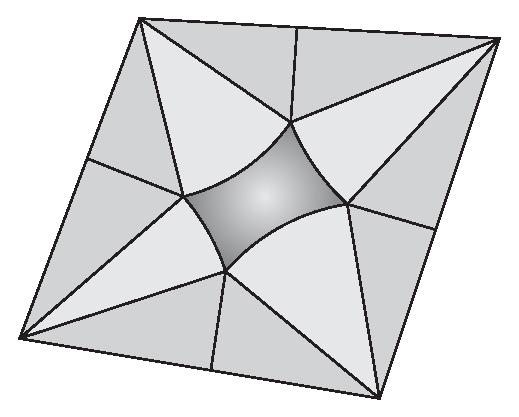
\includegraphics{PS/planar2}
\end{center}
%\centerline{ \psfig{file=quad2.eps} }
\caption{A representation of a truncated quad cluster.}
\label{fig:quad2}
\end{figure}

% \subsubsection{Rogers simplices}
\subsection{Rogers simplices}
We now consider the geometry of the Rogers simplices.

Consider a face with edge lengths $(2,2,t)$
associated with a side of
a truncated quad cluster.
Let $b$ represent the circumradius of the
face, and let $r$ represent the orthogonal extension of a
Rogers simplex from the face, as in Figure~\ref{fig:quad3}.

\begin{figure}
\begin{center}
\includegraphics{PS/quad3}
\end{center}
%\centerline{ \psfig{file=quad3.eps} }
\caption{Detail of truncated Voronoi decomposition.}
\label{fig:quad3}
\end{figure}

Then
\[
b = \frac{4}{\sqrt{16-t^2}}
\]
\[
r = \sqrt{2-b^2} = \sqrt{\frac{16-2t^2}{16-t^2}},
\]
and
\[
s = \sqrt{b^2-1} = \frac{t}{\sqrt{16-t^2}}.
\]
See Figure~\ref{fig:quad4}.

\begin{figure}
\begin{center}
\includegraphics{PS/quad4}
\end{center}
%\centerline{ \psfig{file=quad4.eps} }
\caption{Detail of Rogers simplex.}
\label{fig:quad4}
\end{figure}

\subsection{The geometric construction}
% \subsubsection{The geometric construction}
We now present the geometric construction which will imply the
simplification.

We represent the geometry of the truncated Voronoi cell associated with
one half of a quad cluster in Figure~\ref{fig:decomp1}.

\begin{figure}
\begin{center}
\includegraphics{PS/decomp1}
\end{center}
%\centerline{ \psfig{file=decomp1.eps} }
\caption{Decomposition of a truncated Voronoi cell.}
\label{fig:decomp1}
\end{figure}

We can simplify the representation by
extending the wedges to enclose the Rogers simplices.
See Figure~\ref{fig:decomp2}.
This process adds an extra volume term.

\begin{figure}
\begin{center}
\includegraphics{PS/decomp2}
\end{center}
%\centerline{ \psfig{file=decomp2.eps} }
\caption{Wedges extended to include the Rogers simplices.}
\label{fig:decomp2}
\end{figure}

The overlap between the wedges is slightly complicated.  We
simplify the overlap as follows.  Take the cone over the overlap.
Intersect it with a ball of radius $\sqrt{2}$ at the origin.
We call the spherical sections produced by this construction
{\em flutes}.  This construction is represented in
Figure~\ref{fig:decomp3}.  Figure~\ref{fig:planar3}
is a planar representation of this construction.

\begin{figure}
\begin{center}
\includegraphics{PS/decomp3}
\end{center}
%\centerline{ \psfig{file=decomp3.eps} }
\caption{Decomposition with flutes.}
\label{fig:decomp3}
\end{figure}

\begin{figure}
\begin{center}
\includegraphics{PS/planar3}
\end{center}
%\centerline{ \psfig{file=planar3.eps} }
\caption{Planar representation with flutes.}
\label{fig:planar3}
\end{figure}

To form each flute, we have added two extra pieces of
volume (per flute) to our construction.
We call these pieces {\em quoins}.  We
attach each quoin to a Rogers simplex.
See Figure~\ref{fig:quad8}.

\begin{figure}
\begin{center}
\includegraphics{PS/quad8}
\end{center}
%\centerline{ \psfig{file=quad8.eps} }
\caption{Detail of Rogers simplex with quoin.}
\label{fig:quad8}
\end{figure}

% \subsubsection{A solid angle invariant}
\subsection{A solid angle invariant}
We now require some notation for the volumes which enter
into this construction.
Let $c$ denote the volume of the central spherical angle.
Let $r$ denote the volume of the Rogers simplices.
Let $w$ denote the volume of the wedges.
Let $w'$ denote the volume of the extended wedges.
Let $q$ denote the volume of the quoins.
Let $f$ denote the volume of the flutes.
Finally, let $v$ denote the volume of the truncated Voronoi cell.

\begin{lem}
\label{lem:pure:inv}
If we hold the solid angle fixed, the volume of a truncated squashed
Voronoi cell depends only on $q$, the volume of the quoins.
\end{lem}
\begin{proof}
By the original decomposition,
\[
v = c + r + w.
\]
By our construction,
\[
v = c + w' + q - f.
\]

Recall that the
solid angle $s$ of the quad cluster is the sum of the
dihedral angles minus $2\pi$.
The dihedral angles to which we refer are those
associated with the edges between each corner
of the quad cluster and the origin.

Our perturbation will hold the solid angle $s$ of the quad cluster
fixed.  Therefore,
the sum of the dihedral angles must also be fixed.
This fixes $w'$.

Take the cone over each extended wedge and intersect it with
a ball of radius $\sqrt{2}$ centered at the origin.
Let $t$ denote the sum of these volumes.  Since the sum
of the dihedral angles is fixed, $t$ is also fixed.

Further, note that
\[
\frac{2\sqrt{2}}{3} s = c + t - f.
\]
This relation implies that $c-f$ is fixed.  Combining this with
the previous relations, we find that if we hold the solid angle
fixed, the volume of the truncated Voronoi cell depends only
on $q$, the volume of the quoins.
\end{proof}

% \subsubsection{The quoin}
% \subsection{The volume of a quoin}
\subsection{Variation of the volume of a quoin}

Consider a face $(2,2,t)$ of a truncated quad cluster.
Two Rogers simplices are associated with this face, as
suggested in Figure~\ref{fig:quad3}.
Observe that the volume of the quoin associated with one
of these Rogers simplices is increasing
in $r = \sqrt{\frac{16-2t^2}{16-t^2}}$.
Next, observe that $r$ is in turn decreasing in
$t$.
Therefore increasing $t$ decreases the volume
of the squashed quad cluster, if we hold the solid angle fixed (by varying
the length of another edge of the squashed quad cluster).

Each half of a squashed quad cluster has two variable edge lengths (not counting the
shared diagonal).  We label the variable
edge lengths of one half of the squashed quad cluster $y_1$ and $y_2$.
We label the length of the diagonal $d$.
Holding the solid
angle fixed, we may perturb one half by shrinking the larger
and increasing the shorter length.
We wish to establish the following lemma, that
increasing the short length reduces the volume of the
truncated Voronoi cell
more than decreasing the longer length increases the volume.

\begin{lem}
\label{lem:pure:reduction}
Holding the solid angle fixed for one half of a squashed quad cluster,
shrinking the longer upper edge (while increasing the shorter edge appropriately)
reduces the volume of the squashed quad cluster (increasing the score).
\end{lem}

% \subsubsection{The volume of a quoin}
% \subsection{The volume of a quoin}
To prove Lemma~\ref{lem:pure:reduction}, we establish a variational formula for the volume of a
quoin.

We then verify that the volume of the quoin associated with the
shorter edge is decreasing
faster under this perturbation than the volume
of the quoin associated with the
longer edge is increasing.

In other words, we wish to show that $y_1 < y_2$ implies
that $V(y_1) + V(y_2(y_1))$ is decreasing in $y_1$, or
equivalently,
\[
V_t(y_1) + V_t(y_2(y_1)) \frac{dy_2}{dy_1} < 0
\]
where
$V(t)$ is the volume of the quoin, $V_t(t)$ is the
derivative of the volume, and $y_2$ is an implicit function
of $y_1$.

We construct the volume of a quoin by integrating the area of
a slice.  We place the quoin in a convenient coordinate system.
See Figures~\ref{fig:quoin1} and~\ref{fig:quoin2}.
The truncating sphere has equation $x^2 + y^2 + z^2 = 2$.
At the base of the quoin, $z=1$, so $x = \sqrt{1-y^2}$ gives
the location of the right-boundary of the quoin.
The plane forming the left face of the quoin is given by the
equation $x = s z$, so the ridge of the quoin is given by the
curve $(s u, y, u)$, where $u = \sqrt{\frac{2-y^2}{1+s^2}}$.

\begin{figure}
\begin{center}
\includegraphics{PS/quoin1}
\end{center}
%\centerline{ \psfig{file=quoin1.eps} }
\caption{Top view of quoin.}
\label{fig:quoin1}
\end{figure}

\begin{figure}
\begin{center}
\includegraphics{PS/quoin2}
\end{center}
%\centerline{ \psfig{file=quoin2.eps} }
\caption{Side view of quoin.}
\label{fig:quoin2}
\end{figure}

Hence the area of a slice parallel to the $x$-$z$ plane is given
by the formula
\[
A(t,y) = \frac{1}{2}(s u - s)(u - 1) +
\int_{s u}^{\sqrt{1-y^2}}{(\sqrt{2-x^2-y^2}-1) \,dx}.
\]
The volume of a quoin is therefore given by the formula
\[
V(t) = \int_0^r{A(t,y)\,dy}.
\]

We actually only need to compute $V_t(t)$,
which is fortunate,
since the explicit formula for $V(t)$ is somewhat complicated.
We have
\[
V_t(t) = \int_0^r{A_t(t,y)\,dy} + A(t,r) r_t,
\]
but $A(t,r) = 0$, so
\[
V_t(t) = \int_0^r{A_t(t,y)\,dy}.
\]
So in addition, we only need $A_t(t,y)$,
%\[
%A_t(t,y) = (\frac{s}{2}(u^2+1) - \sqrt{1-y^2} +
%\int_{s u}^{\sqrt{1-y^2}}{\sqrt{2-x^2-y^2}\,dx})_t,
%\]
\[
A_t(t,y) = (\frac{s}{2}(u^2+1) - \sqrt{1-y^2} +
\int_{\frac{t}{4}\sqrt{2-y^2}}^{\sqrt{1-y^2}}{\sqrt{2-x^2-y^2}\,dx})_t,
\]
so
\[
A_t(t,y) = (\frac{s}{2}(u^2+1))_t -
\sqrt{2-\frac{t^2}{16}(2-y^2) - y^2}\frac{1}{4}\sqrt{2-y^2}
\]
which simplifies to
\[
A_t(t,y) = \frac{8}{(16-t^2)^{3/2}} - \frac{2-y^2}{2\sqrt{16-t^2}}.
\]
Hence
\[
V_t(t) = \frac{8r}{(16-t^2)^{3/2}} - \frac{r}{\sqrt{16-t^2}} +
\frac{r^3}{6\sqrt{16-t^2}},
\]
which simplifies to
\[
V_t(t) = \frac{-2\sqrt{2}(8-t^2)^{3/2}}{3(16-t^2)^2}.
\]

% \subsection{The solid angle constraint}
% \subsubsection{The solid angle constraint}

We are now prepared to prove Lemma~\ref{lem:pure:reduction}.
\begin{proof}
Holding the solid angle fixed, $y_2$ is an implicit
function of $y_1$.
We wish to prove that $y_1 < y_2$ implies
\begin{equation}
V_t + V_t frac{dy_2}{dy_1}  0.  \label{eqn:pure:reduction:var}
\end{equation}

We derive a formula for
$\frac{dy_2}{dy_1}$, using the solid angle constraint
\begin{equation}
\sol(2,2,2,y_1,y_2,d)=c, \label{eqn:sol}
\end{equation}
where $c$ is a constant. Using formulas from \cite{part1},
(\ref{eqn:sol}) becomes
\[
2 \arctan(\frac{\sqrt{\Delta}}{2a}) = c.
\]
Let $x_1 = y_1^2$, $x_2 = y_2^2$, and $b = d^2$.  Then
\[
\Delta = -4b^2 -4(x_1-x_2)^2 + b(x_1(8-x_2) + 8x_2),
\]
and
\[
a = 32 - d - x_1 - x_2.
\]
So
\[
\frac{-4b^2 -4(x_1-x_2)^2 + b(x_1(8-x_2) + 8x_2)}{(32 - d - x_1 - x_2)^2} = c_1.
\]
Therefore
\[
\frac{dx_2}{dx_1} = -\frac{(16-x_2)(x_2 + b - x_1)}{(16-x_1)(x_1 + b - x_2)},
\]
and
\[
\frac{dy_2}{dy_1} = \frac{y_1}{y_2} \frac{dx_2}{dx_1},
\]
hence
\begin{equation}
\frac{dy_2}{dy_1} = -\frac{y_1(16-x_2)(x_2 + b - x_1)}{y_2(16-x_1)(x_1 + b - x_2)}. \label{eqn:pure:reduction:deriv}
\end{equation}

We substitute the formula for $\frac{dy_2}{dy_1}$ into (\ref{eqn:pure:reduction:var}).
Letting $x_i = y_i^2$, and noting that all the denominators are positive,
we obtain on clearing denominators that the desired relation (\ref{eqn:pure:reduction:var})
is equivalent to

\begin{eqnarray*}
-(8-x_1)^{3/2}(16-x_2)y_2(x_1 + b - x_2) + \\
(8-x_2)^{3/2}(16-x_1) y_1 (x_2 + b - x_1) & < & 0,
\end{eqnarray*}
or
\begin{eqnarray*}
(16-x_1)^2 x_1 (8-x_2)^3 (b - x_1 + x_2)^2 < \\
(16-x_2)^2 x_2 (8-x_1)^3 (b +x_1 - x_2)^2.
\end{eqnarray*}
If we define
\[
g(x_1,x_2) = (16-x_1)^2 x_1 (8-x_2)^3 (b - x_1 + x_2)^2,
\]
then the
desired inequality is equivalent to
$g(x_1,x_2) < g(x_2,x_1)$ for $x_1 < x_2$.
There are several ways to prove this monotonicity relation.
One is to prove that the
polynomial
\[
\frac{g(x_1,x_2)-g(x_2,x_1)}{8(x_1-x_2)}
\]
is positive for all allowable values for $x_1$, $x_2$, and $b$.  Unfortunately, the
resulting polynomial has degree $6$, so the verification is somewhat unwieldy,
although easy enough using interval methods.

A simpler method involves a factorization of $g$ into
$g_1$ and $g_2$.  We show that $g_1$ and $g_2$ each
satisfy the monotonicity relation, and the relation then follows for $g$.

Define
\[
g_1(x_1,x_2) = (16-x_1) x_1 (8-x_2) (b-x_1+x_2),
\]
and
\[
g_2(x_1,x_2) = (16-x_1)(8-x_2)^2(b-x_1+x_2).
\]
Clearly
$g = g_1 g_2$.  We then construct the polynomials
\[
p_1 = \frac{g_1(x_1,x_2) - g_1(x_2,x_1)}{x_1-x_2}
\]
and
\[
p_2 = \frac{g_2(x_1,x_2) - g_2(x_2,x_1)}{x_1-x_2}.
\]

Simplifying $p_1$ and $p_2$, we find that
\begin{align*}
p_1 = & 128b - 128x_1 -8b x_1 + 8 x_1^2 - 128 x_2 \\
    & + 32 x_1 x_2 + b x_1 x_2 -x_1^2 x_2 + 8 x_2^2 - x_1 x_2^2
\end{align*}
and
\begin{align*}
p_2 = & -2048 + 192b + 320x_1 -16b x_1 -16x_1^2 +
    320x_2 \\ & - 16b x_2 -32 x_1 x_2 +b x_1 x_2 +
    x_1^2 x_2 - 16x_2^2 + x_1 x_2^2.
\end{align*}
These polynomials are quadratic in $x_1$ and $x_2$,
and linear in $b$.  The coefficient of $b$ in $p_1$
is
\[
128 -8x_1 -8x_2 + x_1 x_2.
\]
The coefficient of $b$ in $p_2$ is
\[
192 - 16x_1 -16x_2 + x_1 x_2.
\]
Both coefficients are positive for
$x_1$ and $x_2$ in $[16/2.51^2,2.51^2]$.  Therefore, the
minimum values of $p_1$ and $p_2$ occur
when $b$ is at a minimum, $b=8$.

The minimum value of each polynomial
for values of $x_1$ and $x_2$ in the range $[16/2.51^2,2.51^2]$
is now easily computed.
Making the appropriate computations, we find that each polynomial
is indeed positive.  Hence the desired relation follows.
\end{proof}

% \subsubsection{The simplification}
\subsection{Final simplification}
\begin{lem}
\label{lem:pure:obtuse}
Obtuse quad clusters satisfy the bound of Proposition~\ref{prop:quadbound}.
\end{lem}
\begin{proof}
We begin with a squashed quad cluster with consecutive upper
edge lengths $(y_1,y_2,y_3,y_4)$ and diagonal $d$ adjacent to
the first two upper edges.

Recall that we chose the diagonal of the quad cluster to be the
shorter of the two possible diagonals.  We refer to the other
possible diagonal as the {\em cross-diagonal}.
Recall that the reduction fixes the length of the diagonal.

If the length of the cross-diagonal does not drop to $2\sqrt{2}$
under the perturbation of Lemma~\ref{lem:pure:reduction}, we arrive at the configuration with
edge lengths $(y_1', y_1', y_2', y_2')$ with diagonal $d$.

If the length of the cross-diagonal does drop to $2\sqrt{2}$, then
stop the perturbation.  This gives a quadrilateral
$(y_1', y_2', y_3', y_4')$ with diagonal $2\sqrt{2}$.
Applying the perturbation to each half independently, we find
that the score of each half is maximized by the configuration
$(y_1'', y_1'', y_2'', y_2'')$ with diagonal $2\sqrt{2}$.
We verify the relation for this arrangement in
Calculation~\ref{obtuse:vor2}.

If the length of the cross-diagonal did not drop to $2\sqrt{2}$,
switch to the cross-diagonal and repeat the process.  If the
(new) cross-diagonal does not drop to $2\sqrt{2}$, we have
arrived at the configuration $(y,y,y,y)$ with diagonal $d'$.
Choose a new diagonal $d''$ to be the shorter of the two
possible diagonals.  We verify the desired relation for
this arrangement in Calculation~\ref{obtuse:vor}.

Finally, we make a few comments about extra constraints in
the verifications.

Since the score of a quad cluster is nonpositive, and $m
(2\sol(T_0)) - b \le 0$ where $\sol(T_0) = \sol( 2,2,2,2,2,2\sqrt{2}
)$, we need only consider quad clusters for which the solid angle
exceeds $2\sol(T_0)$.

The maximum length of the diagonal is $2.51 \sqrt{2}$, since
otherwise the triangles in the quadrilateral would be obtuse,
forcing the cross-diagonal to be shorter than the diagonal.
This would contradict our
original choice of the shortest diagonal.

In Calculation~\ref{obtuse:vor}, we assume that $d$ is the shortest diagonal.
Adding this constraint directly is tedious, since the
formula for the cross-diagonal of the quad cluster is somewhat
complicated.  We apply a simpler but weaker constraint,
that the diagonal $d$ of a planar quadrilateral
with edge lengths $(y,y,y,y)$ is shorter than $d'$, the other planar
diagonal.  The constraint $d \le d'$ gives the constraint $d^2 \le 2 y^2$.
Since the cross-diagonal of the quad cluster is shorter than the
cross-diagonal of the planar quadrilateral, this constraint is weaker.
\end{proof}

Lemmas \ref{lem:pure:acute} and \ref{lem:pure:obtuse} prove
Proposition~\ref{prop:quadbound} for pure Voronoi quad clusters.

\chapter{Calculations}

The verifications of the relations required in this paper
appear intractable using
traditional methods.  Therefore, we use a relatively new proof technique,
interval arithmetic via floating-point computer calculations.

\section{Interval Arithmetic}
 % Due to the complex nature of the functions $\myscore(\cdot)$, $\dih(\cdot)$, $\sol(\cdot)$, etc.,
% %  it is typically unrealistic to attempt to prove the required relations directly.  Instead,
% we prove the majority of the relations via
% computer-based interval arithmetic methods.

We review the basic notions of interval arithmetic.

Suppose that the value of a function $f(x)$ lies in the interval
$[a,b]$.  Further, suppose that $g(x)$ lies in the interval $[c,d]$.
Then $f(x) + g(x)$ must lie in $[a+c,b+d]$.  While it may be the case
that we could produce better bounds than this for the function $f + g$,
these interval bounds give crude control over the behavior of the
function.  Interval arithmetic provides a mechanism for formalizing
arithmetic on these bounds.

We represent an interval $t$ as $\big[\underline{t},\overline{t}\big]$.
Then for intervals $a$ and $b$,
\[
a + b = \big[\underline{a} + \underline{b}, \overline{a} + \overline{b}\big].
\]
Likewise,
\[
a - b = \big[\underline{a} - \overline{b}, \overline{a} - \underline{b}\big].
\]
Multiplication is somewhat more complicated.  Define
\[
C = \{\underline{a} \/ \underline{b}, \underline{a} \overline{b},
    \overline{a} \underline{b}, \overline{a} \overline{b}\}.
\]
Then
\[
a*b = [\min(C), \max(C)].
\]
Division is similar, as long as the dividing interval does not contain zero.

Similarly, we can define the operation of a monotonic function on
an interval.  For example,
\[
\arctan(a) = [\arctan(\underline{a}), \arctan(\overline{a})].
\]

Using interval arithmetic, we can produce rigorous bounds for polynomials
evaluated on intervals.  Likewise, we can produce rigorous bounds for
rational functions evaluated on intervals.  Finally, we add the
composition of monotonic functions.  This allows us to produce interval
bounds for functions such as $\sol(\cdot)$ and $\vor(\cdot)$ over \qrtets,
quarters, or quad clusters.


\section{The Method of Subdivision}
The relations on tetrahedra and quad clusters required for
our approach typically have
the form
$g(y)\le 0$ for $y \in I$, where $I$ is a product of closed
intervals.  As $g$ is usually continuous, the existence of a
maximum is trivial.  However, bounds on the behavior of $g$
over all of $I$ computed directly via interval arithmetic
are generally poor.

We define a {\em cell} to be a product of closed intervals.
By subdividing $I$ into
sufficiently small cells, the quality of the computed bounds on
each cell usually
improves enough to prove the relation for each cell, and hence
for the original domain $I$.

If in fact $g(y) \le c < 0$, this approach works very well.  However,
if the bound is tight at a point $y_0$, i.e., $g(y_0)=0$, then pure
subdivision will usually fail, since the computed upper bound on $g$ over
any cell containing $y_0$ will typically be positive.

If $y_0$ is not an interior maximum,
we turn to the partial derivatives of $g$.  If
we can show that the partials of $g$ on a small cell containing
$y_0$ have fixed sign (bounded away from zero), then the
maximum value of $g$ on that cell is easily computed.
It is typically the case that a cell
must be very small before we can determine the sign of the
partials via interval arithmetic bounds.


\section{Numerical Considerations}
Most real numbers are not representable in computer floating-point
format.  However, floating-point intervals may be found which contain
any real number.  Although the magnitude of real numbers representable in
fixed-length floating-point format is finite, the format also provides
for $\pm \infty$, which allows for interval containment of all reals.
These intervals may be
added, multiplied, etc., and the resulting intervals will contain
the result of the operation applied to the real numbers which they
represent.

Since floating-point arithmetic is not exact, interval arithmetic
conducted using floating-point arithmetic is not optimal, in the
sense that the interval resulting from an operation will usually
be larger than the true resultant interval, due to roundoff.
However, barring hardware or software errors (implementation errors,
not roundoff errors), floating-point
interval arithmetic, unlike floating-point arithmetic, is correct, in
the sense that it provides correct interval bounds on the value
of a computation, while floating-point arithmetic alone only
provides an approximation to the correct value of a computation.
We may therefore use interval arithmetic to prove mathematical
results.  Floating-point arithmetic alone, in the absence of
rigorous error analysis, cannot constitute a proof.

We implement floating-point interval arithmetic routines via
the IEEE 754 Standard for floating-point arithmetic \cite{IEEE}.

Implementation of interval arithmetic is straightforward using
directed rounding.  In addition to arithmetic functions, we require
interval implementations of the
square root and arctangent functions.  Fortunately, the IEEE standard
provides the square root function.  However, the arctangent function
is somewhat problematic, since the
standard math libraries do not provide explicit error bounds for their
implementations of the arctangent function.  In theory, they
should provide an accuracy for the arctangent routine of
$0.7$ ulps, meaning that the error is less than one unit in the
last place.  I add interval padding of the form
$[v-\epsilon, v+\epsilon]$,
where $v$ is the computed value, and $\epsilon = 2^{-49}$.
This should be sufficient to guarantee proper interval containment,
assuming that the library routines are correctly implemented.

Armed with standard interval arithmetic and interval arithmetic
implementations of {\em sqrt} and {\em arctan}, we can implement
interval arithmetic versions of all
the special functions required for proving the sphere packing
relations.

Evaluating these functions on cells, we get bounds.  Unfortunately,
these bounds are not very good.  The bounds which we get from
interval versions of the partial derivative functions are even
worse.  This means that cells have to be very small before we
can draw conclusions about the signs of the partials.  These bad
bounds are due to the inherent nature of interval arithmetic--it
produces worst-case results by design.

These bad bounds increase the complexity of the verifications tremendously.
Some verifications, using these bounds,
require the consideration of billions or trillions
of cells, or worse.  Therefore, we needed a method for producing
better bounds than those which direct interval methods could
provide.

The method which we eventually discovered is to use Taylor series.
We compute explicit second (mixed) partial bounds for the major
special functions, and use these bounds to produce very good
interval bounds.  These bounds are computed in
Calculations \ref{secpar:dih:qr} through \ref{secpar:vor}.
%The beauty of the Taylor series method is that the error
%enters the calculation only once, instead of compounding with
%every arithmetic operation.
Essentially, the Taylor method postpones the error bound until the
end of the computation, eliminating the error bound explosion which
occurs with a straightforward interval method implementation.


%\appendix

\section{Calculations}
The following inequalities have been proved by computer using
interval methods.  Let $S = S(y) = S(y_1,\ldots,y_6)$ denote
a tetrahedron parametrized by the edge lengths $(y_1,\ldots,y_6)$.
In addition, we often parametrize by the squares of the edge
lengths, $(x_1,\ldots,x_6)$.

Recall from Section~\ref{sec:dabound} that $m = 0.3621$, $b = 0.49246$,
$a = 0.0739626$ and $b_c = 0.253095$.

Recall that for our purposes,
the scoring function $\myscore(\cdot)$ is given by one of four functions:
$\gma(\cdot)$, $\vor(\cdot)$, $\octavor(\cdot)$, or truncated Voronoi.
% Here $\gma(\cdot)$ is the compression
% function (also known as $\Gamma(\cdot)$).
% As usual, $\vor(\cdot)$ is the score determined by the analytic continuation of the Voronoi
% volume associated with a distinguished vertex of a tetrahedron.
% We let $\octavor(\cdot)$ denote the rule
% for upright quarters not scored by compression.  This is a case of context (4,0), and
% $\octavor(\cdot)$ is an average of two $\vor(\cdot)$ scores.
See Remark~\ref{remark:score}\tomcite\ for a simplified version of
the scoring function.

The scoring rules depend on $\eta(\cdot)$, the circumradius of a
face, introduced in Definition~\ref{def:eta}\tomcite.

%Moved Dimension Reduction to end, so numbering matches better.


\subsection{Quasi-regular Tetrahedra}

Define $C = [2,2.51]^6$, and recall
\[
a_1 = 0.3860658808124052, a_2 = 0.4198577862,
d_0 = 1.4674.\]

\begin{calcf}
Either
 \[\gma(S) \le a_1 \dih(S) - a_2\]
or
 \[\gma(S) \le -0.52\myscorept\]
for $y \in C$, using dimension-reduction.
 \label{qr:dihrel}
\end{calcf}

\begin{calcf}
Either
\[\gma(S) - a_1 \dih(S) \le 3.48 \myscorept - 2 \pi a_1 + 4 a_2\]
or
\[\dih(S) < d_0\]
or
\[\gma(S) \le -0.52\myscorept\]
for $y \in C$, using dimension-reduction.
\label{qr:dihcut}
\end{calcf}

\begin{calcf}
Either
\[\gma(S) + m \sol(S) + a( \dih(S) -
\frac{2\pi}{5}) - b_c \le 0\]
or
\[\dih(S) > d_0\]
or
\[\gma(S) \le -0.52\myscorept\]
for $y \in C$, using dimension-reduction.
\label{qr:pentacap}
\end{calcf}


\subsection{Flat Quad Clusters}

Define $I = [2,2.51]^5[2.51,2\sqrt{2}]$, and define the
corner cell
\[C = [2,2 + 0.51/16]^5[2\sqrt{2} - (2\sqrt{2}-2.51)/16,2\sqrt{2}].\]

\begin{calcf}
Either
\[\gma(S) + m \sol(S) \le b/2\]
or
\[\eta(y_1,y_2,y_6)^2 > 2\]
or
\[\eta(y_4, y_5, y_6)^2 > 2\]
or
\[\gma(S) \le -1.04\myscorept\]
for $y \in I$, using dimension reduction.
\label{flat:gma:dimred}
\end{calcf}

\begin{calcf}
Either
\[\gma(S) + m \sol(S) \le b/2\]
or
\[\eta(y_1,y_2,y_6)^2 = 2 \text{~with~} \eta(y_4, y_5, y_6)^2 \le 2,\]
or
\[\eta(y_4, y_5, y_6)^2 = 2 \text{~with~} \eta(y_1,y_2,y_6)^2 \le 2,\]
or
\[\gma(S) \le -1.04\myscorept\]
for $y \in I$, not using dimension-reduction.
\label{flat:gma:bdry}
\end{calcf}

\begin{calcf}
$\frac{d}{dy_i}\vor(S) < 0$ for $i=1,2,3$ and $y \in C$.
\label{flat:partials}
\end{calcf}

%This one is tricky.  Two cases:  either the side face, (1 2 6) is large,
%or the top face, (4 5 6) is large.  In the first case,
%partials force eta(1 2 6)^2 = 2.  So solve for y1.

\begin{calcf}
This computation is somewhat tricky, since the scoring
constraint depends on both faces.  The partial derivative
information gives $y_3=2$.  The rest of the
analysis depends on which face is assumed to be large.

If the $(y_1, y_2, y_6)$ face is large, the partial derivative
information implies that the face constraint
is tight, so $\eta(y_1,y_2,y_6)^2=2$.  Therefore solve
for $y_1$ in terms of $y_2$ and $y_6$.  Apply partial
derivative information for $y_4$ and $y_5$.
In this case,
\[\vor(S) + m \sol(S) \le b/2\]
for $y_3=2$, $y \in C$.

If the $(y_4,y_5,y_6)$ face is large, assume that
$y_1=y_2=2$.  Then either
\[\vor(S) + m \sol(S) \le b/2\]
or
\[\eta(y_4,y_5,y_6)^2 < 2\]
for $y_1=y_2=y_3=2$, $y \in C$.
\label{flat:corner}
\end{calcf}

\begin{calcf}
Either
\[\vor(S) + m \sol(S) \le b/2,\]
or
\[\eta(y_1,y_2,y_6)^2 < 2 \text{~and~} \eta(y_4, y_5, y_6)^2 < 2,\]
or
\[\vor(S) \le -1.04\myscorept\]
for $y \in I$, $y \notin C$, using dimension-reduction and partial
derivative information.
\label{flat:vor:dimred}
\end{calcf}

\begin{calcf}
Either
\[\vor(S) + m \sol(S) \le b/2,\]
with
\[\eta(y_1,y_2,y_6)^2 = 2 \text{~or~} \eta(y_4, y_5, y_6)^2 = 2,\]
or
\[\vor(S) \le -1.04\myscorept\]
for $y \in I$, $y \notin C$, not using dimension-reduction.
\label{flat:vor:bdry}
\end{calcf}


\subsection{Octahedra}

\begin{calcf}
%Since each quarter in an octahedron shares
%all edges except $y_4$ with an adjacent quarter,
%if one of these edges has length at least $2.2$, the
%adjacent quarter shares that property.  We demonstrate
%that if one of these edges is at least $2.2$, the
%score of the quarter does not exceed $-0.52 \myscorept$,
%therefore the two quarters together may be discarded.
$\myscore(S) \le -0.52 \myscorept$,
for each (appropriately scored) upright quarter
with edge lengths in the cell
$[2.51,2\sqrt{2}][2.2,2.51][2,2.51]^4$.
\label{octa:peel}
\end{calcf}

\begin{calcf}
Recall $c = 0.1533667634670977$, and
$d = 0.2265$.  Either
\[\gma(S) + c \dih(S) \le d\]
or
\[\gma(S) \le -1.04 \myscorept\]
for $y \in [2.51,2.716][2,2.2]^5$, using dimension-reduction  Note that for both
faces adjacent to the diagonal,
\[\max \eta^2 = \eta(2.2,2.2,2.716)^2 < 2,\]
so all quarters in this cell are compression-scored.
\label{octa:cut}
\end{calcf}

\begin{calcf}
Either
\[\gma(S) + m \sol(S) + \alpha \dih(S)  \le \frac{b}{4} +
    \alpha \frac{\pi}{2}\]
or
\[\gma(S) \le -1.04 \myscorept\]
for all compression-scored
quarters $S(y)$, where $\alpha = 0.14$,
\[y \in [2.716,2\sqrt{2}][2,2.2]^2[2,2.51][2,2.2]^2,\]
using dimension-reduction.
\label{octa:gma:dih}
\end{calcf}

\begin{calcf}
Either
\[\octavor(S) + m \sol(S) + \alpha \dih(S)  \le \frac{b}{4} +
    \alpha \frac{\pi}{2}\]
or
\[\octavor(S) \le -1.04 \myscorept\]
for all vor analytic-scored
quarters $S(y)$, where $\alpha = 0.14$,
\[y \in [2.716,2.81][2,2.2]^2[2,2.51][2,2.2]^2.\]
\label{octa:vor:dih}
\end{calcf}

\begin{calcf}
Either
\[\gma(S) + m \sol(S) + \alpha \dih(S) +
    \beta x_1 \le \frac{b}{4} +
    \alpha \frac{\pi}{2} + 8 \beta\]
or
\[\gma(S) \le -1.04 \myscorept\]
for all compression-scored
quarters $S(y)$, where $\alpha = 0.054$, $\beta = 0.00455$,
$x_1=y_1^2$, and
\[y \in [2.81,2\sqrt{2}][2,2.2]^2[2,2.51][2,2.2]^2,\]
using some dimension-reduction.
\label{octa:gma:corr}
\end{calcf}

\begin{calcf}
Either
\[\octavor(S) + m \sol(S) + \alpha \dih(S) +
    \beta x_1 \le \frac{b}{4} +
    \alpha \frac{\pi}{2} + 8 \beta\]
or
\[\octavor(S) \le -1.04 \myscorept\]
for all vor analytic-scored
quarters $S(y)$, where $\alpha = 0.054$, $\beta = -0.00455$,
$x_1=y_1^2$, and
\[y \in [2.81,2\sqrt{2}][2,2.2]^2[2,2.51][2,2.2]^2.\]
\label{octa:vor:corr}
\end{calcf}


\subsection{Pure Voronoi Quad Clusters}

Recall $\sol(T_0)$ denotes the solid angle of the tetrahedron
$(2,2,2,2,2,2\sqrt{2})$.

Define the corner cell $C = [2, 2 + 0.51/8]^5[2\sqrt{2}, 2.84]$.
We denote truncated Voronoi scoring by $\myscore$.
The constraint that the dividing face be acute translates
into $x_1 + x_2 - x_6 \ge 0$.  In each computation we apply
dimension-reduction.

We begin with the acute case.

\begin{calcf}
Either
\[\myscore(S) + m \sol(S) - b/2 \le 0\]
or
\[\sol(S) < \sol(T_0)\]
or
\[x_1 + x_2 - x_6 < 0\]
or
\[\myscore(S) \le -1.04 \myscorept\] for
$y \in [2,2.51]^5[2.84,4]$.
\label{acute:cut}
\end{calcf}

\begin{calcf}
Either
\[\myscore(S) + m \sol(S) - b/2 \le 0\]
or
\[\sol(S) < \sol(T_0)\]
or
\[x_1 + x_2 - x_6 < 0\]
or
\[\myscore(S) \le -1.04 \myscorept\]
for
$y \in [2,2.51]^5[2\sqrt{2},2.84]$ with $y \notin C$.
\label{acute:vor}
\end{calcf}

\begin{calcf}
Either
\[\myscore(S) + m \sol(S) - b/2 \le 0\]
or
\[\sol(S) < \sol(T_0)\]
or
\[x_1 + x_2 - x_6 < 0,\]
$y \in C$.
\label{acute:corner}
\end{calcf}

Finally, we consider the obtuse case.

\begin{calcf}
Either
\[\myscore(S) + m \sol(S) - b/2 \le 0\]
or
\[\sol(S) < \sol(T_0)\]
or
\[\myscore(S) \le -0.52 \myscorept\]
or
\[ 2 y^2 < d^2 \]
for a symmetric pure Voronoi quad cluster composed of two copies of $S$,
where \[S = (2,2,2,y,y,d),\]
$y \in [4/2.51,2.51]$ and $d \in [2\sqrt{2}, 2.51 \sqrt{2}]$.
\label{obtuse:vor}
\end{calcf}

\begin{calcf}
Either
\[\myscore(S_1) + \myscore(S_2) + m (\sol(S_1) + \sol(S_2)) - b \le 0\]
or
\[\myscore(S_1) + \myscore(S_2) \le -1.04 \myscorept\]
or
\[\sol(S_1) + \sol(S_2) < 2\sol(T_0)\]
for a pure Voronoi quad cluster composed of two tetrahedrons $S_1$ and $S_2$,
where \[S_i = (2,2,2,y_i,y_i,2\sqrt{2}),\]
$y_i \in [4/2.51,2.51]$.
\label{obtuse:vor2}
\end{calcf}


\subsection{Dimension Reduction}

\begin{calcf}
The polynomial derived for the dimension-reduction argument is
positive for $x \in [4,2.51^2]^6$ and $x \in [4,2.51^2]^5[4,8]$.
\label{d:dimred}
\end{calcf}


\subsection{Second Partial Bounds}
We compute all second partials $\frac{d^2}{dx_i dx_j}$ in terms of
$x_i$, the squares of the edge lengths.  We do each computation
twice, once for \qrtets\ and once for quarters.  We compute the
second partials of $\dih(\cdot)$, $\sol(\cdot)$, compression volume, and Voronoi
volume (the vor analytic volume).  Since the scoring functions
are linear combinations of $\sol(\cdot)$ and the volume terms, we may
derive second partial bounds for $\gma(\cdot)$ and $\vor(\cdot)$ from these.

With the application of additional computer power, these
bounds could be improved.  These bounds were computed using
$16$ subdivisions.  While using $32$ subdivisions would improve
the bounds by a factor of $2$, perhaps, the time required
for the computations increases by a factor of $64$.

\begin{calcf}
For \qrtets\ $T$, the second partials of $\dih(T)$ lie in
\[
[-0.0926959464,  0.0730008897].
%   1234567890     1234567890
\]
\label{secpar:dih:qr}
\end{calcf}

\begin{calcf}
For quarters $Q$, the second partials of $\dih(Q)$ lie in
\[
[-0.2384125007,   0.169150875].
%   1234567890      1234567890
\]
\label{secpar:dih}
\end{calcf}

\begin{calcf}
For \qrtets\ $T$, the second partials of $\sol(T)$ lie in
\[
[-0.0729140255,  0.088401996].
%   1234567890     1234567890
\]
\label{secpar:sol:qr}
\end{calcf}

\begin{calcf}
For quarters $Q$, the second partials of $\sol(Q)$ lie in
\[
[-0.1040074557,   0.1384785805].
%   1234567890      1234567890
\]
\label{secpar:sol}
\end{calcf}

\begin{calcf}
For \qrtets\ $T$, the second partials of $\gma(T)$ volume lie in
\[
[-0.0968945273,  0.0512553817].
%   1234567890     1234567890
\]
\label{secpar:gma:qr}
\end{calcf}

\begin{calcf}
For quarters $Q$, the second partials of $\gma(Q)$ volume lie in
\[
[-0.1362100221,   0.1016538923].
%   1234567890      1234567890
\]
\label{secpar:gma}
\end{calcf}

\begin{calcf}
For \qrtets\ $T$, the second partials of $\vor(T)$ volume lie in
\[
[-0.1856683356,   0.1350478467].
%   1234567890      1234567890
\]
\label{secpar:vor:qr}
\end{calcf}

\begin{calcf}
For quarters $Q$, the second partials of $\vor(Q)$ volume lie in
\[
[-0.2373892383,   0.1994181009].
%   1234567890      1234567890
\]
\label{secpar:vor}
\end{calcf}

The computed $\gma(\cdot)$ second partials then lie in
\[
[-0.2119591984, 0.2828323141],
%   1234567890    1234567890
\]
for \qrtets\ and quarters.

Likewise, the computed $\vor(\cdot)$ second partials then lie in
\[
[-0.7137209962, 0.8691765157],
%   1234567890    1234567890
\]
for \qrtets\ and quarters.



%1
%\include{introchap}

    }

%%%%%%%%%%%%%%%%%%%%%%%%%%%%%%%%%%%%%%%%%%%%%%%%%%%%
%%%%%%%%%%%%%%%%%%%%%%%%%%%%%%%%%%%%%%%%%%%%%%%%%%%%

\longversion{
    \part{Sphere Packings VI. Tame Graphs and Linear Programs}
    \label{part:tame}
    %% SPVI intro

This paper is the last in the series of paper devoted to the proof
of the Kepler conjecture.  The first several sections prove a result
that asserts that ``all contravening graphs are tame.''  A
contravening graph is one that is attached to a potential
counterexample to the Kepler conjecture.  Contravening graphs by
nature are elusive and are studied by indirect methods. In contrast,
the defining properties of tame graphs lend themselves to direct
examination.  (By definition, tame graphs are planar graphs such
that the degree of every vertex is at least $2$ and at most $6$, the
length of every face is at least $3$ and at most $8$, and such that
other similar explicit properties hold true.)

It is no coincidence that contravening graphs all turn out to be
tame.  The definition of tame graph has been tailored to suit the
situation at hand.  We set out to prove explicit properties of
contravening graphs, and when we are satisfied with what we have
proved, we brand a graph with these properties a tame graph.

The first section of this paper gives the definition of tame graph.
The second section gives the classification of all tame graphs.
There are several thousand such graphs.  The classification was
carried out by computer.  This classification is one of the main
uses of a computer in the proof of the Kepler conjecture.  A
detailed description of the algorithm that is used to find all tame
graphs is presented in this section.

The third section of this paper gives a review of results from
earlier parts of the paper that are relevant to the study of tame
plane graphs.  In the abridged version of the proof \cite{KC}, the
results cited in this section are treated as axioms. This section
thus serves as a guide to the results that are proved in this
volume, but not in the abridged version of the proof.

This section also contains a careful definition of what it means to
be a contravening plane graph.  The first approximation to the
definition is that it is the combinatorial plane graph associated
with the net of edges on the unit sphere bounding the standard
regions of a contravening decomposition star. The precise definition
is somewhat more subtle because we wish ensure that every face of a
contravening plane graph is a simple polygon. To guarantee that this
property holds, we simplify the net of edges on the unit sphere
whenever necessary.


The fourth and fifth sections of this paper contain the proof that
all contravening plane graphs are tame.  These sections complete the
first half of this paper.

The second half of this paper is about linear programming.  Linear
programs are used to prove that with the exception of three tame
graphs (those attached to the face-centered cubic packing, the
hexagonal-close-packing, and the pentahedral prism), a tame graph
cannot be a contravening graph.  This result reduces the proof of
the Kepler conjecture to a close examination of three graphs.
Pentahedral prism graphs are treated in Paper~\ref{part:ferguson}.
The face-centered cubic and hexagonal-close packing graphs are
treated in Section~\ref{sec:local-opt} of Paper~\ref{part:iii}. The
linear programming results together with these earlier results
complete the proof of the Kepler conjecture.

The sixth section of this paper describes how to attach a linear
program to a tame plane graph.  The output from this linear program
is an upper bound on the score of all decomposition stars associated
with the given tame plane graph. The seventh section of this paper
shows how to use linear programs to eliminate what are called the
{\it aggregate} tame plane graphs.  The {\it aggregates\/} are those
cases where the net of edges formed by the edges of standard regions
was simplified to ensure that every face of a contravening plane
graph is a polygon.  By the end of this section, we have a proof
that every standard region in a contravening decomposition star is
bounded by a simple polygon.

The final section of this paper gives a long list of special
strategies that are used when the output from the linear program in
the sixth section does not give conclusive results. The general
strategy is to partition the original linear program into a
collection of refined linear programs with the property that the
score is no greater than the maximum of the outputs from the linear
programs in the collection. These branch and bound strategies are
described in this final section.  Linear programming shows that
every decomposition star with a tame plane graph (other than the
three mentioned above) has a score less than that of the
decomposition stars attached to the face-centered cubic packing.
This and earlier results imply the Kepler conjecture.

    % Kepler Conjecture.
% Thomas C. Hales
% Starting with Chapter on Tame Hypermaps


%% XX Notation: A vs. v for nodes.
%% XX Notation sigma' for aggregates, sigma'' for the full hypermap.
%% Allow the pentagon-triangle into the definition of tame graph.
%%%% Show there is at most one.  Let it be the seed.
%%




\label{sec:tame}


This chapter defines a class of hypermaps.  Hypermaps in this class
are said to be {\it tame}.  In the next chapter, we give a complete
classification of all tame hypermaps.  This classification of tame
hypermaps was carried out by computer.   This classification is a
major step of the proof of the Kepler Conjecture.

\section{Definition and Classification}


\begin{definition}
Faces of cardinality $3$ are called {\it triangles}, those of
cardinality $4$ are called {\it quadrilaterals}, and so forth. Let
$p_v$ be the number of triangles incident with a node $v$. A face of
cardinality at least $5$ is called an {\it exceptional\/} face.
 %
 \index{triangle}
 \index{exceptional}
 \index{quadrilateral}
 \index{exceptional!face}
 \index{pZ@$p_v$}
\end{definition}

\begin{definition}\label{definition:type}
A face of a hypermap is said to be exceptional if it has at least
five darts.  The {\it type\/} of a node is defined to be a triple of
non-negative integers $(p,q,r)$, where $p$ is the number of
triangles containing the node, $q$ is the number of quadrilaterals
containing it, and $r$ is the number of exceptional faces.
%
 \index{type (of a node)}
\end{definition}


\subsection{weight assignment}\label{sec:wtassign}

We call the constant $\op{tgt}=14.8$, which arises repeatedly in
this section, the {\it target}.  (This constant arises as an
approximation to $4\pi\zeta -8\approx 14.7947$, where $\zeta =
1/(2\arctan(\sqrt{2}/5)$.)
%
 \index{target}\index{tgt@$\op{tgt}=14.8$}
 \index{ZZdzeta@$\zeta= 1/(2\arctan(\sqrt{2}/5))$}

\begin{definition}
  Define $a:\ring{N}\to \ring{R}$ by
  $$a(n) = \begin{cases}
    14.8 &n=0,1,2,\\
    1.4 & n=3,\\
    1.5 & n=4,\\
    0 & \text{otherwise.}
  \end{cases}
  $$
\end{definition}

\begin{definition}
  Define $b:\ring{N}\times \ring{N}\to \ring{R}$ by $b(p,q)=14.8$,
  except for the values in the following table
  (with  $\op{tgt}=14.8$):
  {
  \def\tx{\op{tgt}}
  $$\begin{matrix}  &q=0&1&2&3&4\\
           p=0&\tx&\tx&\tx&7.135&10.649\\
           1&\tx&\tx&6.95&7.135&\tx\\
           2&\tx&8.5&4.756&12.981&\tx\\
           3&\tx&3.642&8.334&\tx&\tx\\
           4&4.139&3.781&\tx&\tx&\tx\\
           5&0.55&11.22&\tx&\tx&\tx\\
           6&6.339&\tx&\tx&\tx&\tx
   \end{matrix}
   $$
   }
\end{definition}

\begin{definition}
  Define $c:\ring{N}\to \ring{R}$ by
  $$c(n) = \begin{cases}
    1 & n=3,\\
    0 & n=4,\\
    -1.03 &n=5,\\
    -2.06 &n=6,\\
    -3.03 &\text{otherwise.}
    \end{cases}
    $$
\end{definition}

\begin{definition}
    Define $d:\ring{N}\to \ring{R}$ by
  $$d(n) = \begin{cases}
    0 & n=3, \\
    2.378 & n=4, \\
    4.896 & n=5, \\
    7.414 & n=6, \\
    9.932 & n=7, \\
    10.916 & n=8,\\
    \op{tgt}=14.8 & \text{otherwise}.
  \end{cases}
  $$
\end{definition}

\begin{definition}
A set $V$ of nodes in a hypermap is called a {\it separated\/} set
of nodes if the following four conditions hold.
%
 \index{separated set}
    \begin{enumerate}
      \item Every node in $V$ is incident with an exceptional face.
      \item No two
        nodes in $V$ are adjacent.  (That is, no edge is incident
        with two different nodes in $V$.)
      \item No quadrilateral in $V$ is incident with two different nodes
        in $V$.
      \item Each node in $V$ has cardinality 5.
    \end{enumerate}
\end{definition}

\begin{definition}
%
A {\it weight assignment\/} of a hypermap $H$ is a function $w$ on
the set of faces of $H$, taking values in the set of non-negative
real numbers. A weight assignment is {\it admissible} if the
following properties hold:
%
 \index{weight assignment}
 \index{admissible (weight assignment)}
\begin{enumerate}
  \item If the face $F$ has cardinality $n$, then
        $w(F) \ge d(n)$
  \item If a node $v$ has type $(p,q,0)$, then
        $$\sum_{F:\,v\cap F\ne\emptyset} w(F) \ge b(p,q).$$
        \label{admissible:b}
  \item Let $V$ be any set of nodes of type $(5,0,0)$, and let $A =\bigcup V$ be
        the set of darts in these nodes.
        If the cardinality of $V$ is $k\le 4$, then
        then
        $$\sum_{F:\,F\cap A\ne\emptyset} w(F) \ge 0.55 k.$$
  \item Let $V$ be any separated set of nodes, and let $A =\bigcup V$ be
        the set of darts in these nodes.
        Then
        $$\sum_{F:\,F\cap A\ne\emptyset} (w(F) -d(\card(F)))
            \ge \sum_{v\in V} a(p_v).$$
        \label{definition:admissible:excess}
\end{enumerate}
The sum $\sum_F w(F)$ is called the {\it total weight} of $w$.
\index{total weight}
\end{definition}





\subsection{hypermap properties}
\label{sec:graphproperty}

We say that a hypermap is {\it tame\/} if it satisfies the following
conditions.
%
 \index{tame}

\begin{enumerate}
    \label{definition:tame}
    %1
    \item The hypermap is plain, planar, and connected.
    \item The edge map $e$ has no fixed points.
    \item The two darts of each edge lie in different nodes.
    \item The set of edges meeting any two given nodes has cardinality at most $1$.
    \item There are at least $2$ faces.
    \item Every face meets every node in at most one
        dart.
    \item There are never two nodes of type $(4,0,0)$ that are
    adjacent to each other.
    \label{definition:tame:40}
    \item The cardinality of each face is at least $3$ and at most $8$.
    \label{definition:tame:length}

    \item If $L$ is a contour loop with $3$ face steps, and if there exists a node in
    the exterior of $L$, then $L$ is a face of the hypermap.
    \label{definition:tame:3-circuit}

    \item If $L$ is a contour loop  $4$ face steps, and there are at least two nodes
    in the exterior of $L$, then the interior of $L$ takes one of the forms
    illustrated in Figure
    \ref{fig:fourcircuit}.  [XX make this more precise.]
    \label{definition:tame:4-circuit}
    \begin{figure}[htb]
        \centering
        \myincludegraphics{\ps/tame4circuit.eps}
        \caption{Tame $4$-circuits}
        \label{fig:fourcircuit}
    \end{figure}

    \item The cardinality of every node is at least $2$ and at most
    $6$.
    \label{definition:tame:degree}

    \item If a node is incident with an exceptional face,
        then the cardinality of the node is at most $5$.
    \label{definition:tame:degreeE}

    \item $$\sum_F c(\card(F)) \ge 8,$$
    \label{definition:tame:score}


    \item There exists an admissible weight assignment
        of total weight less than the target, $\op{tgt}=14.8$.
    \label{definition:tame:squander}



\end{enumerate}
%
Property \ref{definition:tame:score} implies that the hypermap has
at least eight triangles.


\subsection{classification of tame hypermaps}
    \label{sec:proof-classification}

%\section{Statement of the Theorem}
\label{sec:classification}

A list of several thousand hypermaps appears at \cite{web}. The
following theorem is listed as one of the central claims in the
proof in Section~\ref{sec:logic}.

\begin{definition} The opposite of a hypermap $(D,e,n,f)$ is the
hypermap $(D,f n,n^{-1},f^{-1})$.
\end{definition}

\begin{lemma} If a hypermap has properties XXX, then so does its
opposite.
\end{lemma}

\begin{theorem}
\label{theorem:classification} Every tame hypermap is isomorphic to
a hypermap in this list, or is isomorphic to the opposite of a
hypermap in this list.
\end{theorem}

The results of this section are not needed except in the proof of
Theorem \ref{theorem:classification}.

\smallskip

Computers are used to generate a list of all hypermaps and to check
them against the archive of tame hypermaps.  The computer program is
based on the face-insertion construction of Lemma~XX.  There it is
proved that all sufficiently nice hypermaps can be generated by an
elementary face-insertion process.  Tame hypermaps satisfy all the
hypotheses of that lemma.





\section{Contravention is Tame}
    \label{sec:contraproof}

Let $(\Lambda,v_0)$ be a centered packing with
aggregated fan $P=(v_0,V,E)$.  Let  hypermap $H=(D,e,n,f)$
be the planar hypermap attached to $P$.
The hypermap $H$ is connected (Lemma~\ref{XX}).  Each of its
faces is simple (Lemma~\ref{XX}).

The connected components of $Y(v_0,V,E)$ are in bijection with
faces of $H$.  
The fan gives a azimuth angle function
$$
\op{azim} : D \to (0,2\pi).
$$
For each face of $H$, the corresponding component $R$
is eventually radial with solid
angle
  $$
  2\pi + \sum_{x\in F} (\op{azim}(x) -\pi).
  $$
We write $\sol(F)$ for the solid angle of the connected component
of $Y(v_0,V,E)$ associated with a face $F$ of the hypermap.
We have
    $$\sum_{F} \sol(F) = 4\pi.$$


For each face, there is a
real number $\tau(\Lambda,v_0,F)$ such that
$$
  \sum_{F : \text{face}}\tau(\Lambda,v_0,F) = \tau(\Lambda,v_0).
$$
We define a weight function $w(F)$ on the faces of the hypermap
by $w(F) = \sigma(\Lambda,v_0,F)/pt$.  In this way, we attach
a pair $(H,w)$ to each contravening centered packing $(\Lambda,v_0)$.


Let $D_f\subset D$ be the set of darts 
   $x = (v_0,v,u,w)$
such that the face of $x$ is exceptional and $|u-w|<\sqrt8$.
In this case, $\{v_0,v,u,w\}$ are the vertices of a flat quarter,
which is not necessarily in the $Q$-system.

\begin{theorem} \label{theorem:contravene}
Let $(\Lambda,v_0)$ be a contravening centered packing.  Let $(H,w)$ be
the hypermap and function on its faces attached to $(\Lambda,v_0)$ as above.
Then $H$ is a tame hypermap with admissible weight function $w$.
\end{theorem}

\subsection{hypermap is not empty}

%% Proof that the hypermap is not empty.



\begin{lemma}
\label{prop:nonempty} The construction of Section
\ref{sec:stargraph} associates a nonempty hypermap with at least
two faces to every centered packing $(\Lambda,v_0)$ with $\sigma(\Lambda,v_0)>0$.
In particular, the hypermap of a contravening centered packing is not empty.
\end{lemma}

\begin{proof}
First we show that centered packings with $\sigma(D)>0$ have
nonempty vertex sets $U$. (Recall that $U$ is the set of vertices
of distance at most $2t_0$ from the center).  The vertices of $U$
are used in \Chaps~\ref{sec:construction} and \ref{sec:vcells} to
create all of the structural features of the centered packing:
quasi-regular tetrahedra, quarters, and so forth. If $U$ is empty,
the $V$-cell is a solid containing the ball $B(t_0)$ of radius
$t_0$, and $\sigma(D)$ satisfies
    $$
    \begin{array}{lll}
    \sigma(\Lambda,v) &= \op{sovo}(v,VC(\Lambda,v),\lambda_{oct})\\
              &< \op{sovo}(v,B(v,t_0),\lambda_{oct})\\
              &= \sol(B(v,t_0))\phi(t,t,\lambda_{oct})\\
              &< 0.
    \end{array}
    $$
By hypothesis, $\sigma(D)>0$.  So $U$ is not empty.

XX The proof of making each standard region a simple polygon, assumes a
certain amount of nondegeneracy that isn't covered here.

Equation~\ref{eqn:sig-all} shows that the function $\sigma$ can be
expressed as a sum of terms $\sigma_R$ indexed by the standard
regions $R$. It is proved in Theorem~\ref{lemma:quad0} that
$\sigma_R\le0$, unless $R$ is a triangle. Thus, a centered packing
with positive $\sigma(D)$ must have at least one triangle. Its
complement contains a second standard region. Even after we form
aggregates of distinct standard regions to form the simplified
hypermap (Remarks \ref{remark:tri-pent} and \ref{remark:degree6}),
there certainly remain at least two faces.
\end{proof}


\subsection{first properties of hypermaps}
    \label{sec:startame}


Recall that we say that a node $v$ has {\it type\/} $(p,q,r)$ if
there are exactly $p+q+r$ faces that meet the node, of which exactly
$p$ triangles and $q$ quadrilateral faces (see
Definition~\ref{definition:type}).  We write $(p_v,q_v,r_v)$ for the
type of a node $v$.

\begin{lemma} The hypermap $H$ satisfies Conditions XX-XX of tameness.
Explicitly, it is a plain, planar, and connected. The edge map $e$
has no fixed points. There are at least two faces. Every face meets
every node in at most one dart.  There are never two nodes of type
$(4,0,0)$ that are adjacent to each other.  Every face has
cardinality at least $3$ and at most $8$.  If $L$ is a contour loop
with $3$ face steps, and if there exists a node in the exterior of
$L$, then $L$ is a face of the hypermap.
\end{lemma}


\begin{lemma}\dcg{Lemma~21.4}{223} 
Formally contravening hypermaps satisfy Property
\ref{definition:tame:degree} of tameness: The cardinality of every
node is at least $2$ and at most $6$.
\end{lemma}

\begin{proof}  There is no node of cardinality one by
Lemma~\ref{lemma:nodegen}.  There is no node of degree
greater than $6$ by Lemma~\ref{a:6}.
\end{proof}


\subsection{contravening hypermaps}


\begin{lemma} \label{lemma:0.55:bis} %proclaim{Lemma 5.3}
Let $(H,\azim,\flat,\sigma)$ be a formally contravening hypermap.
Let $v_1,\ldots, v_k$, for some $k\le 4$, be distinct nodes of type
$(5,0,0)$.  Let $F_1,\ldots, F_r$ be all the triangles around the
nodes $v_i$, for $i\le k$. Then
    $$
    \sum_{i=1}^r \tau(F_i)> 0.55k\,\pt,
    $$
and
    $$\sum_{i=1}^r \sigma(F_i) < r\,\pt - 0.48k\,\pt.$$
\end{lemma}


\begin{lemma}\label{lemma:no-2}
Let $(H,\azim,\flat,\sigma)$ be a formally contravening hypermap.
Suppose that $L$ is a contour loop with at most four face steps.
Suppose that there are at least two nodes in the exterior of $L$.
Then there at most one node interior to $L$.
\end{lemma}


\begin{lemma} \label{lemma:0.8638}
Let $(H,\azim,\flat,\sigma)$ be a formally contravening
hypermap. For every dart $x$,
    $$0.8638\le \azim(x).$$
For every dart $x$ whose face is not a triangle, we have
    $$1.153\le\azim(x).$$
\end{lemma}
 %
 \index{ZZZZ1.153@$1.153$}
 \index{ZZZZ0.8638@$0.8638$}

\begin{lemma} \label{lemma:excess-1:bis}
Let $(H,\azim,\flat,\sigma)$ be a formally contravening hypermap.
Let $F$ be an exceptional face.  Let $V$ be a set of nodes of $F$.
Let $x(F,v)$ be the dart of $F$ at a node $v$.  Let $(p_v,q_v,r_v)$
be the type of $v\in V$.   Let $a:\ring{N}\to\ring{R}$ be the
function of Section XX. Assume that $V$ has the following
properties:
    \begin{enumerate}
        \item The set $V$ is separated.
        \item If $v\in V$, then there are exactly five faces at
        $v$.
        \item If $v\in V$, then $\flat(x(F,v))$.
        \item If $v\in V$, then $p_v\ge 3$.  That is, at least
        three of the five faces at $v$ are triangles.
        \item If there are two exceptional regions $F$ and $F'$ at
        $v$, then
            $$\azim(x(F,v)) > 1.32 \Rightarrow \azim(x(F',v)) > 1.32.$$
        \item If $(p_v,q_v,r_v)=(3,1,0)$, then $\azim(x(F,v))\le 1.32$.
    \end{enumerate}
Let $A$ be the union of the singleton $\{F\}$, the set of all
triangles with a dart in some $v\in V$, and the set of all
quadrilaterals with a dart in some $v\in V$. Then
    $$\sum_{F\in A}\tau(F) > \sum_{v\in V} (p_v d(3) + q_v d(4) + a
    (p_v))\,\pt.$$
\end{lemma}


\begin{lemma}\label{lemma:nobad4}
Let $(H,\azim,\flat,\sigma)$ be a formally contravening hypermap.
Let $v$ be a node of type $(1,0,1)$ with precisely one triangle and
one pentagon, as show in Figure~\ref{fig:no4circuit:bis}. Let $L$ be
the perimeter contour loop with four face steps having the node $v$
in its interior.  At each of the four nodes $w$ visited by $L$, let
$\azim(w)$ be the sum of the terms $\azim(x)$, with the sum running
over the darts $x$ at the node visited by $L$.  Then
    $\azim(w) > 1.32$
for each of the four nodes $w$ visited by $L$.
\end{lemma}

\begin{lemma} Let $(H,\azim,\flat,\sigma)$ be a formally contravening
hypermap.  Let $v$ be a node of $H$ of type $(1,0,1)$, such that the
exceptional region is a pentagon.  Let $W$ be the set of four nodes
of the pentagon other than $v$.  If there are four triangles
$F_1,\ldots,F_4$ at some node $W$ that do not meet $v$, then
    $$\sum_{i=1}^p \tau(F_i) > a(4)\,\pt.$$
\end{lemma}

\begin{lemma}
Let $(H,\azim,\flat,\sigma)$ be a formally contravening hypermap.
Let $X$ be the set of nodes $v$ with the following properties.
    \begin{enumerate}
    \item The node has type $(5,0,1)$.
    \item The exceptional face at the node is pentagonal.
    \item That pentagonal face has no nodes of type $(1,0,1)$.
    \end{enumerate}
Then $\card(X)\ne 1$.
\end{lemma}


\begin{lemma}  Let $(H,\azim,\flat,\sigma)$ be a formally contravening
hypermap. Assume that $v$ is a node of $H$ whose type is
$(p,q,r)=(3,0,2)$ or $(4,0,1)$.  Assume that $\neg\flat(x)$ for
every dart of $v$.  Let $\tau(F_1),\ldots,\tau(F_p)$ be the
triangles at the node $v$.  Then
    $$
    \sum_{i=1}^p \tau(F_i) > a(p)\,\pt.
    $$
\end{lemma}




\subsection{linear programs} %subsection
\label{sec:2.2}  To continue with the proof that formally
contravening hypermaps are tame, we need to introduce some more
notation and methods.

\begin{lemma} \label{lemma:deg5}
Every formally contravening hypermap satisfies Property
\ref{definition:tame:degreeE} of tameness: If a node meets an
exceptional face, then the cardinality of the node is at most $5$.
\end{lemma}

\begin{proof} Every node of type $(5,0,1)$ meets a face that is a pentagon.
If there are two or more such nodes, then it must be that of Lemma
XX.  However, this has a node of type $(1,0,1)$, which has been
made an aggregate.  Thus, there is at most one node of type $(5,0,1)$.
This arrangement does not appear on a formally contravening hypermap
by Lemma~\ref{lemma:nobad4}.
\end{proof}

\subsection{possible four-circuits}

Every contour loop partitions the faces into the interior and
exterior.  Every contour loop partitions the nodes that do not meet
the loop into exterior and interior nodes.
%
 \index{interior node}

Lemma~\ref{lemma:no-2} asserts that either the interior or the
exterior has at most $1$ enclosed vertex.   When choosing which
aggregate is to be called the interior, we may make our choice so
that the interior has area at most $2\pi$, and hence contains at
most $1$ node. With this choice, we have the following lemma.

\begin{lemma}
Let $(H,\azim,\flat,\sigma)$ be a formally contravening hypermap. If
$L$ is a contour loop with $4$ face steps, and there are at least
two nodes in the exterior of $L$, then the interior of $L$ takes one
of the forms illustrated in Figure XX in Property
    \ref{definition:tame:4-circuit} of tameness.
\end{lemma}

\begin{proof}
By Lemma~XX, the interior of $L$ contains at most one node.

$H$ is a connected plane planar map.  We form a normal family of
contour loops ${\cal L}$ by taking the contour loop $L^{-1}$
reversing $L$ (XX explain) and all the faces in the interior of $L$.
(Check this is a normal family.)  The quotient $H' = H/{\cal L}$ is
a plane planar map.  There is a further quotient of $H'$ with normal
family $\{L,L^{-1}\}$, which is isomorphic to $P_4$ with the natural
flag coming from $H'$.  The niceness conditions of LemmaXX are
satisfied, so we can recover $H'$ from $P_4$ by a sequence of
face-insertions.  Since the interior of $L$ contains at most one
node, this gives restrictions on the partitions that can be used in
face-insertion.

If there are no enclosed vertices, then the only possibilities are
for it to be a single quadrilateral face or a pair of adjacent
triangles.

Assume there is one enclosed vertex $v$.  If $v$ is connected to $3$
or $4$ nodes of the quadrilateral, then that possibility is listed
as part of the conclusion.

If $v$ is connected to $2$ opposite nodes in the $4$-cycle, then the
node $v$ has type $(0,2,0)$ and the bounds of
Lemma~\ref{lemma:pq:bis} show that the hypermap cannot be formally
contravening.

If $v$ is connected to $2$ adjacent nodes in the $4$-cycle, then we
appeal to Lemma~\ref{lemma:nobad4} to conclude that the hypermap
does not contravene.

If $v$ is connected to $0$ or $1$ nodes, then we appeal to
Lemma~\ref{lemma:enclosed:bis}.  This completes the proof.
\end{proof}

\subsection{weight assignments}
    \label{sec:weight}

The purpose of this section is to prove the existence of a good
admissible weight assignment for formally contravening hypermaps.
This will complete the proof that all formally contravening
hypermaps are tame.

\begin{theorem}  Every formally contravening hypermap has an admissible
weight assignment of total weight less than $\op{tgt}=14.8$.
\end{theorem}

Given a formally contravening hypermap $(H,\azim,\flat,\sigma)$, we
define a weight assignment $w$ by
    $$F \mapsto w(F) = \tau(F)/\pt.$$
Since the hypermap is formally contravening,
    $$
    \begin{array}{lll}
    \sum_F w(F) &= \sum_F \tau(F)/\pt \\
            &= \tau^*(H)/\pt\,\le\,\squander/\pt \\
        &< \op{tgt}=14.8.
    \end{array}
    $$
The challenge of the theorem will be to prove that $w$, when
defined by this formula, is admissible.

\subsection{admissibility}
\label{sec:admissibility}

The next three lemmas establish that this definition of $w(F)$ for
formally contravening hypermaps satisfies the first three defining
properties of an admissible weight assignment.

\begin{lemma}  Let $F$ be a face of cardinality $n$ in a formally contravening hypermap.
Define $w(F)$ as above. Then
        $w(F) \ge d(n)$.
\end{lemma}

\begin{proof} This is Lemma~\ref{proposition:wttau}.
\end{proof}

\begin{lemma} Let $v$ be a node of type $(p,q,0)$ in a
formally contravening hypermap.  Define $w(F)$ as above. Then
        $$\sum_{v\in F} w(F) \ge b(p,q).$$
\end{lemma}


\begin{proof} This is Lemma~\ref{lemma:pq:bis}.
\end{proof}

\begin{lemma} Let $V$ be any set of nodes of type $(5,0,0)$ in a
formally contravening hypermap.  Define $w(F)$ as above.
        If the cardinality of $V$ is $k\le 4$,
        then
        $$\sum_{V\cap F\ne\emptyset} w(F) \ge 0.55 k.$$
\end{lemma}

\begin{proof} This is Lemma~\ref{lemma:0.55:bis}.
\end{proof}

The following theorem establishes the final property that $w(F)$
must satisfy to make it admissible.  {\it Separated sets\/} are
defined in Section~\ref{sec:wtassign}.

\begin{theorem}
        \label{proposition:excess}
        Let $V$ be any separated set of nodes in a formally contravening hypermap.
        Define $w(F)$ as above.
        Then
        $$\sum_{V\cap F\ne\emptyset} (w(F) -d(\card(F)))
            \ge \sum_{v\in V} a(p_v),$$
        where $p_v$ denotes the number of triangles containing
        the node $v$.
\end{theorem}

The proof will occupy the rest of this \chap. Since the cardinality
of each node is five, and there is at least one face that is not a
triangle at the node, the only constants $p_v$ that arise are
    $$p_v \in\{0,\ldots,4\}$$
We will prove that in a formally contravening hypermap that the
Properties (1) and (4) of a separated set are incompatible with
$p_v\le 2$.  This will allows us to assume that
$$p_v\in\{3,4\},$$ for all $v\in V$.  These cases will be treated in
Section~\ref{sec:tri34}.

%\section{Proof that $p_v>2$}
%%subsection
%\label{sec:2.4} \label{sec:tri2}
%
%In this subsection $(H,\azim,\flat,\sigma)$ is a formally
%contravening hypermap.  Let $V$ be a separated set of nodes in $H$.
%
%\begin{lemma}  Under these conditions, for every $v\in V$,
%$p_v>1$.
%\end{lemma}
%
%\begin{proof}
%If there are $p$ triangles, $q$ quadrilaterals, and $r$ other
%faces, then
%    $$
%    \begin{array}{lll}
%    \tau^*(H) &\ge\sum_{v\in F}\tau(F)\\
%        &\ge r\, t_5 + \tauLP(p,q,2\pi-r(1.153)).
%    \end{array}
%    $$ If there is a node $w$ that is
%not on any of the faces containing $v$, then the sum of $\tau(F)$
%over the faces containing $w$ yield an additional $0.55\,\pt$ by
%Lemma~\ref{lemma:0.55:bis}. We calculate these constants for each
%$(p,q,r)$ and find that the bound is always greater than
%$\squander$. This implies that $H$ cannot be formally contravening.
%$$\begin{array}{llll}
%    (p,q,r)&\hbox{\it lower bound }&\hbox{\it justification}\\
%    &\\
%    (0,5,0)&22.27\,\pt&\text{Lemma~\ref{lemma:pq:bis}}\\
%    (0,q,r\ge1)& t_5+4 t_4\approx 14.41\,\pt +0.55\,\pt& \\
%    (1,4,0) &17.62\,\pt &\text{Lemma~\ref{lemma:pq:bis}}\\
%    (1,3,1) &t_5 + 12.58\,\pt &(\tauLP)\\
%    (1,2,2) &2t_5 + 7.53\,\pt &(\tauLP)\\
%    (1,q,r\ge3)& 3 t_5 + t_4& \\
%\end{array}
%$$
%\end{proof}
%
%
%\begin{lemma} Under these same conditions, for every $v\in V$,
%$p_v>2$.
%\end{lemma}
%
%\begin{proof}
%Assume that $p_v=2$.  We will show that this implies that $H$ does
%not contravene.  Let $r=r_v$ be the number of exceptional faces at
%$v$. We have $r+p_v\le5$.  We consider various cases, according to
%the value of $r$.
%
%The constants $0.55\,\pt$ and $0.48\,\pt$ used throughout the
%proof come from Lemma~\ref{lemma:0.55:bis}. The constants $t_n$
%comes from Lemma~\ref{lemma:sn-tn}.
%
%($(p,q,r)=(2,0,3)$): First, assume that there are three exceptional
%faces around node $v$. They must all be pentagons
%($2t_5+t_6>\squander$). The aggregate of the five faces is an
%$m$-gon (some $m\le11$).  If there is a node not on this aggregate,
%use $3t_5+0.55\,\pt>\squander$. So there are at most nine triangles
%away from the aggregate, and the Euler relation gives
%    $$
%    \sigma^*(H) \le 9\,\pt + (3 s_5+2\,\pt) < 8\,\pt.
%    $$
%
%($(p,q,r)=(2,1,2)$): The argument if there is a quad, pentagon, and
%hexagon is the same $(t_4+t_6=2t_5,s_4+s_6=2s_5)$.
%
%Assume next that there are two pentagons and a quadrilateral around
%the node. The contour loop around the two pentagons, quadrilateral,
%and two triangles is has $m$ face steps (some $m\le10$). There must
%be a node exterior to this loop, for otherwise the Euler relation
%gives
%    $$
%    \sigma^*(H) \le 8\,\pt+(2s_5+2\,\pt)<8\,\pt.
%    $$
%
%The azimuth angle of one of the pentagons is at most $1.32$.  For
%otherwise, $\tauLP(2,1,2\pi-2(1.32))+2t_5+0.55\,\pt>\squander$.
%
%Lemma~\ref{lemma:1.47} shows that any pentagon $F$ with an azimuth
%angle less than $1.32$ yields $\tau(F)\ge t_5+ (1.47\,\pt)$. If both
%pentagons have an azimuth angle $<1.32$ the lemma follows easily
%from this calculation:
%    $2(t_5+1.47\,\pt)\,\pt+\tauLP(2,1,2\pi-2(1.153))+0.55\,\pt>\squander$.
%If there is one pentagon with angle $>1.32$, we then have
%    $t_5+(1.47\,\pt)+\tauLP(2,1,2\pi-1.153-1.32)+t_5+0.55\,\pt>\squander$.
%
%
%($(p,q,r)=(2,2,1)$): Assume finally that there is one exceptional
%face at the node. If it is a hexagon (or more), we are done
%$t_6+\tauLP(2,2,2\pi-1.153)>\squander$. Assume it is a pentagon. The
%contour loop around the five faces at the node has $m$ face steps
%(some $m\le9$). If there are no more than $9$ triangles exterior to
%the contour loop, then $\sigma^*(H)$ is at most
%$(9-2(0.48))\,\pt+s_5+\sLP(2,2,2\pi-1.153)<8\,\pt$
%(Lemma~\ref{lemma:0.55:bis}). So by the Euler relation, we may
%assume that there are at least three nodes exterior to the contour
%loop.
%
%If the azimuth angle of the dart on the pentagon is greater than
%$1.32$, we have
%  $$\tau^*(H)\ge\tauLP(2,2,2\pi-1.32) +3(0.55)\,\pt +t_5 > \squander;$$
%and if it is less than $1.32$, we have by Lemma~\ref{lemma:1.47}
%    $$
%    \begin{array}{lll}
%        \tau^*(H)\ge\tauLP(2,2,2\pi-1.153)&+3(0.55)\pt+1.47\,\pt+t_5 \\
%            &> \squander.
%    \end{array}
%    $$
%\end{proof}
%

\subsection{separated sets} %when p=3,4 %subsection
\label{sec:2.7} \label{sec:tri34}

In this subsection $(H,\azim,\flat,\sigma)$ is a formally
contravening hypermap.  Let $V$ be a separated set of nodes.  We
assume that there are three or four triangles meeting $v$, for every
$v\in V$.

To prove the Inequality \ref{definition:admissible:excess} in the
definition of admissible weight assignments, we will rely on the
following reductions. Define an equivalence relation on exceptional
faces by $F\sim F'$ if $F=F'$ or if there is a sequence
$F=F_0,\ldots, F_r=F'$ of exceptional faces such that consecutive
faces share a node of type $(3,0,2)$. Let ${\cal F}$ be an
equivalence class of faces.

%% XX GIVE FIGURE HERE with lots of exceptionals.

\begin{lemma} Let $V$ be a separated set of nodes.  For every
equivalence class of exceptional faces $\cal F$, let $V({\cal F})$
be the subset of $V$ whose nodes meet a face in ${\cal F}$. Suppose
that for every equivalence class $\cal F$, the Inequality
\ref{definition:admissible:excess} (in the definition of admissible
weight assignments) holds for $V({\cal F})$. Then the Inequality
holds for $V$.
\end{lemma}

\begin{proof}
By construction, each node in $V$ lies in some $F$, for an
exceptional face.  Moreover, the separating property of $V$ insures
that the triangles and quadrilaterals in the inequality are
associated with a well-defined  ${\cal F}$. Thus, the inequality for
$V$ is a sum of the inequalities for each $V({\cal F})$.
\end{proof}


\begin{lemma}
\label{lemma:split}
 Let $v$ be a node of type $(p,q,r)$ in a separated set $V$.  Suppose that
for some $p'\le p$ and $q'\le q$, we have a lower bound of the form
    $$( p' d(3) + q' d(4) + a(p))\,\pt$$
for what is squandered by $p'$ triangles and $q'$ quadrilaterals at 
a vertex $v$.  Suppose further that the
Inequality~\ref{definition:admissible:excess} (in REFXX) holds for
the separated set $V' = V\setminus \{v\}$. Then the inequality holds
for $V$.
\end{lemma}

\begin{proof}  Let $F_1,\ldots,F_m$, $m={p'+q'}$, be faces corresponding
to the triangles and quadrilaterals in the lemma.  The hypotheses
of the lemma imply that
    $$\sum_{1}^{m} (w(F_i) - d(\card(F_i))) \ge a(p).$$
Clearly, the Inequality for $V$ is the sum of this inequality, the
inequality for $V'$, and $w(F)- d(F)\ge0$.
\end{proof}


\begin{lemma}  Property \ref{definition:admissible:excess}  of
admissibility holds.  That is, let $V$ be any separated set of
nodes. Then
        $$\sum_{F:\,V\cap F\ne\emptyset} (w(F) -d(\card(F)))
            \ge \sum_{v\in V} a(p_v).$$
\end{lemma}

\begin{proof}  Let $V$ be a separated set of nodes.
The results of Section~\ref{sec:tri2} reduce the lemma to the case
where $p_v\in\{3,4\}$ for every node $v\in V$.


One case is easy to deal with.  A node of type $(3,1,1)$ such
that the dart on the exceptional face is at least $1.32$ has a
bound of type Lemma~\ref{lemma:split} by Lemma~\ref{a:311}.
For the rest of the proof, assume that the azimuth angle on
the exceptional face $F$ is less than $1.32$ at nodes of type
$(p,q,r)=(3,1,1)$. This implies in particular by
Lemma~\ref{lemma:1.32:bis} that the dart $x(F,v)$ is flat.

Another case is easy to deal with.  Lemma~\ref{a:no-ef}
shows that a node with no exceptional flat darts also
falls into the situation of Lemma~\ref{lemma:split}.
Thus, we may assume that at each $v\in V$, there is an exceptional
flat dart.

Pick a function $f$ from the set $V$ to the set of exceptional
standard regions as follows. Let $X$ be the set of exceptional faces
$F$ at $v$ for which $x(F,v)$ is flat.  From $X$, let $f(v)$ be the
one with smallest $\azim(x(F,v))$.  We see by construction and
Lemma~\ref{lemma:1.32} that $F = f(v)$ has the properties:
    \begin{itemize}
        \item $\flat(x(F,v))$
        \item $\azim(x(F,v)) > 1.32\ \Rightarrow\ \azim(x(F',v)) >
        1.32$, for any exceptional face $F'$ meeting $v$.
    \end{itemize}

For each exceptional face $F$, let
    $$V_F = \{ v\in V : f(v) = F\}.$$  This set may be empty for
some $F$.  Let $A_F$ be the union of $\{F\}$, and the set of
triangles and quadrilaterals with a dart in some $v\in V_F$.  If
$V_F$ is empty, then $A_F =\{F\}$.  The indexing set $A$ of Property
\ref{definition:admissible:excess} of admissibility is the disjoint
union of $A_F$.  The set $V$ is the disjoint union of the $V_F$ (or
at least of the nonempty ones). So the result follows from
Lemma~\ref{XX} for all the faces.
\end{proof}



The proof that formally contravening hypermaps are tame is complete.

\subsection{more about tame hypermaps}
%% CUT FROM TAME GOOD STUFF.

We have seen that a system of points and arcs on the unit sphere
can be associated with a centered packing $D$.  The points are the
radial projections of the nodes of $U(D)$ (those at distance at
most $2t_0=2.51$ from the origin).  The arcs are the radial
projections of edges between $v,w\in U(D)$, where $|v-w|\le2t_0$.
If we consider this collection of arcs combinatorially as a
hypermap, then it is not always true that these arcs form a
hypermap in the restrictive sense of
\Chap~\ref{sec:def-and-class}.

The purpose of this section is to show that if the original
centered packing contravenes, then minor modifications can be made
to the system of arcs hypermap so that the resulting combinatorial
hypermap has the structure of a hypermap in the sense of
\Chap~\ref{sec:def-and-class}. These hypermaps are called
contravening hypermaps.

A natural number $n(R)$ is associated with each standard region. If
the boundary of that region is a simple polygon, then $n(R)$ is the
number of sides.   If the boundary consists of $k$ disjoint simple
polygons, with $n_1,\ldots,n_k$ sides then
    $$n(R) = n_1+\cdots+n_k + 2(k-1).$$


\begin{lemma}\label{lemma:enclosed:bis} % {Lemma 2.2}
A quadrilateral region does not enclose any vertices of height at
most $2t_0$.
\end{lemma}

%% Summation convention:

%If $F$ is a face of $H$, let
%    $$\sigma_F(D) = \sum \sigma(F),$$
%where the sum runs over the set of standard regions associated with
%$F$.  This sum reduces to a single term unless $F$ is an aggregate
%in the sense of Remarks~\ref{remark:degree6} and
%\ref{remark:tri-pent}.


%% Here is stuff for after the definition of formally contravening hypermap.

%\begin{assumption}  $H$ is a planar hypermap.  $e$ is an
%involution that acts without fixed points.  Every face meets every
%node in at most one dart.  Every face has cardinality at least $3$
%and at most $8$.
%\end{assumption}


%\chapter{The Aggregate Cases}
%    \label{sec:aggregate}

\subsection{weight assignments for aggregates}

\begin{lemma} The bound $tri(v)>2$ holds if $v$ is a node
of an aggregate face.
\end{lemma}

\begin{proof}
The exceptional region enters into the preceding two proofs in a
purely formal way.  Pentagons enter through the bounds
    $$t_5,\ s_5,\ 1.47\,\pt$$
and angles $1.153$, $1.32$.  Hexagons enter through the bounds
    $$t_6,\ s_6$$
and so forth.  These bounds hold for the aggregate faces.  Hence the
proofs hold for aggregates as well.
\end{proof}

\begin{lemma}
Consider a separated set of nodes $V$ on an aggregated face $F$ as
in Remark \ref{remark:tri-pent}.  The Inequality
\ref{definition:admissible:excess} holds (in the definition of
admissible weight assignments):
    $$\sum_{V\cap F\ne\emptyset} (w(F) -d(\card(F)))
            \ge \sum_{v\in V} a(tri(v)).$$
\end{lemma}

\begin{proof}
We may assume that $tri(v)\in\{3,4\}$.

First consider the aggregate of Remark \ref{remark:tri-pent} of a
triangle and eight-sided region, with pentagonal hull $F$. There
is no other exceptional region in a contravening centered packing
with this aggregate:
    $$t_8 + t_5 > \squander.$$
A separated set of nodes $V$ on $F$ has cardinality at most $2$.
This gives the desired bound $$t_8 > t_5 + 2 (1.5)\,\pt.$$

Next, consider the aggregate of a hexagonal hull with an enclosed
node.  Again, there is no other exceptional face. If there are at
most $k\le 2$ nodes in a separated set, then the result follows from
    $$t_8 > t_6 + k (1.5)\,\pt.$$
There are at most three nodes in $V$ on a hexagon, by the
non-adjacency conditions defining $V$. A node $v$ can be removed
from $V$ if it is not the central node of a flat quarter (Lemma
\ref{lemma:split} and Inequalities~\ref{eqn:tau1.32} and
Lemma~\ref{a:no-ef}). If there is an enclosed node $w$, it is
impossible for there to be three nonadjacent nodes, each the central
node of a flat quarter.  In fact, by Lemma~\ref{tarski:node},
any enclosed node must have height greater than $2t_0$.



Finally consider the aggregate of a pentagonal hull with an enclosed
node.  There are at most $k\le2$ nodes in a separated set in $F$.
There is no other exceptional region:
    $$t_7 + t_5 > \squander.$$
The result follows from
    $$t_7 > t_5 + 2(1.5)\,\pt.$$
\end{proof}

\begin{lemma}
Consider a separated set of nodes $V$ on an aggregate face of a
contravening hypermap as in Remark~\ref{remark:degree6}.  The
Inequality~\ref{definition:admissible:excess} holds in the
definition of admissible weight assignments.
\end{lemma}

\begin{proof}
There is at most one exceptional face in the hypermap:
    $$t_8 + t_5 > \squander.$$
Assume first that aggregate face is an octagon (Figure
\ref{fig:degree6}). At each of the nodes of the face that lies on a
triangular standard region in the aggregate, we can remove the node
from $V$ using Lemma \ref {lemma:split} and the estimate
    $$\tauLP(4,0,2\pi-2 (0.8638)) > 1.5\,\pt.$$
This leaves at most one node in $V$, and it lies on a node of $F$
which is ``not aggregated,'' so that there are five standard
regions of the associated centered packing at that node, and one
of those regions is pentagonal.  The value $a(4)=1.5\,\pt$ can be
estimated at this node in the same way it is done for a
non-aggregated case in Section~\ref{sec:tri34}.

Now consider the case of an aggregate face that is a hexagon (Figure
\ref{fig:degree6}).  The argument is the same: we reduce to $V$
containing a single node, and argue that this node can be treated as
in Section~\ref{sec:tri34}.  (Alternatively, use the fact that the
pentagon-triangle combination in this aggregate has been eliminated
by Lemma~\ref{lemma:nobad4}.)
\end{proof}


%% STUFF ABOUT CENTRAL VERTICES, QUARTERS AND SO FORTH.

Recall that the central vertex of a flat quarter is defined to be
the one that does not lie on the triangle formed by the origin and
the diagonal.
%
 \index{central}

%%

XX?  We will say that there is a flat quarter centered at $v$, if
the corner $v'$ over $v$ is the central node of a flat quarter and
that flat quarter lies in the cone over an exceptional region.

%%


%% Table simplified...  The entry (7,0) with 14.76 is relevant here.
%% It needs to be treated.

Define constants $\tlp(p,q)/\pt$ by Table~\ref{eqn:old5.1:bis}. The
entries marked with an asterisk will not be needed.
%
 \index{type (of a node)}
 \index{ZZtauLP@$\tlp(p,q)$}

\begin{equation}
\vbox{\offinterlineskip \hrule
\halign{&\vrule#&\strut\ \hfil#\hfil\ \cr   % "\ " was quad
height 7pt&\omit&&\omit&&\omit&&\omit&&\omit&&\omit&&\omit&\cr
&\hfil $\tlp(p,q)/\pt$\hfil
        &&\hfil $q=0$\hfil
        &&\hfil1\hfil
        &&\hfil2\hfil
        &&\hfil3\hfil
        &&\hfil4\hfil
        &&\hfil5\hfil&
\cr height 7pt&\omit&&\omit&&\omit&&\omit&&\omit&&\omit&&\omit&\cr
\noalign{\hrule}
height7pt&\omit&&\omit&&\omit&&\omit&&\omit&&\omit&&\omit&\cr
&$p=0$&& *&& *&& 15.18&& 7.135&& 10.6497&& 22.27&\cr &1&&    *&& *&&
6.95&& 7.135&&17.62  && 32.3&\cr &2&&    *&&
8.5&&4.756&&12.9814&&*&&*&\cr &3&& *&& 3.6426&&8.334&&20.9&&*&&*&\cr
&4&&4.1396&&3.7812&&16.11&&*&&*&&*&\cr
&5&&0.55&&11.22&&*&&*&&*&&*&\cr &6&&6.339&&*&&*&&*&&*&&*&\cr
&7&&14.76&&*&&*&&*&&*&&*&\cr
height7pt&\omit&&\omit&&\omit&&\omit&&\omit&&\omit&&\omit&\cr}
\hrule }
    %oldtag 5.1
    \label{eqn:old5.1:bis}
\end{equation}


%%  (1,0,1)

\subsection{a non-contravening four-circuit}
\label{sec:impossible-circuit}

This subsection rules out the existence of a particular four-circuit
on a contravening hypermap.  The interior of the circuit consists of
two faces: a triangle and a pentagon.  The circuit and its interior
node are show in Figure~\ref{fig:no4circuit:bis} with nodes marked
$p_1,\ldots,p_5$. The node $p_1$ is the interior node, the triangle
is $(p_1,p_2,p_5)$ and the pentagon is $(p_1,\ldots,p_5)$.


Let $v_1,\ldots,v_4,v_5$ be the corresponding vertices of $U(D)$.
XX?.

The diagonals $\{v_5,v_3\}$ and $\{v_2,v_4\}$ have length at least
$2\sqrt2$ by Lemma~\ref{tarski:2t0-doesnt-pass-through}.  If an
azimuth angle of the  quadrilateral is less than $1.32$, then by
Lemma~\ref{lemma:1.32:bis},  $|v_1-v_3|\le\sqrt{8}$.  Thus, we
assume in the following lemma, that all azimuth angles of the
quadrilateral aggregate are at least $1.32$.

%%

\begin{remark}
We have now fully justified the claim made in
Remark~\ref{remark:degree6}: there is at most one node on six
standard regions, and it is part of an aggregate in such a way that
it does not appear as the node of $H$.
\end{remark}

%%%%%%%%%%%%%%%%%%%%%%

%% AGGREGATE STUFF IN THE PROOF OF \ref{definition:tame:score}
%% Property of Tameness.

We consider three cases for Inequality \ref{eqn:sigma}. In the
first case, assume that the face $F$ corresponds to exactly one
standard region in the centered packing.  XX? In this case,
Inequality \ref{eqn:sigma} follows directly from the bounds of
Lemma~\ref{lemma:sn-tn}:
    $$\sigma(F)\le s_n \le c(n)\,\pt.$$

In the second case, assume we are in the context of a pentagon $F$
formed in Remark~\ref{remark:tri-pent}.  Then, again by
Theorem~\ref{lemma:sn-tn}, we have
$$\sigma(F) \le s_3+s_8\le (c(3)+c(8))\,\pt \le c(5)\,\pt.$$
(Just examine the constants $c(k)$.)

In the third case, we consider the situation of Remark
\ref{remark:degree6}.  The six faces give
$$\sigma(F)\le s_5+\sLP(5,0,2\pi-1.153)< c(8)\,\pt.$$
The constant $1.153$ comes from Lemma~\ref{lemma:0.8638}.


%%%%%%%%%%%%%%%%%%%%%%%%%%%%%

    
\chapter{Linear Program Estimates}
%\head \refy{9}. Linear Programming Bounds\endhead
%\heads{\refy{9}. Linear programming bounds}

% Linear Programming Stuff

%\chapter{Linear Programs} %subsection
\label{sec:linearprogram}

We have completed \shortversion{the first half}\longversion{a major
portion} of the proof of the Kepler conjecture by proving that every
contravening plane graph is tame.

The \shortversion{second half}\longversion{final portion} of the
proof of the Kepler conjecture consists in showing that tame graphs
are not contravening, except for the isomorphism class of graphs
isomorphic to $G_{fcc}$ and $G_{hcp}$ associated with the
face-centered cubic and hexagonal close packings.

This part of the proof treats all contravening tame graphs except
for three cases $G_{fcc}$, $G_{pent}$,\index{pentahedral prism} and
$G_{hcp}$. The two cases $G_{fcc}$ and $G_{hcp}$ are treated in
Theorem~\ref{lemma:local-optimality},  and the case
$G_{pent}$\index{pentahedral prism} is treated in
\shortversion{\cite{thesis}.}
\longversion{\Part~\ref{part:ferguson}.}

The primary tool that will be used is linear programming. The
linear programs are obtained as relaxations of the original
nonlinear optimization problem of maximizing $\sigma(D)$ over all
decomposition stars whose associated graph is a given tame graph
$G$.  The upper bounds obtained through relaxation are upper
bounds to the nonlinear problem.

To eliminate a tame graph, we must show that it is not
contravening. By definition, this means we must show that
$\sigma(D) < 8\,\pt$.  When a single linear program does not yield
an upper bound under $8\,\pt$, we branch into a sequence of linear
programs that collectively imply the upper bound of $8\,\pt$. This
will call for a sequence of increasingly complex linear programs.


For each of the tame plane graphs produced in
Theorem~\ref{theorem:classification}, we define a linear
programming problem whose solution dominates the value of
$\sigma(D)$ on the set of decomposition stars associated with the
plane graph. A description of the linear programs is presented in
this \chap.

\begin{theorem}\label{lemma:fcc-hcp-pent}
    %\proclaim{Theorem 9.1}
%Let $G$ be any tame plane graph.  One of the following holds.
%    \begin{enumerate}
%        \item $G$ is the plane graph of the pentahedral prism,
%         hexagonal-close packing, or face-centered cubic.
%        \item $G$ is not contravening.
%    \end{enumerate}
If the plane graph of a contravening decomposition star is
isomorphic to one in the list \cite{web}, then it is isomorphic to
one of the following three plane graphs: the plane graph of the
pentahedral prism, that of the hexagonal-close packing, or that of
the face-centered cubic packing.
%$G_{fcc}$, $G_{hcp}$, or $G_{pent}$.
\end{theorem}

This theorem is one of the central claims described in
Section~\ref{sec:logic} that lead to the proof of the Kepler
conjecture.


\section{Relaxation}

(NLP) Let $f:P\to\R$ be a function on a nonempty set $P$. Consider the
nonlinear maximization problem
    $$\max_{p\in P} f(p).$$

(LP): Consider a linear programming problem
    $$\max\, c\cdot x$$ such that $A\, x\le b$, where $A$ is a matrix,
    $b$, $c$ are vectors of real constants and $x$ is a vector of
    variables $x = (x_1,\ldots,x_n)$.  We write the linear
    programming problem as
    $$\max(c\cdot x : A\,x\le b).$$

An {\it interpretation\/} $I$ of a linear programming problem (LP)
is a nonempty set $|I|$, together with an assignment $x_i\mapsto
x_i^I$ of functions $x^I_i:|I|\to\R$ to variables $x_i$.  We say
the constraints $A\,x\le b$ of the linear program are {\it
satisfied\/} under the interpretation $I$ if for all $p\in |I|$,
we have $$A\, x^I(p) \le b.$$ The interpretation $I$ is said to be
a {\it relaxation\/} of the nonlinear program (NLP), if the
following three conditions hold.
%
 \index{interpretation}
 \index{satisfaction}
 \index{relaxation}
 \index{linear programming}
 \index{LP}
    \begin{enumerate}
    \item  $P=|I|$.
    \item The constraints are satisfied under the interpretation.
    \item $f(p)\le c\cdot x^I(p)$, for all $p\in|I|$.
    \end{enumerate}

\begin{lemma}
\label{lemma:bound} Let (LP) be a linear program with relaxation $I$ to
(NLP). Then (LP) has a feasible solution.  Moreover, if (LP) is bounded
above by a constant $M$, then $M$ is an upper bound on the function
$f:|I|\to\R$.
\end{lemma}

\begin{proof}
A feasible solution is $x_i = x_i^I(p)$, for any $p\in |I|$. The rest is
clear.
\end{proof}

\begin{remark}  In general, it is to be expected that the
interpretations $A\,x^I \le b$ will be nonlinear inequalities on
the domain $P$.  In our situation, satisfaction of the constraints
will be proved by interval arithmetic.  Thus, the construction of
an upper bound to (NLP) breaks into two tasks: to solve the linear
programs and to prove the nonlinear inequalities required to
satisfy the constraints.
\end{remark}

There are many nonlinear inequalities that enter into our
interpretation, which have been proved by interval arithmetic on
computer.  These inequalities are listed at \cite{web}.

\begin{remark}
\label{remark:derived} There is a second method of establishing the
satisfaction of inequalities under an interpretation. Suppose that we
wish to show that the inequality $e\cdot x\le b'$ is satisfied under the
interpretation $I$. Suppose that we have already established that a
system of inequalities $A\,x\le b$ is satisfied under the interpretation
$I$.  We solve the linear programming problem $\max(e\cdot x : A\,x\le
b)$.  If this maximum is at most $b'$, then the inequality $e\cdot x\le
b'$ is satisfied under the interpretation $I$.  We will refer to $e\cdot
x\le b'$ as an {\it LP-derived inequality} (with respect to the system
$A\,x\le b$).
%
 \index{LP-derived inequality}
\end{remark}


\section{The Linear Programs}

Let $G$ be a tame plane graph. Let $\op{DS}(G)$ be the space of
all decomposition stars whose associated plane graph is isomorphic
to $G$.
%
 \index{DSG@$\op{DS}(G)$}

\begin{theorem}\label{lemma:construct-LP}
For every tame plane graph $G$ other than
$G_{fcc}$, $G_{hcp}$, and $G_{pent}$,\index{pentahedral prism}
there exists a finite sequence of linear programs with the
following properties.
    \begin{enumerate}
    \item Every linear program has an admissible solution and its solution is strictly
        less than $8\,\pt$.
    \item For every linear program in this sequence,
        there is an interpretation $I$ of the linear program that is a
        relaxation of the nonlinear optimization problem
    $$\sigma:|I|\to \R,$$
        where $|I|$ is a subset of $\op{DS}(G)$.
    \item The union of the subsets $|I|$,
        as we run over the sequence of linear programs, is $\op{DS}(G)$.
    \end{enumerate}
\end{theorem}

The proof is constructive.  For every tame plane graph $G$ a
sequence of linear programs is generated by computer and solved.
The optimal solutions are all bounded above by $8\,\pt$. It will
be clear from construction of the sequence that the union of the
sets $|I|$ exhausts $\op{DS}(G)$.  We estimate that nearly $10^5$
linear programs are involved in the construction.  The rest of
this paper outlines the construction of some of these linear
programs.  \shortversion{Details are found in \cite{KC}.}

\begin{remark} The paper \cite[Section~3.1.1]{algorithm} shows how the
linear programs that arise in connection with the Kepler conjecture
can be formulated in such a way that they always have a feasible
solution and so that the optimal solution is bounded.  We assume
that all our linear programs have been constructed in this way.
\end{remark}


\begin{corollary} If a tame graph $G$ is not isomorphic to
$G_{fcc}$, $G_{hcp}$,
or $G_{pent}$,\index{pentahedral prism} then it is not
contravening.
\end{corollary}

\begin{proof}
This follows immediately from the Theorem~\ref{lemma:construct-LP} and
Lemma \ref{lemma:bound}.
\end{proof}

%\chapter{LP Formulation} \label{sec:lpformulation}

\section{Basic Linear Programs}
\label{sec:blp}

Let $G$ be a tame plane graph.  Specifically, $G$ is one of the
several thousands of graphs that appear in the explicit
classification \cite{web}.

To describe the basic linear program, we need the following
indexing sets.  Let \marku{VERTEX} be the set of all vertices in
$G$. Let \marku{FACE} be the set of all faces in $G$.  (Recall
that by construction each face $F$ of the graph carries an
orientation.) Let \marku{ANGLE} be the set of all angles in $G$,
defined as the set of pairs $(v,F)$, where the vertex $v$ lies in
the face $F$. Let \marku{DIRECTED} be the set of directed edges.
It consists of all ordered pairs $(v,s(v,F))$, where $s(v,F)$
denotes the successor of the vertex $v$ in the oriented face $F$.
Let \marku{TRIANGLES} be the subset of \marku{FACE} consisting of
those faces of length $3$.  Let \marku{UNDIRECTED} be the set of
undirected edges. It consists of all unordered pairs
$\{v,s(v,F)\}$, for $v\in F$.

We introduce variables indexed by these sets.  Following AMPL notation,
we write for instance
    $y\{\marku{VERTEX}\}$
to declare a collection of variables $y[v]$ indexed by vertices $v$ in
\marku{VERTEX}.  With this in mind, we declare the variables
    $$\begin{array}{lllll}
        &\alpha\{\marku{ANGLE}\},\
        &y\{\marku{VERTEX}\},\
        &e\{\marku{UNDIRECTED}\},\\
        &\sigma\{\marku{FACE}\},\
        &\tau\{\marku{FACE}\},\
        &\sol\{\marku{FACE}\}.
    \end{array}
    $$

We obtain an interpretation $I$ on the compact space $\op{DS}(G)$.
First, we define an interpretation at the level of indexing sets.
A decomposition star determines the set $U(D)$ of vertices of
height at most $2t_0$ from the origin of $D$.  Each decomposition
star $D\in \op{DS}(G)$ determines a (metric) graph with geodesic
edges on the surface of the unit sphere, which is isomorphic to
$G$ as a (combinatorial) plane graph.  There is a map from the
vertices of $G$ to $U(D)$ given by $v\mapsto v^I$, if the radial
projection of $v^I$ to the unit sphere at the origin corresponds
to $v$ under this isomorphism. Similarly, each face $F$ of $G$
corresponds to a set $F^I$ of standard regions.   Each edge $e$ of
$G$ corresponds to a geodesic edge $e^I$ on the unit sphere.

Now we give an interpretation $I$ to the linear programming
variables at a decomposition star $D$.   As usual, we add a
superscript $I$ to a variable to indicate its interpretation. Let
$\alpha[v,F]^I$ be the sum of the interior angles at $v^I$ of the
metric graph in the standard regions $F^I$. Let $y[v]^I$ be the
length $|v^I|$ of the vertex $v^I\in U(D)$ corresponding to $v$.
Let $e[v,w]^I$ be the length $|v^I-w^I|$ of the edge between $v^I$
and $w^I\in U(D)$. Let
    $$\begin{array}{lll}
    \sigma[F]^I &= \sigma_F(D),\\
    \sol[F]^I &= \sol(F^I),\\
    \tau[F]^I &= \tau_F(D).
    \end{array}
    $$

The objective function for the optimization problems is
    $$\max:\quad \sum_{F\in\marku{FACE}} \sigma[F].$$
Its interpretation under $I$ is the score $\sigma(D)$.

We can write a number of linear inequalities  that will be
 satisfied under our interpretation.  For example, we
have the bounds
    $$
    \begin{array}{lll}
    &0\le y[v]\le 2t_0, &v\in \marku{VERTEX}\\
    &0\le e[v,w]\le 2t_0 &(v,w)\in\marku{EDGE}\\
    &0\le \alpha[v,F]\le 2\pi &(v,F)\in\marku{ANGLE}\\
    &0\le \sol[F]\le 4\pi &F\in\marku{FACE}\\
    \end{array}
    $$
There are other linear relations that are suggested directly by the
definitions or the geometry.  Here, $v$ belongs to $\marku{VERTEX}$.
    $$
    \begin{array}{lll}
    \tau[F] &= \sol[F] \zeta\pt - \sigma[F],\\
    2\pi &= \sum_{F: v\in F} \alpha[v,F],\\
    \sol[F] &= \sum_{v\in F}\alpha[v,F] - (len(F)-2)\pi\\
    \end{array}
    $$
There are long lists of additional inequalities that come from
interval arithmetic verifications. Many are specifically designed
to give relations between the variables.
    $$
    \begin{array}{lll}
    \sigma[F],&\tau[F],&\alpha[v,F],\\
    \sol[F],&y[v],&e[v,w]
    \end{array}
    $$
whenever $F^I$ is a single standard region having three sides.
Similarly, other computer calculations give inequalities for
$\sigma[F]$ and related variables, when the length of $F$ is four.
A complete list of inequalities that are used for triangular and
quadrilateral faces is found \cite{web}.

For exceptional faces, we have an admissible weight function $w(F)$.
According to definitions $w(F) = \tau[F]/pt$, so that the inequalities
for the weight function can be expressed in terms of the linear program
variables.

When the exceptional face is not an aggregate, then it also
satisfies the inequalities of Lemma~\ref{lemma:sn-tn}.


\section{Error Analysis}

The variables of the linear programming problem are the dihedral
angles, the scores of each of the standard clusters, and their
edge lengths.

We subject these variables to a system of linear inequalities.
First of all, the dihedral angles around each vertex sum to
$2\pi$. The dihedral angles, solid angles, and score are related
by various linear inequalities as described in
Section~\ref{sec:blp}
% of Part~\ref{part:calculations}. These include
%Lemmas~\ref{calc:quad-bounds} and \ref{calc:d(R)}.
The solid-angle variables are linear functions of dihedral angles.
We have
    $$
    \sigma(D)=
    \sigma_{S_1}(D)+\cdots+
    \sigma_{S_p}(D)+\sigma_{R_1}(D)+\cdots+\sigma_{R_q}(D).
    $$
Forgetting the origin of the scores, solid angles, and dihedral
angles as nonlinear functions of the standard clusters and
treating them as formal variables subject only to the given linear
inequalities, we obtain a linear programming bound on the score.

Floating-point arithmetic was used freely in obtaining these
bounds. The linear programming package {\it CPLEX\/} was used (see
{\it www.cplex.com}). However, the results, once obtained, could
be checked rigorously as follows.\footnote{The output from each
linear program that has no exceptional regions has been double
checked with interval arithmetic. Predictably, the error bounds
presented here were satisfactory.  {\it 1/2002}}

We present an informal analysis of the floating-point errors.  For
each quasi-regular tetrahedron $S_i$ we have a nonnegative
variable $x_i = \pt-\sigma(S_i)$. For each quad cluster $R_k$, we
have a nonnegative variable $x_k = -\sigma(R_k)$.  A bound on
$\sigma(D)$ is $p\,\pt-\sum_{i\in I} x_i$, where $p$ is the number
of triangular standard regions, and $I$ indexes the faces of the
plane graph. We give error bounds for a linear program involving
scores and dihedral angles.  Similar estimates can be made if
there are edges representing edge lengths. Let the dihedral angles
be $x_j$, for $j$ in some indexing set $J$.  Write the linear
constraints as $Ax\le b$.  We wish to maximize $c\cdot x$ subject
to these constraints, where $c_i=-1$, for $i\in I$, and $c_j=0$,
for $j\in J$.  Let $z$ be an approximate solution to the
inequalities $zA\ge c$ and  $z\ge 0$ obtained by numerical
methods.  Replacing the negative entries of $z$ by $0$ we may
assume that $z\ge0$ and that $zA_i> c_i-\epsilon$, for $i\in I\cup
J$, and some small error $\epsilon$. If we obtain the numerical
bound $p\,\pt+z\cdot b< 7.9999\,\pt$, and if $\epsilon<10^{-8}$,
then $\sigma(D)$ is less than $8\,\pt$. In fact, note that
$$\left(\frac{z}{1+\epsilon}\right) A_i$$
is at least $c_i$ for $i\in I$ (since $c_i=-1$), and that it is
greater than $c_i - \epsilon/(1+\epsilon)$, for $i\in J$ (since
$c_i=0$). Thus, if $N\le 60$ is the number of vertices, and $p\le
2(N-2)\le116$ is the number of triangular faces,
    $$
    \begin{array}{lll}
     \sigma(D) &\le p\,\pt + c\cdot x \le
         p\,\pt + \left(\frac{z}{1+\epsilon}\right) A x
        + {\frac{\epsilon}{1+\epsilon}\sum_{j\in J} x_j}\\
    &\le p\,\pt + \frac{z\cdot b}{1+\epsilon} +
        {\frac{\epsilon}{1+\epsilon} 2\pi N} \\
    &\le \left[{p\,\pt+z\cdot b +
        {\epsilon}(p\,\pt+2\pi N)}\right]/(1+\epsilon)\\
    &\le \left[7.9999\,\pt +
        10^{-8}(116\,\pt+500)\right]/(1+10^{-8}) <8\,\pt.
    \end{array}
    $$

In practice, we used $0.4429< 0.79984\,\pt$ as our cutoff, and
$N\le 14$ in the interesting cases, so much tighter error
estimates are possible.


\chapter{Elimination of Aggregates} \label{sec:noaggregate}

The proof of the following theorem occupies the entire \chap. It
eliminates all the pathological cases that we have had to carry
along until now.

\begin{theorem} \label{theorem:noaggregate}
Let $D$ be a contravening decomposition star, and let $G$ be its
tame graph.  Every face of $G$ corresponds to exactly one standard
region of $D$.  No standard region of $D$ has any enclosed
vertices from $U(D)$. (That is, a decomposition star with one of
the aggregates shown in Figure~\ref{fig:aggregates} is not
contravening.)
\end{theorem}

\section{Triangle and Quad Branching}
\label{sec:tribranch}

\Chap~\ref{sec:branchbound} will discuss branch and bound
strategies. Branch and bound strategies replace a single linear
program with a series of linear program, when a single linear
program does not suffice. There is one case of branch and bound
that we need before \Chap~\ref{sec:branchbound}.  This is a
branching on triangular and quadrilateral faces.

We divide triangular faces with corners $v_1,v_2,v_3$ into two
cases:
    $$
    \begin{array}{lll}
        e[v_1,v_2]+e[v_2,v_3]+e[v_3,v_1] &\le 6.25.\\
        e[v_1,v_2]+e[v_2,v_3]+e[v_3,v_1] &\ge 6.25.\\
    \end{array}
    $$
whenever sufficiently good bounds are not obtained as a single
linear program.  We also divide quadrilateral faces into four
cases: two flat quarters, two flat quarters with diagonal running
in the other direction, four upright quarters forming a quartered
octahedron, and the mixed case.  (A mixed cases by definition is
any case that is not one of the other three.) In general, if there
are $r_1$ triangles and $r_2$ quadrilaterals, we obtain as many as
$2^{r_1 + 2 r_2}$ cases by breaking the various triangles and
quadrilaterals into subcases.

We break triangular faces and quadrilaterals into subcases as
needed in the linear programs that follow without further comment.


%The terminology in the next lemma comes from
%Part~\ref{part:bounds} (anchors, $\Sminus$, $\Splus$, and so
%forth). This terminology is reviewed in Appendix \ref{app:part4}.

%The decomposition star $D$ does not contain any $\Sminus$ or
%$\Sfour$ configurations.  If an upright diagonal with at least $5$
%anchors appears, the $5$ anchors are the five corners of $U(D)$
%lying over a pentagonal standard region.

\section{A pentagonal hull with $n=8$} %subsection
\label{sec:pentagonal} \label{sec:3.6}

The next few sections treat the nonpolygonal standard regions
described in Remark \ref{remark:tri-pent}. In this subsection,
there is an aggregate of the octagonal region and a triangle has a
pentagonal hull. Let $P$ denote this aggregate.

\begin{lemma}
\label{lemma:not301} Let $G$ be a  contravening plane graph with
the aggregate of Remark~\ref{remark:tri-pent}. Some vertex on the
pentagonal face has type not equal to $(3,0,1)$.
\end{lemma}

\begin{proof} If every vertex on the pentagonal face has type
$(3,0,1)$, then at the vertex of the pentagon meeting the aggregated
triangle, the four triangles together with the octagon give
    $$t_8+\sum_{(4)}\tauLP(4,0,2\pi-2(1.153)) > \squander,$$
so that the graph does not contravene.
\end{proof}

For a general contravening plane graph with this aggregate,
 we have bounds
    $$
    \begin{array}{lll}
    \sigma_F(D)&\le\pt+s_8,\\
    \tau_F(D)&\ge t_8.
    \end{array}
    $$
We add the inequalities $\tau[F]>t_8$ and $\sigma[F]< \pt+s_8$ to
the exceptional face. There is no other exceptional face, because
$t_8+t_5>\squander$. We run the linear programs for all tame
graphs with the property asserted by Lemma \ref{lemma:not301}.
Every upper bound is less than $8\,\pt$, so that there are no
contravening decomposition stars with this configuration.


\section{$n=8$, hexagonal hull} %subsection
\label{sec:hexagonal}
 \label{3.7}

We treat the two cases from Remark \ref{remark:tri-pent} that have a
hexagonal hull  (Figure \ref{fig:aggregates}). One can be described as a
hexagonal region with an enclosed vertex that has height at most $2t_0$
and distance at least $2t_0$ from each corner over the hexagon.  The
other is described as a hexagonal region with an enclosed vertex of
height at most $2t_0$, but this time with distance less than $2t_0$ from
one of the corners over the hexagon.

The argument for the case $n=8$ with hexagonal hull is similar to
the argument of Section \ref{sec:pentagonal}. Add the inequalities
$\tau[R]>t_8$ and $\sigma[R]<s_8$ for each hexagonal region. Run
the linear programs for all tame graphs, and check that these
additional inequalities yield linear programming bounds under
$8\,\pt$.

\section{$n=7$, pentagonal hull} %subsection
\label{sec:3.8}

We treat the two cases illustrated in Figure \ref{fig:aggregates}
that have a pentagonal hull. These cases require more work.  One
can be described as a pentagon with an enclosed vertex that has
height at most $2t_0$ and distance at least $2t_0$ from each
corner of the pentagon. The other is described as a pentagon with
an enclosed vertex of height at most $2t_0$, but this time with
distance less than $2t_0$ from one of the corners of the pentagon.

In discussing various maps, we let $v_i$ be the corners of the regions,
and we set $y_i = |v_i|$ and $y_{ij}= |v_i-v_j|$. The subscript $F$ is
dropped, when there is no great danger of ambiguity.

Add the inequalities $\tau[F]>t_7$, $\sigma[F]<s_7$ for the
pentagonal face. There is no other exceptional region, because
$t_5+t_7> \squander$. With these changes, of all the tame plane
graphs with a pentagonal face and no other exceptional face, all
but one of the linear programs give a bound under $8\,\pt$.

The plane graph $G_0$ that remains is easy to describe.  It is the
plane graph with $11$ vertices, obtained by removing from an
icosahedron a vertex and all five edges that meet at that vertex.

We treat the case $G_0$.   Let $v_{12}$ be the vertex enclosed
over the pentagon. We let $v_1,\ldots,v_5$ be the five corners of
$U(D)$ over the pentagon. Break the pentagon into five simplices
along $\{0,v_{12}\}$:  $S_i = \{0,v_{12},v_i,v_{i+1}\}$. We have
LP-derived bounds (in the sense of Remark \ref{remark:derived})
$y[v_i]\le2.168$, and $\alpha[v_i,F]\le2.89$, for $i=1,2,3,4,5$.
In particular, the pentagonal region is convex, for every
contravening star $D\in\op{DS}(G_0)$.

Further LP-derived inequality are
    $$\sigma[F] > -0.2345 \text{ and }\tau[F] < 0.644.$$
By using branch and bound arguments on the triangular faces, as
described in Section~\ref{sec:tribranch}, we can improve the
LP-derived inequality to
    $$\tau[F] < 0.6079.$$
Another LP-derived inequality gives a bound on the perimeter:
    $$\sum |v_i-v_{i+1}|\le 11.407.$$
Yet another LP-derived inequality states that if $v_1$, $v_2$,
$v_3$ are consecutive corners over the pentagonal region, then
   $$|v_1-v_2|+|v_2-v_3|<4.804.$$

\begin{lemma}\label{lemma:6079:bis}  Assume that $R$ is a pentagonal standard region
    with an enclosed vertex $v$ of height at most $2t_0$.
    Assume further that
    \begin{itemize}
        \item $|v_i|\le 2.168$ for each of the five corners.
        \item Each interior angle of the pentagon is at most
        $2.89$.
        \item If $v_1$, $v_2$, $v_3$ are consecutive corners over
        the pentagonal region, then $|v_1-v_2|+|v_2-v_3|<4.804$.
        \item $\sum_5 |v_i-v_{i+1}|\le 11.407.$
    \end{itemize}
    Then $\sigma_R(D)< -0.2345$ or $\tau_R(D) > 0.6079.$
\end{lemma}


\begin{proof} \shortversion{This appears in \cite{KC}.}
    \longversion{This is Lemma~\ref{lemma:6079}.}
\end{proof}

Since the bound $\tau_R(D)> 0.6079$ contradicts the LP-derived
inequality $\tau[F]<0.6079$, this case does not occur in a
contravening graph.


\section{Type $(p,q,r)=(5,0,1)$} %subsection
\label{sec:3.10}

We return briefly to the case of six standard regions around a
vertex discussed in Remark~\ref{remark:degree6}.  In the plane
graph they are aggregated into an octagon.  We take each of the
remaining cases with an octagon, and replace the octagon with a
pentagon and six triangles around a new vertex.  There are eight
ways of doing this. All eight ways in each of the cases gives an
LP bound under $8\,\pt$.  This completes this case.

The second aggregate shown in Figure~\ref{fig:degree6} contains a
pentagon-triangle combination that was ruled out by
Lemma~\ref{lemma:nobad4}.

\section{Summary}

\begin{lemma}
None of the aggregates of Remark~\ref{remark:degree6} and
Remark~\ref{remark:tri-pent} appear in a contravening star.  In
particular, all regions are bounded by simple polygons, and each
face of the graph $G(D)$ corresponds to exactly one standard
region.
\end{lemma}

\begin{proof} This is the main result of this \chap.
\end{proof}



\chapter{Branch and Bound Strategies} %section
\label{sec:branchbound}

When a single linear program does not give sufficiently good
bounds, we apply branch and bound methods to improve the bound. By
branching repeatedly, we are able to show in every case that a
given tame graph is not contravening.

By relying to a greater degree \shortversion{on results from the
unabridged version of the proof and} on results that appear in
unpublished (but publicly available) computer logs, this \chap\ is
more technical than the others.  The purpose of the \chap\ is to
give a sketch of the various ways that the various decomposition
stars are divided into cases according to a branch and bound
strategy.  \shortversion{This final \chap\ is intended as a brief
introduction to the unabridged version.}


The first branching strategy has already been described in
Section~\ref{sec:tribranch}.  It divides the decomposition stars
with a given graph into subcases according to the structural
properties of triangular and quadrilateral standard regions.

We assume the results from the Section \ref{sec:noaggregate} that
eliminate the most unpleasant types of configurations.

\section{Review of Internal Structures}

For the past several \chaps, it has not been necessary to refer to
the internal structure of the standard clusters. This \chap\ is
different. To describe the branching operations, it will be
necessary to use details about the structure of standard cluster.

Recall that a {\it quarter} is a set of four vertices with five
edges of length at least $2$ and at most $2t_0$ and a sixth edge
of length at least $2t_0$ and at most $2\sqrt2$. The long edge of
the quarter is called its diagonal.   A set of quarters with
pairwise disjoint interiors has been selected. Quarters in this
set are said to belong to the $Q$-system. The $Q$-system has been
constructed in such a way that if one quarter along a diagonal
lies in the $Q$-system, then all quarters along that diagonal lie
in the $Q$-system.
  %
  \index{quarter}
  \index{diagonal}
  \index{Q-system@$Q$-system}
  \index{anchor}
An anchor is a vertex of the packing that has distance at least
$2$ and at most $2t_0$ from both endpoints of a diagonal.   Each
diagonal has a context $(n,k)$, with $n\ge k$, where $n$ is the
number of anchors around the diagonal and $n-k$ is the number of
quarters that have that diagonal as an edge. If a diagonal has
context $(n,k)$, then $k$ is the number of {\it gaps} that occur
between anchors; that is, spaces that are not filled in by
quarters. The context of a quarter is defined to be the context of
its diagonal.
   %
   \index{context}
   \index{gaps}

Recall that a quarter (or its diagonal) is said to be upright if
one endpoint of its diagonal is the origin.  A quarter is said to
be flat if it is not upright and if some vertex of the quarter is
the origin.
   %
   \index{upright}
   \index{flat}

There is a process of simplification of the decomposition stars
and their scoring functions that eliminates\footnote{In detail, we
assume that all of the contexts that do not carry a penalty have
been erased.  We leave loops, $3$-crowded, $4$-crowded, and
$3$-unconfined upright diagonals unerased at this point.} many of
the contexts $(n,k)$. (The upright quarters are said to be {\it
erased}.)  We assume in the following discussion and lemmas that
this procedure has been carried out.
   %
   \index{penalty}
   \index{erase}
   \index{loop}
   \index{crowded@$3$-crowded}
   \index{crowded@$4$-crowded}


An upright diagonal is said to be a  {\it loop} when there is a
reasonable scheme of inserting a simplex into each gap so that the
diagonal is completely surround by quarters and the inserted
simplices.  The simplices that are inserted in the gaps are called
{\it anchored simplices}.  They are constructed in such a way that
every edge of an anchored simplex has length at most $3.2$.  All
simplices in a given loop lie over a single standard region.   If
the gaps cannot be filled with anchored simplices, the upright
diagonal is not a loop. Details of this construction can be found
\shortversion{in the unabridged proof \cite{KC}.} \longversion{in
Section~\ref{sec:anchored-simplex}.}
   %
   \index{loop}
   \index{anchored simplex}

In every case, the simplices around a given upright diagonal lie
in the cone over a single standard region.

\begin{lemma}\label{lemma:loop:bis}
Consider an upright diagonal that is a loop.  Let $R$ be the
standard region that contains the upright diagonal and its
surround simplices.   Then the following contexts $(n,k)$ are the
only ones possible.  Moreover, the constants that appear in the
columns marked $\sigma$ and $\tau$ are upper and lower bounds
respectively for $\sigma_R(D)$ and $\tau_R(D)$ when $R$ contains
one loop of that context.
    $$
    \begin{array}{llll}
        \text{std. region}&(n,k) &\sigma &\tau \\
        &&&\\
        R \text{ quad:}& & &\\
        &(4,0) &-0.0536 & 0.1362 \\
        R \text{ pentagon:} & & &\\
        &(4,1) &s_5 &0.27385\\
        &(5,0) &-0.157   &0.3665\\
        R \text{ hexagon:} & & &\\
        &(4,1) &s_6 &0.41328\\
        &(4,2) &-0.1999  &0.5309\\
        &(5,1) &-0.37595 &0.65995\\
        R \text{ heptagon:} & & &\\
        &(4,1) &s_7 &0.55271\\
        &(4,2) &-0.25694 &0.67033\\
        R \text{ octagon:} & & &\\
        &(4,1) &s_8 &0.60722\\
        &(4,2) &-0.31398 &0.72484
    \end{array}
    $$
\end{lemma}

\begin{proof} \shortversion{See \cite{KC}.}
    \longversion{This is Lemma~\ref{lemma:loop}.}
\end{proof}

\section{$3$-crowded and $4$-crowded upright diagonals} %subsection
\label{sec:3.9}

\begin{definition}
% Def'n repeated from part4.tex
Consider an upright diagonal that is not a loop. Let $R$ be the
standard region that contains the upright diagonal and its
surrounding quarters.  Then the contexts $(4,1)$ and $(5,1)$ are
the only contexts possible.  In the context $(4,1)$, if there does
not exist a plane through the upright diagonal such that all three
quarters lie in the same half-space bounded by the plane, then we
say that the context is {\it $3$-unconfined}.  If such a plane
exists, then we say that the context is $3$-crowded.  We call the
context $(5,1)$ a $4$-crowded upright diagonal.  Thus, every
upright diagonal is exactly one of the following: a loop,
$3$-unconfined, $3$-crowded, or $4$-crowded.  A contravening
decomposition star contains at most one upright diagonal that is
$3$-crowded or $4$-crowded.   \shortversion{See \cite{KC}}
\longversion{See Section~\ref{sec:upright-summary}} for a proof of
these facts and for further details.
%
 \index{unconfined}
 \index{crowded}
\end{definition}

\begin{lemma}  Let $R$ be a standard region that contains an
upright diagonal that is $4$-crowded.  Then
    $$\sigma_R(D) < -0.25\text{ and\ \  }\tau_R(D) > 0.4.$$
Let $R$ be a standard region that contains an upright diagonal
that is $3$-crowded.  Then
    $$\sigma_R(D) < -0.4339\text{ and\ \  }\tau_R(D) > 0.5606.$$
\end{lemma}

\begin{proof} \shortversion{See \cite{KC}.}
    \longversion{See Lemmas~\ref{lemma:3-crowded} and \ref{lemma:4-crowded}.}
\end{proof}

\begin{lemma}  A contravening decomposition star does not contain
any upright diagonals that are $3$-crowded.
\end{lemma}

\begin{proof}
If we have an upright diagonal that is $3$-crowded, then there is
only one exceptional region ($0.5606+t_5>\squander$).
%
%% I'm not sure why this is here. Aggregates were already treated:
%The
%aggregates with six standard regions around a vertex from
%Section~\ref{sec:stargraph} does not occur because a calculation
%with $\tauLP$ (see Section~\ref{sec:2.2}) show that the union $F$
%of the five quasi-regular tetrahedra in the configuration give
%$\tau_F(D) >6\,\pt$ and hence
%    $\tau(D) > 6\,\pt + 0.5606>\squander$.
%
We add the inequalities $\tau>0.5606$ and $\sigma< -0.4339$ to the
exceptional region. All linear programming bounds drop under
$8\,\pt$ when these changes are made.
\end{proof}

Upright diagonals that are $4$-crowded require more work.  We
begin with a lemma.

\begin{lemma}
Let $\alpha$ be the dihedral angle along the large gap along an
upright diagonal that is $4$-crowded. Let $F$ be the union of the
four upright quarters along the upright diagonal.  Let $v_1$ and
$v_2$ be the anchors of $U(D)$ lying along the large gap.  If
$|v_1|+|v_2| < 4.6$, then $\alpha
>1.78$ and $\sigma_F(D) < -0.31547$.
\end{lemma}

\begin{proof}
The bound $\alpha>1.78$ comes from the inequality
archive\footnote{\calc{161665083}}. The upper bound on the score
is a linear programming calculation involving the inequality
$\alpha > 1.78$ and the known inequalities on the score of an
upright quarter.
\end{proof}

\begin{lemma}
A contravening decomposition star does not contain any upright
diagonals that are $4$-crowded.
\end{lemma}

\begin{proof}
Add the inequalities $\sigma_R(D) <-0.25$ and $\tau_R(D) >0.4$ at
the exceptional regions. An upright diagonal that is $4$-crowded
does not appear in a pentagon for purely geometrical reasons. Run
the linear programs for all tame plane graphs with an exceptional
region that is not a pentagon. If this linear program fails to
produce a bound of $8\,\pt$, we use the lemma to branch into two
cases: either $y[v_1]+y[v_2]\ge4.6$ or $\sigma[R]<-0.31547$. In
every case the bound drops below $8\,\pt$.
\end{proof}

\section{Five Anchors}

Now turn to the decomposition stars with an upright diagonal with
five anchors. Five quarters around a common upright diagonal in a
pentagonal region can certainly occur.  We claim that any other
upright diagonal with five anchors leads to a decomposition star
that does not contravene.  In fact, the only other possible
context is $(n,k)=(5,1)$ (see Lemma~\ref{lemma:loop:bis}).



\begin{lemma} Let $D$ be a contravening decomposition star.  Then there
are no loops with context $(5,1)$ in $D$.
\end{lemma}

\begin{proof} By Lemma~\ref{lemma:loop:bis}, the standard region $R$ that contains
the loop must be a hexagon.  By the same lemma, we have
    $$\tau_R(D) > 0.65995 \text{ and }\sigma_R(D) < -0.37595.$$
Add these constraints to the linear program of the tame graphs
with a hexagonal face. The LP-bound on $\sigma(D)$ with these
additional inequalities is less than $8\,\pt$.
\end{proof}



\section{Penalties}\label{sec:penalty-lp}

From now on, we assume that there are no loops with context
$(5,1)$, and no $3$-crowded or $4$-crowded upright diagonals. This
leaves various loops and $3$-unconfined upright diagonals.

At times, it is necessary to {\it
erase}\shortversion{\footnote{Penalties are a major topic in the
unabridged version of this paper.  In this paper, we give a short
summary}} certain loops and $3$-unconfined upright diagonals.
There is a {\it penalty} for doing so.  Let $D$ be a decomposition
star with an upright diagonal $\{0,v\}$.
%
 \index{erase}
 \index{penalty}
 \index{ZZpi@$\pi_R$}
Let $D'$ be the decomposition star that is identical in all
respects, except that $v$ and all indices in the decomposition
star that point to $v$ (in the sense of
Section~\ref{sec:indexing}) have been deleted.  Let $R$ be the
standard region of $D$ over which $v$ is located, and let $R'$ be
the corresponding standard region of $D'$.  We say that the
upright diagonal can be {\it erased with penalty\/} $\pi_R$ if
    $$\sigma_R(D) \le \sigma_{R'}(D') + \pi_R.$$

\begin{definition}  When we break a single region into smaller
regions (by taking the part of a the region that meets the cone
over a quarter, anchored simplex, and so forth) the smaller
regions will be called subregions.  An anchored simplex that
overlaps a flat quarter is said to {\it mask\/} the flat quarter.
\index{mask}\index{subregion}  (Masked flat quarters are not in
the $Q$-system.)
\end{definition}

\begin{remark}  A function $\hat\sigma$ has been defined in
\shortversion{\cite{KC}.}
\longversion{Section~\ref{sec:some-flat}.}  The details of the
definition of this function are not important here.  It is proved
there that $\hat\sigma$ is a good upper bound on the scoring
function on flat quarters no matter what the origin of the flat
quarter.  It gives bounds for flat quarters in the $Q$-system,
masked quarters, isolated quarters, and all the other types of
flat quarters.  The function $\hat\tau$ on the space of flat
quarters is defined as
    $$\hat\tau(Q) = \sol(Q)\zeta\pt - \hat\sigma(Q).$$
\end{remark}


\begin{remark}  At times, we work with various upper bounds to $\sigma_R(D)$;
say
    $$\sigma_R(D)\le f_R(D).$$
When we have a specific upper bound $f_R(D)$ in view, then we will
also say that the upright diagonal can be erased with penalty
$\pi_R$ if
    $$f_R(D) \le f_{R'}(D') +\pi_R.$$
In more detail, let $R=\{R_1,\ldots,R_k\}$ be the set of
subregions over the anchored simplices in a loop.  Let
$f_{R_i}(D)$ be the approximations of the score of each anchored
simplex. Let $Q_1,\ldots,Q_\ell$ be the flat quarters masked by
the anchored simplices in the loop. Let $R'$ be the subregion of
points in the union of $R$ that are not in the cone over any
$Q_i$.  Then we erase with penalty $\pi_R$ if
    $$\sum_i f_{R_i}(D) \le \sum_\ell \hat\sigma(Q_j) =
    \vor_{R',0}(D) + \pi_R.$$
If the upright diagonal is not a loop, we include in the set $R$,
all regions along the ``gaps'' around the upright diagonal.
\end{remark}



\shortversion{The unabridged proof}\longversion{Sections
\ref{sec:penalty1} and \ref{sec:penalty}} makes various estimates
of the penalties that are involved in erasing various loops and
$3$-unconfined upright diagonals.  Most of the penalties are
calculated as integer combinations of the constants $\xiG =
0.01561$, $\xiV = 0.003521$, and $0.008$.  It is
proved\footnote{\calc{751772680} and \calc{310679005}} in
\shortversion{\cite{KC}}
\longversion{Section~\ref{sec:five-anchors}} that $\xiG$ is the
penalty for erasing a single upright quarter of compression type,
and that $\xiV$ is the penalty for erasing a single upright
quarter of Voronoi type.

\begin{lemma} \label{lemma:2.7}
 Let $\{0,v\}$ be an upright diagonal.
    \begin{itemize}
    \item If the upright diagonal is $3$-unconfined,
    then the upright diagonal can be
    erased with penalty $0.008$.
    \item If the upright diagonal is $3$-unconfined and it masks a
    flat quarter, then the upright diagonal can be erased with
    penalty $0$.
    \item If a flat quarter is masked, then is diagonal has length
    at least $2.6$.  Also, if the diagonal of a masked flat
    quarter has length at most $2.7$, then the height of its
    central vertex is at least $2.2$.
    \end{itemize}
\end{lemma}

\begin{proof} \shortversion{See \cite{KC}.}
    \longversion{See Section~\ref{sec:upright-summary}.}
\end{proof}


\section{Pent and Hex Branching}

We a single linear program does not yield the bound
$\sigma(D)<8\,\pt$, then we divide the set of decomposition stars
with graph $G$ into several subsets, according to the arrangements
of quarters inside each standard cluster.  This section gives a
rough classification of possible arrangements of quarters in the
cone over pentagonal and hexagonal standard regions.

The possibilities are listed in the diagram only up to symmetry by
the dihedral group action on the polygon.  We do not prove the
completeness of the list, but its completeness can be seen by
inspection, in view of the comments that follow here and in
Section~\ref{sec:penalty-lp}.  Details about the size of the
penalties can be found in \shortversion{\cite{KC}.}
\longversion{Section~\ref{sec:penalty}.}
    %\vfill\eject
    %\gram|6.0|4.1|diag41.ps|
    %\vfill\eject

\begin{figure}[htb]
  \centering
  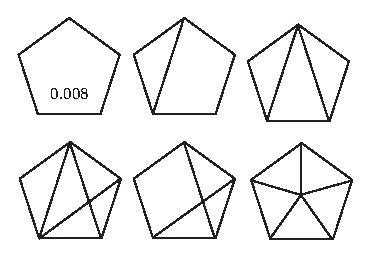
\includegraphics{PS/penthex.eps}
  \caption{Pentagonal Face Refinements}
  \label{fig:penthex}
\end{figure}

\begin{figure}[htb]
  \centering
  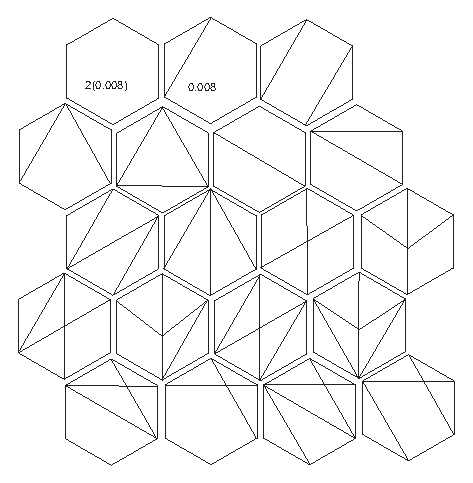
\includegraphics{PS/hexrefine_xxx.eps}
  \caption{Hexagonal Face Refinements.
    The only figures with a penalty are the first two on the top
    row and those on the bottom row.  The first two on the top row
    have penalties $2(0.008)$ and $0.008$.  Those on the bottom
    row have penalties $3\xiG$, $3\xiG$, $\xiG+2\xiV$, and
    $\xiG+2\xiV$.
  }
  \label{fig:hexrefine}
\end{figure}

The conventions for generating the possibilities are different for
the pentagons and hexagons than for the heptagons and octagons. We
describe the pentagons and hexagons first.  We erase all
$3$-unconfined upright diagonals. If there is one loop we leave
the loop in the figure. If there are two loops (so that both
necessarily have context $(n,k)=(4,1)$), we erase one and keep the
other.

The figures are interpreted as follows.  An internal vertex in the
polygon represents an upright diagonal.  Edges from that vertex are
in $1$-$1$ correspondence with the anchors around that upright
diagonal.  Edges between nonadjacent vertices of the polygon
represent the diagonals of flat quarters.  We draw all edges from an
upright diagonal to its anchors, and all edges of length
$[2t_0,2\sqrt2]$ that are not masked by upright quarters. Since the
only remaining upright quarters belong to loops, the four simplices
around a loop are anchored simplices and the edge opposite the
diagonal has length at most $3.2$.

Various inequalities in the inequality archive have been designed
for subregions of pentagons. Additional inequalities have been
designed for subregions in hexagonal regions.  Thus, we are able
to obtain greatly improved linear programming bounds when we break
each pentagonal region into various cases, according to the list
of Figures~\ref{fig:penthex} and \ref{fig:hexrefine}.

\section{Hept and Oct Branching}

When the figure is a heptagon or octagon, we proceed differently.
We erase all $3$-unconfined upright diagonals and all loops
(either context $(n,k)=(4,1)$ or $(4,2)$) and draw only  the flat
quarters.  An undrawn diagonal of the polygon has length at least
$2t_0$.  Overall, in these cases much less internal structure is
represented.

\begin{figure}[htb]
  \centering
  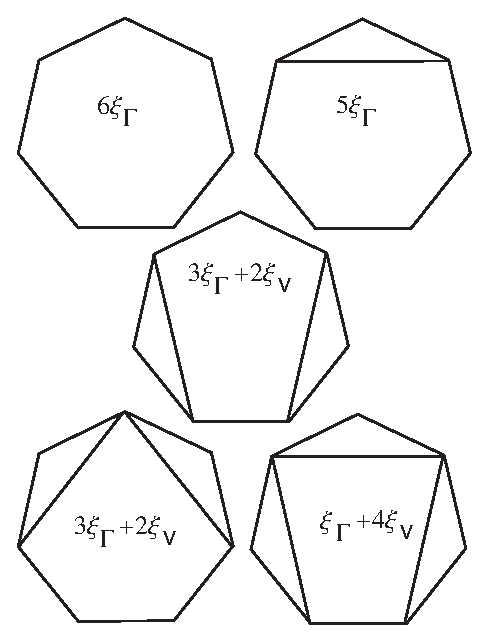
\includegraphics{PS/heptrefine.eps}
  \caption{Hept Face Refinements}
  \label{fig:heprefine}
\end{figure}

\begin{figure}[htb]
  \centering
  \includegraphics{PS/octrefine.eps}
  \caption{Oct Face Refinements}
  \label{fig:octrefine}
\end{figure}

In the cases where $3$-confined upright diagonals or loops have
been erased, a number indicating a penalty accompanies the
diagram. These penalties are derived in \shortversion{\cite{KC}.}
\longversion{Sections~\ref{sec:penalty} and \ref{sec:penalty1}.}

Define values
    $$
    Z(3,1)=0.00005\quad\text{and }D(3,1)=0.06585.
    $$

Here are some special arguments that are used for heptagons and
octagons.

\subsection{One flat quarter}
Suppose that the standard region breaks into two
subregions: the triangular region of a flat quarter $Q$ and one
other. Let $n=n(R)\in\{7,8\}$. We have the inequality:
    $$
    \sigma_R(D) < (\hat\sigma(Q)-Z(3,1)) + s_{n} +\xiG+2\xiV.
    $$
The penalty term $\xiG+2\xiV$ comes from a possible anchored
simplex masking a flat quarter.   Let $v$ be the central vertex of
the flat quarter $Q$.  Let $\{v_1,v_2\}$ be its diagonal. Masked
flat quarters satisfy restrictive edge constraints.  It follows
from \shortversion{\cite{KC}}
\longversion{Section~\ref{sec:some-flat}} that we have one of the
following three possibilities:
    \begin{enumerate}
    \item $y[v] \ge 2.2$,
    \item $e[v_1,v_2] \ge2.7$,
    \item $\sigma_R(D) < (\hat\sigma(Q)-Z(3,1)) + s_{n(R)}.$
    \end{enumerate}

\subsection{Two flat quarters}
We proceed similarly if the standard region $R$ breaks
into three subregions: two regions $R_1$ and $R_2$ cut out by flat
quarters $Q_1$, $Q_2$ and one other region made from what remains.
Write $\hat\sigma_1$ for $\hat\sigma(Q_1)$, and so forth.  It
follows from \shortversion{\cite{KC}}
\longversion{Section~\ref{sec:some-flat}} that we have one of the
following three possibilities:
    \begin{enumerate}
    \item The height of a central vertex is at least $2.2$.
    \item The diagonal of a flat quarter is at least $2.7$.
    \item
        $$
        \begin{array}{lll}
        \sigma_R(D) &< (\hat\sigma_1-Z(3,1)) +
            (\hat\sigma_2-Z(3,1))+ s_{n(R)},\\
        \tau_R(D)
        &>(\hat\tau_1-D(3,1))+(\hat\tau_2-D(3,1))+t_{n(R)}.
        \end{array}
        $$
    \end{enumerate}


With heptagons, it is helpful on occasion to use an upper bound on the
penalty of $3\xiG = 0.04683$. This bound holds if neither flat quarter
is masked by a loop. For this, it suffices to show that first two of the
given three cases do not hold.

%\subsubsection{Octagon Branching}.

If there is a loop of context $(n,k)=(4,2)$, we have the upper
bounds of Lemma~\ref{lemma:loop:bis}.  If, on the other hand,
there is no loop of context $(n,k)=(4,2)$, then we have the upper
bound
    $$
    \sigma_R(D)\le
    (\hat\sigma(Q_1)-Z(3,1)) +
    (\hat\sigma(Q_2)-Z(3,1)) + s_{n(R)} + 2(\xiG+2\xiV),
    $$
where $n(R)\in\{7,8\}$.


\section{Branching on Upright Diagonals} %subsection
\label{sec:4.12}

We divide the upright simplices into two domains depending on the
height of the upright diagonal, using $|v|=2.696$ as the dividing
point. We break the upright diagonals (of unerased quarters in the
$Q$-system) into cases:
    \begin{enumerate}
    \item The upright diagonal has height at most $2.696$.
    \item The upright diagonal $\{0,v\}$ has height at least $2.696$,
        and some anchor $w$ along the flat quarter satisfies
        $|w|\ge 2.45$ or $|v-w|\ge2.45$.  (There is a separate
        case here for each anchor $w$.)
    \item The upright diagonal $\{0,v\}$ has height at least
    $2.696$,
        and every anchor $w$ along the flat quarter satisfies
        $|w|\le 2.45$ and $|v-w|\le2.45$.
    \end{enumerate}
Many inequalities have been specially designed to hold on these smaller
domains.  They are included into the linear programming problems as
appropriate.

When all the upright quarters can be erased, then the case for
upright quarters follows from some other case without the upright
quarters.  An upright quarter can be erased in the following
situations.  If the upright quarter $Q$ has compression type (in
the sense of Definition~\ref{def:sigma}) and the diagonal has
height at least $2.696$,
then\footnote{\calc{214637273}. %Here $\sigma=\nu_\Gamma$.
}
    $$\sigma(Q)<\svor_0(Q)$$
%(Calculations~\ref{x-calc:AA10}).
(If there are masked flat quarters, they become scored by
$\hat\sigma$.) If an upright quarter has Voronoi type and the
anchors $w$ satisfy $|w|\le 2.45$ and $|v-w|\le2.45$, then the
quarter can be erased\footnote{\calc{378432183}.  %Here $\sigma=\nu$.
}
    $$\sigma(Q)<\svor_0(Q)$$
In general, we only have the weaker
inequality\footnote{\calc{310679005}.  %Here $\sigma=\nu$.
}
%(Inequality~\ref{x-calc:AA11})
    $$\sigma(Q)< \svor_0(Q)+0.003521.$$


%\section{Branching on Upright Quarters} %section
%\label{sec:6}

In a pentagon or hexagon, consider an upright diagonal with three
upright quarters, that is, context $(n,k)=(4,1)$. If the upright
diagonal has height at most $2.696$, and if an upright quarter
shares both faces along the upright diagonal with other upright
quarters, then we may assume that the upright quarter has
compression type. For otherwise, there is a face of circumradius
at least $\sqrt2$, and
hence two upright quarters of Voronoi type.  The inequality % where is this?
    \begin{equation} \octavor <
    \octavor_0 - 0.008,
    \label{eqn:6.1}
    \end{equation}
if $y_1\in[2t_0,2.696]$, and $\eta_{126}\ge\sqrt2$ shows that the
upright quarters can be erased without penalty because
    $$\xiG -0.008-0.008 <0.$$
If erased, the case is treated as part of a different case.

This allows the inequalities\footnote{See, for example,
\calc{867513567-*}} to be used that relate specifically to upright
quarters of compression type.
% Appendix \ref{app:nugamma1} and \ref{app:nugamma}
Furthermore, it can often be concluded that all three upright
quarters have compression type. For this, we use various
inequalities in the archive
    %%\ref{app:471} and \ref{app:455}}
which can often be used to show that if the anchored simplex has a
face of circumradius at least $\sqrt2$, then the linear
programming bound on $\sigma(D)$ is less than $8\,\pt$.



\section{Branching on Flat Quarters}

We make a few general remarks about flat quarters.



\begin{remark}
Information about the internal structure of an exceptional face
gives improvements to the constants $1.4\,\pt$ and $1.5\,\pt$ of
Property \ref{definition:admissible:excess} in the definition of
admissible weight assignments. (The bounds remain fixed at
$1.4\,\pt$ and $1.5\,\pt$, but these arguments allow us to specify
more precisely which simplices contribute to these bounds.) These
constants contribute to the bound on $\tau(D)$ through the
admissible weight assignment. Assume that at the vertex $v$ there
are four quasi-regular tetrahedra and an exceptional face, and
that the exceptional face has a flat quarter with central vertex
$v$. The calculations of Section \ref{sec:tri34} show that the
union $F$ of the four quasi-regular tetrahedra and exceptional
region give $\tau_F(D)\ge 1.5\,\pt$. If there is no flat quarter
with central vertex $v$, then the union $F$ of four quasi-regular
tetrahedra along $\{0,v\}$ give $\tau_F(D)\ge 1.5\,\pt$. We can make
similar improvements when $tri(v)=3$.
\end{remark}

\begin{remark} There are a few  other interval-based inequalities that are
used in particular cases. The inequalities
    $y_1\le 2.2, y_4\le2.7, \eta_{234},\eta_{456}\le\sqrt2$
imply that the flat quarter has compression type (see
Section~\ref{sec:rules}). The circumradius is not a
linear-programming variable, so its upper bound must be deduced
from edge-length information.
\end{remark}

If all three corners of a flat quarter have height at most 2.14,
and if the diagonal has length less than $2.77$, then the
circumradius of the face containing the origin and diagonal is at
most $\eta(2.14,2.14,2.77)<\sqrt2$.  This allows us to branch
combine into three cases.
\begin{lemma}
    Let $Q$ be a flat quarter whose corners $v_i$ have height at most $2.14$ and
    whose diagonal is at most $2.77$.  Then one of the following is true.
        \begin{enumerate}
    \item $\sigma(Q)=\Gamma(Q)$.
    \item The diagonal has length $\le2.7$, $\eta(y_4,y_5,y_6)\ge\sqrt2$,
        and $\sigma(Q)\le \svor_0(Q)$.
    \item The diagonal has length $\ge2.7$ and $\sigma(Q)\le\svor_0(Q)$.
    \end{enumerate}
\end{lemma}

\begin{proof} Case 1 holds when $Q$ is a quarter of compression
type in the $Q$-system.  If $Q$ is in the $Q$-system but is not of
compression type, then $\eta(y_4,y_5,y_6)\ge\sqrt2$ and
$\sigma(Q)\le \svor_0(Q)$.  If $Q$ is not in the $Q$-system, then
$\svor_0(Q)$ is an upper bound \shortversion{\cite{KC}.}
\longversion{Lemma~\ref{lemma:hatsigma}.} If $Q$ is not in the
$Q$-system, then its diagonal has length at least $2.7$, or the
central vertex has height at most $2.2$ (see
Lemma~\ref{lemma:2.7}.) In this case, we use the upper bound
$\svor_0(Q)$.
\end{proof}

Various inequalities in the archive have designed specifically for
each of these three cases.  Thus, whenever the hypotheses of the
lemma are met, we are able to improve on the linear programming
bounds by breaking into these three cases.
%We use the specially tailored Inequalities \ref {app:A.7.1} and
%\ref {app:A.7.2}.

\section{Branching on Simplices that are not Quarters}

\begin{lemma}
Suppose that  a triangular subregion comes from a simplex $S$ with
one vertex at the origin and three other vertices of height at
most $2t_0$.  Suppose that the edge lengths of the fourth, fifth,
and sixth edges satisfy $y_5,y_6\in[2t_0,2\sqrt2]$,
$y_4\in[2,2t_0]$. Suppose that $\min(y_5,y_6)\le2.77$. Then one of
the following is true.
    \begin{enumerate}
    \item  The edges have lengths $y_5,y_6\in[2t_0,2.77]$,
    $\eta_{456}\ge\sqrt2$, and $\sigma(S) \le \svor_0(S)$.
    \item
    $y_5,y_6\in[2t_0,2.77]$, and $\sigma(S) \le \svor(S)$
     (the analytic Voronoi function).
    \item An edge (say $y_6$)
    has length $y_6\ge2.77$ and $\sigma(S) \le \svor_0(S)$.
    \end{enumerate}
\end{lemma}

\begin{proof} If we ignore the statements about $\sigma$, then the
conditions in the Lemma concerning edge-length are exhaustive.
The bounds on $\sigma$ in each case are given by
\shortversion{\cite{KC}.}
\longversion{Section~\ref{sec:separation}.}
\end{proof}

There are linear programming inequalities that are tailored to
each case.

%We use the specially tailored Inequalities \ref{app:17}.

%If there is an enclosed vertex of height at most $\sqrt2$, then we can
%use Inequalities \ref{app:A.7.4}.


\longversion{\section{Branching on Quadrilateral subregions}}

\longversion{One of the inequalities of
%\ref{app:471}
holds for a quadrilateral subregion, if certain conditions are
satisfied.  One of the conditions is $y_4\in[2\sqrt2,3.0]$, where
$y_4$ is a diagonal of the subregion. Since this diagonal is not
one of the linear programming variables, these bounds cannot be
verified directly from the linear program.  Instead we use an
inequality
%\ref{ineq:1.678}
which relates the desired bound $y_4\le3$ to the linear
programming variables $\alpha[v,F]$, $y_2$, $y_3$, $y_5$, and
$y_6$.}

    % Implementation Details...

\section{Implementation Details for Branching}
\label{sec:facerefinement}

We will now make a detailed examination of the internal structure
of exceptional regions.

A {\it refinement\/} $\tildeF$ of a face $F$ of a plane graph $G$
is a set $\tildeF$ of faces  such that
    \begin{enumerate}
    \item The intersection of
the vertex set of $G$ with that of $\tildeF$ is the set $F$.
    \item $\tildeF \cup\{F^{op}\}$ is a plane graph.
    \end{enumerate}
We use refinements of faces to describe the internal structure of
faces.

We introduce indexing sets $\marku{FACE-\tildeF }$,
$\marku{VERTEX-\tildeF }$, $\marku{ANGLE-\tildeF }$,
$\marku{EDGE-\tildeF }$, the sets of faces, vertices, angles, and
edges in $\tildeF$, respectively, analogous to those introduced
for $G$.

We create variables
    $\pi[\tildeF]$, and indexed variables
    $$
    \begin{array}{lll}
    \sol\{\marku{FACE-\tildeF }\}, & \sc\{\marku{FACE-\tildeF }\} &
    \tausc\{\marku{FACE-\tildeF }\},\\
    \alpha\{\marku{ANGLE-\tildeF }\}, & y\{\marku{VERTEX-\tildeF }\}, &
    e\{\marku{EDGE-\tildeF }\}.
    \end{array}
    $$
(Variables with names ``$y[v]$'' and ``$e[v,w]$'' were already
created for some $v,w\in \marku{VERTEX-\tildeF }\cap
\marku{VERTEX}$.  In these cases, we use the variables already
created.)

Each vertex $v$ in the refinement will be interpreted either as a
vertex $v^I\in U(D)$, or as the endpoint of an upright diagonal
lying over the standard region $F^I$. We will interpret the faces
of the refinement in terms of the geometry of the decomposition
star $D$ variously as flat quarters, upright quarters, anchored
simplices, and the other constructs of \Part~\ref{part:bounds}.
This interpretation depends on the context, and will be described
in greater detail below.

Once the interpretation of faces is fixed, the interpretations are
as before for the variable names introduced already: $y$, $e$,
$\alpha$, $\sol$.  The lower and upper bounds for $\alpha$ and
$\sol$ are as before.  The lower and upper bounds for $y[v]$ are
$2$ and $2t_0$ if $v^I\in U(D)$, but if $(0,v^I)$ is an upright
diagonal, then the bounds are $[2t_0,2\sqrt2]$. The lower and
upper bounds for $e$ will depend on the context.

\section{Variables related to score}
\label{sec:variable}

The variables $\sc$ are a stand-in for the score $\sigma$ on a
face. We do not call them $\sigma$ because the sum of these
variables will not in general equal the variable $\sigma[F]$, when
$\tildeF$ is a refinement of $F$:
    $$[\sum_{F'\in \tildeF }\sc[F'] \ne \sigma[F]].$$
We will use have a weaker relation:
    $$\sigma[F] \le \sum_{F'\in \tildeF }\sc[F'] + \pi[\tildeF].$$
The variable $\pi[\tildeF]$ is called the penalty associated with
the refinement $\tildeF$.  (Penalties are discussed at length in
\shortversion{\cite{KC}.} \longversion{Sections \ref{sec:penalty}
and \ref{sec:penalty1}.}) The interpretations of $\sc$ and
$\pi[\tildeF]$ are rather involved, and will be discussed on a
case-by-case basis below. The interpretation of $\tausc$ follows
from the identity:
    $$\tausc[F'] = \sol[F']\zeta\pt - \sc[F'],\quad\forall
    F'\in \tildeF .$$

The interpretation of variables that follows might appear to be
hodge-podge at first.  However, they are obtained in a systematic
way. We analyze the proofs and approximations in
Part~\ref{part:bounds}, and define $\sc[F]^I$ as the best
penalty-free scoring approximation that is consistent with the
given face refinement. here are the details.

If the subregion is a flat quarter, the interpretation of $\sc[F]$
is the function $\hat\sigma$, defined in \shortversion{\cite{KC}.}
\longversion{\ref{sec:some-flat}.}  If the subregion is an upright
quarter $Q$, the interpretation of $\sc[F]$ is the function
$\sigma(Q)$ from Section~\ref{sec:scoring}. If the subregion is an
anchored simplex that is not an upright quarter, $\sc[F]$ is
interpreted as the analytic Voronoi function $\vor$ if the simplex
has type $C$ or $C'$, and as $\vor_0$ otherwise. (The types $A$,
$B$, $C$ and $C'$ are defined in Section~\ref{x-2.5}.) Whether or
not the simplex has type $C$, the inequality $\sc[F]\le0$ is
satisfied. In fact, if $\vor_0$ scoring is used, we note that
there are no quoins, and $\phi(1,t_0)<0$.

If the subregion is triangular, if no vertex represents an upright
diagonal, and if the subregion is not a quarter, then $\sc[F]$ is
interpreted as  $\vor$ or $\vor_0$ depending on whether the
simplex has type $A$.  In either case, the inequality
$\sc[F]\le\vor_0$ is satisfied.

In most other cases, the interpretation of $\sc[F]$ is $\vor_0$.
However, if $R$ is a heptagon or octagon, and $F$ has $\ge4$
sides, then $\sc[F]$ is interpreted as $\vor_0$ except on
simplices of type $A$, where it becomes the analytic Voronoi
function.

If $R$ is a pentagon or hexagon, and $F$ is a quadrilateral that is
not adjacent to a flat quarter, and if there are no penalties in the
region, then the interpretation of $\sc[F]$ is the actual score of
the subregion over the subregion. In this case, the score $\sigma_R$
has a well-defined meaning for the quadrilateral, because it is not
possible for an upright quarter in the $Q$-system to straddle the
quadrilateral region and an adjacent region. Consequently, any
erasing that is done can be associated with the subregion without
ambiguity. By the results of \Chaps~\ref{sec:break_piece}
and~\ref{sec:proofs}, we have $\sc[F]\le0$. We also have
$\sc[F]\le\vor_0$.

One other bound that we have not explicitly mentioned is the bound
$\sigma_R(D)< s_n$.  For heptagons and octagons that are not
aggregates, this is a better bound than the one used in the
definition of tameness (Property~\ref{definition:tame:score}). In
heptagons and octagons that are not aggregates, if we have a
subregion with four or more sides, then $\sc[F]< Z(n,k)$ and
$\tausc[F]>D(n,k)$. (See Section~\ref{x-5.5},
Equations~\ref{eqn:tau>D(n,k)} and \ref{eqn:sigma<Z(n,k)}.


The variables are subject to a number of compatibility relations
that are evident from the underlying definitions and geometry.
    $$
    \begin{array}{lll}
    \sol[F'] = \sum_{v\in F'}\alpha[v,F'] - (len[F']-2)\pi,&\forall F'\\
    \sum_{F':v\in F',F'\in \marku{FACE-\tildeF }} \alpha[v,F'] =
    \alpha[v,F], &\forall v
    \end{array}
    $$

Assume that a face $F_1\in \tildeF$ has been interpreted as a
subregion $R=F_1^I$ of a standard region.  Assume that each vertex
of $F_1$ is interpreted as a vertex in $U(D)$ or as the endpoint
of an upright diagonal over $F^I$.  One common interpretation of
$\sc$ is $\vor_{0,F}(U(D))$, the truncated Voronoi function. When
this is the interpretation, we introduce further variables:
    $$
    \begin{array}{lll}
    \quo[v,s(v,F_1)] & \forall v\in F_1,\\
    \quo[s(v,F_1),v] & \forall v\in F_1,\\
    \Adih[v,F_1] & \forall v\in F_1,\\
    \end{array}
    $$
We interpret the variables as follows. If $w = s(v)$, and the
triangle $(0,v^I,w^I)$ has circumradius $\eta$ at most $t_0$, then
    $$
    \begin{array}{lll}
    \quo[v,w]^I &= \quo(R(|v^I|/2,\eta,t_0)),\\
    \quo[w,v]^I &= \quo(R(|w^I|/2,\eta,t_0)).
    \end{array}
    $$
If the circumradius is greater than $t_0$, we take
    $$\quo[v,w]^I =\quo[w,v]^I =0.$$
The variable $\Adih$ has the following interpretation:
    $$\Adih[v,F_1]^I = \begin{cases}
        A(|v^I|/2)\alpha(v^I,F_1^I) & |v^I|\le 2t_0,\\
        0 & \text{otherwise.}\\
        \end{cases}
    $$
Under these interpretations, the following identity is satisfied:
    $$
    \begin{array}{lll}
    \sc[F_1] &= \sol[F_1]\phi_0 +\sum_{v\in F_1} \Adih[v,F_1]\\
            &\quad - 4\doct \sum \quo[v,w].
    \end{array}
    $$
%This relation and the constants that appear in it are based on
%Calculations~\ref{calc:quo}.
The final sum runs over all pairs
$(v,w)$, where $v=s(w,F_1)$ or $w=s(v,F_1)$.

For this to be useful, we need good inequalities governing the
individual variables.  Such inequalities for $\Adih[v,F]$ and
$\quo[v,w]$ are found in Calculations~\calc{815275408} and
\calc{349475742}. To make of use these inequalities, it is
necessary to have lower and upper bounds on $\alpha[v,F]$ and
$y[v]$.  We obtain such bounds as LP-derived inequalities in the
sense of Remark \ref{remark:derived}.


\section{Appendix Hexagonal Inequalities}

There are a number of inequalities that have been particularly
designed for standard regions that are hexagons.  This appendix
describes those inequalities.  They are generally inequalities
involving more than six variables, and because of current
technological limitations on interval arithmetic, we were not able
to prove these inequalities directly with interval arithmetic.

Instead we give various lemmas that deduce the inequalities from
inequalities in a smaller number of variables (small enough to
prove by interval arithmetic.)


\subsection{Statement of results} %\endsubhead



There are a number of inequalities that hold in special situations
when there is a hexagonal region.  Although these inequalities do
not appear in the main text of the proof of the Kepler conjecture,
they are used in the linear programs.

After stating all of them, we will turn to the proofs.

\begin{enumerate}
\item\label{app:hex1}
 If there are no flat quarters and no upright quarters (so that
there is a single subregion $F$), then
    \begin{eqnarray}%{lll}
    \vor_0 &< -0.212\\
    \tau_0 &> 0.54525.
    \end{eqnarray}
    %\label{eqn:4.6.1}
    \oldlabel{eqn:4.6.1}

\item \label{app:hex2} If there is one flat quarter and no upright
quarters, there is a pentagonal subregion $F$.  It satisfies
    $$
    \begin{array}{lll}
    \vor_0 &< -0.221\\
    \tau_0 &> 0.486.
    \end{array}
    %\label{eqn:4.6.2}
    $$

\item\label{app:hex3} If there are two flat quarters and no
upright quarters, there is a quadrilateral subregion $F$.  It
satisfies
    $$
    \begin{array}{lll}
    \vor_0 &< -0.168,\\
    \tau_0 &> 0.352.
    \end{array}
    %\label{eqn:4.6.3}
    $$
These are twice the constants appearing in \ref{app:hex11};


\item\label{app:hex4} If there is an edge of length between $2t_0$
and $2\sqrt2$ running between two opposite corners of the
hexagonal cluster, and if there are no flat or upright quarters on
one side, leaving a quadrilateral region $F$, then $F$ satisfies
    $$
    \begin{array}{lll}
    \vor_0 &< -0.075,\\
    \tau_0 &> 0.176.
    \end{array}
    %\oldlabel{eqn:4.6.4}
    $$

\item\label{app:hex5} If the hexagonal cluster has an upright
diagonal with context $(4,2)$, and if there are no flat quarters
(Figure~\ref{fig:hex42}), then the hexagonal cluster $R$ satisfies
    $$
    \begin{array}{lll}
    \sigma_R &< -0.297,\\
    \tau_R &> 0.504.
    \end{array}
    %\oldlabel{eqn:4.6.5}
    $$
\begin{figure}[htb]
  \centering
  \includegraphics{PS/hex42.eps}
  \caption{A hexagonal cluster with context $(4,2)$.}
  \label{fig:hex42}
\end{figure}

\item\label{app:hex6} If the hexagonal cluster has an upright
diagonal with context $(4,2)$, and if there is one unmasked flat
quarter (Figure~\ref{fig:hex42a}, let $\{F\}$ be the set of four
subregions around the upright diagonal. (That is, take all
subregions except for the flat quarter.) In the following
inequality and Inequality \ref{app:hex7}, let $\sigma_R^+$ be
defined as $\sigma_R$ on quarters, and $\vor_x$ on other anchored
simplices.  $\tau_R^+$ is the adapted squander function.
    $$
    \begin{array}{lll}
    \sum_{(4)}\sigma_R^+ &< -0.253,\\
    \sum_{(4)}\tau_R^+ &> 0.4686.\\
    \end{array}
    %\oldlabel{eqn:4.6.6}
    $$
\begin{figure}[htb]
  \centering
  \includegraphics{PS/hex42a.eps}
  \caption{A hexagonal cluster with context $(4,2)$.}
  \label{fig:hex42a}
\end{figure}


\item\label{app:hex7} If the hexagonal cluster has an upright
diagonal with context $(4,2)$, and if there are two unmasked flat
quarters (Figure~\ref{fig:hex42b}), let $\{F\}$ be the set of four
subregions around the upright diagonal. (That is, take all
subregions except for the flat quarters.)
    $$
    \begin{array}{lll}
    \sum_{(4)}\sigma_R^+ &< -0.2,\\
    \sum_{(4)}\tau_R^+ &> 0.3992.\\
    \end{array}
    %\oldlabel{eqn:4.6.7}
    $$
\begin{figure}[htb]
  \centering
  \includegraphics{PS/hex42b.eps}
  \caption{A hexagonal cluster with context $(4,2)$.}
  \label{fig:hex42b}
\end{figure}

\item\label{app:hex8} If the hexagonal cluster has an upright
diagonal in context $(4,1)$, and if there are no flat quarters,
let $\{F\}$ be the set of four subregions around the upright
diagonal. Assume that the edge opposite the upright diagonal on
the anchored simplex has length at least $2\sqrt2$.
 (See Figure~\ref{fig:hex41}.)
    $$
    \begin{array}{lll}
    \vor_{0,R}(D)+\sum_{(3)}\sigma(Q) &< -0.2187\\
    \tau_{0,R}(D)+\sum_{(3)}\tau(Q) &> 0.518.
    \end{array}
    %\oldlabel{eqn:4.6.8}
    $$
\begin{figure}[htb]
  \centering
  \includegraphics{PS/hex41.eps}
  \caption{A hexagonal cluster with context $(4,1)$.}
  \label{fig:hex41}
\end{figure}

\item\label{app:hex9} In this same context, let $F$ be the
pentagonal subregion along the upright diagonal. It satisfies
    \begin{eqnarray}
    \vor_0 &< -0.137,\\
    \tau_0 &> 0.31.
    \end{eqnarray}
    %\oldlabel{eqn:4.6.9}

\item\label{app:hex10} If the hexagonal cluster has an upright
diagonal in context $(4,1)$, and if there is one unmasked flat
quarter, let $\{F\}$ be the set of four subregions around the
upright diagonal. Assume that the edge opposite the upright
diagonal on the anchored simplex has length at least $2\sqrt2$.
 (There are five subregions, shown in Figure~\ref{fig:hex41a}.)
    $$
    \begin{array}{lll}
    \vor_{0,R}(D)+\sum_{(3)}\sigma(Q) &< -0.1657,\\
    \tau_{0,R}(D)+\sum_{(3)}\tau(Q) &> 0.384.
    \end{array}
    %\oldlabel{eqn:4.6.10}
    $$
\begin{figure}[htb]
  \centering
  \includegraphics{PS/hex41a.eps}
  \caption{A hexagonal cluster with context $(4,1)$.}
  \label{fig:hex41a}
\end{figure}

\item\label{app:hex11} In this same context, let $F$ be the
quadrilateral subregion in Figure~\ref{fig:hex41a}. It satisfies
    $$
    \begin{array}{lll}
    \vor_0 &< -0.084,\\
    \tau_0 &> 0.176.
    \end{array}
    %\oldlabel{eqn:4.6.11}
    $$


\end{enumerate}


\subsection{Proof of inequalities}
\label{app:hexquad}


\begin{proposition}  Inequalities \ref{app:hex1} --\ref{app:hex11}  are valid.
\end{proposition}

 We prove the inequalities in reverse order \ref{app:hex11}--
\ref{app:hex1}. The bounds\footnote{\calc{148776243}} %2002_IV_A13
   $\vor_0<0.009$ and $\tau_0>0.05925$
%from [$\A_{13}$]
for what a flat quarters with diagonal $\sqrt8$  will be used
repeatedly.  Some of the proofs will make use of tcc-bounds, which
are described in \ref{x-4.10}.
% [Section~5.2]

\begin{proof}
({\it Inequality \ref{app:hex10} and Inequality \ref{app:hex11}.})
Break the quadrilateral cluster into two simplices $S$ and $S'$
along the long edge of the anchored simplex $S$.  The anchored
simplex $S$ satisfies $\tau(S)\ge0$, $\sigma(S)\le0$.  The other
simplex satisfies $\tau_0(S')>0.176$ and $\vor_0(S')<-0.084$ by an
interval calculation.\footnote{\calc{938091791}} % (* kc group 18.16 : app:p11 *)
%\footnote{\calc{}} \ref{app:p11}..
  This gives Inequality \ref{app:hex11}.  For Inequality
\ref{app:hex10}, we combine these bounds with the linear
programming bound on the four anchored simplices around the
upright diagonal.  From a series of
inequalities%
\footnote{\calc{815492935}, \calc{187932932}, \calc{485049042},
\calc{835344007}}
%    [$\A_2$]{part} --
%    [$\A_{7}$]{part},
%    [$\A_{22}$]{part},
%    [$\A_{24}$]{part},
we find that they score $<-0.0817$ and squander $>0.208$.  Adding
these to the bounds from Inequality \ref{app:hex11}, we obtain
Inequality \ref{app:hex10}.
\end{proof}

\begin{proof}
{\it (Inequality (\ref{app:hex8}) and (\ref{app:hex9}).)} The
pentagon is a union of an anchored simplex and a quadrilateral
region. LP-bounds similar to those in the previous paragraph and
based on the inequalities of Section~\ref{sec:loops} show that the
loop scores at most $-0.0817$ and squanders at least $0.208$.  If we
show that the quadrilateral satisfies
    \begin{eqnarray}
    \vor_0&<-0.137,\label{eqn:hexquadsig}\\
    \tau_0&>0.31,\label{eqn:hexquadtau}
    \end{eqnarray}
then Inequalities (\ref{app:hex8}) and (\ref{app:hex9}) follow. If
by deformations a diagonal of the quadrilateral drops to
$2\sqrt2$, then the result follows
 %from Inequalities \ref{app:p8} and
interval calculations.\footnote{\calc{148776243},\calc{468742136}} % (* kc group 18.15 : app:p8 *)
 %[$\A_{13}$]{part-4}.
 By this we may now assume that the
quadrilateral has the form
    $$(a_1,2,a_2,2,a_3,2,a_4,b_4),\quad a_2,a_3\in\{2,2t_0\}.$$
If the diagonals drop under $3.2$ and $\max(a_2,a_3)=2t_0$, again
the result follows from
 %Inequalities \ref{app:p8} and
 interval
calculations.\footnote{calc{148776243},\calc{468742136}} % (* kc group 18.15 : app:p8 *)
%[$\A_{13}$]{part-4}.
If the diagonals drop under $3.2$ and $a_2=a_3=2$, then the result
follows from further interval
calculations.\footnote{\calc{128523606}} %[$\A_{19}$]{part-4}.
So finally we attain by deformations $b_4=2\sqrt2$ with both
diagonals greater than $3.2$. But this does not exist, because
    $$\Delta(4,4,4,3.2^2,4,8,3.2^2)<0.$$
\end{proof}


\begin{proof}
{\it (Inequality \ref{app:hex5}, Inequality \ref{app:hex6}, and
Inequality \ref{app:hex7}.)} Inequalities \ref{app:hex7} are
derived in Section~\ref{x-5.11}. Inequalities \ref{app:hex5},
\ref{app:hex6} are LP-bounds based on interval
calculations.\footnote{\calc{815492935}, \calc{187932932},
\calc{485049042}}
% [$\A_2$]{part-4}, [$\A_7$]{part-4}, [$\A_{22}$]{part-4}.
\end{proof}

\begin{proof} {\it (Inequality \ref{app:hex4}.)} Deform as in
Section~\ref{sec:BER}. If at any point a diagonal of the
quadrilateral drops to $2\sqrt2$, then the result follows from
interval
calculations\footnote{\calc{148776243}} % IVA13_ [$\A_{13}$]{part-4}
and Inequality \ref{app:hex11}:
    $$
    \begin{array}{lll}
    \vor_0 &< 0.009 -0.084 = -0.075,\\
    \tau_0 &> 0 + 0.176 = 0.176,\\
    \end{array}
    $$
Continue deformations until the quadrilateral has the form
    $$(a_1,2,a_2,2,a_3,2,a_4,b_4),\quad a_2,a_3\in\{2,2t_0\}.$$
There is necessarily a diagonal of length $\le3.2$, because
    $$\Delta(4,4,3.2^2,8,4,3.2^2)<0.$$
Suppose the diagonal between vertices $v_2$ and $v_4$ has length
at most $3.2$.  If $a_2=2t_0$ or $a_3=2t_0$, the result follows
from interval calculations\footnote{\calc{148776243}} % IVA13_ [$\A_{13}$]{part-4}
and Inequality \ref{app:hex11}. Take $a_2=a_3=2$. Inequality
\ref{app:hex4} now follows from interval
calculations.\footnote{\calc{128523606}} % IVA19_ [$\A_{19}$]{part-4}.
\end{proof}

\begin{proof}
{\it (Inequality \ref{app:hex3}).}
 We prove that the quadrilateral
satisfies
    $$
    \begin{array}{lll}
    \vor_0 &< -0.168\\
    \tau_0 &> 0.352.\\
    \end{array}
    $$
There are two types of quadrilaterals.  In (a), there are two flat
quarters whose central vertices are opposite corners of the
hexagon.  In (b), the flat quarters share a vertex.
  We consider case (a) first.

Case (a). We deform the quadrilateral as in
Section~\ref{sec:BER}.%{part-4}.
If at any point there is a
diagonal of length at most $3.2$, the result follows from
Inequality \ref{app:hex10} and Inequality \ref{app:hex11}.
Otherwise, the deformations give us a quadrilateral
    $$(a_1,2,a_2,2t_0,a_3,2,a_4,2), \quad a_i \in\{2,2t_0\}.$$
The tcc approximation now gives the result (see
\Chap~\ref{x-4.11}).
%[5.3)]{part-4}.

Case (b). Label the vertices of the quadrilateral
 $v_1,\ldots,v_4$, where $(v_1,v_2)$ and $(v_1,v_4)$
are the diagonals of the flat quarter.  Again, we deform the
quadrilateral.  If at any point of the deformation, we find that
$|v_1-v_3|\le 3.2$, the result follows from Inequalities
\ref{app:hex10}, \ref{app:hex11}. If during the deformation
$|v_2-v_4|\le2\sqrt2$, the result follows from
%[$\A_{13}$]{part-4}
interval calculations.\footnote{\calc{148776243},\calc{315678695}} % (* kc group 18.14 : app:p3  *)
 % IVA13_
 % \ref{app:p3}.
If the diagonal $(v_2,v_4)$ has length at least
$3.2$ throughout the deformation, we eventually obtain a
quadrilateral of the form
    $$(a_1,2t_0,a_2,2,a_3,2,a_4,2t_0),\quad a_i\in\{2,2t_0\}.$$
But this does not exist:
$$\Delta(4,4,3.2^2,(2t_0)^2,(2t_0)^2,3.2^2)<0.$$

We may assume that $|v_2-v_4|\in[2\sqrt2,3.2]$.  The result now
follows from interval calculations.\footnote{\calc{315678695}} % (* kc group 18.14 : app:p3  *)  \ref{app:p3}.
\end{proof}

\begin{proof}
{\it (Inequality \ref{app:hex2}).} This case requires more effort.
We show that
    $$
    \begin{array}{lll}
    \vor_0 &< -0.221\\
    \tau_0 &> 0.486\\
    \end{array}
    $$
Label the corners $(v_1,\ldots,v_5)$ cyclically with $(v_1,v_5)$ the
diagonal of the flat quarter in the hexagonal cluster. We use the
deformation theory of \Chap~\ref{sec:BER}.
%{part-4}.
The proof appears in
steps $(1),\ldots,(6)$.

(1) If during the deformations, $|v_1-v_4|\le3.2$ or
$|v_2-v_5|\le3.2$, the result follows from Inequalities
\ref{app:hexquad} and \ref{app:hex11}.  We may assume this does
not occur.

(2) If an edge $(v_1,v_3)$, $(v_2,v_4)$, or $(v_3,v_5)$ drops to
$2\sqrt2$, continue with deformations that do not further decrease
this diagonal. If $|v_1-v_3|=|v_3-v_5|=2\sqrt2$, then the result
follows from
    %[$\A_{13}$]{part-4}
interval calculations.\footnote{\calc{148776243},\calc{673399623}} % (* kc group 18.7 : app:p2a  *) % IVA13_
%\ref{app:p2a}.

If we have $|v_1-v_3|=2\sqrt2$, deform the figure to the form
    $$(a_1,2,a_2,2,a_3,2,a_4,2,a_5,2t_0),\quad a_2,a_4,a_5\in\{2,2t_0\}.$$
Once it is in this form, break the flat quarter $(0,v_1,v_2,v_3)$
from the cluster and deform $v_3$ until $a_3\in\{2,2t_0\}$.  The
result follows from an interval calculation.\footnote{\calc{297256991}} % (* kc group 18.8 : app:p2b *) \ref{app:p2b}.

We handle a boundary case of the preceding calculation separately.
After breaking the flat quarter off, we have the cluster
    $$(a_1,2\sqrt2,a_3,2,a_4,2,a_5,2t_0),\quad a_3,a_4,a_5\in\{2,2t_0\}.$$
If $|v_1-v_4|=3.2$, we break the quadrilateral cluster into two
pieces along this diagonal and use interval calculations\footnote{\calc{861511432}} % (* kc group 18.9 : app:p2c *)
%\ref{app:p2c}
to conclude the result. This completes the analysis
of the case $|v_1-v_3|=2\sqrt2$.

(3) If $|v_2-v_4|\le3.2$, then deform until the cluster has the
form
    $$(a_1,2,a_2,2,a_3,2,a_4,2,a_5,2t_0),\quad a_1,a_3,a_5\in\{2,2t_0\}.$$
Then cut along the special simplex to produce a quadrilateral.
Disregarding cases already treated by the interval calculations,\footnote{\calc{861511432}} % (* kc group 18.9 : app:p2c *)
%\ref{app:p2c},
we can deform it to
    $$(a_1,2,a_2,2\sqrt2,a_4,2,a_5,2t_0),\quad a_i\in\{2,2t_0\},$$
with diagonals at least $3.2$. The result now follows from
interval calculations.\footnote{\calc{746445726}} % (* kc group 18.10 : app:p2d *) \ref{app:p2d}.

In summary of (1), (2), (3), we find that by disregarding cases
already considered, we may deform the cluster into the form
    $$(a_1,2,a_2,2,a_3,2,a_4,2,a_5,2t_0),\quad a_i\in\{2,2t_0\},$$
$|v_1-v_3|>2\sqrt2$, $|v_3-v_5|>2\sqrt2$, $|v_2-v_4|>3.2.$

(4) Assume $|v_1-v_3|,|v_3-v_5|\le3.2$. If
$\max(a_1,a_3,a_5)=2t_0$, we invoke
 interval calculations\footnote{\calc{148776243},\calc{297256991}} % (* kc group 18.8 : app:p2b *) % IVA13_
%\ref{app:p2b}
%and [$\A_{13}$]{part-4}
to prove the
inequalities.
 So we may assume $a_1=a_3=a_5=2$.  The result now follows from
interval calculations.\footnote{\calc{897046482}} % (* kc group 18.11 : app:p2e *) \ref{app:p2e}.
This completes the case
$|v_1-v_3|,|v_3-v_5|\le3.2$.

(5) Assume $|v_1-v_3|,|v_3-v_5|\ge3.2$. We deform to
    $$(a_1,2,a_2,2,a_3,2,a_4,2,a_5,2t_0),\quad a_i\in\{2,2t_0\}.$$
If $a_2=2t_0$ and  $a_1=a_3=2$, then the simplex does not exist by
Section~\ref{x-5.6}.  %[5.6]{part-4}.
Similarly, $a_4=2t_0$, $a_5=a_3=2$ does not exist. The tcc bound
gives the result except when $a_2=a_4=2$. The condition
$|v_2-v_4|\ge3.2$ forces $a_3=2$. These remaining cases are
treated with interval calculations.\footnote{\calc{928952883}} % (* kc group 18.12 : app:p2f *) \ref{app:p2f}.

(6) Assume $|v_1-v_3|\le3.2$ and $|v_3-v_5|\ge3.2$. This case
follows from deformations, interval
calculations.\footnote{\calc{297256991},\calc{673800906}} % (* kc group 18.13 : app:p2g *) % (* kc group 18.8 : app:p2b *) \ref{app:p2b},
%and \ref{app:p2g}.
This completes the proof of Inequalities
\ref{app:hex2}.
\end{proof}

\smallskip
\begin{proof}
{\it (Inequality \ref{app:hex1}).} Label the corners of the hexagon
$v_1,\ldots,v_6$.  The proof to this inequality is similar to the
other cases.  We deform the cluster by the method of
\Chap~\ref{sec:BER} until it breaks into pieces that are small
enough to be estimated by interval calculations. If a diagonal
between opposite corners has length at most $3.2$, then the hexagon
breaks into two quadrilaterals and the result follows from
Inequality \ref{app:hexquad}.

If a flat quarter is formed during the course of deformation, then
the result follows from Inequality \ref{app:hex2} and interval
calculations.\footnote{\calc{148776243}} % IVA13_ [$\A_{13}$]{part-4}.
Deform until the hexagon
has the form
    $$(a_1,2,a_2,2,\ldots,a_6,2),\quad a_i\in\{2,2t_0\}.$$
We may also assume that the hexagon is convex (see
\Chap~\ref{x-4.13}). % [Section~4.11]{part-4}).

If there are no special simplices, we consider the tcc-bound. The
tcc-bound implies Inequality \ref {app:hex1}, except when $a_i=2$,
for all $i$. But if this occurs, the perimeter of the convex
spherical polygon is $6\arc(2,2,2)=2\pi$.  Thus, there is a pair
of antipodal points on the hexagon.  The hexagon degenerates to a
lune with vertices at the antipodal points.  This means that some
of the angles of the hexagon are $\pi$.   One of the tccs has the
form $C(2,1.6,\pi)$, in the notation of \Chap~\ref{x-4.11}.
%[Lemma~4.11]{part-4}.
With this extra bit of information, the
tcc bound implies Inequality \ref {app:hex1}.

If there is one special simplex, say $|v_5-v_1|\in[2\sqrt2,3.2]$,
we remove it. The score of the special simplex is\footnote{\calc{148776243}} % IVA13_
%[Inequalities $\A_{13}$]{part-4}
    $$
    \begin{array}{lll}
    \vor_0 &< 0,\quad \tau_0>0.05925,\quad\text{if }\max(|v_1|,|v_5|)=2t_0,\\
    \vor_0 &< 0.0461,\quad \tau_0>0,\quad\text{if }|v_1|=|v_5|=2,\\
    \end{array}
    $$
The resulting pentagon can be deformed. If by deformations, we
obtain $|v_2-v_5|=3.2$ or $|v_1-v_4|=3.2$, the result follows from
Inequalities \ref{app:hexquad} and two interval calculations.%
\footnote{\calc{725257062}, \calc{977272202}}

%\oldlabel{A.4.6.1.a}

%$\vor_0 < -0.212 -0.0461 +0.137$, if $y_4=3.2$,
%$y_5\in[2\sqrt2,3.2]$. \refno{725257062\dag}

%$\tau_0 > 0.54525 - 0 - 0.31$. if $y_4=3.2$,
%$y_5\in[2\sqrt2,3.2]$. \refno{977272202\dag}

If $|v_5-v_1|=2\sqrt2$, we use Inequality \ref{app:hex2} and
interval calculations\footnote{\calc{148776243}} % IVA13_ [$\A_{13}$]{part-4}
unless $|v_1|=|v_5|=2$. If $|v_1|=|v_5|=2$, we use  interval
calculations.\footnote{\calc{377409251}} % (* 18.3 : app:p1b *) \ref{app:p1b}.
If a second special simplex forms during the deformations, the
result follows from interval calculations.\footnote{\calc{586214007}} % (* 18.4 : app:p1c *) \ref{app:p1c}.

The final case of Inequality \ref{app:hex1}  to consider is that
of two special simplices. We divide this into two cases. (a) The
central vertices of the specials are $v_2$ and $v_6$.  (b) The
central vertices are opposite $v_1$ and $v_4$. In case (a), the
result follows by deformations and interval calculations.\footnote{\calc{89384104}} % (* 18.5 : app:p1d *)
%\ref{app:p1d}.
In case (b), the result follows by deformations and interval
calculations.\footnote{\calc{859726639}} % (* kc group 18.6 : app:p1e  *) \ref{app:p1e}.
This completes the proof of
Inequalities \ref{app:hex1} and the proof of the Proposition.
\end{proof}

    }

\shortversion{
    \label{part:tame}
    % Kepler Conjecture.
% Thomas C. Hales
% Starting with Chapter on Tame Hypermaps


%% XX Notation: A vs. v for nodes.
%% XX Notation sigma' for aggregates, sigma'' for the full hypermap.
%% Allow the pentagon-triangle into the definition of tame graph.
%%%% Show there is at most one.  Let it be the seed.
%%




\label{sec:tame}


This chapter defines a class of hypermaps.  Hypermaps in this class
are said to be {\it tame}.  In the next chapter, we give a complete
classification of all tame hypermaps.  This classification of tame
hypermaps was carried out by computer.   This classification is a
major step of the proof of the Kepler Conjecture.

\section{Definition and Classification}


\begin{definition}
Faces of cardinality $3$ are called {\it triangles}, those of
cardinality $4$ are called {\it quadrilaterals}, and so forth. Let
$p_v$ be the number of triangles incident with a node $v$. A face of
cardinality at least $5$ is called an {\it exceptional\/} face.
 %
 \index{triangle}
 \index{exceptional}
 \index{quadrilateral}
 \index{exceptional!face}
 \index{pZ@$p_v$}
\end{definition}

\begin{definition}\label{definition:type}
A face of a hypermap is said to be exceptional if it has at least
five darts.  The {\it type\/} of a node is defined to be a triple of
non-negative integers $(p,q,r)$, where $p$ is the number of
triangles containing the node, $q$ is the number of quadrilaterals
containing it, and $r$ is the number of exceptional faces.
%
 \index{type (of a node)}
\end{definition}


\subsection{weight assignment}\label{sec:wtassign}

We call the constant $\op{tgt}=14.8$, which arises repeatedly in
this section, the {\it target}.  (This constant arises as an
approximation to $4\pi\zeta -8\approx 14.7947$, where $\zeta =
1/(2\arctan(\sqrt{2}/5)$.)
%
 \index{target}\index{tgt@$\op{tgt}=14.8$}
 \index{ZZdzeta@$\zeta= 1/(2\arctan(\sqrt{2}/5))$}

\begin{definition}
  Define $a:\ring{N}\to \ring{R}$ by
  $$a(n) = \begin{cases}
    14.8 &n=0,1,2,\\
    1.4 & n=3,\\
    1.5 & n=4,\\
    0 & \text{otherwise.}
  \end{cases}
  $$
\end{definition}

\begin{definition}
  Define $b:\ring{N}\times \ring{N}\to \ring{R}$ by $b(p,q)=14.8$,
  except for the values in the following table
  (with  $\op{tgt}=14.8$):
  {
  \def\tx{\op{tgt}}
  $$\begin{matrix}  &q=0&1&2&3&4\\
           p=0&\tx&\tx&\tx&7.135&10.649\\
           1&\tx&\tx&6.95&7.135&\tx\\
           2&\tx&8.5&4.756&12.981&\tx\\
           3&\tx&3.642&8.334&\tx&\tx\\
           4&4.139&3.781&\tx&\tx&\tx\\
           5&0.55&11.22&\tx&\tx&\tx\\
           6&6.339&\tx&\tx&\tx&\tx
   \end{matrix}
   $$
   }
\end{definition}

\begin{definition}
  Define $c:\ring{N}\to \ring{R}$ by
  $$c(n) = \begin{cases}
    1 & n=3,\\
    0 & n=4,\\
    -1.03 &n=5,\\
    -2.06 &n=6,\\
    -3.03 &\text{otherwise.}
    \end{cases}
    $$
\end{definition}

\begin{definition}
    Define $d:\ring{N}\to \ring{R}$ by
  $$d(n) = \begin{cases}
    0 & n=3, \\
    2.378 & n=4, \\
    4.896 & n=5, \\
    7.414 & n=6, \\
    9.932 & n=7, \\
    10.916 & n=8,\\
    \op{tgt}=14.8 & \text{otherwise}.
  \end{cases}
  $$
\end{definition}

\begin{definition}
A set $V$ of nodes in a hypermap is called a {\it separated\/} set
of nodes if the following four conditions hold.
%
 \index{separated set}
    \begin{enumerate}
      \item Every node in $V$ is incident with an exceptional face.
      \item No two
        nodes in $V$ are adjacent.  (That is, no edge is incident
        with two different nodes in $V$.)
      \item No quadrilateral in $V$ is incident with two different nodes
        in $V$.
      \item Each node in $V$ has cardinality 5.
    \end{enumerate}
\end{definition}

\begin{definition}
%
A {\it weight assignment\/} of a hypermap $H$ is a function $w$ on
the set of faces of $H$, taking values in the set of non-negative
real numbers. A weight assignment is {\it admissible} if the
following properties hold:
%
 \index{weight assignment}
 \index{admissible (weight assignment)}
\begin{enumerate}
  \item If the face $F$ has cardinality $n$, then
        $w(F) \ge d(n)$
  \item If a node $v$ has type $(p,q,0)$, then
        $$\sum_{F:\,v\cap F\ne\emptyset} w(F) \ge b(p,q).$$
        \label{admissible:b}
  \item Let $V$ be any set of nodes of type $(5,0,0)$, and let $A =\bigcup V$ be
        the set of darts in these nodes.
        If the cardinality of $V$ is $k\le 4$, then
        then
        $$\sum_{F:\,F\cap A\ne\emptyset} w(F) \ge 0.55 k.$$
  \item Let $V$ be any separated set of nodes, and let $A =\bigcup V$ be
        the set of darts in these nodes.
        Then
        $$\sum_{F:\,F\cap A\ne\emptyset} (w(F) -d(\card(F)))
            \ge \sum_{v\in V} a(p_v).$$
        \label{definition:admissible:excess}
\end{enumerate}
The sum $\sum_F w(F)$ is called the {\it total weight} of $w$.
\index{total weight}
\end{definition}





\subsection{hypermap properties}
\label{sec:graphproperty}

We say that a hypermap is {\it tame\/} if it satisfies the following
conditions.
%
 \index{tame}

\begin{enumerate}
    \label{definition:tame}
    %1
    \item The hypermap is plain, planar, and connected.
    \item The edge map $e$ has no fixed points.
    \item The two darts of each edge lie in different nodes.
    \item The set of edges meeting any two given nodes has cardinality at most $1$.
    \item There are at least $2$ faces.
    \item Every face meets every node in at most one
        dart.
    \item There are never two nodes of type $(4,0,0)$ that are
    adjacent to each other.
    \label{definition:tame:40}
    \item The cardinality of each face is at least $3$ and at most $8$.
    \label{definition:tame:length}

    \item If $L$ is a contour loop with $3$ face steps, and if there exists a node in
    the exterior of $L$, then $L$ is a face of the hypermap.
    \label{definition:tame:3-circuit}

    \item If $L$ is a contour loop  $4$ face steps, and there are at least two nodes
    in the exterior of $L$, then the interior of $L$ takes one of the forms
    illustrated in Figure
    \ref{fig:fourcircuit}.  [XX make this more precise.]
    \label{definition:tame:4-circuit}
    \begin{figure}[htb]
        \centering
        \myincludegraphics{\ps/tame4circuit.eps}
        \caption{Tame $4$-circuits}
        \label{fig:fourcircuit}
    \end{figure}

    \item The cardinality of every node is at least $2$ and at most
    $6$.
    \label{definition:tame:degree}

    \item If a node is incident with an exceptional face,
        then the cardinality of the node is at most $5$.
    \label{definition:tame:degreeE}

    \item $$\sum_F c(\card(F)) \ge 8,$$
    \label{definition:tame:score}


    \item There exists an admissible weight assignment
        of total weight less than the target, $\op{tgt}=14.8$.
    \label{definition:tame:squander}



\end{enumerate}
%
Property \ref{definition:tame:score} implies that the hypermap has
at least eight triangles.


\subsection{classification of tame hypermaps}
    \label{sec:proof-classification}

%\section{Statement of the Theorem}
\label{sec:classification}

A list of several thousand hypermaps appears at \cite{web}. The
following theorem is listed as one of the central claims in the
proof in Section~\ref{sec:logic}.

\begin{definition} The opposite of a hypermap $(D,e,n,f)$ is the
hypermap $(D,f n,n^{-1},f^{-1})$.
\end{definition}

\begin{lemma} If a hypermap has properties XXX, then so does its
opposite.
\end{lemma}

\begin{theorem}
\label{theorem:classification} Every tame hypermap is isomorphic to
a hypermap in this list, or is isomorphic to the opposite of a
hypermap in this list.
\end{theorem}

The results of this section are not needed except in the proof of
Theorem \ref{theorem:classification}.

\smallskip

Computers are used to generate a list of all hypermaps and to check
them against the archive of tame hypermaps.  The computer program is
based on the face-insertion construction of Lemma~XX.  There it is
proved that all sufficiently nice hypermaps can be generated by an
elementary face-insertion process.  Tame hypermaps satisfy all the
hypotheses of that lemma.





\section{Contravention is Tame}
    \label{sec:contraproof}

Let $(\Lambda,v_0)$ be a centered packing with
aggregated fan $P=(v_0,V,E)$.  Let  hypermap $H=(D,e,n,f)$
be the planar hypermap attached to $P$.
The hypermap $H$ is connected (Lemma~\ref{XX}).  Each of its
faces is simple (Lemma~\ref{XX}).

The connected components of $Y(v_0,V,E)$ are in bijection with
faces of $H$.  
The fan gives a azimuth angle function
$$
\op{azim} : D \to (0,2\pi).
$$
For each face of $H$, the corresponding component $R$
is eventually radial with solid
angle
  $$
  2\pi + \sum_{x\in F} (\op{azim}(x) -\pi).
  $$
We write $\sol(F)$ for the solid angle of the connected component
of $Y(v_0,V,E)$ associated with a face $F$ of the hypermap.
We have
    $$\sum_{F} \sol(F) = 4\pi.$$


For each face, there is a
real number $\tau(\Lambda,v_0,F)$ such that
$$
  \sum_{F : \text{face}}\tau(\Lambda,v_0,F) = \tau(\Lambda,v_0).
$$
We define a weight function $w(F)$ on the faces of the hypermap
by $w(F) = \sigma(\Lambda,v_0,F)/pt$.  In this way, we attach
a pair $(H,w)$ to each contravening centered packing $(\Lambda,v_0)$.


Let $D_f\subset D$ be the set of darts 
   $x = (v_0,v,u,w)$
such that the face of $x$ is exceptional and $|u-w|<\sqrt8$.
In this case, $\{v_0,v,u,w\}$ are the vertices of a flat quarter,
which is not necessarily in the $Q$-system.

\begin{theorem} \label{theorem:contravene}
Let $(\Lambda,v_0)$ be a contravening centered packing.  Let $(H,w)$ be
the hypermap and function on its faces attached to $(\Lambda,v_0)$ as above.
Then $H$ is a tame hypermap with admissible weight function $w$.
\end{theorem}

\subsection{hypermap is not empty}

%% Proof that the hypermap is not empty.



\begin{lemma}
\label{prop:nonempty} The construction of Section
\ref{sec:stargraph} associates a nonempty hypermap with at least
two faces to every centered packing $(\Lambda,v_0)$ with $\sigma(\Lambda,v_0)>0$.
In particular, the hypermap of a contravening centered packing is not empty.
\end{lemma}

\begin{proof}
First we show that centered packings with $\sigma(D)>0$ have
nonempty vertex sets $U$. (Recall that $U$ is the set of vertices
of distance at most $2t_0$ from the center).  The vertices of $U$
are used in \Chaps~\ref{sec:construction} and \ref{sec:vcells} to
create all of the structural features of the centered packing:
quasi-regular tetrahedra, quarters, and so forth. If $U$ is empty,
the $V$-cell is a solid containing the ball $B(t_0)$ of radius
$t_0$, and $\sigma(D)$ satisfies
    $$
    \begin{array}{lll}
    \sigma(\Lambda,v) &= \op{sovo}(v,VC(\Lambda,v),\lambda_{oct})\\
              &< \op{sovo}(v,B(v,t_0),\lambda_{oct})\\
              &= \sol(B(v,t_0))\phi(t,t,\lambda_{oct})\\
              &< 0.
    \end{array}
    $$
By hypothesis, $\sigma(D)>0$.  So $U$ is not empty.

XX The proof of making each standard region a simple polygon, assumes a
certain amount of nondegeneracy that isn't covered here.

Equation~\ref{eqn:sig-all} shows that the function $\sigma$ can be
expressed as a sum of terms $\sigma_R$ indexed by the standard
regions $R$. It is proved in Theorem~\ref{lemma:quad0} that
$\sigma_R\le0$, unless $R$ is a triangle. Thus, a centered packing
with positive $\sigma(D)$ must have at least one triangle. Its
complement contains a second standard region. Even after we form
aggregates of distinct standard regions to form the simplified
hypermap (Remarks \ref{remark:tri-pent} and \ref{remark:degree6}),
there certainly remain at least two faces.
\end{proof}


\subsection{first properties of hypermaps}
    \label{sec:startame}


Recall that we say that a node $v$ has {\it type\/} $(p,q,r)$ if
there are exactly $p+q+r$ faces that meet the node, of which exactly
$p$ triangles and $q$ quadrilateral faces (see
Definition~\ref{definition:type}).  We write $(p_v,q_v,r_v)$ for the
type of a node $v$.

\begin{lemma} The hypermap $H$ satisfies Conditions XX-XX of tameness.
Explicitly, it is a plain, planar, and connected. The edge map $e$
has no fixed points. There are at least two faces. Every face meets
every node in at most one dart.  There are never two nodes of type
$(4,0,0)$ that are adjacent to each other.  Every face has
cardinality at least $3$ and at most $8$.  If $L$ is a contour loop
with $3$ face steps, and if there exists a node in the exterior of
$L$, then $L$ is a face of the hypermap.
\end{lemma}


\begin{lemma}\dcg{Lemma~21.4}{223} 
Formally contravening hypermaps satisfy Property
\ref{definition:tame:degree} of tameness: The cardinality of every
node is at least $2$ and at most $6$.
\end{lemma}

\begin{proof}  There is no node of cardinality one by
Lemma~\ref{lemma:nodegen}.  There is no node of degree
greater than $6$ by Lemma~\ref{a:6}.
\end{proof}


\subsection{contravening hypermaps}


\begin{lemma} \label{lemma:0.55:bis} %proclaim{Lemma 5.3}
Let $(H,\azim,\flat,\sigma)$ be a formally contravening hypermap.
Let $v_1,\ldots, v_k$, for some $k\le 4$, be distinct nodes of type
$(5,0,0)$.  Let $F_1,\ldots, F_r$ be all the triangles around the
nodes $v_i$, for $i\le k$. Then
    $$
    \sum_{i=1}^r \tau(F_i)> 0.55k\,\pt,
    $$
and
    $$\sum_{i=1}^r \sigma(F_i) < r\,\pt - 0.48k\,\pt.$$
\end{lemma}


\begin{lemma}\label{lemma:no-2}
Let $(H,\azim,\flat,\sigma)$ be a formally contravening hypermap.
Suppose that $L$ is a contour loop with at most four face steps.
Suppose that there are at least two nodes in the exterior of $L$.
Then there at most one node interior to $L$.
\end{lemma}


\begin{lemma} \label{lemma:0.8638}
Let $(H,\azim,\flat,\sigma)$ be a formally contravening
hypermap. For every dart $x$,
    $$0.8638\le \azim(x).$$
For every dart $x$ whose face is not a triangle, we have
    $$1.153\le\azim(x).$$
\end{lemma}
 %
 \index{ZZZZ1.153@$1.153$}
 \index{ZZZZ0.8638@$0.8638$}

\begin{lemma} \label{lemma:excess-1:bis}
Let $(H,\azim,\flat,\sigma)$ be a formally contravening hypermap.
Let $F$ be an exceptional face.  Let $V$ be a set of nodes of $F$.
Let $x(F,v)$ be the dart of $F$ at a node $v$.  Let $(p_v,q_v,r_v)$
be the type of $v\in V$.   Let $a:\ring{N}\to\ring{R}$ be the
function of Section XX. Assume that $V$ has the following
properties:
    \begin{enumerate}
        \item The set $V$ is separated.
        \item If $v\in V$, then there are exactly five faces at
        $v$.
        \item If $v\in V$, then $\flat(x(F,v))$.
        \item If $v\in V$, then $p_v\ge 3$.  That is, at least
        three of the five faces at $v$ are triangles.
        \item If there are two exceptional regions $F$ and $F'$ at
        $v$, then
            $$\azim(x(F,v)) > 1.32 \Rightarrow \azim(x(F',v)) > 1.32.$$
        \item If $(p_v,q_v,r_v)=(3,1,0)$, then $\azim(x(F,v))\le 1.32$.
    \end{enumerate}
Let $A$ be the union of the singleton $\{F\}$, the set of all
triangles with a dart in some $v\in V$, and the set of all
quadrilaterals with a dart in some $v\in V$. Then
    $$\sum_{F\in A}\tau(F) > \sum_{v\in V} (p_v d(3) + q_v d(4) + a
    (p_v))\,\pt.$$
\end{lemma}


\begin{lemma}\label{lemma:nobad4}
Let $(H,\azim,\flat,\sigma)$ be a formally contravening hypermap.
Let $v$ be a node of type $(1,0,1)$ with precisely one triangle and
one pentagon, as show in Figure~\ref{fig:no4circuit:bis}. Let $L$ be
the perimeter contour loop with four face steps having the node $v$
in its interior.  At each of the four nodes $w$ visited by $L$, let
$\azim(w)$ be the sum of the terms $\azim(x)$, with the sum running
over the darts $x$ at the node visited by $L$.  Then
    $\azim(w) > 1.32$
for each of the four nodes $w$ visited by $L$.
\end{lemma}

\begin{lemma} Let $(H,\azim,\flat,\sigma)$ be a formally contravening
hypermap.  Let $v$ be a node of $H$ of type $(1,0,1)$, such that the
exceptional region is a pentagon.  Let $W$ be the set of four nodes
of the pentagon other than $v$.  If there are four triangles
$F_1,\ldots,F_4$ at some node $W$ that do not meet $v$, then
    $$\sum_{i=1}^p \tau(F_i) > a(4)\,\pt.$$
\end{lemma}

\begin{lemma}
Let $(H,\azim,\flat,\sigma)$ be a formally contravening hypermap.
Let $X$ be the set of nodes $v$ with the following properties.
    \begin{enumerate}
    \item The node has type $(5,0,1)$.
    \item The exceptional face at the node is pentagonal.
    \item That pentagonal face has no nodes of type $(1,0,1)$.
    \end{enumerate}
Then $\card(X)\ne 1$.
\end{lemma}


\begin{lemma}  Let $(H,\azim,\flat,\sigma)$ be a formally contravening
hypermap. Assume that $v$ is a node of $H$ whose type is
$(p,q,r)=(3,0,2)$ or $(4,0,1)$.  Assume that $\neg\flat(x)$ for
every dart of $v$.  Let $\tau(F_1),\ldots,\tau(F_p)$ be the
triangles at the node $v$.  Then
    $$
    \sum_{i=1}^p \tau(F_i) > a(p)\,\pt.
    $$
\end{lemma}




\subsection{linear programs} %subsection
\label{sec:2.2}  To continue with the proof that formally
contravening hypermaps are tame, we need to introduce some more
notation and methods.

\begin{lemma} \label{lemma:deg5}
Every formally contravening hypermap satisfies Property
\ref{definition:tame:degreeE} of tameness: If a node meets an
exceptional face, then the cardinality of the node is at most $5$.
\end{lemma}

\begin{proof} Every node of type $(5,0,1)$ meets a face that is a pentagon.
If there are two or more such nodes, then it must be that of Lemma
XX.  However, this has a node of type $(1,0,1)$, which has been
made an aggregate.  Thus, there is at most one node of type $(5,0,1)$.
This arrangement does not appear on a formally contravening hypermap
by Lemma~\ref{lemma:nobad4}.
\end{proof}

\subsection{possible four-circuits}

Every contour loop partitions the faces into the interior and
exterior.  Every contour loop partitions the nodes that do not meet
the loop into exterior and interior nodes.
%
 \index{interior node}

Lemma~\ref{lemma:no-2} asserts that either the interior or the
exterior has at most $1$ enclosed vertex.   When choosing which
aggregate is to be called the interior, we may make our choice so
that the interior has area at most $2\pi$, and hence contains at
most $1$ node. With this choice, we have the following lemma.

\begin{lemma}
Let $(H,\azim,\flat,\sigma)$ be a formally contravening hypermap. If
$L$ is a contour loop with $4$ face steps, and there are at least
two nodes in the exterior of $L$, then the interior of $L$ takes one
of the forms illustrated in Figure XX in Property
    \ref{definition:tame:4-circuit} of tameness.
\end{lemma}

\begin{proof}
By Lemma~XX, the interior of $L$ contains at most one node.

$H$ is a connected plane planar map.  We form a normal family of
contour loops ${\cal L}$ by taking the contour loop $L^{-1}$
reversing $L$ (XX explain) and all the faces in the interior of $L$.
(Check this is a normal family.)  The quotient $H' = H/{\cal L}$ is
a plane planar map.  There is a further quotient of $H'$ with normal
family $\{L,L^{-1}\}$, which is isomorphic to $P_4$ with the natural
flag coming from $H'$.  The niceness conditions of LemmaXX are
satisfied, so we can recover $H'$ from $P_4$ by a sequence of
face-insertions.  Since the interior of $L$ contains at most one
node, this gives restrictions on the partitions that can be used in
face-insertion.

If there are no enclosed vertices, then the only possibilities are
for it to be a single quadrilateral face or a pair of adjacent
triangles.

Assume there is one enclosed vertex $v$.  If $v$ is connected to $3$
or $4$ nodes of the quadrilateral, then that possibility is listed
as part of the conclusion.

If $v$ is connected to $2$ opposite nodes in the $4$-cycle, then the
node $v$ has type $(0,2,0)$ and the bounds of
Lemma~\ref{lemma:pq:bis} show that the hypermap cannot be formally
contravening.

If $v$ is connected to $2$ adjacent nodes in the $4$-cycle, then we
appeal to Lemma~\ref{lemma:nobad4} to conclude that the hypermap
does not contravene.

If $v$ is connected to $0$ or $1$ nodes, then we appeal to
Lemma~\ref{lemma:enclosed:bis}.  This completes the proof.
\end{proof}

\subsection{weight assignments}
    \label{sec:weight}

The purpose of this section is to prove the existence of a good
admissible weight assignment for formally contravening hypermaps.
This will complete the proof that all formally contravening
hypermaps are tame.

\begin{theorem}  Every formally contravening hypermap has an admissible
weight assignment of total weight less than $\op{tgt}=14.8$.
\end{theorem}

Given a formally contravening hypermap $(H,\azim,\flat,\sigma)$, we
define a weight assignment $w$ by
    $$F \mapsto w(F) = \tau(F)/\pt.$$
Since the hypermap is formally contravening,
    $$
    \begin{array}{lll}
    \sum_F w(F) &= \sum_F \tau(F)/\pt \\
            &= \tau^*(H)/\pt\,\le\,\squander/\pt \\
        &< \op{tgt}=14.8.
    \end{array}
    $$
The challenge of the theorem will be to prove that $w$, when
defined by this formula, is admissible.

\subsection{admissibility}
\label{sec:admissibility}

The next three lemmas establish that this definition of $w(F)$ for
formally contravening hypermaps satisfies the first three defining
properties of an admissible weight assignment.

\begin{lemma}  Let $F$ be a face of cardinality $n$ in a formally contravening hypermap.
Define $w(F)$ as above. Then
        $w(F) \ge d(n)$.
\end{lemma}

\begin{proof} This is Lemma~\ref{proposition:wttau}.
\end{proof}

\begin{lemma} Let $v$ be a node of type $(p,q,0)$ in a
formally contravening hypermap.  Define $w(F)$ as above. Then
        $$\sum_{v\in F} w(F) \ge b(p,q).$$
\end{lemma}


\begin{proof} This is Lemma~\ref{lemma:pq:bis}.
\end{proof}

\begin{lemma} Let $V$ be any set of nodes of type $(5,0,0)$ in a
formally contravening hypermap.  Define $w(F)$ as above.
        If the cardinality of $V$ is $k\le 4$,
        then
        $$\sum_{V\cap F\ne\emptyset} w(F) \ge 0.55 k.$$
\end{lemma}

\begin{proof} This is Lemma~\ref{lemma:0.55:bis}.
\end{proof}

The following theorem establishes the final property that $w(F)$
must satisfy to make it admissible.  {\it Separated sets\/} are
defined in Section~\ref{sec:wtassign}.

\begin{theorem}
        \label{proposition:excess}
        Let $V$ be any separated set of nodes in a formally contravening hypermap.
        Define $w(F)$ as above.
        Then
        $$\sum_{V\cap F\ne\emptyset} (w(F) -d(\card(F)))
            \ge \sum_{v\in V} a(p_v),$$
        where $p_v$ denotes the number of triangles containing
        the node $v$.
\end{theorem}

The proof will occupy the rest of this \chap. Since the cardinality
of each node is five, and there is at least one face that is not a
triangle at the node, the only constants $p_v$ that arise are
    $$p_v \in\{0,\ldots,4\}$$
We will prove that in a formally contravening hypermap that the
Properties (1) and (4) of a separated set are incompatible with
$p_v\le 2$.  This will allows us to assume that
$$p_v\in\{3,4\},$$ for all $v\in V$.  These cases will be treated in
Section~\ref{sec:tri34}.

%\section{Proof that $p_v>2$}
%%subsection
%\label{sec:2.4} \label{sec:tri2}
%
%In this subsection $(H,\azim,\flat,\sigma)$ is a formally
%contravening hypermap.  Let $V$ be a separated set of nodes in $H$.
%
%\begin{lemma}  Under these conditions, for every $v\in V$,
%$p_v>1$.
%\end{lemma}
%
%\begin{proof}
%If there are $p$ triangles, $q$ quadrilaterals, and $r$ other
%faces, then
%    $$
%    \begin{array}{lll}
%    \tau^*(H) &\ge\sum_{v\in F}\tau(F)\\
%        &\ge r\, t_5 + \tauLP(p,q,2\pi-r(1.153)).
%    \end{array}
%    $$ If there is a node $w$ that is
%not on any of the faces containing $v$, then the sum of $\tau(F)$
%over the faces containing $w$ yield an additional $0.55\,\pt$ by
%Lemma~\ref{lemma:0.55:bis}. We calculate these constants for each
%$(p,q,r)$ and find that the bound is always greater than
%$\squander$. This implies that $H$ cannot be formally contravening.
%$$\begin{array}{llll}
%    (p,q,r)&\hbox{\it lower bound }&\hbox{\it justification}\\
%    &\\
%    (0,5,0)&22.27\,\pt&\text{Lemma~\ref{lemma:pq:bis}}\\
%    (0,q,r\ge1)& t_5+4 t_4\approx 14.41\,\pt +0.55\,\pt& \\
%    (1,4,0) &17.62\,\pt &\text{Lemma~\ref{lemma:pq:bis}}\\
%    (1,3,1) &t_5 + 12.58\,\pt &(\tauLP)\\
%    (1,2,2) &2t_5 + 7.53\,\pt &(\tauLP)\\
%    (1,q,r\ge3)& 3 t_5 + t_4& \\
%\end{array}
%$$
%\end{proof}
%
%
%\begin{lemma} Under these same conditions, for every $v\in V$,
%$p_v>2$.
%\end{lemma}
%
%\begin{proof}
%Assume that $p_v=2$.  We will show that this implies that $H$ does
%not contravene.  Let $r=r_v$ be the number of exceptional faces at
%$v$. We have $r+p_v\le5$.  We consider various cases, according to
%the value of $r$.
%
%The constants $0.55\,\pt$ and $0.48\,\pt$ used throughout the
%proof come from Lemma~\ref{lemma:0.55:bis}. The constants $t_n$
%comes from Lemma~\ref{lemma:sn-tn}.
%
%($(p,q,r)=(2,0,3)$): First, assume that there are three exceptional
%faces around node $v$. They must all be pentagons
%($2t_5+t_6>\squander$). The aggregate of the five faces is an
%$m$-gon (some $m\le11$).  If there is a node not on this aggregate,
%use $3t_5+0.55\,\pt>\squander$. So there are at most nine triangles
%away from the aggregate, and the Euler relation gives
%    $$
%    \sigma^*(H) \le 9\,\pt + (3 s_5+2\,\pt) < 8\,\pt.
%    $$
%
%($(p,q,r)=(2,1,2)$): The argument if there is a quad, pentagon, and
%hexagon is the same $(t_4+t_6=2t_5,s_4+s_6=2s_5)$.
%
%Assume next that there are two pentagons and a quadrilateral around
%the node. The contour loop around the two pentagons, quadrilateral,
%and two triangles is has $m$ face steps (some $m\le10$). There must
%be a node exterior to this loop, for otherwise the Euler relation
%gives
%    $$
%    \sigma^*(H) \le 8\,\pt+(2s_5+2\,\pt)<8\,\pt.
%    $$
%
%The azimuth angle of one of the pentagons is at most $1.32$.  For
%otherwise, $\tauLP(2,1,2\pi-2(1.32))+2t_5+0.55\,\pt>\squander$.
%
%Lemma~\ref{lemma:1.47} shows that any pentagon $F$ with an azimuth
%angle less than $1.32$ yields $\tau(F)\ge t_5+ (1.47\,\pt)$. If both
%pentagons have an azimuth angle $<1.32$ the lemma follows easily
%from this calculation:
%    $2(t_5+1.47\,\pt)\,\pt+\tauLP(2,1,2\pi-2(1.153))+0.55\,\pt>\squander$.
%If there is one pentagon with angle $>1.32$, we then have
%    $t_5+(1.47\,\pt)+\tauLP(2,1,2\pi-1.153-1.32)+t_5+0.55\,\pt>\squander$.
%
%
%($(p,q,r)=(2,2,1)$): Assume finally that there is one exceptional
%face at the node. If it is a hexagon (or more), we are done
%$t_6+\tauLP(2,2,2\pi-1.153)>\squander$. Assume it is a pentagon. The
%contour loop around the five faces at the node has $m$ face steps
%(some $m\le9$). If there are no more than $9$ triangles exterior to
%the contour loop, then $\sigma^*(H)$ is at most
%$(9-2(0.48))\,\pt+s_5+\sLP(2,2,2\pi-1.153)<8\,\pt$
%(Lemma~\ref{lemma:0.55:bis}). So by the Euler relation, we may
%assume that there are at least three nodes exterior to the contour
%loop.
%
%If the azimuth angle of the dart on the pentagon is greater than
%$1.32$, we have
%  $$\tau^*(H)\ge\tauLP(2,2,2\pi-1.32) +3(0.55)\,\pt +t_5 > \squander;$$
%and if it is less than $1.32$, we have by Lemma~\ref{lemma:1.47}
%    $$
%    \begin{array}{lll}
%        \tau^*(H)\ge\tauLP(2,2,2\pi-1.153)&+3(0.55)\pt+1.47\,\pt+t_5 \\
%            &> \squander.
%    \end{array}
%    $$
%\end{proof}
%

\subsection{separated sets} %when p=3,4 %subsection
\label{sec:2.7} \label{sec:tri34}

In this subsection $(H,\azim,\flat,\sigma)$ is a formally
contravening hypermap.  Let $V$ be a separated set of nodes.  We
assume that there are three or four triangles meeting $v$, for every
$v\in V$.

To prove the Inequality \ref{definition:admissible:excess} in the
definition of admissible weight assignments, we will rely on the
following reductions. Define an equivalence relation on exceptional
faces by $F\sim F'$ if $F=F'$ or if there is a sequence
$F=F_0,\ldots, F_r=F'$ of exceptional faces such that consecutive
faces share a node of type $(3,0,2)$. Let ${\cal F}$ be an
equivalence class of faces.

%% XX GIVE FIGURE HERE with lots of exceptionals.

\begin{lemma} Let $V$ be a separated set of nodes.  For every
equivalence class of exceptional faces $\cal F$, let $V({\cal F})$
be the subset of $V$ whose nodes meet a face in ${\cal F}$. Suppose
that for every equivalence class $\cal F$, the Inequality
\ref{definition:admissible:excess} (in the definition of admissible
weight assignments) holds for $V({\cal F})$. Then the Inequality
holds for $V$.
\end{lemma}

\begin{proof}
By construction, each node in $V$ lies in some $F$, for an
exceptional face.  Moreover, the separating property of $V$ insures
that the triangles and quadrilaterals in the inequality are
associated with a well-defined  ${\cal F}$. Thus, the inequality for
$V$ is a sum of the inequalities for each $V({\cal F})$.
\end{proof}


\begin{lemma}
\label{lemma:split}
 Let $v$ be a node of type $(p,q,r)$ in a separated set $V$.  Suppose that
for some $p'\le p$ and $q'\le q$, we have a lower bound of the form
    $$( p' d(3) + q' d(4) + a(p))\,\pt$$
for what is squandered by $p'$ triangles and $q'$ quadrilaterals at 
a vertex $v$.  Suppose further that the
Inequality~\ref{definition:admissible:excess} (in REFXX) holds for
the separated set $V' = V\setminus \{v\}$. Then the inequality holds
for $V$.
\end{lemma}

\begin{proof}  Let $F_1,\ldots,F_m$, $m={p'+q'}$, be faces corresponding
to the triangles and quadrilaterals in the lemma.  The hypotheses
of the lemma imply that
    $$\sum_{1}^{m} (w(F_i) - d(\card(F_i))) \ge a(p).$$
Clearly, the Inequality for $V$ is the sum of this inequality, the
inequality for $V'$, and $w(F)- d(F)\ge0$.
\end{proof}


\begin{lemma}  Property \ref{definition:admissible:excess}  of
admissibility holds.  That is, let $V$ be any separated set of
nodes. Then
        $$\sum_{F:\,V\cap F\ne\emptyset} (w(F) -d(\card(F)))
            \ge \sum_{v\in V} a(p_v).$$
\end{lemma}

\begin{proof}  Let $V$ be a separated set of nodes.
The results of Section~\ref{sec:tri2} reduce the lemma to the case
where $p_v\in\{3,4\}$ for every node $v\in V$.


One case is easy to deal with.  A node of type $(3,1,1)$ such
that the dart on the exceptional face is at least $1.32$ has a
bound of type Lemma~\ref{lemma:split} by Lemma~\ref{a:311}.
For the rest of the proof, assume that the azimuth angle on
the exceptional face $F$ is less than $1.32$ at nodes of type
$(p,q,r)=(3,1,1)$. This implies in particular by
Lemma~\ref{lemma:1.32:bis} that the dart $x(F,v)$ is flat.

Another case is easy to deal with.  Lemma~\ref{a:no-ef}
shows that a node with no exceptional flat darts also
falls into the situation of Lemma~\ref{lemma:split}.
Thus, we may assume that at each $v\in V$, there is an exceptional
flat dart.

Pick a function $f$ from the set $V$ to the set of exceptional
standard regions as follows. Let $X$ be the set of exceptional faces
$F$ at $v$ for which $x(F,v)$ is flat.  From $X$, let $f(v)$ be the
one with smallest $\azim(x(F,v))$.  We see by construction and
Lemma~\ref{lemma:1.32} that $F = f(v)$ has the properties:
    \begin{itemize}
        \item $\flat(x(F,v))$
        \item $\azim(x(F,v)) > 1.32\ \Rightarrow\ \azim(x(F',v)) >
        1.32$, for any exceptional face $F'$ meeting $v$.
    \end{itemize}

For each exceptional face $F$, let
    $$V_F = \{ v\in V : f(v) = F\}.$$  This set may be empty for
some $F$.  Let $A_F$ be the union of $\{F\}$, and the set of
triangles and quadrilaterals with a dart in some $v\in V_F$.  If
$V_F$ is empty, then $A_F =\{F\}$.  The indexing set $A$ of Property
\ref{definition:admissible:excess} of admissibility is the disjoint
union of $A_F$.  The set $V$ is the disjoint union of the $V_F$ (or
at least of the nonempty ones). So the result follows from
Lemma~\ref{XX} for all the faces.
\end{proof}



The proof that formally contravening hypermaps are tame is complete.

\subsection{more about tame hypermaps}
%% CUT FROM TAME GOOD STUFF.

We have seen that a system of points and arcs on the unit sphere
can be associated with a centered packing $D$.  The points are the
radial projections of the nodes of $U(D)$ (those at distance at
most $2t_0=2.51$ from the origin).  The arcs are the radial
projections of edges between $v,w\in U(D)$, where $|v-w|\le2t_0$.
If we consider this collection of arcs combinatorially as a
hypermap, then it is not always true that these arcs form a
hypermap in the restrictive sense of
\Chap~\ref{sec:def-and-class}.

The purpose of this section is to show that if the original
centered packing contravenes, then minor modifications can be made
to the system of arcs hypermap so that the resulting combinatorial
hypermap has the structure of a hypermap in the sense of
\Chap~\ref{sec:def-and-class}. These hypermaps are called
contravening hypermaps.

A natural number $n(R)$ is associated with each standard region. If
the boundary of that region is a simple polygon, then $n(R)$ is the
number of sides.   If the boundary consists of $k$ disjoint simple
polygons, with $n_1,\ldots,n_k$ sides then
    $$n(R) = n_1+\cdots+n_k + 2(k-1).$$


\begin{lemma}\label{lemma:enclosed:bis} % {Lemma 2.2}
A quadrilateral region does not enclose any vertices of height at
most $2t_0$.
\end{lemma}

%% Summation convention:

%If $F$ is a face of $H$, let
%    $$\sigma_F(D) = \sum \sigma(F),$$
%where the sum runs over the set of standard regions associated with
%$F$.  This sum reduces to a single term unless $F$ is an aggregate
%in the sense of Remarks~\ref{remark:degree6} and
%\ref{remark:tri-pent}.


%% Here is stuff for after the definition of formally contravening hypermap.

%\begin{assumption}  $H$ is a planar hypermap.  $e$ is an
%involution that acts without fixed points.  Every face meets every
%node in at most one dart.  Every face has cardinality at least $3$
%and at most $8$.
%\end{assumption}


%\chapter{The Aggregate Cases}
%    \label{sec:aggregate}

\subsection{weight assignments for aggregates}

\begin{lemma} The bound $tri(v)>2$ holds if $v$ is a node
of an aggregate face.
\end{lemma}

\begin{proof}
The exceptional region enters into the preceding two proofs in a
purely formal way.  Pentagons enter through the bounds
    $$t_5,\ s_5,\ 1.47\,\pt$$
and angles $1.153$, $1.32$.  Hexagons enter through the bounds
    $$t_6,\ s_6$$
and so forth.  These bounds hold for the aggregate faces.  Hence the
proofs hold for aggregates as well.
\end{proof}

\begin{lemma}
Consider a separated set of nodes $V$ on an aggregated face $F$ as
in Remark \ref{remark:tri-pent}.  The Inequality
\ref{definition:admissible:excess} holds (in the definition of
admissible weight assignments):
    $$\sum_{V\cap F\ne\emptyset} (w(F) -d(\card(F)))
            \ge \sum_{v\in V} a(tri(v)).$$
\end{lemma}

\begin{proof}
We may assume that $tri(v)\in\{3,4\}$.

First consider the aggregate of Remark \ref{remark:tri-pent} of a
triangle and eight-sided region, with pentagonal hull $F$. There
is no other exceptional region in a contravening centered packing
with this aggregate:
    $$t_8 + t_5 > \squander.$$
A separated set of nodes $V$ on $F$ has cardinality at most $2$.
This gives the desired bound $$t_8 > t_5 + 2 (1.5)\,\pt.$$

Next, consider the aggregate of a hexagonal hull with an enclosed
node.  Again, there is no other exceptional face. If there are at
most $k\le 2$ nodes in a separated set, then the result follows from
    $$t_8 > t_6 + k (1.5)\,\pt.$$
There are at most three nodes in $V$ on a hexagon, by the
non-adjacency conditions defining $V$. A node $v$ can be removed
from $V$ if it is not the central node of a flat quarter (Lemma
\ref{lemma:split} and Inequalities~\ref{eqn:tau1.32} and
Lemma~\ref{a:no-ef}). If there is an enclosed node $w$, it is
impossible for there to be three nonadjacent nodes, each the central
node of a flat quarter.  In fact, by Lemma~\ref{tarski:node},
any enclosed node must have height greater than $2t_0$.



Finally consider the aggregate of a pentagonal hull with an enclosed
node.  There are at most $k\le2$ nodes in a separated set in $F$.
There is no other exceptional region:
    $$t_7 + t_5 > \squander.$$
The result follows from
    $$t_7 > t_5 + 2(1.5)\,\pt.$$
\end{proof}

\begin{lemma}
Consider a separated set of nodes $V$ on an aggregate face of a
contravening hypermap as in Remark~\ref{remark:degree6}.  The
Inequality~\ref{definition:admissible:excess} holds in the
definition of admissible weight assignments.
\end{lemma}

\begin{proof}
There is at most one exceptional face in the hypermap:
    $$t_8 + t_5 > \squander.$$
Assume first that aggregate face is an octagon (Figure
\ref{fig:degree6}). At each of the nodes of the face that lies on a
triangular standard region in the aggregate, we can remove the node
from $V$ using Lemma \ref {lemma:split} and the estimate
    $$\tauLP(4,0,2\pi-2 (0.8638)) > 1.5\,\pt.$$
This leaves at most one node in $V$, and it lies on a node of $F$
which is ``not aggregated,'' so that there are five standard
regions of the associated centered packing at that node, and one
of those regions is pentagonal.  The value $a(4)=1.5\,\pt$ can be
estimated at this node in the same way it is done for a
non-aggregated case in Section~\ref{sec:tri34}.

Now consider the case of an aggregate face that is a hexagon (Figure
\ref{fig:degree6}).  The argument is the same: we reduce to $V$
containing a single node, and argue that this node can be treated as
in Section~\ref{sec:tri34}.  (Alternatively, use the fact that the
pentagon-triangle combination in this aggregate has been eliminated
by Lemma~\ref{lemma:nobad4}.)
\end{proof}


%% STUFF ABOUT CENTRAL VERTICES, QUARTERS AND SO FORTH.

Recall that the central vertex of a flat quarter is defined to be
the one that does not lie on the triangle formed by the origin and
the diagonal.
%
 \index{central}

%%

XX?  We will say that there is a flat quarter centered at $v$, if
the corner $v'$ over $v$ is the central node of a flat quarter and
that flat quarter lies in the cone over an exceptional region.

%%


%% Table simplified...  The entry (7,0) with 14.76 is relevant here.
%% It needs to be treated.

Define constants $\tlp(p,q)/\pt$ by Table~\ref{eqn:old5.1:bis}. The
entries marked with an asterisk will not be needed.
%
 \index{type (of a node)}
 \index{ZZtauLP@$\tlp(p,q)$}

\begin{equation}
\vbox{\offinterlineskip \hrule
\halign{&\vrule#&\strut\ \hfil#\hfil\ \cr   % "\ " was quad
height 7pt&\omit&&\omit&&\omit&&\omit&&\omit&&\omit&&\omit&\cr
&\hfil $\tlp(p,q)/\pt$\hfil
        &&\hfil $q=0$\hfil
        &&\hfil1\hfil
        &&\hfil2\hfil
        &&\hfil3\hfil
        &&\hfil4\hfil
        &&\hfil5\hfil&
\cr height 7pt&\omit&&\omit&&\omit&&\omit&&\omit&&\omit&&\omit&\cr
\noalign{\hrule}
height7pt&\omit&&\omit&&\omit&&\omit&&\omit&&\omit&&\omit&\cr
&$p=0$&& *&& *&& 15.18&& 7.135&& 10.6497&& 22.27&\cr &1&&    *&& *&&
6.95&& 7.135&&17.62  && 32.3&\cr &2&&    *&&
8.5&&4.756&&12.9814&&*&&*&\cr &3&& *&& 3.6426&&8.334&&20.9&&*&&*&\cr
&4&&4.1396&&3.7812&&16.11&&*&&*&&*&\cr
&5&&0.55&&11.22&&*&&*&&*&&*&\cr &6&&6.339&&*&&*&&*&&*&&*&\cr
&7&&14.76&&*&&*&&*&&*&&*&\cr
height7pt&\omit&&\omit&&\omit&&\omit&&\omit&&\omit&&\omit&\cr}
\hrule }
    %oldtag 5.1
    \label{eqn:old5.1:bis}
\end{equation}


%%  (1,0,1)

\subsection{a non-contravening four-circuit}
\label{sec:impossible-circuit}

This subsection rules out the existence of a particular four-circuit
on a contravening hypermap.  The interior of the circuit consists of
two faces: a triangle and a pentagon.  The circuit and its interior
node are show in Figure~\ref{fig:no4circuit:bis} with nodes marked
$p_1,\ldots,p_5$. The node $p_1$ is the interior node, the triangle
is $(p_1,p_2,p_5)$ and the pentagon is $(p_1,\ldots,p_5)$.


Let $v_1,\ldots,v_4,v_5$ be the corresponding vertices of $U(D)$.
XX?.

The diagonals $\{v_5,v_3\}$ and $\{v_2,v_4\}$ have length at least
$2\sqrt2$ by Lemma~\ref{tarski:2t0-doesnt-pass-through}.  If an
azimuth angle of the  quadrilateral is less than $1.32$, then by
Lemma~\ref{lemma:1.32:bis},  $|v_1-v_3|\le\sqrt{8}$.  Thus, we
assume in the following lemma, that all azimuth angles of the
quadrilateral aggregate are at least $1.32$.

%%

\begin{remark}
We have now fully justified the claim made in
Remark~\ref{remark:degree6}: there is at most one node on six
standard regions, and it is part of an aggregate in such a way that
it does not appear as the node of $H$.
\end{remark}

%%%%%%%%%%%%%%%%%%%%%%

%% AGGREGATE STUFF IN THE PROOF OF \ref{definition:tame:score}
%% Property of Tameness.

We consider three cases for Inequality \ref{eqn:sigma}. In the
first case, assume that the face $F$ corresponds to exactly one
standard region in the centered packing.  XX? In this case,
Inequality \ref{eqn:sigma} follows directly from the bounds of
Lemma~\ref{lemma:sn-tn}:
    $$\sigma(F)\le s_n \le c(n)\,\pt.$$

In the second case, assume we are in the context of a pentagon $F$
formed in Remark~\ref{remark:tri-pent}.  Then, again by
Theorem~\ref{lemma:sn-tn}, we have
$$\sigma(F) \le s_3+s_8\le (c(3)+c(8))\,\pt \le c(5)\,\pt.$$
(Just examine the constants $c(k)$.)

In the third case, we consider the situation of Remark
\ref{remark:degree6}.  The six faces give
$$\sigma(F)\le s_5+\sLP(5,0,2\pi-1.153)< c(8)\,\pt.$$
The constant $1.153$ comes from Lemma~\ref{lemma:0.8638}.


%%%%%%%%%%%%%%%%%%%%%%%%%%%%%

    
\chapter{Linear Program Estimates}
%\head \refy{9}. Linear Programming Bounds\endhead
%\heads{\refy{9}. Linear programming bounds}

% Linear Programming Stuff

%\chapter{Linear Programs} %subsection
\label{sec:linearprogram}

We have completed \shortversion{the first half}\longversion{a major
portion} of the proof of the Kepler conjecture by proving that every
contravening plane graph is tame.

The \shortversion{second half}\longversion{final portion} of the
proof of the Kepler conjecture consists in showing that tame graphs
are not contravening, except for the isomorphism class of graphs
isomorphic to $G_{fcc}$ and $G_{hcp}$ associated with the
face-centered cubic and hexagonal close packings.

This part of the proof treats all contravening tame graphs except
for three cases $G_{fcc}$, $G_{pent}$,\index{pentahedral prism} and
$G_{hcp}$. The two cases $G_{fcc}$ and $G_{hcp}$ are treated in
Theorem~\ref{lemma:local-optimality},  and the case
$G_{pent}$\index{pentahedral prism} is treated in
\shortversion{\cite{thesis}.}
\longversion{\Part~\ref{part:ferguson}.}

The primary tool that will be used is linear programming. The
linear programs are obtained as relaxations of the original
nonlinear optimization problem of maximizing $\sigma(D)$ over all
decomposition stars whose associated graph is a given tame graph
$G$.  The upper bounds obtained through relaxation are upper
bounds to the nonlinear problem.

To eliminate a tame graph, we must show that it is not
contravening. By definition, this means we must show that
$\sigma(D) < 8\,\pt$.  When a single linear program does not yield
an upper bound under $8\,\pt$, we branch into a sequence of linear
programs that collectively imply the upper bound of $8\,\pt$. This
will call for a sequence of increasingly complex linear programs.


For each of the tame plane graphs produced in
Theorem~\ref{theorem:classification}, we define a linear
programming problem whose solution dominates the value of
$\sigma(D)$ on the set of decomposition stars associated with the
plane graph. A description of the linear programs is presented in
this \chap.

\begin{theorem}\label{lemma:fcc-hcp-pent}
    %\proclaim{Theorem 9.1}
%Let $G$ be any tame plane graph.  One of the following holds.
%    \begin{enumerate}
%        \item $G$ is the plane graph of the pentahedral prism,
%         hexagonal-close packing, or face-centered cubic.
%        \item $G$ is not contravening.
%    \end{enumerate}
If the plane graph of a contravening decomposition star is
isomorphic to one in the list \cite{web}, then it is isomorphic to
one of the following three plane graphs: the plane graph of the
pentahedral prism, that of the hexagonal-close packing, or that of
the face-centered cubic packing.
%$G_{fcc}$, $G_{hcp}$, or $G_{pent}$.
\end{theorem}

This theorem is one of the central claims described in
Section~\ref{sec:logic} that lead to the proof of the Kepler
conjecture.


\section{Relaxation}

(NLP) Let $f:P\to\R$ be a function on a nonempty set $P$. Consider the
nonlinear maximization problem
    $$\max_{p\in P} f(p).$$

(LP): Consider a linear programming problem
    $$\max\, c\cdot x$$ such that $A\, x\le b$, where $A$ is a matrix,
    $b$, $c$ are vectors of real constants and $x$ is a vector of
    variables $x = (x_1,\ldots,x_n)$.  We write the linear
    programming problem as
    $$\max(c\cdot x : A\,x\le b).$$

An {\it interpretation\/} $I$ of a linear programming problem (LP)
is a nonempty set $|I|$, together with an assignment $x_i\mapsto
x_i^I$ of functions $x^I_i:|I|\to\R$ to variables $x_i$.  We say
the constraints $A\,x\le b$ of the linear program are {\it
satisfied\/} under the interpretation $I$ if for all $p\in |I|$,
we have $$A\, x^I(p) \le b.$$ The interpretation $I$ is said to be
a {\it relaxation\/} of the nonlinear program (NLP), if the
following three conditions hold.
%
 \index{interpretation}
 \index{satisfaction}
 \index{relaxation}
 \index{linear programming}
 \index{LP}
    \begin{enumerate}
    \item  $P=|I|$.
    \item The constraints are satisfied under the interpretation.
    \item $f(p)\le c\cdot x^I(p)$, for all $p\in|I|$.
    \end{enumerate}

\begin{lemma}
\label{lemma:bound} Let (LP) be a linear program with relaxation $I$ to
(NLP). Then (LP) has a feasible solution.  Moreover, if (LP) is bounded
above by a constant $M$, then $M$ is an upper bound on the function
$f:|I|\to\R$.
\end{lemma}

\begin{proof}
A feasible solution is $x_i = x_i^I(p)$, for any $p\in |I|$. The rest is
clear.
\end{proof}

\begin{remark}  In general, it is to be expected that the
interpretations $A\,x^I \le b$ will be nonlinear inequalities on
the domain $P$.  In our situation, satisfaction of the constraints
will be proved by interval arithmetic.  Thus, the construction of
an upper bound to (NLP) breaks into two tasks: to solve the linear
programs and to prove the nonlinear inequalities required to
satisfy the constraints.
\end{remark}

There are many nonlinear inequalities that enter into our
interpretation, which have been proved by interval arithmetic on
computer.  These inequalities are listed at \cite{web}.

\begin{remark}
\label{remark:derived} There is a second method of establishing the
satisfaction of inequalities under an interpretation. Suppose that we
wish to show that the inequality $e\cdot x\le b'$ is satisfied under the
interpretation $I$. Suppose that we have already established that a
system of inequalities $A\,x\le b$ is satisfied under the interpretation
$I$.  We solve the linear programming problem $\max(e\cdot x : A\,x\le
b)$.  If this maximum is at most $b'$, then the inequality $e\cdot x\le
b'$ is satisfied under the interpretation $I$.  We will refer to $e\cdot
x\le b'$ as an {\it LP-derived inequality} (with respect to the system
$A\,x\le b$).
%
 \index{LP-derived inequality}
\end{remark}


\section{The Linear Programs}

Let $G$ be a tame plane graph. Let $\op{DS}(G)$ be the space of
all decomposition stars whose associated plane graph is isomorphic
to $G$.
%
 \index{DSG@$\op{DS}(G)$}

\begin{theorem}\label{lemma:construct-LP}
For every tame plane graph $G$ other than
$G_{fcc}$, $G_{hcp}$, and $G_{pent}$,\index{pentahedral prism}
there exists a finite sequence of linear programs with the
following properties.
    \begin{enumerate}
    \item Every linear program has an admissible solution and its solution is strictly
        less than $8\,\pt$.
    \item For every linear program in this sequence,
        there is an interpretation $I$ of the linear program that is a
        relaxation of the nonlinear optimization problem
    $$\sigma:|I|\to \R,$$
        where $|I|$ is a subset of $\op{DS}(G)$.
    \item The union of the subsets $|I|$,
        as we run over the sequence of linear programs, is $\op{DS}(G)$.
    \end{enumerate}
\end{theorem}

The proof is constructive.  For every tame plane graph $G$ a
sequence of linear programs is generated by computer and solved.
The optimal solutions are all bounded above by $8\,\pt$. It will
be clear from construction of the sequence that the union of the
sets $|I|$ exhausts $\op{DS}(G)$.  We estimate that nearly $10^5$
linear programs are involved in the construction.  The rest of
this paper outlines the construction of some of these linear
programs.  \shortversion{Details are found in \cite{KC}.}

\begin{remark} The paper \cite[Section~3.1.1]{algorithm} shows how the
linear programs that arise in connection with the Kepler conjecture
can be formulated in such a way that they always have a feasible
solution and so that the optimal solution is bounded.  We assume
that all our linear programs have been constructed in this way.
\end{remark}


\begin{corollary} If a tame graph $G$ is not isomorphic to
$G_{fcc}$, $G_{hcp}$,
or $G_{pent}$,\index{pentahedral prism} then it is not
contravening.
\end{corollary}

\begin{proof}
This follows immediately from the Theorem~\ref{lemma:construct-LP} and
Lemma \ref{lemma:bound}.
\end{proof}

%\chapter{LP Formulation} \label{sec:lpformulation}

\section{Basic Linear Programs}
\label{sec:blp}

Let $G$ be a tame plane graph.  Specifically, $G$ is one of the
several thousands of graphs that appear in the explicit
classification \cite{web}.

To describe the basic linear program, we need the following
indexing sets.  Let \marku{VERTEX} be the set of all vertices in
$G$. Let \marku{FACE} be the set of all faces in $G$.  (Recall
that by construction each face $F$ of the graph carries an
orientation.) Let \marku{ANGLE} be the set of all angles in $G$,
defined as the set of pairs $(v,F)$, where the vertex $v$ lies in
the face $F$. Let \marku{DIRECTED} be the set of directed edges.
It consists of all ordered pairs $(v,s(v,F))$, where $s(v,F)$
denotes the successor of the vertex $v$ in the oriented face $F$.
Let \marku{TRIANGLES} be the subset of \marku{FACE} consisting of
those faces of length $3$.  Let \marku{UNDIRECTED} be the set of
undirected edges. It consists of all unordered pairs
$\{v,s(v,F)\}$, for $v\in F$.

We introduce variables indexed by these sets.  Following AMPL notation,
we write for instance
    $y\{\marku{VERTEX}\}$
to declare a collection of variables $y[v]$ indexed by vertices $v$ in
\marku{VERTEX}.  With this in mind, we declare the variables
    $$\begin{array}{lllll}
        &\alpha\{\marku{ANGLE}\},\
        &y\{\marku{VERTEX}\},\
        &e\{\marku{UNDIRECTED}\},\\
        &\sigma\{\marku{FACE}\},\
        &\tau\{\marku{FACE}\},\
        &\sol\{\marku{FACE}\}.
    \end{array}
    $$

We obtain an interpretation $I$ on the compact space $\op{DS}(G)$.
First, we define an interpretation at the level of indexing sets.
A decomposition star determines the set $U(D)$ of vertices of
height at most $2t_0$ from the origin of $D$.  Each decomposition
star $D\in \op{DS}(G)$ determines a (metric) graph with geodesic
edges on the surface of the unit sphere, which is isomorphic to
$G$ as a (combinatorial) plane graph.  There is a map from the
vertices of $G$ to $U(D)$ given by $v\mapsto v^I$, if the radial
projection of $v^I$ to the unit sphere at the origin corresponds
to $v$ under this isomorphism. Similarly, each face $F$ of $G$
corresponds to a set $F^I$ of standard regions.   Each edge $e$ of
$G$ corresponds to a geodesic edge $e^I$ on the unit sphere.

Now we give an interpretation $I$ to the linear programming
variables at a decomposition star $D$.   As usual, we add a
superscript $I$ to a variable to indicate its interpretation. Let
$\alpha[v,F]^I$ be the sum of the interior angles at $v^I$ of the
metric graph in the standard regions $F^I$. Let $y[v]^I$ be the
length $|v^I|$ of the vertex $v^I\in U(D)$ corresponding to $v$.
Let $e[v,w]^I$ be the length $|v^I-w^I|$ of the edge between $v^I$
and $w^I\in U(D)$. Let
    $$\begin{array}{lll}
    \sigma[F]^I &= \sigma_F(D),\\
    \sol[F]^I &= \sol(F^I),\\
    \tau[F]^I &= \tau_F(D).
    \end{array}
    $$

The objective function for the optimization problems is
    $$\max:\quad \sum_{F\in\marku{FACE}} \sigma[F].$$
Its interpretation under $I$ is the score $\sigma(D)$.

We can write a number of linear inequalities  that will be
 satisfied under our interpretation.  For example, we
have the bounds
    $$
    \begin{array}{lll}
    &0\le y[v]\le 2t_0, &v\in \marku{VERTEX}\\
    &0\le e[v,w]\le 2t_0 &(v,w)\in\marku{EDGE}\\
    &0\le \alpha[v,F]\le 2\pi &(v,F)\in\marku{ANGLE}\\
    &0\le \sol[F]\le 4\pi &F\in\marku{FACE}\\
    \end{array}
    $$
There are other linear relations that are suggested directly by the
definitions or the geometry.  Here, $v$ belongs to $\marku{VERTEX}$.
    $$
    \begin{array}{lll}
    \tau[F] &= \sol[F] \zeta\pt - \sigma[F],\\
    2\pi &= \sum_{F: v\in F} \alpha[v,F],\\
    \sol[F] &= \sum_{v\in F}\alpha[v,F] - (len(F)-2)\pi\\
    \end{array}
    $$
There are long lists of additional inequalities that come from
interval arithmetic verifications. Many are specifically designed
to give relations between the variables.
    $$
    \begin{array}{lll}
    \sigma[F],&\tau[F],&\alpha[v,F],\\
    \sol[F],&y[v],&e[v,w]
    \end{array}
    $$
whenever $F^I$ is a single standard region having three sides.
Similarly, other computer calculations give inequalities for
$\sigma[F]$ and related variables, when the length of $F$ is four.
A complete list of inequalities that are used for triangular and
quadrilateral faces is found \cite{web}.

For exceptional faces, we have an admissible weight function $w(F)$.
According to definitions $w(F) = \tau[F]/pt$, so that the inequalities
for the weight function can be expressed in terms of the linear program
variables.

When the exceptional face is not an aggregate, then it also
satisfies the inequalities of Lemma~\ref{lemma:sn-tn}.


\section{Error Analysis}

The variables of the linear programming problem are the dihedral
angles, the scores of each of the standard clusters, and their
edge lengths.

We subject these variables to a system of linear inequalities.
First of all, the dihedral angles around each vertex sum to
$2\pi$. The dihedral angles, solid angles, and score are related
by various linear inequalities as described in
Section~\ref{sec:blp}
% of Part~\ref{part:calculations}. These include
%Lemmas~\ref{calc:quad-bounds} and \ref{calc:d(R)}.
The solid-angle variables are linear functions of dihedral angles.
We have
    $$
    \sigma(D)=
    \sigma_{S_1}(D)+\cdots+
    \sigma_{S_p}(D)+\sigma_{R_1}(D)+\cdots+\sigma_{R_q}(D).
    $$
Forgetting the origin of the scores, solid angles, and dihedral
angles as nonlinear functions of the standard clusters and
treating them as formal variables subject only to the given linear
inequalities, we obtain a linear programming bound on the score.

Floating-point arithmetic was used freely in obtaining these
bounds. The linear programming package {\it CPLEX\/} was used (see
{\it www.cplex.com}). However, the results, once obtained, could
be checked rigorously as follows.\footnote{The output from each
linear program that has no exceptional regions has been double
checked with interval arithmetic. Predictably, the error bounds
presented here were satisfactory.  {\it 1/2002}}

We present an informal analysis of the floating-point errors.  For
each quasi-regular tetrahedron $S_i$ we have a nonnegative
variable $x_i = \pt-\sigma(S_i)$. For each quad cluster $R_k$, we
have a nonnegative variable $x_k = -\sigma(R_k)$.  A bound on
$\sigma(D)$ is $p\,\pt-\sum_{i\in I} x_i$, where $p$ is the number
of triangular standard regions, and $I$ indexes the faces of the
plane graph. We give error bounds for a linear program involving
scores and dihedral angles.  Similar estimates can be made if
there are edges representing edge lengths. Let the dihedral angles
be $x_j$, for $j$ in some indexing set $J$.  Write the linear
constraints as $Ax\le b$.  We wish to maximize $c\cdot x$ subject
to these constraints, where $c_i=-1$, for $i\in I$, and $c_j=0$,
for $j\in J$.  Let $z$ be an approximate solution to the
inequalities $zA\ge c$ and  $z\ge 0$ obtained by numerical
methods.  Replacing the negative entries of $z$ by $0$ we may
assume that $z\ge0$ and that $zA_i> c_i-\epsilon$, for $i\in I\cup
J$, and some small error $\epsilon$. If we obtain the numerical
bound $p\,\pt+z\cdot b< 7.9999\,\pt$, and if $\epsilon<10^{-8}$,
then $\sigma(D)$ is less than $8\,\pt$. In fact, note that
$$\left(\frac{z}{1+\epsilon}\right) A_i$$
is at least $c_i$ for $i\in I$ (since $c_i=-1$), and that it is
greater than $c_i - \epsilon/(1+\epsilon)$, for $i\in J$ (since
$c_i=0$). Thus, if $N\le 60$ is the number of vertices, and $p\le
2(N-2)\le116$ is the number of triangular faces,
    $$
    \begin{array}{lll}
     \sigma(D) &\le p\,\pt + c\cdot x \le
         p\,\pt + \left(\frac{z}{1+\epsilon}\right) A x
        + {\frac{\epsilon}{1+\epsilon}\sum_{j\in J} x_j}\\
    &\le p\,\pt + \frac{z\cdot b}{1+\epsilon} +
        {\frac{\epsilon}{1+\epsilon} 2\pi N} \\
    &\le \left[{p\,\pt+z\cdot b +
        {\epsilon}(p\,\pt+2\pi N)}\right]/(1+\epsilon)\\
    &\le \left[7.9999\,\pt +
        10^{-8}(116\,\pt+500)\right]/(1+10^{-8}) <8\,\pt.
    \end{array}
    $$

In practice, we used $0.4429< 0.79984\,\pt$ as our cutoff, and
$N\le 14$ in the interesting cases, so much tighter error
estimates are possible.


\chapter{Elimination of Aggregates} \label{sec:noaggregate}

The proof of the following theorem occupies the entire \chap. It
eliminates all the pathological cases that we have had to carry
along until now.

\begin{theorem} \label{theorem:noaggregate}
Let $D$ be a contravening decomposition star, and let $G$ be its
tame graph.  Every face of $G$ corresponds to exactly one standard
region of $D$.  No standard region of $D$ has any enclosed
vertices from $U(D)$. (That is, a decomposition star with one of
the aggregates shown in Figure~\ref{fig:aggregates} is not
contravening.)
\end{theorem}

\section{Triangle and Quad Branching}
\label{sec:tribranch}

\Chap~\ref{sec:branchbound} will discuss branch and bound
strategies. Branch and bound strategies replace a single linear
program with a series of linear program, when a single linear
program does not suffice. There is one case of branch and bound
that we need before \Chap~\ref{sec:branchbound}.  This is a
branching on triangular and quadrilateral faces.

We divide triangular faces with corners $v_1,v_2,v_3$ into two
cases:
    $$
    \begin{array}{lll}
        e[v_1,v_2]+e[v_2,v_3]+e[v_3,v_1] &\le 6.25.\\
        e[v_1,v_2]+e[v_2,v_3]+e[v_3,v_1] &\ge 6.25.\\
    \end{array}
    $$
whenever sufficiently good bounds are not obtained as a single
linear program.  We also divide quadrilateral faces into four
cases: two flat quarters, two flat quarters with diagonal running
in the other direction, four upright quarters forming a quartered
octahedron, and the mixed case.  (A mixed cases by definition is
any case that is not one of the other three.) In general, if there
are $r_1$ triangles and $r_2$ quadrilaterals, we obtain as many as
$2^{r_1 + 2 r_2}$ cases by breaking the various triangles and
quadrilaterals into subcases.

We break triangular faces and quadrilaterals into subcases as
needed in the linear programs that follow without further comment.


%The terminology in the next lemma comes from
%Part~\ref{part:bounds} (anchors, $\Sminus$, $\Splus$, and so
%forth). This terminology is reviewed in Appendix \ref{app:part4}.

%The decomposition star $D$ does not contain any $\Sminus$ or
%$\Sfour$ configurations.  If an upright diagonal with at least $5$
%anchors appears, the $5$ anchors are the five corners of $U(D)$
%lying over a pentagonal standard region.

\section{A pentagonal hull with $n=8$} %subsection
\label{sec:pentagonal} \label{sec:3.6}

The next few sections treat the nonpolygonal standard regions
described in Remark \ref{remark:tri-pent}. In this subsection,
there is an aggregate of the octagonal region and a triangle has a
pentagonal hull. Let $P$ denote this aggregate.

\begin{lemma}
\label{lemma:not301} Let $G$ be a  contravening plane graph with
the aggregate of Remark~\ref{remark:tri-pent}. Some vertex on the
pentagonal face has type not equal to $(3,0,1)$.
\end{lemma}

\begin{proof} If every vertex on the pentagonal face has type
$(3,0,1)$, then at the vertex of the pentagon meeting the aggregated
triangle, the four triangles together with the octagon give
    $$t_8+\sum_{(4)}\tauLP(4,0,2\pi-2(1.153)) > \squander,$$
so that the graph does not contravene.
\end{proof}

For a general contravening plane graph with this aggregate,
 we have bounds
    $$
    \begin{array}{lll}
    \sigma_F(D)&\le\pt+s_8,\\
    \tau_F(D)&\ge t_8.
    \end{array}
    $$
We add the inequalities $\tau[F]>t_8$ and $\sigma[F]< \pt+s_8$ to
the exceptional face. There is no other exceptional face, because
$t_8+t_5>\squander$. We run the linear programs for all tame
graphs with the property asserted by Lemma \ref{lemma:not301}.
Every upper bound is less than $8\,\pt$, so that there are no
contravening decomposition stars with this configuration.


\section{$n=8$, hexagonal hull} %subsection
\label{sec:hexagonal}
 \label{3.7}

We treat the two cases from Remark \ref{remark:tri-pent} that have a
hexagonal hull  (Figure \ref{fig:aggregates}). One can be described as a
hexagonal region with an enclosed vertex that has height at most $2t_0$
and distance at least $2t_0$ from each corner over the hexagon.  The
other is described as a hexagonal region with an enclosed vertex of
height at most $2t_0$, but this time with distance less than $2t_0$ from
one of the corners over the hexagon.

The argument for the case $n=8$ with hexagonal hull is similar to
the argument of Section \ref{sec:pentagonal}. Add the inequalities
$\tau[R]>t_8$ and $\sigma[R]<s_8$ for each hexagonal region. Run
the linear programs for all tame graphs, and check that these
additional inequalities yield linear programming bounds under
$8\,\pt$.

\section{$n=7$, pentagonal hull} %subsection
\label{sec:3.8}

We treat the two cases illustrated in Figure \ref{fig:aggregates}
that have a pentagonal hull. These cases require more work.  One
can be described as a pentagon with an enclosed vertex that has
height at most $2t_0$ and distance at least $2t_0$ from each
corner of the pentagon. The other is described as a pentagon with
an enclosed vertex of height at most $2t_0$, but this time with
distance less than $2t_0$ from one of the corners of the pentagon.

In discussing various maps, we let $v_i$ be the corners of the regions,
and we set $y_i = |v_i|$ and $y_{ij}= |v_i-v_j|$. The subscript $F$ is
dropped, when there is no great danger of ambiguity.

Add the inequalities $\tau[F]>t_7$, $\sigma[F]<s_7$ for the
pentagonal face. There is no other exceptional region, because
$t_5+t_7> \squander$. With these changes, of all the tame plane
graphs with a pentagonal face and no other exceptional face, all
but one of the linear programs give a bound under $8\,\pt$.

The plane graph $G_0$ that remains is easy to describe.  It is the
plane graph with $11$ vertices, obtained by removing from an
icosahedron a vertex and all five edges that meet at that vertex.

We treat the case $G_0$.   Let $v_{12}$ be the vertex enclosed
over the pentagon. We let $v_1,\ldots,v_5$ be the five corners of
$U(D)$ over the pentagon. Break the pentagon into five simplices
along $\{0,v_{12}\}$:  $S_i = \{0,v_{12},v_i,v_{i+1}\}$. We have
LP-derived bounds (in the sense of Remark \ref{remark:derived})
$y[v_i]\le2.168$, and $\alpha[v_i,F]\le2.89$, for $i=1,2,3,4,5$.
In particular, the pentagonal region is convex, for every
contravening star $D\in\op{DS}(G_0)$.

Further LP-derived inequality are
    $$\sigma[F] > -0.2345 \text{ and }\tau[F] < 0.644.$$
By using branch and bound arguments on the triangular faces, as
described in Section~\ref{sec:tribranch}, we can improve the
LP-derived inequality to
    $$\tau[F] < 0.6079.$$
Another LP-derived inequality gives a bound on the perimeter:
    $$\sum |v_i-v_{i+1}|\le 11.407.$$
Yet another LP-derived inequality states that if $v_1$, $v_2$,
$v_3$ are consecutive corners over the pentagonal region, then
   $$|v_1-v_2|+|v_2-v_3|<4.804.$$

\begin{lemma}\label{lemma:6079:bis}  Assume that $R$ is a pentagonal standard region
    with an enclosed vertex $v$ of height at most $2t_0$.
    Assume further that
    \begin{itemize}
        \item $|v_i|\le 2.168$ for each of the five corners.
        \item Each interior angle of the pentagon is at most
        $2.89$.
        \item If $v_1$, $v_2$, $v_3$ are consecutive corners over
        the pentagonal region, then $|v_1-v_2|+|v_2-v_3|<4.804$.
        \item $\sum_5 |v_i-v_{i+1}|\le 11.407.$
    \end{itemize}
    Then $\sigma_R(D)< -0.2345$ or $\tau_R(D) > 0.6079.$
\end{lemma}


\begin{proof} \shortversion{This appears in \cite{KC}.}
    \longversion{This is Lemma~\ref{lemma:6079}.}
\end{proof}

Since the bound $\tau_R(D)> 0.6079$ contradicts the LP-derived
inequality $\tau[F]<0.6079$, this case does not occur in a
contravening graph.


\section{Type $(p,q,r)=(5,0,1)$} %subsection
\label{sec:3.10}

We return briefly to the case of six standard regions around a
vertex discussed in Remark~\ref{remark:degree6}.  In the plane
graph they are aggregated into an octagon.  We take each of the
remaining cases with an octagon, and replace the octagon with a
pentagon and six triangles around a new vertex.  There are eight
ways of doing this. All eight ways in each of the cases gives an
LP bound under $8\,\pt$.  This completes this case.

The second aggregate shown in Figure~\ref{fig:degree6} contains a
pentagon-triangle combination that was ruled out by
Lemma~\ref{lemma:nobad4}.

\section{Summary}

\begin{lemma}
None of the aggregates of Remark~\ref{remark:degree6} and
Remark~\ref{remark:tri-pent} appear in a contravening star.  In
particular, all regions are bounded by simple polygons, and each
face of the graph $G(D)$ corresponds to exactly one standard
region.
\end{lemma}

\begin{proof} This is the main result of this \chap.
\end{proof}



\chapter{Branch and Bound Strategies} %section
\label{sec:branchbound}

When a single linear program does not give sufficiently good
bounds, we apply branch and bound methods to improve the bound. By
branching repeatedly, we are able to show in every case that a
given tame graph is not contravening.

By relying to a greater degree \shortversion{on results from the
unabridged version of the proof and} on results that appear in
unpublished (but publicly available) computer logs, this \chap\ is
more technical than the others.  The purpose of the \chap\ is to
give a sketch of the various ways that the various decomposition
stars are divided into cases according to a branch and bound
strategy.  \shortversion{This final \chap\ is intended as a brief
introduction to the unabridged version.}


The first branching strategy has already been described in
Section~\ref{sec:tribranch}.  It divides the decomposition stars
with a given graph into subcases according to the structural
properties of triangular and quadrilateral standard regions.

We assume the results from the Section \ref{sec:noaggregate} that
eliminate the most unpleasant types of configurations.

\section{Review of Internal Structures}

For the past several \chaps, it has not been necessary to refer to
the internal structure of the standard clusters. This \chap\ is
different. To describe the branching operations, it will be
necessary to use details about the structure of standard cluster.

Recall that a {\it quarter} is a set of four vertices with five
edges of length at least $2$ and at most $2t_0$ and a sixth edge
of length at least $2t_0$ and at most $2\sqrt2$. The long edge of
the quarter is called its diagonal.   A set of quarters with
pairwise disjoint interiors has been selected. Quarters in this
set are said to belong to the $Q$-system. The $Q$-system has been
constructed in such a way that if one quarter along a diagonal
lies in the $Q$-system, then all quarters along that diagonal lie
in the $Q$-system.
  %
  \index{quarter}
  \index{diagonal}
  \index{Q-system@$Q$-system}
  \index{anchor}
An anchor is a vertex of the packing that has distance at least
$2$ and at most $2t_0$ from both endpoints of a diagonal.   Each
diagonal has a context $(n,k)$, with $n\ge k$, where $n$ is the
number of anchors around the diagonal and $n-k$ is the number of
quarters that have that diagonal as an edge. If a diagonal has
context $(n,k)$, then $k$ is the number of {\it gaps} that occur
between anchors; that is, spaces that are not filled in by
quarters. The context of a quarter is defined to be the context of
its diagonal.
   %
   \index{context}
   \index{gaps}

Recall that a quarter (or its diagonal) is said to be upright if
one endpoint of its diagonal is the origin.  A quarter is said to
be flat if it is not upright and if some vertex of the quarter is
the origin.
   %
   \index{upright}
   \index{flat}

There is a process of simplification of the decomposition stars
and their scoring functions that eliminates\footnote{In detail, we
assume that all of the contexts that do not carry a penalty have
been erased.  We leave loops, $3$-crowded, $4$-crowded, and
$3$-unconfined upright diagonals unerased at this point.} many of
the contexts $(n,k)$. (The upright quarters are said to be {\it
erased}.)  We assume in the following discussion and lemmas that
this procedure has been carried out.
   %
   \index{penalty}
   \index{erase}
   \index{loop}
   \index{crowded@$3$-crowded}
   \index{crowded@$4$-crowded}


An upright diagonal is said to be a  {\it loop} when there is a
reasonable scheme of inserting a simplex into each gap so that the
diagonal is completely surround by quarters and the inserted
simplices.  The simplices that are inserted in the gaps are called
{\it anchored simplices}.  They are constructed in such a way that
every edge of an anchored simplex has length at most $3.2$.  All
simplices in a given loop lie over a single standard region.   If
the gaps cannot be filled with anchored simplices, the upright
diagonal is not a loop. Details of this construction can be found
\shortversion{in the unabridged proof \cite{KC}.} \longversion{in
Section~\ref{sec:anchored-simplex}.}
   %
   \index{loop}
   \index{anchored simplex}

In every case, the simplices around a given upright diagonal lie
in the cone over a single standard region.

\begin{lemma}\label{lemma:loop:bis}
Consider an upright diagonal that is a loop.  Let $R$ be the
standard region that contains the upright diagonal and its
surround simplices.   Then the following contexts $(n,k)$ are the
only ones possible.  Moreover, the constants that appear in the
columns marked $\sigma$ and $\tau$ are upper and lower bounds
respectively for $\sigma_R(D)$ and $\tau_R(D)$ when $R$ contains
one loop of that context.
    $$
    \begin{array}{llll}
        \text{std. region}&(n,k) &\sigma &\tau \\
        &&&\\
        R \text{ quad:}& & &\\
        &(4,0) &-0.0536 & 0.1362 \\
        R \text{ pentagon:} & & &\\
        &(4,1) &s_5 &0.27385\\
        &(5,0) &-0.157   &0.3665\\
        R \text{ hexagon:} & & &\\
        &(4,1) &s_6 &0.41328\\
        &(4,2) &-0.1999  &0.5309\\
        &(5,1) &-0.37595 &0.65995\\
        R \text{ heptagon:} & & &\\
        &(4,1) &s_7 &0.55271\\
        &(4,2) &-0.25694 &0.67033\\
        R \text{ octagon:} & & &\\
        &(4,1) &s_8 &0.60722\\
        &(4,2) &-0.31398 &0.72484
    \end{array}
    $$
\end{lemma}

\begin{proof} \shortversion{See \cite{KC}.}
    \longversion{This is Lemma~\ref{lemma:loop}.}
\end{proof}

\section{$3$-crowded and $4$-crowded upright diagonals} %subsection
\label{sec:3.9}

\begin{definition}
% Def'n repeated from part4.tex
Consider an upright diagonal that is not a loop. Let $R$ be the
standard region that contains the upright diagonal and its
surrounding quarters.  Then the contexts $(4,1)$ and $(5,1)$ are
the only contexts possible.  In the context $(4,1)$, if there does
not exist a plane through the upright diagonal such that all three
quarters lie in the same half-space bounded by the plane, then we
say that the context is {\it $3$-unconfined}.  If such a plane
exists, then we say that the context is $3$-crowded.  We call the
context $(5,1)$ a $4$-crowded upright diagonal.  Thus, every
upright diagonal is exactly one of the following: a loop,
$3$-unconfined, $3$-crowded, or $4$-crowded.  A contravening
decomposition star contains at most one upright diagonal that is
$3$-crowded or $4$-crowded.   \shortversion{See \cite{KC}}
\longversion{See Section~\ref{sec:upright-summary}} for a proof of
these facts and for further details.
%
 \index{unconfined}
 \index{crowded}
\end{definition}

\begin{lemma}  Let $R$ be a standard region that contains an
upright diagonal that is $4$-crowded.  Then
    $$\sigma_R(D) < -0.25\text{ and\ \  }\tau_R(D) > 0.4.$$
Let $R$ be a standard region that contains an upright diagonal
that is $3$-crowded.  Then
    $$\sigma_R(D) < -0.4339\text{ and\ \  }\tau_R(D) > 0.5606.$$
\end{lemma}

\begin{proof} \shortversion{See \cite{KC}.}
    \longversion{See Lemmas~\ref{lemma:3-crowded} and \ref{lemma:4-crowded}.}
\end{proof}

\begin{lemma}  A contravening decomposition star does not contain
any upright diagonals that are $3$-crowded.
\end{lemma}

\begin{proof}
If we have an upright diagonal that is $3$-crowded, then there is
only one exceptional region ($0.5606+t_5>\squander$).
%
%% I'm not sure why this is here. Aggregates were already treated:
%The
%aggregates with six standard regions around a vertex from
%Section~\ref{sec:stargraph} does not occur because a calculation
%with $\tauLP$ (see Section~\ref{sec:2.2}) show that the union $F$
%of the five quasi-regular tetrahedra in the configuration give
%$\tau_F(D) >6\,\pt$ and hence
%    $\tau(D) > 6\,\pt + 0.5606>\squander$.
%
We add the inequalities $\tau>0.5606$ and $\sigma< -0.4339$ to the
exceptional region. All linear programming bounds drop under
$8\,\pt$ when these changes are made.
\end{proof}

Upright diagonals that are $4$-crowded require more work.  We
begin with a lemma.

\begin{lemma}
Let $\alpha$ be the dihedral angle along the large gap along an
upright diagonal that is $4$-crowded. Let $F$ be the union of the
four upright quarters along the upright diagonal.  Let $v_1$ and
$v_2$ be the anchors of $U(D)$ lying along the large gap.  If
$|v_1|+|v_2| < 4.6$, then $\alpha
>1.78$ and $\sigma_F(D) < -0.31547$.
\end{lemma}

\begin{proof}
The bound $\alpha>1.78$ comes from the inequality
archive\footnote{\calc{161665083}}. The upper bound on the score
is a linear programming calculation involving the inequality
$\alpha > 1.78$ and the known inequalities on the score of an
upright quarter.
\end{proof}

\begin{lemma}
A contravening decomposition star does not contain any upright
diagonals that are $4$-crowded.
\end{lemma}

\begin{proof}
Add the inequalities $\sigma_R(D) <-0.25$ and $\tau_R(D) >0.4$ at
the exceptional regions. An upright diagonal that is $4$-crowded
does not appear in a pentagon for purely geometrical reasons. Run
the linear programs for all tame plane graphs with an exceptional
region that is not a pentagon. If this linear program fails to
produce a bound of $8\,\pt$, we use the lemma to branch into two
cases: either $y[v_1]+y[v_2]\ge4.6$ or $\sigma[R]<-0.31547$. In
every case the bound drops below $8\,\pt$.
\end{proof}

\section{Five Anchors}

Now turn to the decomposition stars with an upright diagonal with
five anchors. Five quarters around a common upright diagonal in a
pentagonal region can certainly occur.  We claim that any other
upright diagonal with five anchors leads to a decomposition star
that does not contravene.  In fact, the only other possible
context is $(n,k)=(5,1)$ (see Lemma~\ref{lemma:loop:bis}).



\begin{lemma} Let $D$ be a contravening decomposition star.  Then there
are no loops with context $(5,1)$ in $D$.
\end{lemma}

\begin{proof} By Lemma~\ref{lemma:loop:bis}, the standard region $R$ that contains
the loop must be a hexagon.  By the same lemma, we have
    $$\tau_R(D) > 0.65995 \text{ and }\sigma_R(D) < -0.37595.$$
Add these constraints to the linear program of the tame graphs
with a hexagonal face. The LP-bound on $\sigma(D)$ with these
additional inequalities is less than $8\,\pt$.
\end{proof}



\section{Penalties}\label{sec:penalty-lp}

From now on, we assume that there are no loops with context
$(5,1)$, and no $3$-crowded or $4$-crowded upright diagonals. This
leaves various loops and $3$-unconfined upright diagonals.

At times, it is necessary to {\it
erase}\shortversion{\footnote{Penalties are a major topic in the
unabridged version of this paper.  In this paper, we give a short
summary}} certain loops and $3$-unconfined upright diagonals.
There is a {\it penalty} for doing so.  Let $D$ be a decomposition
star with an upright diagonal $\{0,v\}$.
%
 \index{erase}
 \index{penalty}
 \index{ZZpi@$\pi_R$}
Let $D'$ be the decomposition star that is identical in all
respects, except that $v$ and all indices in the decomposition
star that point to $v$ (in the sense of
Section~\ref{sec:indexing}) have been deleted.  Let $R$ be the
standard region of $D$ over which $v$ is located, and let $R'$ be
the corresponding standard region of $D'$.  We say that the
upright diagonal can be {\it erased with penalty\/} $\pi_R$ if
    $$\sigma_R(D) \le \sigma_{R'}(D') + \pi_R.$$

\begin{definition}  When we break a single region into smaller
regions (by taking the part of a the region that meets the cone
over a quarter, anchored simplex, and so forth) the smaller
regions will be called subregions.  An anchored simplex that
overlaps a flat quarter is said to {\it mask\/} the flat quarter.
\index{mask}\index{subregion}  (Masked flat quarters are not in
the $Q$-system.)
\end{definition}

\begin{remark}  A function $\hat\sigma$ has been defined in
\shortversion{\cite{KC}.}
\longversion{Section~\ref{sec:some-flat}.}  The details of the
definition of this function are not important here.  It is proved
there that $\hat\sigma$ is a good upper bound on the scoring
function on flat quarters no matter what the origin of the flat
quarter.  It gives bounds for flat quarters in the $Q$-system,
masked quarters, isolated quarters, and all the other types of
flat quarters.  The function $\hat\tau$ on the space of flat
quarters is defined as
    $$\hat\tau(Q) = \sol(Q)\zeta\pt - \hat\sigma(Q).$$
\end{remark}


\begin{remark}  At times, we work with various upper bounds to $\sigma_R(D)$;
say
    $$\sigma_R(D)\le f_R(D).$$
When we have a specific upper bound $f_R(D)$ in view, then we will
also say that the upright diagonal can be erased with penalty
$\pi_R$ if
    $$f_R(D) \le f_{R'}(D') +\pi_R.$$
In more detail, let $R=\{R_1,\ldots,R_k\}$ be the set of
subregions over the anchored simplices in a loop.  Let
$f_{R_i}(D)$ be the approximations of the score of each anchored
simplex. Let $Q_1,\ldots,Q_\ell$ be the flat quarters masked by
the anchored simplices in the loop. Let $R'$ be the subregion of
points in the union of $R$ that are not in the cone over any
$Q_i$.  Then we erase with penalty $\pi_R$ if
    $$\sum_i f_{R_i}(D) \le \sum_\ell \hat\sigma(Q_j) =
    \vor_{R',0}(D) + \pi_R.$$
If the upright diagonal is not a loop, we include in the set $R$,
all regions along the ``gaps'' around the upright diagonal.
\end{remark}



\shortversion{The unabridged proof}\longversion{Sections
\ref{sec:penalty1} and \ref{sec:penalty}} makes various estimates
of the penalties that are involved in erasing various loops and
$3$-unconfined upright diagonals.  Most of the penalties are
calculated as integer combinations of the constants $\xiG =
0.01561$, $\xiV = 0.003521$, and $0.008$.  It is
proved\footnote{\calc{751772680} and \calc{310679005}} in
\shortversion{\cite{KC}}
\longversion{Section~\ref{sec:five-anchors}} that $\xiG$ is the
penalty for erasing a single upright quarter of compression type,
and that $\xiV$ is the penalty for erasing a single upright
quarter of Voronoi type.

\begin{lemma} \label{lemma:2.7}
 Let $\{0,v\}$ be an upright diagonal.
    \begin{itemize}
    \item If the upright diagonal is $3$-unconfined,
    then the upright diagonal can be
    erased with penalty $0.008$.
    \item If the upright diagonal is $3$-unconfined and it masks a
    flat quarter, then the upright diagonal can be erased with
    penalty $0$.
    \item If a flat quarter is masked, then is diagonal has length
    at least $2.6$.  Also, if the diagonal of a masked flat
    quarter has length at most $2.7$, then the height of its
    central vertex is at least $2.2$.
    \end{itemize}
\end{lemma}

\begin{proof} \shortversion{See \cite{KC}.}
    \longversion{See Section~\ref{sec:upright-summary}.}
\end{proof}


\section{Pent and Hex Branching}

We a single linear program does not yield the bound
$\sigma(D)<8\,\pt$, then we divide the set of decomposition stars
with graph $G$ into several subsets, according to the arrangements
of quarters inside each standard cluster.  This section gives a
rough classification of possible arrangements of quarters in the
cone over pentagonal and hexagonal standard regions.

The possibilities are listed in the diagram only up to symmetry by
the dihedral group action on the polygon.  We do not prove the
completeness of the list, but its completeness can be seen by
inspection, in view of the comments that follow here and in
Section~\ref{sec:penalty-lp}.  Details about the size of the
penalties can be found in \shortversion{\cite{KC}.}
\longversion{Section~\ref{sec:penalty}.}
    %\vfill\eject
    %\gram|6.0|4.1|diag41.ps|
    %\vfill\eject

\begin{figure}[htb]
  \centering
  \includegraphics{PS/penthex.eps}
  \caption{Pentagonal Face Refinements}
  \label{fig:penthex}
\end{figure}

\begin{figure}[htb]
  \centering
  \includegraphics{PS/hexrefine_xxx.eps}
  \caption{Hexagonal Face Refinements.
    The only figures with a penalty are the first two on the top
    row and those on the bottom row.  The first two on the top row
    have penalties $2(0.008)$ and $0.008$.  Those on the bottom
    row have penalties $3\xiG$, $3\xiG$, $\xiG+2\xiV$, and
    $\xiG+2\xiV$.
  }
  \label{fig:hexrefine}
\end{figure}

The conventions for generating the possibilities are different for
the pentagons and hexagons than for the heptagons and octagons. We
describe the pentagons and hexagons first.  We erase all
$3$-unconfined upright diagonals. If there is one loop we leave
the loop in the figure. If there are two loops (so that both
necessarily have context $(n,k)=(4,1)$), we erase one and keep the
other.

The figures are interpreted as follows.  An internal vertex in the
polygon represents an upright diagonal.  Edges from that vertex are
in $1$-$1$ correspondence with the anchors around that upright
diagonal.  Edges between nonadjacent vertices of the polygon
represent the diagonals of flat quarters.  We draw all edges from an
upright diagonal to its anchors, and all edges of length
$[2t_0,2\sqrt2]$ that are not masked by upright quarters. Since the
only remaining upright quarters belong to loops, the four simplices
around a loop are anchored simplices and the edge opposite the
diagonal has length at most $3.2$.

Various inequalities in the inequality archive have been designed
for subregions of pentagons. Additional inequalities have been
designed for subregions in hexagonal regions.  Thus, we are able
to obtain greatly improved linear programming bounds when we break
each pentagonal region into various cases, according to the list
of Figures~\ref{fig:penthex} and \ref{fig:hexrefine}.

\section{Hept and Oct Branching}

When the figure is a heptagon or octagon, we proceed differently.
We erase all $3$-unconfined upright diagonals and all loops
(either context $(n,k)=(4,1)$ or $(4,2)$) and draw only  the flat
quarters.  An undrawn diagonal of the polygon has length at least
$2t_0$.  Overall, in these cases much less internal structure is
represented.

\begin{figure}[htb]
  \centering
  \includegraphics{PS/heptrefine.eps}
  \caption{Hept Face Refinements}
  \label{fig:heprefine}
\end{figure}

\begin{figure}[htb]
  \centering
  \includegraphics{PS/octrefine.eps}
  \caption{Oct Face Refinements}
  \label{fig:octrefine}
\end{figure}

In the cases where $3$-confined upright diagonals or loops have
been erased, a number indicating a penalty accompanies the
diagram. These penalties are derived in \shortversion{\cite{KC}.}
\longversion{Sections~\ref{sec:penalty} and \ref{sec:penalty1}.}

Define values
    $$
    Z(3,1)=0.00005\quad\text{and }D(3,1)=0.06585.
    $$

Here are some special arguments that are used for heptagons and
octagons.

\subsection{One flat quarter}
Suppose that the standard region breaks into two
subregions: the triangular region of a flat quarter $Q$ and one
other. Let $n=n(R)\in\{7,8\}$. We have the inequality:
    $$
    \sigma_R(D) < (\hat\sigma(Q)-Z(3,1)) + s_{n} +\xiG+2\xiV.
    $$
The penalty term $\xiG+2\xiV$ comes from a possible anchored
simplex masking a flat quarter.   Let $v$ be the central vertex of
the flat quarter $Q$.  Let $\{v_1,v_2\}$ be its diagonal. Masked
flat quarters satisfy restrictive edge constraints.  It follows
from \shortversion{\cite{KC}}
\longversion{Section~\ref{sec:some-flat}} that we have one of the
following three possibilities:
    \begin{enumerate}
    \item $y[v] \ge 2.2$,
    \item $e[v_1,v_2] \ge2.7$,
    \item $\sigma_R(D) < (\hat\sigma(Q)-Z(3,1)) + s_{n(R)}.$
    \end{enumerate}

\subsection{Two flat quarters}
We proceed similarly if the standard region $R$ breaks
into three subregions: two regions $R_1$ and $R_2$ cut out by flat
quarters $Q_1$, $Q_2$ and one other region made from what remains.
Write $\hat\sigma_1$ for $\hat\sigma(Q_1)$, and so forth.  It
follows from \shortversion{\cite{KC}}
\longversion{Section~\ref{sec:some-flat}} that we have one of the
following three possibilities:
    \begin{enumerate}
    \item The height of a central vertex is at least $2.2$.
    \item The diagonal of a flat quarter is at least $2.7$.
    \item
        $$
        \begin{array}{lll}
        \sigma_R(D) &< (\hat\sigma_1-Z(3,1)) +
            (\hat\sigma_2-Z(3,1))+ s_{n(R)},\\
        \tau_R(D)
        &>(\hat\tau_1-D(3,1))+(\hat\tau_2-D(3,1))+t_{n(R)}.
        \end{array}
        $$
    \end{enumerate}


With heptagons, it is helpful on occasion to use an upper bound on the
penalty of $3\xiG = 0.04683$. This bound holds if neither flat quarter
is masked by a loop. For this, it suffices to show that first two of the
given three cases do not hold.

%\subsubsection{Octagon Branching}.

If there is a loop of context $(n,k)=(4,2)$, we have the upper
bounds of Lemma~\ref{lemma:loop:bis}.  If, on the other hand,
there is no loop of context $(n,k)=(4,2)$, then we have the upper
bound
    $$
    \sigma_R(D)\le
    (\hat\sigma(Q_1)-Z(3,1)) +
    (\hat\sigma(Q_2)-Z(3,1)) + s_{n(R)} + 2(\xiG+2\xiV),
    $$
where $n(R)\in\{7,8\}$.


\section{Branching on Upright Diagonals} %subsection
\label{sec:4.12}

We divide the upright simplices into two domains depending on the
height of the upright diagonal, using $|v|=2.696$ as the dividing
point. We break the upright diagonals (of unerased quarters in the
$Q$-system) into cases:
    \begin{enumerate}
    \item The upright diagonal has height at most $2.696$.
    \item The upright diagonal $\{0,v\}$ has height at least $2.696$,
        and some anchor $w$ along the flat quarter satisfies
        $|w|\ge 2.45$ or $|v-w|\ge2.45$.  (There is a separate
        case here for each anchor $w$.)
    \item The upright diagonal $\{0,v\}$ has height at least
    $2.696$,
        and every anchor $w$ along the flat quarter satisfies
        $|w|\le 2.45$ and $|v-w|\le2.45$.
    \end{enumerate}
Many inequalities have been specially designed to hold on these smaller
domains.  They are included into the linear programming problems as
appropriate.

When all the upright quarters can be erased, then the case for
upright quarters follows from some other case without the upright
quarters.  An upright quarter can be erased in the following
situations.  If the upright quarter $Q$ has compression type (in
the sense of Definition~\ref{def:sigma}) and the diagonal has
height at least $2.696$,
then\footnote{\calc{214637273}. %Here $\sigma=\nu_\Gamma$.
}
    $$\sigma(Q)<\svor_0(Q)$$
%(Calculations~\ref{x-calc:AA10}).
(If there are masked flat quarters, they become scored by
$\hat\sigma$.) If an upright quarter has Voronoi type and the
anchors $w$ satisfy $|w|\le 2.45$ and $|v-w|\le2.45$, then the
quarter can be erased\footnote{\calc{378432183}.  %Here $\sigma=\nu$.
}
    $$\sigma(Q)<\svor_0(Q)$$
In general, we only have the weaker
inequality\footnote{\calc{310679005}.  %Here $\sigma=\nu$.
}
%(Inequality~\ref{x-calc:AA11})
    $$\sigma(Q)< \svor_0(Q)+0.003521.$$


%\section{Branching on Upright Quarters} %section
%\label{sec:6}

In a pentagon or hexagon, consider an upright diagonal with three
upright quarters, that is, context $(n,k)=(4,1)$. If the upright
diagonal has height at most $2.696$, and if an upright quarter
shares both faces along the upright diagonal with other upright
quarters, then we may assume that the upright quarter has
compression type. For otherwise, there is a face of circumradius
at least $\sqrt2$, and
hence two upright quarters of Voronoi type.  The inequality % where is this?
    \begin{equation} \octavor <
    \octavor_0 - 0.008,
    \label{eqn:6.1}
    \end{equation}
if $y_1\in[2t_0,2.696]$, and $\eta_{126}\ge\sqrt2$ shows that the
upright quarters can be erased without penalty because
    $$\xiG -0.008-0.008 <0.$$
If erased, the case is treated as part of a different case.

This allows the inequalities\footnote{See, for example,
\calc{867513567-*}} to be used that relate specifically to upright
quarters of compression type.
% Appendix \ref{app:nugamma1} and \ref{app:nugamma}
Furthermore, it can often be concluded that all three upright
quarters have compression type. For this, we use various
inequalities in the archive
    %%\ref{app:471} and \ref{app:455}}
which can often be used to show that if the anchored simplex has a
face of circumradius at least $\sqrt2$, then the linear
programming bound on $\sigma(D)$ is less than $8\,\pt$.



\section{Branching on Flat Quarters}

We make a few general remarks about flat quarters.



\begin{remark}
Information about the internal structure of an exceptional face
gives improvements to the constants $1.4\,\pt$ and $1.5\,\pt$ of
Property \ref{definition:admissible:excess} in the definition of
admissible weight assignments. (The bounds remain fixed at
$1.4\,\pt$ and $1.5\,\pt$, but these arguments allow us to specify
more precisely which simplices contribute to these bounds.) These
constants contribute to the bound on $\tau(D)$ through the
admissible weight assignment. Assume that at the vertex $v$ there
are four quasi-regular tetrahedra and an exceptional face, and
that the exceptional face has a flat quarter with central vertex
$v$. The calculations of Section \ref{sec:tri34} show that the
union $F$ of the four quasi-regular tetrahedra and exceptional
region give $\tau_F(D)\ge 1.5\,\pt$. If there is no flat quarter
with central vertex $v$, then the union $F$ of four quasi-regular
tetrahedra along $\{0,v\}$ give $\tau_F(D)\ge 1.5\,\pt$. We can make
similar improvements when $tri(v)=3$.
\end{remark}

\begin{remark} There are a few  other interval-based inequalities that are
used in particular cases. The inequalities
    $y_1\le 2.2, y_4\le2.7, \eta_{234},\eta_{456}\le\sqrt2$
imply that the flat quarter has compression type (see
Section~\ref{sec:rules}). The circumradius is not a
linear-programming variable, so its upper bound must be deduced
from edge-length information.
\end{remark}

If all three corners of a flat quarter have height at most 2.14,
and if the diagonal has length less than $2.77$, then the
circumradius of the face containing the origin and diagonal is at
most $\eta(2.14,2.14,2.77)<\sqrt2$.  This allows us to branch
combine into three cases.
\begin{lemma}
    Let $Q$ be a flat quarter whose corners $v_i$ have height at most $2.14$ and
    whose diagonal is at most $2.77$.  Then one of the following is true.
        \begin{enumerate}
    \item $\sigma(Q)=\Gamma(Q)$.
    \item The diagonal has length $\le2.7$, $\eta(y_4,y_5,y_6)\ge\sqrt2$,
        and $\sigma(Q)\le \svor_0(Q)$.
    \item The diagonal has length $\ge2.7$ and $\sigma(Q)\le\svor_0(Q)$.
    \end{enumerate}
\end{lemma}

\begin{proof} Case 1 holds when $Q$ is a quarter of compression
type in the $Q$-system.  If $Q$ is in the $Q$-system but is not of
compression type, then $\eta(y_4,y_5,y_6)\ge\sqrt2$ and
$\sigma(Q)\le \svor_0(Q)$.  If $Q$ is not in the $Q$-system, then
$\svor_0(Q)$ is an upper bound \shortversion{\cite{KC}.}
\longversion{Lemma~\ref{lemma:hatsigma}.} If $Q$ is not in the
$Q$-system, then its diagonal has length at least $2.7$, or the
central vertex has height at most $2.2$ (see
Lemma~\ref{lemma:2.7}.) In this case, we use the upper bound
$\svor_0(Q)$.
\end{proof}

Various inequalities in the archive have designed specifically for
each of these three cases.  Thus, whenever the hypotheses of the
lemma are met, we are able to improve on the linear programming
bounds by breaking into these three cases.
%We use the specially tailored Inequalities \ref {app:A.7.1} and
%\ref {app:A.7.2}.

\section{Branching on Simplices that are not Quarters}

\begin{lemma}
Suppose that  a triangular subregion comes from a simplex $S$ with
one vertex at the origin and three other vertices of height at
most $2t_0$.  Suppose that the edge lengths of the fourth, fifth,
and sixth edges satisfy $y_5,y_6\in[2t_0,2\sqrt2]$,
$y_4\in[2,2t_0]$. Suppose that $\min(y_5,y_6)\le2.77$. Then one of
the following is true.
    \begin{enumerate}
    \item  The edges have lengths $y_5,y_6\in[2t_0,2.77]$,
    $\eta_{456}\ge\sqrt2$, and $\sigma(S) \le \svor_0(S)$.
    \item
    $y_5,y_6\in[2t_0,2.77]$, and $\sigma(S) \le \svor(S)$
     (the analytic Voronoi function).
    \item An edge (say $y_6$)
    has length $y_6\ge2.77$ and $\sigma(S) \le \svor_0(S)$.
    \end{enumerate}
\end{lemma}

\begin{proof} If we ignore the statements about $\sigma$, then the
conditions in the Lemma concerning edge-length are exhaustive.
The bounds on $\sigma$ in each case are given by
\shortversion{\cite{KC}.}
\longversion{Section~\ref{sec:separation}.}
\end{proof}

There are linear programming inequalities that are tailored to
each case.

%We use the specially tailored Inequalities \ref{app:17}.

%If there is an enclosed vertex of height at most $\sqrt2$, then we can
%use Inequalities \ref{app:A.7.4}.


\longversion{\section{Branching on Quadrilateral subregions}}

\longversion{One of the inequalities of
%\ref{app:471}
holds for a quadrilateral subregion, if certain conditions are
satisfied.  One of the conditions is $y_4\in[2\sqrt2,3.0]$, where
$y_4$ is a diagonal of the subregion. Since this diagonal is not
one of the linear programming variables, these bounds cannot be
verified directly from the linear program.  Instead we use an
inequality
%\ref{ineq:1.678}
which relates the desired bound $y_4\le3$ to the linear
programming variables $\alpha[v,F]$, $y_2$, $y_3$, $y_5$, and
$y_6$.}

    }

\section{Conclusion}

By combinations of branching along the lines set forth in the
preceding sections, a sequence of linear programs is obtained that
establishes that  $\sigma(D)$ is less than $8\,\pt$.  For details
of particular cases, the interested reader can consult the log
files in \cite{web}, which record which branches are followed for
any given tame graph.  (For most tame graphs, a single linear
program suffices.)

\smallskip

This completes the \shortversion{(abridged)} proof of the Kepler
conjecture.

%%%%%%%%%%%%%%%%%%%%%%%%%%%%%%%%%%%%%%%%%%%%%%%%%%%%
%%%%%%%%%%%%%%%%%%%%%%%%%%%%%%%%%%%%%%%%%%%%%%%%%%%%

\backmatter

%% OLD REFERENCES



\begin{thebibliography}{CHMS94}


\bibitem[AH83]{interval} G. Alefeld and J. Herzeberger, Introduction
    to Interval Computations, Academic Press, New York, 1983.

\bibitem[arXiv]{arXiv} http://xxx.lanl.gov.

\bibitem[Ben74]{Ben74}  Bender, C., Bestimmung der gr\"ossten Anzahl gleich
grosser Kugeln, welche sich auf eine Kugel von demselben Radius,
wie die \"ubrigen, auflegen lassen, {\it Archiv Math. Physik} 56
(1874), 302--306.

\bibitem[Bez90]{Bez90} A. Bezdek and W. Kuperberg, Maximum density space packing with
    congruent circular cylinders of infinite length,
    {\it Mathematica} 37 (1990), 74--80.

\bibitem[BKM91]{BKM91} A. Bezdek, W. Kuperberg, and E. Makai Jr., Maximum density
    space packing with parallel strings of balls,
    {\it DCG} 6 (1991), 227--283.

\bibitem[Bez94]{Bez94} A. Bezdek, A remark on the packing density in the 3-space
    in {\it Intuitive Geometry}, ed. K. B\"or\"oczky and G. Fejes
    T\'oth, {\it Colloquia Math. Soc. J\'anos Bolyai} 63, North-Holland
    (1994), 17--22.

\bibitem[Bez97]{Bez97} K. Bezdek, Isoperimetric inequalities and the dodecahedral
    conjecture, {\it Internat. J. Math.} 8, no. 6 (1997), 759--780.

\bibitem[Bli19]{Bli19} H. F. Blichfeldt,
    Report on the theory of the geometry of numbers,
    {\it Bull. AMS}, 25 (1919), 449--453.

\bibitem[Bli29]{Bli29} H. F. Blichfeldt,
    The minimum value of quadratic forms and the closest
    packing of spheres, {\it Math. Annalen} 101 (1929), 605--608.

\bibitem[Bli35]{Bli35} H. F. Blichfeldt,
    The minimum values of positive quadratic forms in six,
    seven and eight variables, {\it Math. Zeit.} 39 (1935), 1--15.

\bibitem[Boe52]{Boe52} Boerdijk, A. H. Some remarks concerning close-packing
of equal Spheres, {\it Philips Res. Rep.} 7 (1952), 303--313.

\bibitem[Bou68]{Bo} N. Bourbaki, Elements of Sets, Addison-Wesley, 1968.

\bibitem[CK04]{CoKu} H. Cohn, A. Kumar, The densest lattice in twenty-four
dimensions, math.MG/0408174, (2004).

\bibitem[CHMS94]{CoHMS94} J. H. Conway, T. C. Hales, D. J. Muder, and N. J. A. Sloane,
    On the Kepler conjecture, {\it Math. Intelligencer} 16,
    no. 2 (1994), 5.

\bibitem[CS95]{CoSl95}  J. H. Conway,  N. J. A. Sloane, What are all the
best sphere packings in low dimensions? {\it DCG} 13 (1995),
383--403.

\bibitem[CS98]{CS} J. H. Conway and N. J. A. Sloane, Sphere packings, lattices
    and groups,  third edition, Springer-Verlag, New York, 1998.

\bibitem[Eul78]{Euler} L. Euler, Variae speculationes super area
Triangulorum Sphaericorum, 1778.

\bibitem[Fej93]{Fej93} G. Fejes T\'oth and W. Kuperberg, Recent results in the
    theory of packing and covering, in New trends in
    discrete and computational geometry, ed. J. Pach, Springer
    1993, 251--279.

\bibitem[Fej95]{Fej95} G. Fejes T\'oth, Review of [Hsi93], {\it Math. Review} 95g\#52032, 1995.

\bibitem[Fej95b]{Fej95b} G. Fejes T\'oth, Densest packings of typical convex sets
    are not lattice-like, {\it DCG}, 14 (1995), 1--8.

\bibitem[Fej97]{Fej97} G. Fejes T\'oth, Recent progress on packing and covering,
     Advances
in Discrete and Computational Geometry, (South Hadley, MA, 1996),
pp. 145-162. Contemp. Math. 223 (1999), AMS, Providence, RI, 1999.
MR 99g:52036

\bibitem[Fej72]{Fej72} L. Fejes T\'oth, {\it Lagerungen in der Ebene auf der
    Kugel und im Raum}, second edition,
    Springer-Verlag, Berlin New York, 1972.

\bibitem[Fej64]{Fej64} L. Fejes T\'oth, Regular figures, Pergamon Press,
    Oxford London New York, 1964.

\bibitem[Fej42]{Fej42} L. Fejes T\'oth,  \"Uber die dichteste Kugellagerung,
{\it Math. Zeit.} 48 (1942 1943), 676--684.

\bibitem[Fej50]{Fej50} L. Fejes T\'oth, Some packing and covering theorems,
    {\it Acta Scientiarum Mathematicarum (Szeded)} 12/A, 62--67.

\bibitem[Fej53]{Fej53} L. Fejes T\'oth, {\it Lagerungen in der Ebene auf
der Kugel und im Raum}, Springer, Berlin, first edition, 1953.

\bibitem[FH98]{Form} S. P. Ferguson and T. C. Hales, A formulation of
the Kepler Conjecture, preprint 1998.

\bibitem[Fer97]{Fer97} Samuel P. Ferguson, Sphere
Packings V, thesis, University of Michigan,
    1997;  arXiv math.MG/9811077; to appear in Discrete and Computational
    Geometry.

\bibitem[Gau31]{Gau31} C. F. Gauss, Untersuchungen \"uber die Eigenscahften der
positiven tern\"aren quadratischen Formen von Ludwig August Seber,
    {\it G\"ottingische gelehrte Anzeigen}, 1831 Juli 9,
also published in {\it J. reine angew. Math.} 20 (1840), 312--320,
and
    {\it Werke},  vol. 2,
    K\"onigliche Gesellschaft der Wissenschaften, G\"ottingen,
            1876, 188--196.

\bibitem[Gon05]{Gon} G. Gonthier, A computer-checked proof of the Four
Colour Theorem, preprint 2005.

\bibitem[Goo97]{Goo97} J. E. Goodman and J. O'Rourke, Handbook of discrete and
    computational geometry, CRC, Boca Raton and New York, 1997.

\bibitem[Gun75]{Gun75} S. G\"unther, {\it Ein stereometrisches Problem},
{\it Archiv der Math. Physik} 57 (1875), 209--215.

\bibitem[Hal92]{spp} Thomas C. Hales, The Sphere Packing Problem, J. of Comp.
and App. Math. 44 (1992) 41--76.

\bibitem[Hal93]{remarks} Thomas C. Hales, Remarks on the Density of Sphere Packings,
        Combinatorica, 13 (2) (1993) 181-197.

\bibitem[Hal94]{Hal94} T. C. Hales, The status of the Kepler conjecture,
    {\it Math. Intelligencer} 16, no. 3, (1994), 47--58.

\bibitem[Hal96a]{reform} Thomas C. Hales, A reformulation of the
Kepler Conjecture, unpublished manuscript, Nov. 1996.

\bibitem[Hal96b]{Hal96} T. C. Hales,
    {http://www.pitt.edu/\~\relax thales/kepler98/holyoke.html}

\bibitem[Hal97a]{part1} Thomas C. Hales, Sphere Packings I,
    Discrete and Computational Geometry, 17 (1997), 1-51.

\bibitem[Hal97b]{part2} Thomas C. Hales, Sphere Packings II,
    Discrete and Computational Geometry, 18 (1997), 135-149.

\bibitem[Hal98b]{Hal98B} T. C. Hales, Sphere Packings III, math.MG/9811075.

\bibitem[Hal98c]{Hal98C} T. C. Hales, Sphere Packings IV, math.MG/9811076.

\bibitem[Hal98d]{Hal98D} T. C. Hales, The Kepler Conjecture, math.MG/9811078.

\bibitem[Hal00]{CH} Thomas C. Hales, Cannonballs and Honeycombs,
Notices Amer. Math. Soc.  47  (2000),  no. 4, 440--449.

\bibitem[Hal01]{arbeitstagung} Thomas C. Hales, Sphere Packings in 3
Dimensions, Arbeitstagung, 2001.

\bibitem[Hal03]{algorithm} Thomas C. Hales, Some algorithms arising in
the proof of the Kepler Conjecture, Discrete and computational
geometry, 489--507, Algorithms Combin., 25, Springer, Berlin,
2003.

\bibitem[Hal06a]{DCG} Thomas C. Hales, A Proof of the
Kepler Conjecture (unabridged version), 
Discrete and Computational Geometry, 35:1, 2006.

\bibitem[Hal05a]{annals} Thomas C. Hales, A proof of the
Kepler conjecture, Annals of Mathematics, 162 (3), Nov. 2005.

\bibitem[Hal05b]{web} Thomas C. Hales, Computer resources for the Kepler conjecture, \hfill\break
    http://www.math.princeton.edu/\~\!annals/KeplerConjecture/.
    %\hfill{\it http://www.math.pitt.edu/\~%
    %\relax thales/kepler98.html} \hfil\break
    % (The source code, inequalities,
    %and other computer data relating to the solution are also found
    %at {\it http://xxx.lanl.gov/abs/math/9811078v1}.)
    %% {Hal98A} Needs to be updated to this.

\bibitem[Hal06b]{historical} Thomas C. Hales, An
Overview of the Kepler Conjecture, in \cite{DCG}.




\bibitem[Har68]{hart} J. F. Hart et al., Computer Approximations,
John Wiley and Sons, 1968.


\bibitem[Hil01]{hilbert} D. Hilbert, Mathematische Probleme, {\it Archiv Math. Physik} 1 (1901),
    44--63, also in {\it Proc. Sym. Pure Math.} 28 (1976), 1--34.

\bibitem[Hop74]{Hop74} Hoppe R. {\it Bemerkung der Redaction}, Math. Physik 56
(1874), 307-312.

\bibitem[HPT95]{HoPT95} R. Horst, P.M. Pardalos, N.V. Thoai, {\it Introduction
    to Global Optimization}, Kluwer, 1995.

\bibitem[Hsi93a]{Hsi93} W.-Y. Hsiang, On the sphere packing problem and the proof
    of Kepler's conjecture, Internat. J. Math 93 (1993), 739-831.

\bibitem[Hsi93b]{Hsi93a} W.-Y. Hsiang, On the sphere packing problem and the
    proof of Kepler's conjecture, in {\it Differential geometry and
    topology} (Alghero, 1992), World Scientific, River Edge,
    NJ, 1993,  117--127.

\bibitem[Hsi93c]{Hsi93b} W.-Y. Hsiang, The geometry of spheres, in {\it Differential
    geometry} (Shanghai, 1991), World Scientific, River Edge, NJ,
    1993, 92-107.

\bibitem[Hsi95]{Hsi95} W.-Y. Hsiang, A rejoinder to T. C. Hales's article ``The status
    of the Kepler conjecture,'' {\it Math. Intelligencer} 17, no. 1, (1995),
    35--42.

\bibitem[Hsi02]{Hsi02} W.-Y. Hsiang, Least Action Principle of Crystal Formation
of Dense Packing Type and the Proof of Kepler's Conjecture, World
Scientific, 2002.

\bibitem[IEEE]{IEEE} IEEE Standard for Binary Floating-Point
Arithmetic, ANSI/IEEE Std. 754-1985, IEEE, New York.


\bibitem[Kar66]{Kar66} R. Kargon, Atomism in England from Hariot to Newton,
    Oxford, 1966.

\bibitem[Kep66]{Kep66} J. Kepler, The Six-cornered snowflake, Oxford Clarendon Press,
    Oxford, 1966,  forward by L. L. Whyte.

\bibitem[KZ73]{KoZ73} A. Korkine and  G. Zolotareff, Sur les formes quadratiques,
    {\it Math. Annalen} 6 (1873), 366--389.

\bibitem[KZ77]{KoZ77} A. Korkine and  G. Zolotareff, Sur les formes quadratiques
    positives, {\it Math. Annalen} 11 (1877), 242--292.

\bibitem[Lag73]{Lag73} J. L. Lagrange,  Recherches d'arithm\'etique, {\it Nov. Mem.
    Acad. Roy. Sc. Bell Lettres Berlin} 1773, in {\it \OE uvres}, vol. 3,
    693--758.

\bibitem[Lee56]{Lee56} J. Leech, The Problem of the Thirteen Spheres,
{\it The Mathematical Gazette}, Feb 1956, 22--23.

\bibitem[Lin86]{Lin86} J. H. Lindsey II, Sphere packing in $R^3$, {\it Mathematika}
    33 (1986), 137--147.

\bibitem[Loo68]{Loomis} L. Loomis and S. Sternberg, Advanced Calculus, Adison-Wesley, 1968.

\bibitem[LP]{lpsolve} lp\_solve, http://groups.yahoo.com/group/lp\_solve/.

\bibitem[Mas66]{Mas66} B. J. Mason, On the shapes of snow crystals, in \cite{Kep66}.

\bibitem[McL98]{McL98} S. McLaughlin, A proof of the dodecahedral conjecture,
    preprint, math.MG/9811079.

\bibitem[Mel97]{Mel97} J. B. M. Melissen, Packing and covering with circles,
    Ph.D. dissertation, Univ. Utrecht, Dec. 1997.

\bibitem[Mil76]{Mil76} J. Milnor, Hilbert's problem 18: on crystallographic groups,
    fundamental domains, and on sphere packings, in
    Mathematical developments arising from Hilbert problems,
    {\it Proc. Symp. Pure Math.}, vol 28, 491--506, AMS, 1976.

\bibitem[MP93]{MP93} W. Moser, J. Pach, Research problems in discrete geometry,
    DIMACS Technical Report, 93032, 1993.

\bibitem[Mud88]{Mud88} D. J. Muder, Putting the best face on a Voronoi polyhedron,
    {\it Proc. London Math. Soc.} (3) 56 (1988), 329--348.


\bibitem[Mud93]{Mud93}  D. J. Muder A New Bound on the Local Density
of Sphere Packings, {\it Discrete and Comp. Geom.} 10 (1993),
351--375.

\bibitem[Mud97]{Mud97}  D. J. Muder, letter, in {\it Fermat's enigma}, by S. Singh,
        Walker, New York, 1997.

\bibitem[Oes90]{Oes90} J. Oesterl\'e,  Empilements de sph\`eres,
    S\'eminaire Bourbaki, vol. 1989/90, Ast\'erisque (1990),
        No. 189--190 exp. no. 727, 375--397.

\bibitem[PA95]{PaA95} J. Pach, P.K. Agarwal, {\it Combinatorial geometry}, John Wiley,
    New York 1995.

\bibitem[Plo00]{Plo00}  K. Plofker, private communication, January 2000.

\bibitem[Ran47]{Ran47} R. A. Rankin, {\it Annals of Math.} 48 (1947), 228--229.

\bibitem[Rog58]{Rog58} C. A. Rogers, The packing of equal spheres, {\it Proc. London Math.
    Soc.} (3) 8 (1958), 609--620.

\bibitem[Rog64]{Rog64} C. A. Rogers, {\it Packing and covering}, Cambridge University Press,
    Cambridge, 1964.

\bibitem[SW53]{Sch53} K. Sch\"utte and B.L. van der Waerden, Das
Problem der dreizehn Kugeln, {\it Math. Annalen} 125, (1953),
325--334.

\bibitem[SM44]{SeM44} B. Segre and K. Mahler, On the densest packing of
    circles, {\it Amer. Math Monthly} (1944), 261--270.

\bibitem[Shi83]{Shi83} J. W. Shirley,
{\it Thomas Harriot: a biography}, Oxford, 1983.

\bibitem[SHDC95]{SHDC95} N. J. A. Sloane, R. H. Hardin, T. D. S. Duff, J. H. Conway,
    Minimal-energy clusters of hard spheres,
    {\it DCG} 14,  no. 3, (1995), 237--259.

\bibitem[Szp02]{Szp02} G. G. Szpiro, Kepler's Conjecture, Wiley, 2002.

\bibitem[Thu92]{Thu92} A. Thue, Om nogle geometrisk taltheoretiske Theoremer,
    {\it Forandlingerneved de Skandinaviske Naturforskeres} 14 (1892), 352--353.

\bibitem[Thu10]{Thu10} A. Thue, \"Uber die dichteste Zusammenstellung von
    kongruenten Kreisen in der Ebene, {\it Christinia Vid. Selsk. Skr.} 1
    (1910), 1--9.

\bibitem[Tut84]{tutte} W. T. Tutte, Graph Theory, Addison-Wesley, 1984.

\bibitem[VS83]{oost} A. van Oosterom and J. Strackee, The solid
angle of a plane triangle, IEEE Trans Biomed Eng. 1983 Feb; 30(2):
125--6.

\bibitem[Wie05]{freek} F. Wiedijk, Formalizing 100
Theorems\hfil\break http://www.cs.ru.nl/\~{\hbox{}}freek/100/,

\bibitem[Why66]{Why66} L. L. Whyte, forward to \cite{Kep66}.

%% XX FIX THESE REFS.  MERGE WITH STUFF ABOVE.

\bibitem{BN}  XX G. Bauer, T. Nipkow, Flyspeck I: Tame Plane Graphs.

\bibitem{Fl}  XX T. Hales, The Flyspeck Fact Sheet, 2003; revised
2007.

\bibitem{LS}  XX Loomis and Sternberg,

\bibitem{Ob} XX S. Obua,

\bibitem{Sz} XX G. Szpiro,  The Kepler Conjecture.

\bibitem{Zu} XX R. Zumkeller,

\bibitem{Har1} J. Harrison, real numbers thesis.

\bibitem{Har2} J. Harrison, Kurzweil-Henstock integration.

\bibitem[KEP98]{KEP98} The Kepler Conjecture, arXiv, August 1998,
preprint. (Part I-- Part VI).

\bibitem[Hal07a]{quad} Equidecomposable Quadratic Regions,
preprint, 2007.

\bibitem[Hal05]{fly}  The Flyspeck Project, Dagstuhl, 2005.

\bibitem[Hal07b]{EZ} Easy Pieces in Geometry, preprint, 2007.

\end{thebibliography}


\printindex

\end{document}
